\batchmode
\documentclass[twoside]{book}

% Packages required by doxygen
\usepackage{fixltx2e}
\usepackage{calc}
\usepackage{doxygen}
\usepackage[export]{adjustbox} % also loads graphicx
\usepackage{graphicx}
\usepackage[utf8]{inputenc}
\usepackage{makeidx}
\usepackage{multicol}
\usepackage{multirow}
\PassOptionsToPackage{warn}{textcomp}
\usepackage{textcomp}
\usepackage[nointegrals]{wasysym}
\usepackage[table]{xcolor}

% Font selection
\usepackage[T1]{fontenc}
\usepackage[scaled=.90]{helvet}
\usepackage{courier}
\usepackage{amssymb}
\usepackage{sectsty}
\renewcommand{\familydefault}{\sfdefault}
\allsectionsfont{%
  \fontseries{bc}\selectfont%
  \color{darkgray}%
}
\renewcommand{\DoxyLabelFont}{%
  \fontseries{bc}\selectfont%
  \color{darkgray}%
}
\newcommand{\+}{\discretionary{\mbox{\scriptsize$\hookleftarrow$}}{}{}}

% Page & text layout
\usepackage{geometry}
\geometry{%
  a4paper,%
  top=2.5cm,%
  bottom=2.5cm,%
  left=2.5cm,%
  right=2.5cm%
}
\tolerance=750
\hfuzz=15pt
\hbadness=750
\setlength{\emergencystretch}{15pt}
\setlength{\parindent}{0cm}
\setlength{\parskip}{3ex plus 2ex minus 2ex}
\makeatletter
\renewcommand{\paragraph}{%
  \@startsection{paragraph}{4}{0ex}{-1.0ex}{1.0ex}{%
    \normalfont\normalsize\bfseries\SS@parafont%
  }%
}
\renewcommand{\subparagraph}{%
  \@startsection{subparagraph}{5}{0ex}{-1.0ex}{1.0ex}{%
    \normalfont\normalsize\bfseries\SS@subparafont%
  }%
}
\makeatother

% Headers & footers
\usepackage{fancyhdr}
\pagestyle{fancyplain}
\fancyhead[LE]{\fancyplain{}{\bfseries\thepage}}
\fancyhead[CE]{\fancyplain{}{}}
\fancyhead[RE]{\fancyplain{}{\bfseries\leftmark}}
\fancyhead[LO]{\fancyplain{}{\bfseries\rightmark}}
\fancyhead[CO]{\fancyplain{}{}}
\fancyhead[RO]{\fancyplain{}{\bfseries\thepage}}
\fancyfoot[LE]{\fancyplain{}{}}
\fancyfoot[CE]{\fancyplain{}{}}
\fancyfoot[RE]{\fancyplain{}{\bfseries\scriptsize Generated by Doxygen }}
\fancyfoot[LO]{\fancyplain{}{\bfseries\scriptsize Generated by Doxygen }}
\fancyfoot[CO]{\fancyplain{}{}}
\fancyfoot[RO]{\fancyplain{}{}}
\renewcommand{\footrulewidth}{0.4pt}
\renewcommand{\chaptermark}[1]{%
  \markboth{#1}{}%
}
\renewcommand{\sectionmark}[1]{%
  \markright{\thesection\ #1}%
}

% Indices & bibliography
\usepackage{natbib}
\usepackage[titles]{tocloft}
\setcounter{tocdepth}{3}
\setcounter{secnumdepth}{5}
\makeindex

% Hyperlinks (required, but should be loaded last)
\usepackage{ifpdf}
\ifpdf
  \usepackage[pdftex,pagebackref=true]{hyperref}
\else
  \usepackage[ps2pdf,pagebackref=true]{hyperref}
\fi
\hypersetup{%
  colorlinks=true,%
  linkcolor=blue,%
  citecolor=blue,%
  unicode%
}

% Custom commands
\newcommand{\clearemptydoublepage}{%
  \newpage{\pagestyle{empty}\cleardoublepage}%
}

\usepackage{caption}
\captionsetup{labelsep=space,justification=centering,font={bf},singlelinecheck=off,skip=4pt,position=top}

%===== C O N T E N T S =====

\begin{document}

% Titlepage & ToC
\hypersetup{pageanchor=false,
             bookmarksnumbered=true,
             pdfencoding=unicode
            }
\pagenumbering{alph}
\pagenumbering{arabic}
\hypersetup{pageanchor=true}

%--- Begin generated contents ---
\chapter{Refineable Boussinesq Convection using a multi-\/domain approach\+: Combining (Refineable) Navier-\/-\/\+Stokes and Advection-\/\+Diffusion domains}
\label{index}\hypertarget{index}{}\hypertarget{index_q}{}\section{A few quick questions...}\label{index_q}
Since {\ttfamily oomph-\/lib} is developed as open-\/source software, any evidence that the code is being downloaded and used is very helpful for us as it helps to justify our continued work on this project.

We would therefore be extremely grateful if you could provide the information requested in the form below. Pressing the \char`\"{}submit\char`\"{} button will get you to the actual download page.

{\bfseries Note\+:} 
\begin{DoxyItemize}
\item All information will be treated as confidential. 
\item If you provide your email address and check the appropriate box we will add you to our mailing list to inform you of upgrades and bug fixes to the code. Rest assured that the mailing list is {\bfseries very low volume} -- we have better things to do than to bombard you with email. 
\item If you still feel reluctant to provide any of the information requested, feel free to enter some dummy input. The form will check that {\bfseries some} information has been entered but entering your name as \char`\"{}\+Joe Cool\char`\"{} is perfectly acceptable -- this is to discourage people from not providing the information simply because they are too lazy to type... 
\end{DoxyItemize}



 







 

 \hypertarget{index_pdf}{}\section{P\+D\+F file}\label{index_pdf}
A \href{../latex/refman.pdf}{\tt pdf version} of this document is available. \end{document}

\chapter{Namespace Index}
\section{Namespace List}
Here is a list of all namespaces with brief descriptions\+:\begin{DoxyCompactList}
\item\contentsline{section}{\hyperlink{namespaceGlobal__Physical__Variables}{Global\+\_\+\+Physical\+\_\+\+Variables} \\*Global variables that represent physical properties }{\pageref{namespaceGlobal__Physical__Variables}}{}
\item\contentsline{section}{\hyperlink{namespaceoomph}{oomph} }{\pageref{namespaceoomph}}{}
\item\contentsline{section}{\hyperlink{namespacePhysical__Variables}{Physical\+\_\+\+Variables} \\*Namespace for the solution of 2D linear shell equation }{\pageref{namespacePhysical__Variables}}{}
\end{DoxyCompactList}

\chapter{Hierarchical Index}
\section{Class Hierarchy}
This inheritance list is sorted roughly, but not completely, alphabetically\+:\begin{DoxyCompactList}
\item Problem\begin{DoxyCompactList}
\item \contentsline{section}{Unstructured\+Solid\+Problem$<$ E\+L\+E\+M\+E\+NT $>$}{\pageref{classUnstructuredSolidProblem}}{}
\end{DoxyCompactList}
\end{DoxyCompactList}

\chapter{Class Index}
\section{Class List}
Here are the classes, structs, unions and interfaces with brief descriptions\+:\begin{DoxyCompactList}
\item\contentsline{section}{\hyperlink{classPMLProblem}{P\+M\+L\+Problem$<$ E\+L\+E\+M\+E\+N\+T $>$} }{\pageref{classPMLProblem}}{}
\item\contentsline{section}{\hyperlink{classGlobalParameters_1_1TestPMLMapping}{Global\+Parameters\+::\+Test\+P\+M\+L\+Mapping} }{\pageref{classGlobalParameters_1_1TestPMLMapping}}{}
\end{DoxyCompactList}

\chapter{File Index}
\section{File List}
Here is a list of all files with brief descriptions\+:\begin{DoxyCompactList}
\item\contentsline{section}{\hyperlink{jeffery__orbit_8cc}{jeffery\+\_\+orbit.\+cc} }{\pageref{jeffery__orbit_8cc}}{}
\item\contentsline{section}{\hyperlink{jeffery__orbit_8txt__doxygenified_8h}{jeffery\+\_\+orbit.\+txt\+\_\+doxygenified.\+h} }{\pageref{jeffery__orbit_8txt__doxygenified_8h}}{}
\item\contentsline{section}{\hyperlink{my__taylor__hood__elements_8h}{my\+\_\+taylor\+\_\+hood\+\_\+elements.\+h} }{\pageref{my__taylor__hood__elements_8h}}{}
\end{DoxyCompactList}

\chapter{Namespace Documentation}
\hypertarget{namespaceGlobal__Physical__Variables}{}\section{Global\+\_\+\+Physical\+\_\+\+Variables Namespace Reference}
\label{namespaceGlobal__Physical__Variables}\index{Global\+\_\+\+Physical\+\_\+\+Variables@{Global\+\_\+\+Physical\+\_\+\+Variables}}


Namespace for physical parameters.  


\subsection*{Functions}
\begin{DoxyCompactItemize}
\item 
Vector$<$ double $>$ \hyperlink{namespaceGlobal__Physical__Variables_afae321364975eb56688ad13abc8ed6b7}{Gravity} (2)
\begin{DoxyCompactList}\small\item\em Gravity vector. \end{DoxyCompactList}\item 
void \hyperlink{namespaceGlobal__Physical__Variables_a87da705b8a46bed337cf5dbdd788b87b}{body\+\_\+force} (const double \&time, const Vector$<$ double $>$ \&x, Vector$<$ double $>$ \&result)
\begin{DoxyCompactList}\small\item\em Functional body force. \end{DoxyCompactList}\item 
void \hyperlink{namespaceGlobal__Physical__Variables_a9780d615ae07c4e00a436ab2973b54e6}{zero\+\_\+body\+\_\+force} (const double \&time, const Vector$<$ double $>$ \&x, Vector$<$ double $>$ \&result)
\begin{DoxyCompactList}\small\item\em Zero functional body force. \end{DoxyCompactList}\end{DoxyCompactItemize}
\subsection*{Variables}
\begin{DoxyCompactItemize}
\item 
double \hyperlink{namespaceGlobal__Physical__Variables_ab814e627d2eb5bc50318879d19ab16b9}{Re} =100
\begin{DoxyCompactList}\small\item\em Reynolds number. \end{DoxyCompactList}\item 
double \hyperlink{namespaceGlobal__Physical__Variables_ab1a845a672b4d74b304639a976dc65c6}{Re\+\_\+inv\+Fr} =100
\begin{DoxyCompactList}\small\item\em Reynolds/\+Froude number. \end{DoxyCompactList}\end{DoxyCompactItemize}


\subsection{Detailed Description}
Namespace for physical parameters. 

\subsection{Function Documentation}
\mbox{\Hypertarget{namespaceGlobal__Physical__Variables_a87da705b8a46bed337cf5dbdd788b87b}\label{namespaceGlobal__Physical__Variables_a87da705b8a46bed337cf5dbdd788b87b}} 
\index{Global\+\_\+\+Physical\+\_\+\+Variables@{Global\+\_\+\+Physical\+\_\+\+Variables}!body\+\_\+force@{body\+\_\+force}}
\index{body\+\_\+force@{body\+\_\+force}!Global\+\_\+\+Physical\+\_\+\+Variables@{Global\+\_\+\+Physical\+\_\+\+Variables}}
\subsubsection{\texorpdfstring{body\+\_\+force()}{body\_force()}}
{\footnotesize\ttfamily void Global\+\_\+\+Physical\+\_\+\+Variables\+::body\+\_\+force (\begin{DoxyParamCaption}\item[{const double \&}]{time,  }\item[{const Vector$<$ double $>$ \&}]{x,  }\item[{Vector$<$ double $>$ \&}]{result }\end{DoxyParamCaption})}



Functional body force. 



Definition at line 62 of file circular\+\_\+driven\+\_\+cavity.\+cc.



References Re\+\_\+inv\+Fr.



Referenced by main().

\mbox{\Hypertarget{namespaceGlobal__Physical__Variables_afae321364975eb56688ad13abc8ed6b7}\label{namespaceGlobal__Physical__Variables_afae321364975eb56688ad13abc8ed6b7}} 
\index{Global\+\_\+\+Physical\+\_\+\+Variables@{Global\+\_\+\+Physical\+\_\+\+Variables}!Gravity@{Gravity}}
\index{Gravity@{Gravity}!Global\+\_\+\+Physical\+\_\+\+Variables@{Global\+\_\+\+Physical\+\_\+\+Variables}}
\subsubsection{\texorpdfstring{Gravity()}{Gravity()}}
{\footnotesize\ttfamily Vector$<$double$>$ Global\+\_\+\+Physical\+\_\+\+Variables\+::\+Gravity (\begin{DoxyParamCaption}\item[{2}]{ }\end{DoxyParamCaption})}



Gravity vector. 



Referenced by main(), and Quarter\+Circle\+Driven\+Cavity\+Problem$<$ E\+L\+E\+M\+E\+N\+T $>$\+::\+Quarter\+Circle\+Driven\+Cavity\+Problem().

\mbox{\Hypertarget{namespaceGlobal__Physical__Variables_a9780d615ae07c4e00a436ab2973b54e6}\label{namespaceGlobal__Physical__Variables_a9780d615ae07c4e00a436ab2973b54e6}} 
\index{Global\+\_\+\+Physical\+\_\+\+Variables@{Global\+\_\+\+Physical\+\_\+\+Variables}!zero\+\_\+body\+\_\+force@{zero\+\_\+body\+\_\+force}}
\index{zero\+\_\+body\+\_\+force@{zero\+\_\+body\+\_\+force}!Global\+\_\+\+Physical\+\_\+\+Variables@{Global\+\_\+\+Physical\+\_\+\+Variables}}
\subsubsection{\texorpdfstring{zero\+\_\+body\+\_\+force()}{zero\_body\_force()}}
{\footnotesize\ttfamily void Global\+\_\+\+Physical\+\_\+\+Variables\+::zero\+\_\+body\+\_\+force (\begin{DoxyParamCaption}\item[{const double \&}]{time,  }\item[{const Vector$<$ double $>$ \&}]{x,  }\item[{Vector$<$ double $>$ \&}]{result }\end{DoxyParamCaption})}



Zero functional body force. 



Definition at line 70 of file circular\+\_\+driven\+\_\+cavity.\+cc.



Referenced by main().



\subsection{Variable Documentation}
\mbox{\Hypertarget{namespaceGlobal__Physical__Variables_ab814e627d2eb5bc50318879d19ab16b9}\label{namespaceGlobal__Physical__Variables_ab814e627d2eb5bc50318879d19ab16b9}} 
\index{Global\+\_\+\+Physical\+\_\+\+Variables@{Global\+\_\+\+Physical\+\_\+\+Variables}!Re@{Re}}
\index{Re@{Re}!Global\+\_\+\+Physical\+\_\+\+Variables@{Global\+\_\+\+Physical\+\_\+\+Variables}}
\subsubsection{\texorpdfstring{Re}{Re}}
{\footnotesize\ttfamily double Global\+\_\+\+Physical\+\_\+\+Variables\+::\+Re =100}



Reynolds number. 



Definition at line 53 of file circular\+\_\+driven\+\_\+cavity.\+cc.



Referenced by Quarter\+Circle\+Driven\+Cavity\+Problem$<$ E\+L\+E\+M\+E\+N\+T $>$\+::\+Quarter\+Circle\+Driven\+Cavity\+Problem().

\mbox{\Hypertarget{namespaceGlobal__Physical__Variables_ab1a845a672b4d74b304639a976dc65c6}\label{namespaceGlobal__Physical__Variables_ab1a845a672b4d74b304639a976dc65c6}} 
\index{Global\+\_\+\+Physical\+\_\+\+Variables@{Global\+\_\+\+Physical\+\_\+\+Variables}!Re\+\_\+inv\+Fr@{Re\+\_\+inv\+Fr}}
\index{Re\+\_\+inv\+Fr@{Re\+\_\+inv\+Fr}!Global\+\_\+\+Physical\+\_\+\+Variables@{Global\+\_\+\+Physical\+\_\+\+Variables}}
\subsubsection{\texorpdfstring{Re\+\_\+inv\+Fr}{Re\_invFr}}
{\footnotesize\ttfamily double Global\+\_\+\+Physical\+\_\+\+Variables\+::\+Re\+\_\+inv\+Fr =100}



Reynolds/\+Froude number. 



Definition at line 56 of file circular\+\_\+driven\+\_\+cavity.\+cc.



Referenced by body\+\_\+force(), and Quarter\+Circle\+Driven\+Cavity\+Problem$<$ E\+L\+E\+M\+E\+N\+T $>$\+::\+Quarter\+Circle\+Driven\+Cavity\+Problem().


\hypertarget{namespaceoomph}{}\section{oomph Namespace Reference}
\label{namespaceoomph}\index{oomph@{oomph}}
\subsection*{Classes}
\begin{DoxyCompactItemize}
\item 
class \hyperlink{classoomph_1_1BellShellElement}{Bell\+Shell\+Element}
\begin{DoxyCompactList}\small\item\em \hyperlink{classoomph_1_1BellShellElement}{Bell\+Shell\+Element} elements are with subparametric interpolation for the function. \end{DoxyCompactList}\item 
class \hyperlink{classoomph_1_1FaceGeometry_3_01BellShellElement_3_01DIM_00_01NNODE__1D_01_4_01_4}{Face\+Geometry$<$ Bell\+Shell\+Element$<$ D\+I\+M, N\+N\+O\+D\+E\+\_\+1\+D $>$ $>$}
\item 
class \hyperlink{classoomph_1_1MyShellEquations}{My\+Shell\+Equations}
\item 
class \hyperlink{classoomph_1_1Plate}{Plate}
\begin{DoxyCompactList}\small\item\em Elliptical tube with half axes a and b. \end{DoxyCompactList}\end{DoxyCompactItemize}

\hypertarget{namespaceoomph_1_1MultiDomainBoussinesqHelper}{}\section{oomph\+:\+:Multi\+Domain\+Boussinesq\+Helper Namespace Reference}
\label{namespaceoomph_1_1MultiDomainBoussinesqHelper}\index{oomph\+::\+Multi\+Domain\+Boussinesq\+Helper@{oomph\+::\+Multi\+Domain\+Boussinesq\+Helper}}


Namespace for default parameters in multi-\/domain Boussinesq.  


\subsection*{Variables}
\begin{DoxyCompactItemize}
\item 
double \hyperlink{namespaceoomph_1_1MultiDomainBoussinesqHelper_ae77c07b69cffe295ac07e2c25c31a8aa}{Default\+\_\+\+Physical\+\_\+\+Constant\+\_\+\+Value} =0.\+0
\begin{DoxyCompactList}\small\item\em Default value for physical constants. \end{DoxyCompactList}\end{DoxyCompactItemize}


\subsection{Detailed Description}
Namespace for default parameters in multi-\/domain Boussinesq. 

\subsection{Variable Documentation}
\mbox{\Hypertarget{namespaceoomph_1_1MultiDomainBoussinesqHelper_ae77c07b69cffe295ac07e2c25c31a8aa}\label{namespaceoomph_1_1MultiDomainBoussinesqHelper_ae77c07b69cffe295ac07e2c25c31a8aa}} 
\index{oomph\+::\+Multi\+Domain\+Boussinesq\+Helper@{oomph\+::\+Multi\+Domain\+Boussinesq\+Helper}!Default\+\_\+\+Physical\+\_\+\+Constant\+\_\+\+Value@{Default\+\_\+\+Physical\+\_\+\+Constant\+\_\+\+Value}}
\index{Default\+\_\+\+Physical\+\_\+\+Constant\+\_\+\+Value@{Default\+\_\+\+Physical\+\_\+\+Constant\+\_\+\+Value}!oomph\+::\+Multi\+Domain\+Boussinesq\+Helper@{oomph\+::\+Multi\+Domain\+Boussinesq\+Helper}}
\subsubsection{\texorpdfstring{Default\+\_\+\+Physical\+\_\+\+Constant\+\_\+\+Value}{Default\_Physical\_Constant\_Value}}
{\footnotesize\ttfamily double oomph\+::\+Multi\+Domain\+Boussinesq\+Helper\+::\+Default\+\_\+\+Physical\+\_\+\+Constant\+\_\+\+Value =0.\+0}



Default value for physical constants. 



Definition at line 55 of file multi\+\_\+domain\+\_\+boussinesq\+\_\+elements.\+h.



Referenced by oomph\+::\+Navier\+Stokes\+Boussinesq\+Element$<$ N\+S\+T\+\_\+\+E\+L\+E\+M\+E\+N\+T, A\+D\+\_\+\+E\+L\+E\+M\+E\+N\+T $>$\+::\+Navier\+Stokes\+Boussinesq\+Element(), and oomph\+::\+Refineable\+Navier\+Stokes\+Boussinesq\+Element$<$ N\+S\+T\+\_\+\+E\+L\+E\+M\+E\+N\+T, A\+D\+\_\+\+E\+L\+E\+M\+E\+N\+T $>$\+::\+Refineable\+Navier\+Stokes\+Boussinesq\+Element().


\hypertarget{namespaceoomph_1_1Pseudo__Elastic__Preconditioner__Subsidiary__Operator__Helper}{}\section{oomph\+:\+:Pseudo\+\_\+\+Elastic\+\_\+\+Preconditioner\+\_\+\+Subsidiary\+\_\+\+Operator\+\_\+\+Helper Namespace Reference}
\label{namespaceoomph_1_1Pseudo__Elastic__Preconditioner__Subsidiary__Operator__Helper}\index{oomph\+::\+Pseudo\+\_\+\+Elastic\+\_\+\+Preconditioner\+\_\+\+Subsidiary\+\_\+\+Operator\+\_\+\+Helper@{oomph\+::\+Pseudo\+\_\+\+Elastic\+\_\+\+Preconditioner\+\_\+\+Subsidiary\+\_\+\+Operator\+\_\+\+Helper}}


Functions to create instances of optimal subsidiary operators for the \hyperlink{classoomph_1_1PseudoElasticPreconditioner}{Pseudo\+Elastic\+Preconditioner}.  


\subsection*{Functions}
\begin{DoxyCompactItemize}
\item 
\hyperlink{classoomph_1_1Preconditioner}{Preconditioner} $\ast$ \hyperlink{namespaceoomph_1_1Pseudo__Elastic__Preconditioner__Subsidiary__Operator__Helper_aedfcfd828b599566ad795d22850a6960}{get\+\_\+elastic\+\_\+preconditioner\+\_\+hypre} ()
\begin{DoxyCompactList}\small\item\em A\+MG w/ \hyperlink{classoomph_1_1GS}{GS} smoothing for the augmented elastic subsidiary linear systems. \end{DoxyCompactList}\item 
\hyperlink{classoomph_1_1Preconditioner}{Preconditioner} $\ast$ \hyperlink{namespaceoomph_1_1Pseudo__Elastic__Preconditioner__Subsidiary__Operator__Helper_a89297aa38d1b277fe3db3c0281aa4924}{get\+\_\+elastic\+\_\+preconditioner} ()
\begin{DoxyCompactList}\small\item\em A\+MG w/ \hyperlink{classoomph_1_1GS}{GS} smoothing for the augmented elastic subsidiary linear systems -- calls Hypre version to stay consistent with previous default. \end{DoxyCompactList}\item 
\hyperlink{classoomph_1_1Preconditioner}{Preconditioner} $\ast$ \hyperlink{namespaceoomph_1_1Pseudo__Elastic__Preconditioner__Subsidiary__Operator__Helper_ac5df49cd5860e1cd611fa73cc0f60bc6}{get\+\_\+elastic\+\_\+preconditioner\+\_\+trilinos\+\_\+ml} ()
\begin{DoxyCompactList}\small\item\em Trilinos\+ML smoothing for the augmented elastic subsidiary linear systems. \end{DoxyCompactList}\item 
\hyperlink{classoomph_1_1Preconditioner}{Preconditioner} $\ast$ \hyperlink{namespaceoomph_1_1Pseudo__Elastic__Preconditioner__Subsidiary__Operator__Helper_a00a15f5ea18cab0665797ba03a9c9286}{get\+\_\+lagrange\+\_\+multiplier\+\_\+preconditioner} ()
\begin{DoxyCompactList}\small\item\em \hyperlink{classoomph_1_1CG}{CG} with diagonal preconditioner for the lagrange multiplier subsidiary linear systems. \end{DoxyCompactList}\end{DoxyCompactItemize}


\subsection{Detailed Description}
Functions to create instances of optimal subsidiary operators for the \hyperlink{classoomph_1_1PseudoElasticPreconditioner}{Pseudo\+Elastic\+Preconditioner}. 

Functions to create instances of optimal subsidiary operators for the \hyperlink{classoomph_1_1PseudoElasticPreconditioner}{Pseudo\+Elastic\+Preconditioner}. By default we use hypre for the the elastic blocks but can use Trilinos ML too. 

\subsection{Function Documentation}
\mbox{\Hypertarget{namespaceoomph_1_1Pseudo__Elastic__Preconditioner__Subsidiary__Operator__Helper_a89297aa38d1b277fe3db3c0281aa4924}\label{namespaceoomph_1_1Pseudo__Elastic__Preconditioner__Subsidiary__Operator__Helper_a89297aa38d1b277fe3db3c0281aa4924}} 
\index{oomph\+::\+Pseudo\+\_\+\+Elastic\+\_\+\+Preconditioner\+\_\+\+Subsidiary\+\_\+\+Operator\+\_\+\+Helper@{oomph\+::\+Pseudo\+\_\+\+Elastic\+\_\+\+Preconditioner\+\_\+\+Subsidiary\+\_\+\+Operator\+\_\+\+Helper}!get\+\_\+elastic\+\_\+preconditioner@{get\+\_\+elastic\+\_\+preconditioner}}
\index{get\+\_\+elastic\+\_\+preconditioner@{get\+\_\+elastic\+\_\+preconditioner}!oomph\+::\+Pseudo\+\_\+\+Elastic\+\_\+\+Preconditioner\+\_\+\+Subsidiary\+\_\+\+Operator\+\_\+\+Helper@{oomph\+::\+Pseudo\+\_\+\+Elastic\+\_\+\+Preconditioner\+\_\+\+Subsidiary\+\_\+\+Operator\+\_\+\+Helper}}
\subsubsection{\texorpdfstring{get\+\_\+elastic\+\_\+preconditioner()}{get\_elastic\_preconditioner()}}
{\footnotesize\ttfamily \hyperlink{classoomph_1_1Preconditioner}{Preconditioner} $\ast$ oomph\+::\+Pseudo\+\_\+\+Elastic\+\_\+\+Preconditioner\+\_\+\+Subsidiary\+\_\+\+Operator\+\_\+\+Helper\+::get\+\_\+elastic\+\_\+preconditioner (\begin{DoxyParamCaption}{ }\end{DoxyParamCaption})}



A\+MG w/ \hyperlink{classoomph_1_1GS}{GS} smoothing for the augmented elastic subsidiary linear systems -- calls Hypre version to stay consistent with previous default. 



Definition at line 70 of file pseudo\+\_\+elastic\+\_\+preconditioner.\+cc.



References get\+\_\+elastic\+\_\+preconditioner\+\_\+hypre().

\mbox{\Hypertarget{namespaceoomph_1_1Pseudo__Elastic__Preconditioner__Subsidiary__Operator__Helper_aedfcfd828b599566ad795d22850a6960}\label{namespaceoomph_1_1Pseudo__Elastic__Preconditioner__Subsidiary__Operator__Helper_aedfcfd828b599566ad795d22850a6960}} 
\index{oomph\+::\+Pseudo\+\_\+\+Elastic\+\_\+\+Preconditioner\+\_\+\+Subsidiary\+\_\+\+Operator\+\_\+\+Helper@{oomph\+::\+Pseudo\+\_\+\+Elastic\+\_\+\+Preconditioner\+\_\+\+Subsidiary\+\_\+\+Operator\+\_\+\+Helper}!get\+\_\+elastic\+\_\+preconditioner\+\_\+hypre@{get\+\_\+elastic\+\_\+preconditioner\+\_\+hypre}}
\index{get\+\_\+elastic\+\_\+preconditioner\+\_\+hypre@{get\+\_\+elastic\+\_\+preconditioner\+\_\+hypre}!oomph\+::\+Pseudo\+\_\+\+Elastic\+\_\+\+Preconditioner\+\_\+\+Subsidiary\+\_\+\+Operator\+\_\+\+Helper@{oomph\+::\+Pseudo\+\_\+\+Elastic\+\_\+\+Preconditioner\+\_\+\+Subsidiary\+\_\+\+Operator\+\_\+\+Helper}}
\subsubsection{\texorpdfstring{get\+\_\+elastic\+\_\+preconditioner\+\_\+hypre()}{get\_elastic\_preconditioner\_hypre()}}
{\footnotesize\ttfamily \hyperlink{classoomph_1_1Preconditioner}{Preconditioner} $\ast$ oomph\+::\+Pseudo\+\_\+\+Elastic\+\_\+\+Preconditioner\+\_\+\+Subsidiary\+\_\+\+Operator\+\_\+\+Helper\+::get\+\_\+elastic\+\_\+preconditioner\+\_\+hypre (\begin{DoxyParamCaption}{ }\end{DoxyParamCaption})}



A\+MG w/ \hyperlink{classoomph_1_1GS}{GS} smoothing for the augmented elastic subsidiary linear systems. 

Hypre A\+MG w/ \hyperlink{classoomph_1_1GS}{GS} smoothing for the augmented elastic subsidiary linear systems. 

Definition at line 45 of file pseudo\+\_\+elastic\+\_\+preconditioner.\+cc.



References oomph\+::\+Hypre\+Preconditioner\+::amg\+\_\+coarsening(), oomph\+::\+Hypre\+Preconditioner\+::amg\+\_\+damping(), oomph\+::\+Hypre\+Preconditioner\+::amg\+\_\+simple\+\_\+smoother(), oomph\+::\+Hypre\+Preconditioner\+::amg\+\_\+using\+\_\+simple\+\_\+smoothing(), oomph\+::\+Hypre\+Interface\+::\+Boomer\+A\+MG, oomph\+::\+M\+P\+I\+\_\+\+Helpers\+::communicator\+\_\+pt(), oomph\+::\+Hypre\+Preconditioner\+::hypre\+\_\+method(), and oomph\+::\+Hypre\+Preconditioner\+::set\+\_\+amg\+\_\+iterations().



Referenced by get\+\_\+elastic\+\_\+preconditioner().

\mbox{\Hypertarget{namespaceoomph_1_1Pseudo__Elastic__Preconditioner__Subsidiary__Operator__Helper_ac5df49cd5860e1cd611fa73cc0f60bc6}\label{namespaceoomph_1_1Pseudo__Elastic__Preconditioner__Subsidiary__Operator__Helper_ac5df49cd5860e1cd611fa73cc0f60bc6}} 
\index{oomph\+::\+Pseudo\+\_\+\+Elastic\+\_\+\+Preconditioner\+\_\+\+Subsidiary\+\_\+\+Operator\+\_\+\+Helper@{oomph\+::\+Pseudo\+\_\+\+Elastic\+\_\+\+Preconditioner\+\_\+\+Subsidiary\+\_\+\+Operator\+\_\+\+Helper}!get\+\_\+elastic\+\_\+preconditioner\+\_\+trilinos\+\_\+ml@{get\+\_\+elastic\+\_\+preconditioner\+\_\+trilinos\+\_\+ml}}
\index{get\+\_\+elastic\+\_\+preconditioner\+\_\+trilinos\+\_\+ml@{get\+\_\+elastic\+\_\+preconditioner\+\_\+trilinos\+\_\+ml}!oomph\+::\+Pseudo\+\_\+\+Elastic\+\_\+\+Preconditioner\+\_\+\+Subsidiary\+\_\+\+Operator\+\_\+\+Helper@{oomph\+::\+Pseudo\+\_\+\+Elastic\+\_\+\+Preconditioner\+\_\+\+Subsidiary\+\_\+\+Operator\+\_\+\+Helper}}
\subsubsection{\texorpdfstring{get\+\_\+elastic\+\_\+preconditioner\+\_\+trilinos\+\_\+ml()}{get\_elastic\_preconditioner\_trilinos\_ml()}}
{\footnotesize\ttfamily \hyperlink{classoomph_1_1Preconditioner}{Preconditioner} $\ast$ oomph\+::\+Pseudo\+\_\+\+Elastic\+\_\+\+Preconditioner\+\_\+\+Subsidiary\+\_\+\+Operator\+\_\+\+Helper\+::get\+\_\+elastic\+\_\+preconditioner\+\_\+trilinos\+\_\+ml (\begin{DoxyParamCaption}{ }\end{DoxyParamCaption})}



Trilinos\+ML smoothing for the augmented elastic subsidiary linear systems. 



Definition at line 81 of file pseudo\+\_\+elastic\+\_\+preconditioner.\+cc.

\mbox{\Hypertarget{namespaceoomph_1_1Pseudo__Elastic__Preconditioner__Subsidiary__Operator__Helper_a00a15f5ea18cab0665797ba03a9c9286}\label{namespaceoomph_1_1Pseudo__Elastic__Preconditioner__Subsidiary__Operator__Helper_a00a15f5ea18cab0665797ba03a9c9286}} 
\index{oomph\+::\+Pseudo\+\_\+\+Elastic\+\_\+\+Preconditioner\+\_\+\+Subsidiary\+\_\+\+Operator\+\_\+\+Helper@{oomph\+::\+Pseudo\+\_\+\+Elastic\+\_\+\+Preconditioner\+\_\+\+Subsidiary\+\_\+\+Operator\+\_\+\+Helper}!get\+\_\+lagrange\+\_\+multiplier\+\_\+preconditioner@{get\+\_\+lagrange\+\_\+multiplier\+\_\+preconditioner}}
\index{get\+\_\+lagrange\+\_\+multiplier\+\_\+preconditioner@{get\+\_\+lagrange\+\_\+multiplier\+\_\+preconditioner}!oomph\+::\+Pseudo\+\_\+\+Elastic\+\_\+\+Preconditioner\+\_\+\+Subsidiary\+\_\+\+Operator\+\_\+\+Helper@{oomph\+::\+Pseudo\+\_\+\+Elastic\+\_\+\+Preconditioner\+\_\+\+Subsidiary\+\_\+\+Operator\+\_\+\+Helper}}
\subsubsection{\texorpdfstring{get\+\_\+lagrange\+\_\+multiplier\+\_\+preconditioner()}{get\_lagrange\_multiplier\_preconditioner()}}
{\footnotesize\ttfamily \hyperlink{classoomph_1_1Preconditioner}{Preconditioner} $\ast$ oomph\+::\+Pseudo\+\_\+\+Elastic\+\_\+\+Preconditioner\+\_\+\+Subsidiary\+\_\+\+Operator\+\_\+\+Helper\+::get\+\_\+lagrange\+\_\+multiplier\+\_\+preconditioner (\begin{DoxyParamCaption}{ }\end{DoxyParamCaption})}



\hyperlink{classoomph_1_1CG}{CG} with diagonal preconditioner for the lagrange multiplier subsidiary linear systems. 



Definition at line 90 of file pseudo\+\_\+elastic\+\_\+preconditioner.\+cc.



References oomph\+::\+Trilinos\+Aztec\+O\+O\+Solver\+::\+CG.


\chapter{Class Documentation}
\hypertarget{classoomph_1_1AdvectionDiffusionBoussinesqElement}{}\section{oomph\+:\+:Advection\+Diffusion\+Boussinesq\+Element$<$ A\+D\+\_\+\+E\+L\+E\+M\+E\+NT, N\+S\+T\+\_\+\+E\+L\+E\+M\+E\+NT $>$ Class Template Reference}
\label{classoomph_1_1AdvectionDiffusionBoussinesqElement}\index{oomph\+::\+Advection\+Diffusion\+Boussinesq\+Element$<$ A\+D\+\_\+\+E\+L\+E\+M\+E\+N\+T, N\+S\+T\+\_\+\+E\+L\+E\+M\+E\+N\+T $>$@{oomph\+::\+Advection\+Diffusion\+Boussinesq\+Element$<$ A\+D\+\_\+\+E\+L\+E\+M\+E\+N\+T, N\+S\+T\+\_\+\+E\+L\+E\+M\+E\+N\+T $>$}}


{\ttfamily \#include $<$multi\+\_\+domain\+\_\+boussinesq\+\_\+elements.\+h$>$}

Inheritance diagram for oomph\+:\+:Advection\+Diffusion\+Boussinesq\+Element$<$ A\+D\+\_\+\+E\+L\+E\+M\+E\+NT, N\+S\+T\+\_\+\+E\+L\+E\+M\+E\+NT $>$\+:\begin{figure}[H]
\begin{center}
\leavevmode
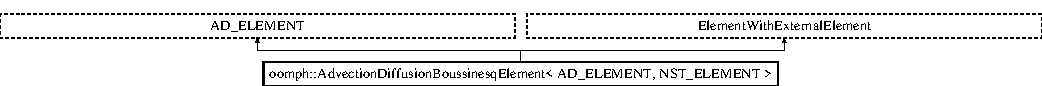
\includegraphics[height=1.161826cm]{classoomph_1_1AdvectionDiffusionBoussinesqElement}
\end{center}
\end{figure}
\subsection*{Public Member Functions}
\begin{DoxyCompactItemize}
\item 
\hyperlink{classoomph_1_1AdvectionDiffusionBoussinesqElement_a733c18518938e3b85e06de5a618cd49f}{Advection\+Diffusion\+Boussinesq\+Element} ()
\begin{DoxyCompactList}\small\item\em Constructor\+: call the underlying constructors. \end{DoxyCompactList}\item 
void \hyperlink{classoomph_1_1AdvectionDiffusionBoussinesqElement_a86ec5858acc0a562cee7bccedfecb252}{get\+\_\+wind\+\_\+adv\+\_\+diff} (const unsigned \&ipt, const Vector$<$ double $>$ \&s, const Vector$<$ double $>$ \&x, Vector$<$ double $>$ \&wind) const
\begin{DoxyCompactList}\small\item\em Overload the wind function in the advection-\/diffusion equations. This provides the coupling from the Navier--Stokes equations to the advection-\/diffusion equations because the wind is the fluid velocity, obtained from the source element in the other mesh. \end{DoxyCompactList}\item 
void \hyperlink{classoomph_1_1AdvectionDiffusionBoussinesqElement_afcb2b136650ecca8fd47eb4278616d29}{output} (std\+::ostream \&outfile, const unsigned \&nplot)
\begin{DoxyCompactList}\small\item\em Output function\+: Output x, y, theta at Nplot$^\wedge$\+D\+IM plot points. \end{DoxyCompactList}\item 
void \hyperlink{classoomph_1_1AdvectionDiffusionBoussinesqElement_acc615c265bef2c3f5c30c6be95c0f50d}{output} (std\+::ostream \&outfile)
\begin{DoxyCompactList}\small\item\em Overload the standard output function with the broken default. \end{DoxyCompactList}\item 
void \hyperlink{classoomph_1_1AdvectionDiffusionBoussinesqElement_adbd60fca6201bc2cd80ff39303323053}{output} (F\+I\+LE $\ast$file\+\_\+pt)
\begin{DoxyCompactList}\small\item\em C-\/style output function\+: Broken default. \end{DoxyCompactList}\item 
void \hyperlink{classoomph_1_1AdvectionDiffusionBoussinesqElement_adbe60877f205b36d76a87695afb28caa}{output} (F\+I\+LE $\ast$file\+\_\+pt, const unsigned \&n\+\_\+plot)
\begin{DoxyCompactList}\small\item\em C-\/style output function\+: Broken default. \end{DoxyCompactList}\item 
void \hyperlink{classoomph_1_1AdvectionDiffusionBoussinesqElement_a89ea74af5d011a3866999c3760621edf}{get\+\_\+dwind\+\_\+adv\+\_\+diff\+\_\+dexternal\+\_\+element\+\_\+data} (const unsigned \&ipt, const unsigned \&i, Vector$<$ double $>$ \&result, Vector$<$ unsigned $>$ \&global\+\_\+eqn\+\_\+number)
\begin{DoxyCompactList}\small\item\em Fill in the derivatives of the wind with respect to the external unknowns. \end{DoxyCompactList}\item 
void \hyperlink{classoomph_1_1AdvectionDiffusionBoussinesqElement_afc63db5ad4e397df7809447ee3ca56ac}{fill\+\_\+in\+\_\+contribution\+\_\+to\+\_\+jacobian} (Vector$<$ double $>$ \&residuals, Dense\+Matrix$<$ double $>$ \&jacobian)
\begin{DoxyCompactList}\small\item\em Compute the element\textquotesingle{}s residual vector and the Jacobian matrix. Jacobian is computed by finite-\/differencing. \end{DoxyCompactList}\item 
void \hyperlink{classoomph_1_1AdvectionDiffusionBoussinesqElement_a375fb98e225dbd5ac716ed3f68831069}{fill\+\_\+in\+\_\+contribution\+\_\+to\+\_\+jacobian\+\_\+and\+\_\+mass\+\_\+matrix} (Vector$<$ double $>$ \&residuals, Dense\+Matrix$<$ double $>$ \&jacobian, Dense\+Matrix$<$ double $>$ \&mass\+\_\+matrix)
\begin{DoxyCompactList}\small\item\em Add the element\textquotesingle{}s contribution to its residuals vector, jacobian matrix and mass matrix. \end{DoxyCompactList}\item 
void \hyperlink{classoomph_1_1AdvectionDiffusionBoussinesqElement_a9e859b487d8398ae696de72104c76271}{fill\+\_\+in\+\_\+off\+\_\+diagonal\+\_\+block\+\_\+analytic} (Vector$<$ double $>$ \&residuals, Dense\+Matrix$<$ double $>$ \&jacobian)
\begin{DoxyCompactList}\small\item\em Compute the contribution of the external degrees of freedom (velocities) on the Advection\+Diffusion equations. \end{DoxyCompactList}\end{DoxyCompactItemize}


\subsection{Detailed Description}
\subsubsection*{template$<$class A\+D\+\_\+\+E\+L\+E\+M\+E\+NT, class N\+S\+T\+\_\+\+E\+L\+E\+M\+E\+NT$>$\newline
class oomph\+::\+Advection\+Diffusion\+Boussinesq\+Element$<$ A\+D\+\_\+\+E\+L\+E\+M\+E\+N\+T, N\+S\+T\+\_\+\+E\+L\+E\+M\+E\+N\+T $>$}

Build \hyperlink{classoomph_1_1AdvectionDiffusionBoussinesqElement}{Advection\+Diffusion\+Boussinesq\+Element} that inherits from Element\+With\+External\+Element so that it can \char`\"{}communicate\char`\"{} with the Navier Stokes element 

Definition at line 1054 of file multi\+\_\+domain\+\_\+boussinesq\+\_\+elements.\+h.



\subsection{Constructor \& Destructor Documentation}
\mbox{\Hypertarget{classoomph_1_1AdvectionDiffusionBoussinesqElement_a733c18518938e3b85e06de5a618cd49f}\label{classoomph_1_1AdvectionDiffusionBoussinesqElement_a733c18518938e3b85e06de5a618cd49f}} 
\index{oomph\+::\+Advection\+Diffusion\+Boussinesq\+Element@{oomph\+::\+Advection\+Diffusion\+Boussinesq\+Element}!Advection\+Diffusion\+Boussinesq\+Element@{Advection\+Diffusion\+Boussinesq\+Element}}
\index{Advection\+Diffusion\+Boussinesq\+Element@{Advection\+Diffusion\+Boussinesq\+Element}!oomph\+::\+Advection\+Diffusion\+Boussinesq\+Element@{oomph\+::\+Advection\+Diffusion\+Boussinesq\+Element}}
\subsubsection{\texorpdfstring{Advection\+Diffusion\+Boussinesq\+Element()}{AdvectionDiffusionBoussinesqElement()}}
{\footnotesize\ttfamily template$<$class A\+D\+\_\+\+E\+L\+E\+M\+E\+NT , class N\+S\+T\+\_\+\+E\+L\+E\+M\+E\+NT $>$ \\
\hyperlink{classoomph_1_1AdvectionDiffusionBoussinesqElement}{oomph\+::\+Advection\+Diffusion\+Boussinesq\+Element}$<$ A\+D\+\_\+\+E\+L\+E\+M\+E\+NT, N\+S\+T\+\_\+\+E\+L\+E\+M\+E\+NT $>$\+::\hyperlink{classoomph_1_1AdvectionDiffusionBoussinesqElement}{Advection\+Diffusion\+Boussinesq\+Element} (\begin{DoxyParamCaption}{ }\end{DoxyParamCaption})\hspace{0.3cm}{\ttfamily [inline]}}



Constructor\+: call the underlying constructors. 



Definition at line 1061 of file multi\+\_\+domain\+\_\+boussinesq\+\_\+elements.\+h.



\subsection{Member Function Documentation}
\mbox{\Hypertarget{classoomph_1_1AdvectionDiffusionBoussinesqElement_afc63db5ad4e397df7809447ee3ca56ac}\label{classoomph_1_1AdvectionDiffusionBoussinesqElement_afc63db5ad4e397df7809447ee3ca56ac}} 
\index{oomph\+::\+Advection\+Diffusion\+Boussinesq\+Element@{oomph\+::\+Advection\+Diffusion\+Boussinesq\+Element}!fill\+\_\+in\+\_\+contribution\+\_\+to\+\_\+jacobian@{fill\+\_\+in\+\_\+contribution\+\_\+to\+\_\+jacobian}}
\index{fill\+\_\+in\+\_\+contribution\+\_\+to\+\_\+jacobian@{fill\+\_\+in\+\_\+contribution\+\_\+to\+\_\+jacobian}!oomph\+::\+Advection\+Diffusion\+Boussinesq\+Element@{oomph\+::\+Advection\+Diffusion\+Boussinesq\+Element}}
\subsubsection{\texorpdfstring{fill\+\_\+in\+\_\+contribution\+\_\+to\+\_\+jacobian()}{fill\_in\_contribution\_to\_jacobian()}}
{\footnotesize\ttfamily template$<$class A\+D\+\_\+\+E\+L\+E\+M\+E\+NT , class N\+S\+T\+\_\+\+E\+L\+E\+M\+E\+NT $>$ \\
void \hyperlink{classoomph_1_1AdvectionDiffusionBoussinesqElement}{oomph\+::\+Advection\+Diffusion\+Boussinesq\+Element}$<$ A\+D\+\_\+\+E\+L\+E\+M\+E\+NT, N\+S\+T\+\_\+\+E\+L\+E\+M\+E\+NT $>$\+::fill\+\_\+in\+\_\+contribution\+\_\+to\+\_\+jacobian (\begin{DoxyParamCaption}\item[{Vector$<$ double $>$ \&}]{residuals,  }\item[{Dense\+Matrix$<$ double $>$ \&}]{jacobian }\end{DoxyParamCaption})\hspace{0.3cm}{\ttfamily [inline]}}



Compute the element\textquotesingle{}s residual vector and the Jacobian matrix. Jacobian is computed by finite-\/differencing. 



Definition at line 1142 of file multi\+\_\+domain\+\_\+boussinesq\+\_\+elements.\+h.

\mbox{\Hypertarget{classoomph_1_1AdvectionDiffusionBoussinesqElement_a375fb98e225dbd5ac716ed3f68831069}\label{classoomph_1_1AdvectionDiffusionBoussinesqElement_a375fb98e225dbd5ac716ed3f68831069}} 
\index{oomph\+::\+Advection\+Diffusion\+Boussinesq\+Element@{oomph\+::\+Advection\+Diffusion\+Boussinesq\+Element}!fill\+\_\+in\+\_\+contribution\+\_\+to\+\_\+jacobian\+\_\+and\+\_\+mass\+\_\+matrix@{fill\+\_\+in\+\_\+contribution\+\_\+to\+\_\+jacobian\+\_\+and\+\_\+mass\+\_\+matrix}}
\index{fill\+\_\+in\+\_\+contribution\+\_\+to\+\_\+jacobian\+\_\+and\+\_\+mass\+\_\+matrix@{fill\+\_\+in\+\_\+contribution\+\_\+to\+\_\+jacobian\+\_\+and\+\_\+mass\+\_\+matrix}!oomph\+::\+Advection\+Diffusion\+Boussinesq\+Element@{oomph\+::\+Advection\+Diffusion\+Boussinesq\+Element}}
\subsubsection{\texorpdfstring{fill\+\_\+in\+\_\+contribution\+\_\+to\+\_\+jacobian\+\_\+and\+\_\+mass\+\_\+matrix()}{fill\_in\_contribution\_to\_jacobian\_and\_mass\_matrix()}}
{\footnotesize\ttfamily template$<$class A\+D\+\_\+\+E\+L\+E\+M\+E\+NT , class N\+S\+T\+\_\+\+E\+L\+E\+M\+E\+NT $>$ \\
void \hyperlink{classoomph_1_1AdvectionDiffusionBoussinesqElement}{oomph\+::\+Advection\+Diffusion\+Boussinesq\+Element}$<$ A\+D\+\_\+\+E\+L\+E\+M\+E\+NT, N\+S\+T\+\_\+\+E\+L\+E\+M\+E\+NT $>$\+::fill\+\_\+in\+\_\+contribution\+\_\+to\+\_\+jacobian\+\_\+and\+\_\+mass\+\_\+matrix (\begin{DoxyParamCaption}\item[{Vector$<$ double $>$ \&}]{residuals,  }\item[{Dense\+Matrix$<$ double $>$ \&}]{jacobian,  }\item[{Dense\+Matrix$<$ double $>$ \&}]{mass\+\_\+matrix }\end{DoxyParamCaption})\hspace{0.3cm}{\ttfamily [inline]}}



Add the element\textquotesingle{}s contribution to its residuals vector, jacobian matrix and mass matrix. 



Definition at line 1164 of file multi\+\_\+domain\+\_\+boussinesq\+\_\+elements.\+h.

\mbox{\Hypertarget{classoomph_1_1AdvectionDiffusionBoussinesqElement_a9e859b487d8398ae696de72104c76271}\label{classoomph_1_1AdvectionDiffusionBoussinesqElement_a9e859b487d8398ae696de72104c76271}} 
\index{oomph\+::\+Advection\+Diffusion\+Boussinesq\+Element@{oomph\+::\+Advection\+Diffusion\+Boussinesq\+Element}!fill\+\_\+in\+\_\+off\+\_\+diagonal\+\_\+block\+\_\+analytic@{fill\+\_\+in\+\_\+off\+\_\+diagonal\+\_\+block\+\_\+analytic}}
\index{fill\+\_\+in\+\_\+off\+\_\+diagonal\+\_\+block\+\_\+analytic@{fill\+\_\+in\+\_\+off\+\_\+diagonal\+\_\+block\+\_\+analytic}!oomph\+::\+Advection\+Diffusion\+Boussinesq\+Element@{oomph\+::\+Advection\+Diffusion\+Boussinesq\+Element}}
\subsubsection{\texorpdfstring{fill\+\_\+in\+\_\+off\+\_\+diagonal\+\_\+block\+\_\+analytic()}{fill\_in\_off\_diagonal\_block\_analytic()}}
{\footnotesize\ttfamily template$<$class A\+D\+\_\+\+E\+L\+E\+M\+E\+NT , class N\+S\+T\+\_\+\+E\+L\+E\+M\+E\+NT $>$ \\
void \hyperlink{classoomph_1_1AdvectionDiffusionBoussinesqElement}{oomph\+::\+Advection\+Diffusion\+Boussinesq\+Element}$<$ A\+D\+\_\+\+E\+L\+E\+M\+E\+NT, N\+S\+T\+\_\+\+E\+L\+E\+M\+E\+NT $>$\+::fill\+\_\+in\+\_\+off\+\_\+diagonal\+\_\+block\+\_\+analytic (\begin{DoxyParamCaption}\item[{Vector$<$ double $>$ \&}]{residuals,  }\item[{Dense\+Matrix$<$ double $>$ \&}]{jacobian }\end{DoxyParamCaption})\hspace{0.3cm}{\ttfamily [inline]}}



Compute the contribution of the external degrees of freedom (velocities) on the Advection\+Diffusion equations. 



Definition at line 1178 of file multi\+\_\+domain\+\_\+boussinesq\+\_\+elements.\+h.



References oomph\+::\+Advection\+Diffusion\+Boussinesq\+Element$<$ A\+D\+\_\+\+E\+L\+E\+M\+E\+N\+T, N\+S\+T\+\_\+\+E\+L\+E\+M\+E\+N\+T $>$\+::get\+\_\+wind\+\_\+adv\+\_\+diff().

\mbox{\Hypertarget{classoomph_1_1AdvectionDiffusionBoussinesqElement_a89ea74af5d011a3866999c3760621edf}\label{classoomph_1_1AdvectionDiffusionBoussinesqElement_a89ea74af5d011a3866999c3760621edf}} 
\index{oomph\+::\+Advection\+Diffusion\+Boussinesq\+Element@{oomph\+::\+Advection\+Diffusion\+Boussinesq\+Element}!get\+\_\+dwind\+\_\+adv\+\_\+diff\+\_\+dexternal\+\_\+element\+\_\+data@{get\+\_\+dwind\+\_\+adv\+\_\+diff\+\_\+dexternal\+\_\+element\+\_\+data}}
\index{get\+\_\+dwind\+\_\+adv\+\_\+diff\+\_\+dexternal\+\_\+element\+\_\+data@{get\+\_\+dwind\+\_\+adv\+\_\+diff\+\_\+dexternal\+\_\+element\+\_\+data}!oomph\+::\+Advection\+Diffusion\+Boussinesq\+Element@{oomph\+::\+Advection\+Diffusion\+Boussinesq\+Element}}
\subsubsection{\texorpdfstring{get\+\_\+dwind\+\_\+adv\+\_\+diff\+\_\+dexternal\+\_\+element\+\_\+data()}{get\_dwind\_adv\_diff\_dexternal\_element\_data()}}
{\footnotesize\ttfamily template$<$class A\+D\+\_\+\+E\+L\+E\+M\+E\+NT , class N\+S\+T\+\_\+\+E\+L\+E\+M\+E\+NT $>$ \\
void \hyperlink{classoomph_1_1AdvectionDiffusionBoussinesqElement}{oomph\+::\+Advection\+Diffusion\+Boussinesq\+Element}$<$ A\+D\+\_\+\+E\+L\+E\+M\+E\+NT, N\+S\+T\+\_\+\+E\+L\+E\+M\+E\+NT $>$\+::get\+\_\+dwind\+\_\+adv\+\_\+diff\+\_\+dexternal\+\_\+element\+\_\+data (\begin{DoxyParamCaption}\item[{const unsigned \&}]{ipt,  }\item[{const unsigned \&}]{i,  }\item[{Vector$<$ double $>$ \&}]{result,  }\item[{Vector$<$ unsigned $>$ \&}]{global\+\_\+eqn\+\_\+number }\end{DoxyParamCaption})}



Fill in the derivatives of the wind with respect to the external unknowns. 

Fill in the derivatives of the wind with respect to the external unknowns in the advection-\/diffusion equations 

Definition at line 1317 of file multi\+\_\+domain\+\_\+boussinesq\+\_\+elements.\+h.



References oomph\+::\+Navier\+Stokes\+Boussinesq\+Element$<$ N\+S\+T\+\_\+\+E\+L\+E\+M\+E\+N\+T, A\+D\+\_\+\+E\+L\+E\+M\+E\+N\+T $>$\+::get\+\_\+dbody\+\_\+force\+\_\+nst\+\_\+dexternal\+\_\+element\+\_\+data().



Referenced by oomph\+::\+Advection\+Diffusion\+Boussinesq\+Element$<$ A\+D\+\_\+\+E\+L\+E\+M\+E\+N\+T, N\+S\+T\+\_\+\+E\+L\+E\+M\+E\+N\+T $>$\+::get\+\_\+wind\+\_\+adv\+\_\+diff().

\mbox{\Hypertarget{classoomph_1_1AdvectionDiffusionBoussinesqElement_a86ec5858acc0a562cee7bccedfecb252}\label{classoomph_1_1AdvectionDiffusionBoussinesqElement_a86ec5858acc0a562cee7bccedfecb252}} 
\index{oomph\+::\+Advection\+Diffusion\+Boussinesq\+Element@{oomph\+::\+Advection\+Diffusion\+Boussinesq\+Element}!get\+\_\+wind\+\_\+adv\+\_\+diff@{get\+\_\+wind\+\_\+adv\+\_\+diff}}
\index{get\+\_\+wind\+\_\+adv\+\_\+diff@{get\+\_\+wind\+\_\+adv\+\_\+diff}!oomph\+::\+Advection\+Diffusion\+Boussinesq\+Element@{oomph\+::\+Advection\+Diffusion\+Boussinesq\+Element}}
\subsubsection{\texorpdfstring{get\+\_\+wind\+\_\+adv\+\_\+diff()}{get\_wind\_adv\_diff()}}
{\footnotesize\ttfamily template$<$class A\+D\+\_\+\+E\+L\+E\+M\+E\+NT , class N\+S\+T\+\_\+\+E\+L\+E\+M\+E\+NT $>$ \\
void \hyperlink{classoomph_1_1AdvectionDiffusionBoussinesqElement}{oomph\+::\+Advection\+Diffusion\+Boussinesq\+Element}$<$ A\+D\+\_\+\+E\+L\+E\+M\+E\+NT, N\+S\+T\+\_\+\+E\+L\+E\+M\+E\+NT $>$\+::get\+\_\+wind\+\_\+adv\+\_\+diff (\begin{DoxyParamCaption}\item[{const unsigned \&}]{ipt,  }\item[{const Vector$<$ double $>$ \&}]{s,  }\item[{const Vector$<$ double $>$ \&}]{x,  }\item[{Vector$<$ double $>$ \&}]{wind }\end{DoxyParamCaption}) const}



Overload the wind function in the advection-\/diffusion equations. This provides the coupling from the Navier--Stokes equations to the advection-\/diffusion equations because the wind is the fluid velocity, obtained from the source element in the other mesh. 

Overload the wind function in the advection-\/diffusion equations. This provides the coupling from the Navier--Stokes equations to the advection-\/diffusion equations because the wind is the fluid velocity, obtained from the source elements in the other mesh. 

Definition at line 1296 of file multi\+\_\+domain\+\_\+boussinesq\+\_\+elements.\+h.



References oomph\+::\+Advection\+Diffusion\+Boussinesq\+Element$<$ A\+D\+\_\+\+E\+L\+E\+M\+E\+N\+T, N\+S\+T\+\_\+\+E\+L\+E\+M\+E\+N\+T $>$\+::get\+\_\+dwind\+\_\+adv\+\_\+diff\+\_\+dexternal\+\_\+element\+\_\+data().



Referenced by oomph\+::\+Advection\+Diffusion\+Boussinesq\+Element$<$ A\+D\+\_\+\+E\+L\+E\+M\+E\+N\+T, N\+S\+T\+\_\+\+E\+L\+E\+M\+E\+N\+T $>$\+::fill\+\_\+in\+\_\+off\+\_\+diagonal\+\_\+block\+\_\+analytic().

\mbox{\Hypertarget{classoomph_1_1AdvectionDiffusionBoussinesqElement_afcb2b136650ecca8fd47eb4278616d29}\label{classoomph_1_1AdvectionDiffusionBoussinesqElement_afcb2b136650ecca8fd47eb4278616d29}} 
\index{oomph\+::\+Advection\+Diffusion\+Boussinesq\+Element@{oomph\+::\+Advection\+Diffusion\+Boussinesq\+Element}!output@{output}}
\index{output@{output}!oomph\+::\+Advection\+Diffusion\+Boussinesq\+Element@{oomph\+::\+Advection\+Diffusion\+Boussinesq\+Element}}
\subsubsection{\texorpdfstring{output()}{output()}\hspace{0.1cm}{\footnotesize\ttfamily [1/4]}}
{\footnotesize\ttfamily template$<$class A\+D\+\_\+\+E\+L\+E\+M\+E\+NT , class N\+S\+T\+\_\+\+E\+L\+E\+M\+E\+NT $>$ \\
void \hyperlink{classoomph_1_1AdvectionDiffusionBoussinesqElement}{oomph\+::\+Advection\+Diffusion\+Boussinesq\+Element}$<$ A\+D\+\_\+\+E\+L\+E\+M\+E\+NT, N\+S\+T\+\_\+\+E\+L\+E\+M\+E\+NT $>$\+::output (\begin{DoxyParamCaption}\item[{std\+::ostream \&}]{outfile,  }\item[{const unsigned \&}]{nplot }\end{DoxyParamCaption})\hspace{0.3cm}{\ttfamily [inline]}}



Output function\+: Output x, y, theta at Nplot$^\wedge$\+D\+IM plot points. 



Definition at line 1087 of file multi\+\_\+domain\+\_\+boussinesq\+\_\+elements.\+h.

\mbox{\Hypertarget{classoomph_1_1AdvectionDiffusionBoussinesqElement_acc615c265bef2c3f5c30c6be95c0f50d}\label{classoomph_1_1AdvectionDiffusionBoussinesqElement_acc615c265bef2c3f5c30c6be95c0f50d}} 
\index{oomph\+::\+Advection\+Diffusion\+Boussinesq\+Element@{oomph\+::\+Advection\+Diffusion\+Boussinesq\+Element}!output@{output}}
\index{output@{output}!oomph\+::\+Advection\+Diffusion\+Boussinesq\+Element@{oomph\+::\+Advection\+Diffusion\+Boussinesq\+Element}}
\subsubsection{\texorpdfstring{output()}{output()}\hspace{0.1cm}{\footnotesize\ttfamily [2/4]}}
{\footnotesize\ttfamily template$<$class A\+D\+\_\+\+E\+L\+E\+M\+E\+NT , class N\+S\+T\+\_\+\+E\+L\+E\+M\+E\+NT $>$ \\
void \hyperlink{classoomph_1_1AdvectionDiffusionBoussinesqElement}{oomph\+::\+Advection\+Diffusion\+Boussinesq\+Element}$<$ A\+D\+\_\+\+E\+L\+E\+M\+E\+NT, N\+S\+T\+\_\+\+E\+L\+E\+M\+E\+NT $>$\+::output (\begin{DoxyParamCaption}\item[{std\+::ostream \&}]{outfile }\end{DoxyParamCaption})\hspace{0.3cm}{\ttfamily [inline]}}



Overload the standard output function with the broken default. 



Definition at line 1121 of file multi\+\_\+domain\+\_\+boussinesq\+\_\+elements.\+h.

\mbox{\Hypertarget{classoomph_1_1AdvectionDiffusionBoussinesqElement_adbd60fca6201bc2cd80ff39303323053}\label{classoomph_1_1AdvectionDiffusionBoussinesqElement_adbd60fca6201bc2cd80ff39303323053}} 
\index{oomph\+::\+Advection\+Diffusion\+Boussinesq\+Element@{oomph\+::\+Advection\+Diffusion\+Boussinesq\+Element}!output@{output}}
\index{output@{output}!oomph\+::\+Advection\+Diffusion\+Boussinesq\+Element@{oomph\+::\+Advection\+Diffusion\+Boussinesq\+Element}}
\subsubsection{\texorpdfstring{output()}{output()}\hspace{0.1cm}{\footnotesize\ttfamily [3/4]}}
{\footnotesize\ttfamily template$<$class A\+D\+\_\+\+E\+L\+E\+M\+E\+NT , class N\+S\+T\+\_\+\+E\+L\+E\+M\+E\+NT $>$ \\
void \hyperlink{classoomph_1_1AdvectionDiffusionBoussinesqElement}{oomph\+::\+Advection\+Diffusion\+Boussinesq\+Element}$<$ A\+D\+\_\+\+E\+L\+E\+M\+E\+NT, N\+S\+T\+\_\+\+E\+L\+E\+M\+E\+NT $>$\+::output (\begin{DoxyParamCaption}\item[{F\+I\+LE $\ast$}]{file\+\_\+pt }\end{DoxyParamCaption})\hspace{0.3cm}{\ttfamily [inline]}}



C-\/style output function\+: Broken default. 



Definition at line 1124 of file multi\+\_\+domain\+\_\+boussinesq\+\_\+elements.\+h.

\mbox{\Hypertarget{classoomph_1_1AdvectionDiffusionBoussinesqElement_adbe60877f205b36d76a87695afb28caa}\label{classoomph_1_1AdvectionDiffusionBoussinesqElement_adbe60877f205b36d76a87695afb28caa}} 
\index{oomph\+::\+Advection\+Diffusion\+Boussinesq\+Element@{oomph\+::\+Advection\+Diffusion\+Boussinesq\+Element}!output@{output}}
\index{output@{output}!oomph\+::\+Advection\+Diffusion\+Boussinesq\+Element@{oomph\+::\+Advection\+Diffusion\+Boussinesq\+Element}}
\subsubsection{\texorpdfstring{output()}{output()}\hspace{0.1cm}{\footnotesize\ttfamily [4/4]}}
{\footnotesize\ttfamily template$<$class A\+D\+\_\+\+E\+L\+E\+M\+E\+NT , class N\+S\+T\+\_\+\+E\+L\+E\+M\+E\+NT $>$ \\
void \hyperlink{classoomph_1_1AdvectionDiffusionBoussinesqElement}{oomph\+::\+Advection\+Diffusion\+Boussinesq\+Element}$<$ A\+D\+\_\+\+E\+L\+E\+M\+E\+NT, N\+S\+T\+\_\+\+E\+L\+E\+M\+E\+NT $>$\+::output (\begin{DoxyParamCaption}\item[{F\+I\+LE $\ast$}]{file\+\_\+pt,  }\item[{const unsigned \&}]{n\+\_\+plot }\end{DoxyParamCaption})\hspace{0.3cm}{\ttfamily [inline]}}



C-\/style output function\+: Broken default. 



Definition at line 1128 of file multi\+\_\+domain\+\_\+boussinesq\+\_\+elements.\+h.



The documentation for this class was generated from the following file\+:\begin{DoxyCompactItemize}
\item 
\hyperlink{multi__domain__boussinesq__elements_8h}{multi\+\_\+domain\+\_\+boussinesq\+\_\+elements.\+h}\end{DoxyCompactItemize}

\hypertarget{classoomph_1_1BuoyantQCrouzeixRaviartElement}{}\section{oomph\+:\+:Buoyant\+Q\+Crouzeix\+Raviart\+Element$<$ D\+IM $>$ Class Template Reference}
\label{classoomph_1_1BuoyantQCrouzeixRaviartElement}\index{oomph\+::\+Buoyant\+Q\+Crouzeix\+Raviart\+Element$<$ D\+I\+M $>$@{oomph\+::\+Buoyant\+Q\+Crouzeix\+Raviart\+Element$<$ D\+I\+M $>$}}


{\ttfamily \#include $<$boussinesq\+\_\+elements.\+h$>$}

Inheritance diagram for oomph\+:\+:Buoyant\+Q\+Crouzeix\+Raviart\+Element$<$ D\+IM $>$\+:\begin{figure}[H]
\begin{center}
\leavevmode
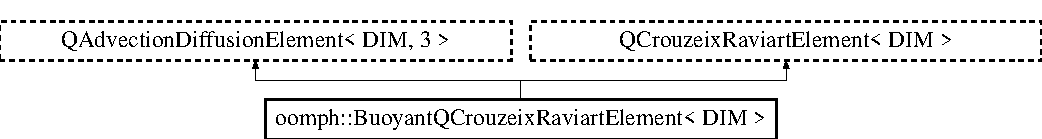
\includegraphics[height=1.866667cm]{classoomph_1_1BuoyantQCrouzeixRaviartElement}
\end{center}
\end{figure}
\subsection*{Public Member Functions}
\begin{DoxyCompactItemize}
\item 
\hyperlink{classoomph_1_1BuoyantQCrouzeixRaviartElement_a9651742d190071d973ed5c154341d82b}{Buoyant\+Q\+Crouzeix\+Raviart\+Element} ()
\begin{DoxyCompactList}\small\item\em Constructor\+: call the underlying constructors and initialise the pointer to the Rayleigh number to point to the default value of 0.\+0. \end{DoxyCompactList}\item 
void \hyperlink{classoomph_1_1BuoyantQCrouzeixRaviartElement_a9468f7a594a5b9a9a07d3bf27dbcff45}{unfix\+\_\+pressure} (const unsigned \&p\+\_\+dof)
\begin{DoxyCompactList}\small\item\em Unpin p\+\_\+dof-\/th pressure dof. \end{DoxyCompactList}\item 
unsigned \hyperlink{classoomph_1_1BuoyantQCrouzeixRaviartElement_a64b84c9cf74a06680136d465ff9e037b}{required\+\_\+nvalue} (const unsigned \&n) const
\begin{DoxyCompactList}\small\item\em The required number of values stored at the nodes is the sum of the required values of the two single-\/physics elements. Note that this step is generic for any multi-\/physics element of this type. \end{DoxyCompactList}\item 
const double \& \hyperlink{classoomph_1_1BuoyantQCrouzeixRaviartElement_a5876310641d9f5028de6d4263013e247}{ra} () const
\begin{DoxyCompactList}\small\item\em Access function for the Rayleigh number (const version) \end{DoxyCompactList}\item 
double $\ast$\& \hyperlink{classoomph_1_1BuoyantQCrouzeixRaviartElement_afa4d4ff16fa307b16feab1de7aaa90b6}{ra\+\_\+pt} ()
\begin{DoxyCompactList}\small\item\em Access function for the pointer to the Rayleigh number. \end{DoxyCompactList}\item 
void \hyperlink{classoomph_1_1BuoyantQCrouzeixRaviartElement_a534fc134280b7447eecc4cad46b2e4c5}{disable\+\_\+\+A\+LE} ()
\begin{DoxyCompactList}\small\item\em Final override for disable A\+LE. \end{DoxyCompactList}\item 
void \hyperlink{classoomph_1_1BuoyantQCrouzeixRaviartElement_af551bb70aa118a8db4498f41272fe776}{enable\+\_\+\+A\+LE} ()
\begin{DoxyCompactList}\small\item\em Final override for enable A\+LE. \end{DoxyCompactList}\item 
unsigned \hyperlink{classoomph_1_1BuoyantQCrouzeixRaviartElement_a5103e49416e1a0e36a2e8e117fb78623}{nscalar\+\_\+paraview} () const
\begin{DoxyCompactList}\small\item\em Number of scalars/fields output by this element. Broken virtual. Needs to be implemented for each new specific element type. Temporary dummy. \end{DoxyCompactList}\item 
void \hyperlink{classoomph_1_1BuoyantQCrouzeixRaviartElement_a33130eacdbdee41536fce76166c4a769}{scalar\+\_\+value\+\_\+paraview} (std\+::ofstream \&file\+\_\+out, const unsigned \&i, const unsigned \&nplot) const
\begin{DoxyCompactList}\small\item\em Write values of the i-\/th scalar field at the plot points. Broken virtual. Needs to be implemented for each new specific element type. Temporary dummy. \end{DoxyCompactList}\item 
std\+::string \hyperlink{classoomph_1_1BuoyantQCrouzeixRaviartElement_a26f8112d2ba9c77087e534145a2477c9}{scalar\+\_\+name\+\_\+paraview} (const unsigned \&i) const
\begin{DoxyCompactList}\small\item\em Name of the i-\/th scalar field. Default implementation returns V1 for the first one, V2 for the second etc. Can (should!) be overloaded with more meaningful names. \end{DoxyCompactList}\item 
void \hyperlink{classoomph_1_1BuoyantQCrouzeixRaviartElement_a3817706dbf3c755b4029917dac80bad7}{output} (std\+::ostream \&outfile)
\begin{DoxyCompactList}\small\item\em Overload the standard output function with the broken default. \end{DoxyCompactList}\item 
void \hyperlink{classoomph_1_1BuoyantQCrouzeixRaviartElement_a855783400ac22a61e151d1611ad8e47e}{output} (std\+::ostream \&outfile, const unsigned \&nplot)
\begin{DoxyCompactList}\small\item\em Output function\+: Output x, y, u, v, p, theta at Nplot$^\wedge$\+D\+IM plot points. \end{DoxyCompactList}\item 
void \hyperlink{classoomph_1_1BuoyantQCrouzeixRaviartElement_a9ba77409f12b80862262f6695829055b}{output} (F\+I\+LE $\ast$file\+\_\+pt)
\begin{DoxyCompactList}\small\item\em C-\/style output function\+: Broken default. \end{DoxyCompactList}\item 
void \hyperlink{classoomph_1_1BuoyantQCrouzeixRaviartElement_a48039bbb2f32897b70fb0858ff739516}{output} (F\+I\+LE $\ast$file\+\_\+pt, const unsigned \&n\+\_\+plot)
\begin{DoxyCompactList}\small\item\em C-\/style output function\+: Broken default. \end{DoxyCompactList}\item 
void \hyperlink{classoomph_1_1BuoyantQCrouzeixRaviartElement_ad36c2a18f2de8b00f76baccc15b768c2}{output\+\_\+fct} (std\+::ostream \&outfile, const unsigned \&Nplot, Finite\+Element\+::\+Steady\+Exact\+Solution\+Fct\+Pt exact\+\_\+soln\+\_\+pt)
\begin{DoxyCompactList}\small\item\em Output function for an exact solution\+: Broken default. \end{DoxyCompactList}\item 
void \hyperlink{classoomph_1_1BuoyantQCrouzeixRaviartElement_ae1c6dc6850532af9ec618415ba31e053}{output\+\_\+fct} (std\+::ostream \&outfile, const unsigned \&Nplot, const double \&time, Finite\+Element\+::\+Unsteady\+Exact\+Solution\+Fct\+Pt exact\+\_\+soln\+\_\+pt)
\begin{DoxyCompactList}\small\item\em Output function for a time-\/dependent exact solution\+: Broken default. \end{DoxyCompactList}\item 
unsigned \hyperlink{classoomph_1_1BuoyantQCrouzeixRaviartElement_acf5fa44f694c5374c61a964020437bf4}{u\+\_\+index\+\_\+adv\+\_\+diff} () const
\begin{DoxyCompactList}\small\item\em Overload the index at which the temperature variable is stored. We choose to store it after the fluid velocities. \end{DoxyCompactList}\item 
void \hyperlink{classoomph_1_1BuoyantQCrouzeixRaviartElement_a53d343548b707c62e9f11a04d2dda986}{compute\+\_\+error} (std\+::ostream \&outfile, Finite\+Element\+::\+Unsteady\+Exact\+Solution\+Fct\+Pt exact\+\_\+soln\+\_\+pt, const double \&time, double \&error, double \&norm)
\begin{DoxyCompactList}\small\item\em Validate against exact solution at given time Solution is provided via function pointer. Plot at a given number of plot points and compute L2 error and L2 norm of velocity solution over element Call the broken default. \end{DoxyCompactList}\item 
void \hyperlink{classoomph_1_1BuoyantQCrouzeixRaviartElement_a2aa63b1b2ec1130835ee87cbf52cc086}{compute\+\_\+error} (std\+::ostream \&outfile, Finite\+Element\+::\+Steady\+Exact\+Solution\+Fct\+Pt exact\+\_\+soln\+\_\+pt, double \&error, double \&norm)
\begin{DoxyCompactList}\small\item\em Validate against exact solution. Solution is provided via function pointer. Plot at a given number of plot points and compute L2 error and L2 norm of velocity solution over element Call the broken default. \end{DoxyCompactList}\item 
void \hyperlink{classoomph_1_1BuoyantQCrouzeixRaviartElement_ade5820ae7c44a9371dcc348ca5a3ab1c}{get\+\_\+wind\+\_\+adv\+\_\+diff} (const unsigned \&ipt, const Vector$<$ double $>$ \&s, const Vector$<$ double $>$ \&x, Vector$<$ double $>$ \&wind) const
\begin{DoxyCompactList}\small\item\em Overload the wind function in the advection-\/diffusion equations. This provides the coupling from the Navier--Stokes equations to the advection-\/diffusion equations because the wind is the fluid velocity. \end{DoxyCompactList}\item 
void \hyperlink{classoomph_1_1BuoyantQCrouzeixRaviartElement_aeeef7868070fd692b33e5afa811af1da}{get\+\_\+body\+\_\+force\+\_\+nst} (const double \&time, const unsigned \&ipt, const Vector$<$ double $>$ \&s, const Vector$<$ double $>$ \&x, Vector$<$ double $>$ \&result)
\begin{DoxyCompactList}\small\item\em Overload the body force in the Navier-\/\+Stokes equations This provides the coupling from the advection-\/diffusion equations to the Navier--Stokes equations, the body force is the temperature multiplied by the Rayleigh number acting in the direction opposite to gravity. \end{DoxyCompactList}\item 
void \hyperlink{classoomph_1_1BuoyantQCrouzeixRaviartElement_ab87ed100a54d40884a70a67fcc305ecf}{fill\+\_\+in\+\_\+contribution\+\_\+to\+\_\+residuals} (Vector$<$ double $>$ \&residuals)
\begin{DoxyCompactList}\small\item\em Calculate the element\textquotesingle{}s contribution to the residual vector. Recall that fill\+\_\+in\+\_\+$\ast$ functions M\+U\+ST N\+OT initialise the entries in the vector to zero. This allows us to call the fill\+\_\+in\+\_\+$\ast$ functions of the constituent single-\/physics elements sequentially, without wiping out any previously computed entries. \end{DoxyCompactList}\item 
void \hyperlink{classoomph_1_1BuoyantQCrouzeixRaviartElement_a7bd9313dd697c1219cee4a65692388b5}{fill\+\_\+in\+\_\+contribution\+\_\+to\+\_\+jacobian} (Vector$<$ double $>$ \&residuals, Dense\+Matrix$<$ double $>$ \&jacobian)
\begin{DoxyCompactList}\small\item\em Compute the element\textquotesingle{}s residual vector and the Jacobian matrix. Jacobian is computed by finite-\/differencing. \end{DoxyCompactList}\item 
void \hyperlink{classoomph_1_1BuoyantQCrouzeixRaviartElement_a7d22156d87949e4c64d597d60fe00225}{fill\+\_\+in\+\_\+contribution\+\_\+to\+\_\+jacobian\+\_\+and\+\_\+mass\+\_\+matrix} (Vector$<$ double $>$ \&residuals, Dense\+Matrix$<$ double $>$ \&jacobian, Dense\+Matrix$<$ double $>$ \&mass\+\_\+matrix)
\item 
void \hyperlink{classoomph_1_1BuoyantQCrouzeixRaviartElement_a5c64aaf8e6cefc31d89c62c28fc6f19b}{fill\+\_\+in\+\_\+off\+\_\+diagonal\+\_\+jacobian\+\_\+blocks\+\_\+by\+\_\+fd} (Vector$<$ double $>$ \&residuals, Dense\+Matrix$<$ double $>$ \&jacobian)
\begin{DoxyCompactList}\small\item\em Helper function to get the off-\/diagonal blocks of the Jacobian matrix by finite differences. \end{DoxyCompactList}\item 
void \hyperlink{classoomph_1_1BuoyantQCrouzeixRaviartElement_a7bd9313dd697c1219cee4a65692388b5}{fill\+\_\+in\+\_\+contribution\+\_\+to\+\_\+jacobian} (Vector$<$ double $>$ \&residuals, Dense\+Matrix$<$ double $>$ \&jacobian)
\begin{DoxyCompactList}\small\item\em Compute the element\textquotesingle{}s residual Vector and the Jacobian matrix. Use finite-\/differencing only for the off-\/diagonal blocks. \end{DoxyCompactList}\item 
void \hyperlink{classoomph_1_1BuoyantQCrouzeixRaviartElement_a7d22156d87949e4c64d597d60fe00225}{fill\+\_\+in\+\_\+contribution\+\_\+to\+\_\+jacobian\+\_\+and\+\_\+mass\+\_\+matrix} (Vector$<$ double $>$ \&residuals, Dense\+Matrix$<$ double $>$ \&jacobian, Dense\+Matrix$<$ double $>$ \&mass\+\_\+matrix)
\item 
void \hyperlink{classoomph_1_1BuoyantQCrouzeixRaviartElement_aa344d9c1a36501baefc4afd56f227b94}{fill\+\_\+in\+\_\+off\+\_\+diagonal\+\_\+jacobian\+\_\+blocks\+\_\+analytic} (Vector$<$ double $>$ \&residuals, Dense\+Matrix$<$ double $>$ \&jacobian)
\begin{DoxyCompactList}\small\item\em Helper function to get the off-\/diagonal blocks of the Jacobian matrix analytically. \end{DoxyCompactList}\item 
void \hyperlink{classoomph_1_1BuoyantQCrouzeixRaviartElement_a7bd9313dd697c1219cee4a65692388b5}{fill\+\_\+in\+\_\+contribution\+\_\+to\+\_\+jacobian} (Vector$<$ double $>$ \&residuals, Dense\+Matrix$<$ double $>$ \&jacobian)
\begin{DoxyCompactList}\small\item\em Compute the element\textquotesingle{}s residual Vector and the Jacobian matrix. Use analytic expressions for the off-\/diagonal blocks. \end{DoxyCompactList}\item 
void \hyperlink{classoomph_1_1BuoyantQCrouzeixRaviartElement_a7d22156d87949e4c64d597d60fe00225}{fill\+\_\+in\+\_\+contribution\+\_\+to\+\_\+jacobian\+\_\+and\+\_\+mass\+\_\+matrix} (Vector$<$ double $>$ \&residuals, Dense\+Matrix$<$ double $>$ \&jacobian, Dense\+Matrix$<$ double $>$ \&mass\+\_\+matrix)
\end{DoxyCompactItemize}
\subsection*{Private Member Functions}
\begin{DoxyCompactItemize}
\item 
{\footnotesize template$<$$>$ }\\double \hyperlink{classoomph_1_1BuoyantQCrouzeixRaviartElement_a37e9dc4e6e5a8120a2f27587b5853086}{Default\+\_\+\+Physical\+\_\+\+Constant\+\_\+\+Value}
\begin{DoxyCompactList}\small\item\em Set the default physical value to be zero. \end{DoxyCompactList}\item 
{\footnotesize template$<$$>$ }\\double \hyperlink{classoomph_1_1BuoyantQCrouzeixRaviartElement_a74cccd0d2c7e943221f338fded0c18db}{Default\+\_\+\+Physical\+\_\+\+Constant\+\_\+\+Value}
\end{DoxyCompactItemize}
\subsection*{Private Attributes}
\begin{DoxyCompactItemize}
\item 
double $\ast$ \hyperlink{classoomph_1_1BuoyantQCrouzeixRaviartElement_a054ffb965ec8cce9b6b2da2336a1e7d8}{Ra\+\_\+pt}
\begin{DoxyCompactList}\small\item\em Pointer to a private data member, the Rayleigh number. \end{DoxyCompactList}\end{DoxyCompactItemize}
\subsection*{Static Private Attributes}
\begin{DoxyCompactItemize}
\item 
static double \hyperlink{classoomph_1_1BuoyantQCrouzeixRaviartElement_a3214e603f9b4108348c6a9abcede67ac}{Default\+\_\+\+Physical\+\_\+\+Constant\+\_\+\+Value}
\begin{DoxyCompactList}\small\item\em The static default value of the Rayleigh number. \end{DoxyCompactList}\end{DoxyCompactItemize}


\subsection{Detailed Description}
\subsubsection*{template$<$unsigned D\+IM$>$\newline
class oomph\+::\+Buoyant\+Q\+Crouzeix\+Raviart\+Element$<$ D\+I\+M $>$}

A class that solves the Boussinesq approximation of the Navier--Stokes and energy equations by coupling two pre-\/existing classes. The Q\+Advection\+Diffusion\+Element with bi-\/quadratic interpolation for the scalar variable (temperature) and Q\+Crouzeix\+Raviart\+Element which solves the Navier--Stokes equations using bi-\/quadratic interpolation for the velocities and a discontinuous bi-\/linear interpolation for the pressure. Note that we are free to choose the order in which we store the variables at the nodes. In this case we choose to store the variables in the order fluid velocities followed by temperature. We must, therefore, overload the function Advection\+Diffusion\+Equations$<$\+D\+I\+M$>$\+::u\+\_\+index\+\_\+adv\+\_\+diff() to indicate that the temperature is stored at the D\+I\+M-\/th position not the 0-\/th. We do not need to overload the corresponding function in the Navier\+Stokes\+Equations$<$\+D\+I\+M$>$ class because the velocities are stored first. 

Definition at line 71 of file boussinesq\+\_\+elements.\+h.



\subsection{Constructor \& Destructor Documentation}
\mbox{\Hypertarget{classoomph_1_1BuoyantQCrouzeixRaviartElement_a9651742d190071d973ed5c154341d82b}\label{classoomph_1_1BuoyantQCrouzeixRaviartElement_a9651742d190071d973ed5c154341d82b}} 
\index{oomph\+::\+Buoyant\+Q\+Crouzeix\+Raviart\+Element@{oomph\+::\+Buoyant\+Q\+Crouzeix\+Raviart\+Element}!Buoyant\+Q\+Crouzeix\+Raviart\+Element@{Buoyant\+Q\+Crouzeix\+Raviart\+Element}}
\index{Buoyant\+Q\+Crouzeix\+Raviart\+Element@{Buoyant\+Q\+Crouzeix\+Raviart\+Element}!oomph\+::\+Buoyant\+Q\+Crouzeix\+Raviart\+Element@{oomph\+::\+Buoyant\+Q\+Crouzeix\+Raviart\+Element}}
\subsubsection{\texorpdfstring{Buoyant\+Q\+Crouzeix\+Raviart\+Element()}{BuoyantQCrouzeixRaviartElement()}}
{\footnotesize\ttfamily template$<$unsigned D\+IM$>$ \\
\hyperlink{classoomph_1_1BuoyantQCrouzeixRaviartElement}{oomph\+::\+Buoyant\+Q\+Crouzeix\+Raviart\+Element}$<$ D\+IM $>$\+::\hyperlink{classoomph_1_1BuoyantQCrouzeixRaviartElement}{Buoyant\+Q\+Crouzeix\+Raviart\+Element} (\begin{DoxyParamCaption}{ }\end{DoxyParamCaption})\hspace{0.3cm}{\ttfamily [inline]}}



Constructor\+: call the underlying constructors and initialise the pointer to the Rayleigh number to point to the default value of 0.\+0. 



Definition at line 89 of file boussinesq\+\_\+elements.\+h.



References oomph\+::\+Buoyant\+Q\+Crouzeix\+Raviart\+Element$<$ D\+I\+M $>$\+::\+Default\+\_\+\+Physical\+\_\+\+Constant\+\_\+\+Value().



\subsection{Member Function Documentation}
\mbox{\Hypertarget{classoomph_1_1BuoyantQCrouzeixRaviartElement_a53d343548b707c62e9f11a04d2dda986}\label{classoomph_1_1BuoyantQCrouzeixRaviartElement_a53d343548b707c62e9f11a04d2dda986}} 
\index{oomph\+::\+Buoyant\+Q\+Crouzeix\+Raviart\+Element@{oomph\+::\+Buoyant\+Q\+Crouzeix\+Raviart\+Element}!compute\+\_\+error@{compute\+\_\+error}}
\index{compute\+\_\+error@{compute\+\_\+error}!oomph\+::\+Buoyant\+Q\+Crouzeix\+Raviart\+Element@{oomph\+::\+Buoyant\+Q\+Crouzeix\+Raviart\+Element}}
\subsubsection{\texorpdfstring{compute\+\_\+error()}{compute\_error()}\hspace{0.1cm}{\footnotesize\ttfamily [1/2]}}
{\footnotesize\ttfamily template$<$unsigned D\+IM$>$ \\
void \hyperlink{classoomph_1_1BuoyantQCrouzeixRaviartElement}{oomph\+::\+Buoyant\+Q\+Crouzeix\+Raviart\+Element}$<$ D\+IM $>$\+::compute\+\_\+error (\begin{DoxyParamCaption}\item[{std\+::ostream \&}]{outfile,  }\item[{Finite\+Element\+::\+Unsteady\+Exact\+Solution\+Fct\+Pt}]{exact\+\_\+soln\+\_\+pt,  }\item[{const double \&}]{time,  }\item[{double \&}]{error,  }\item[{double \&}]{norm }\end{DoxyParamCaption})\hspace{0.3cm}{\ttfamily [inline]}}



Validate against exact solution at given time Solution is provided via function pointer. Plot at a given number of plot points and compute L2 error and L2 norm of velocity solution over element Call the broken default. 



Definition at line 244 of file boussinesq\+\_\+elements.\+h.

\mbox{\Hypertarget{classoomph_1_1BuoyantQCrouzeixRaviartElement_a2aa63b1b2ec1130835ee87cbf52cc086}\label{classoomph_1_1BuoyantQCrouzeixRaviartElement_a2aa63b1b2ec1130835ee87cbf52cc086}} 
\index{oomph\+::\+Buoyant\+Q\+Crouzeix\+Raviart\+Element@{oomph\+::\+Buoyant\+Q\+Crouzeix\+Raviart\+Element}!compute\+\_\+error@{compute\+\_\+error}}
\index{compute\+\_\+error@{compute\+\_\+error}!oomph\+::\+Buoyant\+Q\+Crouzeix\+Raviart\+Element@{oomph\+::\+Buoyant\+Q\+Crouzeix\+Raviart\+Element}}
\subsubsection{\texorpdfstring{compute\+\_\+error()}{compute\_error()}\hspace{0.1cm}{\footnotesize\ttfamily [2/2]}}
{\footnotesize\ttfamily template$<$unsigned D\+IM$>$ \\
void \hyperlink{classoomph_1_1BuoyantQCrouzeixRaviartElement}{oomph\+::\+Buoyant\+Q\+Crouzeix\+Raviart\+Element}$<$ D\+IM $>$\+::compute\+\_\+error (\begin{DoxyParamCaption}\item[{std\+::ostream \&}]{outfile,  }\item[{Finite\+Element\+::\+Steady\+Exact\+Solution\+Fct\+Pt}]{exact\+\_\+soln\+\_\+pt,  }\item[{double \&}]{error,  }\item[{double \&}]{norm }\end{DoxyParamCaption})\hspace{0.3cm}{\ttfamily [inline]}}



Validate against exact solution. Solution is provided via function pointer. Plot at a given number of plot points and compute L2 error and L2 norm of velocity solution over element Call the broken default. 



Definition at line 256 of file boussinesq\+\_\+elements.\+h.

\mbox{\Hypertarget{classoomph_1_1BuoyantQCrouzeixRaviartElement_a37e9dc4e6e5a8120a2f27587b5853086}\label{classoomph_1_1BuoyantQCrouzeixRaviartElement_a37e9dc4e6e5a8120a2f27587b5853086}} 
\index{oomph\+::\+Buoyant\+Q\+Crouzeix\+Raviart\+Element@{oomph\+::\+Buoyant\+Q\+Crouzeix\+Raviart\+Element}!Default\+\_\+\+Physical\+\_\+\+Constant\+\_\+\+Value@{Default\+\_\+\+Physical\+\_\+\+Constant\+\_\+\+Value}}
\index{Default\+\_\+\+Physical\+\_\+\+Constant\+\_\+\+Value@{Default\+\_\+\+Physical\+\_\+\+Constant\+\_\+\+Value}!oomph\+::\+Buoyant\+Q\+Crouzeix\+Raviart\+Element@{oomph\+::\+Buoyant\+Q\+Crouzeix\+Raviart\+Element}}
\subsubsection{\texorpdfstring{Default\+\_\+\+Physical\+\_\+\+Constant\+\_\+\+Value()}{Default\_Physical\_Constant\_Value()}\hspace{0.1cm}{\footnotesize\ttfamily [1/2]}}
{\footnotesize\ttfamily template$<$$>$ \\
double \hyperlink{classoomph_1_1BuoyantQCrouzeixRaviartElement}{oomph\+::\+Buoyant\+Q\+Crouzeix\+Raviart\+Element}$<$ 2 $>$\+::Default\+\_\+\+Physical\+\_\+\+Constant\+\_\+\+Value (\begin{DoxyParamCaption}{ }\end{DoxyParamCaption})\hspace{0.3cm}{\ttfamily [private]}}



Set the default physical value to be zero. 



Definition at line 704 of file boussinesq\+\_\+elements.\+h.



Referenced by oomph\+::\+Buoyant\+Q\+Crouzeix\+Raviart\+Element$<$ D\+I\+M $>$\+::\+Buoyant\+Q\+Crouzeix\+Raviart\+Element(), oomph\+::\+Refineable\+Buoyant\+Q\+Crouzeix\+Raviart\+Element$<$ D\+I\+M $>$\+::fill\+\_\+in\+\_\+off\+\_\+diagonal\+\_\+jacobian\+\_\+blocks\+\_\+analytic(), and oomph\+::\+Refineable\+Buoyant\+Q\+Crouzeix\+Raviart\+Element$<$ D\+I\+M $>$\+::\+Refineable\+Buoyant\+Q\+Crouzeix\+Raviart\+Element().

\mbox{\Hypertarget{classoomph_1_1BuoyantQCrouzeixRaviartElement_a74cccd0d2c7e943221f338fded0c18db}\label{classoomph_1_1BuoyantQCrouzeixRaviartElement_a74cccd0d2c7e943221f338fded0c18db}} 
\index{oomph\+::\+Buoyant\+Q\+Crouzeix\+Raviart\+Element@{oomph\+::\+Buoyant\+Q\+Crouzeix\+Raviart\+Element}!Default\+\_\+\+Physical\+\_\+\+Constant\+\_\+\+Value@{Default\+\_\+\+Physical\+\_\+\+Constant\+\_\+\+Value}}
\index{Default\+\_\+\+Physical\+\_\+\+Constant\+\_\+\+Value@{Default\+\_\+\+Physical\+\_\+\+Constant\+\_\+\+Value}!oomph\+::\+Buoyant\+Q\+Crouzeix\+Raviart\+Element@{oomph\+::\+Buoyant\+Q\+Crouzeix\+Raviart\+Element}}
\subsubsection{\texorpdfstring{Default\+\_\+\+Physical\+\_\+\+Constant\+\_\+\+Value()}{Default\_Physical\_Constant\_Value()}\hspace{0.1cm}{\footnotesize\ttfamily [2/2]}}
{\footnotesize\ttfamily template$<$$>$ \\
double \hyperlink{classoomph_1_1BuoyantQCrouzeixRaviartElement}{oomph\+::\+Buoyant\+Q\+Crouzeix\+Raviart\+Element}$<$ 3 $>$\+::Default\+\_\+\+Physical\+\_\+\+Constant\+\_\+\+Value (\begin{DoxyParamCaption}{ }\end{DoxyParamCaption})\hspace{0.3cm}{\ttfamily [private]}}



Definition at line 706 of file boussinesq\+\_\+elements.\+h.

\mbox{\Hypertarget{classoomph_1_1BuoyantQCrouzeixRaviartElement_a534fc134280b7447eecc4cad46b2e4c5}\label{classoomph_1_1BuoyantQCrouzeixRaviartElement_a534fc134280b7447eecc4cad46b2e4c5}} 
\index{oomph\+::\+Buoyant\+Q\+Crouzeix\+Raviart\+Element@{oomph\+::\+Buoyant\+Q\+Crouzeix\+Raviart\+Element}!disable\+\_\+\+A\+LE@{disable\+\_\+\+A\+LE}}
\index{disable\+\_\+\+A\+LE@{disable\+\_\+\+A\+LE}!oomph\+::\+Buoyant\+Q\+Crouzeix\+Raviart\+Element@{oomph\+::\+Buoyant\+Q\+Crouzeix\+Raviart\+Element}}
\subsubsection{\texorpdfstring{disable\+\_\+\+A\+L\+E()}{disable\_ALE()}}
{\footnotesize\ttfamily template$<$unsigned D\+IM$>$ \\
void \hyperlink{classoomph_1_1BuoyantQCrouzeixRaviartElement}{oomph\+::\+Buoyant\+Q\+Crouzeix\+Raviart\+Element}$<$ D\+IM $>$\+::disable\+\_\+\+A\+LE (\begin{DoxyParamCaption}{ }\end{DoxyParamCaption})\hspace{0.3cm}{\ttfamily [inline]}}



Final override for disable A\+LE. 



Definition at line 115 of file boussinesq\+\_\+elements.\+h.

\mbox{\Hypertarget{classoomph_1_1BuoyantQCrouzeixRaviartElement_af551bb70aa118a8db4498f41272fe776}\label{classoomph_1_1BuoyantQCrouzeixRaviartElement_af551bb70aa118a8db4498f41272fe776}} 
\index{oomph\+::\+Buoyant\+Q\+Crouzeix\+Raviart\+Element@{oomph\+::\+Buoyant\+Q\+Crouzeix\+Raviart\+Element}!enable\+\_\+\+A\+LE@{enable\+\_\+\+A\+LE}}
\index{enable\+\_\+\+A\+LE@{enable\+\_\+\+A\+LE}!oomph\+::\+Buoyant\+Q\+Crouzeix\+Raviart\+Element@{oomph\+::\+Buoyant\+Q\+Crouzeix\+Raviart\+Element}}
\subsubsection{\texorpdfstring{enable\+\_\+\+A\+L\+E()}{enable\_ALE()}}
{\footnotesize\ttfamily template$<$unsigned D\+IM$>$ \\
void \hyperlink{classoomph_1_1BuoyantQCrouzeixRaviartElement}{oomph\+::\+Buoyant\+Q\+Crouzeix\+Raviart\+Element}$<$ D\+IM $>$\+::enable\+\_\+\+A\+LE (\begin{DoxyParamCaption}{ }\end{DoxyParamCaption})\hspace{0.3cm}{\ttfamily [inline]}}



Final override for enable A\+LE. 



Definition at line 123 of file boussinesq\+\_\+elements.\+h.

\mbox{\Hypertarget{classoomph_1_1BuoyantQCrouzeixRaviartElement_a7bd9313dd697c1219cee4a65692388b5}\label{classoomph_1_1BuoyantQCrouzeixRaviartElement_a7bd9313dd697c1219cee4a65692388b5}} 
\index{oomph\+::\+Buoyant\+Q\+Crouzeix\+Raviart\+Element@{oomph\+::\+Buoyant\+Q\+Crouzeix\+Raviart\+Element}!fill\+\_\+in\+\_\+contribution\+\_\+to\+\_\+jacobian@{fill\+\_\+in\+\_\+contribution\+\_\+to\+\_\+jacobian}}
\index{fill\+\_\+in\+\_\+contribution\+\_\+to\+\_\+jacobian@{fill\+\_\+in\+\_\+contribution\+\_\+to\+\_\+jacobian}!oomph\+::\+Buoyant\+Q\+Crouzeix\+Raviart\+Element@{oomph\+::\+Buoyant\+Q\+Crouzeix\+Raviart\+Element}}
\subsubsection{\texorpdfstring{fill\+\_\+in\+\_\+contribution\+\_\+to\+\_\+jacobian()}{fill\_in\_contribution\_to\_jacobian()}\hspace{0.1cm}{\footnotesize\ttfamily [1/3]}}
{\footnotesize\ttfamily template$<$unsigned D\+IM$>$ \\
void \hyperlink{classoomph_1_1BuoyantQCrouzeixRaviartElement}{oomph\+::\+Buoyant\+Q\+Crouzeix\+Raviart\+Element}$<$ D\+IM $>$\+::fill\+\_\+in\+\_\+contribution\+\_\+to\+\_\+jacobian (\begin{DoxyParamCaption}\item[{Vector$<$ double $>$ \&}]{residuals,  }\item[{Dense\+Matrix$<$ double $>$ \&}]{jacobian }\end{DoxyParamCaption})\hspace{0.3cm}{\ttfamily [inline]}}



Compute the element\textquotesingle{}s residual vector and the Jacobian matrix. Jacobian is computed by finite-\/differencing. 



Definition at line 319 of file boussinesq\+\_\+elements.\+h.

\mbox{\Hypertarget{classoomph_1_1BuoyantQCrouzeixRaviartElement_a7bd9313dd697c1219cee4a65692388b5}\label{classoomph_1_1BuoyantQCrouzeixRaviartElement_a7bd9313dd697c1219cee4a65692388b5}} 
\index{oomph\+::\+Buoyant\+Q\+Crouzeix\+Raviart\+Element@{oomph\+::\+Buoyant\+Q\+Crouzeix\+Raviart\+Element}!fill\+\_\+in\+\_\+contribution\+\_\+to\+\_\+jacobian@{fill\+\_\+in\+\_\+contribution\+\_\+to\+\_\+jacobian}}
\index{fill\+\_\+in\+\_\+contribution\+\_\+to\+\_\+jacobian@{fill\+\_\+in\+\_\+contribution\+\_\+to\+\_\+jacobian}!oomph\+::\+Buoyant\+Q\+Crouzeix\+Raviart\+Element@{oomph\+::\+Buoyant\+Q\+Crouzeix\+Raviart\+Element}}
\subsubsection{\texorpdfstring{fill\+\_\+in\+\_\+contribution\+\_\+to\+\_\+jacobian()}{fill\_in\_contribution\_to\_jacobian()}\hspace{0.1cm}{\footnotesize\ttfamily [2/3]}}
{\footnotesize\ttfamily template$<$unsigned D\+IM$>$ \\
void \hyperlink{classoomph_1_1BuoyantQCrouzeixRaviartElement}{oomph\+::\+Buoyant\+Q\+Crouzeix\+Raviart\+Element}$<$ D\+IM $>$\+::fill\+\_\+in\+\_\+contribution\+\_\+to\+\_\+jacobian (\begin{DoxyParamCaption}\item[{Vector$<$ double $>$ \&}]{residuals,  }\item[{Dense\+Matrix$<$ double $>$ \&}]{jacobian }\end{DoxyParamCaption})\hspace{0.3cm}{\ttfamily [inline]}}



Compute the element\textquotesingle{}s residual Vector and the Jacobian matrix. Use finite-\/differencing only for the off-\/diagonal blocks. 



Definition at line 483 of file boussinesq\+\_\+elements.\+h.



References oomph\+::\+Buoyant\+Q\+Crouzeix\+Raviart\+Element$<$ D\+I\+M $>$\+::fill\+\_\+in\+\_\+off\+\_\+diagonal\+\_\+jacobian\+\_\+blocks\+\_\+by\+\_\+fd().

\mbox{\Hypertarget{classoomph_1_1BuoyantQCrouzeixRaviartElement_a7bd9313dd697c1219cee4a65692388b5}\label{classoomph_1_1BuoyantQCrouzeixRaviartElement_a7bd9313dd697c1219cee4a65692388b5}} 
\index{oomph\+::\+Buoyant\+Q\+Crouzeix\+Raviart\+Element@{oomph\+::\+Buoyant\+Q\+Crouzeix\+Raviart\+Element}!fill\+\_\+in\+\_\+contribution\+\_\+to\+\_\+jacobian@{fill\+\_\+in\+\_\+contribution\+\_\+to\+\_\+jacobian}}
\index{fill\+\_\+in\+\_\+contribution\+\_\+to\+\_\+jacobian@{fill\+\_\+in\+\_\+contribution\+\_\+to\+\_\+jacobian}!oomph\+::\+Buoyant\+Q\+Crouzeix\+Raviart\+Element@{oomph\+::\+Buoyant\+Q\+Crouzeix\+Raviart\+Element}}
\subsubsection{\texorpdfstring{fill\+\_\+in\+\_\+contribution\+\_\+to\+\_\+jacobian()}{fill\_in\_contribution\_to\_jacobian()}\hspace{0.1cm}{\footnotesize\ttfamily [3/3]}}
{\footnotesize\ttfamily template$<$unsigned D\+IM$>$ \\
void \hyperlink{classoomph_1_1BuoyantQCrouzeixRaviartElement}{oomph\+::\+Buoyant\+Q\+Crouzeix\+Raviart\+Element}$<$ D\+IM $>$\+::fill\+\_\+in\+\_\+contribution\+\_\+to\+\_\+jacobian (\begin{DoxyParamCaption}\item[{Vector$<$ double $>$ \&}]{residuals,  }\item[{Dense\+Matrix$<$ double $>$ \&}]{jacobian }\end{DoxyParamCaption})\hspace{0.3cm}{\ttfamily [inline]}}



Compute the element\textquotesingle{}s residual Vector and the Jacobian matrix. Use analytic expressions for the off-\/diagonal blocks. 



Definition at line 658 of file boussinesq\+\_\+elements.\+h.



References oomph\+::\+Buoyant\+Q\+Crouzeix\+Raviart\+Element$<$ D\+I\+M $>$\+::fill\+\_\+in\+\_\+off\+\_\+diagonal\+\_\+jacobian\+\_\+blocks\+\_\+analytic().

\mbox{\Hypertarget{classoomph_1_1BuoyantQCrouzeixRaviartElement_a7d22156d87949e4c64d597d60fe00225}\label{classoomph_1_1BuoyantQCrouzeixRaviartElement_a7d22156d87949e4c64d597d60fe00225}} 
\index{oomph\+::\+Buoyant\+Q\+Crouzeix\+Raviart\+Element@{oomph\+::\+Buoyant\+Q\+Crouzeix\+Raviart\+Element}!fill\+\_\+in\+\_\+contribution\+\_\+to\+\_\+jacobian\+\_\+and\+\_\+mass\+\_\+matrix@{fill\+\_\+in\+\_\+contribution\+\_\+to\+\_\+jacobian\+\_\+and\+\_\+mass\+\_\+matrix}}
\index{fill\+\_\+in\+\_\+contribution\+\_\+to\+\_\+jacobian\+\_\+and\+\_\+mass\+\_\+matrix@{fill\+\_\+in\+\_\+contribution\+\_\+to\+\_\+jacobian\+\_\+and\+\_\+mass\+\_\+matrix}!oomph\+::\+Buoyant\+Q\+Crouzeix\+Raviart\+Element@{oomph\+::\+Buoyant\+Q\+Crouzeix\+Raviart\+Element}}
\subsubsection{\texorpdfstring{fill\+\_\+in\+\_\+contribution\+\_\+to\+\_\+jacobian\+\_\+and\+\_\+mass\+\_\+matrix()}{fill\_in\_contribution\_to\_jacobian\_and\_mass\_matrix()}\hspace{0.1cm}{\footnotesize\ttfamily [1/3]}}
{\footnotesize\ttfamily template$<$unsigned D\+IM$>$ \\
void \hyperlink{classoomph_1_1BuoyantQCrouzeixRaviartElement}{oomph\+::\+Buoyant\+Q\+Crouzeix\+Raviart\+Element}$<$ D\+IM $>$\+::fill\+\_\+in\+\_\+contribution\+\_\+to\+\_\+jacobian\+\_\+and\+\_\+mass\+\_\+matrix (\begin{DoxyParamCaption}\item[{Vector$<$ double $>$ \&}]{residuals,  }\item[{Dense\+Matrix$<$ double $>$ \&}]{jacobian,  }\item[{Dense\+Matrix$<$ double $>$ \&}]{mass\+\_\+matrix }\end{DoxyParamCaption})\hspace{0.3cm}{\ttfamily [inline]}}

Add the element\textquotesingle{}s contribution to its residuals vector, jacobian matrix and mass matrix 

Definition at line 328 of file boussinesq\+\_\+elements.\+h.

\mbox{\Hypertarget{classoomph_1_1BuoyantQCrouzeixRaviartElement_a7d22156d87949e4c64d597d60fe00225}\label{classoomph_1_1BuoyantQCrouzeixRaviartElement_a7d22156d87949e4c64d597d60fe00225}} 
\index{oomph\+::\+Buoyant\+Q\+Crouzeix\+Raviart\+Element@{oomph\+::\+Buoyant\+Q\+Crouzeix\+Raviart\+Element}!fill\+\_\+in\+\_\+contribution\+\_\+to\+\_\+jacobian\+\_\+and\+\_\+mass\+\_\+matrix@{fill\+\_\+in\+\_\+contribution\+\_\+to\+\_\+jacobian\+\_\+and\+\_\+mass\+\_\+matrix}}
\index{fill\+\_\+in\+\_\+contribution\+\_\+to\+\_\+jacobian\+\_\+and\+\_\+mass\+\_\+matrix@{fill\+\_\+in\+\_\+contribution\+\_\+to\+\_\+jacobian\+\_\+and\+\_\+mass\+\_\+matrix}!oomph\+::\+Buoyant\+Q\+Crouzeix\+Raviart\+Element@{oomph\+::\+Buoyant\+Q\+Crouzeix\+Raviart\+Element}}
\subsubsection{\texorpdfstring{fill\+\_\+in\+\_\+contribution\+\_\+to\+\_\+jacobian\+\_\+and\+\_\+mass\+\_\+matrix()}{fill\_in\_contribution\_to\_jacobian\_and\_mass\_matrix()}\hspace{0.1cm}{\footnotesize\ttfamily [2/3]}}
{\footnotesize\ttfamily template$<$unsigned D\+IM$>$ \\
void \hyperlink{classoomph_1_1BuoyantQCrouzeixRaviartElement}{oomph\+::\+Buoyant\+Q\+Crouzeix\+Raviart\+Element}$<$ D\+IM $>$\+::fill\+\_\+in\+\_\+contribution\+\_\+to\+\_\+jacobian\+\_\+and\+\_\+mass\+\_\+matrix (\begin{DoxyParamCaption}\item[{Vector$<$ double $>$ \&}]{residuals,  }\item[{Dense\+Matrix$<$ double $>$ \&}]{jacobian,  }\item[{Dense\+Matrix$<$ double $>$ \&}]{mass\+\_\+matrix }\end{DoxyParamCaption})\hspace{0.3cm}{\ttfamily [inline]}}

Add the element\textquotesingle{}s contribution to its residuals vector, jacobian matrix and mass matrix 

Definition at line 504 of file boussinesq\+\_\+elements.\+h.



References oomph\+::\+Buoyant\+Q\+Crouzeix\+Raviart\+Element$<$ D\+I\+M $>$\+::fill\+\_\+in\+\_\+off\+\_\+diagonal\+\_\+jacobian\+\_\+blocks\+\_\+by\+\_\+fd().

\mbox{\Hypertarget{classoomph_1_1BuoyantQCrouzeixRaviartElement_a7d22156d87949e4c64d597d60fe00225}\label{classoomph_1_1BuoyantQCrouzeixRaviartElement_a7d22156d87949e4c64d597d60fe00225}} 
\index{oomph\+::\+Buoyant\+Q\+Crouzeix\+Raviart\+Element@{oomph\+::\+Buoyant\+Q\+Crouzeix\+Raviart\+Element}!fill\+\_\+in\+\_\+contribution\+\_\+to\+\_\+jacobian\+\_\+and\+\_\+mass\+\_\+matrix@{fill\+\_\+in\+\_\+contribution\+\_\+to\+\_\+jacobian\+\_\+and\+\_\+mass\+\_\+matrix}}
\index{fill\+\_\+in\+\_\+contribution\+\_\+to\+\_\+jacobian\+\_\+and\+\_\+mass\+\_\+matrix@{fill\+\_\+in\+\_\+contribution\+\_\+to\+\_\+jacobian\+\_\+and\+\_\+mass\+\_\+matrix}!oomph\+::\+Buoyant\+Q\+Crouzeix\+Raviart\+Element@{oomph\+::\+Buoyant\+Q\+Crouzeix\+Raviart\+Element}}
\subsubsection{\texorpdfstring{fill\+\_\+in\+\_\+contribution\+\_\+to\+\_\+jacobian\+\_\+and\+\_\+mass\+\_\+matrix()}{fill\_in\_contribution\_to\_jacobian\_and\_mass\_matrix()}\hspace{0.1cm}{\footnotesize\ttfamily [3/3]}}
{\footnotesize\ttfamily template$<$unsigned D\+IM$>$ \\
void \hyperlink{classoomph_1_1BuoyantQCrouzeixRaviartElement}{oomph\+::\+Buoyant\+Q\+Crouzeix\+Raviart\+Element}$<$ D\+IM $>$\+::fill\+\_\+in\+\_\+contribution\+\_\+to\+\_\+jacobian\+\_\+and\+\_\+mass\+\_\+matrix (\begin{DoxyParamCaption}\item[{Vector$<$ double $>$ \&}]{residuals,  }\item[{Dense\+Matrix$<$ double $>$ \&}]{jacobian,  }\item[{Dense\+Matrix$<$ double $>$ \&}]{mass\+\_\+matrix }\end{DoxyParamCaption})\hspace{0.3cm}{\ttfamily [inline]}}

Add the element\textquotesingle{}s contribution to its residuals vector, jacobian matrix and mass matrix 

Definition at line 678 of file boussinesq\+\_\+elements.\+h.



References oomph\+::\+Buoyant\+Q\+Crouzeix\+Raviart\+Element$<$ D\+I\+M $>$\+::fill\+\_\+in\+\_\+off\+\_\+diagonal\+\_\+jacobian\+\_\+blocks\+\_\+analytic().

\mbox{\Hypertarget{classoomph_1_1BuoyantQCrouzeixRaviartElement_ab87ed100a54d40884a70a67fcc305ecf}\label{classoomph_1_1BuoyantQCrouzeixRaviartElement_ab87ed100a54d40884a70a67fcc305ecf}} 
\index{oomph\+::\+Buoyant\+Q\+Crouzeix\+Raviart\+Element@{oomph\+::\+Buoyant\+Q\+Crouzeix\+Raviart\+Element}!fill\+\_\+in\+\_\+contribution\+\_\+to\+\_\+residuals@{fill\+\_\+in\+\_\+contribution\+\_\+to\+\_\+residuals}}
\index{fill\+\_\+in\+\_\+contribution\+\_\+to\+\_\+residuals@{fill\+\_\+in\+\_\+contribution\+\_\+to\+\_\+residuals}!oomph\+::\+Buoyant\+Q\+Crouzeix\+Raviart\+Element@{oomph\+::\+Buoyant\+Q\+Crouzeix\+Raviart\+Element}}
\subsubsection{\texorpdfstring{fill\+\_\+in\+\_\+contribution\+\_\+to\+\_\+residuals()}{fill\_in\_contribution\_to\_residuals()}}
{\footnotesize\ttfamily template$<$unsigned D\+IM$>$ \\
void \hyperlink{classoomph_1_1BuoyantQCrouzeixRaviartElement}{oomph\+::\+Buoyant\+Q\+Crouzeix\+Raviart\+Element}$<$ D\+IM $>$\+::fill\+\_\+in\+\_\+contribution\+\_\+to\+\_\+residuals (\begin{DoxyParamCaption}\item[{Vector$<$ double $>$ \&}]{residuals }\end{DoxyParamCaption})\hspace{0.3cm}{\ttfamily [inline]}}



Calculate the element\textquotesingle{}s contribution to the residual vector. Recall that fill\+\_\+in\+\_\+$\ast$ functions M\+U\+ST N\+OT initialise the entries in the vector to zero. This allows us to call the fill\+\_\+in\+\_\+$\ast$ functions of the constituent single-\/physics elements sequentially, without wiping out any previously computed entries. 



Definition at line 301 of file boussinesq\+\_\+elements.\+h.

\mbox{\Hypertarget{classoomph_1_1BuoyantQCrouzeixRaviartElement_aa344d9c1a36501baefc4afd56f227b94}\label{classoomph_1_1BuoyantQCrouzeixRaviartElement_aa344d9c1a36501baefc4afd56f227b94}} 
\index{oomph\+::\+Buoyant\+Q\+Crouzeix\+Raviart\+Element@{oomph\+::\+Buoyant\+Q\+Crouzeix\+Raviart\+Element}!fill\+\_\+in\+\_\+off\+\_\+diagonal\+\_\+jacobian\+\_\+blocks\+\_\+analytic@{fill\+\_\+in\+\_\+off\+\_\+diagonal\+\_\+jacobian\+\_\+blocks\+\_\+analytic}}
\index{fill\+\_\+in\+\_\+off\+\_\+diagonal\+\_\+jacobian\+\_\+blocks\+\_\+analytic@{fill\+\_\+in\+\_\+off\+\_\+diagonal\+\_\+jacobian\+\_\+blocks\+\_\+analytic}!oomph\+::\+Buoyant\+Q\+Crouzeix\+Raviart\+Element@{oomph\+::\+Buoyant\+Q\+Crouzeix\+Raviart\+Element}}
\subsubsection{\texorpdfstring{fill\+\_\+in\+\_\+off\+\_\+diagonal\+\_\+jacobian\+\_\+blocks\+\_\+analytic()}{fill\_in\_off\_diagonal\_jacobian\_blocks\_analytic()}}
{\footnotesize\ttfamily template$<$unsigned D\+IM$>$ \\
void \hyperlink{classoomph_1_1BuoyantQCrouzeixRaviartElement}{oomph\+::\+Buoyant\+Q\+Crouzeix\+Raviart\+Element}$<$ D\+IM $>$\+::fill\+\_\+in\+\_\+off\+\_\+diagonal\+\_\+jacobian\+\_\+blocks\+\_\+analytic (\begin{DoxyParamCaption}\item[{Vector$<$ double $>$ \&}]{residuals,  }\item[{Dense\+Matrix$<$ double $>$ \&}]{jacobian }\end{DoxyParamCaption})\hspace{0.3cm}{\ttfamily [inline]}}



Helper function to get the off-\/diagonal blocks of the Jacobian matrix analytically. 



Definition at line 528 of file boussinesq\+\_\+elements.\+h.



References oomph\+::\+Buoyant\+Q\+Crouzeix\+Raviart\+Element$<$ D\+I\+M $>$\+::ra(), and oomph\+::\+Buoyant\+Q\+Crouzeix\+Raviart\+Element$<$ D\+I\+M $>$\+::u\+\_\+index\+\_\+adv\+\_\+diff().



Referenced by oomph\+::\+Buoyant\+Q\+Crouzeix\+Raviart\+Element$<$ D\+I\+M $>$\+::fill\+\_\+in\+\_\+contribution\+\_\+to\+\_\+jacobian(), oomph\+::\+Refineable\+Buoyant\+Q\+Crouzeix\+Raviart\+Element$<$ D\+I\+M $>$\+::fill\+\_\+in\+\_\+contribution\+\_\+to\+\_\+jacobian(), and oomph\+::\+Buoyant\+Q\+Crouzeix\+Raviart\+Element$<$ D\+I\+M $>$\+::fill\+\_\+in\+\_\+contribution\+\_\+to\+\_\+jacobian\+\_\+and\+\_\+mass\+\_\+matrix().

\mbox{\Hypertarget{classoomph_1_1BuoyantQCrouzeixRaviartElement_a5c64aaf8e6cefc31d89c62c28fc6f19b}\label{classoomph_1_1BuoyantQCrouzeixRaviartElement_a5c64aaf8e6cefc31d89c62c28fc6f19b}} 
\index{oomph\+::\+Buoyant\+Q\+Crouzeix\+Raviart\+Element@{oomph\+::\+Buoyant\+Q\+Crouzeix\+Raviart\+Element}!fill\+\_\+in\+\_\+off\+\_\+diagonal\+\_\+jacobian\+\_\+blocks\+\_\+by\+\_\+fd@{fill\+\_\+in\+\_\+off\+\_\+diagonal\+\_\+jacobian\+\_\+blocks\+\_\+by\+\_\+fd}}
\index{fill\+\_\+in\+\_\+off\+\_\+diagonal\+\_\+jacobian\+\_\+blocks\+\_\+by\+\_\+fd@{fill\+\_\+in\+\_\+off\+\_\+diagonal\+\_\+jacobian\+\_\+blocks\+\_\+by\+\_\+fd}!oomph\+::\+Buoyant\+Q\+Crouzeix\+Raviart\+Element@{oomph\+::\+Buoyant\+Q\+Crouzeix\+Raviart\+Element}}
\subsubsection{\texorpdfstring{fill\+\_\+in\+\_\+off\+\_\+diagonal\+\_\+jacobian\+\_\+blocks\+\_\+by\+\_\+fd()}{fill\_in\_off\_diagonal\_jacobian\_blocks\_by\_fd()}}
{\footnotesize\ttfamily template$<$unsigned D\+IM$>$ \\
void \hyperlink{classoomph_1_1BuoyantQCrouzeixRaviartElement}{oomph\+::\+Buoyant\+Q\+Crouzeix\+Raviart\+Element}$<$ D\+IM $>$\+::fill\+\_\+in\+\_\+off\+\_\+diagonal\+\_\+jacobian\+\_\+blocks\+\_\+by\+\_\+fd (\begin{DoxyParamCaption}\item[{Vector$<$ double $>$ \&}]{residuals,  }\item[{Dense\+Matrix$<$ double $>$ \&}]{jacobian }\end{DoxyParamCaption})\hspace{0.3cm}{\ttfamily [inline]}}



Helper function to get the off-\/diagonal blocks of the Jacobian matrix by finite differences. 



Definition at line 346 of file boussinesq\+\_\+elements.\+h.



References oomph\+::\+Buoyant\+Q\+Crouzeix\+Raviart\+Element$<$ D\+I\+M $>$\+::u\+\_\+index\+\_\+adv\+\_\+diff().



Referenced by oomph\+::\+Buoyant\+Q\+Crouzeix\+Raviart\+Element$<$ D\+I\+M $>$\+::fill\+\_\+in\+\_\+contribution\+\_\+to\+\_\+jacobian(), and oomph\+::\+Buoyant\+Q\+Crouzeix\+Raviart\+Element$<$ D\+I\+M $>$\+::fill\+\_\+in\+\_\+contribution\+\_\+to\+\_\+jacobian\+\_\+and\+\_\+mass\+\_\+matrix().

\mbox{\Hypertarget{classoomph_1_1BuoyantQCrouzeixRaviartElement_aeeef7868070fd692b33e5afa811af1da}\label{classoomph_1_1BuoyantQCrouzeixRaviartElement_aeeef7868070fd692b33e5afa811af1da}} 
\index{oomph\+::\+Buoyant\+Q\+Crouzeix\+Raviart\+Element@{oomph\+::\+Buoyant\+Q\+Crouzeix\+Raviart\+Element}!get\+\_\+body\+\_\+force\+\_\+nst@{get\+\_\+body\+\_\+force\+\_\+nst}}
\index{get\+\_\+body\+\_\+force\+\_\+nst@{get\+\_\+body\+\_\+force\+\_\+nst}!oomph\+::\+Buoyant\+Q\+Crouzeix\+Raviart\+Element@{oomph\+::\+Buoyant\+Q\+Crouzeix\+Raviart\+Element}}
\subsubsection{\texorpdfstring{get\+\_\+body\+\_\+force\+\_\+nst()}{get\_body\_force\_nst()}}
{\footnotesize\ttfamily template$<$unsigned D\+IM$>$ \\
void \hyperlink{classoomph_1_1BuoyantQCrouzeixRaviartElement}{oomph\+::\+Buoyant\+Q\+Crouzeix\+Raviart\+Element}$<$ D\+IM $>$\+::get\+\_\+body\+\_\+force\+\_\+nst (\begin{DoxyParamCaption}\item[{const double \&}]{time,  }\item[{const unsigned \&}]{ipt,  }\item[{const Vector$<$ double $>$ \&}]{s,  }\item[{const Vector$<$ double $>$ \&}]{x,  }\item[{Vector$<$ double $>$ \&}]{result }\end{DoxyParamCaption})\hspace{0.3cm}{\ttfamily [inline]}}



Overload the body force in the Navier-\/\+Stokes equations This provides the coupling from the advection-\/diffusion equations to the Navier--Stokes equations, the body force is the temperature multiplied by the Rayleigh number acting in the direction opposite to gravity. 



Definition at line 278 of file boussinesq\+\_\+elements.\+h.



References oomph\+::\+Buoyant\+Q\+Crouzeix\+Raviart\+Element$<$ D\+I\+M $>$\+::ra().

\mbox{\Hypertarget{classoomph_1_1BuoyantQCrouzeixRaviartElement_ade5820ae7c44a9371dcc348ca5a3ab1c}\label{classoomph_1_1BuoyantQCrouzeixRaviartElement_ade5820ae7c44a9371dcc348ca5a3ab1c}} 
\index{oomph\+::\+Buoyant\+Q\+Crouzeix\+Raviart\+Element@{oomph\+::\+Buoyant\+Q\+Crouzeix\+Raviart\+Element}!get\+\_\+wind\+\_\+adv\+\_\+diff@{get\+\_\+wind\+\_\+adv\+\_\+diff}}
\index{get\+\_\+wind\+\_\+adv\+\_\+diff@{get\+\_\+wind\+\_\+adv\+\_\+diff}!oomph\+::\+Buoyant\+Q\+Crouzeix\+Raviart\+Element@{oomph\+::\+Buoyant\+Q\+Crouzeix\+Raviart\+Element}}
\subsubsection{\texorpdfstring{get\+\_\+wind\+\_\+adv\+\_\+diff()}{get\_wind\_adv\_diff()}}
{\footnotesize\ttfamily template$<$unsigned D\+IM$>$ \\
void \hyperlink{classoomph_1_1BuoyantQCrouzeixRaviartElement}{oomph\+::\+Buoyant\+Q\+Crouzeix\+Raviart\+Element}$<$ D\+IM $>$\+::get\+\_\+wind\+\_\+adv\+\_\+diff (\begin{DoxyParamCaption}\item[{const unsigned \&}]{ipt,  }\item[{const Vector$<$ double $>$ \&}]{s,  }\item[{const Vector$<$ double $>$ \&}]{x,  }\item[{Vector$<$ double $>$ \&}]{wind }\end{DoxyParamCaption}) const\hspace{0.3cm}{\ttfamily [inline]}}



Overload the wind function in the advection-\/diffusion equations. This provides the coupling from the Navier--Stokes equations to the advection-\/diffusion equations because the wind is the fluid velocity. 



Definition at line 264 of file boussinesq\+\_\+elements.\+h.

\mbox{\Hypertarget{classoomph_1_1BuoyantQCrouzeixRaviartElement_a5103e49416e1a0e36a2e8e117fb78623}\label{classoomph_1_1BuoyantQCrouzeixRaviartElement_a5103e49416e1a0e36a2e8e117fb78623}} 
\index{oomph\+::\+Buoyant\+Q\+Crouzeix\+Raviart\+Element@{oomph\+::\+Buoyant\+Q\+Crouzeix\+Raviart\+Element}!nscalar\+\_\+paraview@{nscalar\+\_\+paraview}}
\index{nscalar\+\_\+paraview@{nscalar\+\_\+paraview}!oomph\+::\+Buoyant\+Q\+Crouzeix\+Raviart\+Element@{oomph\+::\+Buoyant\+Q\+Crouzeix\+Raviart\+Element}}
\subsubsection{\texorpdfstring{nscalar\+\_\+paraview()}{nscalar\_paraview()}}
{\footnotesize\ttfamily template$<$unsigned D\+IM$>$ \\
unsigned \hyperlink{classoomph_1_1BuoyantQCrouzeixRaviartElement}{oomph\+::\+Buoyant\+Q\+Crouzeix\+Raviart\+Element}$<$ D\+IM $>$\+::nscalar\+\_\+paraview (\begin{DoxyParamCaption}{ }\end{DoxyParamCaption}) const\hspace{0.3cm}{\ttfamily [inline]}}



Number of scalars/fields output by this element. Broken virtual. Needs to be implemented for each new specific element type. Temporary dummy. 



Definition at line 133 of file boussinesq\+\_\+elements.\+h.

\mbox{\Hypertarget{classoomph_1_1BuoyantQCrouzeixRaviartElement_a3817706dbf3c755b4029917dac80bad7}\label{classoomph_1_1BuoyantQCrouzeixRaviartElement_a3817706dbf3c755b4029917dac80bad7}} 
\index{oomph\+::\+Buoyant\+Q\+Crouzeix\+Raviart\+Element@{oomph\+::\+Buoyant\+Q\+Crouzeix\+Raviart\+Element}!output@{output}}
\index{output@{output}!oomph\+::\+Buoyant\+Q\+Crouzeix\+Raviart\+Element@{oomph\+::\+Buoyant\+Q\+Crouzeix\+Raviart\+Element}}
\subsubsection{\texorpdfstring{output()}{output()}\hspace{0.1cm}{\footnotesize\ttfamily [1/4]}}
{\footnotesize\ttfamily template$<$unsigned D\+IM$>$ \\
void \hyperlink{classoomph_1_1BuoyantQCrouzeixRaviartElement}{oomph\+::\+Buoyant\+Q\+Crouzeix\+Raviart\+Element}$<$ D\+IM $>$\+::output (\begin{DoxyParamCaption}\item[{std\+::ostream \&}]{outfile }\end{DoxyParamCaption})\hspace{0.3cm}{\ttfamily [inline]}}



Overload the standard output function with the broken default. 



Definition at line 168 of file boussinesq\+\_\+elements.\+h.

\mbox{\Hypertarget{classoomph_1_1BuoyantQCrouzeixRaviartElement_a855783400ac22a61e151d1611ad8e47e}\label{classoomph_1_1BuoyantQCrouzeixRaviartElement_a855783400ac22a61e151d1611ad8e47e}} 
\index{oomph\+::\+Buoyant\+Q\+Crouzeix\+Raviart\+Element@{oomph\+::\+Buoyant\+Q\+Crouzeix\+Raviart\+Element}!output@{output}}
\index{output@{output}!oomph\+::\+Buoyant\+Q\+Crouzeix\+Raviart\+Element@{oomph\+::\+Buoyant\+Q\+Crouzeix\+Raviart\+Element}}
\subsubsection{\texorpdfstring{output()}{output()}\hspace{0.1cm}{\footnotesize\ttfamily [2/4]}}
{\footnotesize\ttfamily template$<$unsigned D\+IM$>$ \\
void \hyperlink{classoomph_1_1BuoyantQCrouzeixRaviartElement}{oomph\+::\+Buoyant\+Q\+Crouzeix\+Raviart\+Element}$<$ D\+IM $>$\+::output (\begin{DoxyParamCaption}\item[{std\+::ostream \&}]{outfile,  }\item[{const unsigned \&}]{nplot }\end{DoxyParamCaption})\hspace{0.3cm}{\ttfamily [inline]}}



Output function\+: Output x, y, u, v, p, theta at Nplot$^\wedge$\+D\+IM plot points. 



Definition at line 173 of file boussinesq\+\_\+elements.\+h.

\mbox{\Hypertarget{classoomph_1_1BuoyantQCrouzeixRaviartElement_a9ba77409f12b80862262f6695829055b}\label{classoomph_1_1BuoyantQCrouzeixRaviartElement_a9ba77409f12b80862262f6695829055b}} 
\index{oomph\+::\+Buoyant\+Q\+Crouzeix\+Raviart\+Element@{oomph\+::\+Buoyant\+Q\+Crouzeix\+Raviart\+Element}!output@{output}}
\index{output@{output}!oomph\+::\+Buoyant\+Q\+Crouzeix\+Raviart\+Element@{oomph\+::\+Buoyant\+Q\+Crouzeix\+Raviart\+Element}}
\subsubsection{\texorpdfstring{output()}{output()}\hspace{0.1cm}{\footnotesize\ttfamily [3/4]}}
{\footnotesize\ttfamily template$<$unsigned D\+IM$>$ \\
void \hyperlink{classoomph_1_1BuoyantQCrouzeixRaviartElement}{oomph\+::\+Buoyant\+Q\+Crouzeix\+Raviart\+Element}$<$ D\+IM $>$\+::output (\begin{DoxyParamCaption}\item[{F\+I\+LE $\ast$}]{file\+\_\+pt }\end{DoxyParamCaption})\hspace{0.3cm}{\ttfamily [inline]}}



C-\/style output function\+: Broken default. 



Definition at line 210 of file boussinesq\+\_\+elements.\+h.

\mbox{\Hypertarget{classoomph_1_1BuoyantQCrouzeixRaviartElement_a48039bbb2f32897b70fb0858ff739516}\label{classoomph_1_1BuoyantQCrouzeixRaviartElement_a48039bbb2f32897b70fb0858ff739516}} 
\index{oomph\+::\+Buoyant\+Q\+Crouzeix\+Raviart\+Element@{oomph\+::\+Buoyant\+Q\+Crouzeix\+Raviart\+Element}!output@{output}}
\index{output@{output}!oomph\+::\+Buoyant\+Q\+Crouzeix\+Raviart\+Element@{oomph\+::\+Buoyant\+Q\+Crouzeix\+Raviart\+Element}}
\subsubsection{\texorpdfstring{output()}{output()}\hspace{0.1cm}{\footnotesize\ttfamily [4/4]}}
{\footnotesize\ttfamily template$<$unsigned D\+IM$>$ \\
void \hyperlink{classoomph_1_1BuoyantQCrouzeixRaviartElement}{oomph\+::\+Buoyant\+Q\+Crouzeix\+Raviart\+Element}$<$ D\+IM $>$\+::output (\begin{DoxyParamCaption}\item[{F\+I\+LE $\ast$}]{file\+\_\+pt,  }\item[{const unsigned \&}]{n\+\_\+plot }\end{DoxyParamCaption})\hspace{0.3cm}{\ttfamily [inline]}}



C-\/style output function\+: Broken default. 



Definition at line 214 of file boussinesq\+\_\+elements.\+h.

\mbox{\Hypertarget{classoomph_1_1BuoyantQCrouzeixRaviartElement_ad36c2a18f2de8b00f76baccc15b768c2}\label{classoomph_1_1BuoyantQCrouzeixRaviartElement_ad36c2a18f2de8b00f76baccc15b768c2}} 
\index{oomph\+::\+Buoyant\+Q\+Crouzeix\+Raviart\+Element@{oomph\+::\+Buoyant\+Q\+Crouzeix\+Raviart\+Element}!output\+\_\+fct@{output\+\_\+fct}}
\index{output\+\_\+fct@{output\+\_\+fct}!oomph\+::\+Buoyant\+Q\+Crouzeix\+Raviart\+Element@{oomph\+::\+Buoyant\+Q\+Crouzeix\+Raviart\+Element}}
\subsubsection{\texorpdfstring{output\+\_\+fct()}{output\_fct()}\hspace{0.1cm}{\footnotesize\ttfamily [1/2]}}
{\footnotesize\ttfamily template$<$unsigned D\+IM$>$ \\
void \hyperlink{classoomph_1_1BuoyantQCrouzeixRaviartElement}{oomph\+::\+Buoyant\+Q\+Crouzeix\+Raviart\+Element}$<$ D\+IM $>$\+::output\+\_\+fct (\begin{DoxyParamCaption}\item[{std\+::ostream \&}]{outfile,  }\item[{const unsigned \&}]{Nplot,  }\item[{Finite\+Element\+::\+Steady\+Exact\+Solution\+Fct\+Pt}]{exact\+\_\+soln\+\_\+pt }\end{DoxyParamCaption})\hspace{0.3cm}{\ttfamily [inline]}}



Output function for an exact solution\+: Broken default. 



Definition at line 218 of file boussinesq\+\_\+elements.\+h.

\mbox{\Hypertarget{classoomph_1_1BuoyantQCrouzeixRaviartElement_ae1c6dc6850532af9ec618415ba31e053}\label{classoomph_1_1BuoyantQCrouzeixRaviartElement_ae1c6dc6850532af9ec618415ba31e053}} 
\index{oomph\+::\+Buoyant\+Q\+Crouzeix\+Raviart\+Element@{oomph\+::\+Buoyant\+Q\+Crouzeix\+Raviart\+Element}!output\+\_\+fct@{output\+\_\+fct}}
\index{output\+\_\+fct@{output\+\_\+fct}!oomph\+::\+Buoyant\+Q\+Crouzeix\+Raviart\+Element@{oomph\+::\+Buoyant\+Q\+Crouzeix\+Raviart\+Element}}
\subsubsection{\texorpdfstring{output\+\_\+fct()}{output\_fct()}\hspace{0.1cm}{\footnotesize\ttfamily [2/2]}}
{\footnotesize\ttfamily template$<$unsigned D\+IM$>$ \\
void \hyperlink{classoomph_1_1BuoyantQCrouzeixRaviartElement}{oomph\+::\+Buoyant\+Q\+Crouzeix\+Raviart\+Element}$<$ D\+IM $>$\+::output\+\_\+fct (\begin{DoxyParamCaption}\item[{std\+::ostream \&}]{outfile,  }\item[{const unsigned \&}]{Nplot,  }\item[{const double \&}]{time,  }\item[{Finite\+Element\+::\+Unsteady\+Exact\+Solution\+Fct\+Pt}]{exact\+\_\+soln\+\_\+pt }\end{DoxyParamCaption})\hspace{0.3cm}{\ttfamily [inline]}}



Output function for a time-\/dependent exact solution\+: Broken default. 



Definition at line 226 of file boussinesq\+\_\+elements.\+h.

\mbox{\Hypertarget{classoomph_1_1BuoyantQCrouzeixRaviartElement_a5876310641d9f5028de6d4263013e247}\label{classoomph_1_1BuoyantQCrouzeixRaviartElement_a5876310641d9f5028de6d4263013e247}} 
\index{oomph\+::\+Buoyant\+Q\+Crouzeix\+Raviart\+Element@{oomph\+::\+Buoyant\+Q\+Crouzeix\+Raviart\+Element}!ra@{ra}}
\index{ra@{ra}!oomph\+::\+Buoyant\+Q\+Crouzeix\+Raviart\+Element@{oomph\+::\+Buoyant\+Q\+Crouzeix\+Raviart\+Element}}
\subsubsection{\texorpdfstring{ra()}{ra()}}
{\footnotesize\ttfamily template$<$unsigned D\+IM$>$ \\
const double\& \hyperlink{classoomph_1_1BuoyantQCrouzeixRaviartElement}{oomph\+::\+Buoyant\+Q\+Crouzeix\+Raviart\+Element}$<$ D\+IM $>$\+::ra (\begin{DoxyParamCaption}{ }\end{DoxyParamCaption}) const\hspace{0.3cm}{\ttfamily [inline]}}



Access function for the Rayleigh number (const version) 



Definition at line 109 of file boussinesq\+\_\+elements.\+h.



References oomph\+::\+Buoyant\+Q\+Crouzeix\+Raviart\+Element$<$ D\+I\+M $>$\+::\+Ra\+\_\+pt.



Referenced by oomph\+::\+Buoyant\+Q\+Crouzeix\+Raviart\+Element$<$ D\+I\+M $>$\+::fill\+\_\+in\+\_\+off\+\_\+diagonal\+\_\+jacobian\+\_\+blocks\+\_\+analytic(), oomph\+::\+Refineable\+Buoyant\+Q\+Crouzeix\+Raviart\+Element$<$ D\+I\+M $>$\+::fill\+\_\+in\+\_\+off\+\_\+diagonal\+\_\+jacobian\+\_\+blocks\+\_\+analytic(), oomph\+::\+Buoyant\+Q\+Crouzeix\+Raviart\+Element$<$ D\+I\+M $>$\+::get\+\_\+body\+\_\+force\+\_\+nst(), and oomph\+::\+Refineable\+Buoyant\+Q\+Crouzeix\+Raviart\+Element$<$ D\+I\+M $>$\+::get\+\_\+body\+\_\+force\+\_\+nst().

\mbox{\Hypertarget{classoomph_1_1BuoyantQCrouzeixRaviartElement_afa4d4ff16fa307b16feab1de7aaa90b6}\label{classoomph_1_1BuoyantQCrouzeixRaviartElement_afa4d4ff16fa307b16feab1de7aaa90b6}} 
\index{oomph\+::\+Buoyant\+Q\+Crouzeix\+Raviart\+Element@{oomph\+::\+Buoyant\+Q\+Crouzeix\+Raviart\+Element}!ra\+\_\+pt@{ra\+\_\+pt}}
\index{ra\+\_\+pt@{ra\+\_\+pt}!oomph\+::\+Buoyant\+Q\+Crouzeix\+Raviart\+Element@{oomph\+::\+Buoyant\+Q\+Crouzeix\+Raviart\+Element}}
\subsubsection{\texorpdfstring{ra\+\_\+pt()}{ra\_pt()}}
{\footnotesize\ttfamily template$<$unsigned D\+IM$>$ \\
double$\ast$ \& \hyperlink{classoomph_1_1BuoyantQCrouzeixRaviartElement}{oomph\+::\+Buoyant\+Q\+Crouzeix\+Raviart\+Element}$<$ D\+IM $>$\+::ra\+\_\+pt (\begin{DoxyParamCaption}{ }\end{DoxyParamCaption})\hspace{0.3cm}{\ttfamily [inline]}}



Access function for the pointer to the Rayleigh number. 



Definition at line 112 of file boussinesq\+\_\+elements.\+h.



References oomph\+::\+Buoyant\+Q\+Crouzeix\+Raviart\+Element$<$ D\+I\+M $>$\+::\+Ra\+\_\+pt.

\mbox{\Hypertarget{classoomph_1_1BuoyantQCrouzeixRaviartElement_a64b84c9cf74a06680136d465ff9e037b}\label{classoomph_1_1BuoyantQCrouzeixRaviartElement_a64b84c9cf74a06680136d465ff9e037b}} 
\index{oomph\+::\+Buoyant\+Q\+Crouzeix\+Raviart\+Element@{oomph\+::\+Buoyant\+Q\+Crouzeix\+Raviart\+Element}!required\+\_\+nvalue@{required\+\_\+nvalue}}
\index{required\+\_\+nvalue@{required\+\_\+nvalue}!oomph\+::\+Buoyant\+Q\+Crouzeix\+Raviart\+Element@{oomph\+::\+Buoyant\+Q\+Crouzeix\+Raviart\+Element}}
\subsubsection{\texorpdfstring{required\+\_\+nvalue()}{required\_nvalue()}}
{\footnotesize\ttfamily template$<$unsigned D\+IM$>$ \\
unsigned \hyperlink{classoomph_1_1BuoyantQCrouzeixRaviartElement}{oomph\+::\+Buoyant\+Q\+Crouzeix\+Raviart\+Element}$<$ D\+IM $>$\+::required\+\_\+nvalue (\begin{DoxyParamCaption}\item[{const unsigned \&}]{n }\end{DoxyParamCaption}) const\hspace{0.3cm}{\ttfamily [inline]}}



The required number of values stored at the nodes is the sum of the required values of the two single-\/physics elements. Note that this step is generic for any multi-\/physics element of this type. 



Definition at line 104 of file boussinesq\+\_\+elements.\+h.

\mbox{\Hypertarget{classoomph_1_1BuoyantQCrouzeixRaviartElement_a26f8112d2ba9c77087e534145a2477c9}\label{classoomph_1_1BuoyantQCrouzeixRaviartElement_a26f8112d2ba9c77087e534145a2477c9}} 
\index{oomph\+::\+Buoyant\+Q\+Crouzeix\+Raviart\+Element@{oomph\+::\+Buoyant\+Q\+Crouzeix\+Raviart\+Element}!scalar\+\_\+name\+\_\+paraview@{scalar\+\_\+name\+\_\+paraview}}
\index{scalar\+\_\+name\+\_\+paraview@{scalar\+\_\+name\+\_\+paraview}!oomph\+::\+Buoyant\+Q\+Crouzeix\+Raviart\+Element@{oomph\+::\+Buoyant\+Q\+Crouzeix\+Raviart\+Element}}
\subsubsection{\texorpdfstring{scalar\+\_\+name\+\_\+paraview()}{scalar\_name\_paraview()}}
{\footnotesize\ttfamily template$<$unsigned D\+IM$>$ \\
std\+::string \hyperlink{classoomph_1_1BuoyantQCrouzeixRaviartElement}{oomph\+::\+Buoyant\+Q\+Crouzeix\+Raviart\+Element}$<$ D\+IM $>$\+::scalar\+\_\+name\+\_\+paraview (\begin{DoxyParamCaption}\item[{const unsigned \&}]{i }\end{DoxyParamCaption}) const\hspace{0.3cm}{\ttfamily [inline]}}



Name of the i-\/th scalar field. Default implementation returns V1 for the first one, V2 for the second etc. Can (should!) be overloaded with more meaningful names. 



Definition at line 161 of file boussinesq\+\_\+elements.\+h.

\mbox{\Hypertarget{classoomph_1_1BuoyantQCrouzeixRaviartElement_a33130eacdbdee41536fce76166c4a769}\label{classoomph_1_1BuoyantQCrouzeixRaviartElement_a33130eacdbdee41536fce76166c4a769}} 
\index{oomph\+::\+Buoyant\+Q\+Crouzeix\+Raviart\+Element@{oomph\+::\+Buoyant\+Q\+Crouzeix\+Raviart\+Element}!scalar\+\_\+value\+\_\+paraview@{scalar\+\_\+value\+\_\+paraview}}
\index{scalar\+\_\+value\+\_\+paraview@{scalar\+\_\+value\+\_\+paraview}!oomph\+::\+Buoyant\+Q\+Crouzeix\+Raviart\+Element@{oomph\+::\+Buoyant\+Q\+Crouzeix\+Raviart\+Element}}
\subsubsection{\texorpdfstring{scalar\+\_\+value\+\_\+paraview()}{scalar\_value\_paraview()}}
{\footnotesize\ttfamily template$<$unsigned D\+IM$>$ \\
void \hyperlink{classoomph_1_1BuoyantQCrouzeixRaviartElement}{oomph\+::\+Buoyant\+Q\+Crouzeix\+Raviart\+Element}$<$ D\+IM $>$\+::scalar\+\_\+value\+\_\+paraview (\begin{DoxyParamCaption}\item[{std\+::ofstream \&}]{file\+\_\+out,  }\item[{const unsigned \&}]{i,  }\item[{const unsigned \&}]{nplot }\end{DoxyParamCaption}) const\hspace{0.3cm}{\ttfamily [inline]}}



Write values of the i-\/th scalar field at the plot points. Broken virtual. Needs to be implemented for each new specific element type. Temporary dummy. 



Definition at line 147 of file boussinesq\+\_\+elements.\+h.

\mbox{\Hypertarget{classoomph_1_1BuoyantQCrouzeixRaviartElement_acf5fa44f694c5374c61a964020437bf4}\label{classoomph_1_1BuoyantQCrouzeixRaviartElement_acf5fa44f694c5374c61a964020437bf4}} 
\index{oomph\+::\+Buoyant\+Q\+Crouzeix\+Raviart\+Element@{oomph\+::\+Buoyant\+Q\+Crouzeix\+Raviart\+Element}!u\+\_\+index\+\_\+adv\+\_\+diff@{u\+\_\+index\+\_\+adv\+\_\+diff}}
\index{u\+\_\+index\+\_\+adv\+\_\+diff@{u\+\_\+index\+\_\+adv\+\_\+diff}!oomph\+::\+Buoyant\+Q\+Crouzeix\+Raviart\+Element@{oomph\+::\+Buoyant\+Q\+Crouzeix\+Raviart\+Element}}
\subsubsection{\texorpdfstring{u\+\_\+index\+\_\+adv\+\_\+diff()}{u\_index\_adv\_diff()}}
{\footnotesize\ttfamily template$<$unsigned D\+IM$>$ \\
unsigned \hyperlink{classoomph_1_1BuoyantQCrouzeixRaviartElement}{oomph\+::\+Buoyant\+Q\+Crouzeix\+Raviart\+Element}$<$ D\+IM $>$\+::u\+\_\+index\+\_\+adv\+\_\+diff (\begin{DoxyParamCaption}{ }\end{DoxyParamCaption}) const\hspace{0.3cm}{\ttfamily [inline]}}



Overload the index at which the temperature variable is stored. We choose to store it after the fluid velocities. 



Definition at line 237 of file boussinesq\+\_\+elements.\+h.



Referenced by oomph\+::\+Buoyant\+Q\+Crouzeix\+Raviart\+Element$<$ D\+I\+M $>$\+::fill\+\_\+in\+\_\+off\+\_\+diagonal\+\_\+jacobian\+\_\+blocks\+\_\+analytic(), oomph\+::\+Refineable\+Buoyant\+Q\+Crouzeix\+Raviart\+Element$<$ D\+I\+M $>$\+::fill\+\_\+in\+\_\+off\+\_\+diagonal\+\_\+jacobian\+\_\+blocks\+\_\+analytic(), and oomph\+::\+Buoyant\+Q\+Crouzeix\+Raviart\+Element$<$ D\+I\+M $>$\+::fill\+\_\+in\+\_\+off\+\_\+diagonal\+\_\+jacobian\+\_\+blocks\+\_\+by\+\_\+fd().

\mbox{\Hypertarget{classoomph_1_1BuoyantQCrouzeixRaviartElement_a9468f7a594a5b9a9a07d3bf27dbcff45}\label{classoomph_1_1BuoyantQCrouzeixRaviartElement_a9468f7a594a5b9a9a07d3bf27dbcff45}} 
\index{oomph\+::\+Buoyant\+Q\+Crouzeix\+Raviart\+Element@{oomph\+::\+Buoyant\+Q\+Crouzeix\+Raviart\+Element}!unfix\+\_\+pressure@{unfix\+\_\+pressure}}
\index{unfix\+\_\+pressure@{unfix\+\_\+pressure}!oomph\+::\+Buoyant\+Q\+Crouzeix\+Raviart\+Element@{oomph\+::\+Buoyant\+Q\+Crouzeix\+Raviart\+Element}}
\subsubsection{\texorpdfstring{unfix\+\_\+pressure()}{unfix\_pressure()}}
{\footnotesize\ttfamily template$<$unsigned D\+IM$>$ \\
void \hyperlink{classoomph_1_1BuoyantQCrouzeixRaviartElement}{oomph\+::\+Buoyant\+Q\+Crouzeix\+Raviart\+Element}$<$ D\+IM $>$\+::unfix\+\_\+pressure (\begin{DoxyParamCaption}\item[{const unsigned \&}]{p\+\_\+dof }\end{DoxyParamCaption})\hspace{0.3cm}{\ttfamily [inline]}}



Unpin p\+\_\+dof-\/th pressure dof. 



Definition at line 96 of file boussinesq\+\_\+elements.\+h.



\subsection{Member Data Documentation}
\mbox{\Hypertarget{classoomph_1_1BuoyantQCrouzeixRaviartElement_a3214e603f9b4108348c6a9abcede67ac}\label{classoomph_1_1BuoyantQCrouzeixRaviartElement_a3214e603f9b4108348c6a9abcede67ac}} 
\index{oomph\+::\+Buoyant\+Q\+Crouzeix\+Raviart\+Element@{oomph\+::\+Buoyant\+Q\+Crouzeix\+Raviart\+Element}!Default\+\_\+\+Physical\+\_\+\+Constant\+\_\+\+Value@{Default\+\_\+\+Physical\+\_\+\+Constant\+\_\+\+Value}}
\index{Default\+\_\+\+Physical\+\_\+\+Constant\+\_\+\+Value@{Default\+\_\+\+Physical\+\_\+\+Constant\+\_\+\+Value}!oomph\+::\+Buoyant\+Q\+Crouzeix\+Raviart\+Element@{oomph\+::\+Buoyant\+Q\+Crouzeix\+Raviart\+Element}}
\subsubsection{\texorpdfstring{Default\+\_\+\+Physical\+\_\+\+Constant\+\_\+\+Value}{Default\_Physical\_Constant\_Value}}
{\footnotesize\ttfamily template$<$unsigned D\+IM$>$ \\
double \hyperlink{classoomph_1_1BuoyantQCrouzeixRaviartElement}{oomph\+::\+Buoyant\+Q\+Crouzeix\+Raviart\+Element}$<$ D\+IM $>$\+::Default\+\_\+\+Physical\+\_\+\+Constant\+\_\+\+Value\hspace{0.3cm}{\ttfamily [static]}, {\ttfamily [private]}}



The static default value of the Rayleigh number. 



Definition at line 82 of file boussinesq\+\_\+elements.\+h.

\mbox{\Hypertarget{classoomph_1_1BuoyantQCrouzeixRaviartElement_a054ffb965ec8cce9b6b2da2336a1e7d8}\label{classoomph_1_1BuoyantQCrouzeixRaviartElement_a054ffb965ec8cce9b6b2da2336a1e7d8}} 
\index{oomph\+::\+Buoyant\+Q\+Crouzeix\+Raviart\+Element@{oomph\+::\+Buoyant\+Q\+Crouzeix\+Raviart\+Element}!Ra\+\_\+pt@{Ra\+\_\+pt}}
\index{Ra\+\_\+pt@{Ra\+\_\+pt}!oomph\+::\+Buoyant\+Q\+Crouzeix\+Raviart\+Element@{oomph\+::\+Buoyant\+Q\+Crouzeix\+Raviart\+Element}}
\subsubsection{\texorpdfstring{Ra\+\_\+pt}{Ra\_pt}}
{\footnotesize\ttfamily template$<$unsigned D\+IM$>$ \\
double$\ast$ \hyperlink{classoomph_1_1BuoyantQCrouzeixRaviartElement}{oomph\+::\+Buoyant\+Q\+Crouzeix\+Raviart\+Element}$<$ D\+IM $>$\+::Ra\+\_\+pt\hspace{0.3cm}{\ttfamily [private]}}



Pointer to a private data member, the Rayleigh number. 



Definition at line 79 of file boussinesq\+\_\+elements.\+h.



Referenced by oomph\+::\+Buoyant\+Q\+Crouzeix\+Raviart\+Element$<$ D\+I\+M $>$\+::ra(), oomph\+::\+Refineable\+Buoyant\+Q\+Crouzeix\+Raviart\+Element$<$ D\+I\+M $>$\+::ra(), oomph\+::\+Buoyant\+Q\+Crouzeix\+Raviart\+Element$<$ D\+I\+M $>$\+::ra\+\_\+pt(), and oomph\+::\+Refineable\+Buoyant\+Q\+Crouzeix\+Raviart\+Element$<$ D\+I\+M $>$\+::ra\+\_\+pt().



The documentation for this class was generated from the following file\+:\begin{DoxyCompactItemize}
\item 
\hyperlink{boussinesq__elements_8h}{boussinesq\+\_\+elements.\+h}\end{DoxyCompactItemize}

\hypertarget{classConvectionProblem}{}\section{Convection\+Problem$<$ E\+L\+E\+M\+E\+NT $>$ Class Template Reference}
\label{classConvectionProblem}\index{Convection\+Problem$<$ E\+L\+E\+M\+E\+N\+T $>$@{Convection\+Problem$<$ E\+L\+E\+M\+E\+N\+T $>$}}
Inheritance diagram for Convection\+Problem$<$ E\+L\+E\+M\+E\+NT $>$\+:\begin{figure}[H]
\begin{center}
\leavevmode
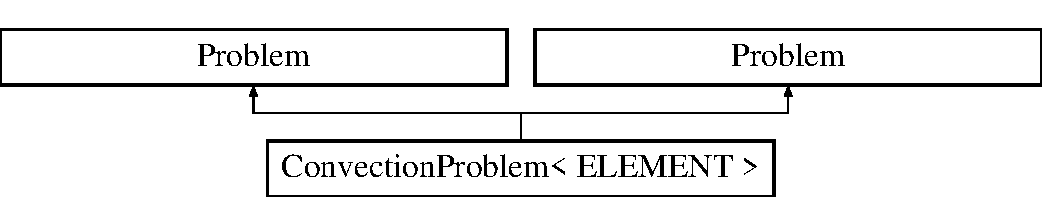
\includegraphics[height=2.000000cm]{classConvectionProblem}
\end{center}
\end{figure}
\subsection*{Public Member Functions}
\begin{DoxyCompactItemize}
\item 
\hyperlink{classConvectionProblem_a0c68c4c4b67d9fc8c9900fc895eed973}{Convection\+Problem} ()
\begin{DoxyCompactList}\small\item\em Constructor. \end{DoxyCompactList}\item 
\hyperlink{classConvectionProblem_a77c37355ba683b5b1ec11d096ce4d760}{$\sim$\+Convection\+Problem} ()
\begin{DoxyCompactList}\small\item\em Destructor. Empty. \end{DoxyCompactList}\item 
void \hyperlink{classConvectionProblem_a2fe48dd44ece8a0a69539ffcdce9ec11}{actions\+\_\+before\+\_\+newton\+\_\+solve} ()
\begin{DoxyCompactList}\small\item\em Update the problem specs before solve (empty) \end{DoxyCompactList}\item 
void \hyperlink{classConvectionProblem_a6b6c035decf5f1e2aa64b591563e5ae4}{actions\+\_\+after\+\_\+newton\+\_\+solve} ()
\begin{DoxyCompactList}\small\item\em Update the problem after solve (empty) \end{DoxyCompactList}\item 
void \hyperlink{classConvectionProblem_ac546cecdb98a75923d0a5af4b0a223a1}{actions\+\_\+before\+\_\+adapt} ()
\begin{DoxyCompactList}\small\item\em Actions before adapt\+:(empty) \end{DoxyCompactList}\item 
void \hyperlink{classConvectionProblem_a37c80882d173c02bfb3dfca924a4ec61}{actions\+\_\+before\+\_\+implicit\+\_\+timestep} ()
\begin{DoxyCompactList}\small\item\em Actions before the timestep (update the the time-\/dependent boundary conditions) \end{DoxyCompactList}\item 
void \hyperlink{classConvectionProblem_a5f4904e658a5888814e825ac060c8f71}{fix\+\_\+pressure} (const unsigned \&e, const unsigned \&pdof, const double \&pvalue)
\begin{DoxyCompactList}\small\item\em Fix pressure in element e at pressure dof pdof and set to pvalue. \end{DoxyCompactList}\item 
void \hyperlink{classConvectionProblem_ab7d9e5ac641ca08dd8b04c5eec179593}{doc\+\_\+solution} ()
\begin{DoxyCompactList}\small\item\em Doc the solution. \end{DoxyCompactList}\item 
void \hyperlink{classConvectionProblem_a605543718d51f7a77f75a46b48b543d7}{set\+\_\+boundary\+\_\+conditions} (const double \&time)
\begin{DoxyCompactList}\small\item\em Set the boundary conditions. \end{DoxyCompactList}\item 
Rectangular\+Quad\+Mesh$<$ E\+L\+E\+M\+E\+NT $>$ $\ast$ \hyperlink{classConvectionProblem_ad338a7928f0467b0fbad1b448c9a47c2}{mesh\+\_\+pt} ()
\begin{DoxyCompactList}\small\item\em Overloaded version of the problem\textquotesingle{}s access function to the mesh. Recasts the pointer to the base Mesh object to the actual mesh type. \end{DoxyCompactList}\item 
\hyperlink{classConvectionProblem_a16bb235fc46c4066134418a2323297c0}{Convection\+Problem} ()
\begin{DoxyCompactList}\small\item\em Constructor. \end{DoxyCompactList}\item 
\hyperlink{classConvectionProblem_a77c37355ba683b5b1ec11d096ce4d760}{$\sim$\+Convection\+Problem} ()
\begin{DoxyCompactList}\small\item\em Destructor. Empty. \end{DoxyCompactList}\item 
void \hyperlink{classConvectionProblem_a2fe48dd44ece8a0a69539ffcdce9ec11}{actions\+\_\+before\+\_\+newton\+\_\+solve} ()
\begin{DoxyCompactList}\small\item\em Update the problem specs before solve (empty) \end{DoxyCompactList}\item 
void \hyperlink{classConvectionProblem_a6b6c035decf5f1e2aa64b591563e5ae4}{actions\+\_\+after\+\_\+newton\+\_\+solve} ()
\begin{DoxyCompactList}\small\item\em Update the problem after solve (empty) \end{DoxyCompactList}\item 
void \hyperlink{classConvectionProblem_ac546cecdb98a75923d0a5af4b0a223a1}{actions\+\_\+before\+\_\+adapt} ()
\begin{DoxyCompactList}\small\item\em Actions before adapt\+:(empty) \end{DoxyCompactList}\item 
void \hyperlink{classConvectionProblem_a37c80882d173c02bfb3dfca924a4ec61}{actions\+\_\+before\+\_\+implicit\+\_\+timestep} ()
\begin{DoxyCompactList}\small\item\em Actions before the timestep (update the the time-\/dependent boundary conditions) \end{DoxyCompactList}\item 
void \hyperlink{classConvectionProblem_a5f4904e658a5888814e825ac060c8f71}{fix\+\_\+pressure} (const unsigned \&e, const unsigned \&pdof, const double \&pvalue)
\begin{DoxyCompactList}\small\item\em Fix pressure in element e at pressure dof pdof and set to pvalue. \end{DoxyCompactList}\item 
void \hyperlink{classConvectionProblem_a577e6ccb8106cbf3b2cede3bf4af7c24}{doc\+\_\+solution} ()
\begin{DoxyCompactList}\small\item\em Doc the solution. \end{DoxyCompactList}\item 
void \hyperlink{classConvectionProblem_a3b2e60458eead30fb143002a631683b7}{set\+\_\+boundary\+\_\+conditions} (const double \&time)
\begin{DoxyCompactList}\small\item\em Set the boundary conditions. \end{DoxyCompactList}\item 
Rectangular\+Quad\+Mesh$<$ N\+S\+T\+\_\+\+E\+L\+E\+M\+E\+NT $>$ $\ast$ \hyperlink{classConvectionProblem_a55cd8ffe7b4aa2165639dfdbe6006962}{nst\+\_\+mesh\+\_\+pt} ()
\begin{DoxyCompactList}\small\item\em Access function to the Navier-\/\+Stokes mesh. \end{DoxyCompactList}\item 
Rectangular\+Quad\+Mesh$<$ A\+D\+\_\+\+E\+L\+E\+M\+E\+NT $>$ $\ast$ \hyperlink{classConvectionProblem_a2c9c128da7f75c636ea04ac5643abf39}{adv\+\_\+diff\+\_\+mesh\+\_\+pt} ()
\begin{DoxyCompactList}\small\item\em Access function to the Advection-\/\+Diffusion mesh. \end{DoxyCompactList}\end{DoxyCompactItemize}
\subsection*{Protected Attributes}
\begin{DoxyCompactItemize}
\item 
Rectangular\+Quad\+Mesh$<$ N\+S\+T\+\_\+\+E\+L\+E\+M\+E\+NT $>$ $\ast$ \hyperlink{classConvectionProblem_a3bf695d1bd7b59b97aee57cfe66e4bcb}{Nst\+\_\+mesh\+\_\+pt}
\begin{DoxyCompactList}\small\item\em Mesh of Navier Stokes elements. \end{DoxyCompactList}\item 
Rectangular\+Quad\+Mesh$<$ A\+D\+\_\+\+E\+L\+E\+M\+E\+NT $>$ $\ast$ \hyperlink{classConvectionProblem_ac4dfae66888e0f70a71b10482d20bdc0}{Adv\+\_\+diff\+\_\+mesh\+\_\+pt}
\begin{DoxyCompactList}\small\item\em Mesh of advection diffusion elements. \end{DoxyCompactList}\end{DoxyCompactItemize}
\subsection*{Private Attributes}
\begin{DoxyCompactItemize}
\item 
Doc\+Info \hyperlink{classConvectionProblem_afc3f74343209527c9d30b5207d19983d}{Doc\+\_\+info}
\begin{DoxyCompactList}\small\item\em Doc\+Info object. \end{DoxyCompactList}\end{DoxyCompactItemize}


\subsection{Detailed Description}
\subsubsection*{template$<$class E\+L\+E\+M\+E\+NT$>$\newline
class Convection\+Problem$<$ E\+L\+E\+M\+E\+N\+T $>$}

2D Convection problem on rectangular domain, discretised with refineable elements. The specific type of element is specified via the template parameter.

2D Convection problem on two rectangular domains, discretised with Navier-\/\+Stokes and Advection-\/\+Diffusion elements. The specific type of elements is specified via the template parameters. 

Definition at line 79 of file boussinesq\+\_\+convection.\+cc.



\subsection{Constructor \& Destructor Documentation}
\mbox{\Hypertarget{classConvectionProblem_a0c68c4c4b67d9fc8c9900fc895eed973}\label{classConvectionProblem_a0c68c4c4b67d9fc8c9900fc895eed973}} 
\index{Convection\+Problem@{Convection\+Problem}!Convection\+Problem@{Convection\+Problem}}
\index{Convection\+Problem@{Convection\+Problem}!Convection\+Problem@{Convection\+Problem}}
\subsubsection{\texorpdfstring{Convection\+Problem()}{ConvectionProblem()}\hspace{0.1cm}{\footnotesize\ttfamily [1/2]}}
{\footnotesize\ttfamily template$<$class N\+S\+T\+\_\+\+E\+L\+E\+M\+E\+NT , class A\+D\+\_\+\+E\+L\+E\+M\+E\+NT $>$ \\
\hyperlink{classConvectionProblem}{Convection\+Problem}$<$ N\+S\+T\+\_\+\+E\+L\+E\+M\+E\+NT, A\+D\+\_\+\+E\+L\+E\+M\+E\+NT $>$\+::\hyperlink{classConvectionProblem}{Convection\+Problem} (\begin{DoxyParamCaption}{ }\end{DoxyParamCaption})}



Constructor. 

Constructor for convection problem. 

Definition at line 141 of file boussinesq\+\_\+convection.\+cc.



References Global\+\_\+\+Physical\+\_\+\+Variables\+::\+Direction\+\_\+of\+\_\+gravity(), Global\+\_\+\+Physical\+\_\+\+Variables\+::\+Inverse\+\_\+\+Prandtl, Global\+\_\+\+Physical\+\_\+\+Variables\+::\+Peclet, and Global\+\_\+\+Physical\+\_\+\+Variables\+::\+Rayleigh.

\mbox{\Hypertarget{classConvectionProblem_a77c37355ba683b5b1ec11d096ce4d760}\label{classConvectionProblem_a77c37355ba683b5b1ec11d096ce4d760}} 
\index{Convection\+Problem@{Convection\+Problem}!````~Convection\+Problem@{$\sim$\+Convection\+Problem}}
\index{````~Convection\+Problem@{$\sim$\+Convection\+Problem}!Convection\+Problem@{Convection\+Problem}}
\subsubsection{\texorpdfstring{$\sim$\+Convection\+Problem()}{~ConvectionProblem()}\hspace{0.1cm}{\footnotesize\ttfamily [1/2]}}
{\footnotesize\ttfamily template$<$class E\+L\+E\+M\+E\+NT$>$ \\
\hyperlink{classConvectionProblem}{Convection\+Problem}$<$ E\+L\+E\+M\+E\+NT $>$\+::$\sim$\hyperlink{classConvectionProblem}{Convection\+Problem} (\begin{DoxyParamCaption}{ }\end{DoxyParamCaption})\hspace{0.3cm}{\ttfamily [inline]}}



Destructor. Empty. 



Definition at line 88 of file boussinesq\+\_\+convection.\+cc.

\mbox{\Hypertarget{classConvectionProblem_a16bb235fc46c4066134418a2323297c0}\label{classConvectionProblem_a16bb235fc46c4066134418a2323297c0}} 
\index{Convection\+Problem@{Convection\+Problem}!Convection\+Problem@{Convection\+Problem}}
\index{Convection\+Problem@{Convection\+Problem}!Convection\+Problem@{Convection\+Problem}}
\subsubsection{\texorpdfstring{Convection\+Problem()}{ConvectionProblem()}\hspace{0.1cm}{\footnotesize\ttfamily [2/2]}}
{\footnotesize\ttfamily template$<$class E\+L\+E\+M\+E\+NT$>$ \\
\hyperlink{classConvectionProblem}{Convection\+Problem}$<$ E\+L\+E\+M\+E\+NT $>$\+::\hyperlink{classConvectionProblem}{Convection\+Problem} (\begin{DoxyParamCaption}{ }\end{DoxyParamCaption})}



Constructor. 

\mbox{\Hypertarget{classConvectionProblem_a77c37355ba683b5b1ec11d096ce4d760}\label{classConvectionProblem_a77c37355ba683b5b1ec11d096ce4d760}} 
\index{Convection\+Problem@{Convection\+Problem}!````~Convection\+Problem@{$\sim$\+Convection\+Problem}}
\index{````~Convection\+Problem@{$\sim$\+Convection\+Problem}!Convection\+Problem@{Convection\+Problem}}
\subsubsection{\texorpdfstring{$\sim$\+Convection\+Problem()}{~ConvectionProblem()}\hspace{0.1cm}{\footnotesize\ttfamily [2/2]}}
{\footnotesize\ttfamily template$<$class E\+L\+E\+M\+E\+NT$>$ \\
\hyperlink{classConvectionProblem}{Convection\+Problem}$<$ E\+L\+E\+M\+E\+NT $>$\+::$\sim$\hyperlink{classConvectionProblem}{Convection\+Problem} (\begin{DoxyParamCaption}{ }\end{DoxyParamCaption})\hspace{0.3cm}{\ttfamily [inline]}}



Destructor. Empty. 



Definition at line 88 of file multi\+\_\+domain\+\_\+boussinesq\+\_\+convection.\+cc.



\subsection{Member Function Documentation}
\mbox{\Hypertarget{classConvectionProblem_a6b6c035decf5f1e2aa64b591563e5ae4}\label{classConvectionProblem_a6b6c035decf5f1e2aa64b591563e5ae4}} 
\index{Convection\+Problem@{Convection\+Problem}!actions\+\_\+after\+\_\+newton\+\_\+solve@{actions\+\_\+after\+\_\+newton\+\_\+solve}}
\index{actions\+\_\+after\+\_\+newton\+\_\+solve@{actions\+\_\+after\+\_\+newton\+\_\+solve}!Convection\+Problem@{Convection\+Problem}}
\subsubsection{\texorpdfstring{actions\+\_\+after\+\_\+newton\+\_\+solve()}{actions\_after\_newton\_solve()}\hspace{0.1cm}{\footnotesize\ttfamily [1/2]}}
{\footnotesize\ttfamily template$<$class E\+L\+E\+M\+E\+NT$>$ \\
void \hyperlink{classConvectionProblem}{Convection\+Problem}$<$ E\+L\+E\+M\+E\+NT $>$\+::actions\+\_\+after\+\_\+newton\+\_\+solve (\begin{DoxyParamCaption}{ }\end{DoxyParamCaption})\hspace{0.3cm}{\ttfamily [inline]}}



Update the problem after solve (empty) 



Definition at line 94 of file boussinesq\+\_\+convection.\+cc.

\mbox{\Hypertarget{classConvectionProblem_a6b6c035decf5f1e2aa64b591563e5ae4}\label{classConvectionProblem_a6b6c035decf5f1e2aa64b591563e5ae4}} 
\index{Convection\+Problem@{Convection\+Problem}!actions\+\_\+after\+\_\+newton\+\_\+solve@{actions\+\_\+after\+\_\+newton\+\_\+solve}}
\index{actions\+\_\+after\+\_\+newton\+\_\+solve@{actions\+\_\+after\+\_\+newton\+\_\+solve}!Convection\+Problem@{Convection\+Problem}}
\subsubsection{\texorpdfstring{actions\+\_\+after\+\_\+newton\+\_\+solve()}{actions\_after\_newton\_solve()}\hspace{0.1cm}{\footnotesize\ttfamily [2/2]}}
{\footnotesize\ttfamily template$<$class E\+L\+E\+M\+E\+NT$>$ \\
void \hyperlink{classConvectionProblem}{Convection\+Problem}$<$ E\+L\+E\+M\+E\+NT $>$\+::actions\+\_\+after\+\_\+newton\+\_\+solve (\begin{DoxyParamCaption}{ }\end{DoxyParamCaption})\hspace{0.3cm}{\ttfamily [inline]}}



Update the problem after solve (empty) 



Definition at line 94 of file multi\+\_\+domain\+\_\+boussinesq\+\_\+convection.\+cc.

\mbox{\Hypertarget{classConvectionProblem_ac546cecdb98a75923d0a5af4b0a223a1}\label{classConvectionProblem_ac546cecdb98a75923d0a5af4b0a223a1}} 
\index{Convection\+Problem@{Convection\+Problem}!actions\+\_\+before\+\_\+adapt@{actions\+\_\+before\+\_\+adapt}}
\index{actions\+\_\+before\+\_\+adapt@{actions\+\_\+before\+\_\+adapt}!Convection\+Problem@{Convection\+Problem}}
\subsubsection{\texorpdfstring{actions\+\_\+before\+\_\+adapt()}{actions\_before\_adapt()}\hspace{0.1cm}{\footnotesize\ttfamily [1/2]}}
{\footnotesize\ttfamily template$<$class E\+L\+E\+M\+E\+NT$>$ \\
void \hyperlink{classConvectionProblem}{Convection\+Problem}$<$ E\+L\+E\+M\+E\+NT $>$\+::actions\+\_\+before\+\_\+adapt (\begin{DoxyParamCaption}{ }\end{DoxyParamCaption})\hspace{0.3cm}{\ttfamily [inline]}}



Actions before adapt\+:(empty) 



Definition at line 97 of file multi\+\_\+domain\+\_\+boussinesq\+\_\+convection.\+cc.

\mbox{\Hypertarget{classConvectionProblem_ac546cecdb98a75923d0a5af4b0a223a1}\label{classConvectionProblem_ac546cecdb98a75923d0a5af4b0a223a1}} 
\index{Convection\+Problem@{Convection\+Problem}!actions\+\_\+before\+\_\+adapt@{actions\+\_\+before\+\_\+adapt}}
\index{actions\+\_\+before\+\_\+adapt@{actions\+\_\+before\+\_\+adapt}!Convection\+Problem@{Convection\+Problem}}
\subsubsection{\texorpdfstring{actions\+\_\+before\+\_\+adapt()}{actions\_before\_adapt()}\hspace{0.1cm}{\footnotesize\ttfamily [2/2]}}
{\footnotesize\ttfamily template$<$class E\+L\+E\+M\+E\+NT$>$ \\
void \hyperlink{classConvectionProblem}{Convection\+Problem}$<$ E\+L\+E\+M\+E\+NT $>$\+::actions\+\_\+before\+\_\+adapt (\begin{DoxyParamCaption}{ }\end{DoxyParamCaption})\hspace{0.3cm}{\ttfamily [inline]}}



Actions before adapt\+:(empty) 



Definition at line 97 of file boussinesq\+\_\+convection.\+cc.

\mbox{\Hypertarget{classConvectionProblem_a37c80882d173c02bfb3dfca924a4ec61}\label{classConvectionProblem_a37c80882d173c02bfb3dfca924a4ec61}} 
\index{Convection\+Problem@{Convection\+Problem}!actions\+\_\+before\+\_\+implicit\+\_\+timestep@{actions\+\_\+before\+\_\+implicit\+\_\+timestep}}
\index{actions\+\_\+before\+\_\+implicit\+\_\+timestep@{actions\+\_\+before\+\_\+implicit\+\_\+timestep}!Convection\+Problem@{Convection\+Problem}}
\subsubsection{\texorpdfstring{actions\+\_\+before\+\_\+implicit\+\_\+timestep()}{actions\_before\_implicit\_timestep()}\hspace{0.1cm}{\footnotesize\ttfamily [1/2]}}
{\footnotesize\ttfamily template$<$class E\+L\+E\+M\+E\+NT$>$ \\
void \hyperlink{classConvectionProblem}{Convection\+Problem}$<$ E\+L\+E\+M\+E\+NT $>$\+::actions\+\_\+before\+\_\+implicit\+\_\+timestep (\begin{DoxyParamCaption}{ }\end{DoxyParamCaption})\hspace{0.3cm}{\ttfamily [inline]}}



Actions before the timestep (update the the time-\/dependent boundary conditions) 



Definition at line 101 of file boussinesq\+\_\+convection.\+cc.

\mbox{\Hypertarget{classConvectionProblem_a37c80882d173c02bfb3dfca924a4ec61}\label{classConvectionProblem_a37c80882d173c02bfb3dfca924a4ec61}} 
\index{Convection\+Problem@{Convection\+Problem}!actions\+\_\+before\+\_\+implicit\+\_\+timestep@{actions\+\_\+before\+\_\+implicit\+\_\+timestep}}
\index{actions\+\_\+before\+\_\+implicit\+\_\+timestep@{actions\+\_\+before\+\_\+implicit\+\_\+timestep}!Convection\+Problem@{Convection\+Problem}}
\subsubsection{\texorpdfstring{actions\+\_\+before\+\_\+implicit\+\_\+timestep()}{actions\_before\_implicit\_timestep()}\hspace{0.1cm}{\footnotesize\ttfamily [2/2]}}
{\footnotesize\ttfamily template$<$class E\+L\+E\+M\+E\+NT$>$ \\
void \hyperlink{classConvectionProblem}{Convection\+Problem}$<$ E\+L\+E\+M\+E\+NT $>$\+::actions\+\_\+before\+\_\+implicit\+\_\+timestep (\begin{DoxyParamCaption}{ }\end{DoxyParamCaption})\hspace{0.3cm}{\ttfamily [inline]}}



Actions before the timestep (update the the time-\/dependent boundary conditions) 



Definition at line 101 of file multi\+\_\+domain\+\_\+boussinesq\+\_\+convection.\+cc.

\mbox{\Hypertarget{classConvectionProblem_a2fe48dd44ece8a0a69539ffcdce9ec11}\label{classConvectionProblem_a2fe48dd44ece8a0a69539ffcdce9ec11}} 
\index{Convection\+Problem@{Convection\+Problem}!actions\+\_\+before\+\_\+newton\+\_\+solve@{actions\+\_\+before\+\_\+newton\+\_\+solve}}
\index{actions\+\_\+before\+\_\+newton\+\_\+solve@{actions\+\_\+before\+\_\+newton\+\_\+solve}!Convection\+Problem@{Convection\+Problem}}
\subsubsection{\texorpdfstring{actions\+\_\+before\+\_\+newton\+\_\+solve()}{actions\_before\_newton\_solve()}\hspace{0.1cm}{\footnotesize\ttfamily [1/2]}}
{\footnotesize\ttfamily template$<$class E\+L\+E\+M\+E\+NT$>$ \\
void \hyperlink{classConvectionProblem}{Convection\+Problem}$<$ E\+L\+E\+M\+E\+NT $>$\+::actions\+\_\+before\+\_\+newton\+\_\+solve (\begin{DoxyParamCaption}{ }\end{DoxyParamCaption})\hspace{0.3cm}{\ttfamily [inline]}}



Update the problem specs before solve (empty) 



Definition at line 91 of file boussinesq\+\_\+convection.\+cc.

\mbox{\Hypertarget{classConvectionProblem_a2fe48dd44ece8a0a69539ffcdce9ec11}\label{classConvectionProblem_a2fe48dd44ece8a0a69539ffcdce9ec11}} 
\index{Convection\+Problem@{Convection\+Problem}!actions\+\_\+before\+\_\+newton\+\_\+solve@{actions\+\_\+before\+\_\+newton\+\_\+solve}}
\index{actions\+\_\+before\+\_\+newton\+\_\+solve@{actions\+\_\+before\+\_\+newton\+\_\+solve}!Convection\+Problem@{Convection\+Problem}}
\subsubsection{\texorpdfstring{actions\+\_\+before\+\_\+newton\+\_\+solve()}{actions\_before\_newton\_solve()}\hspace{0.1cm}{\footnotesize\ttfamily [2/2]}}
{\footnotesize\ttfamily template$<$class E\+L\+E\+M\+E\+NT$>$ \\
void \hyperlink{classConvectionProblem}{Convection\+Problem}$<$ E\+L\+E\+M\+E\+NT $>$\+::actions\+\_\+before\+\_\+newton\+\_\+solve (\begin{DoxyParamCaption}{ }\end{DoxyParamCaption})\hspace{0.3cm}{\ttfamily [inline]}}



Update the problem specs before solve (empty) 



Definition at line 91 of file multi\+\_\+domain\+\_\+boussinesq\+\_\+convection.\+cc.

\mbox{\Hypertarget{classConvectionProblem_a2c9c128da7f75c636ea04ac5643abf39}\label{classConvectionProblem_a2c9c128da7f75c636ea04ac5643abf39}} 
\index{Convection\+Problem@{Convection\+Problem}!adv\+\_\+diff\+\_\+mesh\+\_\+pt@{adv\+\_\+diff\+\_\+mesh\+\_\+pt}}
\index{adv\+\_\+diff\+\_\+mesh\+\_\+pt@{adv\+\_\+diff\+\_\+mesh\+\_\+pt}!Convection\+Problem@{Convection\+Problem}}
\subsubsection{\texorpdfstring{adv\+\_\+diff\+\_\+mesh\+\_\+pt()}{adv\_diff\_mesh\_pt()}}
{\footnotesize\ttfamily template$<$class E\+L\+E\+M\+E\+NT$>$ \\
Rectangular\+Quad\+Mesh$<$A\+D\+\_\+\+E\+L\+E\+M\+E\+NT$>$$\ast$ \hyperlink{classConvectionProblem}{Convection\+Problem}$<$ E\+L\+E\+M\+E\+NT $>$\+::adv\+\_\+diff\+\_\+mesh\+\_\+pt (\begin{DoxyParamCaption}{ }\end{DoxyParamCaption})\hspace{0.3cm}{\ttfamily [inline]}}



Access function to the Advection-\/\+Diffusion mesh. 



Definition at line 128 of file multi\+\_\+domain\+\_\+boussinesq\+\_\+convection.\+cc.

\mbox{\Hypertarget{classConvectionProblem_ab7d9e5ac641ca08dd8b04c5eec179593}\label{classConvectionProblem_ab7d9e5ac641ca08dd8b04c5eec179593}} 
\index{Convection\+Problem@{Convection\+Problem}!doc\+\_\+solution@{doc\+\_\+solution}}
\index{doc\+\_\+solution@{doc\+\_\+solution}!Convection\+Problem@{Convection\+Problem}}
\subsubsection{\texorpdfstring{doc\+\_\+solution()}{doc\_solution()}\hspace{0.1cm}{\footnotesize\ttfamily [1/2]}}
{\footnotesize\ttfamily template$<$class N\+S\+T\+\_\+\+E\+L\+E\+M\+E\+NT , class A\+D\+\_\+\+E\+L\+E\+M\+E\+NT $>$ \\
void \hyperlink{classConvectionProblem}{Convection\+Problem}$<$ N\+S\+T\+\_\+\+E\+L\+E\+M\+E\+NT, A\+D\+\_\+\+E\+L\+E\+M\+E\+NT $>$\+::doc\+\_\+solution (\begin{DoxyParamCaption}{ }\end{DoxyParamCaption})}



Doc the solution. 



Definition at line 294 of file boussinesq\+\_\+convection.\+cc.



Referenced by main().

\mbox{\Hypertarget{classConvectionProblem_a577e6ccb8106cbf3b2cede3bf4af7c24}\label{classConvectionProblem_a577e6ccb8106cbf3b2cede3bf4af7c24}} 
\index{Convection\+Problem@{Convection\+Problem}!doc\+\_\+solution@{doc\+\_\+solution}}
\index{doc\+\_\+solution@{doc\+\_\+solution}!Convection\+Problem@{Convection\+Problem}}
\subsubsection{\texorpdfstring{doc\+\_\+solution()}{doc\_solution()}\hspace{0.1cm}{\footnotesize\ttfamily [2/2]}}
{\footnotesize\ttfamily template$<$class E\+L\+E\+M\+E\+NT$>$ \\
void \hyperlink{classConvectionProblem}{Convection\+Problem}$<$ E\+L\+E\+M\+E\+NT $>$\+::doc\+\_\+solution (\begin{DoxyParamCaption}{ }\end{DoxyParamCaption})}



Doc the solution. 

\mbox{\Hypertarget{classConvectionProblem_a5f4904e658a5888814e825ac060c8f71}\label{classConvectionProblem_a5f4904e658a5888814e825ac060c8f71}} 
\index{Convection\+Problem@{Convection\+Problem}!fix\+\_\+pressure@{fix\+\_\+pressure}}
\index{fix\+\_\+pressure@{fix\+\_\+pressure}!Convection\+Problem@{Convection\+Problem}}
\subsubsection{\texorpdfstring{fix\+\_\+pressure()}{fix\_pressure()}\hspace{0.1cm}{\footnotesize\ttfamily [1/2]}}
{\footnotesize\ttfamily template$<$class E\+L\+E\+M\+E\+NT$>$ \\
void \hyperlink{classConvectionProblem}{Convection\+Problem}$<$ E\+L\+E\+M\+E\+NT $>$\+::fix\+\_\+pressure (\begin{DoxyParamCaption}\item[{const unsigned \&}]{e,  }\item[{const unsigned \&}]{pdof,  }\item[{const double \&}]{pvalue }\end{DoxyParamCaption})\hspace{0.3cm}{\ttfamily [inline]}}



Fix pressure in element e at pressure dof pdof and set to pvalue. 



Definition at line 107 of file boussinesq\+\_\+convection.\+cc.

\mbox{\Hypertarget{classConvectionProblem_a5f4904e658a5888814e825ac060c8f71}\label{classConvectionProblem_a5f4904e658a5888814e825ac060c8f71}} 
\index{Convection\+Problem@{Convection\+Problem}!fix\+\_\+pressure@{fix\+\_\+pressure}}
\index{fix\+\_\+pressure@{fix\+\_\+pressure}!Convection\+Problem@{Convection\+Problem}}
\subsubsection{\texorpdfstring{fix\+\_\+pressure()}{fix\_pressure()}\hspace{0.1cm}{\footnotesize\ttfamily [2/2]}}
{\footnotesize\ttfamily template$<$class E\+L\+E\+M\+E\+NT$>$ \\
void \hyperlink{classConvectionProblem}{Convection\+Problem}$<$ E\+L\+E\+M\+E\+NT $>$\+::fix\+\_\+pressure (\begin{DoxyParamCaption}\item[{const unsigned \&}]{e,  }\item[{const unsigned \&}]{pdof,  }\item[{const double \&}]{pvalue }\end{DoxyParamCaption})\hspace{0.3cm}{\ttfamily [inline]}}



Fix pressure in element e at pressure dof pdof and set to pvalue. 



Definition at line 107 of file multi\+\_\+domain\+\_\+boussinesq\+\_\+convection.\+cc.

\mbox{\Hypertarget{classConvectionProblem_ad338a7928f0467b0fbad1b448c9a47c2}\label{classConvectionProblem_ad338a7928f0467b0fbad1b448c9a47c2}} 
\index{Convection\+Problem@{Convection\+Problem}!mesh\+\_\+pt@{mesh\+\_\+pt}}
\index{mesh\+\_\+pt@{mesh\+\_\+pt}!Convection\+Problem@{Convection\+Problem}}
\subsubsection{\texorpdfstring{mesh\+\_\+pt()}{mesh\_pt()}}
{\footnotesize\ttfamily template$<$class E\+L\+E\+M\+E\+NT$>$ \\
Rectangular\+Quad\+Mesh$<$E\+L\+E\+M\+E\+NT$>$$\ast$ \hyperlink{classConvectionProblem}{Convection\+Problem}$<$ E\+L\+E\+M\+E\+NT $>$\+::mesh\+\_\+pt (\begin{DoxyParamCaption}{ }\end{DoxyParamCaption})\hspace{0.3cm}{\ttfamily [inline]}}



Overloaded version of the problem\textquotesingle{}s access function to the mesh. Recasts the pointer to the base Mesh object to the actual mesh type. 



Definition at line 124 of file boussinesq\+\_\+convection.\+cc.

\mbox{\Hypertarget{classConvectionProblem_a55cd8ffe7b4aa2165639dfdbe6006962}\label{classConvectionProblem_a55cd8ffe7b4aa2165639dfdbe6006962}} 
\index{Convection\+Problem@{Convection\+Problem}!nst\+\_\+mesh\+\_\+pt@{nst\+\_\+mesh\+\_\+pt}}
\index{nst\+\_\+mesh\+\_\+pt@{nst\+\_\+mesh\+\_\+pt}!Convection\+Problem@{Convection\+Problem}}
\subsubsection{\texorpdfstring{nst\+\_\+mesh\+\_\+pt()}{nst\_mesh\_pt()}}
{\footnotesize\ttfamily template$<$class E\+L\+E\+M\+E\+NT$>$ \\
Rectangular\+Quad\+Mesh$<$N\+S\+T\+\_\+\+E\+L\+E\+M\+E\+NT$>$$\ast$ \hyperlink{classConvectionProblem}{Convection\+Problem}$<$ E\+L\+E\+M\+E\+NT $>$\+::nst\+\_\+mesh\+\_\+pt (\begin{DoxyParamCaption}{ }\end{DoxyParamCaption})\hspace{0.3cm}{\ttfamily [inline]}}



Access function to the Navier-\/\+Stokes mesh. 



Definition at line 122 of file multi\+\_\+domain\+\_\+boussinesq\+\_\+convection.\+cc.

\mbox{\Hypertarget{classConvectionProblem_a3b2e60458eead30fb143002a631683b7}\label{classConvectionProblem_a3b2e60458eead30fb143002a631683b7}} 
\index{Convection\+Problem@{Convection\+Problem}!set\+\_\+boundary\+\_\+conditions@{set\+\_\+boundary\+\_\+conditions}}
\index{set\+\_\+boundary\+\_\+conditions@{set\+\_\+boundary\+\_\+conditions}!Convection\+Problem@{Convection\+Problem}}
\subsubsection{\texorpdfstring{set\+\_\+boundary\+\_\+conditions()}{set\_boundary\_conditions()}\hspace{0.1cm}{\footnotesize\ttfamily [1/2]}}
{\footnotesize\ttfamily template$<$class E\+L\+E\+M\+E\+NT$>$ \\
void \hyperlink{classConvectionProblem}{Convection\+Problem}$<$ E\+L\+E\+M\+E\+NT $>$\+::set\+\_\+boundary\+\_\+conditions (\begin{DoxyParamCaption}\item[{const double \&}]{time }\end{DoxyParamCaption})}



Set the boundary conditions. 

\mbox{\Hypertarget{classConvectionProblem_a605543718d51f7a77f75a46b48b543d7}\label{classConvectionProblem_a605543718d51f7a77f75a46b48b543d7}} 
\index{Convection\+Problem@{Convection\+Problem}!set\+\_\+boundary\+\_\+conditions@{set\+\_\+boundary\+\_\+conditions}}
\index{set\+\_\+boundary\+\_\+conditions@{set\+\_\+boundary\+\_\+conditions}!Convection\+Problem@{Convection\+Problem}}
\subsubsection{\texorpdfstring{set\+\_\+boundary\+\_\+conditions()}{set\_boundary\_conditions()}\hspace{0.1cm}{\footnotesize\ttfamily [2/2]}}
{\footnotesize\ttfamily template$<$class N\+S\+T\+\_\+\+E\+L\+E\+M\+E\+NT , class A\+D\+\_\+\+E\+L\+E\+M\+E\+NT $>$ \\
void \hyperlink{classConvectionProblem}{Convection\+Problem}$<$ N\+S\+T\+\_\+\+E\+L\+E\+M\+E\+NT, A\+D\+\_\+\+E\+L\+E\+M\+E\+NT $>$\+::set\+\_\+boundary\+\_\+conditions (\begin{DoxyParamCaption}\item[{const double \&}]{time }\end{DoxyParamCaption})}



Set the boundary conditions. 

Set the boundary conditions as a function of continuous time 

Definition at line 241 of file boussinesq\+\_\+convection.\+cc.



Referenced by main().



\subsection{Member Data Documentation}
\mbox{\Hypertarget{classConvectionProblem_ac4dfae66888e0f70a71b10482d20bdc0}\label{classConvectionProblem_ac4dfae66888e0f70a71b10482d20bdc0}} 
\index{Convection\+Problem@{Convection\+Problem}!Adv\+\_\+diff\+\_\+mesh\+\_\+pt@{Adv\+\_\+diff\+\_\+mesh\+\_\+pt}}
\index{Adv\+\_\+diff\+\_\+mesh\+\_\+pt@{Adv\+\_\+diff\+\_\+mesh\+\_\+pt}!Convection\+Problem@{Convection\+Problem}}
\subsubsection{\texorpdfstring{Adv\+\_\+diff\+\_\+mesh\+\_\+pt}{Adv\_diff\_mesh\_pt}}
{\footnotesize\ttfamily template$<$class E\+L\+E\+M\+E\+NT$>$ \\
Rectangular\+Quad\+Mesh$<$A\+D\+\_\+\+E\+L\+E\+M\+E\+NT$>$$\ast$ \hyperlink{classConvectionProblem}{Convection\+Problem}$<$ E\+L\+E\+M\+E\+NT $>$\+::Adv\+\_\+diff\+\_\+mesh\+\_\+pt\hspace{0.3cm}{\ttfamily [protected]}}



Mesh of advection diffusion elements. 



Definition at line 144 of file multi\+\_\+domain\+\_\+boussinesq\+\_\+convection.\+cc.

\mbox{\Hypertarget{classConvectionProblem_afc3f74343209527c9d30b5207d19983d}\label{classConvectionProblem_afc3f74343209527c9d30b5207d19983d}} 
\index{Convection\+Problem@{Convection\+Problem}!Doc\+\_\+info@{Doc\+\_\+info}}
\index{Doc\+\_\+info@{Doc\+\_\+info}!Convection\+Problem@{Convection\+Problem}}
\subsubsection{\texorpdfstring{Doc\+\_\+info}{Doc\_info}}
{\footnotesize\ttfamily template$<$class E\+L\+E\+M\+E\+NT$>$ \\
Doc\+Info \hyperlink{classConvectionProblem}{Convection\+Problem}$<$ E\+L\+E\+M\+E\+NT $>$\+::Doc\+\_\+info\hspace{0.3cm}{\ttfamily [private]}}



Doc\+Info object. 



Definition at line 133 of file boussinesq\+\_\+convection.\+cc.

\mbox{\Hypertarget{classConvectionProblem_a3bf695d1bd7b59b97aee57cfe66e4bcb}\label{classConvectionProblem_a3bf695d1bd7b59b97aee57cfe66e4bcb}} 
\index{Convection\+Problem@{Convection\+Problem}!Nst\+\_\+mesh\+\_\+pt@{Nst\+\_\+mesh\+\_\+pt}}
\index{Nst\+\_\+mesh\+\_\+pt@{Nst\+\_\+mesh\+\_\+pt}!Convection\+Problem@{Convection\+Problem}}
\subsubsection{\texorpdfstring{Nst\+\_\+mesh\+\_\+pt}{Nst\_mesh\_pt}}
{\footnotesize\ttfamily template$<$class E\+L\+E\+M\+E\+NT$>$ \\
Rectangular\+Quad\+Mesh$<$N\+S\+T\+\_\+\+E\+L\+E\+M\+E\+NT$>$$\ast$ \hyperlink{classConvectionProblem}{Convection\+Problem}$<$ E\+L\+E\+M\+E\+NT $>$\+::Nst\+\_\+mesh\+\_\+pt\hspace{0.3cm}{\ttfamily [protected]}}



Mesh of Navier Stokes elements. 



Definition at line 141 of file multi\+\_\+domain\+\_\+boussinesq\+\_\+convection.\+cc.



The documentation for this class was generated from the following files\+:\begin{DoxyCompactItemize}
\item 
\hyperlink{boussinesq__convection_8cc}{boussinesq\+\_\+convection.\+cc}\item 
\hyperlink{multi__domain__boussinesq__convection_8cc}{multi\+\_\+domain\+\_\+boussinesq\+\_\+convection.\+cc}\end{DoxyCompactItemize}

\hypertarget{classoomph_1_1FaceGeometry_3_01BuoyantQCrouzeixRaviartElement_3_01DIM_01_4_01_4}{}\section{oomph\+:\+:Face\+Geometry$<$ Buoyant\+Q\+Crouzeix\+Raviart\+Element$<$ D\+IM $>$ $>$ Class Template Reference}
\label{classoomph_1_1FaceGeometry_3_01BuoyantQCrouzeixRaviartElement_3_01DIM_01_4_01_4}\index{oomph\+::\+Face\+Geometry$<$ Buoyant\+Q\+Crouzeix\+Raviart\+Element$<$ D\+I\+M $>$ $>$@{oomph\+::\+Face\+Geometry$<$ Buoyant\+Q\+Crouzeix\+Raviart\+Element$<$ D\+I\+M $>$ $>$}}


Face geometry of the 2D Buoyant Crouzeix\+\_\+\+Raviart elements.  




{\ttfamily \#include $<$boussinesq\+\_\+elements.\+h$>$}

Inheritance diagram for oomph\+:\+:Face\+Geometry$<$ Buoyant\+Q\+Crouzeix\+Raviart\+Element$<$ D\+IM $>$ $>$\+:\begin{figure}[H]
\begin{center}
\leavevmode
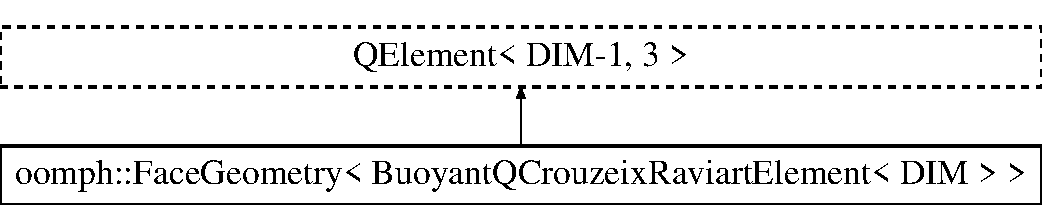
\includegraphics[height=2.000000cm]{classoomph_1_1FaceGeometry_3_01BuoyantQCrouzeixRaviartElement_3_01DIM_01_4_01_4}
\end{center}
\end{figure}
\subsection*{Public Member Functions}
\begin{DoxyCompactItemize}
\item 
\hyperlink{classoomph_1_1FaceGeometry_3_01BuoyantQCrouzeixRaviartElement_3_01DIM_01_4_01_4_a3cda0efe7f320d2eee2d7af336fa51fa}{Face\+Geometry} ()
\end{DoxyCompactItemize}


\subsection{Detailed Description}
\subsubsection*{template$<$unsigned int D\+IM$>$\newline
class oomph\+::\+Face\+Geometry$<$ Buoyant\+Q\+Crouzeix\+Raviart\+Element$<$ D\+I\+M $>$ $>$}

Face geometry of the 2D Buoyant Crouzeix\+\_\+\+Raviart elements. 

Definition at line 713 of file boussinesq\+\_\+elements.\+h.



\subsection{Constructor \& Destructor Documentation}
\mbox{\Hypertarget{classoomph_1_1FaceGeometry_3_01BuoyantQCrouzeixRaviartElement_3_01DIM_01_4_01_4_a3cda0efe7f320d2eee2d7af336fa51fa}\label{classoomph_1_1FaceGeometry_3_01BuoyantQCrouzeixRaviartElement_3_01DIM_01_4_01_4_a3cda0efe7f320d2eee2d7af336fa51fa}} 
\index{oomph\+::\+Face\+Geometry$<$ Buoyant\+Q\+Crouzeix\+Raviart\+Element$<$ D\+I\+M $>$ $>$@{oomph\+::\+Face\+Geometry$<$ Buoyant\+Q\+Crouzeix\+Raviart\+Element$<$ D\+I\+M $>$ $>$}!Face\+Geometry@{Face\+Geometry}}
\index{Face\+Geometry@{Face\+Geometry}!oomph\+::\+Face\+Geometry$<$ Buoyant\+Q\+Crouzeix\+Raviart\+Element$<$ D\+I\+M $>$ $>$@{oomph\+::\+Face\+Geometry$<$ Buoyant\+Q\+Crouzeix\+Raviart\+Element$<$ D\+I\+M $>$ $>$}}
\subsubsection{\texorpdfstring{Face\+Geometry()}{FaceGeometry()}}
{\footnotesize\ttfamily template$<$unsigned int D\+IM$>$ \\
\hyperlink{classoomph_1_1FaceGeometry}{oomph\+::\+Face\+Geometry}$<$ \hyperlink{classoomph_1_1BuoyantQCrouzeixRaviartElement}{Buoyant\+Q\+Crouzeix\+Raviart\+Element}$<$ D\+IM $>$ $>$\+::\hyperlink{classoomph_1_1FaceGeometry}{Face\+Geometry} (\begin{DoxyParamCaption}{ }\end{DoxyParamCaption})\hspace{0.3cm}{\ttfamily [inline]}}



Definition at line 717 of file boussinesq\+\_\+elements.\+h.



The documentation for this class was generated from the following file\+:\begin{DoxyCompactItemize}
\item 
\hyperlink{boussinesq__elements_8h}{boussinesq\+\_\+elements.\+h}\end{DoxyCompactItemize}

\hypertarget{classoomph_1_1FaceGeometry_3_01FaceGeometry_3_01BuoyantQCrouzeixRaviartElement_3_012_01_4_01_4_01_4}{}\section{oomph\+:\+:Face\+Geometry$<$ Face\+Geometry$<$ Buoyant\+Q\+Crouzeix\+Raviart\+Element$<$ 2 $>$ $>$ $>$ Class Template Reference}
\label{classoomph_1_1FaceGeometry_3_01FaceGeometry_3_01BuoyantQCrouzeixRaviartElement_3_012_01_4_01_4_01_4}\index{oomph\+::\+Face\+Geometry$<$ Face\+Geometry$<$ Buoyant\+Q\+Crouzeix\+Raviart\+Element$<$ 2 $>$ $>$ $>$@{oomph\+::\+Face\+Geometry$<$ Face\+Geometry$<$ Buoyant\+Q\+Crouzeix\+Raviart\+Element$<$ 2 $>$ $>$ $>$}}


Face geometry of the Face geometry of 2D Buoyant Crouzeix\+\_\+\+Raviart elements.  




{\ttfamily \#include $<$boussinesq\+\_\+elements.\+h$>$}

Inheritance diagram for oomph\+:\+:Face\+Geometry$<$ Face\+Geometry$<$ Buoyant\+Q\+Crouzeix\+Raviart\+Element$<$ 2 $>$ $>$ $>$\+:\begin{figure}[H]
\begin{center}
\leavevmode
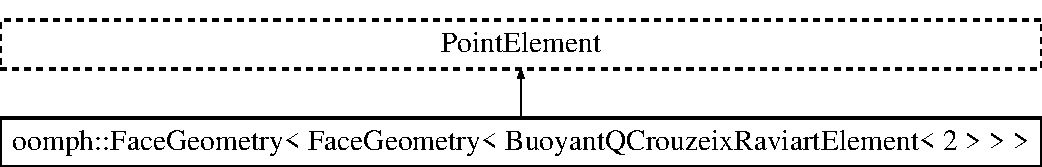
\includegraphics[height=2.000000cm]{classoomph_1_1FaceGeometry_3_01FaceGeometry_3_01BuoyantQCrouzeixRaviartElement_3_012_01_4_01_4_01_4}
\end{center}
\end{figure}
\subsection*{Public Member Functions}
\begin{DoxyCompactItemize}
\item 
\hyperlink{classoomph_1_1FaceGeometry_3_01FaceGeometry_3_01BuoyantQCrouzeixRaviartElement_3_012_01_4_01_4_01_4_af5838040ad0b4b6d95435e65abc2888c}{Face\+Geometry} ()
\end{DoxyCompactItemize}


\subsection{Detailed Description}
\subsubsection*{template$<$$>$\newline
class oomph\+::\+Face\+Geometry$<$ Face\+Geometry$<$ Buoyant\+Q\+Crouzeix\+Raviart\+Element$<$ 2 $>$ $>$ $>$}

Face geometry of the Face geometry of 2D Buoyant Crouzeix\+\_\+\+Raviart elements. 

Definition at line 724 of file boussinesq\+\_\+elements.\+h.



\subsection{Constructor \& Destructor Documentation}
\mbox{\Hypertarget{classoomph_1_1FaceGeometry_3_01FaceGeometry_3_01BuoyantQCrouzeixRaviartElement_3_012_01_4_01_4_01_4_af5838040ad0b4b6d95435e65abc2888c}\label{classoomph_1_1FaceGeometry_3_01FaceGeometry_3_01BuoyantQCrouzeixRaviartElement_3_012_01_4_01_4_01_4_af5838040ad0b4b6d95435e65abc2888c}} 
\index{oomph\+::\+Face\+Geometry$<$ Face\+Geometry$<$ Buoyant\+Q\+Crouzeix\+Raviart\+Element$<$ 2 $>$ $>$ $>$@{oomph\+::\+Face\+Geometry$<$ Face\+Geometry$<$ Buoyant\+Q\+Crouzeix\+Raviart\+Element$<$ 2 $>$ $>$ $>$}!Face\+Geometry@{Face\+Geometry}}
\index{Face\+Geometry@{Face\+Geometry}!oomph\+::\+Face\+Geometry$<$ Face\+Geometry$<$ Buoyant\+Q\+Crouzeix\+Raviart\+Element$<$ 2 $>$ $>$ $>$@{oomph\+::\+Face\+Geometry$<$ Face\+Geometry$<$ Buoyant\+Q\+Crouzeix\+Raviart\+Element$<$ 2 $>$ $>$ $>$}}
\subsubsection{\texorpdfstring{Face\+Geometry()}{FaceGeometry()}}
{\footnotesize\ttfamily oomph\+::\+Face\+Geometry$<$ Face\+Geometry$<$ \hyperlink{classoomph_1_1BuoyantQCrouzeixRaviartElement}{Buoyant\+Q\+Crouzeix\+Raviart\+Element}$<$ 2 $>$ $>$ $>$\+::Face\+Geometry (\begin{DoxyParamCaption}{ }\end{DoxyParamCaption})\hspace{0.3cm}{\ttfamily [inline]}}



Definition at line 728 of file boussinesq\+\_\+elements.\+h.



The documentation for this class was generated from the following file\+:\begin{DoxyCompactItemize}
\item 
\hyperlink{boussinesq__elements_8h}{boussinesq\+\_\+elements.\+h}\end{DoxyCompactItemize}

\hypertarget{classoomph_1_1FaceGeometry_3_01FaceGeometry_3_01NavierStokesBoussinesqElement_3_01NST__ELEMENT_00_01AD__ELEMENT_01_4_01_4_01_4}{}\section{oomph\+:\+:Face\+Geometry$<$ Face\+Geometry$<$ Navier\+Stokes\+Boussinesq\+Element$<$ N\+S\+T\+\_\+\+E\+L\+E\+M\+E\+NT, A\+D\+\_\+\+E\+L\+E\+M\+E\+NT $>$ $>$ $>$ Class Template Reference}
\label{classoomph_1_1FaceGeometry_3_01FaceGeometry_3_01NavierStokesBoussinesqElement_3_01NST__ELEMENT_00_01AD__ELEMENT_01_4_01_4_01_4}\index{oomph\+::\+Face\+Geometry$<$ Face\+Geometry$<$ Navier\+Stokes\+Boussinesq\+Element$<$ N\+S\+T\+\_\+\+E\+L\+E\+M\+E\+N\+T, A\+D\+\_\+\+E\+L\+E\+M\+E\+N\+T $>$ $>$ $>$@{oomph\+::\+Face\+Geometry$<$ Face\+Geometry$<$ Navier\+Stokes\+Boussinesq\+Element$<$ N\+S\+T\+\_\+\+E\+L\+E\+M\+E\+N\+T, A\+D\+\_\+\+E\+L\+E\+M\+E\+N\+T $>$ $>$ $>$}}


Explicit definition of the face geometry of these elements.  




{\ttfamily \#include $<$multi\+\_\+domain\+\_\+boussinesq\+\_\+elements.\+h$>$}

Inheritance diagram for oomph\+:\+:Face\+Geometry$<$ Face\+Geometry$<$ Navier\+Stokes\+Boussinesq\+Element$<$ N\+S\+T\+\_\+\+E\+L\+E\+M\+E\+NT, A\+D\+\_\+\+E\+L\+E\+M\+E\+NT $>$ $>$ $>$\+:\begin{figure}[H]
\begin{center}
\leavevmode
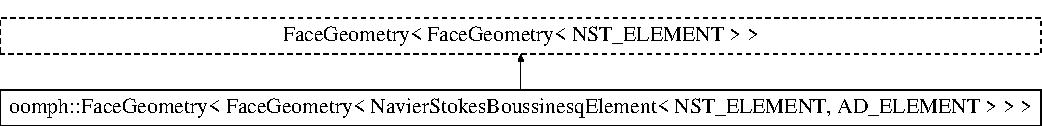
\includegraphics[height=1.686747cm]{classoomph_1_1FaceGeometry_3_01FaceGeometry_3_01NavierStokesBoussinesqElement_3_01NST__ELEMENT_00_01AD__ELEMENT_01_4_01_4_01_4}
\end{center}
\end{figure}
\subsection*{Public Member Functions}
\begin{DoxyCompactItemize}
\item 
\hyperlink{classoomph_1_1FaceGeometry_3_01FaceGeometry_3_01NavierStokesBoussinesqElement_3_01NST__ELEMENT_00_01AD__ELEMENT_01_4_01_4_01_4_a640fe9a3ce4f84f9d581bf56668dac63}{Face\+Geometry} ()
\begin{DoxyCompactList}\small\item\em Constructor calls the constructor of the N\+S\+T\+\_\+\+E\+L\+E\+M\+E\+NT (Only the Intel compiler seems to need this!) \end{DoxyCompactList}\end{DoxyCompactItemize}


\subsection{Detailed Description}
\subsubsection*{template$<$class N\+S\+T\+\_\+\+E\+L\+E\+M\+E\+NT, class A\+D\+\_\+\+E\+L\+E\+M\+E\+NT$>$\newline
class oomph\+::\+Face\+Geometry$<$ Face\+Geometry$<$ Navier\+Stokes\+Boussinesq\+Element$<$ N\+S\+T\+\_\+\+E\+L\+E\+M\+E\+N\+T, A\+D\+\_\+\+E\+L\+E\+M\+E\+N\+T $>$ $>$ $>$}

Explicit definition of the face geometry of these elements. 

Definition at line 1030 of file multi\+\_\+domain\+\_\+boussinesq\+\_\+elements.\+h.



\subsection{Constructor \& Destructor Documentation}
\mbox{\Hypertarget{classoomph_1_1FaceGeometry_3_01FaceGeometry_3_01NavierStokesBoussinesqElement_3_01NST__ELEMENT_00_01AD__ELEMENT_01_4_01_4_01_4_a640fe9a3ce4f84f9d581bf56668dac63}\label{classoomph_1_1FaceGeometry_3_01FaceGeometry_3_01NavierStokesBoussinesqElement_3_01NST__ELEMENT_00_01AD__ELEMENT_01_4_01_4_01_4_a640fe9a3ce4f84f9d581bf56668dac63}} 
\index{oomph\+::\+Face\+Geometry$<$ Face\+Geometry$<$ Navier\+Stokes\+Boussinesq\+Element$<$ N\+S\+T\+\_\+\+E\+L\+E\+M\+E\+N\+T, A\+D\+\_\+\+E\+L\+E\+M\+E\+N\+T $>$ $>$ $>$@{oomph\+::\+Face\+Geometry$<$ Face\+Geometry$<$ Navier\+Stokes\+Boussinesq\+Element$<$ N\+S\+T\+\_\+\+E\+L\+E\+M\+E\+N\+T, A\+D\+\_\+\+E\+L\+E\+M\+E\+N\+T $>$ $>$ $>$}!Face\+Geometry@{Face\+Geometry}}
\index{Face\+Geometry@{Face\+Geometry}!oomph\+::\+Face\+Geometry$<$ Face\+Geometry$<$ Navier\+Stokes\+Boussinesq\+Element$<$ N\+S\+T\+\_\+\+E\+L\+E\+M\+E\+N\+T, A\+D\+\_\+\+E\+L\+E\+M\+E\+N\+T $>$ $>$ $>$@{oomph\+::\+Face\+Geometry$<$ Face\+Geometry$<$ Navier\+Stokes\+Boussinesq\+Element$<$ N\+S\+T\+\_\+\+E\+L\+E\+M\+E\+N\+T, A\+D\+\_\+\+E\+L\+E\+M\+E\+N\+T $>$ $>$ $>$}}
\subsubsection{\texorpdfstring{Face\+Geometry()}{FaceGeometry()}}
{\footnotesize\ttfamily template$<$class N\+S\+T\+\_\+\+E\+L\+E\+M\+E\+NT , class A\+D\+\_\+\+E\+L\+E\+M\+E\+NT $>$ \\
oomph\+::\+Face\+Geometry$<$ Face\+Geometry$<$ \hyperlink{classoomph_1_1NavierStokesBoussinesqElement}{Navier\+Stokes\+Boussinesq\+Element}$<$ N\+S\+T\+\_\+\+E\+L\+E\+M\+E\+NT, A\+D\+\_\+\+E\+L\+E\+M\+E\+NT $>$ $>$ $>$\+::Face\+Geometry (\begin{DoxyParamCaption}{ }\end{DoxyParamCaption})\hspace{0.3cm}{\ttfamily [inline]}}



Constructor calls the constructor of the N\+S\+T\+\_\+\+E\+L\+E\+M\+E\+NT (Only the Intel compiler seems to need this!) 



Definition at line 1037 of file multi\+\_\+domain\+\_\+boussinesq\+\_\+elements.\+h.



The documentation for this class was generated from the following file\+:\begin{DoxyCompactItemize}
\item 
\hyperlink{multi__domain__boussinesq__elements_8h}{multi\+\_\+domain\+\_\+boussinesq\+\_\+elements.\+h}\end{DoxyCompactItemize}

\hypertarget{classoomph_1_1FaceGeometry_3_01NavierStokesBoussinesqElement_3_01NST__ELEMENT_00_01AD__ELEMENT_01_4_01_4}{}\section{oomph\+:\+:Face\+Geometry$<$ Navier\+Stokes\+Boussinesq\+Element$<$ N\+S\+T\+\_\+\+E\+L\+E\+M\+E\+NT, A\+D\+\_\+\+E\+L\+E\+M\+E\+NT $>$ $>$ Class Template Reference}
\label{classoomph_1_1FaceGeometry_3_01NavierStokesBoussinesqElement_3_01NST__ELEMENT_00_01AD__ELEMENT_01_4_01_4}\index{oomph\+::\+Face\+Geometry$<$ Navier\+Stokes\+Boussinesq\+Element$<$ N\+S\+T\+\_\+\+E\+L\+E\+M\+E\+N\+T, A\+D\+\_\+\+E\+L\+E\+M\+E\+N\+T $>$ $>$@{oomph\+::\+Face\+Geometry$<$ Navier\+Stokes\+Boussinesq\+Element$<$ N\+S\+T\+\_\+\+E\+L\+E\+M\+E\+N\+T, A\+D\+\_\+\+E\+L\+E\+M\+E\+N\+T $>$ $>$}}


Explicit definition of the face geometry of these elements.  




{\ttfamily \#include $<$multi\+\_\+domain\+\_\+boussinesq\+\_\+elements.\+h$>$}

Inheritance diagram for oomph\+:\+:Face\+Geometry$<$ Navier\+Stokes\+Boussinesq\+Element$<$ N\+S\+T\+\_\+\+E\+L\+E\+M\+E\+NT, A\+D\+\_\+\+E\+L\+E\+M\+E\+NT $>$ $>$\+:\begin{figure}[H]
\begin{center}
\leavevmode
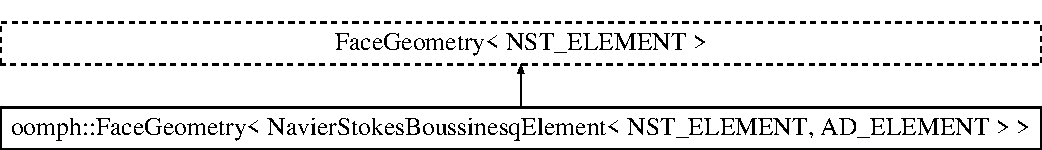
\includegraphics[height=2.000000cm]{classoomph_1_1FaceGeometry_3_01NavierStokesBoussinesqElement_3_01NST__ELEMENT_00_01AD__ELEMENT_01_4_01_4}
\end{center}
\end{figure}
\subsection*{Public Member Functions}
\begin{DoxyCompactItemize}
\item 
\hyperlink{classoomph_1_1FaceGeometry_3_01NavierStokesBoussinesqElement_3_01NST__ELEMENT_00_01AD__ELEMENT_01_4_01_4_ae0a1b0af8c4a6d31491fcc01dc6041a9}{Face\+Geometry} ()
\begin{DoxyCompactList}\small\item\em Constructor calls the constructor of the N\+S\+T\+\_\+\+E\+L\+E\+M\+E\+NT (Only the Intel compiler seems to need this!) \end{DoxyCompactList}\end{DoxyCompactItemize}


\subsection{Detailed Description}
\subsubsection*{template$<$class N\+S\+T\+\_\+\+E\+L\+E\+M\+E\+NT, class A\+D\+\_\+\+E\+L\+E\+M\+E\+NT$>$\newline
class oomph\+::\+Face\+Geometry$<$ Navier\+Stokes\+Boussinesq\+Element$<$ N\+S\+T\+\_\+\+E\+L\+E\+M\+E\+N\+T, A\+D\+\_\+\+E\+L\+E\+M\+E\+N\+T $>$ $>$}

Explicit definition of the face geometry of these elements. 

Definition at line 1017 of file multi\+\_\+domain\+\_\+boussinesq\+\_\+elements.\+h.



\subsection{Constructor \& Destructor Documentation}
\mbox{\Hypertarget{classoomph_1_1FaceGeometry_3_01NavierStokesBoussinesqElement_3_01NST__ELEMENT_00_01AD__ELEMENT_01_4_01_4_ae0a1b0af8c4a6d31491fcc01dc6041a9}\label{classoomph_1_1FaceGeometry_3_01NavierStokesBoussinesqElement_3_01NST__ELEMENT_00_01AD__ELEMENT_01_4_01_4_ae0a1b0af8c4a6d31491fcc01dc6041a9}} 
\index{oomph\+::\+Face\+Geometry$<$ Navier\+Stokes\+Boussinesq\+Element$<$ N\+S\+T\+\_\+\+E\+L\+E\+M\+E\+N\+T, A\+D\+\_\+\+E\+L\+E\+M\+E\+N\+T $>$ $>$@{oomph\+::\+Face\+Geometry$<$ Navier\+Stokes\+Boussinesq\+Element$<$ N\+S\+T\+\_\+\+E\+L\+E\+M\+E\+N\+T, A\+D\+\_\+\+E\+L\+E\+M\+E\+N\+T $>$ $>$}!Face\+Geometry@{Face\+Geometry}}
\index{Face\+Geometry@{Face\+Geometry}!oomph\+::\+Face\+Geometry$<$ Navier\+Stokes\+Boussinesq\+Element$<$ N\+S\+T\+\_\+\+E\+L\+E\+M\+E\+N\+T, A\+D\+\_\+\+E\+L\+E\+M\+E\+N\+T $>$ $>$@{oomph\+::\+Face\+Geometry$<$ Navier\+Stokes\+Boussinesq\+Element$<$ N\+S\+T\+\_\+\+E\+L\+E\+M\+E\+N\+T, A\+D\+\_\+\+E\+L\+E\+M\+E\+N\+T $>$ $>$}}
\subsubsection{\texorpdfstring{Face\+Geometry()}{FaceGeometry()}}
{\footnotesize\ttfamily template$<$class N\+S\+T\+\_\+\+E\+L\+E\+M\+E\+NT , class A\+D\+\_\+\+E\+L\+E\+M\+E\+NT $>$ \\
oomph\+::\+Face\+Geometry$<$ \hyperlink{classoomph_1_1NavierStokesBoussinesqElement}{Navier\+Stokes\+Boussinesq\+Element}$<$ N\+S\+T\+\_\+\+E\+L\+E\+M\+E\+NT, A\+D\+\_\+\+E\+L\+E\+M\+E\+NT $>$ $>$\+::Face\+Geometry (\begin{DoxyParamCaption}{ }\end{DoxyParamCaption})\hspace{0.3cm}{\ttfamily [inline]}}



Constructor calls the constructor of the N\+S\+T\+\_\+\+E\+L\+E\+M\+E\+NT (Only the Intel compiler seems to need this!) 



Definition at line 1023 of file multi\+\_\+domain\+\_\+boussinesq\+\_\+elements.\+h.



The documentation for this class was generated from the following file\+:\begin{DoxyCompactItemize}
\item 
\hyperlink{multi__domain__boussinesq__elements_8h}{multi\+\_\+domain\+\_\+boussinesq\+\_\+elements.\+h}\end{DoxyCompactItemize}

\hypertarget{classoomph_1_1FourierDecomposedHelmholtzFluxFromNormalDisplacementBCElement}{}\section{oomph\+:\+:Fourier\+Decomposed\+Helmholtz\+Flux\+From\+Normal\+Displacement\+B\+C\+Element$<$ H\+E\+L\+M\+H\+O\+L\+T\+Z\+\_\+\+B\+U\+L\+K\+\_\+\+E\+L\+E\+M\+E\+NT, E\+L\+A\+S\+T\+I\+C\+I\+T\+Y\+\_\+\+B\+U\+L\+K\+\_\+\+E\+L\+E\+M\+E\+NT $>$ Class Template Reference}
\label{classoomph_1_1FourierDecomposedHelmholtzFluxFromNormalDisplacementBCElement}\index{oomph\+::\+Fourier\+Decomposed\+Helmholtz\+Flux\+From\+Normal\+Displacement\+B\+C\+Element$<$ H\+E\+L\+M\+H\+O\+L\+T\+Z\+\_\+\+B\+U\+L\+K\+\_\+\+E\+L\+E\+M\+E\+N\+T, E\+L\+A\+S\+T\+I\+C\+I\+T\+Y\+\_\+\+B\+U\+L\+K\+\_\+\+E\+L\+E\+M\+E\+N\+T $>$@{oomph\+::\+Fourier\+Decomposed\+Helmholtz\+Flux\+From\+Normal\+Displacement\+B\+C\+Element$<$ H\+E\+L\+M\+H\+O\+L\+T\+Z\+\_\+\+B\+U\+L\+K\+\_\+\+E\+L\+E\+M\+E\+N\+T, E\+L\+A\+S\+T\+I\+C\+I\+T\+Y\+\_\+\+B\+U\+L\+K\+\_\+\+E\+L\+E\+M\+E\+N\+T $>$}}


A class for elements that allow the imposition of an prescribed flux (determined from the normal displacements of an adjacent linearly elastic solid. Normal derivative for displacement potential is given by normal displacement of adjacent solid multiplies by F\+SI parameter (q = k$^\wedge$2 B/E). The element geometry is obtained from the Face\+Geometry$<$\+E\+L\+E\+M\+E\+N\+T$>$ policy class.  




{\ttfamily \#include $<$fourier\+\_\+decomposed\+\_\+helmholtz\+\_\+time\+\_\+harmonic\+\_\+linear\+\_\+elasticity\+\_\+interaction.\+h$>$}

Inheritance diagram for oomph\+:\+:Fourier\+Decomposed\+Helmholtz\+Flux\+From\+Normal\+Displacement\+B\+C\+Element$<$ H\+E\+L\+M\+H\+O\+L\+T\+Z\+\_\+\+B\+U\+L\+K\+\_\+\+E\+L\+E\+M\+E\+NT, E\+L\+A\+S\+T\+I\+C\+I\+T\+Y\+\_\+\+B\+U\+L\+K\+\_\+\+E\+L\+E\+M\+E\+NT $>$\+:\begin{figure}[H]
\begin{center}
\leavevmode
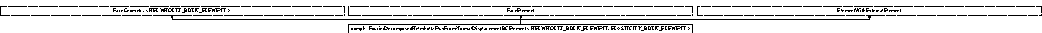
\includegraphics[height=0.440771cm]{classoomph_1_1FourierDecomposedHelmholtzFluxFromNormalDisplacementBCElement}
\end{center}
\end{figure}
\subsection*{Public Member Functions}
\begin{DoxyCompactItemize}
\item 
\hyperlink{classoomph_1_1FourierDecomposedHelmholtzFluxFromNormalDisplacementBCElement_a01e66914352ffdf578cc6ebcfa760dd4}{Fourier\+Decomposed\+Helmholtz\+Flux\+From\+Normal\+Displacement\+B\+C\+Element} (Finite\+Element $\ast$const \&bulk\+\_\+el\+\_\+pt, const int \&face\+\_\+index)
\begin{DoxyCompactList}\small\item\em Constructor, takes the pointer to the \char`\"{}bulk\char`\"{} element and the face index identifying the face to which the element is attached. \end{DoxyCompactList}\item 
\hyperlink{classoomph_1_1FourierDecomposedHelmholtzFluxFromNormalDisplacementBCElement_aafab69b927f48ec192cf48cf7fde7712}{Fourier\+Decomposed\+Helmholtz\+Flux\+From\+Normal\+Displacement\+B\+C\+Element} (const \hyperlink{classoomph_1_1FourierDecomposedHelmholtzFluxFromNormalDisplacementBCElement}{Fourier\+Decomposed\+Helmholtz\+Flux\+From\+Normal\+Displacement\+B\+C\+Element} \&dummy)
\begin{DoxyCompactList}\small\item\em Broken copy constructor. \end{DoxyCompactList}\item 
void \hyperlink{classoomph_1_1FourierDecomposedHelmholtzFluxFromNormalDisplacementBCElement_a9fb0fe9492372a7687b6e30b00d257c1}{fill\+\_\+in\+\_\+contribution\+\_\+to\+\_\+residuals} (Vector$<$ double $>$ \&residuals)
\begin{DoxyCompactList}\small\item\em Broken assignment operator. \end{DoxyCompactList}\item 
void \hyperlink{classoomph_1_1FourierDecomposedHelmholtzFluxFromNormalDisplacementBCElement_a721d81ba5e0e9c8d811303e7a9ce5a8a}{fill\+\_\+in\+\_\+contribution\+\_\+to\+\_\+jacobian} (Vector$<$ double $>$ \&residuals, Dense\+Matrix$<$ double $>$ \&jacobian)
\begin{DoxyCompactList}\small\item\em Add the element\textquotesingle{}s contribution to its residual vector and its Jacobian matrix. \end{DoxyCompactList}\item 
void \hyperlink{classoomph_1_1FourierDecomposedHelmholtzFluxFromNormalDisplacementBCElement_a3846857ca5fe15cc5c8020d8f0117b67}{output} (std\+::ostream \&outfile)
\begin{DoxyCompactList}\small\item\em Output function. \end{DoxyCompactList}\item 
void \hyperlink{classoomph_1_1FourierDecomposedHelmholtzFluxFromNormalDisplacementBCElement_ac69b78e1f4cf73d3dbe07d8e1dbfe0b1}{output} (std\+::ostream \&outfile, const unsigned \&n\+\_\+plot)
\begin{DoxyCompactList}\small\item\em Output function\+: flux etc at Gauss points; n\+\_\+plot is ignored. \end{DoxyCompactList}\item 
void \hyperlink{classoomph_1_1FourierDecomposedHelmholtzFluxFromNormalDisplacementBCElement_aab3531a5a9c6a1a1fb4d2e9051e22c7e}{output} (F\+I\+LE $\ast$file\+\_\+pt)
\begin{DoxyCompactList}\small\item\em C-\/style output function. \end{DoxyCompactList}\item 
void \hyperlink{classoomph_1_1FourierDecomposedHelmholtzFluxFromNormalDisplacementBCElement_a982a948fa62759e5cb2e7953bb891602}{output} (F\+I\+LE $\ast$file\+\_\+pt, const unsigned \&n\+\_\+plot)
\begin{DoxyCompactList}\small\item\em C-\/style output function. \end{DoxyCompactList}\end{DoxyCompactItemize}
\subsection*{Protected Member Functions}
\begin{DoxyCompactItemize}
\item 
double \hyperlink{classoomph_1_1FourierDecomposedHelmholtzFluxFromNormalDisplacementBCElement_ae9aa741774cfc14e95ff9113844119f5}{shape\+\_\+and\+\_\+test} (const Vector$<$ double $>$ \&s, Shape \&psi, Shape \&test) const
\begin{DoxyCompactList}\small\item\em Function to compute the shape and test functions and to return the Jacobian of mapping between local and global (Eulerian) coordinates. \end{DoxyCompactList}\item 
double \hyperlink{classoomph_1_1FourierDecomposedHelmholtzFluxFromNormalDisplacementBCElement_ab9f53637a61bc8a089170011596e5184}{shape\+\_\+and\+\_\+test\+\_\+at\+\_\+knot} (const unsigned \&ipt, Shape \&psi, Shape \&test) const
\begin{DoxyCompactList}\small\item\em Function to compute the shape and test functions and to return. \end{DoxyCompactList}\end{DoxyCompactItemize}
\subsection*{Private Member Functions}
\begin{DoxyCompactItemize}
\item 
void \hyperlink{classoomph_1_1FourierDecomposedHelmholtzFluxFromNormalDisplacementBCElement_a15c86be276d382c3b948f5f8115d3261}{fill\+\_\+in\+\_\+generic\+\_\+residual\+\_\+contribution\+\_\+helmholtz\+\_\+flux\+\_\+from\+\_\+displacement} (Vector$<$ double $>$ \&residuals, Dense\+Matrix$<$ double $>$ \&jacobian, const unsigned \&flag)
\begin{DoxyCompactList}\small\item\em Add the element\textquotesingle{}s contribution to its residual vector. flag=1(or 0)\+: do (or don\textquotesingle{}t) compute the contribution to the Jacobian as well. \end{DoxyCompactList}\end{DoxyCompactItemize}
\subsection*{Private Attributes}
\begin{DoxyCompactItemize}
\item 
unsigned \hyperlink{classoomph_1_1FourierDecomposedHelmholtzFluxFromNormalDisplacementBCElement_ac3f8d4afa7b803c75d7f3cb8e07a48ca}{Dim}
\begin{DoxyCompactList}\small\item\em The spatial dimension of the problem. \end{DoxyCompactList}\item 
std\+::complex$<$ unsigned $>$ \hyperlink{classoomph_1_1FourierDecomposedHelmholtzFluxFromNormalDisplacementBCElement_a5b1225f509b692ab0027477785a56d35}{U\+\_\+index\+\_\+helmholtz\+\_\+from\+\_\+displacement}
\begin{DoxyCompactList}\small\item\em The index at which the unknown is stored at the nodes. \end{DoxyCompactList}\end{DoxyCompactItemize}


\subsection{Detailed Description}
\subsubsection*{template$<$class H\+E\+L\+M\+H\+O\+L\+T\+Z\+\_\+\+B\+U\+L\+K\+\_\+\+E\+L\+E\+M\+E\+NT, class E\+L\+A\+S\+T\+I\+C\+I\+T\+Y\+\_\+\+B\+U\+L\+K\+\_\+\+E\+L\+E\+M\+E\+NT$>$\newline
class oomph\+::\+Fourier\+Decomposed\+Helmholtz\+Flux\+From\+Normal\+Displacement\+B\+C\+Element$<$ H\+E\+L\+M\+H\+O\+L\+T\+Z\+\_\+\+B\+U\+L\+K\+\_\+\+E\+L\+E\+M\+E\+N\+T, E\+L\+A\+S\+T\+I\+C\+I\+T\+Y\+\_\+\+B\+U\+L\+K\+\_\+\+E\+L\+E\+M\+E\+N\+T $>$}

A class for elements that allow the imposition of an prescribed flux (determined from the normal displacements of an adjacent linearly elastic solid. Normal derivative for displacement potential is given by normal displacement of adjacent solid multiplies by F\+SI parameter (q = k$^\wedge$2 B/E). The element geometry is obtained from the Face\+Geometry$<$\+E\+L\+E\+M\+E\+N\+T$>$ policy class. 

Definition at line 452 of file fourier\+\_\+decomposed\+\_\+helmholtz\+\_\+time\+\_\+harmonic\+\_\+linear\+\_\+elasticity\+\_\+interaction.\+h.



\subsection{Constructor \& Destructor Documentation}
\mbox{\Hypertarget{classoomph_1_1FourierDecomposedHelmholtzFluxFromNormalDisplacementBCElement_a01e66914352ffdf578cc6ebcfa760dd4}\label{classoomph_1_1FourierDecomposedHelmholtzFluxFromNormalDisplacementBCElement_a01e66914352ffdf578cc6ebcfa760dd4}} 
\index{oomph\+::\+Fourier\+Decomposed\+Helmholtz\+Flux\+From\+Normal\+Displacement\+B\+C\+Element@{oomph\+::\+Fourier\+Decomposed\+Helmholtz\+Flux\+From\+Normal\+Displacement\+B\+C\+Element}!Fourier\+Decomposed\+Helmholtz\+Flux\+From\+Normal\+Displacement\+B\+C\+Element@{Fourier\+Decomposed\+Helmholtz\+Flux\+From\+Normal\+Displacement\+B\+C\+Element}}
\index{Fourier\+Decomposed\+Helmholtz\+Flux\+From\+Normal\+Displacement\+B\+C\+Element@{Fourier\+Decomposed\+Helmholtz\+Flux\+From\+Normal\+Displacement\+B\+C\+Element}!oomph\+::\+Fourier\+Decomposed\+Helmholtz\+Flux\+From\+Normal\+Displacement\+B\+C\+Element@{oomph\+::\+Fourier\+Decomposed\+Helmholtz\+Flux\+From\+Normal\+Displacement\+B\+C\+Element}}
\subsubsection{\texorpdfstring{Fourier\+Decomposed\+Helmholtz\+Flux\+From\+Normal\+Displacement\+B\+C\+Element()}{FourierDecomposedHelmholtzFluxFromNormalDisplacementBCElement()}\hspace{0.1cm}{\footnotesize\ttfamily [1/2]}}
{\footnotesize\ttfamily template$<$class H\+E\+L\+M\+H\+O\+L\+T\+Z\+\_\+\+B\+U\+L\+K\+\_\+\+E\+L\+E\+M\+E\+NT , class E\+L\+A\+S\+T\+I\+C\+I\+T\+Y\+\_\+\+B\+U\+L\+K\+\_\+\+E\+L\+E\+M\+E\+NT $>$ \\
\hyperlink{classoomph_1_1FourierDecomposedHelmholtzFluxFromNormalDisplacementBCElement}{oomph\+::\+Fourier\+Decomposed\+Helmholtz\+Flux\+From\+Normal\+Displacement\+B\+C\+Element}$<$ H\+E\+L\+M\+H\+O\+L\+T\+Z\+\_\+\+B\+U\+L\+K\+\_\+\+E\+L\+E\+M\+E\+NT, E\+L\+A\+S\+T\+I\+C\+I\+T\+Y\+\_\+\+B\+U\+L\+K\+\_\+\+E\+L\+E\+M\+E\+NT $>$\+::\hyperlink{classoomph_1_1FourierDecomposedHelmholtzFluxFromNormalDisplacementBCElement}{Fourier\+Decomposed\+Helmholtz\+Flux\+From\+Normal\+Displacement\+B\+C\+Element} (\begin{DoxyParamCaption}\item[{Finite\+Element $\ast$const \&}]{bulk\+\_\+el\+\_\+pt,  }\item[{const int \&}]{face\+\_\+index }\end{DoxyParamCaption})}



Constructor, takes the pointer to the \char`\"{}bulk\char`\"{} element and the face index identifying the face to which the element is attached. 

Constructor, takes the pointer to the \char`\"{}bulk\char`\"{} element, and the face index that identifies the face of the bulk element to which this face element is to be attached. 

Definition at line 659 of file fourier\+\_\+decomposed\+\_\+helmholtz\+\_\+time\+\_\+harmonic\+\_\+linear\+\_\+elasticity\+\_\+interaction.\+h.



References oomph\+::\+Fourier\+Decomposed\+Helmholtz\+Flux\+From\+Normal\+Displacement\+B\+C\+Element$<$ H\+E\+L\+M\+H\+O\+L\+T\+Z\+\_\+\+B\+U\+L\+K\+\_\+\+E\+L\+E\+M\+E\+N\+T, E\+L\+A\+S\+T\+I\+C\+I\+T\+Y\+\_\+\+B\+U\+L\+K\+\_\+\+E\+L\+E\+M\+E\+N\+T $>$\+::\+Dim, oomph\+::\+Fourier\+Decomposed\+Helmholtz\+Flux\+From\+Normal\+Displacement\+B\+C\+Element$<$ H\+E\+L\+M\+H\+O\+L\+T\+Z\+\_\+\+B\+U\+L\+K\+\_\+\+E\+L\+E\+M\+E\+N\+T, E\+L\+A\+S\+T\+I\+C\+I\+T\+Y\+\_\+\+B\+U\+L\+K\+\_\+\+E\+L\+E\+M\+E\+N\+T $>$\+::fill\+\_\+in\+\_\+generic\+\_\+residual\+\_\+contribution\+\_\+helmholtz\+\_\+flux\+\_\+from\+\_\+displacement(), and oomph\+::\+Fourier\+Decomposed\+Helmholtz\+Flux\+From\+Normal\+Displacement\+B\+C\+Element$<$ H\+E\+L\+M\+H\+O\+L\+T\+Z\+\_\+\+B\+U\+L\+K\+\_\+\+E\+L\+E\+M\+E\+N\+T, E\+L\+A\+S\+T\+I\+C\+I\+T\+Y\+\_\+\+B\+U\+L\+K\+\_\+\+E\+L\+E\+M\+E\+N\+T $>$\+::\+U\+\_\+index\+\_\+helmholtz\+\_\+from\+\_\+displacement.

\mbox{\Hypertarget{classoomph_1_1FourierDecomposedHelmholtzFluxFromNormalDisplacementBCElement_aafab69b927f48ec192cf48cf7fde7712}\label{classoomph_1_1FourierDecomposedHelmholtzFluxFromNormalDisplacementBCElement_aafab69b927f48ec192cf48cf7fde7712}} 
\index{oomph\+::\+Fourier\+Decomposed\+Helmholtz\+Flux\+From\+Normal\+Displacement\+B\+C\+Element@{oomph\+::\+Fourier\+Decomposed\+Helmholtz\+Flux\+From\+Normal\+Displacement\+B\+C\+Element}!Fourier\+Decomposed\+Helmholtz\+Flux\+From\+Normal\+Displacement\+B\+C\+Element@{Fourier\+Decomposed\+Helmholtz\+Flux\+From\+Normal\+Displacement\+B\+C\+Element}}
\index{Fourier\+Decomposed\+Helmholtz\+Flux\+From\+Normal\+Displacement\+B\+C\+Element@{Fourier\+Decomposed\+Helmholtz\+Flux\+From\+Normal\+Displacement\+B\+C\+Element}!oomph\+::\+Fourier\+Decomposed\+Helmholtz\+Flux\+From\+Normal\+Displacement\+B\+C\+Element@{oomph\+::\+Fourier\+Decomposed\+Helmholtz\+Flux\+From\+Normal\+Displacement\+B\+C\+Element}}
\subsubsection{\texorpdfstring{Fourier\+Decomposed\+Helmholtz\+Flux\+From\+Normal\+Displacement\+B\+C\+Element()}{FourierDecomposedHelmholtzFluxFromNormalDisplacementBCElement()}\hspace{0.1cm}{\footnotesize\ttfamily [2/2]}}
{\footnotesize\ttfamily template$<$class H\+E\+L\+M\+H\+O\+L\+T\+Z\+\_\+\+B\+U\+L\+K\+\_\+\+E\+L\+E\+M\+E\+NT , class E\+L\+A\+S\+T\+I\+C\+I\+T\+Y\+\_\+\+B\+U\+L\+K\+\_\+\+E\+L\+E\+M\+E\+NT $>$ \\
\hyperlink{classoomph_1_1FourierDecomposedHelmholtzFluxFromNormalDisplacementBCElement}{oomph\+::\+Fourier\+Decomposed\+Helmholtz\+Flux\+From\+Normal\+Displacement\+B\+C\+Element}$<$ H\+E\+L\+M\+H\+O\+L\+T\+Z\+\_\+\+B\+U\+L\+K\+\_\+\+E\+L\+E\+M\+E\+NT, E\+L\+A\+S\+T\+I\+C\+I\+T\+Y\+\_\+\+B\+U\+L\+K\+\_\+\+E\+L\+E\+M\+E\+NT $>$\+::\hyperlink{classoomph_1_1FourierDecomposedHelmholtzFluxFromNormalDisplacementBCElement}{Fourier\+Decomposed\+Helmholtz\+Flux\+From\+Normal\+Displacement\+B\+C\+Element} (\begin{DoxyParamCaption}\item[{const \hyperlink{classoomph_1_1FourierDecomposedHelmholtzFluxFromNormalDisplacementBCElement}{Fourier\+Decomposed\+Helmholtz\+Flux\+From\+Normal\+Displacement\+B\+C\+Element}$<$ H\+E\+L\+M\+H\+O\+L\+T\+Z\+\_\+\+B\+U\+L\+K\+\_\+\+E\+L\+E\+M\+E\+NT, E\+L\+A\+S\+T\+I\+C\+I\+T\+Y\+\_\+\+B\+U\+L\+K\+\_\+\+E\+L\+E\+M\+E\+NT $>$ \&}]{dummy }\end{DoxyParamCaption})\hspace{0.3cm}{\ttfamily [inline]}}



Broken copy constructor. 



Definition at line 468 of file fourier\+\_\+decomposed\+\_\+helmholtz\+\_\+time\+\_\+harmonic\+\_\+linear\+\_\+elasticity\+\_\+interaction.\+h.



\subsection{Member Function Documentation}
\mbox{\Hypertarget{classoomph_1_1FourierDecomposedHelmholtzFluxFromNormalDisplacementBCElement_a721d81ba5e0e9c8d811303e7a9ce5a8a}\label{classoomph_1_1FourierDecomposedHelmholtzFluxFromNormalDisplacementBCElement_a721d81ba5e0e9c8d811303e7a9ce5a8a}} 
\index{oomph\+::\+Fourier\+Decomposed\+Helmholtz\+Flux\+From\+Normal\+Displacement\+B\+C\+Element@{oomph\+::\+Fourier\+Decomposed\+Helmholtz\+Flux\+From\+Normal\+Displacement\+B\+C\+Element}!fill\+\_\+in\+\_\+contribution\+\_\+to\+\_\+jacobian@{fill\+\_\+in\+\_\+contribution\+\_\+to\+\_\+jacobian}}
\index{fill\+\_\+in\+\_\+contribution\+\_\+to\+\_\+jacobian@{fill\+\_\+in\+\_\+contribution\+\_\+to\+\_\+jacobian}!oomph\+::\+Fourier\+Decomposed\+Helmholtz\+Flux\+From\+Normal\+Displacement\+B\+C\+Element@{oomph\+::\+Fourier\+Decomposed\+Helmholtz\+Flux\+From\+Normal\+Displacement\+B\+C\+Element}}
\subsubsection{\texorpdfstring{fill\+\_\+in\+\_\+contribution\+\_\+to\+\_\+jacobian()}{fill\_in\_contribution\_to\_jacobian()}}
{\footnotesize\ttfamily template$<$class H\+E\+L\+M\+H\+O\+L\+T\+Z\+\_\+\+B\+U\+L\+K\+\_\+\+E\+L\+E\+M\+E\+NT , class E\+L\+A\+S\+T\+I\+C\+I\+T\+Y\+\_\+\+B\+U\+L\+K\+\_\+\+E\+L\+E\+M\+E\+NT $>$ \\
void \hyperlink{classoomph_1_1FourierDecomposedHelmholtzFluxFromNormalDisplacementBCElement}{oomph\+::\+Fourier\+Decomposed\+Helmholtz\+Flux\+From\+Normal\+Displacement\+B\+C\+Element}$<$ H\+E\+L\+M\+H\+O\+L\+T\+Z\+\_\+\+B\+U\+L\+K\+\_\+\+E\+L\+E\+M\+E\+NT, E\+L\+A\+S\+T\+I\+C\+I\+T\+Y\+\_\+\+B\+U\+L\+K\+\_\+\+E\+L\+E\+M\+E\+NT $>$\+::fill\+\_\+in\+\_\+contribution\+\_\+to\+\_\+jacobian (\begin{DoxyParamCaption}\item[{Vector$<$ double $>$ \&}]{residuals,  }\item[{Dense\+Matrix$<$ double $>$ \&}]{jacobian }\end{DoxyParamCaption})\hspace{0.3cm}{\ttfamily [inline]}}



Add the element\textquotesingle{}s contribution to its residual vector and its Jacobian matrix. 



Definition at line 500 of file fourier\+\_\+decomposed\+\_\+helmholtz\+\_\+time\+\_\+harmonic\+\_\+linear\+\_\+elasticity\+\_\+interaction.\+h.

\mbox{\Hypertarget{classoomph_1_1FourierDecomposedHelmholtzFluxFromNormalDisplacementBCElement_a9fb0fe9492372a7687b6e30b00d257c1}\label{classoomph_1_1FourierDecomposedHelmholtzFluxFromNormalDisplacementBCElement_a9fb0fe9492372a7687b6e30b00d257c1}} 
\index{oomph\+::\+Fourier\+Decomposed\+Helmholtz\+Flux\+From\+Normal\+Displacement\+B\+C\+Element@{oomph\+::\+Fourier\+Decomposed\+Helmholtz\+Flux\+From\+Normal\+Displacement\+B\+C\+Element}!fill\+\_\+in\+\_\+contribution\+\_\+to\+\_\+residuals@{fill\+\_\+in\+\_\+contribution\+\_\+to\+\_\+residuals}}
\index{fill\+\_\+in\+\_\+contribution\+\_\+to\+\_\+residuals@{fill\+\_\+in\+\_\+contribution\+\_\+to\+\_\+residuals}!oomph\+::\+Fourier\+Decomposed\+Helmholtz\+Flux\+From\+Normal\+Displacement\+B\+C\+Element@{oomph\+::\+Fourier\+Decomposed\+Helmholtz\+Flux\+From\+Normal\+Displacement\+B\+C\+Element}}
\subsubsection{\texorpdfstring{fill\+\_\+in\+\_\+contribution\+\_\+to\+\_\+residuals()}{fill\_in\_contribution\_to\_residuals()}}
{\footnotesize\ttfamily template$<$class H\+E\+L\+M\+H\+O\+L\+T\+Z\+\_\+\+B\+U\+L\+K\+\_\+\+E\+L\+E\+M\+E\+NT , class E\+L\+A\+S\+T\+I\+C\+I\+T\+Y\+\_\+\+B\+U\+L\+K\+\_\+\+E\+L\+E\+M\+E\+NT $>$ \\
void \hyperlink{classoomph_1_1FourierDecomposedHelmholtzFluxFromNormalDisplacementBCElement}{oomph\+::\+Fourier\+Decomposed\+Helmholtz\+Flux\+From\+Normal\+Displacement\+B\+C\+Element}$<$ H\+E\+L\+M\+H\+O\+L\+T\+Z\+\_\+\+B\+U\+L\+K\+\_\+\+E\+L\+E\+M\+E\+NT, E\+L\+A\+S\+T\+I\+C\+I\+T\+Y\+\_\+\+B\+U\+L\+K\+\_\+\+E\+L\+E\+M\+E\+NT $>$\+::fill\+\_\+in\+\_\+contribution\+\_\+to\+\_\+residuals (\begin{DoxyParamCaption}\item[{Vector$<$ double $>$ \&}]{residuals }\end{DoxyParamCaption})\hspace{0.3cm}{\ttfamily [inline]}}



Broken assignment operator. 

Add the element\textquotesingle{}s contribution to its residual vector 

Definition at line 489 of file fourier\+\_\+decomposed\+\_\+helmholtz\+\_\+time\+\_\+harmonic\+\_\+linear\+\_\+elasticity\+\_\+interaction.\+h.

\mbox{\Hypertarget{classoomph_1_1FourierDecomposedHelmholtzFluxFromNormalDisplacementBCElement_a15c86be276d382c3b948f5f8115d3261}\label{classoomph_1_1FourierDecomposedHelmholtzFluxFromNormalDisplacementBCElement_a15c86be276d382c3b948f5f8115d3261}} 
\index{oomph\+::\+Fourier\+Decomposed\+Helmholtz\+Flux\+From\+Normal\+Displacement\+B\+C\+Element@{oomph\+::\+Fourier\+Decomposed\+Helmholtz\+Flux\+From\+Normal\+Displacement\+B\+C\+Element}!fill\+\_\+in\+\_\+generic\+\_\+residual\+\_\+contribution\+\_\+helmholtz\+\_\+flux\+\_\+from\+\_\+displacement@{fill\+\_\+in\+\_\+generic\+\_\+residual\+\_\+contribution\+\_\+helmholtz\+\_\+flux\+\_\+from\+\_\+displacement}}
\index{fill\+\_\+in\+\_\+generic\+\_\+residual\+\_\+contribution\+\_\+helmholtz\+\_\+flux\+\_\+from\+\_\+displacement@{fill\+\_\+in\+\_\+generic\+\_\+residual\+\_\+contribution\+\_\+helmholtz\+\_\+flux\+\_\+from\+\_\+displacement}!oomph\+::\+Fourier\+Decomposed\+Helmholtz\+Flux\+From\+Normal\+Displacement\+B\+C\+Element@{oomph\+::\+Fourier\+Decomposed\+Helmholtz\+Flux\+From\+Normal\+Displacement\+B\+C\+Element}}
\subsubsection{\texorpdfstring{fill\+\_\+in\+\_\+generic\+\_\+residual\+\_\+contribution\+\_\+helmholtz\+\_\+flux\+\_\+from\+\_\+displacement()}{fill\_in\_generic\_residual\_contribution\_helmholtz\_flux\_from\_displacement()}}
{\footnotesize\ttfamily template$<$class H\+E\+L\+M\+H\+O\+L\+T\+Z\+\_\+\+B\+U\+L\+K\+\_\+\+E\+L\+E\+M\+E\+NT , class E\+L\+A\+S\+T\+I\+C\+I\+T\+Y\+\_\+\+B\+U\+L\+K\+\_\+\+E\+L\+E\+M\+E\+NT $>$ \\
void \hyperlink{classoomph_1_1FourierDecomposedHelmholtzFluxFromNormalDisplacementBCElement}{oomph\+::\+Fourier\+Decomposed\+Helmholtz\+Flux\+From\+Normal\+Displacement\+B\+C\+Element}$<$ H\+E\+L\+M\+H\+O\+L\+T\+Z\+\_\+\+B\+U\+L\+K\+\_\+\+E\+L\+E\+M\+E\+NT, E\+L\+A\+S\+T\+I\+C\+I\+T\+Y\+\_\+\+B\+U\+L\+K\+\_\+\+E\+L\+E\+M\+E\+NT $>$\+::fill\+\_\+in\+\_\+generic\+\_\+residual\+\_\+contribution\+\_\+helmholtz\+\_\+flux\+\_\+from\+\_\+displacement (\begin{DoxyParamCaption}\item[{Vector$<$ double $>$ \&}]{residuals,  }\item[{Dense\+Matrix$<$ double $>$ \&}]{jacobian,  }\item[{const unsigned \&}]{flag }\end{DoxyParamCaption})\hspace{0.3cm}{\ttfamily [private]}}



Add the element\textquotesingle{}s contribution to its residual vector. flag=1(or 0)\+: do (or don\textquotesingle{}t) compute the contribution to the Jacobian as well. 

Helper function to compute the element\textquotesingle{}s residual vector and the Jacobian matrix. 

Definition at line 751 of file fourier\+\_\+decomposed\+\_\+helmholtz\+\_\+time\+\_\+harmonic\+\_\+linear\+\_\+elasticity\+\_\+interaction.\+h.



References oomph\+::\+Fourier\+Decomposed\+Helmholtz\+Flux\+From\+Normal\+Displacement\+B\+C\+Element$<$ H\+E\+L\+M\+H\+O\+L\+T\+Z\+\_\+\+B\+U\+L\+K\+\_\+\+E\+L\+E\+M\+E\+N\+T, E\+L\+A\+S\+T\+I\+C\+I\+T\+Y\+\_\+\+B\+U\+L\+K\+\_\+\+E\+L\+E\+M\+E\+N\+T $>$\+::\+Dim, oomph\+::\+Fourier\+Decomposed\+Helmholtz\+Flux\+From\+Normal\+Displacement\+B\+C\+Element$<$ H\+E\+L\+M\+H\+O\+L\+T\+Z\+\_\+\+B\+U\+L\+K\+\_\+\+E\+L\+E\+M\+E\+N\+T, E\+L\+A\+S\+T\+I\+C\+I\+T\+Y\+\_\+\+B\+U\+L\+K\+\_\+\+E\+L\+E\+M\+E\+N\+T $>$\+::shape\+\_\+and\+\_\+test(), and oomph\+::\+Fourier\+Decomposed\+Helmholtz\+Flux\+From\+Normal\+Displacement\+B\+C\+Element$<$ H\+E\+L\+M\+H\+O\+L\+T\+Z\+\_\+\+B\+U\+L\+K\+\_\+\+E\+L\+E\+M\+E\+N\+T, E\+L\+A\+S\+T\+I\+C\+I\+T\+Y\+\_\+\+B\+U\+L\+K\+\_\+\+E\+L\+E\+M\+E\+N\+T $>$\+::\+U\+\_\+index\+\_\+helmholtz\+\_\+from\+\_\+displacement.



Referenced by oomph\+::\+Fourier\+Decomposed\+Helmholtz\+Flux\+From\+Normal\+Displacement\+B\+C\+Element$<$ H\+E\+L\+M\+H\+O\+L\+T\+Z\+\_\+\+B\+U\+L\+K\+\_\+\+E\+L\+E\+M\+E\+N\+T, E\+L\+A\+S\+T\+I\+C\+I\+T\+Y\+\_\+\+B\+U\+L\+K\+\_\+\+E\+L\+E\+M\+E\+N\+T $>$\+::\+Fourier\+Decomposed\+Helmholtz\+Flux\+From\+Normal\+Displacement\+B\+C\+Element().

\mbox{\Hypertarget{classoomph_1_1FourierDecomposedHelmholtzFluxFromNormalDisplacementBCElement_a3846857ca5fe15cc5c8020d8f0117b67}\label{classoomph_1_1FourierDecomposedHelmholtzFluxFromNormalDisplacementBCElement_a3846857ca5fe15cc5c8020d8f0117b67}} 
\index{oomph\+::\+Fourier\+Decomposed\+Helmholtz\+Flux\+From\+Normal\+Displacement\+B\+C\+Element@{oomph\+::\+Fourier\+Decomposed\+Helmholtz\+Flux\+From\+Normal\+Displacement\+B\+C\+Element}!output@{output}}
\index{output@{output}!oomph\+::\+Fourier\+Decomposed\+Helmholtz\+Flux\+From\+Normal\+Displacement\+B\+C\+Element@{oomph\+::\+Fourier\+Decomposed\+Helmholtz\+Flux\+From\+Normal\+Displacement\+B\+C\+Element}}
\subsubsection{\texorpdfstring{output()}{output()}\hspace{0.1cm}{\footnotesize\ttfamily [1/4]}}
{\footnotesize\ttfamily template$<$class H\+E\+L\+M\+H\+O\+L\+T\+Z\+\_\+\+B\+U\+L\+K\+\_\+\+E\+L\+E\+M\+E\+NT , class E\+L\+A\+S\+T\+I\+C\+I\+T\+Y\+\_\+\+B\+U\+L\+K\+\_\+\+E\+L\+E\+M\+E\+NT $>$ \\
void \hyperlink{classoomph_1_1FourierDecomposedHelmholtzFluxFromNormalDisplacementBCElement}{oomph\+::\+Fourier\+Decomposed\+Helmholtz\+Flux\+From\+Normal\+Displacement\+B\+C\+Element}$<$ H\+E\+L\+M\+H\+O\+L\+T\+Z\+\_\+\+B\+U\+L\+K\+\_\+\+E\+L\+E\+M\+E\+NT, E\+L\+A\+S\+T\+I\+C\+I\+T\+Y\+\_\+\+B\+U\+L\+K\+\_\+\+E\+L\+E\+M\+E\+NT $>$\+::output (\begin{DoxyParamCaption}\item[{std\+::ostream \&}]{outfile }\end{DoxyParamCaption})\hspace{0.3cm}{\ttfamily [inline]}}



Output function. 



Definition at line 512 of file fourier\+\_\+decomposed\+\_\+helmholtz\+\_\+time\+\_\+harmonic\+\_\+linear\+\_\+elasticity\+\_\+interaction.\+h.



References oomph\+::\+Fourier\+Decomposed\+Time\+Harmonic\+Lin\+Elast\+Loaded\+By\+Helmholtz\+Pressure\+B\+C\+Element$<$ E\+L\+A\+S\+T\+I\+C\+I\+T\+Y\+\_\+\+B\+U\+L\+K\+\_\+\+E\+L\+E\+M\+E\+N\+T, H\+E\+L\+M\+H\+O\+L\+T\+Z\+\_\+\+B\+U\+L\+K\+\_\+\+E\+L\+E\+M\+E\+N\+T $>$\+::output().

\mbox{\Hypertarget{classoomph_1_1FourierDecomposedHelmholtzFluxFromNormalDisplacementBCElement_ac69b78e1f4cf73d3dbe07d8e1dbfe0b1}\label{classoomph_1_1FourierDecomposedHelmholtzFluxFromNormalDisplacementBCElement_ac69b78e1f4cf73d3dbe07d8e1dbfe0b1}} 
\index{oomph\+::\+Fourier\+Decomposed\+Helmholtz\+Flux\+From\+Normal\+Displacement\+B\+C\+Element@{oomph\+::\+Fourier\+Decomposed\+Helmholtz\+Flux\+From\+Normal\+Displacement\+B\+C\+Element}!output@{output}}
\index{output@{output}!oomph\+::\+Fourier\+Decomposed\+Helmholtz\+Flux\+From\+Normal\+Displacement\+B\+C\+Element@{oomph\+::\+Fourier\+Decomposed\+Helmholtz\+Flux\+From\+Normal\+Displacement\+B\+C\+Element}}
\subsubsection{\texorpdfstring{output()}{output()}\hspace{0.1cm}{\footnotesize\ttfamily [2/4]}}
{\footnotesize\ttfamily template$<$class H\+E\+L\+M\+H\+O\+L\+T\+Z\+\_\+\+B\+U\+L\+K\+\_\+\+E\+L\+E\+M\+E\+NT , class E\+L\+A\+S\+T\+I\+C\+I\+T\+Y\+\_\+\+B\+U\+L\+K\+\_\+\+E\+L\+E\+M\+E\+NT $>$ \\
void \hyperlink{classoomph_1_1FourierDecomposedHelmholtzFluxFromNormalDisplacementBCElement}{oomph\+::\+Fourier\+Decomposed\+Helmholtz\+Flux\+From\+Normal\+Displacement\+B\+C\+Element}$<$ H\+E\+L\+M\+H\+O\+L\+T\+Z\+\_\+\+B\+U\+L\+K\+\_\+\+E\+L\+E\+M\+E\+NT, E\+L\+A\+S\+T\+I\+C\+I\+T\+Y\+\_\+\+B\+U\+L\+K\+\_\+\+E\+L\+E\+M\+E\+NT $>$\+::output (\begin{DoxyParamCaption}\item[{std\+::ostream \&}]{outfile,  }\item[{const unsigned \&}]{n\+\_\+plot }\end{DoxyParamCaption})\hspace{0.3cm}{\ttfamily [inline]}}



Output function\+: flux etc at Gauss points; n\+\_\+plot is ignored. 



Definition at line 520 of file fourier\+\_\+decomposed\+\_\+helmholtz\+\_\+time\+\_\+harmonic\+\_\+linear\+\_\+elasticity\+\_\+interaction.\+h.

\mbox{\Hypertarget{classoomph_1_1FourierDecomposedHelmholtzFluxFromNormalDisplacementBCElement_aab3531a5a9c6a1a1fb4d2e9051e22c7e}\label{classoomph_1_1FourierDecomposedHelmholtzFluxFromNormalDisplacementBCElement_aab3531a5a9c6a1a1fb4d2e9051e22c7e}} 
\index{oomph\+::\+Fourier\+Decomposed\+Helmholtz\+Flux\+From\+Normal\+Displacement\+B\+C\+Element@{oomph\+::\+Fourier\+Decomposed\+Helmholtz\+Flux\+From\+Normal\+Displacement\+B\+C\+Element}!output@{output}}
\index{output@{output}!oomph\+::\+Fourier\+Decomposed\+Helmholtz\+Flux\+From\+Normal\+Displacement\+B\+C\+Element@{oomph\+::\+Fourier\+Decomposed\+Helmholtz\+Flux\+From\+Normal\+Displacement\+B\+C\+Element}}
\subsubsection{\texorpdfstring{output()}{output()}\hspace{0.1cm}{\footnotesize\ttfamily [3/4]}}
{\footnotesize\ttfamily template$<$class H\+E\+L\+M\+H\+O\+L\+T\+Z\+\_\+\+B\+U\+L\+K\+\_\+\+E\+L\+E\+M\+E\+NT , class E\+L\+A\+S\+T\+I\+C\+I\+T\+Y\+\_\+\+B\+U\+L\+K\+\_\+\+E\+L\+E\+M\+E\+NT $>$ \\
void \hyperlink{classoomph_1_1FourierDecomposedHelmholtzFluxFromNormalDisplacementBCElement}{oomph\+::\+Fourier\+Decomposed\+Helmholtz\+Flux\+From\+Normal\+Displacement\+B\+C\+Element}$<$ H\+E\+L\+M\+H\+O\+L\+T\+Z\+\_\+\+B\+U\+L\+K\+\_\+\+E\+L\+E\+M\+E\+NT, E\+L\+A\+S\+T\+I\+C\+I\+T\+Y\+\_\+\+B\+U\+L\+K\+\_\+\+E\+L\+E\+M\+E\+NT $>$\+::output (\begin{DoxyParamCaption}\item[{F\+I\+LE $\ast$}]{file\+\_\+pt }\end{DoxyParamCaption})\hspace{0.3cm}{\ttfamily [inline]}}



C-\/style output function. 



Definition at line 573 of file fourier\+\_\+decomposed\+\_\+helmholtz\+\_\+time\+\_\+harmonic\+\_\+linear\+\_\+elasticity\+\_\+interaction.\+h.

\mbox{\Hypertarget{classoomph_1_1FourierDecomposedHelmholtzFluxFromNormalDisplacementBCElement_a982a948fa62759e5cb2e7953bb891602}\label{classoomph_1_1FourierDecomposedHelmholtzFluxFromNormalDisplacementBCElement_a982a948fa62759e5cb2e7953bb891602}} 
\index{oomph\+::\+Fourier\+Decomposed\+Helmholtz\+Flux\+From\+Normal\+Displacement\+B\+C\+Element@{oomph\+::\+Fourier\+Decomposed\+Helmholtz\+Flux\+From\+Normal\+Displacement\+B\+C\+Element}!output@{output}}
\index{output@{output}!oomph\+::\+Fourier\+Decomposed\+Helmholtz\+Flux\+From\+Normal\+Displacement\+B\+C\+Element@{oomph\+::\+Fourier\+Decomposed\+Helmholtz\+Flux\+From\+Normal\+Displacement\+B\+C\+Element}}
\subsubsection{\texorpdfstring{output()}{output()}\hspace{0.1cm}{\footnotesize\ttfamily [4/4]}}
{\footnotesize\ttfamily template$<$class H\+E\+L\+M\+H\+O\+L\+T\+Z\+\_\+\+B\+U\+L\+K\+\_\+\+E\+L\+E\+M\+E\+NT , class E\+L\+A\+S\+T\+I\+C\+I\+T\+Y\+\_\+\+B\+U\+L\+K\+\_\+\+E\+L\+E\+M\+E\+NT $>$ \\
void \hyperlink{classoomph_1_1FourierDecomposedHelmholtzFluxFromNormalDisplacementBCElement}{oomph\+::\+Fourier\+Decomposed\+Helmholtz\+Flux\+From\+Normal\+Displacement\+B\+C\+Element}$<$ H\+E\+L\+M\+H\+O\+L\+T\+Z\+\_\+\+B\+U\+L\+K\+\_\+\+E\+L\+E\+M\+E\+NT, E\+L\+A\+S\+T\+I\+C\+I\+T\+Y\+\_\+\+B\+U\+L\+K\+\_\+\+E\+L\+E\+M\+E\+NT $>$\+::output (\begin{DoxyParamCaption}\item[{F\+I\+LE $\ast$}]{file\+\_\+pt,  }\item[{const unsigned \&}]{n\+\_\+plot }\end{DoxyParamCaption})\hspace{0.3cm}{\ttfamily [inline]}}



C-\/style output function. 



Definition at line 577 of file fourier\+\_\+decomposed\+\_\+helmholtz\+\_\+time\+\_\+harmonic\+\_\+linear\+\_\+elasticity\+\_\+interaction.\+h.

\mbox{\Hypertarget{classoomph_1_1FourierDecomposedHelmholtzFluxFromNormalDisplacementBCElement_ae9aa741774cfc14e95ff9113844119f5}\label{classoomph_1_1FourierDecomposedHelmholtzFluxFromNormalDisplacementBCElement_ae9aa741774cfc14e95ff9113844119f5}} 
\index{oomph\+::\+Fourier\+Decomposed\+Helmholtz\+Flux\+From\+Normal\+Displacement\+B\+C\+Element@{oomph\+::\+Fourier\+Decomposed\+Helmholtz\+Flux\+From\+Normal\+Displacement\+B\+C\+Element}!shape\+\_\+and\+\_\+test@{shape\+\_\+and\+\_\+test}}
\index{shape\+\_\+and\+\_\+test@{shape\+\_\+and\+\_\+test}!oomph\+::\+Fourier\+Decomposed\+Helmholtz\+Flux\+From\+Normal\+Displacement\+B\+C\+Element@{oomph\+::\+Fourier\+Decomposed\+Helmholtz\+Flux\+From\+Normal\+Displacement\+B\+C\+Element}}
\subsubsection{\texorpdfstring{shape\+\_\+and\+\_\+test()}{shape\_and\_test()}}
{\footnotesize\ttfamily template$<$class H\+E\+L\+M\+H\+O\+L\+T\+Z\+\_\+\+B\+U\+L\+K\+\_\+\+E\+L\+E\+M\+E\+NT , class E\+L\+A\+S\+T\+I\+C\+I\+T\+Y\+\_\+\+B\+U\+L\+K\+\_\+\+E\+L\+E\+M\+E\+NT $>$ \\
double \hyperlink{classoomph_1_1FourierDecomposedHelmholtzFluxFromNormalDisplacementBCElement}{oomph\+::\+Fourier\+Decomposed\+Helmholtz\+Flux\+From\+Normal\+Displacement\+B\+C\+Element}$<$ H\+E\+L\+M\+H\+O\+L\+T\+Z\+\_\+\+B\+U\+L\+K\+\_\+\+E\+L\+E\+M\+E\+NT, E\+L\+A\+S\+T\+I\+C\+I\+T\+Y\+\_\+\+B\+U\+L\+K\+\_\+\+E\+L\+E\+M\+E\+NT $>$\+::shape\+\_\+and\+\_\+test (\begin{DoxyParamCaption}\item[{const Vector$<$ double $>$ \&}]{s,  }\item[{Shape \&}]{psi,  }\item[{Shape \&}]{test }\end{DoxyParamCaption}) const\hspace{0.3cm}{\ttfamily [inline]}, {\ttfamily [protected]}}



Function to compute the shape and test functions and to return the Jacobian of mapping between local and global (Eulerian) coordinates. 



Definition at line 587 of file fourier\+\_\+decomposed\+\_\+helmholtz\+\_\+time\+\_\+harmonic\+\_\+linear\+\_\+elasticity\+\_\+interaction.\+h.



Referenced by oomph\+::\+Fourier\+Decomposed\+Helmholtz\+Flux\+From\+Normal\+Displacement\+B\+C\+Element$<$ H\+E\+L\+M\+H\+O\+L\+T\+Z\+\_\+\+B\+U\+L\+K\+\_\+\+E\+L\+E\+M\+E\+N\+T, E\+L\+A\+S\+T\+I\+C\+I\+T\+Y\+\_\+\+B\+U\+L\+K\+\_\+\+E\+L\+E\+M\+E\+N\+T $>$\+::fill\+\_\+in\+\_\+generic\+\_\+residual\+\_\+contribution\+\_\+helmholtz\+\_\+flux\+\_\+from\+\_\+displacement().

\mbox{\Hypertarget{classoomph_1_1FourierDecomposedHelmholtzFluxFromNormalDisplacementBCElement_ab9f53637a61bc8a089170011596e5184}\label{classoomph_1_1FourierDecomposedHelmholtzFluxFromNormalDisplacementBCElement_ab9f53637a61bc8a089170011596e5184}} 
\index{oomph\+::\+Fourier\+Decomposed\+Helmholtz\+Flux\+From\+Normal\+Displacement\+B\+C\+Element@{oomph\+::\+Fourier\+Decomposed\+Helmholtz\+Flux\+From\+Normal\+Displacement\+B\+C\+Element}!shape\+\_\+and\+\_\+test\+\_\+at\+\_\+knot@{shape\+\_\+and\+\_\+test\+\_\+at\+\_\+knot}}
\index{shape\+\_\+and\+\_\+test\+\_\+at\+\_\+knot@{shape\+\_\+and\+\_\+test\+\_\+at\+\_\+knot}!oomph\+::\+Fourier\+Decomposed\+Helmholtz\+Flux\+From\+Normal\+Displacement\+B\+C\+Element@{oomph\+::\+Fourier\+Decomposed\+Helmholtz\+Flux\+From\+Normal\+Displacement\+B\+C\+Element}}
\subsubsection{\texorpdfstring{shape\+\_\+and\+\_\+test\+\_\+at\+\_\+knot()}{shape\_and\_test\_at\_knot()}}
{\footnotesize\ttfamily template$<$class H\+E\+L\+M\+H\+O\+L\+T\+Z\+\_\+\+B\+U\+L\+K\+\_\+\+E\+L\+E\+M\+E\+NT , class E\+L\+A\+S\+T\+I\+C\+I\+T\+Y\+\_\+\+B\+U\+L\+K\+\_\+\+E\+L\+E\+M\+E\+NT $>$ \\
double \hyperlink{classoomph_1_1FourierDecomposedHelmholtzFluxFromNormalDisplacementBCElement}{oomph\+::\+Fourier\+Decomposed\+Helmholtz\+Flux\+From\+Normal\+Displacement\+B\+C\+Element}$<$ H\+E\+L\+M\+H\+O\+L\+T\+Z\+\_\+\+B\+U\+L\+K\+\_\+\+E\+L\+E\+M\+E\+NT, E\+L\+A\+S\+T\+I\+C\+I\+T\+Y\+\_\+\+B\+U\+L\+K\+\_\+\+E\+L\+E\+M\+E\+NT $>$\+::shape\+\_\+and\+\_\+test\+\_\+at\+\_\+knot (\begin{DoxyParamCaption}\item[{const unsigned \&}]{ipt,  }\item[{Shape \&}]{psi,  }\item[{Shape \&}]{test }\end{DoxyParamCaption}) const\hspace{0.3cm}{\ttfamily [inline]}, {\ttfamily [protected]}}



Function to compute the shape and test functions and to return. 

the Jacobian of mapping between local and global (Eulerian) coordinates 

Definition at line 607 of file fourier\+\_\+decomposed\+\_\+helmholtz\+\_\+time\+\_\+harmonic\+\_\+linear\+\_\+elasticity\+\_\+interaction.\+h.



\subsection{Member Data Documentation}
\mbox{\Hypertarget{classoomph_1_1FourierDecomposedHelmholtzFluxFromNormalDisplacementBCElement_ac3f8d4afa7b803c75d7f3cb8e07a48ca}\label{classoomph_1_1FourierDecomposedHelmholtzFluxFromNormalDisplacementBCElement_ac3f8d4afa7b803c75d7f3cb8e07a48ca}} 
\index{oomph\+::\+Fourier\+Decomposed\+Helmholtz\+Flux\+From\+Normal\+Displacement\+B\+C\+Element@{oomph\+::\+Fourier\+Decomposed\+Helmholtz\+Flux\+From\+Normal\+Displacement\+B\+C\+Element}!Dim@{Dim}}
\index{Dim@{Dim}!oomph\+::\+Fourier\+Decomposed\+Helmholtz\+Flux\+From\+Normal\+Displacement\+B\+C\+Element@{oomph\+::\+Fourier\+Decomposed\+Helmholtz\+Flux\+From\+Normal\+Displacement\+B\+C\+Element}}
\subsubsection{\texorpdfstring{Dim}{Dim}}
{\footnotesize\ttfamily template$<$class H\+E\+L\+M\+H\+O\+L\+T\+Z\+\_\+\+B\+U\+L\+K\+\_\+\+E\+L\+E\+M\+E\+NT , class E\+L\+A\+S\+T\+I\+C\+I\+T\+Y\+\_\+\+B\+U\+L\+K\+\_\+\+E\+L\+E\+M\+E\+NT $>$ \\
unsigned \hyperlink{classoomph_1_1FourierDecomposedHelmholtzFluxFromNormalDisplacementBCElement}{oomph\+::\+Fourier\+Decomposed\+Helmholtz\+Flux\+From\+Normal\+Displacement\+B\+C\+Element}$<$ H\+E\+L\+M\+H\+O\+L\+T\+Z\+\_\+\+B\+U\+L\+K\+\_\+\+E\+L\+E\+M\+E\+NT, E\+L\+A\+S\+T\+I\+C\+I\+T\+Y\+\_\+\+B\+U\+L\+K\+\_\+\+E\+L\+E\+M\+E\+NT $>$\+::Dim\hspace{0.3cm}{\ttfamily [private]}}



The spatial dimension of the problem. 



Definition at line 637 of file fourier\+\_\+decomposed\+\_\+helmholtz\+\_\+time\+\_\+harmonic\+\_\+linear\+\_\+elasticity\+\_\+interaction.\+h.



Referenced by oomph\+::\+Fourier\+Decomposed\+Helmholtz\+Flux\+From\+Normal\+Displacement\+B\+C\+Element$<$ H\+E\+L\+M\+H\+O\+L\+T\+Z\+\_\+\+B\+U\+L\+K\+\_\+\+E\+L\+E\+M\+E\+N\+T, E\+L\+A\+S\+T\+I\+C\+I\+T\+Y\+\_\+\+B\+U\+L\+K\+\_\+\+E\+L\+E\+M\+E\+N\+T $>$\+::fill\+\_\+in\+\_\+generic\+\_\+residual\+\_\+contribution\+\_\+helmholtz\+\_\+flux\+\_\+from\+\_\+displacement(), and oomph\+::\+Fourier\+Decomposed\+Helmholtz\+Flux\+From\+Normal\+Displacement\+B\+C\+Element$<$ H\+E\+L\+M\+H\+O\+L\+T\+Z\+\_\+\+B\+U\+L\+K\+\_\+\+E\+L\+E\+M\+E\+N\+T, E\+L\+A\+S\+T\+I\+C\+I\+T\+Y\+\_\+\+B\+U\+L\+K\+\_\+\+E\+L\+E\+M\+E\+N\+T $>$\+::\+Fourier\+Decomposed\+Helmholtz\+Flux\+From\+Normal\+Displacement\+B\+C\+Element().

\mbox{\Hypertarget{classoomph_1_1FourierDecomposedHelmholtzFluxFromNormalDisplacementBCElement_a5b1225f509b692ab0027477785a56d35}\label{classoomph_1_1FourierDecomposedHelmholtzFluxFromNormalDisplacementBCElement_a5b1225f509b692ab0027477785a56d35}} 
\index{oomph\+::\+Fourier\+Decomposed\+Helmholtz\+Flux\+From\+Normal\+Displacement\+B\+C\+Element@{oomph\+::\+Fourier\+Decomposed\+Helmholtz\+Flux\+From\+Normal\+Displacement\+B\+C\+Element}!U\+\_\+index\+\_\+helmholtz\+\_\+from\+\_\+displacement@{U\+\_\+index\+\_\+helmholtz\+\_\+from\+\_\+displacement}}
\index{U\+\_\+index\+\_\+helmholtz\+\_\+from\+\_\+displacement@{U\+\_\+index\+\_\+helmholtz\+\_\+from\+\_\+displacement}!oomph\+::\+Fourier\+Decomposed\+Helmholtz\+Flux\+From\+Normal\+Displacement\+B\+C\+Element@{oomph\+::\+Fourier\+Decomposed\+Helmholtz\+Flux\+From\+Normal\+Displacement\+B\+C\+Element}}
\subsubsection{\texorpdfstring{U\+\_\+index\+\_\+helmholtz\+\_\+from\+\_\+displacement}{U\_index\_helmholtz\_from\_displacement}}
{\footnotesize\ttfamily template$<$class H\+E\+L\+M\+H\+O\+L\+T\+Z\+\_\+\+B\+U\+L\+K\+\_\+\+E\+L\+E\+M\+E\+NT , class E\+L\+A\+S\+T\+I\+C\+I\+T\+Y\+\_\+\+B\+U\+L\+K\+\_\+\+E\+L\+E\+M\+E\+NT $>$ \\
std\+::complex$<$unsigned$>$ \hyperlink{classoomph_1_1FourierDecomposedHelmholtzFluxFromNormalDisplacementBCElement}{oomph\+::\+Fourier\+Decomposed\+Helmholtz\+Flux\+From\+Normal\+Displacement\+B\+C\+Element}$<$ H\+E\+L\+M\+H\+O\+L\+T\+Z\+\_\+\+B\+U\+L\+K\+\_\+\+E\+L\+E\+M\+E\+NT, E\+L\+A\+S\+T\+I\+C\+I\+T\+Y\+\_\+\+B\+U\+L\+K\+\_\+\+E\+L\+E\+M\+E\+NT $>$\+::U\+\_\+index\+\_\+helmholtz\+\_\+from\+\_\+displacement\hspace{0.3cm}{\ttfamily [private]}}



The index at which the unknown is stored at the nodes. 



Definition at line 640 of file fourier\+\_\+decomposed\+\_\+helmholtz\+\_\+time\+\_\+harmonic\+\_\+linear\+\_\+elasticity\+\_\+interaction.\+h.



Referenced by oomph\+::\+Fourier\+Decomposed\+Helmholtz\+Flux\+From\+Normal\+Displacement\+B\+C\+Element$<$ H\+E\+L\+M\+H\+O\+L\+T\+Z\+\_\+\+B\+U\+L\+K\+\_\+\+E\+L\+E\+M\+E\+N\+T, E\+L\+A\+S\+T\+I\+C\+I\+T\+Y\+\_\+\+B\+U\+L\+K\+\_\+\+E\+L\+E\+M\+E\+N\+T $>$\+::fill\+\_\+in\+\_\+generic\+\_\+residual\+\_\+contribution\+\_\+helmholtz\+\_\+flux\+\_\+from\+\_\+displacement(), and oomph\+::\+Fourier\+Decomposed\+Helmholtz\+Flux\+From\+Normal\+Displacement\+B\+C\+Element$<$ H\+E\+L\+M\+H\+O\+L\+T\+Z\+\_\+\+B\+U\+L\+K\+\_\+\+E\+L\+E\+M\+E\+N\+T, E\+L\+A\+S\+T\+I\+C\+I\+T\+Y\+\_\+\+B\+U\+L\+K\+\_\+\+E\+L\+E\+M\+E\+N\+T $>$\+::\+Fourier\+Decomposed\+Helmholtz\+Flux\+From\+Normal\+Displacement\+B\+C\+Element().



The documentation for this class was generated from the following file\+:\begin{DoxyCompactItemize}
\item 
\hyperlink{fourier__decomposed__helmholtz__time__harmonic__linear__elasticity__interaction_8h}{fourier\+\_\+decomposed\+\_\+helmholtz\+\_\+time\+\_\+harmonic\+\_\+linear\+\_\+elasticity\+\_\+interaction.\+h}\end{DoxyCompactItemize}

\hypertarget{classoomph_1_1FourierDecomposedTimeHarmonicLinElastLoadedByHelmholtzPressureBCElement}{}\section{oomph\+:\+:Fourier\+Decomposed\+Time\+Harmonic\+Lin\+Elast\+Loaded\+By\+Helmholtz\+Pressure\+B\+C\+Element$<$ E\+L\+A\+S\+T\+I\+C\+I\+T\+Y\+\_\+\+B\+U\+L\+K\+\_\+\+E\+L\+E\+M\+E\+NT, H\+E\+L\+M\+H\+O\+L\+T\+Z\+\_\+\+B\+U\+L\+K\+\_\+\+E\+L\+E\+M\+E\+NT $>$ Class Template Reference}
\label{classoomph_1_1FourierDecomposedTimeHarmonicLinElastLoadedByHelmholtzPressureBCElement}\index{oomph\+::\+Fourier\+Decomposed\+Time\+Harmonic\+Lin\+Elast\+Loaded\+By\+Helmholtz\+Pressure\+B\+C\+Element$<$ E\+L\+A\+S\+T\+I\+C\+I\+T\+Y\+\_\+\+B\+U\+L\+K\+\_\+\+E\+L\+E\+M\+E\+N\+T, H\+E\+L\+M\+H\+O\+L\+T\+Z\+\_\+\+B\+U\+L\+K\+\_\+\+E\+L\+E\+M\+E\+N\+T $>$@{oomph\+::\+Fourier\+Decomposed\+Time\+Harmonic\+Lin\+Elast\+Loaded\+By\+Helmholtz\+Pressure\+B\+C\+Element$<$ E\+L\+A\+S\+T\+I\+C\+I\+T\+Y\+\_\+\+B\+U\+L\+K\+\_\+\+E\+L\+E\+M\+E\+N\+T, H\+E\+L\+M\+H\+O\+L\+T\+Z\+\_\+\+B\+U\+L\+K\+\_\+\+E\+L\+E\+M\+E\+N\+T $>$}}


{\ttfamily \#include $<$fourier\+\_\+decomposed\+\_\+helmholtz\+\_\+time\+\_\+harmonic\+\_\+linear\+\_\+elasticity\+\_\+interaction.\+h$>$}

Inheritance diagram for oomph\+:\+:Fourier\+Decomposed\+Time\+Harmonic\+Lin\+Elast\+Loaded\+By\+Helmholtz\+Pressure\+B\+C\+Element$<$ E\+L\+A\+S\+T\+I\+C\+I\+T\+Y\+\_\+\+B\+U\+L\+K\+\_\+\+E\+L\+E\+M\+E\+NT, H\+E\+L\+M\+H\+O\+L\+T\+Z\+\_\+\+B\+U\+L\+K\+\_\+\+E\+L\+E\+M\+E\+NT $>$\+:\begin{figure}[H]
\begin{center}
\leavevmode
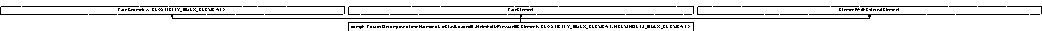
\includegraphics[height=0.491767cm]{classoomph_1_1FourierDecomposedTimeHarmonicLinElastLoadedByHelmholtzPressureBCElement}
\end{center}
\end{figure}
\subsection*{Public Member Functions}
\begin{DoxyCompactItemize}
\item 
\hyperlink{classoomph_1_1FourierDecomposedTimeHarmonicLinElastLoadedByHelmholtzPressureBCElement_aebbd02ebb45634d3e853669d7b37b6f3}{Fourier\+Decomposed\+Time\+Harmonic\+Lin\+Elast\+Loaded\+By\+Helmholtz\+Pressure\+B\+C\+Element} (\hyperlink{classoomph_1_1FiniteElement}{Finite\+Element} $\ast$const \&element\+\_\+pt, const int \&\hyperlink{classoomph_1_1FaceElement_a478d577ac6db67ecc80f1f02ae3ab170}{face\+\_\+index})
\begin{DoxyCompactList}\small\item\em Constructor, which takes a \char`\"{}bulk\char`\"{} element and the value of the index and its limit. \end{DoxyCompactList}\item 
void \hyperlink{classoomph_1_1FourierDecomposedTimeHarmonicLinElastLoadedByHelmholtzPressureBCElement_abf7b85b20e0a028a0179a64ad97acf1e}{fill\+\_\+in\+\_\+contribution\+\_\+to\+\_\+residuals} (\hyperlink{classoomph_1_1Vector}{Vector}$<$ double $>$ \&residuals)
\begin{DoxyCompactList}\small\item\em Return the residuals. \end{DoxyCompactList}\item 
void \hyperlink{classoomph_1_1FourierDecomposedTimeHarmonicLinElastLoadedByHelmholtzPressureBCElement_ac5f6369682a12573e07f07651ffb2a5f}{fill\+\_\+in\+\_\+contribution\+\_\+to\+\_\+jacobian} (\hyperlink{classoomph_1_1Vector}{Vector}$<$ double $>$ \&residuals, \hyperlink{classoomph_1_1DenseMatrix}{Dense\+Matrix}$<$ double $>$ \&jacobian)
\begin{DoxyCompactList}\small\item\em Fill in contribution from Jacobian. \end{DoxyCompactList}\item 
const double \& \hyperlink{classoomph_1_1FourierDecomposedTimeHarmonicLinElastLoadedByHelmholtzPressureBCElement_a874a6bc7470c0ba4de2b39f8444ed4e2}{q} () const
\begin{DoxyCompactList}\small\item\em Return the ratio of the stress scales used to non-\/dimensionalise the fluid and elasticity equations. E.\+g. $ Q = (\omega a)^2 \rho/E $, i.\+e. the ratio between the inertial fluid stress and the solid\textquotesingle{}s elastic modulus E. \end{DoxyCompactList}\item 
double $\ast$\& \hyperlink{classoomph_1_1FourierDecomposedTimeHarmonicLinElastLoadedByHelmholtzPressureBCElement_a3495996a8cdf7bb6e5ff5e3d9dcafa7e}{q\+\_\+pt} ()
\begin{DoxyCompactList}\small\item\em Return a pointer the ratio of stress scales used to non-\/dimensionalise the fluid and solid equations. \end{DoxyCompactList}\item 
void \hyperlink{classoomph_1_1FourierDecomposedTimeHarmonicLinElastLoadedByHelmholtzPressureBCElement_af1db6d117e79ceb536932adf64ea4752}{output} (std\+::ostream \&outfile)
\begin{DoxyCompactList}\small\item\em Output function. \end{DoxyCompactList}\item 
void \hyperlink{classoomph_1_1FourierDecomposedTimeHarmonicLinElastLoadedByHelmholtzPressureBCElement_a2c55e922cbc2a9f901356a47f696c0d6}{output} (std\+::ostream \&outfile, const unsigned \&n\+\_\+plot)
\begin{DoxyCompactList}\small\item\em Output function\+: Plot traction etc at \hyperlink{classoomph_1_1Gauss}{Gauss} points nplot is ignored. \end{DoxyCompactList}\item 
void \hyperlink{classoomph_1_1FourierDecomposedTimeHarmonicLinElastLoadedByHelmholtzPressureBCElement_a147a337796e4e10c43a956a85b441a5e}{output} (F\+I\+LE $\ast$file\+\_\+pt)
\begin{DoxyCompactList}\small\item\em C\+\_\+style output function. \end{DoxyCompactList}\item 
void \hyperlink{classoomph_1_1FourierDecomposedTimeHarmonicLinElastLoadedByHelmholtzPressureBCElement_a2383a2f19b7e45177f0a44f5d68fc2e9}{output} (F\+I\+LE $\ast$file\+\_\+pt, const unsigned \&n\+\_\+plot)
\begin{DoxyCompactList}\small\item\em C-\/style output function. \end{DoxyCompactList}\end{DoxyCompactItemize}
\subsection*{Protected Member Functions}
\begin{DoxyCompactItemize}
\item 
void \hyperlink{classoomph_1_1FourierDecomposedTimeHarmonicLinElastLoadedByHelmholtzPressureBCElement_abae27d4531220695eeb385c51ca0f82f}{fill\+\_\+in\+\_\+contribution\+\_\+to\+\_\+residuals\+\_\+helmholtz\+\_\+traction} (\hyperlink{classoomph_1_1Vector}{Vector}$<$ double $>$ \&residuals)
\begin{DoxyCompactList}\small\item\em Helper function that actually calculates the residuals. \end{DoxyCompactList}\end{DoxyCompactItemize}
\subsection*{Protected Attributes}
\begin{DoxyCompactItemize}
\item 
double $\ast$ \hyperlink{classoomph_1_1FourierDecomposedTimeHarmonicLinElastLoadedByHelmholtzPressureBCElement_ae9ffef6c7b99dcac84a59345b88e2938}{Q\+\_\+pt}
\begin{DoxyCompactList}\small\item\em Pointer to the ratio, $ Q $ , of the stress used to non-\/dimensionalise the fluid stresses to the stress used to non-\/dimensionalise the solid stresses. \end{DoxyCompactList}\item 
\hyperlink{classoomph_1_1Vector}{Vector}$<$ std\+::complex$<$ unsigned $>$ $>$ \hyperlink{classoomph_1_1FourierDecomposedTimeHarmonicLinElastLoadedByHelmholtzPressureBCElement_a662382c12e52846a2407ef5ec948d92b}{U\+\_\+index\+\_\+fourier\+\_\+decomposed\+\_\+time\+\_\+harmonic\+\_\+linear\+\_\+elasticity\+\_\+helmholtz\+\_\+traction}
\begin{DoxyCompactList}\small\item\em Index at which the i-\/th displacement component is stored. \end{DoxyCompactList}\end{DoxyCompactItemize}
\subsection*{Static Protected Attributes}
\begin{DoxyCompactItemize}
\item 
static double \hyperlink{classoomph_1_1FourierDecomposedTimeHarmonicLinElastLoadedByHelmholtzPressureBCElement_a6a24eef8286abb640d8edf3fa0f71e2c}{Default\+\_\+\+Q\+\_\+\+Value} =1.\+0
\begin{DoxyCompactList}\small\item\em Static default value for the ratio of stress scales used in the fluid and solid equations (default is 1.\+0) \end{DoxyCompactList}\end{DoxyCompactItemize}
\subsection*{Additional Inherited Members}


\subsection{Detailed Description}
\subsubsection*{template$<$class E\+L\+A\+S\+T\+I\+C\+I\+T\+Y\+\_\+\+B\+U\+L\+K\+\_\+\+E\+L\+E\+M\+E\+NT, class H\+E\+L\+M\+H\+O\+L\+T\+Z\+\_\+\+B\+U\+L\+K\+\_\+\+E\+L\+E\+M\+E\+NT$>$\newline
class oomph\+::\+Fourier\+Decomposed\+Time\+Harmonic\+Lin\+Elast\+Loaded\+By\+Helmholtz\+Pressure\+B\+C\+Element$<$ E\+L\+A\+S\+T\+I\+C\+I\+T\+Y\+\_\+\+B\+U\+L\+K\+\_\+\+E\+L\+E\+M\+E\+N\+T, H\+E\+L\+M\+H\+O\+L\+T\+Z\+\_\+\+B\+U\+L\+K\+\_\+\+E\+L\+E\+M\+E\+N\+T $>$}

A class for elements that allow the imposition of an applied traction in the equations of time-\/harmonic linear elasticity from a Helmholtz potential (interpreted as a displacement potential for the fluid in a quasi-\/steady, linearised F\+SI problem.) The geometrical information can be read from the Face\+Geometry$<$\+E\+L\+E\+M\+E\+N\+T$>$ class and and thus, we can be generic enough without the need to have a separate equations class. 

Definition at line 54 of file fourier\+\_\+decomposed\+\_\+helmholtz\+\_\+time\+\_\+harmonic\+\_\+linear\+\_\+elasticity\+\_\+interaction.\+h.



\subsection{Constructor \& Destructor Documentation}
\mbox{\Hypertarget{classoomph_1_1FourierDecomposedTimeHarmonicLinElastLoadedByHelmholtzPressureBCElement_aebbd02ebb45634d3e853669d7b37b6f3}\label{classoomph_1_1FourierDecomposedTimeHarmonicLinElastLoadedByHelmholtzPressureBCElement_aebbd02ebb45634d3e853669d7b37b6f3}} 
\index{oomph\+::\+Fourier\+Decomposed\+Time\+Harmonic\+Lin\+Elast\+Loaded\+By\+Helmholtz\+Pressure\+B\+C\+Element@{oomph\+::\+Fourier\+Decomposed\+Time\+Harmonic\+Lin\+Elast\+Loaded\+By\+Helmholtz\+Pressure\+B\+C\+Element}!Fourier\+Decomposed\+Time\+Harmonic\+Lin\+Elast\+Loaded\+By\+Helmholtz\+Pressure\+B\+C\+Element@{Fourier\+Decomposed\+Time\+Harmonic\+Lin\+Elast\+Loaded\+By\+Helmholtz\+Pressure\+B\+C\+Element}}
\index{Fourier\+Decomposed\+Time\+Harmonic\+Lin\+Elast\+Loaded\+By\+Helmholtz\+Pressure\+B\+C\+Element@{Fourier\+Decomposed\+Time\+Harmonic\+Lin\+Elast\+Loaded\+By\+Helmholtz\+Pressure\+B\+C\+Element}!oomph\+::\+Fourier\+Decomposed\+Time\+Harmonic\+Lin\+Elast\+Loaded\+By\+Helmholtz\+Pressure\+B\+C\+Element@{oomph\+::\+Fourier\+Decomposed\+Time\+Harmonic\+Lin\+Elast\+Loaded\+By\+Helmholtz\+Pressure\+B\+C\+Element}}
\subsubsection{\texorpdfstring{Fourier\+Decomposed\+Time\+Harmonic\+Lin\+Elast\+Loaded\+By\+Helmholtz\+Pressure\+B\+C\+Element()}{FourierDecomposedTimeHarmonicLinElastLoadedByHelmholtzPressureBCElement()}}
{\footnotesize\ttfamily template$<$class E\+L\+A\+S\+T\+I\+C\+I\+T\+Y\+\_\+\+B\+U\+L\+K\+\_\+\+E\+L\+E\+M\+E\+NT , class H\+E\+L\+M\+H\+O\+L\+T\+Z\+\_\+\+B\+U\+L\+K\+\_\+\+E\+L\+E\+M\+E\+NT $>$ \\
\hyperlink{classoomph_1_1FourierDecomposedTimeHarmonicLinElastLoadedByHelmholtzPressureBCElement}{oomph\+::\+Fourier\+Decomposed\+Time\+Harmonic\+Lin\+Elast\+Loaded\+By\+Helmholtz\+Pressure\+B\+C\+Element}$<$ E\+L\+A\+S\+T\+I\+C\+I\+T\+Y\+\_\+\+B\+U\+L\+K\+\_\+\+E\+L\+E\+M\+E\+NT, H\+E\+L\+M\+H\+O\+L\+T\+Z\+\_\+\+B\+U\+L\+K\+\_\+\+E\+L\+E\+M\+E\+NT $>$\+::\hyperlink{classoomph_1_1FourierDecomposedTimeHarmonicLinElastLoadedByHelmholtzPressureBCElement}{Fourier\+Decomposed\+Time\+Harmonic\+Lin\+Elast\+Loaded\+By\+Helmholtz\+Pressure\+B\+C\+Element} (\begin{DoxyParamCaption}\item[{\hyperlink{classoomph_1_1FiniteElement}{Finite\+Element} $\ast$const \&}]{element\+\_\+pt,  }\item[{const int \&}]{face\+\_\+index }\end{DoxyParamCaption})\hspace{0.3cm}{\ttfamily [inline]}}



Constructor, which takes a \char`\"{}bulk\char`\"{} element and the value of the index and its limit. 



Definition at line 86 of file fourier\+\_\+decomposed\+\_\+helmholtz\+\_\+time\+\_\+harmonic\+\_\+linear\+\_\+elasticity\+\_\+interaction.\+h.



References oomph\+::\+Finite\+Element\+::build\+\_\+face\+\_\+element(), oomph\+::\+Finite\+Element\+::has\+\_\+hanging\+\_\+nodes(), i, oomph\+::\+Finite\+Element\+::nodal\+\_\+dimension(), oomph\+::\+Element\+With\+External\+Element\+::set\+\_\+ninteraction(), and oomph\+::\+Fourier\+Decomposed\+Time\+Harmonic\+Lin\+Elast\+Loaded\+By\+Helmholtz\+Pressure\+B\+C\+Element$<$ E\+L\+A\+S\+T\+I\+C\+I\+T\+Y\+\_\+\+B\+U\+L\+K\+\_\+\+E\+L\+E\+M\+E\+N\+T, H\+E\+L\+M\+H\+O\+L\+T\+Z\+\_\+\+B\+U\+L\+K\+\_\+\+E\+L\+E\+M\+E\+N\+T $>$\+::\+U\+\_\+index\+\_\+fourier\+\_\+decomposed\+\_\+time\+\_\+harmonic\+\_\+linear\+\_\+elasticity\+\_\+helmholtz\+\_\+traction.



\subsection{Member Function Documentation}
\mbox{\Hypertarget{classoomph_1_1FourierDecomposedTimeHarmonicLinElastLoadedByHelmholtzPressureBCElement_ac5f6369682a12573e07f07651ffb2a5f}\label{classoomph_1_1FourierDecomposedTimeHarmonicLinElastLoadedByHelmholtzPressureBCElement_ac5f6369682a12573e07f07651ffb2a5f}} 
\index{oomph\+::\+Fourier\+Decomposed\+Time\+Harmonic\+Lin\+Elast\+Loaded\+By\+Helmholtz\+Pressure\+B\+C\+Element@{oomph\+::\+Fourier\+Decomposed\+Time\+Harmonic\+Lin\+Elast\+Loaded\+By\+Helmholtz\+Pressure\+B\+C\+Element}!fill\+\_\+in\+\_\+contribution\+\_\+to\+\_\+jacobian@{fill\+\_\+in\+\_\+contribution\+\_\+to\+\_\+jacobian}}
\index{fill\+\_\+in\+\_\+contribution\+\_\+to\+\_\+jacobian@{fill\+\_\+in\+\_\+contribution\+\_\+to\+\_\+jacobian}!oomph\+::\+Fourier\+Decomposed\+Time\+Harmonic\+Lin\+Elast\+Loaded\+By\+Helmholtz\+Pressure\+B\+C\+Element@{oomph\+::\+Fourier\+Decomposed\+Time\+Harmonic\+Lin\+Elast\+Loaded\+By\+Helmholtz\+Pressure\+B\+C\+Element}}
\subsubsection{\texorpdfstring{fill\+\_\+in\+\_\+contribution\+\_\+to\+\_\+jacobian()}{fill\_in\_contribution\_to\_jacobian()}}
{\footnotesize\ttfamily template$<$class E\+L\+A\+S\+T\+I\+C\+I\+T\+Y\+\_\+\+B\+U\+L\+K\+\_\+\+E\+L\+E\+M\+E\+NT , class H\+E\+L\+M\+H\+O\+L\+T\+Z\+\_\+\+B\+U\+L\+K\+\_\+\+E\+L\+E\+M\+E\+NT $>$ \\
void \hyperlink{classoomph_1_1FourierDecomposedTimeHarmonicLinElastLoadedByHelmholtzPressureBCElement}{oomph\+::\+Fourier\+Decomposed\+Time\+Harmonic\+Lin\+Elast\+Loaded\+By\+Helmholtz\+Pressure\+B\+C\+Element}$<$ E\+L\+A\+S\+T\+I\+C\+I\+T\+Y\+\_\+\+B\+U\+L\+K\+\_\+\+E\+L\+E\+M\+E\+NT, H\+E\+L\+M\+H\+O\+L\+T\+Z\+\_\+\+B\+U\+L\+K\+\_\+\+E\+L\+E\+M\+E\+NT $>$\+::fill\+\_\+in\+\_\+contribution\+\_\+to\+\_\+jacobian (\begin{DoxyParamCaption}\item[{\hyperlink{classoomph_1_1Vector}{Vector}$<$ double $>$ \&}]{residuals,  }\item[{\hyperlink{classoomph_1_1DenseMatrix}{Dense\+Matrix}$<$ double $>$ \&}]{jacobian }\end{DoxyParamCaption})\hspace{0.3cm}{\ttfamily [inline]}, {\ttfamily [virtual]}}



Fill in contribution from Jacobian. 



Reimplemented from \hyperlink{classoomph_1_1ElementWithExternalElement_ae5fb09552a8271e891438f8d058ca1b8}{oomph\+::\+Element\+With\+External\+Element}.



Definition at line 150 of file fourier\+\_\+decomposed\+\_\+helmholtz\+\_\+time\+\_\+harmonic\+\_\+linear\+\_\+elasticity\+\_\+interaction.\+h.



References oomph\+::\+Fourier\+Decomposed\+Time\+Harmonic\+Lin\+Elast\+Loaded\+By\+Helmholtz\+Pressure\+B\+C\+Element$<$ E\+L\+A\+S\+T\+I\+C\+I\+T\+Y\+\_\+\+B\+U\+L\+K\+\_\+\+E\+L\+E\+M\+E\+N\+T, H\+E\+L\+M\+H\+O\+L\+T\+Z\+\_\+\+B\+U\+L\+K\+\_\+\+E\+L\+E\+M\+E\+N\+T $>$\+::fill\+\_\+in\+\_\+contribution\+\_\+to\+\_\+residuals\+\_\+helmholtz\+\_\+traction(), and oomph\+::\+Element\+With\+External\+Element\+::fill\+\_\+in\+\_\+jacobian\+\_\+from\+\_\+external\+\_\+interaction\+\_\+by\+\_\+fd().

\mbox{\Hypertarget{classoomph_1_1FourierDecomposedTimeHarmonicLinElastLoadedByHelmholtzPressureBCElement_abf7b85b20e0a028a0179a64ad97acf1e}\label{classoomph_1_1FourierDecomposedTimeHarmonicLinElastLoadedByHelmholtzPressureBCElement_abf7b85b20e0a028a0179a64ad97acf1e}} 
\index{oomph\+::\+Fourier\+Decomposed\+Time\+Harmonic\+Lin\+Elast\+Loaded\+By\+Helmholtz\+Pressure\+B\+C\+Element@{oomph\+::\+Fourier\+Decomposed\+Time\+Harmonic\+Lin\+Elast\+Loaded\+By\+Helmholtz\+Pressure\+B\+C\+Element}!fill\+\_\+in\+\_\+contribution\+\_\+to\+\_\+residuals@{fill\+\_\+in\+\_\+contribution\+\_\+to\+\_\+residuals}}
\index{fill\+\_\+in\+\_\+contribution\+\_\+to\+\_\+residuals@{fill\+\_\+in\+\_\+contribution\+\_\+to\+\_\+residuals}!oomph\+::\+Fourier\+Decomposed\+Time\+Harmonic\+Lin\+Elast\+Loaded\+By\+Helmholtz\+Pressure\+B\+C\+Element@{oomph\+::\+Fourier\+Decomposed\+Time\+Harmonic\+Lin\+Elast\+Loaded\+By\+Helmholtz\+Pressure\+B\+C\+Element}}
\subsubsection{\texorpdfstring{fill\+\_\+in\+\_\+contribution\+\_\+to\+\_\+residuals()}{fill\_in\_contribution\_to\_residuals()}}
{\footnotesize\ttfamily template$<$class E\+L\+A\+S\+T\+I\+C\+I\+T\+Y\+\_\+\+B\+U\+L\+K\+\_\+\+E\+L\+E\+M\+E\+NT , class H\+E\+L\+M\+H\+O\+L\+T\+Z\+\_\+\+B\+U\+L\+K\+\_\+\+E\+L\+E\+M\+E\+NT $>$ \\
void \hyperlink{classoomph_1_1FourierDecomposedTimeHarmonicLinElastLoadedByHelmholtzPressureBCElement}{oomph\+::\+Fourier\+Decomposed\+Time\+Harmonic\+Lin\+Elast\+Loaded\+By\+Helmholtz\+Pressure\+B\+C\+Element}$<$ E\+L\+A\+S\+T\+I\+C\+I\+T\+Y\+\_\+\+B\+U\+L\+K\+\_\+\+E\+L\+E\+M\+E\+NT, H\+E\+L\+M\+H\+O\+L\+T\+Z\+\_\+\+B\+U\+L\+K\+\_\+\+E\+L\+E\+M\+E\+NT $>$\+::fill\+\_\+in\+\_\+contribution\+\_\+to\+\_\+residuals (\begin{DoxyParamCaption}\item[{\hyperlink{classoomph_1_1Vector}{Vector}$<$ double $>$ \&}]{residuals }\end{DoxyParamCaption})\hspace{0.3cm}{\ttfamily [inline]}, {\ttfamily [virtual]}}



Return the residuals. 



Reimplemented from \hyperlink{classoomph_1_1GeneralisedElement_a310c97f515e8504a48179c0e72c550d7}{oomph\+::\+Generalised\+Element}.



Definition at line 142 of file fourier\+\_\+decomposed\+\_\+helmholtz\+\_\+time\+\_\+harmonic\+\_\+linear\+\_\+elasticity\+\_\+interaction.\+h.



References oomph\+::\+Fourier\+Decomposed\+Time\+Harmonic\+Lin\+Elast\+Loaded\+By\+Helmholtz\+Pressure\+B\+C\+Element$<$ E\+L\+A\+S\+T\+I\+C\+I\+T\+Y\+\_\+\+B\+U\+L\+K\+\_\+\+E\+L\+E\+M\+E\+N\+T, H\+E\+L\+M\+H\+O\+L\+T\+Z\+\_\+\+B\+U\+L\+K\+\_\+\+E\+L\+E\+M\+E\+N\+T $>$\+::fill\+\_\+in\+\_\+contribution\+\_\+to\+\_\+residuals\+\_\+helmholtz\+\_\+traction().

\mbox{\Hypertarget{classoomph_1_1FourierDecomposedTimeHarmonicLinElastLoadedByHelmholtzPressureBCElement_abae27d4531220695eeb385c51ca0f82f}\label{classoomph_1_1FourierDecomposedTimeHarmonicLinElastLoadedByHelmholtzPressureBCElement_abae27d4531220695eeb385c51ca0f82f}} 
\index{oomph\+::\+Fourier\+Decomposed\+Time\+Harmonic\+Lin\+Elast\+Loaded\+By\+Helmholtz\+Pressure\+B\+C\+Element@{oomph\+::\+Fourier\+Decomposed\+Time\+Harmonic\+Lin\+Elast\+Loaded\+By\+Helmholtz\+Pressure\+B\+C\+Element}!fill\+\_\+in\+\_\+contribution\+\_\+to\+\_\+residuals\+\_\+helmholtz\+\_\+traction@{fill\+\_\+in\+\_\+contribution\+\_\+to\+\_\+residuals\+\_\+helmholtz\+\_\+traction}}
\index{fill\+\_\+in\+\_\+contribution\+\_\+to\+\_\+residuals\+\_\+helmholtz\+\_\+traction@{fill\+\_\+in\+\_\+contribution\+\_\+to\+\_\+residuals\+\_\+helmholtz\+\_\+traction}!oomph\+::\+Fourier\+Decomposed\+Time\+Harmonic\+Lin\+Elast\+Loaded\+By\+Helmholtz\+Pressure\+B\+C\+Element@{oomph\+::\+Fourier\+Decomposed\+Time\+Harmonic\+Lin\+Elast\+Loaded\+By\+Helmholtz\+Pressure\+B\+C\+Element}}
\subsubsection{\texorpdfstring{fill\+\_\+in\+\_\+contribution\+\_\+to\+\_\+residuals\+\_\+helmholtz\+\_\+traction()}{fill\_in\_contribution\_to\_residuals\_helmholtz\_traction()}}
{\footnotesize\ttfamily template$<$class E\+L\+A\+S\+T\+I\+C\+I\+T\+Y\+\_\+\+B\+U\+L\+K\+\_\+\+E\+L\+E\+M\+E\+NT , class H\+E\+L\+M\+H\+O\+L\+T\+Z\+\_\+\+B\+U\+L\+K\+\_\+\+E\+L\+E\+M\+E\+NT $>$ \\
void \hyperlink{classoomph_1_1FourierDecomposedTimeHarmonicLinElastLoadedByHelmholtzPressureBCElement}{oomph\+::\+Fourier\+Decomposed\+Time\+Harmonic\+Lin\+Elast\+Loaded\+By\+Helmholtz\+Pressure\+B\+C\+Element}$<$ E\+L\+A\+S\+T\+I\+C\+I\+T\+Y\+\_\+\+B\+U\+L\+K\+\_\+\+E\+L\+E\+M\+E\+NT, H\+E\+L\+M\+H\+O\+L\+T\+Z\+\_\+\+B\+U\+L\+K\+\_\+\+E\+L\+E\+M\+E\+NT $>$\+::fill\+\_\+in\+\_\+contribution\+\_\+to\+\_\+residuals\+\_\+helmholtz\+\_\+traction (\begin{DoxyParamCaption}\item[{\hyperlink{classoomph_1_1Vector}{Vector}$<$ double $>$ \&}]{residuals }\end{DoxyParamCaption})\hspace{0.3cm}{\ttfamily [protected]}}



Helper function that actually calculates the residuals. 

Return the residuals. 

Definition at line 269 of file fourier\+\_\+decomposed\+\_\+helmholtz\+\_\+time\+\_\+harmonic\+\_\+linear\+\_\+elasticity\+\_\+interaction.\+h.



References oomph\+::\+Finite\+Element\+::dshape\+\_\+local\+\_\+at\+\_\+knot(), oomph\+::\+Element\+With\+External\+Element\+::external\+\_\+element\+\_\+local\+\_\+coord(), oomph\+::\+Element\+With\+External\+Element\+::external\+\_\+element\+\_\+pt(), i, oomph\+::\+Finite\+Element\+::integral\+\_\+pt(), oomph\+::\+Face\+Element\+::interpolated\+\_\+x(), oomph\+::\+Finite\+Element\+::nnodal\+\_\+position\+\_\+type(), oomph\+::\+Finite\+Element\+::nnode(), oomph\+::\+Finite\+Element\+::nodal\+\_\+dimension(), oomph\+::\+Finite\+Element\+::nodal\+\_\+local\+\_\+eqn(), oomph\+::\+Finite\+Element\+::nodal\+\_\+position(), oomph\+::\+Integral\+::nweight(), oomph\+::\+Face\+Element\+::outer\+\_\+unit\+\_\+normal(), oomph\+::\+Fourier\+Decomposed\+Time\+Harmonic\+Lin\+Elast\+Loaded\+By\+Helmholtz\+Pressure\+B\+C\+Element$<$ E\+L\+A\+S\+T\+I\+C\+I\+T\+Y\+\_\+\+B\+U\+L\+K\+\_\+\+E\+L\+E\+M\+E\+N\+T, H\+E\+L\+M\+H\+O\+L\+T\+Z\+\_\+\+B\+U\+L\+K\+\_\+\+E\+L\+E\+M\+E\+N\+T $>$\+::q(), oomph\+::\+Fourier\+Decomposed\+Time\+Harmonic\+Lin\+Elast\+Loaded\+By\+Helmholtz\+Pressure\+B\+C\+Element$<$ E\+L\+A\+S\+T\+I\+C\+I\+T\+Y\+\_\+\+B\+U\+L\+K\+\_\+\+E\+L\+E\+M\+E\+N\+T, H\+E\+L\+M\+H\+O\+L\+T\+Z\+\_\+\+B\+U\+L\+K\+\_\+\+E\+L\+E\+M\+E\+N\+T $>$\+::\+U\+\_\+index\+\_\+fourier\+\_\+decomposed\+\_\+time\+\_\+harmonic\+\_\+linear\+\_\+elasticity\+\_\+helmholtz\+\_\+traction, oomph\+::\+Quad\+Tree\+Names\+::W, and oomph\+::\+Integral\+::weight().



Referenced by oomph\+::\+Fourier\+Decomposed\+Time\+Harmonic\+Lin\+Elast\+Loaded\+By\+Helmholtz\+Pressure\+B\+C\+Element$<$ E\+L\+A\+S\+T\+I\+C\+I\+T\+Y\+\_\+\+B\+U\+L\+K\+\_\+\+E\+L\+E\+M\+E\+N\+T, H\+E\+L\+M\+H\+O\+L\+T\+Z\+\_\+\+B\+U\+L\+K\+\_\+\+E\+L\+E\+M\+E\+N\+T $>$\+::fill\+\_\+in\+\_\+contribution\+\_\+to\+\_\+jacobian(), oomph\+::\+Fourier\+Decomposed\+Time\+Harmonic\+Lin\+Elast\+Loaded\+By\+Helmholtz\+Pressure\+B\+C\+Element$<$ E\+L\+A\+S\+T\+I\+C\+I\+T\+Y\+\_\+\+B\+U\+L\+K\+\_\+\+E\+L\+E\+M\+E\+N\+T, H\+E\+L\+M\+H\+O\+L\+T\+Z\+\_\+\+B\+U\+L\+K\+\_\+\+E\+L\+E\+M\+E\+N\+T $>$\+::fill\+\_\+in\+\_\+contribution\+\_\+to\+\_\+residuals(), and oomph\+::\+Fourier\+Decomposed\+Time\+Harmonic\+Lin\+Elast\+Loaded\+By\+Helmholtz\+Pressure\+B\+C\+Element$<$ E\+L\+A\+S\+T\+I\+C\+I\+T\+Y\+\_\+\+B\+U\+L\+K\+\_\+\+E\+L\+E\+M\+E\+N\+T, H\+E\+L\+M\+H\+O\+L\+T\+Z\+\_\+\+B\+U\+L\+K\+\_\+\+E\+L\+E\+M\+E\+N\+T $>$\+::output().

\mbox{\Hypertarget{classoomph_1_1FourierDecomposedTimeHarmonicLinElastLoadedByHelmholtzPressureBCElement_af1db6d117e79ceb536932adf64ea4752}\label{classoomph_1_1FourierDecomposedTimeHarmonicLinElastLoadedByHelmholtzPressureBCElement_af1db6d117e79ceb536932adf64ea4752}} 
\index{oomph\+::\+Fourier\+Decomposed\+Time\+Harmonic\+Lin\+Elast\+Loaded\+By\+Helmholtz\+Pressure\+B\+C\+Element@{oomph\+::\+Fourier\+Decomposed\+Time\+Harmonic\+Lin\+Elast\+Loaded\+By\+Helmholtz\+Pressure\+B\+C\+Element}!output@{output}}
\index{output@{output}!oomph\+::\+Fourier\+Decomposed\+Time\+Harmonic\+Lin\+Elast\+Loaded\+By\+Helmholtz\+Pressure\+B\+C\+Element@{oomph\+::\+Fourier\+Decomposed\+Time\+Harmonic\+Lin\+Elast\+Loaded\+By\+Helmholtz\+Pressure\+B\+C\+Element}}
\subsubsection{\texorpdfstring{output()}{output()}\hspace{0.1cm}{\footnotesize\ttfamily [1/4]}}
{\footnotesize\ttfamily template$<$class E\+L\+A\+S\+T\+I\+C\+I\+T\+Y\+\_\+\+B\+U\+L\+K\+\_\+\+E\+L\+E\+M\+E\+NT , class H\+E\+L\+M\+H\+O\+L\+T\+Z\+\_\+\+B\+U\+L\+K\+\_\+\+E\+L\+E\+M\+E\+NT $>$ \\
void \hyperlink{classoomph_1_1FourierDecomposedTimeHarmonicLinElastLoadedByHelmholtzPressureBCElement}{oomph\+::\+Fourier\+Decomposed\+Time\+Harmonic\+Lin\+Elast\+Loaded\+By\+Helmholtz\+Pressure\+B\+C\+Element}$<$ E\+L\+A\+S\+T\+I\+C\+I\+T\+Y\+\_\+\+B\+U\+L\+K\+\_\+\+E\+L\+E\+M\+E\+NT, H\+E\+L\+M\+H\+O\+L\+T\+Z\+\_\+\+B\+U\+L\+K\+\_\+\+E\+L\+E\+M\+E\+NT $>$\+::output (\begin{DoxyParamCaption}\item[{std\+::ostream \&}]{outfile }\end{DoxyParamCaption})\hspace{0.3cm}{\ttfamily [inline]}, {\ttfamily [virtual]}}



Output function. 

Dummy 

Reimplemented from \hyperlink{classoomph_1_1FiniteElement_a2ad98a3d2ef4999f1bef62c0ff13f2a7}{oomph\+::\+Finite\+Element}.



Definition at line 173 of file fourier\+\_\+decomposed\+\_\+helmholtz\+\_\+time\+\_\+harmonic\+\_\+linear\+\_\+elasticity\+\_\+interaction.\+h.



Referenced by oomph\+::\+Fourier\+Decomposed\+Helmholtz\+Flux\+From\+Normal\+Displacement\+B\+C\+Element$<$ H\+E\+L\+M\+H\+O\+L\+T\+Z\+\_\+\+B\+U\+L\+K\+\_\+\+E\+L\+E\+M\+E\+N\+T, E\+L\+A\+S\+T\+I\+C\+I\+T\+Y\+\_\+\+B\+U\+L\+K\+\_\+\+E\+L\+E\+M\+E\+N\+T $>$\+::output().

\mbox{\Hypertarget{classoomph_1_1FourierDecomposedTimeHarmonicLinElastLoadedByHelmholtzPressureBCElement_a2c55e922cbc2a9f901356a47f696c0d6}\label{classoomph_1_1FourierDecomposedTimeHarmonicLinElastLoadedByHelmholtzPressureBCElement_a2c55e922cbc2a9f901356a47f696c0d6}} 
\index{oomph\+::\+Fourier\+Decomposed\+Time\+Harmonic\+Lin\+Elast\+Loaded\+By\+Helmholtz\+Pressure\+B\+C\+Element@{oomph\+::\+Fourier\+Decomposed\+Time\+Harmonic\+Lin\+Elast\+Loaded\+By\+Helmholtz\+Pressure\+B\+C\+Element}!output@{output}}
\index{output@{output}!oomph\+::\+Fourier\+Decomposed\+Time\+Harmonic\+Lin\+Elast\+Loaded\+By\+Helmholtz\+Pressure\+B\+C\+Element@{oomph\+::\+Fourier\+Decomposed\+Time\+Harmonic\+Lin\+Elast\+Loaded\+By\+Helmholtz\+Pressure\+B\+C\+Element}}
\subsubsection{\texorpdfstring{output()}{output()}\hspace{0.1cm}{\footnotesize\ttfamily [2/4]}}
{\footnotesize\ttfamily template$<$class E\+L\+A\+S\+T\+I\+C\+I\+T\+Y\+\_\+\+B\+U\+L\+K\+\_\+\+E\+L\+E\+M\+E\+NT , class H\+E\+L\+M\+H\+O\+L\+T\+Z\+\_\+\+B\+U\+L\+K\+\_\+\+E\+L\+E\+M\+E\+NT $>$ \\
void \hyperlink{classoomph_1_1FourierDecomposedTimeHarmonicLinElastLoadedByHelmholtzPressureBCElement}{oomph\+::\+Fourier\+Decomposed\+Time\+Harmonic\+Lin\+Elast\+Loaded\+By\+Helmholtz\+Pressure\+B\+C\+Element}$<$ E\+L\+A\+S\+T\+I\+C\+I\+T\+Y\+\_\+\+B\+U\+L\+K\+\_\+\+E\+L\+E\+M\+E\+NT, H\+E\+L\+M\+H\+O\+L\+T\+Z\+\_\+\+B\+U\+L\+K\+\_\+\+E\+L\+E\+M\+E\+NT $>$\+::output (\begin{DoxyParamCaption}\item[{std\+::ostream \&}]{outfile,  }\item[{const unsigned \&}]{n\+\_\+plot }\end{DoxyParamCaption})\hspace{0.3cm}{\ttfamily [inline]}, {\ttfamily [virtual]}}



Output function\+: Plot traction etc at \hyperlink{classoomph_1_1Gauss}{Gauss} points nplot is ignored. 



Reimplemented from \hyperlink{classoomph_1_1FiniteElement_afa9d9b2670f999b43e6679c9dd28c457}{oomph\+::\+Finite\+Element}.



Definition at line 182 of file fourier\+\_\+decomposed\+\_\+helmholtz\+\_\+time\+\_\+harmonic\+\_\+linear\+\_\+elasticity\+\_\+interaction.\+h.



References oomph\+::\+Element\+With\+External\+Element\+::external\+\_\+element\+\_\+local\+\_\+coord(), oomph\+::\+Element\+With\+External\+Element\+::external\+\_\+element\+\_\+pt(), i, oomph\+::\+Finite\+Element\+::integral\+\_\+pt(), oomph\+::\+Finite\+Element\+::interpolated\+\_\+zeta(), oomph\+::\+Integral\+::knot(), oomph\+::\+Finite\+Element\+::nodal\+\_\+dimension(), oomph\+::\+Integral\+::nweight(), oomph\+::\+Face\+Element\+::outer\+\_\+unit\+\_\+normal(), and oomph\+::\+Fourier\+Decomposed\+Time\+Harmonic\+Lin\+Elast\+Loaded\+By\+Helmholtz\+Pressure\+B\+C\+Element$<$ E\+L\+A\+S\+T\+I\+C\+I\+T\+Y\+\_\+\+B\+U\+L\+K\+\_\+\+E\+L\+E\+M\+E\+N\+T, H\+E\+L\+M\+H\+O\+L\+T\+Z\+\_\+\+B\+U\+L\+K\+\_\+\+E\+L\+E\+M\+E\+N\+T $>$\+::q().

\mbox{\Hypertarget{classoomph_1_1FourierDecomposedTimeHarmonicLinElastLoadedByHelmholtzPressureBCElement_a147a337796e4e10c43a956a85b441a5e}\label{classoomph_1_1FourierDecomposedTimeHarmonicLinElastLoadedByHelmholtzPressureBCElement_a147a337796e4e10c43a956a85b441a5e}} 
\index{oomph\+::\+Fourier\+Decomposed\+Time\+Harmonic\+Lin\+Elast\+Loaded\+By\+Helmholtz\+Pressure\+B\+C\+Element@{oomph\+::\+Fourier\+Decomposed\+Time\+Harmonic\+Lin\+Elast\+Loaded\+By\+Helmholtz\+Pressure\+B\+C\+Element}!output@{output}}
\index{output@{output}!oomph\+::\+Fourier\+Decomposed\+Time\+Harmonic\+Lin\+Elast\+Loaded\+By\+Helmholtz\+Pressure\+B\+C\+Element@{oomph\+::\+Fourier\+Decomposed\+Time\+Harmonic\+Lin\+Elast\+Loaded\+By\+Helmholtz\+Pressure\+B\+C\+Element}}
\subsubsection{\texorpdfstring{output()}{output()}\hspace{0.1cm}{\footnotesize\ttfamily [3/4]}}
{\footnotesize\ttfamily template$<$class E\+L\+A\+S\+T\+I\+C\+I\+T\+Y\+\_\+\+B\+U\+L\+K\+\_\+\+E\+L\+E\+M\+E\+NT , class H\+E\+L\+M\+H\+O\+L\+T\+Z\+\_\+\+B\+U\+L\+K\+\_\+\+E\+L\+E\+M\+E\+NT $>$ \\
void \hyperlink{classoomph_1_1FourierDecomposedTimeHarmonicLinElastLoadedByHelmholtzPressureBCElement}{oomph\+::\+Fourier\+Decomposed\+Time\+Harmonic\+Lin\+Elast\+Loaded\+By\+Helmholtz\+Pressure\+B\+C\+Element}$<$ E\+L\+A\+S\+T\+I\+C\+I\+T\+Y\+\_\+\+B\+U\+L\+K\+\_\+\+E\+L\+E\+M\+E\+NT, H\+E\+L\+M\+H\+O\+L\+T\+Z\+\_\+\+B\+U\+L\+K\+\_\+\+E\+L\+E\+M\+E\+NT $>$\+::output (\begin{DoxyParamCaption}\item[{F\+I\+LE $\ast$}]{file\+\_\+pt }\end{DoxyParamCaption})\hspace{0.3cm}{\ttfamily [inline]}, {\ttfamily [virtual]}}



C\+\_\+style output function. 



Reimplemented from \hyperlink{classoomph_1_1FiniteElement_a72cddd09f8ddbee1a20a1ff404c6943e}{oomph\+::\+Finite\+Element}.



Definition at line 239 of file fourier\+\_\+decomposed\+\_\+helmholtz\+\_\+time\+\_\+harmonic\+\_\+linear\+\_\+elasticity\+\_\+interaction.\+h.



References oomph\+::output().

\mbox{\Hypertarget{classoomph_1_1FourierDecomposedTimeHarmonicLinElastLoadedByHelmholtzPressureBCElement_a2383a2f19b7e45177f0a44f5d68fc2e9}\label{classoomph_1_1FourierDecomposedTimeHarmonicLinElastLoadedByHelmholtzPressureBCElement_a2383a2f19b7e45177f0a44f5d68fc2e9}} 
\index{oomph\+::\+Fourier\+Decomposed\+Time\+Harmonic\+Lin\+Elast\+Loaded\+By\+Helmholtz\+Pressure\+B\+C\+Element@{oomph\+::\+Fourier\+Decomposed\+Time\+Harmonic\+Lin\+Elast\+Loaded\+By\+Helmholtz\+Pressure\+B\+C\+Element}!output@{output}}
\index{output@{output}!oomph\+::\+Fourier\+Decomposed\+Time\+Harmonic\+Lin\+Elast\+Loaded\+By\+Helmholtz\+Pressure\+B\+C\+Element@{oomph\+::\+Fourier\+Decomposed\+Time\+Harmonic\+Lin\+Elast\+Loaded\+By\+Helmholtz\+Pressure\+B\+C\+Element}}
\subsubsection{\texorpdfstring{output()}{output()}\hspace{0.1cm}{\footnotesize\ttfamily [4/4]}}
{\footnotesize\ttfamily template$<$class E\+L\+A\+S\+T\+I\+C\+I\+T\+Y\+\_\+\+B\+U\+L\+K\+\_\+\+E\+L\+E\+M\+E\+NT , class H\+E\+L\+M\+H\+O\+L\+T\+Z\+\_\+\+B\+U\+L\+K\+\_\+\+E\+L\+E\+M\+E\+NT $>$ \\
void \hyperlink{classoomph_1_1FourierDecomposedTimeHarmonicLinElastLoadedByHelmholtzPressureBCElement}{oomph\+::\+Fourier\+Decomposed\+Time\+Harmonic\+Lin\+Elast\+Loaded\+By\+Helmholtz\+Pressure\+B\+C\+Element}$<$ E\+L\+A\+S\+T\+I\+C\+I\+T\+Y\+\_\+\+B\+U\+L\+K\+\_\+\+E\+L\+E\+M\+E\+NT, H\+E\+L\+M\+H\+O\+L\+T\+Z\+\_\+\+B\+U\+L\+K\+\_\+\+E\+L\+E\+M\+E\+NT $>$\+::output (\begin{DoxyParamCaption}\item[{F\+I\+LE $\ast$}]{file\+\_\+pt,  }\item[{const unsigned \&}]{n\+\_\+plot }\end{DoxyParamCaption})\hspace{0.3cm}{\ttfamily [inline]}, {\ttfamily [virtual]}}



C-\/style output function. 



Reimplemented from \hyperlink{classoomph_1_1FiniteElement_adfaee690bb0608f03320eeb9d110d48c}{oomph\+::\+Finite\+Element}.



Definition at line 243 of file fourier\+\_\+decomposed\+\_\+helmholtz\+\_\+time\+\_\+harmonic\+\_\+linear\+\_\+elasticity\+\_\+interaction.\+h.



References oomph\+::\+Fourier\+Decomposed\+Time\+Harmonic\+Lin\+Elast\+Loaded\+By\+Helmholtz\+Pressure\+B\+C\+Element$<$ E\+L\+A\+S\+T\+I\+C\+I\+T\+Y\+\_\+\+B\+U\+L\+K\+\_\+\+E\+L\+E\+M\+E\+N\+T, H\+E\+L\+M\+H\+O\+L\+T\+Z\+\_\+\+B\+U\+L\+K\+\_\+\+E\+L\+E\+M\+E\+N\+T $>$\+::\+Default\+\_\+\+Q\+\_\+\+Value, oomph\+::\+Fourier\+Decomposed\+Time\+Harmonic\+Lin\+Elast\+Loaded\+By\+Helmholtz\+Pressure\+B\+C\+Element$<$ E\+L\+A\+S\+T\+I\+C\+I\+T\+Y\+\_\+\+B\+U\+L\+K\+\_\+\+E\+L\+E\+M\+E\+N\+T, H\+E\+L\+M\+H\+O\+L\+T\+Z\+\_\+\+B\+U\+L\+K\+\_\+\+E\+L\+E\+M\+E\+N\+T $>$\+::fill\+\_\+in\+\_\+contribution\+\_\+to\+\_\+residuals\+\_\+helmholtz\+\_\+traction(), and oomph\+::output().

\mbox{\Hypertarget{classoomph_1_1FourierDecomposedTimeHarmonicLinElastLoadedByHelmholtzPressureBCElement_a874a6bc7470c0ba4de2b39f8444ed4e2}\label{classoomph_1_1FourierDecomposedTimeHarmonicLinElastLoadedByHelmholtzPressureBCElement_a874a6bc7470c0ba4de2b39f8444ed4e2}} 
\index{oomph\+::\+Fourier\+Decomposed\+Time\+Harmonic\+Lin\+Elast\+Loaded\+By\+Helmholtz\+Pressure\+B\+C\+Element@{oomph\+::\+Fourier\+Decomposed\+Time\+Harmonic\+Lin\+Elast\+Loaded\+By\+Helmholtz\+Pressure\+B\+C\+Element}!q@{q}}
\index{q@{q}!oomph\+::\+Fourier\+Decomposed\+Time\+Harmonic\+Lin\+Elast\+Loaded\+By\+Helmholtz\+Pressure\+B\+C\+Element@{oomph\+::\+Fourier\+Decomposed\+Time\+Harmonic\+Lin\+Elast\+Loaded\+By\+Helmholtz\+Pressure\+B\+C\+Element}}
\subsubsection{\texorpdfstring{q()}{q()}}
{\footnotesize\ttfamily template$<$class E\+L\+A\+S\+T\+I\+C\+I\+T\+Y\+\_\+\+B\+U\+L\+K\+\_\+\+E\+L\+E\+M\+E\+NT , class H\+E\+L\+M\+H\+O\+L\+T\+Z\+\_\+\+B\+U\+L\+K\+\_\+\+E\+L\+E\+M\+E\+NT $>$ \\
const double\& \hyperlink{classoomph_1_1FourierDecomposedTimeHarmonicLinElastLoadedByHelmholtzPressureBCElement}{oomph\+::\+Fourier\+Decomposed\+Time\+Harmonic\+Lin\+Elast\+Loaded\+By\+Helmholtz\+Pressure\+B\+C\+Element}$<$ E\+L\+A\+S\+T\+I\+C\+I\+T\+Y\+\_\+\+B\+U\+L\+K\+\_\+\+E\+L\+E\+M\+E\+NT, H\+E\+L\+M\+H\+O\+L\+T\+Z\+\_\+\+B\+U\+L\+K\+\_\+\+E\+L\+E\+M\+E\+NT $>$\+::q (\begin{DoxyParamCaption}{ }\end{DoxyParamCaption}) const\hspace{0.3cm}{\ttfamily [inline]}}



Return the ratio of the stress scales used to non-\/dimensionalise the fluid and elasticity equations. E.\+g. $ Q = (\omega a)^2 \rho/E $, i.\+e. the ratio between the inertial fluid stress and the solid\textquotesingle{}s elastic modulus E. 



Definition at line 165 of file fourier\+\_\+decomposed\+\_\+helmholtz\+\_\+time\+\_\+harmonic\+\_\+linear\+\_\+elasticity\+\_\+interaction.\+h.



References oomph\+::\+Fourier\+Decomposed\+Time\+Harmonic\+Lin\+Elast\+Loaded\+By\+Helmholtz\+Pressure\+B\+C\+Element$<$ E\+L\+A\+S\+T\+I\+C\+I\+T\+Y\+\_\+\+B\+U\+L\+K\+\_\+\+E\+L\+E\+M\+E\+N\+T, H\+E\+L\+M\+H\+O\+L\+T\+Z\+\_\+\+B\+U\+L\+K\+\_\+\+E\+L\+E\+M\+E\+N\+T $>$\+::\+Q\+\_\+pt.



Referenced by oomph\+::\+Fourier\+Decomposed\+Time\+Harmonic\+Lin\+Elast\+Loaded\+By\+Helmholtz\+Pressure\+B\+C\+Element$<$ E\+L\+A\+S\+T\+I\+C\+I\+T\+Y\+\_\+\+B\+U\+L\+K\+\_\+\+E\+L\+E\+M\+E\+N\+T, H\+E\+L\+M\+H\+O\+L\+T\+Z\+\_\+\+B\+U\+L\+K\+\_\+\+E\+L\+E\+M\+E\+N\+T $>$\+::fill\+\_\+in\+\_\+contribution\+\_\+to\+\_\+residuals\+\_\+helmholtz\+\_\+traction(), and oomph\+::\+Fourier\+Decomposed\+Time\+Harmonic\+Lin\+Elast\+Loaded\+By\+Helmholtz\+Pressure\+B\+C\+Element$<$ E\+L\+A\+S\+T\+I\+C\+I\+T\+Y\+\_\+\+B\+U\+L\+K\+\_\+\+E\+L\+E\+M\+E\+N\+T, H\+E\+L\+M\+H\+O\+L\+T\+Z\+\_\+\+B\+U\+L\+K\+\_\+\+E\+L\+E\+M\+E\+N\+T $>$\+::output().

\mbox{\Hypertarget{classoomph_1_1FourierDecomposedTimeHarmonicLinElastLoadedByHelmholtzPressureBCElement_a3495996a8cdf7bb6e5ff5e3d9dcafa7e}\label{classoomph_1_1FourierDecomposedTimeHarmonicLinElastLoadedByHelmholtzPressureBCElement_a3495996a8cdf7bb6e5ff5e3d9dcafa7e}} 
\index{oomph\+::\+Fourier\+Decomposed\+Time\+Harmonic\+Lin\+Elast\+Loaded\+By\+Helmholtz\+Pressure\+B\+C\+Element@{oomph\+::\+Fourier\+Decomposed\+Time\+Harmonic\+Lin\+Elast\+Loaded\+By\+Helmholtz\+Pressure\+B\+C\+Element}!q\+\_\+pt@{q\+\_\+pt}}
\index{q\+\_\+pt@{q\+\_\+pt}!oomph\+::\+Fourier\+Decomposed\+Time\+Harmonic\+Lin\+Elast\+Loaded\+By\+Helmholtz\+Pressure\+B\+C\+Element@{oomph\+::\+Fourier\+Decomposed\+Time\+Harmonic\+Lin\+Elast\+Loaded\+By\+Helmholtz\+Pressure\+B\+C\+Element}}
\subsubsection{\texorpdfstring{q\+\_\+pt()}{q\_pt()}}
{\footnotesize\ttfamily template$<$class E\+L\+A\+S\+T\+I\+C\+I\+T\+Y\+\_\+\+B\+U\+L\+K\+\_\+\+E\+L\+E\+M\+E\+NT , class H\+E\+L\+M\+H\+O\+L\+T\+Z\+\_\+\+B\+U\+L\+K\+\_\+\+E\+L\+E\+M\+E\+NT $>$ \\
double$\ast$ \& \hyperlink{classoomph_1_1FourierDecomposedTimeHarmonicLinElastLoadedByHelmholtzPressureBCElement}{oomph\+::\+Fourier\+Decomposed\+Time\+Harmonic\+Lin\+Elast\+Loaded\+By\+Helmholtz\+Pressure\+B\+C\+Element}$<$ E\+L\+A\+S\+T\+I\+C\+I\+T\+Y\+\_\+\+B\+U\+L\+K\+\_\+\+E\+L\+E\+M\+E\+NT, H\+E\+L\+M\+H\+O\+L\+T\+Z\+\_\+\+B\+U\+L\+K\+\_\+\+E\+L\+E\+M\+E\+NT $>$\+::q\+\_\+pt (\begin{DoxyParamCaption}{ }\end{DoxyParamCaption})\hspace{0.3cm}{\ttfamily [inline]}}



Return a pointer the ratio of stress scales used to non-\/dimensionalise the fluid and solid equations. 



Definition at line 169 of file fourier\+\_\+decomposed\+\_\+helmholtz\+\_\+time\+\_\+harmonic\+\_\+linear\+\_\+elasticity\+\_\+interaction.\+h.



References oomph\+::\+Fourier\+Decomposed\+Time\+Harmonic\+Lin\+Elast\+Loaded\+By\+Helmholtz\+Pressure\+B\+C\+Element$<$ E\+L\+A\+S\+T\+I\+C\+I\+T\+Y\+\_\+\+B\+U\+L\+K\+\_\+\+E\+L\+E\+M\+E\+N\+T, H\+E\+L\+M\+H\+O\+L\+T\+Z\+\_\+\+B\+U\+L\+K\+\_\+\+E\+L\+E\+M\+E\+N\+T $>$\+::\+Q\+\_\+pt.



\subsection{Member Data Documentation}
\mbox{\Hypertarget{classoomph_1_1FourierDecomposedTimeHarmonicLinElastLoadedByHelmholtzPressureBCElement_a6a24eef8286abb640d8edf3fa0f71e2c}\label{classoomph_1_1FourierDecomposedTimeHarmonicLinElastLoadedByHelmholtzPressureBCElement_a6a24eef8286abb640d8edf3fa0f71e2c}} 
\index{oomph\+::\+Fourier\+Decomposed\+Time\+Harmonic\+Lin\+Elast\+Loaded\+By\+Helmholtz\+Pressure\+B\+C\+Element@{oomph\+::\+Fourier\+Decomposed\+Time\+Harmonic\+Lin\+Elast\+Loaded\+By\+Helmholtz\+Pressure\+B\+C\+Element}!Default\+\_\+\+Q\+\_\+\+Value@{Default\+\_\+\+Q\+\_\+\+Value}}
\index{Default\+\_\+\+Q\+\_\+\+Value@{Default\+\_\+\+Q\+\_\+\+Value}!oomph\+::\+Fourier\+Decomposed\+Time\+Harmonic\+Lin\+Elast\+Loaded\+By\+Helmholtz\+Pressure\+B\+C\+Element@{oomph\+::\+Fourier\+Decomposed\+Time\+Harmonic\+Lin\+Elast\+Loaded\+By\+Helmholtz\+Pressure\+B\+C\+Element}}
\subsubsection{\texorpdfstring{Default\+\_\+\+Q\+\_\+\+Value}{Default\_Q\_Value}}
{\footnotesize\ttfamily template$<$class E\+L\+A\+S\+T\+I\+C\+I\+T\+Y\+\_\+\+B\+U\+L\+K\+\_\+\+E\+L\+E\+M\+E\+NT , class H\+E\+L\+M\+H\+O\+L\+T\+Z\+\_\+\+B\+U\+L\+K\+\_\+\+E\+L\+E\+M\+E\+NT $>$ \\
double \hyperlink{classoomph_1_1FourierDecomposedTimeHarmonicLinElastLoadedByHelmholtzPressureBCElement}{oomph\+::\+Fourier\+Decomposed\+Time\+Harmonic\+Lin\+Elast\+Loaded\+By\+Helmholtz\+Pressure\+B\+C\+Element}$<$ E\+L\+A\+S\+T\+I\+C\+I\+T\+Y\+\_\+\+B\+U\+L\+K\+\_\+\+E\+L\+E\+M\+E\+NT, H\+E\+L\+M\+H\+O\+L\+T\+Z\+\_\+\+B\+U\+L\+K\+\_\+\+E\+L\+E\+M\+E\+NT $>$\+::Default\+\_\+\+Q\+\_\+\+Value =1.\+0\hspace{0.3cm}{\ttfamily [static]}, {\ttfamily [protected]}}



Static default value for the ratio of stress scales used in the fluid and solid equations (default is 1.\+0) 

Static default value for the ratio of stress scales used in the fluid and solid equations (default is 1.\+0) 

Definition at line 69 of file fourier\+\_\+decomposed\+\_\+helmholtz\+\_\+time\+\_\+harmonic\+\_\+linear\+\_\+elasticity\+\_\+interaction.\+h.



Referenced by oomph\+::\+Fourier\+Decomposed\+Time\+Harmonic\+Lin\+Elast\+Loaded\+By\+Helmholtz\+Pressure\+B\+C\+Element$<$ E\+L\+A\+S\+T\+I\+C\+I\+T\+Y\+\_\+\+B\+U\+L\+K\+\_\+\+E\+L\+E\+M\+E\+N\+T, H\+E\+L\+M\+H\+O\+L\+T\+Z\+\_\+\+B\+U\+L\+K\+\_\+\+E\+L\+E\+M\+E\+N\+T $>$\+::output().

\mbox{\Hypertarget{classoomph_1_1FourierDecomposedTimeHarmonicLinElastLoadedByHelmholtzPressureBCElement_ae9ffef6c7b99dcac84a59345b88e2938}\label{classoomph_1_1FourierDecomposedTimeHarmonicLinElastLoadedByHelmholtzPressureBCElement_ae9ffef6c7b99dcac84a59345b88e2938}} 
\index{oomph\+::\+Fourier\+Decomposed\+Time\+Harmonic\+Lin\+Elast\+Loaded\+By\+Helmholtz\+Pressure\+B\+C\+Element@{oomph\+::\+Fourier\+Decomposed\+Time\+Harmonic\+Lin\+Elast\+Loaded\+By\+Helmholtz\+Pressure\+B\+C\+Element}!Q\+\_\+pt@{Q\+\_\+pt}}
\index{Q\+\_\+pt@{Q\+\_\+pt}!oomph\+::\+Fourier\+Decomposed\+Time\+Harmonic\+Lin\+Elast\+Loaded\+By\+Helmholtz\+Pressure\+B\+C\+Element@{oomph\+::\+Fourier\+Decomposed\+Time\+Harmonic\+Lin\+Elast\+Loaded\+By\+Helmholtz\+Pressure\+B\+C\+Element}}
\subsubsection{\texorpdfstring{Q\+\_\+pt}{Q\_pt}}
{\footnotesize\ttfamily template$<$class E\+L\+A\+S\+T\+I\+C\+I\+T\+Y\+\_\+\+B\+U\+L\+K\+\_\+\+E\+L\+E\+M\+E\+NT , class H\+E\+L\+M\+H\+O\+L\+T\+Z\+\_\+\+B\+U\+L\+K\+\_\+\+E\+L\+E\+M\+E\+NT $>$ \\
double$\ast$ \hyperlink{classoomph_1_1FourierDecomposedTimeHarmonicLinElastLoadedByHelmholtzPressureBCElement}{oomph\+::\+Fourier\+Decomposed\+Time\+Harmonic\+Lin\+Elast\+Loaded\+By\+Helmholtz\+Pressure\+B\+C\+Element}$<$ E\+L\+A\+S\+T\+I\+C\+I\+T\+Y\+\_\+\+B\+U\+L\+K\+\_\+\+E\+L\+E\+M\+E\+NT, H\+E\+L\+M\+H\+O\+L\+T\+Z\+\_\+\+B\+U\+L\+K\+\_\+\+E\+L\+E\+M\+E\+NT $>$\+::Q\+\_\+pt\hspace{0.3cm}{\ttfamily [protected]}}



Pointer to the ratio, $ Q $ , of the stress used to non-\/dimensionalise the fluid stresses to the stress used to non-\/dimensionalise the solid stresses. 



Definition at line 65 of file fourier\+\_\+decomposed\+\_\+helmholtz\+\_\+time\+\_\+harmonic\+\_\+linear\+\_\+elasticity\+\_\+interaction.\+h.



Referenced by oomph\+::\+Fourier\+Decomposed\+Time\+Harmonic\+Lin\+Elast\+Loaded\+By\+Helmholtz\+Pressure\+B\+C\+Element$<$ E\+L\+A\+S\+T\+I\+C\+I\+T\+Y\+\_\+\+B\+U\+L\+K\+\_\+\+E\+L\+E\+M\+E\+N\+T, H\+E\+L\+M\+H\+O\+L\+T\+Z\+\_\+\+B\+U\+L\+K\+\_\+\+E\+L\+E\+M\+E\+N\+T $>$\+::q(), and oomph\+::\+Fourier\+Decomposed\+Time\+Harmonic\+Lin\+Elast\+Loaded\+By\+Helmholtz\+Pressure\+B\+C\+Element$<$ E\+L\+A\+S\+T\+I\+C\+I\+T\+Y\+\_\+\+B\+U\+L\+K\+\_\+\+E\+L\+E\+M\+E\+N\+T, H\+E\+L\+M\+H\+O\+L\+T\+Z\+\_\+\+B\+U\+L\+K\+\_\+\+E\+L\+E\+M\+E\+N\+T $>$\+::q\+\_\+pt().

\mbox{\Hypertarget{classoomph_1_1FourierDecomposedTimeHarmonicLinElastLoadedByHelmholtzPressureBCElement_a662382c12e52846a2407ef5ec948d92b}\label{classoomph_1_1FourierDecomposedTimeHarmonicLinElastLoadedByHelmholtzPressureBCElement_a662382c12e52846a2407ef5ec948d92b}} 
\index{oomph\+::\+Fourier\+Decomposed\+Time\+Harmonic\+Lin\+Elast\+Loaded\+By\+Helmholtz\+Pressure\+B\+C\+Element@{oomph\+::\+Fourier\+Decomposed\+Time\+Harmonic\+Lin\+Elast\+Loaded\+By\+Helmholtz\+Pressure\+B\+C\+Element}!U\+\_\+index\+\_\+fourier\+\_\+decomposed\+\_\+time\+\_\+harmonic\+\_\+linear\+\_\+elasticity\+\_\+helmholtz\+\_\+traction@{U\+\_\+index\+\_\+fourier\+\_\+decomposed\+\_\+time\+\_\+harmonic\+\_\+linear\+\_\+elasticity\+\_\+helmholtz\+\_\+traction}}
\index{U\+\_\+index\+\_\+fourier\+\_\+decomposed\+\_\+time\+\_\+harmonic\+\_\+linear\+\_\+elasticity\+\_\+helmholtz\+\_\+traction@{U\+\_\+index\+\_\+fourier\+\_\+decomposed\+\_\+time\+\_\+harmonic\+\_\+linear\+\_\+elasticity\+\_\+helmholtz\+\_\+traction}!oomph\+::\+Fourier\+Decomposed\+Time\+Harmonic\+Lin\+Elast\+Loaded\+By\+Helmholtz\+Pressure\+B\+C\+Element@{oomph\+::\+Fourier\+Decomposed\+Time\+Harmonic\+Lin\+Elast\+Loaded\+By\+Helmholtz\+Pressure\+B\+C\+Element}}
\subsubsection{\texorpdfstring{U\+\_\+index\+\_\+fourier\+\_\+decomposed\+\_\+time\+\_\+harmonic\+\_\+linear\+\_\+elasticity\+\_\+helmholtz\+\_\+traction}{U\_index\_fourier\_decomposed\_time\_harmonic\_linear\_elasticity\_helmholtz\_traction}}
{\footnotesize\ttfamily template$<$class E\+L\+A\+S\+T\+I\+C\+I\+T\+Y\+\_\+\+B\+U\+L\+K\+\_\+\+E\+L\+E\+M\+E\+NT , class H\+E\+L\+M\+H\+O\+L\+T\+Z\+\_\+\+B\+U\+L\+K\+\_\+\+E\+L\+E\+M\+E\+NT $>$ \\
\hyperlink{classoomph_1_1Vector}{Vector}$<$std\+::complex$<$unsigned$>$ $>$ \hyperlink{classoomph_1_1FourierDecomposedTimeHarmonicLinElastLoadedByHelmholtzPressureBCElement}{oomph\+::\+Fourier\+Decomposed\+Time\+Harmonic\+Lin\+Elast\+Loaded\+By\+Helmholtz\+Pressure\+B\+C\+Element}$<$ E\+L\+A\+S\+T\+I\+C\+I\+T\+Y\+\_\+\+B\+U\+L\+K\+\_\+\+E\+L\+E\+M\+E\+NT, H\+E\+L\+M\+H\+O\+L\+T\+Z\+\_\+\+B\+U\+L\+K\+\_\+\+E\+L\+E\+M\+E\+NT $>$\+::U\+\_\+index\+\_\+fourier\+\_\+decomposed\+\_\+time\+\_\+harmonic\+\_\+linear\+\_\+elasticity\+\_\+helmholtz\+\_\+traction\hspace{0.3cm}{\ttfamily [protected]}}



Index at which the i-\/th displacement component is stored. 



Definition at line 73 of file fourier\+\_\+decomposed\+\_\+helmholtz\+\_\+time\+\_\+harmonic\+\_\+linear\+\_\+elasticity\+\_\+interaction.\+h.



Referenced by oomph\+::\+Fourier\+Decomposed\+Time\+Harmonic\+Lin\+Elast\+Loaded\+By\+Helmholtz\+Pressure\+B\+C\+Element$<$ E\+L\+A\+S\+T\+I\+C\+I\+T\+Y\+\_\+\+B\+U\+L\+K\+\_\+\+E\+L\+E\+M\+E\+N\+T, H\+E\+L\+M\+H\+O\+L\+T\+Z\+\_\+\+B\+U\+L\+K\+\_\+\+E\+L\+E\+M\+E\+N\+T $>$\+::fill\+\_\+in\+\_\+contribution\+\_\+to\+\_\+residuals\+\_\+helmholtz\+\_\+traction(), and oomph\+::\+Fourier\+Decomposed\+Time\+Harmonic\+Lin\+Elast\+Loaded\+By\+Helmholtz\+Pressure\+B\+C\+Element$<$ E\+L\+A\+S\+T\+I\+C\+I\+T\+Y\+\_\+\+B\+U\+L\+K\+\_\+\+E\+L\+E\+M\+E\+N\+T, H\+E\+L\+M\+H\+O\+L\+T\+Z\+\_\+\+B\+U\+L\+K\+\_\+\+E\+L\+E\+M\+E\+N\+T $>$\+::\+Fourier\+Decomposed\+Time\+Harmonic\+Lin\+Elast\+Loaded\+By\+Helmholtz\+Pressure\+B\+C\+Element().



The documentation for this class was generated from the following file\+:\begin{DoxyCompactItemize}
\item 
\hyperlink{fourier__decomposed__helmholtz__time__harmonic__linear__elasticity__interaction_8h}{fourier\+\_\+decomposed\+\_\+helmholtz\+\_\+time\+\_\+harmonic\+\_\+linear\+\_\+elasticity\+\_\+interaction.\+h}\end{DoxyCompactItemize}

\hypertarget{classoomph_1_1FSIPreconditioner}{}\section{oomph\+:\+:F\+S\+I\+Preconditioner Class Reference}
\label{classoomph_1_1FSIPreconditioner}\index{oomph\+::\+F\+S\+I\+Preconditioner@{oomph\+::\+F\+S\+I\+Preconditioner}}


F\+SI preconditioner. This extracts upper/lower triangular blocks in the 3x3 overall block matrix structure arising from the monolithic discretisation of F\+SI problems with algebraic node updates. Dofs are decomposed into fluid velocity, pressure and solid unknowns. Navier\+Stokes\+Schur\+Complement\+Preconditioner is used as the inexact solver for the fluid block; Super\+LU (in its incarnation as an \char`\"{}exact\char`\"{} preconditioner) is used for the solid block. By default we retain the fluid on solid off diagonal blocks.  




{\ttfamily \#include $<$fsi\+\_\+preconditioners.\+h$>$}

Inheritance diagram for oomph\+:\+:F\+S\+I\+Preconditioner\+:\begin{figure}[H]
\begin{center}
\leavevmode
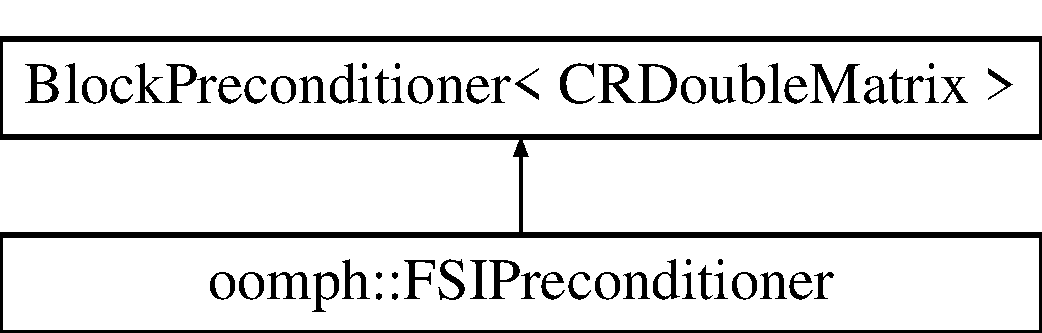
\includegraphics[height=2.000000cm]{classoomph_1_1FSIPreconditioner}
\end{center}
\end{figure}
\subsection*{Public Member Functions}
\begin{DoxyCompactItemize}
\item 
\hyperlink{classoomph_1_1FSIPreconditioner_aee06474cc9aabbde2dacb2cff1317a78}{F\+S\+I\+Preconditioner} (Problem $\ast$problem\+\_\+pt)
\begin{DoxyCompactList}\small\item\em Constructor\+: By default use block triangular form with retained fluid on solid terms. A problem pointer is required for the underlying Navier\+Stokes\+Schur\+Complement\+Preconditioner. \end{DoxyCompactList}\item 
\hyperlink{classoomph_1_1FSIPreconditioner_a787995de6ec09a9113b1b9a8b7c4f9cc}{$\sim$\+F\+S\+I\+Preconditioner} ()
\begin{DoxyCompactList}\small\item\em Destructor\+: Clean up. \end{DoxyCompactList}\item 
\hyperlink{classoomph_1_1FSIPreconditioner_a499de26b5f215957727155cf5f950019}{F\+S\+I\+Preconditioner} (const \hyperlink{classoomph_1_1FSIPreconditioner}{F\+S\+I\+Preconditioner} \&)
\begin{DoxyCompactList}\small\item\em Broken copy constructor. \end{DoxyCompactList}\item 
void \hyperlink{classoomph_1_1FSIPreconditioner_a0f21e38e18521e0946c3f3ec98a85baa}{set\+\_\+solid\+\_\+preconditioner\+\_\+pt} (Preconditioner $\ast$\hyperlink{classoomph_1_1FSIPreconditioner_abc97d84c4d0e7a280947855b7f33c34c}{solid\+\_\+preconditioner\+\_\+pt})
\begin{DoxyCompactList}\small\item\em Broken assignment operator. \end{DoxyCompactList}\item 
Preconditioner $\ast$ \hyperlink{classoomph_1_1FSIPreconditioner_abc97d84c4d0e7a280947855b7f33c34c}{solid\+\_\+preconditioner\+\_\+pt} () const
\begin{DoxyCompactList}\small\item\em Read-\/only access to solid preconditoner (use set\+\_\+... to set it) \end{DoxyCompactList}\item 
void \hyperlink{classoomph_1_1FSIPreconditioner_a8cdc0304cf22456a8b27ef95f5560e0b}{use\+\_\+block\+\_\+diagonal\+\_\+version} ()
\begin{DoxyCompactList}\small\item\em Switch to block-\/diagonal preconditioner. \end{DoxyCompactList}\item 
void \hyperlink{classoomph_1_1FSIPreconditioner_ad6e461da68c8e7f87b86f38fcd67ec69}{use\+\_\+block\+\_\+triangular\+\_\+version\+\_\+with\+\_\+fluid\+\_\+on\+\_\+solid} ()
\begin{DoxyCompactList}\small\item\em Switch to block-\/triangular preconditioner in which action of fluid dofs onto solid equations is retained. \end{DoxyCompactList}\item 
void \hyperlink{classoomph_1_1FSIPreconditioner_a193bbf986401ecb843e71581460004ad}{use\+\_\+block\+\_\+triangular\+\_\+version\+\_\+with\+\_\+solid\+\_\+on\+\_\+fluid} ()
\begin{DoxyCompactList}\small\item\em Switch to block-\/triangular preconditioner in which action of solid dofs onto fluid equations is retained. \end{DoxyCompactList}\item 
void \hyperlink{classoomph_1_1FSIPreconditioner_a5d70612246bd08bec6c7b373da5e9c80}{set\+\_\+navier\+\_\+stokes\+\_\+mesh} (Mesh $\ast$mesh\+\_\+pt, const bool \&allow\+\_\+multiple\+\_\+element\+\_\+type\+\_\+in\+\_\+navier\+\_\+stokes\+\_\+mesh=false)
\begin{DoxyCompactList}\small\item\em Setter function for the mesh containing the block-\/preconditionable Navier-\/\+Stokes elements. The optional argument indicates if there are more than one type of elements in same mesh. \end{DoxyCompactList}\item 
void \hyperlink{classoomph_1_1FSIPreconditioner_a61d583e9d3a1596efe22b11950fb47a5}{set\+\_\+wall\+\_\+mesh} (Mesh $\ast$mesh\+\_\+pt, const bool \&allow\+\_\+multiple\+\_\+element\+\_\+type\+\_\+in\+\_\+wall\+\_\+mesh=false)
\begin{DoxyCompactList}\small\item\em Setter function for the mesh containing the block-\/preconditionable F\+SI solid elements. The optional argument indicates if there are more than one type of elements in the same mesh. \end{DoxyCompactList}\item 
void \hyperlink{classoomph_1_1FSIPreconditioner_adadfe9f4332af610b00f1f45d1ad432e}{setup} ()
\begin{DoxyCompactList}\small\item\em Setup the preconditioner. \end{DoxyCompactList}\item 
void \hyperlink{classoomph_1_1FSIPreconditioner_a31c84c3ca19c31488acd0bf2fe333a6b}{preconditioner\+\_\+solve} (const Double\+Vector \&r, Double\+Vector \&z)
\begin{DoxyCompactList}\small\item\em Apply preconditioner to r. \end{DoxyCompactList}\item 
Navier\+Stokes\+Schur\+Complement\+Preconditioner $\ast$ \hyperlink{classoomph_1_1FSIPreconditioner_a8cd1be6bffd5014090350064177c0283}{navier\+\_\+stokes\+\_\+preconditioner\+\_\+pt} () const
\begin{DoxyCompactList}\small\item\em Access function to the Navier Stokes preconditioner (inexact solver) \end{DoxyCompactList}\item 
void \hyperlink{classoomph_1_1FSIPreconditioner_a2836b05d6eb81b807bd53b50dad7d3a0}{enable\+\_\+doc\+\_\+time} ()
\begin{DoxyCompactList}\small\item\em Enable documentation of time. \end{DoxyCompactList}\item 
void \hyperlink{classoomph_1_1FSIPreconditioner_a932cb1cf6a20503a5cbb43a6b67f2340}{disable\+\_\+doc\+\_\+time} ()
\begin{DoxyCompactList}\small\item\em Disable documentation of time. \end{DoxyCompactList}\end{DoxyCompactItemize}
\subsection*{Private Attributes}
\begin{DoxyCompactItemize}
\item 
Navier\+Stokes\+Schur\+Complement\+Preconditioner $\ast$ \hyperlink{classoomph_1_1FSIPreconditioner_adc98903b78d0bc97c40eb733eaf6e498}{Navier\+\_\+stokes\+\_\+preconditioner\+\_\+pt}
\begin{DoxyCompactList}\small\item\em Pointer the Navier Stokes preconditioner (inexact solver) \end{DoxyCompactList}\item 
Preconditioner $\ast$ \hyperlink{classoomph_1_1FSIPreconditioner_a9a6616d03bd67e2c1c406bcb6d332893}{Solid\+\_\+preconditioner\+\_\+pt}
\begin{DoxyCompactList}\small\item\em Pointer to the solid preconditioner (inexact solver) \end{DoxyCompactList}\item 
Matrix\+Vector\+Product $\ast$ \hyperlink{classoomph_1_1FSIPreconditioner_a595acfea83abd9fd907c208f3b487f57}{Matrix\+\_\+vector\+\_\+product\+\_\+0\+\_\+1\+\_\+pt}
\begin{DoxyCompactList}\small\item\em Pointer to fluid/solid interaction matrix. \end{DoxyCompactList}\item 
Matrix\+Vector\+Product $\ast$ \hyperlink{classoomph_1_1FSIPreconditioner_a8b4161c521cb4160ae07bb0096eaca1c}{Matrix\+\_\+vector\+\_\+product\+\_\+1\+\_\+0\+\_\+pt}
\begin{DoxyCompactList}\small\item\em Pointer to solid/fluid solid interaction matrix. \end{DoxyCompactList}\item 
bool \hyperlink{classoomph_1_1FSIPreconditioner_ad8d4b031c62a4ec74fad432a6bf27346}{Preconditioner\+\_\+has\+\_\+been\+\_\+setup}
\begin{DoxyCompactList}\small\item\em Boolean indicating the preconditioner has been set up. \end{DoxyCompactList}\item 
bool \hyperlink{classoomph_1_1FSIPreconditioner_acecba46494b0aa6f2035020f53be634c}{Retain\+\_\+solid\+\_\+onto\+\_\+fluid\+\_\+terms}
\begin{DoxyCompactList}\small\item\em Boolean flag used to indicate that the solid onto fluid interaction terms are to be retained. \end{DoxyCompactList}\item 
bool \hyperlink{classoomph_1_1FSIPreconditioner_ada9ff0aa8a1b15dea196a6d753ec740e}{Retain\+\_\+fluid\+\_\+onto\+\_\+solid\+\_\+terms}
\begin{DoxyCompactList}\small\item\em Boolean flag used to indicate that the fluid onto solid interaction terms are to be retained. \end{DoxyCompactList}\item 
bool \hyperlink{classoomph_1_1FSIPreconditioner_a405ccaf05553b1bf7702cb2f25df57e9}{Doc\+\_\+time}
\begin{DoxyCompactList}\small\item\em Set Doc\+\_\+time to true for outputting results of timings. \end{DoxyCompactList}\item 
Mesh $\ast$ \hyperlink{classoomph_1_1FSIPreconditioner_a201e3fcf3e13bd19b3871e9d3a734a1d}{Navier\+\_\+stokes\+\_\+mesh\+\_\+pt}
\begin{DoxyCompactList}\small\item\em Pointer to the navier stokes mesh. \end{DoxyCompactList}\item 
Mesh $\ast$ \hyperlink{classoomph_1_1FSIPreconditioner_ae86cf988796524f905c8d6edc942816a}{Wall\+\_\+mesh\+\_\+pt}
\begin{DoxyCompactList}\small\item\em pointer to the solid mesh \end{DoxyCompactList}\item 
bool \hyperlink{classoomph_1_1FSIPreconditioner_a4c015d18092bf2bfc1db075c74006e80}{Allow\+\_\+multiple\+\_\+element\+\_\+type\+\_\+in\+\_\+navier\+\_\+stokes\+\_\+mesh}
\item 
bool \hyperlink{classoomph_1_1FSIPreconditioner_a87e5a1cb279243414b1b0c2a5834efb5}{Allow\+\_\+multiple\+\_\+element\+\_\+type\+\_\+in\+\_\+wall\+\_\+mesh}
\end{DoxyCompactItemize}


\subsection{Detailed Description}
F\+SI preconditioner. This extracts upper/lower triangular blocks in the 3x3 overall block matrix structure arising from the monolithic discretisation of F\+SI problems with algebraic node updates. Dofs are decomposed into fluid velocity, pressure and solid unknowns. Navier\+Stokes\+Schur\+Complement\+Preconditioner is used as the inexact solver for the fluid block; Super\+LU (in its incarnation as an \char`\"{}exact\char`\"{} preconditioner) is used for the solid block. By default we retain the fluid on solid off diagonal blocks. 

Definition at line 58 of file fsi\+\_\+preconditioners.\+h.



\subsection{Constructor \& Destructor Documentation}
\mbox{\Hypertarget{classoomph_1_1FSIPreconditioner_aee06474cc9aabbde2dacb2cff1317a78}\label{classoomph_1_1FSIPreconditioner_aee06474cc9aabbde2dacb2cff1317a78}} 
\index{oomph\+::\+F\+S\+I\+Preconditioner@{oomph\+::\+F\+S\+I\+Preconditioner}!F\+S\+I\+Preconditioner@{F\+S\+I\+Preconditioner}}
\index{F\+S\+I\+Preconditioner@{F\+S\+I\+Preconditioner}!oomph\+::\+F\+S\+I\+Preconditioner@{oomph\+::\+F\+S\+I\+Preconditioner}}
\subsubsection{\texorpdfstring{F\+S\+I\+Preconditioner()}{FSIPreconditioner()}\hspace{0.1cm}{\footnotesize\ttfamily [1/2]}}
{\footnotesize\ttfamily oomph\+::\+F\+S\+I\+Preconditioner\+::\+F\+S\+I\+Preconditioner (\begin{DoxyParamCaption}\item[{Problem $\ast$}]{problem\+\_\+pt }\end{DoxyParamCaption})\hspace{0.3cm}{\ttfamily [inline]}}



Constructor\+: By default use block triangular form with retained fluid on solid terms. A problem pointer is required for the underlying Navier\+Stokes\+Schur\+Complement\+Preconditioner. 



Definition at line 66 of file fsi\+\_\+preconditioners.\+h.



References Allow\+\_\+multiple\+\_\+element\+\_\+type\+\_\+in\+\_\+navier\+\_\+stokes\+\_\+mesh, Allow\+\_\+multiple\+\_\+element\+\_\+type\+\_\+in\+\_\+wall\+\_\+mesh, Doc\+\_\+time, Matrix\+\_\+vector\+\_\+product\+\_\+0\+\_\+1\+\_\+pt, Matrix\+\_\+vector\+\_\+product\+\_\+1\+\_\+0\+\_\+pt, Navier\+\_\+stokes\+\_\+mesh\+\_\+pt, Navier\+\_\+stokes\+\_\+preconditioner\+\_\+pt, Preconditioner\+\_\+has\+\_\+been\+\_\+setup, Retain\+\_\+fluid\+\_\+onto\+\_\+solid\+\_\+terms, Retain\+\_\+solid\+\_\+onto\+\_\+fluid\+\_\+terms, Solid\+\_\+preconditioner\+\_\+pt, and Wall\+\_\+mesh\+\_\+pt.

\mbox{\Hypertarget{classoomph_1_1FSIPreconditioner_a787995de6ec09a9113b1b9a8b7c4f9cc}\label{classoomph_1_1FSIPreconditioner_a787995de6ec09a9113b1b9a8b7c4f9cc}} 
\index{oomph\+::\+F\+S\+I\+Preconditioner@{oomph\+::\+F\+S\+I\+Preconditioner}!````~F\+S\+I\+Preconditioner@{$\sim$\+F\+S\+I\+Preconditioner}}
\index{````~F\+S\+I\+Preconditioner@{$\sim$\+F\+S\+I\+Preconditioner}!oomph\+::\+F\+S\+I\+Preconditioner@{oomph\+::\+F\+S\+I\+Preconditioner}}
\subsubsection{\texorpdfstring{$\sim$\+F\+S\+I\+Preconditioner()}{~FSIPreconditioner()}}
{\footnotesize\ttfamily oomph\+::\+F\+S\+I\+Preconditioner\+::$\sim$\+F\+S\+I\+Preconditioner (\begin{DoxyParamCaption}{ }\end{DoxyParamCaption})\hspace{0.3cm}{\ttfamily [inline]}}



Destructor\+: Clean up. 



Definition at line 102 of file fsi\+\_\+preconditioners.\+h.



References Matrix\+\_\+vector\+\_\+product\+\_\+0\+\_\+1\+\_\+pt, Matrix\+\_\+vector\+\_\+product\+\_\+1\+\_\+0\+\_\+pt, Navier\+\_\+stokes\+\_\+preconditioner\+\_\+pt, and Solid\+\_\+preconditioner\+\_\+pt.

\mbox{\Hypertarget{classoomph_1_1FSIPreconditioner_a499de26b5f215957727155cf5f950019}\label{classoomph_1_1FSIPreconditioner_a499de26b5f215957727155cf5f950019}} 
\index{oomph\+::\+F\+S\+I\+Preconditioner@{oomph\+::\+F\+S\+I\+Preconditioner}!F\+S\+I\+Preconditioner@{F\+S\+I\+Preconditioner}}
\index{F\+S\+I\+Preconditioner@{F\+S\+I\+Preconditioner}!oomph\+::\+F\+S\+I\+Preconditioner@{oomph\+::\+F\+S\+I\+Preconditioner}}
\subsubsection{\texorpdfstring{F\+S\+I\+Preconditioner()}{FSIPreconditioner()}\hspace{0.1cm}{\footnotesize\ttfamily [2/2]}}
{\footnotesize\ttfamily oomph\+::\+F\+S\+I\+Preconditioner\+::\+F\+S\+I\+Preconditioner (\begin{DoxyParamCaption}\item[{const \hyperlink{classoomph_1_1FSIPreconditioner}{F\+S\+I\+Preconditioner} \&}]{ }\end{DoxyParamCaption})\hspace{0.3cm}{\ttfamily [inline]}}



Broken copy constructor. 



Definition at line 117 of file fsi\+\_\+preconditioners.\+h.



\subsection{Member Function Documentation}
\mbox{\Hypertarget{classoomph_1_1FSIPreconditioner_a932cb1cf6a20503a5cbb43a6b67f2340}\label{classoomph_1_1FSIPreconditioner_a932cb1cf6a20503a5cbb43a6b67f2340}} 
\index{oomph\+::\+F\+S\+I\+Preconditioner@{oomph\+::\+F\+S\+I\+Preconditioner}!disable\+\_\+doc\+\_\+time@{disable\+\_\+doc\+\_\+time}}
\index{disable\+\_\+doc\+\_\+time@{disable\+\_\+doc\+\_\+time}!oomph\+::\+F\+S\+I\+Preconditioner@{oomph\+::\+F\+S\+I\+Preconditioner}}
\subsubsection{\texorpdfstring{disable\+\_\+doc\+\_\+time()}{disable\_doc\_time()}}
{\footnotesize\ttfamily void oomph\+::\+F\+S\+I\+Preconditioner\+::disable\+\_\+doc\+\_\+time (\begin{DoxyParamCaption}{ }\end{DoxyParamCaption})\hspace{0.3cm}{\ttfamily [inline]}}



Disable documentation of time. 



Definition at line 221 of file fsi\+\_\+preconditioners.\+h.



References Doc\+\_\+time.

\mbox{\Hypertarget{classoomph_1_1FSIPreconditioner_a2836b05d6eb81b807bd53b50dad7d3a0}\label{classoomph_1_1FSIPreconditioner_a2836b05d6eb81b807bd53b50dad7d3a0}} 
\index{oomph\+::\+F\+S\+I\+Preconditioner@{oomph\+::\+F\+S\+I\+Preconditioner}!enable\+\_\+doc\+\_\+time@{enable\+\_\+doc\+\_\+time}}
\index{enable\+\_\+doc\+\_\+time@{enable\+\_\+doc\+\_\+time}!oomph\+::\+F\+S\+I\+Preconditioner@{oomph\+::\+F\+S\+I\+Preconditioner}}
\subsubsection{\texorpdfstring{enable\+\_\+doc\+\_\+time()}{enable\_doc\_time()}}
{\footnotesize\ttfamily void oomph\+::\+F\+S\+I\+Preconditioner\+::enable\+\_\+doc\+\_\+time (\begin{DoxyParamCaption}{ }\end{DoxyParamCaption})\hspace{0.3cm}{\ttfamily [inline]}}



Enable documentation of time. 



Definition at line 218 of file fsi\+\_\+preconditioners.\+h.



References Doc\+\_\+time.

\mbox{\Hypertarget{classoomph_1_1FSIPreconditioner_a8cd1be6bffd5014090350064177c0283}\label{classoomph_1_1FSIPreconditioner_a8cd1be6bffd5014090350064177c0283}} 
\index{oomph\+::\+F\+S\+I\+Preconditioner@{oomph\+::\+F\+S\+I\+Preconditioner}!navier\+\_\+stokes\+\_\+preconditioner\+\_\+pt@{navier\+\_\+stokes\+\_\+preconditioner\+\_\+pt}}
\index{navier\+\_\+stokes\+\_\+preconditioner\+\_\+pt@{navier\+\_\+stokes\+\_\+preconditioner\+\_\+pt}!oomph\+::\+F\+S\+I\+Preconditioner@{oomph\+::\+F\+S\+I\+Preconditioner}}
\subsubsection{\texorpdfstring{navier\+\_\+stokes\+\_\+preconditioner\+\_\+pt()}{navier\_stokes\_preconditioner\_pt()}}
{\footnotesize\ttfamily Navier\+Stokes\+Schur\+Complement\+Preconditioner$\ast$ oomph\+::\+F\+S\+I\+Preconditioner\+::navier\+\_\+stokes\+\_\+preconditioner\+\_\+pt (\begin{DoxyParamCaption}{ }\end{DoxyParamCaption}) const\hspace{0.3cm}{\ttfamily [inline]}}



Access function to the Navier Stokes preconditioner (inexact solver) 



Definition at line 212 of file fsi\+\_\+preconditioners.\+h.



References Navier\+\_\+stokes\+\_\+preconditioner\+\_\+pt.

\mbox{\Hypertarget{classoomph_1_1FSIPreconditioner_a31c84c3ca19c31488acd0bf2fe333a6b}\label{classoomph_1_1FSIPreconditioner_a31c84c3ca19c31488acd0bf2fe333a6b}} 
\index{oomph\+::\+F\+S\+I\+Preconditioner@{oomph\+::\+F\+S\+I\+Preconditioner}!preconditioner\+\_\+solve@{preconditioner\+\_\+solve}}
\index{preconditioner\+\_\+solve@{preconditioner\+\_\+solve}!oomph\+::\+F\+S\+I\+Preconditioner@{oomph\+::\+F\+S\+I\+Preconditioner}}
\subsubsection{\texorpdfstring{preconditioner\+\_\+solve()}{preconditioner\_solve()}}
{\footnotesize\ttfamily void oomph\+::\+F\+S\+I\+Preconditioner\+::preconditioner\+\_\+solve (\begin{DoxyParamCaption}\item[{const Double\+Vector \&}]{r,  }\item[{Double\+Vector \&}]{z }\end{DoxyParamCaption})}



Apply preconditioner to r. 

Apply preconditioner to Vector r. 

Definition at line 385 of file fsi\+\_\+preconditioners.\+h.



References Matrix\+\_\+vector\+\_\+product\+\_\+0\+\_\+1\+\_\+pt, Matrix\+\_\+vector\+\_\+product\+\_\+1\+\_\+0\+\_\+pt, Navier\+\_\+stokes\+\_\+preconditioner\+\_\+pt, Retain\+\_\+fluid\+\_\+onto\+\_\+solid\+\_\+terms, Retain\+\_\+solid\+\_\+onto\+\_\+fluid\+\_\+terms, and Solid\+\_\+preconditioner\+\_\+pt.



Referenced by set\+\_\+wall\+\_\+mesh(), and oomph\+::\+Simple\+F\+S\+I\+Preconditioner$<$ M\+A\+T\+R\+I\+X $>$\+::set\+\_\+wall\+\_\+mesh().

\mbox{\Hypertarget{classoomph_1_1FSIPreconditioner_a5d70612246bd08bec6c7b373da5e9c80}\label{classoomph_1_1FSIPreconditioner_a5d70612246bd08bec6c7b373da5e9c80}} 
\index{oomph\+::\+F\+S\+I\+Preconditioner@{oomph\+::\+F\+S\+I\+Preconditioner}!set\+\_\+navier\+\_\+stokes\+\_\+mesh@{set\+\_\+navier\+\_\+stokes\+\_\+mesh}}
\index{set\+\_\+navier\+\_\+stokes\+\_\+mesh@{set\+\_\+navier\+\_\+stokes\+\_\+mesh}!oomph\+::\+F\+S\+I\+Preconditioner@{oomph\+::\+F\+S\+I\+Preconditioner}}
\subsubsection{\texorpdfstring{set\+\_\+navier\+\_\+stokes\+\_\+mesh()}{set\_navier\_stokes\_mesh()}}
{\footnotesize\ttfamily void oomph\+::\+F\+S\+I\+Preconditioner\+::set\+\_\+navier\+\_\+stokes\+\_\+mesh (\begin{DoxyParamCaption}\item[{Mesh $\ast$}]{mesh\+\_\+pt,  }\item[{const bool \&}]{allow\+\_\+multiple\+\_\+element\+\_\+type\+\_\+in\+\_\+navier\+\_\+stokes\+\_\+mesh = {\ttfamily false} }\end{DoxyParamCaption})\hspace{0.3cm}{\ttfamily [inline]}}



Setter function for the mesh containing the block-\/preconditionable Navier-\/\+Stokes elements. The optional argument indicates if there are more than one type of elements in same mesh. 



Definition at line 178 of file fsi\+\_\+preconditioners.\+h.



References Allow\+\_\+multiple\+\_\+element\+\_\+type\+\_\+in\+\_\+navier\+\_\+stokes\+\_\+mesh, and Navier\+\_\+stokes\+\_\+mesh\+\_\+pt.



Referenced by setup(), oomph\+::\+Simple\+F\+S\+I\+Preconditioner$<$ M\+A\+T\+R\+I\+X $>$\+::\+Simple\+F\+S\+I\+Preconditioner(), and use\+\_\+block\+\_\+triangular\+\_\+version\+\_\+with\+\_\+solid\+\_\+on\+\_\+fluid().

\mbox{\Hypertarget{classoomph_1_1FSIPreconditioner_a0f21e38e18521e0946c3f3ec98a85baa}\label{classoomph_1_1FSIPreconditioner_a0f21e38e18521e0946c3f3ec98a85baa}} 
\index{oomph\+::\+F\+S\+I\+Preconditioner@{oomph\+::\+F\+S\+I\+Preconditioner}!set\+\_\+solid\+\_\+preconditioner\+\_\+pt@{set\+\_\+solid\+\_\+preconditioner\+\_\+pt}}
\index{set\+\_\+solid\+\_\+preconditioner\+\_\+pt@{set\+\_\+solid\+\_\+preconditioner\+\_\+pt}!oomph\+::\+F\+S\+I\+Preconditioner@{oomph\+::\+F\+S\+I\+Preconditioner}}
\subsubsection{\texorpdfstring{set\+\_\+solid\+\_\+preconditioner\+\_\+pt()}{set\_solid\_preconditioner\_pt()}}
{\footnotesize\ttfamily void oomph\+::\+F\+S\+I\+Preconditioner\+::set\+\_\+solid\+\_\+preconditioner\+\_\+pt (\begin{DoxyParamCaption}\item[{Preconditioner $\ast$}]{solid\+\_\+preconditioner\+\_\+pt }\end{DoxyParamCaption})\hspace{0.3cm}{\ttfamily [inline]}}



Broken assignment operator. 

Set solid preconditioner (deletes existing one) 

Definition at line 134 of file fsi\+\_\+preconditioners.\+h.



References solid\+\_\+preconditioner\+\_\+pt(), and Solid\+\_\+preconditioner\+\_\+pt.

\mbox{\Hypertarget{classoomph_1_1FSIPreconditioner_a61d583e9d3a1596efe22b11950fb47a5}\label{classoomph_1_1FSIPreconditioner_a61d583e9d3a1596efe22b11950fb47a5}} 
\index{oomph\+::\+F\+S\+I\+Preconditioner@{oomph\+::\+F\+S\+I\+Preconditioner}!set\+\_\+wall\+\_\+mesh@{set\+\_\+wall\+\_\+mesh}}
\index{set\+\_\+wall\+\_\+mesh@{set\+\_\+wall\+\_\+mesh}!oomph\+::\+F\+S\+I\+Preconditioner@{oomph\+::\+F\+S\+I\+Preconditioner}}
\subsubsection{\texorpdfstring{set\+\_\+wall\+\_\+mesh()}{set\_wall\_mesh()}}
{\footnotesize\ttfamily void oomph\+::\+F\+S\+I\+Preconditioner\+::set\+\_\+wall\+\_\+mesh (\begin{DoxyParamCaption}\item[{Mesh $\ast$}]{mesh\+\_\+pt,  }\item[{const bool \&}]{allow\+\_\+multiple\+\_\+element\+\_\+type\+\_\+in\+\_\+wall\+\_\+mesh = {\ttfamily false} }\end{DoxyParamCaption})\hspace{0.3cm}{\ttfamily [inline]}}



Setter function for the mesh containing the block-\/preconditionable F\+SI solid elements. The optional argument indicates if there are more than one type of elements in the same mesh. 



Definition at line 192 of file fsi\+\_\+preconditioners.\+h.



References Allow\+\_\+multiple\+\_\+element\+\_\+type\+\_\+in\+\_\+wall\+\_\+mesh, preconditioner\+\_\+solve(), setup(), and Wall\+\_\+mesh\+\_\+pt.



Referenced by oomph\+::\+Simple\+F\+S\+I\+Preconditioner$<$ M\+A\+T\+R\+I\+X $>$\+::set\+\_\+navier\+\_\+stokes\+\_\+mesh().

\mbox{\Hypertarget{classoomph_1_1FSIPreconditioner_adadfe9f4332af610b00f1f45d1ad432e}\label{classoomph_1_1FSIPreconditioner_adadfe9f4332af610b00f1f45d1ad432e}} 
\index{oomph\+::\+F\+S\+I\+Preconditioner@{oomph\+::\+F\+S\+I\+Preconditioner}!setup@{setup}}
\index{setup@{setup}!oomph\+::\+F\+S\+I\+Preconditioner@{oomph\+::\+F\+S\+I\+Preconditioner}}
\subsubsection{\texorpdfstring{setup()}{setup()}}
{\footnotesize\ttfamily void oomph\+::\+F\+S\+I\+Preconditioner\+::setup (\begin{DoxyParamCaption}{ }\end{DoxyParamCaption})}



Setup the preconditioner. 

Setup the preconditioner. Note\+: Matrix must be a C\+R\+Double\+Matrix. 

Definition at line 279 of file fsi\+\_\+preconditioners.\+h.



References Allow\+\_\+multiple\+\_\+element\+\_\+type\+\_\+in\+\_\+navier\+\_\+stokes\+\_\+mesh, Allow\+\_\+multiple\+\_\+element\+\_\+type\+\_\+in\+\_\+wall\+\_\+mesh, Doc\+\_\+time, Matrix\+\_\+vector\+\_\+product\+\_\+0\+\_\+1\+\_\+pt, Matrix\+\_\+vector\+\_\+product\+\_\+1\+\_\+0\+\_\+pt, Navier\+\_\+stokes\+\_\+mesh\+\_\+pt, Navier\+\_\+stokes\+\_\+preconditioner\+\_\+pt, Preconditioner\+\_\+has\+\_\+been\+\_\+setup, Retain\+\_\+fluid\+\_\+onto\+\_\+solid\+\_\+terms, Retain\+\_\+solid\+\_\+onto\+\_\+fluid\+\_\+terms, set\+\_\+navier\+\_\+stokes\+\_\+mesh(), Solid\+\_\+preconditioner\+\_\+pt, and Wall\+\_\+mesh\+\_\+pt.



Referenced by set\+\_\+wall\+\_\+mesh(), and oomph\+::\+Simple\+F\+S\+I\+Preconditioner$<$ M\+A\+T\+R\+I\+X $>$\+::set\+\_\+wall\+\_\+mesh().

\mbox{\Hypertarget{classoomph_1_1FSIPreconditioner_abc97d84c4d0e7a280947855b7f33c34c}\label{classoomph_1_1FSIPreconditioner_abc97d84c4d0e7a280947855b7f33c34c}} 
\index{oomph\+::\+F\+S\+I\+Preconditioner@{oomph\+::\+F\+S\+I\+Preconditioner}!solid\+\_\+preconditioner\+\_\+pt@{solid\+\_\+preconditioner\+\_\+pt}}
\index{solid\+\_\+preconditioner\+\_\+pt@{solid\+\_\+preconditioner\+\_\+pt}!oomph\+::\+F\+S\+I\+Preconditioner@{oomph\+::\+F\+S\+I\+Preconditioner}}
\subsubsection{\texorpdfstring{solid\+\_\+preconditioner\+\_\+pt()}{solid\_preconditioner\_pt()}}
{\footnotesize\ttfamily Preconditioner$\ast$ oomph\+::\+F\+S\+I\+Preconditioner\+::solid\+\_\+preconditioner\+\_\+pt (\begin{DoxyParamCaption}{ }\end{DoxyParamCaption}) const\hspace{0.3cm}{\ttfamily [inline]}}



Read-\/only access to solid preconditoner (use set\+\_\+... to set it) 



Definition at line 145 of file fsi\+\_\+preconditioners.\+h.



References Solid\+\_\+preconditioner\+\_\+pt.



Referenced by set\+\_\+solid\+\_\+preconditioner\+\_\+pt().

\mbox{\Hypertarget{classoomph_1_1FSIPreconditioner_a8cdc0304cf22456a8b27ef95f5560e0b}\label{classoomph_1_1FSIPreconditioner_a8cdc0304cf22456a8b27ef95f5560e0b}} 
\index{oomph\+::\+F\+S\+I\+Preconditioner@{oomph\+::\+F\+S\+I\+Preconditioner}!use\+\_\+block\+\_\+diagonal\+\_\+version@{use\+\_\+block\+\_\+diagonal\+\_\+version}}
\index{use\+\_\+block\+\_\+diagonal\+\_\+version@{use\+\_\+block\+\_\+diagonal\+\_\+version}!oomph\+::\+F\+S\+I\+Preconditioner@{oomph\+::\+F\+S\+I\+Preconditioner}}
\subsubsection{\texorpdfstring{use\+\_\+block\+\_\+diagonal\+\_\+version()}{use\_block\_diagonal\_version()}}
{\footnotesize\ttfamily void oomph\+::\+F\+S\+I\+Preconditioner\+::use\+\_\+block\+\_\+diagonal\+\_\+version (\begin{DoxyParamCaption}{ }\end{DoxyParamCaption})\hspace{0.3cm}{\ttfamily [inline]}}



Switch to block-\/diagonal preconditioner. 



Definition at line 152 of file fsi\+\_\+preconditioners.\+h.



References Retain\+\_\+fluid\+\_\+onto\+\_\+solid\+\_\+terms, and Retain\+\_\+solid\+\_\+onto\+\_\+fluid\+\_\+terms.

\mbox{\Hypertarget{classoomph_1_1FSIPreconditioner_ad6e461da68c8e7f87b86f38fcd67ec69}\label{classoomph_1_1FSIPreconditioner_ad6e461da68c8e7f87b86f38fcd67ec69}} 
\index{oomph\+::\+F\+S\+I\+Preconditioner@{oomph\+::\+F\+S\+I\+Preconditioner}!use\+\_\+block\+\_\+triangular\+\_\+version\+\_\+with\+\_\+fluid\+\_\+on\+\_\+solid@{use\+\_\+block\+\_\+triangular\+\_\+version\+\_\+with\+\_\+fluid\+\_\+on\+\_\+solid}}
\index{use\+\_\+block\+\_\+triangular\+\_\+version\+\_\+with\+\_\+fluid\+\_\+on\+\_\+solid@{use\+\_\+block\+\_\+triangular\+\_\+version\+\_\+with\+\_\+fluid\+\_\+on\+\_\+solid}!oomph\+::\+F\+S\+I\+Preconditioner@{oomph\+::\+F\+S\+I\+Preconditioner}}
\subsubsection{\texorpdfstring{use\+\_\+block\+\_\+triangular\+\_\+version\+\_\+with\+\_\+fluid\+\_\+on\+\_\+solid()}{use\_block\_triangular\_version\_with\_fluid\_on\_solid()}}
{\footnotesize\ttfamily void oomph\+::\+F\+S\+I\+Preconditioner\+::use\+\_\+block\+\_\+triangular\+\_\+version\+\_\+with\+\_\+fluid\+\_\+on\+\_\+solid (\begin{DoxyParamCaption}{ }\end{DoxyParamCaption})\hspace{0.3cm}{\ttfamily [inline]}}



Switch to block-\/triangular preconditioner in which action of fluid dofs onto solid equations is retained. 



Definition at line 160 of file fsi\+\_\+preconditioners.\+h.



References Retain\+\_\+fluid\+\_\+onto\+\_\+solid\+\_\+terms, and Retain\+\_\+solid\+\_\+onto\+\_\+fluid\+\_\+terms.

\mbox{\Hypertarget{classoomph_1_1FSIPreconditioner_a193bbf986401ecb843e71581460004ad}\label{classoomph_1_1FSIPreconditioner_a193bbf986401ecb843e71581460004ad}} 
\index{oomph\+::\+F\+S\+I\+Preconditioner@{oomph\+::\+F\+S\+I\+Preconditioner}!use\+\_\+block\+\_\+triangular\+\_\+version\+\_\+with\+\_\+solid\+\_\+on\+\_\+fluid@{use\+\_\+block\+\_\+triangular\+\_\+version\+\_\+with\+\_\+solid\+\_\+on\+\_\+fluid}}
\index{use\+\_\+block\+\_\+triangular\+\_\+version\+\_\+with\+\_\+solid\+\_\+on\+\_\+fluid@{use\+\_\+block\+\_\+triangular\+\_\+version\+\_\+with\+\_\+solid\+\_\+on\+\_\+fluid}!oomph\+::\+F\+S\+I\+Preconditioner@{oomph\+::\+F\+S\+I\+Preconditioner}}
\subsubsection{\texorpdfstring{use\+\_\+block\+\_\+triangular\+\_\+version\+\_\+with\+\_\+solid\+\_\+on\+\_\+fluid()}{use\_block\_triangular\_version\_with\_solid\_on\_fluid()}}
{\footnotesize\ttfamily void oomph\+::\+F\+S\+I\+Preconditioner\+::use\+\_\+block\+\_\+triangular\+\_\+version\+\_\+with\+\_\+solid\+\_\+on\+\_\+fluid (\begin{DoxyParamCaption}{ }\end{DoxyParamCaption})\hspace{0.3cm}{\ttfamily [inline]}}



Switch to block-\/triangular preconditioner in which action of solid dofs onto fluid equations is retained. 



Definition at line 168 of file fsi\+\_\+preconditioners.\+h.



References Retain\+\_\+fluid\+\_\+onto\+\_\+solid\+\_\+terms, Retain\+\_\+solid\+\_\+onto\+\_\+fluid\+\_\+terms, and set\+\_\+navier\+\_\+stokes\+\_\+mesh().



\subsection{Member Data Documentation}
\mbox{\Hypertarget{classoomph_1_1FSIPreconditioner_a4c015d18092bf2bfc1db075c74006e80}\label{classoomph_1_1FSIPreconditioner_a4c015d18092bf2bfc1db075c74006e80}} 
\index{oomph\+::\+F\+S\+I\+Preconditioner@{oomph\+::\+F\+S\+I\+Preconditioner}!Allow\+\_\+multiple\+\_\+element\+\_\+type\+\_\+in\+\_\+navier\+\_\+stokes\+\_\+mesh@{Allow\+\_\+multiple\+\_\+element\+\_\+type\+\_\+in\+\_\+navier\+\_\+stokes\+\_\+mesh}}
\index{Allow\+\_\+multiple\+\_\+element\+\_\+type\+\_\+in\+\_\+navier\+\_\+stokes\+\_\+mesh@{Allow\+\_\+multiple\+\_\+element\+\_\+type\+\_\+in\+\_\+navier\+\_\+stokes\+\_\+mesh}!oomph\+::\+F\+S\+I\+Preconditioner@{oomph\+::\+F\+S\+I\+Preconditioner}}
\subsubsection{\texorpdfstring{Allow\+\_\+multiple\+\_\+element\+\_\+type\+\_\+in\+\_\+navier\+\_\+stokes\+\_\+mesh}{Allow\_multiple\_element\_type\_in\_navier\_stokes\_mesh}}
{\footnotesize\ttfamily bool oomph\+::\+F\+S\+I\+Preconditioner\+::\+Allow\+\_\+multiple\+\_\+element\+\_\+type\+\_\+in\+\_\+navier\+\_\+stokes\+\_\+mesh\hspace{0.3cm}{\ttfamily [private]}}

Flag to indicate if there are multiple element types in the Navier-\/\+Stokes mesh. 

Definition at line 260 of file fsi\+\_\+preconditioners.\+h.



Referenced by F\+S\+I\+Preconditioner(), set\+\_\+navier\+\_\+stokes\+\_\+mesh(), oomph\+::\+Simple\+F\+S\+I\+Preconditioner$<$ M\+A\+T\+R\+I\+X $>$\+::set\+\_\+navier\+\_\+stokes\+\_\+mesh(), setup(), oomph\+::\+Simple\+F\+S\+I\+Preconditioner$<$ M\+A\+T\+R\+I\+X $>$\+::setup(), and oomph\+::\+Simple\+F\+S\+I\+Preconditioner$<$ M\+A\+T\+R\+I\+X $>$\+::\+Simple\+F\+S\+I\+Preconditioner().

\mbox{\Hypertarget{classoomph_1_1FSIPreconditioner_a87e5a1cb279243414b1b0c2a5834efb5}\label{classoomph_1_1FSIPreconditioner_a87e5a1cb279243414b1b0c2a5834efb5}} 
\index{oomph\+::\+F\+S\+I\+Preconditioner@{oomph\+::\+F\+S\+I\+Preconditioner}!Allow\+\_\+multiple\+\_\+element\+\_\+type\+\_\+in\+\_\+wall\+\_\+mesh@{Allow\+\_\+multiple\+\_\+element\+\_\+type\+\_\+in\+\_\+wall\+\_\+mesh}}
\index{Allow\+\_\+multiple\+\_\+element\+\_\+type\+\_\+in\+\_\+wall\+\_\+mesh@{Allow\+\_\+multiple\+\_\+element\+\_\+type\+\_\+in\+\_\+wall\+\_\+mesh}!oomph\+::\+F\+S\+I\+Preconditioner@{oomph\+::\+F\+S\+I\+Preconditioner}}
\subsubsection{\texorpdfstring{Allow\+\_\+multiple\+\_\+element\+\_\+type\+\_\+in\+\_\+wall\+\_\+mesh}{Allow\_multiple\_element\_type\_in\_wall\_mesh}}
{\footnotesize\ttfamily bool oomph\+::\+F\+S\+I\+Preconditioner\+::\+Allow\+\_\+multiple\+\_\+element\+\_\+type\+\_\+in\+\_\+wall\+\_\+mesh\hspace{0.3cm}{\ttfamily [private]}}



Definition at line 263 of file fsi\+\_\+preconditioners.\+h.



Referenced by F\+S\+I\+Preconditioner(), set\+\_\+wall\+\_\+mesh(), oomph\+::\+Simple\+F\+S\+I\+Preconditioner$<$ M\+A\+T\+R\+I\+X $>$\+::set\+\_\+wall\+\_\+mesh(), setup(), oomph\+::\+Simple\+F\+S\+I\+Preconditioner$<$ M\+A\+T\+R\+I\+X $>$\+::setup(), and oomph\+::\+Simple\+F\+S\+I\+Preconditioner$<$ M\+A\+T\+R\+I\+X $>$\+::\+Simple\+F\+S\+I\+Preconditioner().

\mbox{\Hypertarget{classoomph_1_1FSIPreconditioner_a405ccaf05553b1bf7702cb2f25df57e9}\label{classoomph_1_1FSIPreconditioner_a405ccaf05553b1bf7702cb2f25df57e9}} 
\index{oomph\+::\+F\+S\+I\+Preconditioner@{oomph\+::\+F\+S\+I\+Preconditioner}!Doc\+\_\+time@{Doc\+\_\+time}}
\index{Doc\+\_\+time@{Doc\+\_\+time}!oomph\+::\+F\+S\+I\+Preconditioner@{oomph\+::\+F\+S\+I\+Preconditioner}}
\subsubsection{\texorpdfstring{Doc\+\_\+time}{Doc\_time}}
{\footnotesize\ttfamily bool oomph\+::\+F\+S\+I\+Preconditioner\+::\+Doc\+\_\+time\hspace{0.3cm}{\ttfamily [private]}}



Set Doc\+\_\+time to true for outputting results of timings. 



Definition at line 250 of file fsi\+\_\+preconditioners.\+h.



Referenced by disable\+\_\+doc\+\_\+time(), enable\+\_\+doc\+\_\+time(), F\+S\+I\+Preconditioner(), and setup().

\mbox{\Hypertarget{classoomph_1_1FSIPreconditioner_a595acfea83abd9fd907c208f3b487f57}\label{classoomph_1_1FSIPreconditioner_a595acfea83abd9fd907c208f3b487f57}} 
\index{oomph\+::\+F\+S\+I\+Preconditioner@{oomph\+::\+F\+S\+I\+Preconditioner}!Matrix\+\_\+vector\+\_\+product\+\_\+0\+\_\+1\+\_\+pt@{Matrix\+\_\+vector\+\_\+product\+\_\+0\+\_\+1\+\_\+pt}}
\index{Matrix\+\_\+vector\+\_\+product\+\_\+0\+\_\+1\+\_\+pt@{Matrix\+\_\+vector\+\_\+product\+\_\+0\+\_\+1\+\_\+pt}!oomph\+::\+F\+S\+I\+Preconditioner@{oomph\+::\+F\+S\+I\+Preconditioner}}
\subsubsection{\texorpdfstring{Matrix\+\_\+vector\+\_\+product\+\_\+0\+\_\+1\+\_\+pt}{Matrix\_vector\_product\_0\_1\_pt}}
{\footnotesize\ttfamily Matrix\+Vector\+Product$\ast$ oomph\+::\+F\+S\+I\+Preconditioner\+::\+Matrix\+\_\+vector\+\_\+product\+\_\+0\+\_\+1\+\_\+pt\hspace{0.3cm}{\ttfamily [private]}}



Pointer to fluid/solid interaction matrix. 



Definition at line 233 of file fsi\+\_\+preconditioners.\+h.



Referenced by F\+S\+I\+Preconditioner(), preconditioner\+\_\+solve(), setup(), and $\sim$\+F\+S\+I\+Preconditioner().

\mbox{\Hypertarget{classoomph_1_1FSIPreconditioner_a8b4161c521cb4160ae07bb0096eaca1c}\label{classoomph_1_1FSIPreconditioner_a8b4161c521cb4160ae07bb0096eaca1c}} 
\index{oomph\+::\+F\+S\+I\+Preconditioner@{oomph\+::\+F\+S\+I\+Preconditioner}!Matrix\+\_\+vector\+\_\+product\+\_\+1\+\_\+0\+\_\+pt@{Matrix\+\_\+vector\+\_\+product\+\_\+1\+\_\+0\+\_\+pt}}
\index{Matrix\+\_\+vector\+\_\+product\+\_\+1\+\_\+0\+\_\+pt@{Matrix\+\_\+vector\+\_\+product\+\_\+1\+\_\+0\+\_\+pt}!oomph\+::\+F\+S\+I\+Preconditioner@{oomph\+::\+F\+S\+I\+Preconditioner}}
\subsubsection{\texorpdfstring{Matrix\+\_\+vector\+\_\+product\+\_\+1\+\_\+0\+\_\+pt}{Matrix\_vector\_product\_1\_0\_pt}}
{\footnotesize\ttfamily Matrix\+Vector\+Product$\ast$ oomph\+::\+F\+S\+I\+Preconditioner\+::\+Matrix\+\_\+vector\+\_\+product\+\_\+1\+\_\+0\+\_\+pt\hspace{0.3cm}{\ttfamily [private]}}



Pointer to solid/fluid solid interaction matrix. 



Definition at line 236 of file fsi\+\_\+preconditioners.\+h.



Referenced by F\+S\+I\+Preconditioner(), preconditioner\+\_\+solve(), setup(), and $\sim$\+F\+S\+I\+Preconditioner().

\mbox{\Hypertarget{classoomph_1_1FSIPreconditioner_a201e3fcf3e13bd19b3871e9d3a734a1d}\label{classoomph_1_1FSIPreconditioner_a201e3fcf3e13bd19b3871e9d3a734a1d}} 
\index{oomph\+::\+F\+S\+I\+Preconditioner@{oomph\+::\+F\+S\+I\+Preconditioner}!Navier\+\_\+stokes\+\_\+mesh\+\_\+pt@{Navier\+\_\+stokes\+\_\+mesh\+\_\+pt}}
\index{Navier\+\_\+stokes\+\_\+mesh\+\_\+pt@{Navier\+\_\+stokes\+\_\+mesh\+\_\+pt}!oomph\+::\+F\+S\+I\+Preconditioner@{oomph\+::\+F\+S\+I\+Preconditioner}}
\subsubsection{\texorpdfstring{Navier\+\_\+stokes\+\_\+mesh\+\_\+pt}{Navier\_stokes\_mesh\_pt}}
{\footnotesize\ttfamily Mesh$\ast$ oomph\+::\+F\+S\+I\+Preconditioner\+::\+Navier\+\_\+stokes\+\_\+mesh\+\_\+pt\hspace{0.3cm}{\ttfamily [private]}}



Pointer to the navier stokes mesh. 



Definition at line 253 of file fsi\+\_\+preconditioners.\+h.



Referenced by F\+S\+I\+Preconditioner(), set\+\_\+navier\+\_\+stokes\+\_\+mesh(), oomph\+::\+Simple\+F\+S\+I\+Preconditioner$<$ M\+A\+T\+R\+I\+X $>$\+::set\+\_\+navier\+\_\+stokes\+\_\+mesh(), setup(), oomph\+::\+Simple\+F\+S\+I\+Preconditioner$<$ M\+A\+T\+R\+I\+X $>$\+::setup(), and oomph\+::\+Simple\+F\+S\+I\+Preconditioner$<$ M\+A\+T\+R\+I\+X $>$\+::\+Simple\+F\+S\+I\+Preconditioner().

\mbox{\Hypertarget{classoomph_1_1FSIPreconditioner_adc98903b78d0bc97c40eb733eaf6e498}\label{classoomph_1_1FSIPreconditioner_adc98903b78d0bc97c40eb733eaf6e498}} 
\index{oomph\+::\+F\+S\+I\+Preconditioner@{oomph\+::\+F\+S\+I\+Preconditioner}!Navier\+\_\+stokes\+\_\+preconditioner\+\_\+pt@{Navier\+\_\+stokes\+\_\+preconditioner\+\_\+pt}}
\index{Navier\+\_\+stokes\+\_\+preconditioner\+\_\+pt@{Navier\+\_\+stokes\+\_\+preconditioner\+\_\+pt}!oomph\+::\+F\+S\+I\+Preconditioner@{oomph\+::\+F\+S\+I\+Preconditioner}}
\subsubsection{\texorpdfstring{Navier\+\_\+stokes\+\_\+preconditioner\+\_\+pt}{Navier\_stokes\_preconditioner\_pt}}
{\footnotesize\ttfamily Navier\+Stokes\+Schur\+Complement\+Preconditioner$\ast$ oomph\+::\+F\+S\+I\+Preconditioner\+::\+Navier\+\_\+stokes\+\_\+preconditioner\+\_\+pt\hspace{0.3cm}{\ttfamily [private]}}



Pointer the Navier Stokes preconditioner (inexact solver) 



Definition at line 227 of file fsi\+\_\+preconditioners.\+h.



Referenced by F\+S\+I\+Preconditioner(), navier\+\_\+stokes\+\_\+preconditioner\+\_\+pt(), preconditioner\+\_\+solve(), setup(), and $\sim$\+F\+S\+I\+Preconditioner().

\mbox{\Hypertarget{classoomph_1_1FSIPreconditioner_ad8d4b031c62a4ec74fad432a6bf27346}\label{classoomph_1_1FSIPreconditioner_ad8d4b031c62a4ec74fad432a6bf27346}} 
\index{oomph\+::\+F\+S\+I\+Preconditioner@{oomph\+::\+F\+S\+I\+Preconditioner}!Preconditioner\+\_\+has\+\_\+been\+\_\+setup@{Preconditioner\+\_\+has\+\_\+been\+\_\+setup}}
\index{Preconditioner\+\_\+has\+\_\+been\+\_\+setup@{Preconditioner\+\_\+has\+\_\+been\+\_\+setup}!oomph\+::\+F\+S\+I\+Preconditioner@{oomph\+::\+F\+S\+I\+Preconditioner}}
\subsubsection{\texorpdfstring{Preconditioner\+\_\+has\+\_\+been\+\_\+setup}{Preconditioner\_has\_been\_setup}}
{\footnotesize\ttfamily bool oomph\+::\+F\+S\+I\+Preconditioner\+::\+Preconditioner\+\_\+has\+\_\+been\+\_\+setup\hspace{0.3cm}{\ttfamily [private]}}



Boolean indicating the preconditioner has been set up. 



Definition at line 239 of file fsi\+\_\+preconditioners.\+h.



Referenced by F\+S\+I\+Preconditioner(), and setup().

\mbox{\Hypertarget{classoomph_1_1FSIPreconditioner_ada9ff0aa8a1b15dea196a6d753ec740e}\label{classoomph_1_1FSIPreconditioner_ada9ff0aa8a1b15dea196a6d753ec740e}} 
\index{oomph\+::\+F\+S\+I\+Preconditioner@{oomph\+::\+F\+S\+I\+Preconditioner}!Retain\+\_\+fluid\+\_\+onto\+\_\+solid\+\_\+terms@{Retain\+\_\+fluid\+\_\+onto\+\_\+solid\+\_\+terms}}
\index{Retain\+\_\+fluid\+\_\+onto\+\_\+solid\+\_\+terms@{Retain\+\_\+fluid\+\_\+onto\+\_\+solid\+\_\+terms}!oomph\+::\+F\+S\+I\+Preconditioner@{oomph\+::\+F\+S\+I\+Preconditioner}}
\subsubsection{\texorpdfstring{Retain\+\_\+fluid\+\_\+onto\+\_\+solid\+\_\+terms}{Retain\_fluid\_onto\_solid\_terms}}
{\footnotesize\ttfamily bool oomph\+::\+F\+S\+I\+Preconditioner\+::\+Retain\+\_\+fluid\+\_\+onto\+\_\+solid\+\_\+terms\hspace{0.3cm}{\ttfamily [private]}}



Boolean flag used to indicate that the fluid onto solid interaction terms are to be retained. 



Definition at line 247 of file fsi\+\_\+preconditioners.\+h.



Referenced by F\+S\+I\+Preconditioner(), oomph\+::\+Simple\+F\+S\+I\+Preconditioner$<$ M\+A\+T\+R\+I\+X $>$\+::identify\+\_\+required\+\_\+blocks(), preconditioner\+\_\+solve(), setup(), oomph\+::\+Simple\+F\+S\+I\+Preconditioner$<$ M\+A\+T\+R\+I\+X $>$\+::\+Simple\+F\+S\+I\+Preconditioner(), use\+\_\+block\+\_\+diagonal\+\_\+version(), oomph\+::\+Simple\+F\+S\+I\+Preconditioner$<$ M\+A\+T\+R\+I\+X $>$\+::use\+\_\+block\+\_\+diagonal\+\_\+version(), use\+\_\+block\+\_\+triangular\+\_\+version\+\_\+with\+\_\+fluid\+\_\+on\+\_\+solid(), oomph\+::\+Simple\+F\+S\+I\+Preconditioner$<$ M\+A\+T\+R\+I\+X $>$\+::use\+\_\+block\+\_\+triangular\+\_\+version\+\_\+with\+\_\+fluid\+\_\+on\+\_\+solid(), use\+\_\+block\+\_\+triangular\+\_\+version\+\_\+with\+\_\+solid\+\_\+on\+\_\+fluid(), and oomph\+::\+Simple\+F\+S\+I\+Preconditioner$<$ M\+A\+T\+R\+I\+X $>$\+::use\+\_\+block\+\_\+triangular\+\_\+version\+\_\+with\+\_\+solid\+\_\+on\+\_\+fluid().

\mbox{\Hypertarget{classoomph_1_1FSIPreconditioner_acecba46494b0aa6f2035020f53be634c}\label{classoomph_1_1FSIPreconditioner_acecba46494b0aa6f2035020f53be634c}} 
\index{oomph\+::\+F\+S\+I\+Preconditioner@{oomph\+::\+F\+S\+I\+Preconditioner}!Retain\+\_\+solid\+\_\+onto\+\_\+fluid\+\_\+terms@{Retain\+\_\+solid\+\_\+onto\+\_\+fluid\+\_\+terms}}
\index{Retain\+\_\+solid\+\_\+onto\+\_\+fluid\+\_\+terms@{Retain\+\_\+solid\+\_\+onto\+\_\+fluid\+\_\+terms}!oomph\+::\+F\+S\+I\+Preconditioner@{oomph\+::\+F\+S\+I\+Preconditioner}}
\subsubsection{\texorpdfstring{Retain\+\_\+solid\+\_\+onto\+\_\+fluid\+\_\+terms}{Retain\_solid\_onto\_fluid\_terms}}
{\footnotesize\ttfamily bool oomph\+::\+F\+S\+I\+Preconditioner\+::\+Retain\+\_\+solid\+\_\+onto\+\_\+fluid\+\_\+terms\hspace{0.3cm}{\ttfamily [private]}}



Boolean flag used to indicate that the solid onto fluid interaction terms are to be retained. 



Definition at line 243 of file fsi\+\_\+preconditioners.\+h.



Referenced by F\+S\+I\+Preconditioner(), oomph\+::\+Simple\+F\+S\+I\+Preconditioner$<$ M\+A\+T\+R\+I\+X $>$\+::identify\+\_\+required\+\_\+blocks(), preconditioner\+\_\+solve(), setup(), oomph\+::\+Simple\+F\+S\+I\+Preconditioner$<$ M\+A\+T\+R\+I\+X $>$\+::\+Simple\+F\+S\+I\+Preconditioner(), use\+\_\+block\+\_\+diagonal\+\_\+version(), oomph\+::\+Simple\+F\+S\+I\+Preconditioner$<$ M\+A\+T\+R\+I\+X $>$\+::use\+\_\+block\+\_\+diagonal\+\_\+version(), use\+\_\+block\+\_\+triangular\+\_\+version\+\_\+with\+\_\+fluid\+\_\+on\+\_\+solid(), oomph\+::\+Simple\+F\+S\+I\+Preconditioner$<$ M\+A\+T\+R\+I\+X $>$\+::use\+\_\+block\+\_\+triangular\+\_\+version\+\_\+with\+\_\+fluid\+\_\+on\+\_\+solid(), use\+\_\+block\+\_\+triangular\+\_\+version\+\_\+with\+\_\+solid\+\_\+on\+\_\+fluid(), and oomph\+::\+Simple\+F\+S\+I\+Preconditioner$<$ M\+A\+T\+R\+I\+X $>$\+::use\+\_\+block\+\_\+triangular\+\_\+version\+\_\+with\+\_\+solid\+\_\+on\+\_\+fluid().

\mbox{\Hypertarget{classoomph_1_1FSIPreconditioner_a9a6616d03bd67e2c1c406bcb6d332893}\label{classoomph_1_1FSIPreconditioner_a9a6616d03bd67e2c1c406bcb6d332893}} 
\index{oomph\+::\+F\+S\+I\+Preconditioner@{oomph\+::\+F\+S\+I\+Preconditioner}!Solid\+\_\+preconditioner\+\_\+pt@{Solid\+\_\+preconditioner\+\_\+pt}}
\index{Solid\+\_\+preconditioner\+\_\+pt@{Solid\+\_\+preconditioner\+\_\+pt}!oomph\+::\+F\+S\+I\+Preconditioner@{oomph\+::\+F\+S\+I\+Preconditioner}}
\subsubsection{\texorpdfstring{Solid\+\_\+preconditioner\+\_\+pt}{Solid\_preconditioner\_pt}}
{\footnotesize\ttfamily Preconditioner$\ast$ oomph\+::\+F\+S\+I\+Preconditioner\+::\+Solid\+\_\+preconditioner\+\_\+pt\hspace{0.3cm}{\ttfamily [private]}}



Pointer to the solid preconditioner (inexact solver) 



Definition at line 230 of file fsi\+\_\+preconditioners.\+h.



Referenced by F\+S\+I\+Preconditioner(), preconditioner\+\_\+solve(), set\+\_\+solid\+\_\+preconditioner\+\_\+pt(), setup(), solid\+\_\+preconditioner\+\_\+pt(), and $\sim$\+F\+S\+I\+Preconditioner().

\mbox{\Hypertarget{classoomph_1_1FSIPreconditioner_ae86cf988796524f905c8d6edc942816a}\label{classoomph_1_1FSIPreconditioner_ae86cf988796524f905c8d6edc942816a}} 
\index{oomph\+::\+F\+S\+I\+Preconditioner@{oomph\+::\+F\+S\+I\+Preconditioner}!Wall\+\_\+mesh\+\_\+pt@{Wall\+\_\+mesh\+\_\+pt}}
\index{Wall\+\_\+mesh\+\_\+pt@{Wall\+\_\+mesh\+\_\+pt}!oomph\+::\+F\+S\+I\+Preconditioner@{oomph\+::\+F\+S\+I\+Preconditioner}}
\subsubsection{\texorpdfstring{Wall\+\_\+mesh\+\_\+pt}{Wall\_mesh\_pt}}
{\footnotesize\ttfamily Mesh$\ast$ oomph\+::\+F\+S\+I\+Preconditioner\+::\+Wall\+\_\+mesh\+\_\+pt\hspace{0.3cm}{\ttfamily [private]}}



pointer to the solid mesh 



Definition at line 256 of file fsi\+\_\+preconditioners.\+h.



Referenced by F\+S\+I\+Preconditioner(), set\+\_\+wall\+\_\+mesh(), oomph\+::\+Simple\+F\+S\+I\+Preconditioner$<$ M\+A\+T\+R\+I\+X $>$\+::set\+\_\+wall\+\_\+mesh(), setup(), oomph\+::\+Simple\+F\+S\+I\+Preconditioner$<$ M\+A\+T\+R\+I\+X $>$\+::setup(), and oomph\+::\+Simple\+F\+S\+I\+Preconditioner$<$ M\+A\+T\+R\+I\+X $>$\+::\+Simple\+F\+S\+I\+Preconditioner().



The documentation for this class was generated from the following file\+:\begin{DoxyCompactItemize}
\item 
\hyperlink{fsi__preconditioners_8h}{fsi\+\_\+preconditioners.\+h}\end{DoxyCompactItemize}

\hypertarget{classoomph_1_1HelmholtzFluxFromNormalDisplacementBCElement}{}\section{oomph\+:\+:Helmholtz\+Flux\+From\+Normal\+Displacement\+B\+C\+Element$<$ H\+E\+L\+M\+H\+O\+L\+T\+Z\+\_\+\+B\+U\+L\+K\+\_\+\+E\+L\+E\+M\+E\+NT, E\+L\+A\+S\+T\+I\+C\+I\+T\+Y\+\_\+\+B\+U\+L\+K\+\_\+\+E\+L\+E\+M\+E\+NT $>$ Class Template Reference}
\label{classoomph_1_1HelmholtzFluxFromNormalDisplacementBCElement}\index{oomph\+::\+Helmholtz\+Flux\+From\+Normal\+Displacement\+B\+C\+Element$<$ H\+E\+L\+M\+H\+O\+L\+T\+Z\+\_\+\+B\+U\+L\+K\+\_\+\+E\+L\+E\+M\+E\+N\+T, E\+L\+A\+S\+T\+I\+C\+I\+T\+Y\+\_\+\+B\+U\+L\+K\+\_\+\+E\+L\+E\+M\+E\+N\+T $>$@{oomph\+::\+Helmholtz\+Flux\+From\+Normal\+Displacement\+B\+C\+Element$<$ H\+E\+L\+M\+H\+O\+L\+T\+Z\+\_\+\+B\+U\+L\+K\+\_\+\+E\+L\+E\+M\+E\+N\+T, E\+L\+A\+S\+T\+I\+C\+I\+T\+Y\+\_\+\+B\+U\+L\+K\+\_\+\+E\+L\+E\+M\+E\+N\+T $>$}}


A class for elements that allow the imposition of an prescribed flux (determined from the normal displacements of an adjacent linearly elastic solid. Normal derivative for displacement potential is given by normal displacement of adjacent solid multiplies by F\+SI parameter (q = k$^\wedge$2 B/E). The element geometry is obtained from the Face\+Geometry$<$\+E\+L\+E\+M\+E\+N\+T$>$ policy class.  




{\ttfamily \#include $<$helmholtz\+\_\+time\+\_\+harmonic\+\_\+linear\+\_\+elasticity\+\_\+interaction.\+h$>$}

Inheritance diagram for oomph\+:\+:Helmholtz\+Flux\+From\+Normal\+Displacement\+B\+C\+Element$<$ H\+E\+L\+M\+H\+O\+L\+T\+Z\+\_\+\+B\+U\+L\+K\+\_\+\+E\+L\+E\+M\+E\+NT, E\+L\+A\+S\+T\+I\+C\+I\+T\+Y\+\_\+\+B\+U\+L\+K\+\_\+\+E\+L\+E\+M\+E\+NT $>$\+:\begin{figure}[H]
\begin{center}
\leavevmode
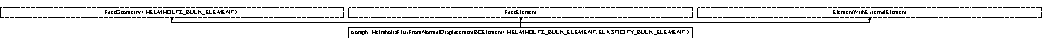
\includegraphics[height=0.612022cm]{classoomph_1_1HelmholtzFluxFromNormalDisplacementBCElement}
\end{center}
\end{figure}
\subsection*{Public Member Functions}
\begin{DoxyCompactItemize}
\item 
\hyperlink{classoomph_1_1HelmholtzFluxFromNormalDisplacementBCElement_ae37a7a8b5ad9850527f9285f2325aa2c}{Helmholtz\+Flux\+From\+Normal\+Displacement\+B\+C\+Element} (\hyperlink{classoomph_1_1FiniteElement}{Finite\+Element} $\ast$const \&bulk\+\_\+el\+\_\+pt, const int \&\hyperlink{classoomph_1_1FaceElement_a478d577ac6db67ecc80f1f02ae3ab170}{face\+\_\+index})
\begin{DoxyCompactList}\small\item\em Constructor, takes the pointer to the \char`\"{}bulk\char`\"{} element and the face index identifying the face to which the element is attached. \end{DoxyCompactList}\item 
\hyperlink{classoomph_1_1HelmholtzFluxFromNormalDisplacementBCElement_a5c093c485f9df81a14729f2ef41eced1}{Helmholtz\+Flux\+From\+Normal\+Displacement\+B\+C\+Element} (const \hyperlink{classoomph_1_1HelmholtzFluxFromNormalDisplacementBCElement}{Helmholtz\+Flux\+From\+Normal\+Displacement\+B\+C\+Element} \&dummy)
\begin{DoxyCompactList}\small\item\em Broken copy constructor. \end{DoxyCompactList}\item 
void \hyperlink{classoomph_1_1HelmholtzFluxFromNormalDisplacementBCElement_aab5bbb5d7c84d2aa0a5d9112e6f2d914}{fill\+\_\+in\+\_\+contribution\+\_\+to\+\_\+residuals} (\hyperlink{classoomph_1_1Vector}{Vector}$<$ double $>$ \&residuals)
\begin{DoxyCompactList}\small\item\em Broken assignment operator. \end{DoxyCompactList}\item 
void \hyperlink{classoomph_1_1HelmholtzFluxFromNormalDisplacementBCElement_a5e10f6e632c05ce464548f51c8381b43}{fill\+\_\+in\+\_\+contribution\+\_\+to\+\_\+jacobian} (\hyperlink{classoomph_1_1Vector}{Vector}$<$ double $>$ \&residuals, \hyperlink{classoomph_1_1DenseMatrix}{Dense\+Matrix}$<$ double $>$ \&jacobian)
\begin{DoxyCompactList}\small\item\em Add the element\textquotesingle{}s contribution to its residual vector and its Jacobian matrix. \end{DoxyCompactList}\item 
void \hyperlink{classoomph_1_1HelmholtzFluxFromNormalDisplacementBCElement_a778e21256d01c8b51e4d9ab8e5767d5f}{output} (std\+::ostream \&outfile)
\begin{DoxyCompactList}\small\item\em Output function. \end{DoxyCompactList}\item 
void \hyperlink{classoomph_1_1HelmholtzFluxFromNormalDisplacementBCElement_aec87ba2999b0c2e58447ca490b987c0e}{output} (std\+::ostream \&outfile, const unsigned \&n\+\_\+plot)
\begin{DoxyCompactList}\small\item\em Output function\+: flux etc at \hyperlink{classoomph_1_1Gauss}{Gauss} points; n\+\_\+plot is ignored. \end{DoxyCompactList}\item 
void \hyperlink{classoomph_1_1HelmholtzFluxFromNormalDisplacementBCElement_ae75706159d926cbad94fe66fa607b1fe}{output} (F\+I\+LE $\ast$file\+\_\+pt)
\begin{DoxyCompactList}\small\item\em C-\/style output function. \end{DoxyCompactList}\item 
void \hyperlink{classoomph_1_1HelmholtzFluxFromNormalDisplacementBCElement_a3a08931249b5071b11ec8082848cc94e}{output} (F\+I\+LE $\ast$file\+\_\+pt, const unsigned \&n\+\_\+plot)
\begin{DoxyCompactList}\small\item\em C-\/style output function. \end{DoxyCompactList}\end{DoxyCompactItemize}
\subsection*{Protected Member Functions}
\begin{DoxyCompactItemize}
\item 
double \hyperlink{classoomph_1_1HelmholtzFluxFromNormalDisplacementBCElement_a91ee0e36a8c127d83269a08d6740dfb2}{shape\+\_\+and\+\_\+test} (const \hyperlink{classoomph_1_1Vector}{Vector}$<$ double $>$ \&\hyperlink{cfortran_8h_ab7123126e4885ef647dd9c6e3807a21c}{s}, \hyperlink{classoomph_1_1Shape}{Shape} \&psi, \hyperlink{classoomph_1_1Shape}{Shape} \&test) const
\begin{DoxyCompactList}\small\item\em Function to compute the shape and test functions and to return the Jacobian of mapping between local and global (Eulerian) coordinates. \end{DoxyCompactList}\item 
double \hyperlink{classoomph_1_1HelmholtzFluxFromNormalDisplacementBCElement_ad3a879cf569b317c086f07872164f9f8}{shape\+\_\+and\+\_\+test\+\_\+at\+\_\+knot} (const unsigned \&ipt, \hyperlink{classoomph_1_1Shape}{Shape} \&psi, \hyperlink{classoomph_1_1Shape}{Shape} \&test) const
\begin{DoxyCompactList}\small\item\em Function to compute the shape and test functions and to return. \end{DoxyCompactList}\end{DoxyCompactItemize}
\subsection*{Private Member Functions}
\begin{DoxyCompactItemize}
\item 
void \hyperlink{classoomph_1_1HelmholtzFluxFromNormalDisplacementBCElement_a66f653fb85249296deb66cc91647cc52}{fill\+\_\+in\+\_\+generic\+\_\+residual\+\_\+contribution\+\_\+helmholtz\+\_\+flux\+\_\+from\+\_\+displacement} (\hyperlink{classoomph_1_1Vector}{Vector}$<$ double $>$ \&residuals, \hyperlink{classoomph_1_1DenseMatrix}{Dense\+Matrix}$<$ double $>$ \&jacobian, const unsigned \&flag)
\begin{DoxyCompactList}\small\item\em Add the element\textquotesingle{}s contribution to its residual vector. flag=1(or 0)\+: do (or don\textquotesingle{}t) compute the contribution to the Jacobian as well. \end{DoxyCompactList}\end{DoxyCompactItemize}
\subsection*{Private Attributes}
\begin{DoxyCompactItemize}
\item 
unsigned \hyperlink{classoomph_1_1HelmholtzFluxFromNormalDisplacementBCElement_a72d189d7598def4ce0ce2aecdc93bcd9}{Dim}
\begin{DoxyCompactList}\small\item\em The spatial dimension of the problem. \end{DoxyCompactList}\item 
std\+::complex$<$ unsigned $>$ \hyperlink{classoomph_1_1HelmholtzFluxFromNormalDisplacementBCElement_a84343ef8842d932061e696fdbd032590}{U\+\_\+index\+\_\+helmholtz\+\_\+from\+\_\+displacement}
\begin{DoxyCompactList}\small\item\em The index at which the unknown is stored at the nodes. \end{DoxyCompactList}\end{DoxyCompactItemize}
\subsection*{Additional Inherited Members}


\subsection{Detailed Description}
\subsubsection*{template$<$class H\+E\+L\+M\+H\+O\+L\+T\+Z\+\_\+\+B\+U\+L\+K\+\_\+\+E\+L\+E\+M\+E\+NT, class E\+L\+A\+S\+T\+I\+C\+I\+T\+Y\+\_\+\+B\+U\+L\+K\+\_\+\+E\+L\+E\+M\+E\+NT$>$\newline
class oomph\+::\+Helmholtz\+Flux\+From\+Normal\+Displacement\+B\+C\+Element$<$ H\+E\+L\+M\+H\+O\+L\+T\+Z\+\_\+\+B\+U\+L\+K\+\_\+\+E\+L\+E\+M\+E\+N\+T, E\+L\+A\+S\+T\+I\+C\+I\+T\+Y\+\_\+\+B\+U\+L\+K\+\_\+\+E\+L\+E\+M\+E\+N\+T $>$}

A class for elements that allow the imposition of an prescribed flux (determined from the normal displacements of an adjacent linearly elastic solid. Normal derivative for displacement potential is given by normal displacement of adjacent solid multiplies by F\+SI parameter (q = k$^\wedge$2 B/E). The element geometry is obtained from the Face\+Geometry$<$\+E\+L\+E\+M\+E\+N\+T$>$ policy class. 

Definition at line 456 of file helmholtz\+\_\+time\+\_\+harmonic\+\_\+linear\+\_\+elasticity\+\_\+interaction.\+h.



\subsection{Constructor \& Destructor Documentation}
\mbox{\Hypertarget{classoomph_1_1HelmholtzFluxFromNormalDisplacementBCElement_ae37a7a8b5ad9850527f9285f2325aa2c}\label{classoomph_1_1HelmholtzFluxFromNormalDisplacementBCElement_ae37a7a8b5ad9850527f9285f2325aa2c}} 
\index{oomph\+::\+Helmholtz\+Flux\+From\+Normal\+Displacement\+B\+C\+Element@{oomph\+::\+Helmholtz\+Flux\+From\+Normal\+Displacement\+B\+C\+Element}!Helmholtz\+Flux\+From\+Normal\+Displacement\+B\+C\+Element@{Helmholtz\+Flux\+From\+Normal\+Displacement\+B\+C\+Element}}
\index{Helmholtz\+Flux\+From\+Normal\+Displacement\+B\+C\+Element@{Helmholtz\+Flux\+From\+Normal\+Displacement\+B\+C\+Element}!oomph\+::\+Helmholtz\+Flux\+From\+Normal\+Displacement\+B\+C\+Element@{oomph\+::\+Helmholtz\+Flux\+From\+Normal\+Displacement\+B\+C\+Element}}
\subsubsection{\texorpdfstring{Helmholtz\+Flux\+From\+Normal\+Displacement\+B\+C\+Element()}{HelmholtzFluxFromNormalDisplacementBCElement()}\hspace{0.1cm}{\footnotesize\ttfamily [1/2]}}
{\footnotesize\ttfamily template$<$class H\+E\+L\+M\+H\+O\+L\+T\+Z\+\_\+\+B\+U\+L\+K\+\_\+\+E\+L\+E\+M\+E\+NT , class E\+L\+A\+S\+T\+I\+C\+I\+T\+Y\+\_\+\+B\+U\+L\+K\+\_\+\+E\+L\+E\+M\+E\+NT $>$ \\
\hyperlink{classoomph_1_1HelmholtzFluxFromNormalDisplacementBCElement}{oomph\+::\+Helmholtz\+Flux\+From\+Normal\+Displacement\+B\+C\+Element}$<$ H\+E\+L\+M\+H\+O\+L\+T\+Z\+\_\+\+B\+U\+L\+K\+\_\+\+E\+L\+E\+M\+E\+NT, E\+L\+A\+S\+T\+I\+C\+I\+T\+Y\+\_\+\+B\+U\+L\+K\+\_\+\+E\+L\+E\+M\+E\+NT $>$\+::\hyperlink{classoomph_1_1HelmholtzFluxFromNormalDisplacementBCElement}{Helmholtz\+Flux\+From\+Normal\+Displacement\+B\+C\+Element} (\begin{DoxyParamCaption}\item[{\hyperlink{classoomph_1_1FiniteElement}{Finite\+Element} $\ast$const \&}]{bulk\+\_\+el\+\_\+pt,  }\item[{const int \&}]{face\+\_\+index }\end{DoxyParamCaption})}



Constructor, takes the pointer to the \char`\"{}bulk\char`\"{} element and the face index identifying the face to which the element is attached. 

Constructor, takes the pointer to the \char`\"{}bulk\char`\"{} element, and the face index that identifies the face of the bulk element to which this face element is to be attached. 

Definition at line 669 of file helmholtz\+\_\+time\+\_\+harmonic\+\_\+linear\+\_\+elasticity\+\_\+interaction.\+h.



References oomph\+::\+Finite\+Element\+::build\+\_\+face\+\_\+element(), oomph\+::\+Helmholtz\+Flux\+From\+Normal\+Displacement\+B\+C\+Element$<$ H\+E\+L\+M\+H\+O\+L\+T\+Z\+\_\+\+B\+U\+L\+K\+\_\+\+E\+L\+E\+M\+E\+N\+T, E\+L\+A\+S\+T\+I\+C\+I\+T\+Y\+\_\+\+B\+U\+L\+K\+\_\+\+E\+L\+E\+M\+E\+N\+T $>$\+::\+Dim, oomph\+::\+Helmholtz\+Flux\+From\+Normal\+Displacement\+B\+C\+Element$<$ H\+E\+L\+M\+H\+O\+L\+T\+Z\+\_\+\+B\+U\+L\+K\+\_\+\+E\+L\+E\+M\+E\+N\+T, E\+L\+A\+S\+T\+I\+C\+I\+T\+Y\+\_\+\+B\+U\+L\+K\+\_\+\+E\+L\+E\+M\+E\+N\+T $>$\+::fill\+\_\+in\+\_\+generic\+\_\+residual\+\_\+contribution\+\_\+helmholtz\+\_\+flux\+\_\+from\+\_\+displacement(), oomph\+::\+Finite\+Element\+::has\+\_\+hanging\+\_\+nodes(), oomph\+::\+Node\+::ndim(), oomph\+::\+Finite\+Element\+::node\+\_\+pt(), oomph\+::\+Element\+With\+External\+Element\+::set\+\_\+ninteraction(), oomph\+::\+Global\+\_\+string\+\_\+for\+\_\+annotation\+::string(), oomph\+::\+Helmholtz\+Equations$<$ D\+I\+M $>$\+::u\+\_\+index\+\_\+helmholtz(), and oomph\+::\+Helmholtz\+Flux\+From\+Normal\+Displacement\+B\+C\+Element$<$ H\+E\+L\+M\+H\+O\+L\+T\+Z\+\_\+\+B\+U\+L\+K\+\_\+\+E\+L\+E\+M\+E\+N\+T, E\+L\+A\+S\+T\+I\+C\+I\+T\+Y\+\_\+\+B\+U\+L\+K\+\_\+\+E\+L\+E\+M\+E\+N\+T $>$\+::\+U\+\_\+index\+\_\+helmholtz\+\_\+from\+\_\+displacement.

\mbox{\Hypertarget{classoomph_1_1HelmholtzFluxFromNormalDisplacementBCElement_a5c093c485f9df81a14729f2ef41eced1}\label{classoomph_1_1HelmholtzFluxFromNormalDisplacementBCElement_a5c093c485f9df81a14729f2ef41eced1}} 
\index{oomph\+::\+Helmholtz\+Flux\+From\+Normal\+Displacement\+B\+C\+Element@{oomph\+::\+Helmholtz\+Flux\+From\+Normal\+Displacement\+B\+C\+Element}!Helmholtz\+Flux\+From\+Normal\+Displacement\+B\+C\+Element@{Helmholtz\+Flux\+From\+Normal\+Displacement\+B\+C\+Element}}
\index{Helmholtz\+Flux\+From\+Normal\+Displacement\+B\+C\+Element@{Helmholtz\+Flux\+From\+Normal\+Displacement\+B\+C\+Element}!oomph\+::\+Helmholtz\+Flux\+From\+Normal\+Displacement\+B\+C\+Element@{oomph\+::\+Helmholtz\+Flux\+From\+Normal\+Displacement\+B\+C\+Element}}
\subsubsection{\texorpdfstring{Helmholtz\+Flux\+From\+Normal\+Displacement\+B\+C\+Element()}{HelmholtzFluxFromNormalDisplacementBCElement()}\hspace{0.1cm}{\footnotesize\ttfamily [2/2]}}
{\footnotesize\ttfamily template$<$class H\+E\+L\+M\+H\+O\+L\+T\+Z\+\_\+\+B\+U\+L\+K\+\_\+\+E\+L\+E\+M\+E\+NT , class E\+L\+A\+S\+T\+I\+C\+I\+T\+Y\+\_\+\+B\+U\+L\+K\+\_\+\+E\+L\+E\+M\+E\+NT $>$ \\
\hyperlink{classoomph_1_1HelmholtzFluxFromNormalDisplacementBCElement}{oomph\+::\+Helmholtz\+Flux\+From\+Normal\+Displacement\+B\+C\+Element}$<$ H\+E\+L\+M\+H\+O\+L\+T\+Z\+\_\+\+B\+U\+L\+K\+\_\+\+E\+L\+E\+M\+E\+NT, E\+L\+A\+S\+T\+I\+C\+I\+T\+Y\+\_\+\+B\+U\+L\+K\+\_\+\+E\+L\+E\+M\+E\+NT $>$\+::\hyperlink{classoomph_1_1HelmholtzFluxFromNormalDisplacementBCElement}{Helmholtz\+Flux\+From\+Normal\+Displacement\+B\+C\+Element} (\begin{DoxyParamCaption}\item[{const \hyperlink{classoomph_1_1HelmholtzFluxFromNormalDisplacementBCElement}{Helmholtz\+Flux\+From\+Normal\+Displacement\+B\+C\+Element}$<$ H\+E\+L\+M\+H\+O\+L\+T\+Z\+\_\+\+B\+U\+L\+K\+\_\+\+E\+L\+E\+M\+E\+NT, E\+L\+A\+S\+T\+I\+C\+I\+T\+Y\+\_\+\+B\+U\+L\+K\+\_\+\+E\+L\+E\+M\+E\+NT $>$ \&}]{dummy }\end{DoxyParamCaption})\hspace{0.3cm}{\ttfamily [inline]}}



Broken copy constructor. 



Definition at line 471 of file helmholtz\+\_\+time\+\_\+harmonic\+\_\+linear\+\_\+elasticity\+\_\+interaction.\+h.



References oomph\+::\+Broken\+Copy\+::broken\+\_\+copy().



\subsection{Member Function Documentation}
\mbox{\Hypertarget{classoomph_1_1HelmholtzFluxFromNormalDisplacementBCElement_a5e10f6e632c05ce464548f51c8381b43}\label{classoomph_1_1HelmholtzFluxFromNormalDisplacementBCElement_a5e10f6e632c05ce464548f51c8381b43}} 
\index{oomph\+::\+Helmholtz\+Flux\+From\+Normal\+Displacement\+B\+C\+Element@{oomph\+::\+Helmholtz\+Flux\+From\+Normal\+Displacement\+B\+C\+Element}!fill\+\_\+in\+\_\+contribution\+\_\+to\+\_\+jacobian@{fill\+\_\+in\+\_\+contribution\+\_\+to\+\_\+jacobian}}
\index{fill\+\_\+in\+\_\+contribution\+\_\+to\+\_\+jacobian@{fill\+\_\+in\+\_\+contribution\+\_\+to\+\_\+jacobian}!oomph\+::\+Helmholtz\+Flux\+From\+Normal\+Displacement\+B\+C\+Element@{oomph\+::\+Helmholtz\+Flux\+From\+Normal\+Displacement\+B\+C\+Element}}
\subsubsection{\texorpdfstring{fill\+\_\+in\+\_\+contribution\+\_\+to\+\_\+jacobian()}{fill\_in\_contribution\_to\_jacobian()}}
{\footnotesize\ttfamily template$<$class H\+E\+L\+M\+H\+O\+L\+T\+Z\+\_\+\+B\+U\+L\+K\+\_\+\+E\+L\+E\+M\+E\+NT , class E\+L\+A\+S\+T\+I\+C\+I\+T\+Y\+\_\+\+B\+U\+L\+K\+\_\+\+E\+L\+E\+M\+E\+NT $>$ \\
void \hyperlink{classoomph_1_1HelmholtzFluxFromNormalDisplacementBCElement}{oomph\+::\+Helmholtz\+Flux\+From\+Normal\+Displacement\+B\+C\+Element}$<$ H\+E\+L\+M\+H\+O\+L\+T\+Z\+\_\+\+B\+U\+L\+K\+\_\+\+E\+L\+E\+M\+E\+NT, E\+L\+A\+S\+T\+I\+C\+I\+T\+Y\+\_\+\+B\+U\+L\+K\+\_\+\+E\+L\+E\+M\+E\+NT $>$\+::fill\+\_\+in\+\_\+contribution\+\_\+to\+\_\+jacobian (\begin{DoxyParamCaption}\item[{\hyperlink{classoomph_1_1Vector}{Vector}$<$ double $>$ \&}]{residuals,  }\item[{\hyperlink{classoomph_1_1DenseMatrix}{Dense\+Matrix}$<$ double $>$ \&}]{jacobian }\end{DoxyParamCaption})\hspace{0.3cm}{\ttfamily [inline]}, {\ttfamily [virtual]}}



Add the element\textquotesingle{}s contribution to its residual vector and its Jacobian matrix. 



Reimplemented from \hyperlink{classoomph_1_1ElementWithExternalElement_ae5fb09552a8271e891438f8d058ca1b8}{oomph\+::\+Element\+With\+External\+Element}.



Definition at line 500 of file helmholtz\+\_\+time\+\_\+harmonic\+\_\+linear\+\_\+elasticity\+\_\+interaction.\+h.



References oomph\+::\+Element\+With\+External\+Element\+::fill\+\_\+in\+\_\+jacobian\+\_\+from\+\_\+external\+\_\+interaction\+\_\+by\+\_\+fd().

\mbox{\Hypertarget{classoomph_1_1HelmholtzFluxFromNormalDisplacementBCElement_aab5bbb5d7c84d2aa0a5d9112e6f2d914}\label{classoomph_1_1HelmholtzFluxFromNormalDisplacementBCElement_aab5bbb5d7c84d2aa0a5d9112e6f2d914}} 
\index{oomph\+::\+Helmholtz\+Flux\+From\+Normal\+Displacement\+B\+C\+Element@{oomph\+::\+Helmholtz\+Flux\+From\+Normal\+Displacement\+B\+C\+Element}!fill\+\_\+in\+\_\+contribution\+\_\+to\+\_\+residuals@{fill\+\_\+in\+\_\+contribution\+\_\+to\+\_\+residuals}}
\index{fill\+\_\+in\+\_\+contribution\+\_\+to\+\_\+residuals@{fill\+\_\+in\+\_\+contribution\+\_\+to\+\_\+residuals}!oomph\+::\+Helmholtz\+Flux\+From\+Normal\+Displacement\+B\+C\+Element@{oomph\+::\+Helmholtz\+Flux\+From\+Normal\+Displacement\+B\+C\+Element}}
\subsubsection{\texorpdfstring{fill\+\_\+in\+\_\+contribution\+\_\+to\+\_\+residuals()}{fill\_in\_contribution\_to\_residuals()}}
{\footnotesize\ttfamily template$<$class H\+E\+L\+M\+H\+O\+L\+T\+Z\+\_\+\+B\+U\+L\+K\+\_\+\+E\+L\+E\+M\+E\+NT , class E\+L\+A\+S\+T\+I\+C\+I\+T\+Y\+\_\+\+B\+U\+L\+K\+\_\+\+E\+L\+E\+M\+E\+NT $>$ \\
void \hyperlink{classoomph_1_1HelmholtzFluxFromNormalDisplacementBCElement}{oomph\+::\+Helmholtz\+Flux\+From\+Normal\+Displacement\+B\+C\+Element}$<$ H\+E\+L\+M\+H\+O\+L\+T\+Z\+\_\+\+B\+U\+L\+K\+\_\+\+E\+L\+E\+M\+E\+NT, E\+L\+A\+S\+T\+I\+C\+I\+T\+Y\+\_\+\+B\+U\+L\+K\+\_\+\+E\+L\+E\+M\+E\+NT $>$\+::fill\+\_\+in\+\_\+contribution\+\_\+to\+\_\+residuals (\begin{DoxyParamCaption}\item[{\hyperlink{classoomph_1_1Vector}{Vector}$<$ double $>$ \&}]{residuals }\end{DoxyParamCaption})\hspace{0.3cm}{\ttfamily [inline]}, {\ttfamily [virtual]}}



Broken assignment operator. 

Add the element\textquotesingle{}s contribution to its residual vector 

Reimplemented from \hyperlink{classoomph_1_1GeneralisedElement_a310c97f515e8504a48179c0e72c550d7}{oomph\+::\+Generalised\+Element}.



Definition at line 489 of file helmholtz\+\_\+time\+\_\+harmonic\+\_\+linear\+\_\+elasticity\+\_\+interaction.\+h.



References oomph\+::\+Generalised\+Element\+::\+Dummy\+\_\+matrix.

\mbox{\Hypertarget{classoomph_1_1HelmholtzFluxFromNormalDisplacementBCElement_a66f653fb85249296deb66cc91647cc52}\label{classoomph_1_1HelmholtzFluxFromNormalDisplacementBCElement_a66f653fb85249296deb66cc91647cc52}} 
\index{oomph\+::\+Helmholtz\+Flux\+From\+Normal\+Displacement\+B\+C\+Element@{oomph\+::\+Helmholtz\+Flux\+From\+Normal\+Displacement\+B\+C\+Element}!fill\+\_\+in\+\_\+generic\+\_\+residual\+\_\+contribution\+\_\+helmholtz\+\_\+flux\+\_\+from\+\_\+displacement@{fill\+\_\+in\+\_\+generic\+\_\+residual\+\_\+contribution\+\_\+helmholtz\+\_\+flux\+\_\+from\+\_\+displacement}}
\index{fill\+\_\+in\+\_\+generic\+\_\+residual\+\_\+contribution\+\_\+helmholtz\+\_\+flux\+\_\+from\+\_\+displacement@{fill\+\_\+in\+\_\+generic\+\_\+residual\+\_\+contribution\+\_\+helmholtz\+\_\+flux\+\_\+from\+\_\+displacement}!oomph\+::\+Helmholtz\+Flux\+From\+Normal\+Displacement\+B\+C\+Element@{oomph\+::\+Helmholtz\+Flux\+From\+Normal\+Displacement\+B\+C\+Element}}
\subsubsection{\texorpdfstring{fill\+\_\+in\+\_\+generic\+\_\+residual\+\_\+contribution\+\_\+helmholtz\+\_\+flux\+\_\+from\+\_\+displacement()}{fill\_in\_generic\_residual\_contribution\_helmholtz\_flux\_from\_displacement()}}
{\footnotesize\ttfamily template$<$class H\+E\+L\+M\+H\+O\+L\+T\+Z\+\_\+\+B\+U\+L\+K\+\_\+\+E\+L\+E\+M\+E\+NT , class E\+L\+A\+S\+T\+I\+C\+I\+T\+Y\+\_\+\+B\+U\+L\+K\+\_\+\+E\+L\+E\+M\+E\+NT $>$ \\
void \hyperlink{classoomph_1_1HelmholtzFluxFromNormalDisplacementBCElement}{oomph\+::\+Helmholtz\+Flux\+From\+Normal\+Displacement\+B\+C\+Element}$<$ H\+E\+L\+M\+H\+O\+L\+T\+Z\+\_\+\+B\+U\+L\+K\+\_\+\+E\+L\+E\+M\+E\+NT, E\+L\+A\+S\+T\+I\+C\+I\+T\+Y\+\_\+\+B\+U\+L\+K\+\_\+\+E\+L\+E\+M\+E\+NT $>$\+::fill\+\_\+in\+\_\+generic\+\_\+residual\+\_\+contribution\+\_\+helmholtz\+\_\+flux\+\_\+from\+\_\+displacement (\begin{DoxyParamCaption}\item[{\hyperlink{classoomph_1_1Vector}{Vector}$<$ double $>$ \&}]{residuals,  }\item[{\hyperlink{classoomph_1_1DenseMatrix}{Dense\+Matrix}$<$ double $>$ \&}]{jacobian,  }\item[{const unsigned \&}]{flag }\end{DoxyParamCaption})\hspace{0.3cm}{\ttfamily [private]}}



Add the element\textquotesingle{}s contribution to its residual vector. flag=1(or 0)\+: do (or don\textquotesingle{}t) compute the contribution to the Jacobian as well. 

Helper function to compute the element\textquotesingle{}s residual vector and the Jacobian matrix. 

Definition at line 836 of file helmholtz\+\_\+time\+\_\+harmonic\+\_\+linear\+\_\+elasticity\+\_\+interaction.\+h.



References oomph\+::\+Helmholtz\+Flux\+From\+Normal\+Displacement\+B\+C\+Element$<$ H\+E\+L\+M\+H\+O\+L\+T\+Z\+\_\+\+B\+U\+L\+K\+\_\+\+E\+L\+E\+M\+E\+N\+T, E\+L\+A\+S\+T\+I\+C\+I\+T\+Y\+\_\+\+B\+U\+L\+K\+\_\+\+E\+L\+E\+M\+E\+N\+T $>$\+::\+Dim, oomph\+::\+Element\+With\+External\+Element\+::external\+\_\+element\+\_\+local\+\_\+coord(), oomph\+::\+Element\+With\+External\+Element\+::external\+\_\+element\+\_\+pt(), i, oomph\+::\+Finite\+Element\+::integral\+\_\+pt(), oomph\+::\+Face\+Element\+::interpolated\+\_\+x(), oomph\+::\+Integral\+::knot(), oomph\+::\+Finite\+Element\+::nnode(), oomph\+::\+Finite\+Element\+::nodal\+\_\+local\+\_\+eqn(), oomph\+::\+Finite\+Element\+::nodal\+\_\+position(), oomph\+::\+Integral\+::nweight(), oomph\+::\+Face\+Element\+::outer\+\_\+unit\+\_\+normal(), s, oomph\+::\+Helmholtz\+Flux\+From\+Normal\+Displacement\+B\+C\+Element$<$ H\+E\+L\+M\+H\+O\+L\+T\+Z\+\_\+\+B\+U\+L\+K\+\_\+\+E\+L\+E\+M\+E\+N\+T, E\+L\+A\+S\+T\+I\+C\+I\+T\+Y\+\_\+\+B\+U\+L\+K\+\_\+\+E\+L\+E\+M\+E\+N\+T $>$\+::shape\+\_\+and\+\_\+test(), oomph\+::\+Helmholtz\+Flux\+From\+Normal\+Displacement\+B\+C\+Element$<$ H\+E\+L\+M\+H\+O\+L\+T\+Z\+\_\+\+B\+U\+L\+K\+\_\+\+E\+L\+E\+M\+E\+N\+T, E\+L\+A\+S\+T\+I\+C\+I\+T\+Y\+\_\+\+B\+U\+L\+K\+\_\+\+E\+L\+E\+M\+E\+N\+T $>$\+::\+U\+\_\+index\+\_\+helmholtz\+\_\+from\+\_\+displacement, oomph\+::\+Quad\+Tree\+Names\+::W, and oomph\+::\+Integral\+::weight().



Referenced by oomph\+::\+Helmholtz\+Flux\+From\+Normal\+Displacement\+B\+C\+Element$<$ H\+E\+L\+M\+H\+O\+L\+T\+Z\+\_\+\+B\+U\+L\+K\+\_\+\+E\+L\+E\+M\+E\+N\+T, E\+L\+A\+S\+T\+I\+C\+I\+T\+Y\+\_\+\+B\+U\+L\+K\+\_\+\+E\+L\+E\+M\+E\+N\+T $>$\+::\+Helmholtz\+Flux\+From\+Normal\+Displacement\+B\+C\+Element().

\mbox{\Hypertarget{classoomph_1_1HelmholtzFluxFromNormalDisplacementBCElement_a778e21256d01c8b51e4d9ab8e5767d5f}\label{classoomph_1_1HelmholtzFluxFromNormalDisplacementBCElement_a778e21256d01c8b51e4d9ab8e5767d5f}} 
\index{oomph\+::\+Helmholtz\+Flux\+From\+Normal\+Displacement\+B\+C\+Element@{oomph\+::\+Helmholtz\+Flux\+From\+Normal\+Displacement\+B\+C\+Element}!output@{output}}
\index{output@{output}!oomph\+::\+Helmholtz\+Flux\+From\+Normal\+Displacement\+B\+C\+Element@{oomph\+::\+Helmholtz\+Flux\+From\+Normal\+Displacement\+B\+C\+Element}}
\subsubsection{\texorpdfstring{output()}{output()}\hspace{0.1cm}{\footnotesize\ttfamily [1/4]}}
{\footnotesize\ttfamily template$<$class H\+E\+L\+M\+H\+O\+L\+T\+Z\+\_\+\+B\+U\+L\+K\+\_\+\+E\+L\+E\+M\+E\+NT , class E\+L\+A\+S\+T\+I\+C\+I\+T\+Y\+\_\+\+B\+U\+L\+K\+\_\+\+E\+L\+E\+M\+E\+NT $>$ \\
void \hyperlink{classoomph_1_1HelmholtzFluxFromNormalDisplacementBCElement}{oomph\+::\+Helmholtz\+Flux\+From\+Normal\+Displacement\+B\+C\+Element}$<$ H\+E\+L\+M\+H\+O\+L\+T\+Z\+\_\+\+B\+U\+L\+K\+\_\+\+E\+L\+E\+M\+E\+NT, E\+L\+A\+S\+T\+I\+C\+I\+T\+Y\+\_\+\+B\+U\+L\+K\+\_\+\+E\+L\+E\+M\+E\+NT $>$\+::output (\begin{DoxyParamCaption}\item[{std\+::ostream \&}]{outfile }\end{DoxyParamCaption})\hspace{0.3cm}{\ttfamily [inline]}, {\ttfamily [virtual]}}



Output function. 



Reimplemented from \hyperlink{classoomph_1_1FiniteElement_a2ad98a3d2ef4999f1bef62c0ff13f2a7}{oomph\+::\+Finite\+Element}.



Definition at line 512 of file helmholtz\+\_\+time\+\_\+harmonic\+\_\+linear\+\_\+elasticity\+\_\+interaction.\+h.



References oomph\+::\+Time\+Harmonic\+Lin\+Elast\+Loaded\+By\+Helmholtz\+Pressure\+B\+C\+Element$<$ E\+L\+A\+S\+T\+I\+C\+I\+T\+Y\+\_\+\+B\+U\+L\+K\+\_\+\+E\+L\+E\+M\+E\+N\+T, H\+E\+L\+M\+H\+O\+L\+T\+Z\+\_\+\+B\+U\+L\+K\+\_\+\+E\+L\+E\+M\+E\+N\+T $>$\+::output().

\mbox{\Hypertarget{classoomph_1_1HelmholtzFluxFromNormalDisplacementBCElement_aec87ba2999b0c2e58447ca490b987c0e}\label{classoomph_1_1HelmholtzFluxFromNormalDisplacementBCElement_aec87ba2999b0c2e58447ca490b987c0e}} 
\index{oomph\+::\+Helmholtz\+Flux\+From\+Normal\+Displacement\+B\+C\+Element@{oomph\+::\+Helmholtz\+Flux\+From\+Normal\+Displacement\+B\+C\+Element}!output@{output}}
\index{output@{output}!oomph\+::\+Helmholtz\+Flux\+From\+Normal\+Displacement\+B\+C\+Element@{oomph\+::\+Helmholtz\+Flux\+From\+Normal\+Displacement\+B\+C\+Element}}
\subsubsection{\texorpdfstring{output()}{output()}\hspace{0.1cm}{\footnotesize\ttfamily [2/4]}}
{\footnotesize\ttfamily template$<$class H\+E\+L\+M\+H\+O\+L\+T\+Z\+\_\+\+B\+U\+L\+K\+\_\+\+E\+L\+E\+M\+E\+NT , class E\+L\+A\+S\+T\+I\+C\+I\+T\+Y\+\_\+\+B\+U\+L\+K\+\_\+\+E\+L\+E\+M\+E\+NT $>$ \\
void \hyperlink{classoomph_1_1HelmholtzFluxFromNormalDisplacementBCElement}{oomph\+::\+Helmholtz\+Flux\+From\+Normal\+Displacement\+B\+C\+Element}$<$ H\+E\+L\+M\+H\+O\+L\+T\+Z\+\_\+\+B\+U\+L\+K\+\_\+\+E\+L\+E\+M\+E\+NT, E\+L\+A\+S\+T\+I\+C\+I\+T\+Y\+\_\+\+B\+U\+L\+K\+\_\+\+E\+L\+E\+M\+E\+NT $>$\+::output (\begin{DoxyParamCaption}\item[{std\+::ostream \&}]{outfile,  }\item[{const unsigned \&}]{n\+\_\+plot }\end{DoxyParamCaption})\hspace{0.3cm}{\ttfamily [inline]}, {\ttfamily [virtual]}}



Output function\+: flux etc at \hyperlink{classoomph_1_1Gauss}{Gauss} points; n\+\_\+plot is ignored. 



Reimplemented from \hyperlink{classoomph_1_1FiniteElement_afa9d9b2670f999b43e6679c9dd28c457}{oomph\+::\+Finite\+Element}.



Definition at line 520 of file helmholtz\+\_\+time\+\_\+harmonic\+\_\+linear\+\_\+elasticity\+\_\+interaction.\+h.



References oomph\+::\+Multi\+\_\+domain\+\_\+functions\+::\+Dim, oomph\+::\+Element\+With\+External\+Element\+::external\+\_\+element\+\_\+local\+\_\+coord(), oomph\+::\+Element\+With\+External\+Element\+::external\+\_\+element\+\_\+pt(), i, oomph\+::\+Finite\+Element\+::integral\+\_\+pt(), oomph\+::\+Face\+Element\+::interpolated\+\_\+x(), oomph\+::\+Finite\+Element\+::interpolated\+\_\+zeta(), oomph\+::\+Integral\+::knot(), oomph\+::\+Integral\+::nweight(), and oomph\+::\+Face\+Element\+::outer\+\_\+unit\+\_\+normal().

\mbox{\Hypertarget{classoomph_1_1HelmholtzFluxFromNormalDisplacementBCElement_ae75706159d926cbad94fe66fa607b1fe}\label{classoomph_1_1HelmholtzFluxFromNormalDisplacementBCElement_ae75706159d926cbad94fe66fa607b1fe}} 
\index{oomph\+::\+Helmholtz\+Flux\+From\+Normal\+Displacement\+B\+C\+Element@{oomph\+::\+Helmholtz\+Flux\+From\+Normal\+Displacement\+B\+C\+Element}!output@{output}}
\index{output@{output}!oomph\+::\+Helmholtz\+Flux\+From\+Normal\+Displacement\+B\+C\+Element@{oomph\+::\+Helmholtz\+Flux\+From\+Normal\+Displacement\+B\+C\+Element}}
\subsubsection{\texorpdfstring{output()}{output()}\hspace{0.1cm}{\footnotesize\ttfamily [3/4]}}
{\footnotesize\ttfamily template$<$class H\+E\+L\+M\+H\+O\+L\+T\+Z\+\_\+\+B\+U\+L\+K\+\_\+\+E\+L\+E\+M\+E\+NT , class E\+L\+A\+S\+T\+I\+C\+I\+T\+Y\+\_\+\+B\+U\+L\+K\+\_\+\+E\+L\+E\+M\+E\+NT $>$ \\
void \hyperlink{classoomph_1_1HelmholtzFluxFromNormalDisplacementBCElement}{oomph\+::\+Helmholtz\+Flux\+From\+Normal\+Displacement\+B\+C\+Element}$<$ H\+E\+L\+M\+H\+O\+L\+T\+Z\+\_\+\+B\+U\+L\+K\+\_\+\+E\+L\+E\+M\+E\+NT, E\+L\+A\+S\+T\+I\+C\+I\+T\+Y\+\_\+\+B\+U\+L\+K\+\_\+\+E\+L\+E\+M\+E\+NT $>$\+::output (\begin{DoxyParamCaption}\item[{F\+I\+LE $\ast$}]{file\+\_\+pt }\end{DoxyParamCaption})\hspace{0.3cm}{\ttfamily [inline]}, {\ttfamily [virtual]}}



C-\/style output function. 



Reimplemented from \hyperlink{classoomph_1_1FiniteElement_a72cddd09f8ddbee1a20a1ff404c6943e}{oomph\+::\+Finite\+Element}.



Definition at line 583 of file helmholtz\+\_\+time\+\_\+harmonic\+\_\+linear\+\_\+elasticity\+\_\+interaction.\+h.



References oomph\+::output().

\mbox{\Hypertarget{classoomph_1_1HelmholtzFluxFromNormalDisplacementBCElement_a3a08931249b5071b11ec8082848cc94e}\label{classoomph_1_1HelmholtzFluxFromNormalDisplacementBCElement_a3a08931249b5071b11ec8082848cc94e}} 
\index{oomph\+::\+Helmholtz\+Flux\+From\+Normal\+Displacement\+B\+C\+Element@{oomph\+::\+Helmholtz\+Flux\+From\+Normal\+Displacement\+B\+C\+Element}!output@{output}}
\index{output@{output}!oomph\+::\+Helmholtz\+Flux\+From\+Normal\+Displacement\+B\+C\+Element@{oomph\+::\+Helmholtz\+Flux\+From\+Normal\+Displacement\+B\+C\+Element}}
\subsubsection{\texorpdfstring{output()}{output()}\hspace{0.1cm}{\footnotesize\ttfamily [4/4]}}
{\footnotesize\ttfamily template$<$class H\+E\+L\+M\+H\+O\+L\+T\+Z\+\_\+\+B\+U\+L\+K\+\_\+\+E\+L\+E\+M\+E\+NT , class E\+L\+A\+S\+T\+I\+C\+I\+T\+Y\+\_\+\+B\+U\+L\+K\+\_\+\+E\+L\+E\+M\+E\+NT $>$ \\
void \hyperlink{classoomph_1_1HelmholtzFluxFromNormalDisplacementBCElement}{oomph\+::\+Helmholtz\+Flux\+From\+Normal\+Displacement\+B\+C\+Element}$<$ H\+E\+L\+M\+H\+O\+L\+T\+Z\+\_\+\+B\+U\+L\+K\+\_\+\+E\+L\+E\+M\+E\+NT, E\+L\+A\+S\+T\+I\+C\+I\+T\+Y\+\_\+\+B\+U\+L\+K\+\_\+\+E\+L\+E\+M\+E\+NT $>$\+::output (\begin{DoxyParamCaption}\item[{F\+I\+LE $\ast$}]{file\+\_\+pt,  }\item[{const unsigned \&}]{n\+\_\+plot }\end{DoxyParamCaption})\hspace{0.3cm}{\ttfamily [inline]}, {\ttfamily [virtual]}}



C-\/style output function. 



Reimplemented from \hyperlink{classoomph_1_1FiniteElement_adfaee690bb0608f03320eeb9d110d48c}{oomph\+::\+Finite\+Element}.



Definition at line 587 of file helmholtz\+\_\+time\+\_\+harmonic\+\_\+linear\+\_\+elasticity\+\_\+interaction.\+h.



References oomph\+::output().

\mbox{\Hypertarget{classoomph_1_1HelmholtzFluxFromNormalDisplacementBCElement_a91ee0e36a8c127d83269a08d6740dfb2}\label{classoomph_1_1HelmholtzFluxFromNormalDisplacementBCElement_a91ee0e36a8c127d83269a08d6740dfb2}} 
\index{oomph\+::\+Helmholtz\+Flux\+From\+Normal\+Displacement\+B\+C\+Element@{oomph\+::\+Helmholtz\+Flux\+From\+Normal\+Displacement\+B\+C\+Element}!shape\+\_\+and\+\_\+test@{shape\+\_\+and\+\_\+test}}
\index{shape\+\_\+and\+\_\+test@{shape\+\_\+and\+\_\+test}!oomph\+::\+Helmholtz\+Flux\+From\+Normal\+Displacement\+B\+C\+Element@{oomph\+::\+Helmholtz\+Flux\+From\+Normal\+Displacement\+B\+C\+Element}}
\subsubsection{\texorpdfstring{shape\+\_\+and\+\_\+test()}{shape\_and\_test()}}
{\footnotesize\ttfamily template$<$class H\+E\+L\+M\+H\+O\+L\+T\+Z\+\_\+\+B\+U\+L\+K\+\_\+\+E\+L\+E\+M\+E\+NT , class E\+L\+A\+S\+T\+I\+C\+I\+T\+Y\+\_\+\+B\+U\+L\+K\+\_\+\+E\+L\+E\+M\+E\+NT $>$ \\
double \hyperlink{classoomph_1_1HelmholtzFluxFromNormalDisplacementBCElement}{oomph\+::\+Helmholtz\+Flux\+From\+Normal\+Displacement\+B\+C\+Element}$<$ H\+E\+L\+M\+H\+O\+L\+T\+Z\+\_\+\+B\+U\+L\+K\+\_\+\+E\+L\+E\+M\+E\+NT, E\+L\+A\+S\+T\+I\+C\+I\+T\+Y\+\_\+\+B\+U\+L\+K\+\_\+\+E\+L\+E\+M\+E\+NT $>$\+::shape\+\_\+and\+\_\+test (\begin{DoxyParamCaption}\item[{const \hyperlink{classoomph_1_1Vector}{Vector}$<$ double $>$ \&}]{s,  }\item[{\hyperlink{classoomph_1_1Shape}{Shape} \&}]{psi,  }\item[{\hyperlink{classoomph_1_1Shape}{Shape} \&}]{test }\end{DoxyParamCaption}) const\hspace{0.3cm}{\ttfamily [inline]}, {\ttfamily [protected]}}



Function to compute the shape and test functions and to return the Jacobian of mapping between local and global (Eulerian) coordinates. 



Definition at line 597 of file helmholtz\+\_\+time\+\_\+harmonic\+\_\+linear\+\_\+elasticity\+\_\+interaction.\+h.



References i, oomph\+::\+Face\+Element\+::\+J\+\_\+eulerian(), oomph\+::\+Finite\+Element\+::nnode(), and oomph\+::\+Finite\+Element\+::shape().



Referenced by oomph\+::\+Helmholtz\+Flux\+From\+Normal\+Displacement\+B\+C\+Element$<$ H\+E\+L\+M\+H\+O\+L\+T\+Z\+\_\+\+B\+U\+L\+K\+\_\+\+E\+L\+E\+M\+E\+N\+T, E\+L\+A\+S\+T\+I\+C\+I\+T\+Y\+\_\+\+B\+U\+L\+K\+\_\+\+E\+L\+E\+M\+E\+N\+T $>$\+::fill\+\_\+in\+\_\+generic\+\_\+residual\+\_\+contribution\+\_\+helmholtz\+\_\+flux\+\_\+from\+\_\+displacement().

\mbox{\Hypertarget{classoomph_1_1HelmholtzFluxFromNormalDisplacementBCElement_ad3a879cf569b317c086f07872164f9f8}\label{classoomph_1_1HelmholtzFluxFromNormalDisplacementBCElement_ad3a879cf569b317c086f07872164f9f8}} 
\index{oomph\+::\+Helmholtz\+Flux\+From\+Normal\+Displacement\+B\+C\+Element@{oomph\+::\+Helmholtz\+Flux\+From\+Normal\+Displacement\+B\+C\+Element}!shape\+\_\+and\+\_\+test\+\_\+at\+\_\+knot@{shape\+\_\+and\+\_\+test\+\_\+at\+\_\+knot}}
\index{shape\+\_\+and\+\_\+test\+\_\+at\+\_\+knot@{shape\+\_\+and\+\_\+test\+\_\+at\+\_\+knot}!oomph\+::\+Helmholtz\+Flux\+From\+Normal\+Displacement\+B\+C\+Element@{oomph\+::\+Helmholtz\+Flux\+From\+Normal\+Displacement\+B\+C\+Element}}
\subsubsection{\texorpdfstring{shape\+\_\+and\+\_\+test\+\_\+at\+\_\+knot()}{shape\_and\_test\_at\_knot()}}
{\footnotesize\ttfamily template$<$class H\+E\+L\+M\+H\+O\+L\+T\+Z\+\_\+\+B\+U\+L\+K\+\_\+\+E\+L\+E\+M\+E\+NT , class E\+L\+A\+S\+T\+I\+C\+I\+T\+Y\+\_\+\+B\+U\+L\+K\+\_\+\+E\+L\+E\+M\+E\+NT $>$ \\
double \hyperlink{classoomph_1_1HelmholtzFluxFromNormalDisplacementBCElement}{oomph\+::\+Helmholtz\+Flux\+From\+Normal\+Displacement\+B\+C\+Element}$<$ H\+E\+L\+M\+H\+O\+L\+T\+Z\+\_\+\+B\+U\+L\+K\+\_\+\+E\+L\+E\+M\+E\+NT, E\+L\+A\+S\+T\+I\+C\+I\+T\+Y\+\_\+\+B\+U\+L\+K\+\_\+\+E\+L\+E\+M\+E\+NT $>$\+::shape\+\_\+and\+\_\+test\+\_\+at\+\_\+knot (\begin{DoxyParamCaption}\item[{const unsigned \&}]{ipt,  }\item[{\hyperlink{classoomph_1_1Shape}{Shape} \&}]{psi,  }\item[{\hyperlink{classoomph_1_1Shape}{Shape} \&}]{test }\end{DoxyParamCaption}) const\hspace{0.3cm}{\ttfamily [inline]}, {\ttfamily [protected]}}



Function to compute the shape and test functions and to return. 

the Jacobian of mapping between local and global (Eulerian) coordinates 

Definition at line 617 of file helmholtz\+\_\+time\+\_\+harmonic\+\_\+linear\+\_\+elasticity\+\_\+interaction.\+h.



References i, oomph\+::\+Face\+Element\+::\+J\+\_\+eulerian\+\_\+at\+\_\+knot(), oomph\+::\+Finite\+Element\+::nnode(), and oomph\+::\+Finite\+Element\+::shape\+\_\+at\+\_\+knot().



\subsection{Member Data Documentation}
\mbox{\Hypertarget{classoomph_1_1HelmholtzFluxFromNormalDisplacementBCElement_a72d189d7598def4ce0ce2aecdc93bcd9}\label{classoomph_1_1HelmholtzFluxFromNormalDisplacementBCElement_a72d189d7598def4ce0ce2aecdc93bcd9}} 
\index{oomph\+::\+Helmholtz\+Flux\+From\+Normal\+Displacement\+B\+C\+Element@{oomph\+::\+Helmholtz\+Flux\+From\+Normal\+Displacement\+B\+C\+Element}!Dim@{Dim}}
\index{Dim@{Dim}!oomph\+::\+Helmholtz\+Flux\+From\+Normal\+Displacement\+B\+C\+Element@{oomph\+::\+Helmholtz\+Flux\+From\+Normal\+Displacement\+B\+C\+Element}}
\subsubsection{\texorpdfstring{Dim}{Dim}}
{\footnotesize\ttfamily template$<$class H\+E\+L\+M\+H\+O\+L\+T\+Z\+\_\+\+B\+U\+L\+K\+\_\+\+E\+L\+E\+M\+E\+NT , class E\+L\+A\+S\+T\+I\+C\+I\+T\+Y\+\_\+\+B\+U\+L\+K\+\_\+\+E\+L\+E\+M\+E\+NT $>$ \\
unsigned \hyperlink{classoomph_1_1HelmholtzFluxFromNormalDisplacementBCElement}{oomph\+::\+Helmholtz\+Flux\+From\+Normal\+Displacement\+B\+C\+Element}$<$ H\+E\+L\+M\+H\+O\+L\+T\+Z\+\_\+\+B\+U\+L\+K\+\_\+\+E\+L\+E\+M\+E\+NT, E\+L\+A\+S\+T\+I\+C\+I\+T\+Y\+\_\+\+B\+U\+L\+K\+\_\+\+E\+L\+E\+M\+E\+NT $>$\+::Dim\hspace{0.3cm}{\ttfamily [private]}}



The spatial dimension of the problem. 



Definition at line 647 of file helmholtz\+\_\+time\+\_\+harmonic\+\_\+linear\+\_\+elasticity\+\_\+interaction.\+h.



Referenced by oomph\+::\+Helmholtz\+Flux\+From\+Normal\+Displacement\+B\+C\+Element$<$ H\+E\+L\+M\+H\+O\+L\+T\+Z\+\_\+\+B\+U\+L\+K\+\_\+\+E\+L\+E\+M\+E\+N\+T, E\+L\+A\+S\+T\+I\+C\+I\+T\+Y\+\_\+\+B\+U\+L\+K\+\_\+\+E\+L\+E\+M\+E\+N\+T $>$\+::fill\+\_\+in\+\_\+generic\+\_\+residual\+\_\+contribution\+\_\+helmholtz\+\_\+flux\+\_\+from\+\_\+displacement(), and oomph\+::\+Helmholtz\+Flux\+From\+Normal\+Displacement\+B\+C\+Element$<$ H\+E\+L\+M\+H\+O\+L\+T\+Z\+\_\+\+B\+U\+L\+K\+\_\+\+E\+L\+E\+M\+E\+N\+T, E\+L\+A\+S\+T\+I\+C\+I\+T\+Y\+\_\+\+B\+U\+L\+K\+\_\+\+E\+L\+E\+M\+E\+N\+T $>$\+::\+Helmholtz\+Flux\+From\+Normal\+Displacement\+B\+C\+Element().

\mbox{\Hypertarget{classoomph_1_1HelmholtzFluxFromNormalDisplacementBCElement_a84343ef8842d932061e696fdbd032590}\label{classoomph_1_1HelmholtzFluxFromNormalDisplacementBCElement_a84343ef8842d932061e696fdbd032590}} 
\index{oomph\+::\+Helmholtz\+Flux\+From\+Normal\+Displacement\+B\+C\+Element@{oomph\+::\+Helmholtz\+Flux\+From\+Normal\+Displacement\+B\+C\+Element}!U\+\_\+index\+\_\+helmholtz\+\_\+from\+\_\+displacement@{U\+\_\+index\+\_\+helmholtz\+\_\+from\+\_\+displacement}}
\index{U\+\_\+index\+\_\+helmholtz\+\_\+from\+\_\+displacement@{U\+\_\+index\+\_\+helmholtz\+\_\+from\+\_\+displacement}!oomph\+::\+Helmholtz\+Flux\+From\+Normal\+Displacement\+B\+C\+Element@{oomph\+::\+Helmholtz\+Flux\+From\+Normal\+Displacement\+B\+C\+Element}}
\subsubsection{\texorpdfstring{U\+\_\+index\+\_\+helmholtz\+\_\+from\+\_\+displacement}{U\_index\_helmholtz\_from\_displacement}}
{\footnotesize\ttfamily template$<$class H\+E\+L\+M\+H\+O\+L\+T\+Z\+\_\+\+B\+U\+L\+K\+\_\+\+E\+L\+E\+M\+E\+NT , class E\+L\+A\+S\+T\+I\+C\+I\+T\+Y\+\_\+\+B\+U\+L\+K\+\_\+\+E\+L\+E\+M\+E\+NT $>$ \\
std\+::complex$<$unsigned$>$ \hyperlink{classoomph_1_1HelmholtzFluxFromNormalDisplacementBCElement}{oomph\+::\+Helmholtz\+Flux\+From\+Normal\+Displacement\+B\+C\+Element}$<$ H\+E\+L\+M\+H\+O\+L\+T\+Z\+\_\+\+B\+U\+L\+K\+\_\+\+E\+L\+E\+M\+E\+NT, E\+L\+A\+S\+T\+I\+C\+I\+T\+Y\+\_\+\+B\+U\+L\+K\+\_\+\+E\+L\+E\+M\+E\+NT $>$\+::U\+\_\+index\+\_\+helmholtz\+\_\+from\+\_\+displacement\hspace{0.3cm}{\ttfamily [private]}}



The index at which the unknown is stored at the nodes. 



Definition at line 650 of file helmholtz\+\_\+time\+\_\+harmonic\+\_\+linear\+\_\+elasticity\+\_\+interaction.\+h.



Referenced by oomph\+::\+Helmholtz\+Flux\+From\+Normal\+Displacement\+B\+C\+Element$<$ H\+E\+L\+M\+H\+O\+L\+T\+Z\+\_\+\+B\+U\+L\+K\+\_\+\+E\+L\+E\+M\+E\+N\+T, E\+L\+A\+S\+T\+I\+C\+I\+T\+Y\+\_\+\+B\+U\+L\+K\+\_\+\+E\+L\+E\+M\+E\+N\+T $>$\+::fill\+\_\+in\+\_\+generic\+\_\+residual\+\_\+contribution\+\_\+helmholtz\+\_\+flux\+\_\+from\+\_\+displacement(), and oomph\+::\+Helmholtz\+Flux\+From\+Normal\+Displacement\+B\+C\+Element$<$ H\+E\+L\+M\+H\+O\+L\+T\+Z\+\_\+\+B\+U\+L\+K\+\_\+\+E\+L\+E\+M\+E\+N\+T, E\+L\+A\+S\+T\+I\+C\+I\+T\+Y\+\_\+\+B\+U\+L\+K\+\_\+\+E\+L\+E\+M\+E\+N\+T $>$\+::\+Helmholtz\+Flux\+From\+Normal\+Displacement\+B\+C\+Element().



The documentation for this class was generated from the following file\+:\begin{DoxyCompactItemize}
\item 
\hyperlink{helmholtz__time__harmonic__linear__elasticity__interaction_8h}{helmholtz\+\_\+time\+\_\+harmonic\+\_\+linear\+\_\+elasticity\+\_\+interaction.\+h}\end{DoxyCompactItemize}

\hypertarget{classoomph_1_1NavierStokesBoussinesqElement}{}\section{oomph\+:\+:Navier\+Stokes\+Boussinesq\+Element$<$ N\+S\+T\+\_\+\+E\+L\+E\+M\+E\+NT, A\+D\+\_\+\+E\+L\+E\+M\+E\+NT $>$ Class Template Reference}
\label{classoomph_1_1NavierStokesBoussinesqElement}\index{oomph\+::\+Navier\+Stokes\+Boussinesq\+Element$<$ N\+S\+T\+\_\+\+E\+L\+E\+M\+E\+N\+T, A\+D\+\_\+\+E\+L\+E\+M\+E\+N\+T $>$@{oomph\+::\+Navier\+Stokes\+Boussinesq\+Element$<$ N\+S\+T\+\_\+\+E\+L\+E\+M\+E\+N\+T, A\+D\+\_\+\+E\+L\+E\+M\+E\+N\+T $>$}}


{\ttfamily \#include $<$multi\+\_\+domain\+\_\+boussinesq\+\_\+elements.\+h$>$}

Inheritance diagram for oomph\+:\+:Navier\+Stokes\+Boussinesq\+Element$<$ N\+S\+T\+\_\+\+E\+L\+E\+M\+E\+NT, A\+D\+\_\+\+E\+L\+E\+M\+E\+NT $>$\+:\begin{figure}[H]
\begin{center}
\leavevmode
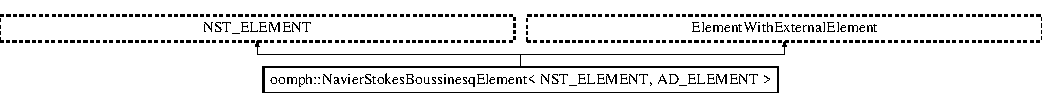
\includegraphics[height=1.659259cm]{classoomph_1_1NavierStokesBoussinesqElement}
\end{center}
\end{figure}
\subsection*{Public Member Functions}
\begin{DoxyCompactItemize}
\item 
\hyperlink{classoomph_1_1NavierStokesBoussinesqElement_ad0ebb74a3963c0715e6e3e34ba8b1d7f}{Navier\+Stokes\+Boussinesq\+Element} ()
\begin{DoxyCompactList}\small\item\em Constructor\+: call the underlying constructors and initialise the pointer to the Rayleigh number to point to the default value of 0.\+0. \end{DoxyCompactList}\item 
const double \& \hyperlink{classoomph_1_1NavierStokesBoussinesqElement_a3318acc1306c60bd13b3bfe8e15a2fa5}{ra} () const
\begin{DoxyCompactList}\small\item\em Access function for the Rayleigh number (const version) \end{DoxyCompactList}\item 
double $\ast$\& \hyperlink{classoomph_1_1NavierStokesBoussinesqElement_ac822ef74e7bc0e55c917e58f2cd5a6fe}{ra\+\_\+pt} ()
\begin{DoxyCompactList}\small\item\em Access function for the pointer to the Rayleigh number. \end{DoxyCompactList}\item 
void \hyperlink{classoomph_1_1NavierStokesBoussinesqElement_a2ff5be3155df975541a25444d43c1ca8}{get\+\_\+body\+\_\+force\+\_\+nst} (const double \&time, const unsigned \&ipt, const \hyperlink{classoomph_1_1Vector}{Vector}$<$ double $>$ \&\hyperlink{cfortran_8h_ab7123126e4885ef647dd9c6e3807a21c}{s}, const \hyperlink{classoomph_1_1Vector}{Vector}$<$ double $>$ \&x, \hyperlink{classoomph_1_1Vector}{Vector}$<$ double $>$ \&result)
\begin{DoxyCompactList}\small\item\em Overload get\+\_\+body\+\_\+force\+\_\+nst to get the temperature \char`\"{}body force\char`\"{} from the \char`\"{}source\char`\"{} Advection\+Diffusion element via current integration point. \end{DoxyCompactList}\item 
void \hyperlink{classoomph_1_1NavierStokesBoussinesqElement_a8a84c39e2156ab16b7aefc400891ac27}{get\+\_\+dbody\+\_\+force\+\_\+nst\+\_\+dexternal\+\_\+element\+\_\+data} (const unsigned \&ipt, \hyperlink{classoomph_1_1DenseMatrix}{Dense\+Matrix}$<$ double $>$ \&result, \hyperlink{classoomph_1_1Vector}{Vector}$<$ unsigned $>$ \&global\+\_\+eqn\+\_\+number)
\begin{DoxyCompactList}\small\item\em Fill in the derivatives of the body force with respect to the external unknowns. \end{DoxyCompactList}\item 
void \hyperlink{classoomph_1_1NavierStokesBoussinesqElement_a01483469b070309aeb8948273b974feb}{fill\+\_\+in\+\_\+contribution\+\_\+to\+\_\+jacobian} (\hyperlink{classoomph_1_1Vector}{Vector}$<$ double $>$ \&residuals, \hyperlink{classoomph_1_1DenseMatrix}{Dense\+Matrix}$<$ double $>$ \&jacobian)
\begin{DoxyCompactList}\small\item\em Compute the element\textquotesingle{}s residual vector and the Jacobian matrix. Jacobian is computed by finite-\/differencing or analytically. \end{DoxyCompactList}\item 
void \hyperlink{classoomph_1_1NavierStokesBoussinesqElement_a6c6cc7f75f0f9d61574293648bc4f148}{fill\+\_\+in\+\_\+contribution\+\_\+to\+\_\+jacobian\+\_\+and\+\_\+mass\+\_\+matrix} (\hyperlink{classoomph_1_1Vector}{Vector}$<$ double $>$ \&residuals, \hyperlink{classoomph_1_1DenseMatrix}{Dense\+Matrix}$<$ double $>$ \&jacobian, \hyperlink{classoomph_1_1DenseMatrix}{Dense\+Matrix}$<$ double $>$ \&mass\+\_\+matrix)
\begin{DoxyCompactList}\small\item\em Add the element\textquotesingle{}s contribution to its residuals vector, jacobian matrix and mass matrix. \end{DoxyCompactList}\item 
void \hyperlink{classoomph_1_1NavierStokesBoussinesqElement_a342613c3ceeaf4b5bb86c77dc150372d}{fill\+\_\+in\+\_\+off\+\_\+diagonal\+\_\+block\+\_\+analytic} (\hyperlink{classoomph_1_1Vector}{Vector}$<$ double $>$ \&residuals, \hyperlink{classoomph_1_1DenseMatrix}{Dense\+Matrix}$<$ double $>$ \&jacobian)
\begin{DoxyCompactList}\small\item\em Compute the contribution of the external degrees of freedom (temperatures) on the Navier-\/\+Stokes equations. \end{DoxyCompactList}\end{DoxyCompactItemize}
\subsection*{Private Attributes}
\begin{DoxyCompactItemize}
\item 
double $\ast$ \hyperlink{classoomph_1_1NavierStokesBoussinesqElement_a0f1c9b6947324c4d5386b9b68abba2d1}{Ra\+\_\+pt}
\begin{DoxyCompactList}\small\item\em Pointer to a private data member, the Rayleigh number. \end{DoxyCompactList}\end{DoxyCompactItemize}
\subsection*{Additional Inherited Members}


\subsection{Detailed Description}
\subsubsection*{template$<$class N\+S\+T\+\_\+\+E\+L\+E\+M\+E\+NT, class A\+D\+\_\+\+E\+L\+E\+M\+E\+NT$>$\newline
class oomph\+::\+Navier\+Stokes\+Boussinesq\+Element$<$ N\+S\+T\+\_\+\+E\+L\+E\+M\+E\+N\+T, A\+D\+\_\+\+E\+L\+E\+M\+E\+N\+T $>$}

Build \hyperlink{classoomph_1_1NavierStokesBoussinesqElement}{Navier\+Stokes\+Boussinesq\+Element} that inherits from \hyperlink{classoomph_1_1ElementWithExternalElement}{Element\+With\+External\+Element} so that it can \char`\"{}communicate\char`\"{} with Advection\+Diffusion\+Element\+With\+External\+Element 

Definition at line 809 of file multi\+\_\+domain\+\_\+boussinesq\+\_\+elements.\+h.



\subsection{Constructor \& Destructor Documentation}
\mbox{\Hypertarget{classoomph_1_1NavierStokesBoussinesqElement_ad0ebb74a3963c0715e6e3e34ba8b1d7f}\label{classoomph_1_1NavierStokesBoussinesqElement_ad0ebb74a3963c0715e6e3e34ba8b1d7f}} 
\index{oomph\+::\+Navier\+Stokes\+Boussinesq\+Element@{oomph\+::\+Navier\+Stokes\+Boussinesq\+Element}!Navier\+Stokes\+Boussinesq\+Element@{Navier\+Stokes\+Boussinesq\+Element}}
\index{Navier\+Stokes\+Boussinesq\+Element@{Navier\+Stokes\+Boussinesq\+Element}!oomph\+::\+Navier\+Stokes\+Boussinesq\+Element@{oomph\+::\+Navier\+Stokes\+Boussinesq\+Element}}
\subsubsection{\texorpdfstring{Navier\+Stokes\+Boussinesq\+Element()}{NavierStokesBoussinesqElement()}}
{\footnotesize\ttfamily template$<$class N\+S\+T\+\_\+\+E\+L\+E\+M\+E\+NT , class A\+D\+\_\+\+E\+L\+E\+M\+E\+NT $>$ \\
\hyperlink{classoomph_1_1NavierStokesBoussinesqElement}{oomph\+::\+Navier\+Stokes\+Boussinesq\+Element}$<$ N\+S\+T\+\_\+\+E\+L\+E\+M\+E\+NT, A\+D\+\_\+\+E\+L\+E\+M\+E\+NT $>$\+::\hyperlink{classoomph_1_1NavierStokesBoussinesqElement}{Navier\+Stokes\+Boussinesq\+Element} (\begin{DoxyParamCaption}{ }\end{DoxyParamCaption})\hspace{0.3cm}{\ttfamily [inline]}}



Constructor\+: call the underlying constructors and initialise the pointer to the Rayleigh number to point to the default value of 0.\+0. 



Definition at line 823 of file multi\+\_\+domain\+\_\+boussinesq\+\_\+elements.\+h.



References oomph\+::\+Multi\+Domain\+Boussinesq\+Helper\+::\+Default\+\_\+\+Physical\+\_\+\+Constant\+\_\+\+Value.



\subsection{Member Function Documentation}
\mbox{\Hypertarget{classoomph_1_1NavierStokesBoussinesqElement_a01483469b070309aeb8948273b974feb}\label{classoomph_1_1NavierStokesBoussinesqElement_a01483469b070309aeb8948273b974feb}} 
\index{oomph\+::\+Navier\+Stokes\+Boussinesq\+Element@{oomph\+::\+Navier\+Stokes\+Boussinesq\+Element}!fill\+\_\+in\+\_\+contribution\+\_\+to\+\_\+jacobian@{fill\+\_\+in\+\_\+contribution\+\_\+to\+\_\+jacobian}}
\index{fill\+\_\+in\+\_\+contribution\+\_\+to\+\_\+jacobian@{fill\+\_\+in\+\_\+contribution\+\_\+to\+\_\+jacobian}!oomph\+::\+Navier\+Stokes\+Boussinesq\+Element@{oomph\+::\+Navier\+Stokes\+Boussinesq\+Element}}
\subsubsection{\texorpdfstring{fill\+\_\+in\+\_\+contribution\+\_\+to\+\_\+jacobian()}{fill\_in\_contribution\_to\_jacobian()}}
{\footnotesize\ttfamily template$<$class N\+S\+T\+\_\+\+E\+L\+E\+M\+E\+NT , class A\+D\+\_\+\+E\+L\+E\+M\+E\+NT $>$ \\
void \hyperlink{classoomph_1_1NavierStokesBoussinesqElement}{oomph\+::\+Navier\+Stokes\+Boussinesq\+Element}$<$ N\+S\+T\+\_\+\+E\+L\+E\+M\+E\+NT, A\+D\+\_\+\+E\+L\+E\+M\+E\+NT $>$\+::fill\+\_\+in\+\_\+contribution\+\_\+to\+\_\+jacobian (\begin{DoxyParamCaption}\item[{\hyperlink{classoomph_1_1Vector}{Vector}$<$ double $>$ \&}]{residuals,  }\item[{\hyperlink{classoomph_1_1DenseMatrix}{Dense\+Matrix}$<$ double $>$ \&}]{jacobian }\end{DoxyParamCaption})\hspace{0.3cm}{\ttfamily [inline]}, {\ttfamily [virtual]}}



Compute the element\textquotesingle{}s residual vector and the Jacobian matrix. Jacobian is computed by finite-\/differencing or analytically. 



Reimplemented from \hyperlink{classoomph_1_1ElementWithExternalElement_ae5fb09552a8271e891438f8d058ca1b8}{oomph\+::\+Element\+With\+External\+Element}.



Definition at line 852 of file multi\+\_\+domain\+\_\+boussinesq\+\_\+elements.\+h.



References oomph\+::\+Element\+With\+External\+Element\+::fill\+\_\+in\+\_\+contribution\+\_\+to\+\_\+jacobian(), and oomph\+::fill\+\_\+in\+\_\+contribution\+\_\+to\+\_\+jacobian().

\mbox{\Hypertarget{classoomph_1_1NavierStokesBoussinesqElement_a6c6cc7f75f0f9d61574293648bc4f148}\label{classoomph_1_1NavierStokesBoussinesqElement_a6c6cc7f75f0f9d61574293648bc4f148}} 
\index{oomph\+::\+Navier\+Stokes\+Boussinesq\+Element@{oomph\+::\+Navier\+Stokes\+Boussinesq\+Element}!fill\+\_\+in\+\_\+contribution\+\_\+to\+\_\+jacobian\+\_\+and\+\_\+mass\+\_\+matrix@{fill\+\_\+in\+\_\+contribution\+\_\+to\+\_\+jacobian\+\_\+and\+\_\+mass\+\_\+matrix}}
\index{fill\+\_\+in\+\_\+contribution\+\_\+to\+\_\+jacobian\+\_\+and\+\_\+mass\+\_\+matrix@{fill\+\_\+in\+\_\+contribution\+\_\+to\+\_\+jacobian\+\_\+and\+\_\+mass\+\_\+matrix}!oomph\+::\+Navier\+Stokes\+Boussinesq\+Element@{oomph\+::\+Navier\+Stokes\+Boussinesq\+Element}}
\subsubsection{\texorpdfstring{fill\+\_\+in\+\_\+contribution\+\_\+to\+\_\+jacobian\+\_\+and\+\_\+mass\+\_\+matrix()}{fill\_in\_contribution\_to\_jacobian\_and\_mass\_matrix()}}
{\footnotesize\ttfamily template$<$class N\+S\+T\+\_\+\+E\+L\+E\+M\+E\+NT , class A\+D\+\_\+\+E\+L\+E\+M\+E\+NT $>$ \\
void \hyperlink{classoomph_1_1NavierStokesBoussinesqElement}{oomph\+::\+Navier\+Stokes\+Boussinesq\+Element}$<$ N\+S\+T\+\_\+\+E\+L\+E\+M\+E\+NT, A\+D\+\_\+\+E\+L\+E\+M\+E\+NT $>$\+::fill\+\_\+in\+\_\+contribution\+\_\+to\+\_\+jacobian\+\_\+and\+\_\+mass\+\_\+matrix (\begin{DoxyParamCaption}\item[{\hyperlink{classoomph_1_1Vector}{Vector}$<$ double $>$ \&}]{residuals,  }\item[{\hyperlink{classoomph_1_1DenseMatrix}{Dense\+Matrix}$<$ double $>$ \&}]{jacobian,  }\item[{\hyperlink{classoomph_1_1DenseMatrix}{Dense\+Matrix}$<$ double $>$ \&}]{mass\+\_\+matrix }\end{DoxyParamCaption})\hspace{0.3cm}{\ttfamily [inline]}, {\ttfamily [virtual]}}



Add the element\textquotesingle{}s contribution to its residuals vector, jacobian matrix and mass matrix. 



Reimplemented from \hyperlink{classoomph_1_1GeneralisedElement_a2b6294a730647cf865da94f2531466f8}{oomph\+::\+Generalised\+Element}.



Definition at line 874 of file multi\+\_\+domain\+\_\+boussinesq\+\_\+elements.\+h.



References oomph\+::\+Generalised\+Element\+::fill\+\_\+in\+\_\+contribution\+\_\+to\+\_\+jacobian\+\_\+and\+\_\+mass\+\_\+matrix().

\mbox{\Hypertarget{classoomph_1_1NavierStokesBoussinesqElement_a342613c3ceeaf4b5bb86c77dc150372d}\label{classoomph_1_1NavierStokesBoussinesqElement_a342613c3ceeaf4b5bb86c77dc150372d}} 
\index{oomph\+::\+Navier\+Stokes\+Boussinesq\+Element@{oomph\+::\+Navier\+Stokes\+Boussinesq\+Element}!fill\+\_\+in\+\_\+off\+\_\+diagonal\+\_\+block\+\_\+analytic@{fill\+\_\+in\+\_\+off\+\_\+diagonal\+\_\+block\+\_\+analytic}}
\index{fill\+\_\+in\+\_\+off\+\_\+diagonal\+\_\+block\+\_\+analytic@{fill\+\_\+in\+\_\+off\+\_\+diagonal\+\_\+block\+\_\+analytic}!oomph\+::\+Navier\+Stokes\+Boussinesq\+Element@{oomph\+::\+Navier\+Stokes\+Boussinesq\+Element}}
\subsubsection{\texorpdfstring{fill\+\_\+in\+\_\+off\+\_\+diagonal\+\_\+block\+\_\+analytic()}{fill\_in\_off\_diagonal\_block\_analytic()}}
{\footnotesize\ttfamily template$<$class N\+S\+T\+\_\+\+E\+L\+E\+M\+E\+NT , class A\+D\+\_\+\+E\+L\+E\+M\+E\+NT $>$ \\
void \hyperlink{classoomph_1_1NavierStokesBoussinesqElement}{oomph\+::\+Navier\+Stokes\+Boussinesq\+Element}$<$ N\+S\+T\+\_\+\+E\+L\+E\+M\+E\+NT, A\+D\+\_\+\+E\+L\+E\+M\+E\+NT $>$\+::fill\+\_\+in\+\_\+off\+\_\+diagonal\+\_\+block\+\_\+analytic (\begin{DoxyParamCaption}\item[{\hyperlink{classoomph_1_1Vector}{Vector}$<$ double $>$ \&}]{residuals,  }\item[{\hyperlink{classoomph_1_1DenseMatrix}{Dense\+Matrix}$<$ double $>$ \&}]{jacobian }\end{DoxyParamCaption})\hspace{0.3cm}{\ttfamily [inline]}}



Compute the contribution of the external degrees of freedom (temperatures) on the Navier-\/\+Stokes equations. 



Definition at line 887 of file multi\+\_\+domain\+\_\+boussinesq\+\_\+elements.\+h.



References oomph\+::\+Navier\+Stokes\+Boussinesq\+Element$<$ N\+S\+T\+\_\+\+E\+L\+E\+M\+E\+N\+T, A\+D\+\_\+\+E\+L\+E\+M\+E\+N\+T $>$\+::get\+\_\+body\+\_\+force\+\_\+nst(), i, and oomph\+::\+Quad\+Tree\+Names\+::W.

\mbox{\Hypertarget{classoomph_1_1NavierStokesBoussinesqElement_a2ff5be3155df975541a25444d43c1ca8}\label{classoomph_1_1NavierStokesBoussinesqElement_a2ff5be3155df975541a25444d43c1ca8}} 
\index{oomph\+::\+Navier\+Stokes\+Boussinesq\+Element@{oomph\+::\+Navier\+Stokes\+Boussinesq\+Element}!get\+\_\+body\+\_\+force\+\_\+nst@{get\+\_\+body\+\_\+force\+\_\+nst}}
\index{get\+\_\+body\+\_\+force\+\_\+nst@{get\+\_\+body\+\_\+force\+\_\+nst}!oomph\+::\+Navier\+Stokes\+Boussinesq\+Element@{oomph\+::\+Navier\+Stokes\+Boussinesq\+Element}}
\subsubsection{\texorpdfstring{get\+\_\+body\+\_\+force\+\_\+nst()}{get\_body\_force\_nst()}}
{\footnotesize\ttfamily template$<$class N\+S\+T\+\_\+\+E\+L\+E\+M\+E\+NT , class A\+D\+\_\+\+E\+L\+E\+M\+E\+NT $>$ \\
void \hyperlink{classoomph_1_1NavierStokesBoussinesqElement}{oomph\+::\+Navier\+Stokes\+Boussinesq\+Element}$<$ N\+S\+T\+\_\+\+E\+L\+E\+M\+E\+NT, A\+D\+\_\+\+E\+L\+E\+M\+E\+NT $>$\+::get\+\_\+body\+\_\+force\+\_\+nst (\begin{DoxyParamCaption}\item[{const double \&}]{time,  }\item[{const unsigned \&}]{ipt,  }\item[{const \hyperlink{classoomph_1_1Vector}{Vector}$<$ double $>$ \&}]{s,  }\item[{const \hyperlink{classoomph_1_1Vector}{Vector}$<$ double $>$ \&}]{x,  }\item[{\hyperlink{classoomph_1_1Vector}{Vector}$<$ double $>$ \&}]{result }\end{DoxyParamCaption})}



Overload get\+\_\+body\+\_\+force\+\_\+nst to get the temperature \char`\"{}body force\char`\"{} from the \char`\"{}source\char`\"{} Advection\+Diffusion element via current integration point. 

Overload get\+\_\+body\+\_\+force\+\_\+nst to get the temperature \char`\"{}body force\char`\"{} from the \char`\"{}source\char`\"{} Advection\+Diffusion element via current integration point 

Definition at line 987 of file multi\+\_\+domain\+\_\+boussinesq\+\_\+elements.\+h.



References i.



Referenced by oomph\+::\+Navier\+Stokes\+Boussinesq\+Element$<$ N\+S\+T\+\_\+\+E\+L\+E\+M\+E\+N\+T, A\+D\+\_\+\+E\+L\+E\+M\+E\+N\+T $>$\+::fill\+\_\+in\+\_\+off\+\_\+diagonal\+\_\+block\+\_\+analytic().

\mbox{\Hypertarget{classoomph_1_1NavierStokesBoussinesqElement_a8a84c39e2156ab16b7aefc400891ac27}\label{classoomph_1_1NavierStokesBoussinesqElement_a8a84c39e2156ab16b7aefc400891ac27}} 
\index{oomph\+::\+Navier\+Stokes\+Boussinesq\+Element@{oomph\+::\+Navier\+Stokes\+Boussinesq\+Element}!get\+\_\+dbody\+\_\+force\+\_\+nst\+\_\+dexternal\+\_\+element\+\_\+data@{get\+\_\+dbody\+\_\+force\+\_\+nst\+\_\+dexternal\+\_\+element\+\_\+data}}
\index{get\+\_\+dbody\+\_\+force\+\_\+nst\+\_\+dexternal\+\_\+element\+\_\+data@{get\+\_\+dbody\+\_\+force\+\_\+nst\+\_\+dexternal\+\_\+element\+\_\+data}!oomph\+::\+Navier\+Stokes\+Boussinesq\+Element@{oomph\+::\+Navier\+Stokes\+Boussinesq\+Element}}
\subsubsection{\texorpdfstring{get\+\_\+dbody\+\_\+force\+\_\+nst\+\_\+dexternal\+\_\+element\+\_\+data()}{get\_dbody\_force\_nst\_dexternal\_element\_data()}}
{\footnotesize\ttfamily template$<$class N\+S\+T\+\_\+\+E\+L\+E\+M\+E\+NT , class A\+D\+\_\+\+E\+L\+E\+M\+E\+NT $>$ \\
void \hyperlink{classoomph_1_1NavierStokesBoussinesqElement}{oomph\+::\+Navier\+Stokes\+Boussinesq\+Element}$<$ N\+S\+T\+\_\+\+E\+L\+E\+M\+E\+NT, A\+D\+\_\+\+E\+L\+E\+M\+E\+NT $>$\+::get\+\_\+dbody\+\_\+force\+\_\+nst\+\_\+dexternal\+\_\+element\+\_\+data (\begin{DoxyParamCaption}\item[{const unsigned \&}]{ipt,  }\item[{\hyperlink{classoomph_1_1DenseMatrix}{Dense\+Matrix}$<$ double $>$ \&}]{result,  }\item[{\hyperlink{classoomph_1_1Vector}{Vector}$<$ unsigned $>$ \&}]{global\+\_\+eqn\+\_\+number }\end{DoxyParamCaption})}



Fill in the derivatives of the body force with respect to the external unknowns. 

Fill in the derivatives of the body force with respect to the external unknowns in the Navier--Stokes equations 

Definition at line 1347 of file multi\+\_\+domain\+\_\+boussinesq\+\_\+elements.\+h.



References oomph\+::\+Refineable\+Navier\+Stokes\+Boussinesq\+Element$<$ N\+S\+T\+\_\+\+E\+L\+E\+M\+E\+N\+T, A\+D\+\_\+\+E\+L\+E\+M\+E\+N\+T $>$\+::get\+\_\+dbody\+\_\+force\+\_\+nst\+\_\+dexternal\+\_\+element\+\_\+data(), i, and oomph\+::\+Dense\+Matrix$<$ T $>$\+::resize().



Referenced by oomph\+::\+Advection\+Diffusion\+Boussinesq\+Element$<$ A\+D\+\_\+\+E\+L\+E\+M\+E\+N\+T, N\+S\+T\+\_\+\+E\+L\+E\+M\+E\+N\+T $>$\+::get\+\_\+dwind\+\_\+adv\+\_\+diff\+\_\+dexternal\+\_\+element\+\_\+data().

\mbox{\Hypertarget{classoomph_1_1NavierStokesBoussinesqElement_a3318acc1306c60bd13b3bfe8e15a2fa5}\label{classoomph_1_1NavierStokesBoussinesqElement_a3318acc1306c60bd13b3bfe8e15a2fa5}} 
\index{oomph\+::\+Navier\+Stokes\+Boussinesq\+Element@{oomph\+::\+Navier\+Stokes\+Boussinesq\+Element}!ra@{ra}}
\index{ra@{ra}!oomph\+::\+Navier\+Stokes\+Boussinesq\+Element@{oomph\+::\+Navier\+Stokes\+Boussinesq\+Element}}
\subsubsection{\texorpdfstring{ra()}{ra()}}
{\footnotesize\ttfamily template$<$class N\+S\+T\+\_\+\+E\+L\+E\+M\+E\+NT , class A\+D\+\_\+\+E\+L\+E\+M\+E\+NT $>$ \\
const double\& \hyperlink{classoomph_1_1NavierStokesBoussinesqElement}{oomph\+::\+Navier\+Stokes\+Boussinesq\+Element}$<$ N\+S\+T\+\_\+\+E\+L\+E\+M\+E\+NT, A\+D\+\_\+\+E\+L\+E\+M\+E\+NT $>$\+::ra (\begin{DoxyParamCaption}{ }\end{DoxyParamCaption}) const\hspace{0.3cm}{\ttfamily [inline]}}



Access function for the Rayleigh number (const version) 



Definition at line 832 of file multi\+\_\+domain\+\_\+boussinesq\+\_\+elements.\+h.

\mbox{\Hypertarget{classoomph_1_1NavierStokesBoussinesqElement_ac822ef74e7bc0e55c917e58f2cd5a6fe}\label{classoomph_1_1NavierStokesBoussinesqElement_ac822ef74e7bc0e55c917e58f2cd5a6fe}} 
\index{oomph\+::\+Navier\+Stokes\+Boussinesq\+Element@{oomph\+::\+Navier\+Stokes\+Boussinesq\+Element}!ra\+\_\+pt@{ra\+\_\+pt}}
\index{ra\+\_\+pt@{ra\+\_\+pt}!oomph\+::\+Navier\+Stokes\+Boussinesq\+Element@{oomph\+::\+Navier\+Stokes\+Boussinesq\+Element}}
\subsubsection{\texorpdfstring{ra\+\_\+pt()}{ra\_pt()}}
{\footnotesize\ttfamily template$<$class N\+S\+T\+\_\+\+E\+L\+E\+M\+E\+NT , class A\+D\+\_\+\+E\+L\+E\+M\+E\+NT $>$ \\
double$\ast$ \& \hyperlink{classoomph_1_1NavierStokesBoussinesqElement}{oomph\+::\+Navier\+Stokes\+Boussinesq\+Element}$<$ N\+S\+T\+\_\+\+E\+L\+E\+M\+E\+NT, A\+D\+\_\+\+E\+L\+E\+M\+E\+NT $>$\+::ra\+\_\+pt (\begin{DoxyParamCaption}{ }\end{DoxyParamCaption})\hspace{0.3cm}{\ttfamily [inline]}}



Access function for the pointer to the Rayleigh number. 



Definition at line 835 of file multi\+\_\+domain\+\_\+boussinesq\+\_\+elements.\+h.



References s.



\subsection{Member Data Documentation}
\mbox{\Hypertarget{classoomph_1_1NavierStokesBoussinesqElement_a0f1c9b6947324c4d5386b9b68abba2d1}\label{classoomph_1_1NavierStokesBoussinesqElement_a0f1c9b6947324c4d5386b9b68abba2d1}} 
\index{oomph\+::\+Navier\+Stokes\+Boussinesq\+Element@{oomph\+::\+Navier\+Stokes\+Boussinesq\+Element}!Ra\+\_\+pt@{Ra\+\_\+pt}}
\index{Ra\+\_\+pt@{Ra\+\_\+pt}!oomph\+::\+Navier\+Stokes\+Boussinesq\+Element@{oomph\+::\+Navier\+Stokes\+Boussinesq\+Element}}
\subsubsection{\texorpdfstring{Ra\+\_\+pt}{Ra\_pt}}
{\footnotesize\ttfamily template$<$class N\+S\+T\+\_\+\+E\+L\+E\+M\+E\+NT , class A\+D\+\_\+\+E\+L\+E\+M\+E\+NT $>$ \\
double$\ast$ \hyperlink{classoomph_1_1NavierStokesBoussinesqElement}{oomph\+::\+Navier\+Stokes\+Boussinesq\+Element}$<$ N\+S\+T\+\_\+\+E\+L\+E\+M\+E\+NT, A\+D\+\_\+\+E\+L\+E\+M\+E\+NT $>$\+::Ra\+\_\+pt\hspace{0.3cm}{\ttfamily [private]}}



Pointer to a private data member, the Rayleigh number. 



Definition at line 816 of file multi\+\_\+domain\+\_\+boussinesq\+\_\+elements.\+h.



The documentation for this class was generated from the following file\+:\begin{DoxyCompactItemize}
\item 
\hyperlink{multi__domain__boussinesq__elements_8h}{multi\+\_\+domain\+\_\+boussinesq\+\_\+elements.\+h}\end{DoxyCompactItemize}

\hypertarget{classoomph_1_1PicardConvergenceData}{}\section{oomph\+:\+:Picard\+Convergence\+Data Class Reference}
\label{classoomph_1_1PicardConvergenceData}\index{oomph\+::\+Picard\+Convergence\+Data@{oomph\+::\+Picard\+Convergence\+Data}}


Object that collates convergence data of Picard iteration.  




{\ttfamily \#include $<$segregated\+\_\+fsi\+\_\+solver.\+h$>$}

\subsection*{Public Member Functions}
\begin{DoxyCompactItemize}
\item 
\hyperlink{classoomph_1_1PicardConvergenceData_a48c244adc14b7d4d741f9083f277f779}{Picard\+Convergence\+Data} ()
\begin{DoxyCompactList}\small\item\em Constructor initialises all data. \end{DoxyCompactList}\item 
\hyperlink{classoomph_1_1PicardConvergenceData_a875840ce0db8db0409dd4356319f0c06}{$\sim$\+Picard\+Convergence\+Data} ()
\begin{DoxyCompactList}\small\item\em Empty destructor. \end{DoxyCompactList}\item 
unsigned \& \hyperlink{classoomph_1_1PicardConvergenceData_a24be0531f3c97ca7daf7d482ce1a99f9}{niter} ()
\begin{DoxyCompactList}\small\item\em Number of iterations performed. \end{DoxyCompactList}\item 
double \& \hyperlink{classoomph_1_1PicardConvergenceData_af1a46967e1e469e08b059a814dac9bf5}{cpu\+\_\+total} ()
\begin{DoxyCompactList}\small\item\em Total C\+PU time for segregated solve. \end{DoxyCompactList}\item 
double \& \hyperlink{classoomph_1_1PicardConvergenceData_abb555813a3773fe0afb86b5097428545}{essential\+\_\+cpu\+\_\+total} ()
\begin{DoxyCompactList}\small\item\em Total essential C\+PU time for segregated solve (excluding any actions that merely doc the progress of the iteration, etc.) \end{DoxyCompactList}\item 
double \& \hyperlink{classoomph_1_1PicardConvergenceData_a2e2266352cabc2b30682e0db8bf6aeb3}{cpu\+\_\+for\+\_\+global\+\_\+residual} ()
\begin{DoxyCompactList}\small\item\em C\+PU time for computation of global residual vectors Note\+: This time is contained in Total\+\_\+\+C\+PU and is only used if convergence is based on the residual of the fully coupled system. \end{DoxyCompactList}\item 
double \& \hyperlink{classoomph_1_1PicardConvergenceData_a2e7b01bbd823fc1fd4feafb30fe31b42}{tol\+\_\+achieved} ()
\begin{DoxyCompactList}\small\item\em Final tolerance achieved by the iteration. \end{DoxyCompactList}\item 
bool \hyperlink{classoomph_1_1PicardConvergenceData_aa575a19693f4f00f2981e418d2176310}{has\+\_\+converged} () const
\begin{DoxyCompactList}\small\item\em Flag to indicate if the solver has converged. \end{DoxyCompactList}\item 
void \hyperlink{classoomph_1_1PicardConvergenceData_a181a6b365fb045cd70e30f193542d087}{set\+\_\+solver\+\_\+converged} ()
\begin{DoxyCompactList}\small\item\em Set the flag to indicate that the solver has converged. \end{DoxyCompactList}\item 
void \hyperlink{classoomph_1_1PicardConvergenceData_a1fcaf97b61a9afa18b569a8ca43b1454}{set\+\_\+solver\+\_\+not\+\_\+converged} ()
\begin{DoxyCompactList}\small\item\em Set the flag to indicate that the solver has not converged. \end{DoxyCompactList}\end{DoxyCompactItemize}
\subsection*{Private Attributes}
\begin{DoxyCompactItemize}
\item 
unsigned \hyperlink{classoomph_1_1PicardConvergenceData_ac288000c0ccc529a43cf98dd9a6ef85c}{Niter}
\begin{DoxyCompactList}\small\item\em Number of iterations performed. \end{DoxyCompactList}\item 
double \hyperlink{classoomph_1_1PicardConvergenceData_ae2fe34d1dc2f889d89fd75a8f0805e21}{C\+P\+U\+\_\+total}
\begin{DoxyCompactList}\small\item\em Total C\+PU time for segregated solve. \end{DoxyCompactList}\item 
double \hyperlink{classoomph_1_1PicardConvergenceData_aa79f69879023de7cd55d7343a504b3b6}{Essential\+\_\+cpu\+\_\+total}
\begin{DoxyCompactList}\small\item\em Total essential C\+PU time for segregated solve (excluding any actions that merely doc the progress of the iteration, etc.) \end{DoxyCompactList}\item 
double \hyperlink{classoomph_1_1PicardConvergenceData_ae67b27988776ac7e138b8a1513e2da5e}{C\+P\+U\+\_\+for\+\_\+global\+\_\+residual}
\begin{DoxyCompactList}\small\item\em C\+PU time for computation of global residual vectors Note\+: This time is contained in Total\+\_\+\+C\+PU and is only used if convergence is based on the residual of the fully coupled system. \end{DoxyCompactList}\item 
double \hyperlink{classoomph_1_1PicardConvergenceData_af2fad7cea38c640c90f1784491695684}{Tol\+\_\+achieved}
\begin{DoxyCompactList}\small\item\em Final tolerance achieved by the iteration. \end{DoxyCompactList}\item 
bool \hyperlink{classoomph_1_1PicardConvergenceData_a9f8602cce0f1e001f94f125e9278cc78}{Has\+\_\+converged}
\begin{DoxyCompactList}\small\item\em Flag to indicate if the solver has converged. \end{DoxyCompactList}\end{DoxyCompactItemize}


\subsection{Detailed Description}
Object that collates convergence data of Picard iteration. 

Definition at line 45 of file segregated\+\_\+fsi\+\_\+solver.\+h.



\subsection{Constructor \& Destructor Documentation}
\mbox{\Hypertarget{classoomph_1_1PicardConvergenceData_a48c244adc14b7d4d741f9083f277f779}\label{classoomph_1_1PicardConvergenceData_a48c244adc14b7d4d741f9083f277f779}} 
\index{oomph\+::\+Picard\+Convergence\+Data@{oomph\+::\+Picard\+Convergence\+Data}!Picard\+Convergence\+Data@{Picard\+Convergence\+Data}}
\index{Picard\+Convergence\+Data@{Picard\+Convergence\+Data}!oomph\+::\+Picard\+Convergence\+Data@{oomph\+::\+Picard\+Convergence\+Data}}
\subsubsection{\texorpdfstring{Picard\+Convergence\+Data()}{PicardConvergenceData()}}
{\footnotesize\ttfamily oomph\+::\+Picard\+Convergence\+Data\+::\+Picard\+Convergence\+Data (\begin{DoxyParamCaption}{ }\end{DoxyParamCaption})\hspace{0.3cm}{\ttfamily [inline]}}



Constructor initialises all data. 



Definition at line 51 of file segregated\+\_\+fsi\+\_\+solver.\+h.

\mbox{\Hypertarget{classoomph_1_1PicardConvergenceData_a875840ce0db8db0409dd4356319f0c06}\label{classoomph_1_1PicardConvergenceData_a875840ce0db8db0409dd4356319f0c06}} 
\index{oomph\+::\+Picard\+Convergence\+Data@{oomph\+::\+Picard\+Convergence\+Data}!````~Picard\+Convergence\+Data@{$\sim$\+Picard\+Convergence\+Data}}
\index{````~Picard\+Convergence\+Data@{$\sim$\+Picard\+Convergence\+Data}!oomph\+::\+Picard\+Convergence\+Data@{oomph\+::\+Picard\+Convergence\+Data}}
\subsubsection{\texorpdfstring{$\sim$\+Picard\+Convergence\+Data()}{~PicardConvergenceData()}}
{\footnotesize\ttfamily oomph\+::\+Picard\+Convergence\+Data\+::$\sim$\+Picard\+Convergence\+Data (\begin{DoxyParamCaption}{ }\end{DoxyParamCaption})\hspace{0.3cm}{\ttfamily [inline]}}



Empty destructor. 



Definition at line 57 of file segregated\+\_\+fsi\+\_\+solver.\+h.



\subsection{Member Function Documentation}
\mbox{\Hypertarget{classoomph_1_1PicardConvergenceData_a2e2266352cabc2b30682e0db8bf6aeb3}\label{classoomph_1_1PicardConvergenceData_a2e2266352cabc2b30682e0db8bf6aeb3}} 
\index{oomph\+::\+Picard\+Convergence\+Data@{oomph\+::\+Picard\+Convergence\+Data}!cpu\+\_\+for\+\_\+global\+\_\+residual@{cpu\+\_\+for\+\_\+global\+\_\+residual}}
\index{cpu\+\_\+for\+\_\+global\+\_\+residual@{cpu\+\_\+for\+\_\+global\+\_\+residual}!oomph\+::\+Picard\+Convergence\+Data@{oomph\+::\+Picard\+Convergence\+Data}}
\subsubsection{\texorpdfstring{cpu\+\_\+for\+\_\+global\+\_\+residual()}{cpu\_for\_global\_residual()}}
{\footnotesize\ttfamily double\& oomph\+::\+Picard\+Convergence\+Data\+::cpu\+\_\+for\+\_\+global\+\_\+residual (\begin{DoxyParamCaption}{ }\end{DoxyParamCaption})\hspace{0.3cm}{\ttfamily [inline]}}



C\+PU time for computation of global residual vectors Note\+: This time is contained in Total\+\_\+\+C\+PU and is only used if convergence is based on the residual of the fully coupled system. 



Definition at line 74 of file segregated\+\_\+fsi\+\_\+solver.\+h.



References C\+P\+U\+\_\+for\+\_\+global\+\_\+residual.



Referenced by oomph\+::\+Segregatable\+F\+S\+I\+Problem\+::segregated\+\_\+solve().

\mbox{\Hypertarget{classoomph_1_1PicardConvergenceData_af1a46967e1e469e08b059a814dac9bf5}\label{classoomph_1_1PicardConvergenceData_af1a46967e1e469e08b059a814dac9bf5}} 
\index{oomph\+::\+Picard\+Convergence\+Data@{oomph\+::\+Picard\+Convergence\+Data}!cpu\+\_\+total@{cpu\+\_\+total}}
\index{cpu\+\_\+total@{cpu\+\_\+total}!oomph\+::\+Picard\+Convergence\+Data@{oomph\+::\+Picard\+Convergence\+Data}}
\subsubsection{\texorpdfstring{cpu\+\_\+total()}{cpu\_total()}}
{\footnotesize\ttfamily double\& oomph\+::\+Picard\+Convergence\+Data\+::cpu\+\_\+total (\begin{DoxyParamCaption}{ }\end{DoxyParamCaption})\hspace{0.3cm}{\ttfamily [inline]}}



Total C\+PU time for segregated solve. 



Definition at line 63 of file segregated\+\_\+fsi\+\_\+solver.\+h.



References C\+P\+U\+\_\+total.



Referenced by oomph\+::\+Segregatable\+F\+S\+I\+Problem\+::segregated\+\_\+solve().

\mbox{\Hypertarget{classoomph_1_1PicardConvergenceData_abb555813a3773fe0afb86b5097428545}\label{classoomph_1_1PicardConvergenceData_abb555813a3773fe0afb86b5097428545}} 
\index{oomph\+::\+Picard\+Convergence\+Data@{oomph\+::\+Picard\+Convergence\+Data}!essential\+\_\+cpu\+\_\+total@{essential\+\_\+cpu\+\_\+total}}
\index{essential\+\_\+cpu\+\_\+total@{essential\+\_\+cpu\+\_\+total}!oomph\+::\+Picard\+Convergence\+Data@{oomph\+::\+Picard\+Convergence\+Data}}
\subsubsection{\texorpdfstring{essential\+\_\+cpu\+\_\+total()}{essential\_cpu\_total()}}
{\footnotesize\ttfamily double\& oomph\+::\+Picard\+Convergence\+Data\+::essential\+\_\+cpu\+\_\+total (\begin{DoxyParamCaption}{ }\end{DoxyParamCaption})\hspace{0.3cm}{\ttfamily [inline]}}



Total essential C\+PU time for segregated solve (excluding any actions that merely doc the progress of the iteration, etc.) 



Definition at line 68 of file segregated\+\_\+fsi\+\_\+solver.\+h.



References Essential\+\_\+cpu\+\_\+total.



Referenced by oomph\+::\+Segregatable\+F\+S\+I\+Problem\+::segregated\+\_\+solve().

\mbox{\Hypertarget{classoomph_1_1PicardConvergenceData_aa575a19693f4f00f2981e418d2176310}\label{classoomph_1_1PicardConvergenceData_aa575a19693f4f00f2981e418d2176310}} 
\index{oomph\+::\+Picard\+Convergence\+Data@{oomph\+::\+Picard\+Convergence\+Data}!has\+\_\+converged@{has\+\_\+converged}}
\index{has\+\_\+converged@{has\+\_\+converged}!oomph\+::\+Picard\+Convergence\+Data@{oomph\+::\+Picard\+Convergence\+Data}}
\subsubsection{\texorpdfstring{has\+\_\+converged()}{has\_converged()}}
{\footnotesize\ttfamily bool oomph\+::\+Picard\+Convergence\+Data\+::has\+\_\+converged (\begin{DoxyParamCaption}{ }\end{DoxyParamCaption}) const\hspace{0.3cm}{\ttfamily [inline]}}



Flag to indicate if the solver has converged. 



Definition at line 80 of file segregated\+\_\+fsi\+\_\+solver.\+h.



References Has\+\_\+converged.

\mbox{\Hypertarget{classoomph_1_1PicardConvergenceData_a24be0531f3c97ca7daf7d482ce1a99f9}\label{classoomph_1_1PicardConvergenceData_a24be0531f3c97ca7daf7d482ce1a99f9}} 
\index{oomph\+::\+Picard\+Convergence\+Data@{oomph\+::\+Picard\+Convergence\+Data}!niter@{niter}}
\index{niter@{niter}!oomph\+::\+Picard\+Convergence\+Data@{oomph\+::\+Picard\+Convergence\+Data}}
\subsubsection{\texorpdfstring{niter()}{niter()}}
{\footnotesize\ttfamily unsigned\& oomph\+::\+Picard\+Convergence\+Data\+::niter (\begin{DoxyParamCaption}{ }\end{DoxyParamCaption})\hspace{0.3cm}{\ttfamily [inline]}}



Number of iterations performed. 



Definition at line 60 of file segregated\+\_\+fsi\+\_\+solver.\+h.



References Niter.



Referenced by oomph\+::\+Segregatable\+F\+S\+I\+Problem\+::segregated\+\_\+solve().

\mbox{\Hypertarget{classoomph_1_1PicardConvergenceData_a181a6b365fb045cd70e30f193542d087}\label{classoomph_1_1PicardConvergenceData_a181a6b365fb045cd70e30f193542d087}} 
\index{oomph\+::\+Picard\+Convergence\+Data@{oomph\+::\+Picard\+Convergence\+Data}!set\+\_\+solver\+\_\+converged@{set\+\_\+solver\+\_\+converged}}
\index{set\+\_\+solver\+\_\+converged@{set\+\_\+solver\+\_\+converged}!oomph\+::\+Picard\+Convergence\+Data@{oomph\+::\+Picard\+Convergence\+Data}}
\subsubsection{\texorpdfstring{set\+\_\+solver\+\_\+converged()}{set\_solver\_converged()}}
{\footnotesize\ttfamily void oomph\+::\+Picard\+Convergence\+Data\+::set\+\_\+solver\+\_\+converged (\begin{DoxyParamCaption}{ }\end{DoxyParamCaption})\hspace{0.3cm}{\ttfamily [inline]}}



Set the flag to indicate that the solver has converged. 



Definition at line 83 of file segregated\+\_\+fsi\+\_\+solver.\+h.



References Has\+\_\+converged.



Referenced by oomph\+::\+Segregatable\+F\+S\+I\+Problem\+::segregated\+\_\+solve().

\mbox{\Hypertarget{classoomph_1_1PicardConvergenceData_a1fcaf97b61a9afa18b569a8ca43b1454}\label{classoomph_1_1PicardConvergenceData_a1fcaf97b61a9afa18b569a8ca43b1454}} 
\index{oomph\+::\+Picard\+Convergence\+Data@{oomph\+::\+Picard\+Convergence\+Data}!set\+\_\+solver\+\_\+not\+\_\+converged@{set\+\_\+solver\+\_\+not\+\_\+converged}}
\index{set\+\_\+solver\+\_\+not\+\_\+converged@{set\+\_\+solver\+\_\+not\+\_\+converged}!oomph\+::\+Picard\+Convergence\+Data@{oomph\+::\+Picard\+Convergence\+Data}}
\subsubsection{\texorpdfstring{set\+\_\+solver\+\_\+not\+\_\+converged()}{set\_solver\_not\_converged()}}
{\footnotesize\ttfamily void oomph\+::\+Picard\+Convergence\+Data\+::set\+\_\+solver\+\_\+not\+\_\+converged (\begin{DoxyParamCaption}{ }\end{DoxyParamCaption})\hspace{0.3cm}{\ttfamily [inline]}}



Set the flag to indicate that the solver has not converged. 



Definition at line 86 of file segregated\+\_\+fsi\+\_\+solver.\+h.



References Has\+\_\+converged.

\mbox{\Hypertarget{classoomph_1_1PicardConvergenceData_a2e7b01bbd823fc1fd4feafb30fe31b42}\label{classoomph_1_1PicardConvergenceData_a2e7b01bbd823fc1fd4feafb30fe31b42}} 
\index{oomph\+::\+Picard\+Convergence\+Data@{oomph\+::\+Picard\+Convergence\+Data}!tol\+\_\+achieved@{tol\+\_\+achieved}}
\index{tol\+\_\+achieved@{tol\+\_\+achieved}!oomph\+::\+Picard\+Convergence\+Data@{oomph\+::\+Picard\+Convergence\+Data}}
\subsubsection{\texorpdfstring{tol\+\_\+achieved()}{tol\_achieved()}}
{\footnotesize\ttfamily double\& oomph\+::\+Picard\+Convergence\+Data\+::tol\+\_\+achieved (\begin{DoxyParamCaption}{ }\end{DoxyParamCaption})\hspace{0.3cm}{\ttfamily [inline]}}



Final tolerance achieved by the iteration. 



Definition at line 77 of file segregated\+\_\+fsi\+\_\+solver.\+h.



References Tol\+\_\+achieved.



Referenced by oomph\+::\+Segregatable\+F\+S\+I\+Problem\+::segregated\+\_\+solve().



\subsection{Member Data Documentation}
\mbox{\Hypertarget{classoomph_1_1PicardConvergenceData_ae67b27988776ac7e138b8a1513e2da5e}\label{classoomph_1_1PicardConvergenceData_ae67b27988776ac7e138b8a1513e2da5e}} 
\index{oomph\+::\+Picard\+Convergence\+Data@{oomph\+::\+Picard\+Convergence\+Data}!C\+P\+U\+\_\+for\+\_\+global\+\_\+residual@{C\+P\+U\+\_\+for\+\_\+global\+\_\+residual}}
\index{C\+P\+U\+\_\+for\+\_\+global\+\_\+residual@{C\+P\+U\+\_\+for\+\_\+global\+\_\+residual}!oomph\+::\+Picard\+Convergence\+Data@{oomph\+::\+Picard\+Convergence\+Data}}
\subsubsection{\texorpdfstring{C\+P\+U\+\_\+for\+\_\+global\+\_\+residual}{CPU\_for\_global\_residual}}
{\footnotesize\ttfamily double oomph\+::\+Picard\+Convergence\+Data\+::\+C\+P\+U\+\_\+for\+\_\+global\+\_\+residual\hspace{0.3cm}{\ttfamily [private]}}



C\+PU time for computation of global residual vectors Note\+: This time is contained in Total\+\_\+\+C\+PU and is only used if convergence is based on the residual of the fully coupled system. 



Definition at line 105 of file segregated\+\_\+fsi\+\_\+solver.\+h.



Referenced by cpu\+\_\+for\+\_\+global\+\_\+residual().

\mbox{\Hypertarget{classoomph_1_1PicardConvergenceData_ae2fe34d1dc2f889d89fd75a8f0805e21}\label{classoomph_1_1PicardConvergenceData_ae2fe34d1dc2f889d89fd75a8f0805e21}} 
\index{oomph\+::\+Picard\+Convergence\+Data@{oomph\+::\+Picard\+Convergence\+Data}!C\+P\+U\+\_\+total@{C\+P\+U\+\_\+total}}
\index{C\+P\+U\+\_\+total@{C\+P\+U\+\_\+total}!oomph\+::\+Picard\+Convergence\+Data@{oomph\+::\+Picard\+Convergence\+Data}}
\subsubsection{\texorpdfstring{C\+P\+U\+\_\+total}{CPU\_total}}
{\footnotesize\ttfamily double oomph\+::\+Picard\+Convergence\+Data\+::\+C\+P\+U\+\_\+total\hspace{0.3cm}{\ttfamily [private]}}



Total C\+PU time for segregated solve. 



Definition at line 94 of file segregated\+\_\+fsi\+\_\+solver.\+h.



Referenced by cpu\+\_\+total().

\mbox{\Hypertarget{classoomph_1_1PicardConvergenceData_aa79f69879023de7cd55d7343a504b3b6}\label{classoomph_1_1PicardConvergenceData_aa79f69879023de7cd55d7343a504b3b6}} 
\index{oomph\+::\+Picard\+Convergence\+Data@{oomph\+::\+Picard\+Convergence\+Data}!Essential\+\_\+cpu\+\_\+total@{Essential\+\_\+cpu\+\_\+total}}
\index{Essential\+\_\+cpu\+\_\+total@{Essential\+\_\+cpu\+\_\+total}!oomph\+::\+Picard\+Convergence\+Data@{oomph\+::\+Picard\+Convergence\+Data}}
\subsubsection{\texorpdfstring{Essential\+\_\+cpu\+\_\+total}{Essential\_cpu\_total}}
{\footnotesize\ttfamily double oomph\+::\+Picard\+Convergence\+Data\+::\+Essential\+\_\+cpu\+\_\+total\hspace{0.3cm}{\ttfamily [private]}}



Total essential C\+PU time for segregated solve (excluding any actions that merely doc the progress of the iteration, etc.) 



Definition at line 99 of file segregated\+\_\+fsi\+\_\+solver.\+h.



Referenced by essential\+\_\+cpu\+\_\+total().

\mbox{\Hypertarget{classoomph_1_1PicardConvergenceData_a9f8602cce0f1e001f94f125e9278cc78}\label{classoomph_1_1PicardConvergenceData_a9f8602cce0f1e001f94f125e9278cc78}} 
\index{oomph\+::\+Picard\+Convergence\+Data@{oomph\+::\+Picard\+Convergence\+Data}!Has\+\_\+converged@{Has\+\_\+converged}}
\index{Has\+\_\+converged@{Has\+\_\+converged}!oomph\+::\+Picard\+Convergence\+Data@{oomph\+::\+Picard\+Convergence\+Data}}
\subsubsection{\texorpdfstring{Has\+\_\+converged}{Has\_converged}}
{\footnotesize\ttfamily bool oomph\+::\+Picard\+Convergence\+Data\+::\+Has\+\_\+converged\hspace{0.3cm}{\ttfamily [private]}}



Flag to indicate if the solver has converged. 



Definition at line 111 of file segregated\+\_\+fsi\+\_\+solver.\+h.



Referenced by has\+\_\+converged(), set\+\_\+solver\+\_\+converged(), and set\+\_\+solver\+\_\+not\+\_\+converged().

\mbox{\Hypertarget{classoomph_1_1PicardConvergenceData_ac288000c0ccc529a43cf98dd9a6ef85c}\label{classoomph_1_1PicardConvergenceData_ac288000c0ccc529a43cf98dd9a6ef85c}} 
\index{oomph\+::\+Picard\+Convergence\+Data@{oomph\+::\+Picard\+Convergence\+Data}!Niter@{Niter}}
\index{Niter@{Niter}!oomph\+::\+Picard\+Convergence\+Data@{oomph\+::\+Picard\+Convergence\+Data}}
\subsubsection{\texorpdfstring{Niter}{Niter}}
{\footnotesize\ttfamily unsigned oomph\+::\+Picard\+Convergence\+Data\+::\+Niter\hspace{0.3cm}{\ttfamily [private]}}



Number of iterations performed. 



Definition at line 91 of file segregated\+\_\+fsi\+\_\+solver.\+h.



Referenced by niter().

\mbox{\Hypertarget{classoomph_1_1PicardConvergenceData_af2fad7cea38c640c90f1784491695684}\label{classoomph_1_1PicardConvergenceData_af2fad7cea38c640c90f1784491695684}} 
\index{oomph\+::\+Picard\+Convergence\+Data@{oomph\+::\+Picard\+Convergence\+Data}!Tol\+\_\+achieved@{Tol\+\_\+achieved}}
\index{Tol\+\_\+achieved@{Tol\+\_\+achieved}!oomph\+::\+Picard\+Convergence\+Data@{oomph\+::\+Picard\+Convergence\+Data}}
\subsubsection{\texorpdfstring{Tol\+\_\+achieved}{Tol\_achieved}}
{\footnotesize\ttfamily double oomph\+::\+Picard\+Convergence\+Data\+::\+Tol\+\_\+achieved\hspace{0.3cm}{\ttfamily [private]}}



Final tolerance achieved by the iteration. 



Definition at line 108 of file segregated\+\_\+fsi\+\_\+solver.\+h.



Referenced by tol\+\_\+achieved().



The documentation for this class was generated from the following file\+:\begin{DoxyCompactItemize}
\item 
\hyperlink{segregated__fsi__solver_8h}{segregated\+\_\+fsi\+\_\+solver.\+h}\end{DoxyCompactItemize}

\hypertarget{classoomph_1_1PMLHelmholtzFluxFromNormalDisplacementBCElement}{}\section{oomph\+:\+:P\+M\+L\+Helmholtz\+Flux\+From\+Normal\+Displacement\+B\+C\+Element$<$ H\+E\+L\+M\+H\+O\+L\+T\+Z\+\_\+\+B\+U\+L\+K\+\_\+\+E\+L\+E\+M\+E\+NT, E\+L\+A\+S\+T\+I\+C\+I\+T\+Y\+\_\+\+B\+U\+L\+K\+\_\+\+E\+L\+E\+M\+E\+NT $>$ Class Template Reference}
\label{classoomph_1_1PMLHelmholtzFluxFromNormalDisplacementBCElement}\index{oomph\+::\+P\+M\+L\+Helmholtz\+Flux\+From\+Normal\+Displacement\+B\+C\+Element$<$ H\+E\+L\+M\+H\+O\+L\+T\+Z\+\_\+\+B\+U\+L\+K\+\_\+\+E\+L\+E\+M\+E\+N\+T, E\+L\+A\+S\+T\+I\+C\+I\+T\+Y\+\_\+\+B\+U\+L\+K\+\_\+\+E\+L\+E\+M\+E\+N\+T $>$@{oomph\+::\+P\+M\+L\+Helmholtz\+Flux\+From\+Normal\+Displacement\+B\+C\+Element$<$ H\+E\+L\+M\+H\+O\+L\+T\+Z\+\_\+\+B\+U\+L\+K\+\_\+\+E\+L\+E\+M\+E\+N\+T, E\+L\+A\+S\+T\+I\+C\+I\+T\+Y\+\_\+\+B\+U\+L\+K\+\_\+\+E\+L\+E\+M\+E\+N\+T $>$}}


A class for elements that allow the imposition of an prescribed flux (determined from the normal displacements of an adjacent linearly elastic solid. Normal derivative for displacement potential is given by normal displacement of adjacent solid multiplies by F\+SI parameter (q = k$^\wedge$2 B/E). The element geometry is obtained from the Face\+Geometry$<$\+E\+L\+E\+M\+E\+N\+T$>$ policy class.  




{\ttfamily \#include $<$pml\+\_\+helmholtz\+\_\+time\+\_\+harmonic\+\_\+linear\+\_\+elasticity\+\_\+interaction.\+h$>$}

Inheritance diagram for oomph\+:\+:P\+M\+L\+Helmholtz\+Flux\+From\+Normal\+Displacement\+B\+C\+Element$<$ H\+E\+L\+M\+H\+O\+L\+T\+Z\+\_\+\+B\+U\+L\+K\+\_\+\+E\+L\+E\+M\+E\+NT, E\+L\+A\+S\+T\+I\+C\+I\+T\+Y\+\_\+\+B\+U\+L\+K\+\_\+\+E\+L\+E\+M\+E\+NT $>$\+:\begin{figure}[H]
\begin{center}
\leavevmode
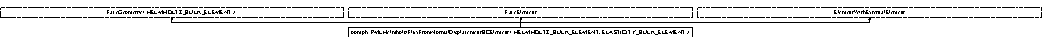
\includegraphics[height=0.492524cm]{classoomph_1_1PMLHelmholtzFluxFromNormalDisplacementBCElement}
\end{center}
\end{figure}
\subsection*{Public Member Functions}
\begin{DoxyCompactItemize}
\item 
\hyperlink{classoomph_1_1PMLHelmholtzFluxFromNormalDisplacementBCElement_abd57422005608f9ddfccefa73e6d757c}{P\+M\+L\+Helmholtz\+Flux\+From\+Normal\+Displacement\+B\+C\+Element} (Finite\+Element $\ast$const \&bulk\+\_\+el\+\_\+pt, const int \&face\+\_\+index)
\begin{DoxyCompactList}\small\item\em Constructor, takes the pointer to the \char`\"{}bulk\char`\"{} element and the face index identifying the face to which the element is attached. \end{DoxyCompactList}\item 
\hyperlink{classoomph_1_1PMLHelmholtzFluxFromNormalDisplacementBCElement_a4eaae55dc9bd4d6076cf9f6f75f06df3}{P\+M\+L\+Helmholtz\+Flux\+From\+Normal\+Displacement\+B\+C\+Element} (const \hyperlink{classoomph_1_1PMLHelmholtzFluxFromNormalDisplacementBCElement}{P\+M\+L\+Helmholtz\+Flux\+From\+Normal\+Displacement\+B\+C\+Element} \&dummy)
\begin{DoxyCompactList}\small\item\em Broken copy constructor. \end{DoxyCompactList}\item 
void \hyperlink{classoomph_1_1PMLHelmholtzFluxFromNormalDisplacementBCElement_ab43c2c8e318060cf808329b1c147a333}{fill\+\_\+in\+\_\+contribution\+\_\+to\+\_\+residuals} (Vector$<$ double $>$ \&residuals)
\begin{DoxyCompactList}\small\item\em Broken assignment operator. \end{DoxyCompactList}\item 
void \hyperlink{classoomph_1_1PMLHelmholtzFluxFromNormalDisplacementBCElement_a159c7c508fc565f7d70481cd467a5152}{fill\+\_\+in\+\_\+contribution\+\_\+to\+\_\+jacobian} (Vector$<$ double $>$ \&residuals, Dense\+Matrix$<$ double $>$ \&jacobian)
\begin{DoxyCompactList}\small\item\em Add the element\textquotesingle{}s contribution to its residual vector and its Jacobian matrix. \end{DoxyCompactList}\item 
void \hyperlink{classoomph_1_1PMLHelmholtzFluxFromNormalDisplacementBCElement_a64c0556634eed3070ae9a63d2a43efb5}{output} (std\+::ostream \&outfile)
\begin{DoxyCompactList}\small\item\em Output function. \end{DoxyCompactList}\item 
void \hyperlink{classoomph_1_1PMLHelmholtzFluxFromNormalDisplacementBCElement_af0317c3b22f661138ddc31968c67eed8}{output} (std\+::ostream \&outfile, const unsigned \&n\+\_\+plot)
\begin{DoxyCompactList}\small\item\em Output function\+: flux etc at Gauss points; n\+\_\+plot is ignored. \end{DoxyCompactList}\item 
void \hyperlink{classoomph_1_1PMLHelmholtzFluxFromNormalDisplacementBCElement_a357bf237c7b8a0d421851a6e8f93a9b6}{output} (F\+I\+LE $\ast$file\+\_\+pt)
\begin{DoxyCompactList}\small\item\em C-\/style output function. \end{DoxyCompactList}\item 
void \hyperlink{classoomph_1_1PMLHelmholtzFluxFromNormalDisplacementBCElement_a798feeb0c2f831476e3ded0a91c6a572}{output} (F\+I\+LE $\ast$file\+\_\+pt, const unsigned \&n\+\_\+plot)
\begin{DoxyCompactList}\small\item\em C-\/style output function. \end{DoxyCompactList}\end{DoxyCompactItemize}
\subsection*{Protected Member Functions}
\begin{DoxyCompactItemize}
\item 
double \hyperlink{classoomph_1_1PMLHelmholtzFluxFromNormalDisplacementBCElement_a4e6b686d2905fc642cb735d611830be4}{shape\+\_\+and\+\_\+test} (const Vector$<$ double $>$ \&s, Shape \&psi, Shape \&test) const
\begin{DoxyCompactList}\small\item\em Function to compute the shape and test functions and to return the Jacobian of mapping between local and global (Eulerian) coordinates. \end{DoxyCompactList}\item 
double \hyperlink{classoomph_1_1PMLHelmholtzFluxFromNormalDisplacementBCElement_ac0c13560b5e8dba19dc11f44f455bf97}{shape\+\_\+and\+\_\+test\+\_\+at\+\_\+knot} (const unsigned \&ipt, Shape \&psi, Shape \&test) const
\begin{DoxyCompactList}\small\item\em Function to compute the shape and test functions and to return. \end{DoxyCompactList}\end{DoxyCompactItemize}
\subsection*{Private Member Functions}
\begin{DoxyCompactItemize}
\item 
void \hyperlink{classoomph_1_1PMLHelmholtzFluxFromNormalDisplacementBCElement_a1efff41871abb12efe479ee7434b93b5}{fill\+\_\+in\+\_\+generic\+\_\+residual\+\_\+contribution\+\_\+helmholtz\+\_\+flux\+\_\+from\+\_\+displacement} (Vector$<$ double $>$ \&residuals, Dense\+Matrix$<$ double $>$ \&jacobian, const unsigned \&flag)
\begin{DoxyCompactList}\small\item\em Add the element\textquotesingle{}s contribution to its residual vector. flag=1(or 0)\+: do (or don\textquotesingle{}t) compute the contribution to the Jacobian as well. \end{DoxyCompactList}\end{DoxyCompactItemize}
\subsection*{Private Attributes}
\begin{DoxyCompactItemize}
\item 
unsigned \hyperlink{classoomph_1_1PMLHelmholtzFluxFromNormalDisplacementBCElement_a61904b123c934fd59b5c72f626ebb728}{Dim}
\begin{DoxyCompactList}\small\item\em The spatial dimension of the problem. \end{DoxyCompactList}\item 
std\+::complex$<$ unsigned $>$ \hyperlink{classoomph_1_1PMLHelmholtzFluxFromNormalDisplacementBCElement_aa80b2b79bd3c63f8d7c7f91d97fd22fc}{U\+\_\+index\+\_\+helmholtz\+\_\+from\+\_\+displacement}
\begin{DoxyCompactList}\small\item\em The index at which the unknown is stored at the nodes. \end{DoxyCompactList}\end{DoxyCompactItemize}


\subsection{Detailed Description}
\subsubsection*{template$<$class H\+E\+L\+M\+H\+O\+L\+T\+Z\+\_\+\+B\+U\+L\+K\+\_\+\+E\+L\+E\+M\+E\+NT, class E\+L\+A\+S\+T\+I\+C\+I\+T\+Y\+\_\+\+B\+U\+L\+K\+\_\+\+E\+L\+E\+M\+E\+NT$>$\newline
class oomph\+::\+P\+M\+L\+Helmholtz\+Flux\+From\+Normal\+Displacement\+B\+C\+Element$<$ H\+E\+L\+M\+H\+O\+L\+T\+Z\+\_\+\+B\+U\+L\+K\+\_\+\+E\+L\+E\+M\+E\+N\+T, E\+L\+A\+S\+T\+I\+C\+I\+T\+Y\+\_\+\+B\+U\+L\+K\+\_\+\+E\+L\+E\+M\+E\+N\+T $>$}

A class for elements that allow the imposition of an prescribed flux (determined from the normal displacements of an adjacent linearly elastic solid. Normal derivative for displacement potential is given by normal displacement of adjacent solid multiplies by F\+SI parameter (q = k$^\wedge$2 B/E). The element geometry is obtained from the Face\+Geometry$<$\+E\+L\+E\+M\+E\+N\+T$>$ policy class. 

Definition at line 698 of file pml\+\_\+helmholtz\+\_\+time\+\_\+harmonic\+\_\+linear\+\_\+elasticity\+\_\+interaction.\+h.



\subsection{Constructor \& Destructor Documentation}
\mbox{\Hypertarget{classoomph_1_1PMLHelmholtzFluxFromNormalDisplacementBCElement_abd57422005608f9ddfccefa73e6d757c}\label{classoomph_1_1PMLHelmholtzFluxFromNormalDisplacementBCElement_abd57422005608f9ddfccefa73e6d757c}} 
\index{oomph\+::\+P\+M\+L\+Helmholtz\+Flux\+From\+Normal\+Displacement\+B\+C\+Element@{oomph\+::\+P\+M\+L\+Helmholtz\+Flux\+From\+Normal\+Displacement\+B\+C\+Element}!P\+M\+L\+Helmholtz\+Flux\+From\+Normal\+Displacement\+B\+C\+Element@{P\+M\+L\+Helmholtz\+Flux\+From\+Normal\+Displacement\+B\+C\+Element}}
\index{P\+M\+L\+Helmholtz\+Flux\+From\+Normal\+Displacement\+B\+C\+Element@{P\+M\+L\+Helmholtz\+Flux\+From\+Normal\+Displacement\+B\+C\+Element}!oomph\+::\+P\+M\+L\+Helmholtz\+Flux\+From\+Normal\+Displacement\+B\+C\+Element@{oomph\+::\+P\+M\+L\+Helmholtz\+Flux\+From\+Normal\+Displacement\+B\+C\+Element}}
\subsubsection{\texorpdfstring{P\+M\+L\+Helmholtz\+Flux\+From\+Normal\+Displacement\+B\+C\+Element()}{PMLHelmholtzFluxFromNormalDisplacementBCElement()}\hspace{0.1cm}{\footnotesize\ttfamily [1/2]}}
{\footnotesize\ttfamily template$<$class H\+E\+L\+M\+H\+O\+L\+T\+Z\+\_\+\+B\+U\+L\+K\+\_\+\+E\+L\+E\+M\+E\+NT , class E\+L\+A\+S\+T\+I\+C\+I\+T\+Y\+\_\+\+B\+U\+L\+K\+\_\+\+E\+L\+E\+M\+E\+NT $>$ \\
\hyperlink{classoomph_1_1PMLHelmholtzFluxFromNormalDisplacementBCElement}{oomph\+::\+P\+M\+L\+Helmholtz\+Flux\+From\+Normal\+Displacement\+B\+C\+Element}$<$ H\+E\+L\+M\+H\+O\+L\+T\+Z\+\_\+\+B\+U\+L\+K\+\_\+\+E\+L\+E\+M\+E\+NT, E\+L\+A\+S\+T\+I\+C\+I\+T\+Y\+\_\+\+B\+U\+L\+K\+\_\+\+E\+L\+E\+M\+E\+NT $>$\+::\hyperlink{classoomph_1_1PMLHelmholtzFluxFromNormalDisplacementBCElement}{P\+M\+L\+Helmholtz\+Flux\+From\+Normal\+Displacement\+B\+C\+Element} (\begin{DoxyParamCaption}\item[{Finite\+Element $\ast$const \&}]{bulk\+\_\+el\+\_\+pt,  }\item[{const int \&}]{face\+\_\+index }\end{DoxyParamCaption})}



Constructor, takes the pointer to the \char`\"{}bulk\char`\"{} element and the face index identifying the face to which the element is attached. 

Constructor, takes the pointer to the \char`\"{}bulk\char`\"{} element, and the face index that identifies the face of the bulk element to which this face element is to be attached. 

Definition at line 917 of file pml\+\_\+helmholtz\+\_\+time\+\_\+harmonic\+\_\+linear\+\_\+elasticity\+\_\+interaction.\+h.



References oomph\+::\+P\+M\+L\+Helmholtz\+Flux\+From\+Normal\+Displacement\+B\+C\+Element$<$ H\+E\+L\+M\+H\+O\+L\+T\+Z\+\_\+\+B\+U\+L\+K\+\_\+\+E\+L\+E\+M\+E\+N\+T, E\+L\+A\+S\+T\+I\+C\+I\+T\+Y\+\_\+\+B\+U\+L\+K\+\_\+\+E\+L\+E\+M\+E\+N\+T $>$\+::\+Dim, oomph\+::\+P\+M\+L\+Helmholtz\+Flux\+From\+Normal\+Displacement\+B\+C\+Element$<$ H\+E\+L\+M\+H\+O\+L\+T\+Z\+\_\+\+B\+U\+L\+K\+\_\+\+E\+L\+E\+M\+E\+N\+T, E\+L\+A\+S\+T\+I\+C\+I\+T\+Y\+\_\+\+B\+U\+L\+K\+\_\+\+E\+L\+E\+M\+E\+N\+T $>$\+::fill\+\_\+in\+\_\+generic\+\_\+residual\+\_\+contribution\+\_\+helmholtz\+\_\+flux\+\_\+from\+\_\+displacement(), and oomph\+::\+P\+M\+L\+Helmholtz\+Flux\+From\+Normal\+Displacement\+B\+C\+Element$<$ H\+E\+L\+M\+H\+O\+L\+T\+Z\+\_\+\+B\+U\+L\+K\+\_\+\+E\+L\+E\+M\+E\+N\+T, E\+L\+A\+S\+T\+I\+C\+I\+T\+Y\+\_\+\+B\+U\+L\+K\+\_\+\+E\+L\+E\+M\+E\+N\+T $>$\+::\+U\+\_\+index\+\_\+helmholtz\+\_\+from\+\_\+displacement.

\mbox{\Hypertarget{classoomph_1_1PMLHelmholtzFluxFromNormalDisplacementBCElement_a4eaae55dc9bd4d6076cf9f6f75f06df3}\label{classoomph_1_1PMLHelmholtzFluxFromNormalDisplacementBCElement_a4eaae55dc9bd4d6076cf9f6f75f06df3}} 
\index{oomph\+::\+P\+M\+L\+Helmholtz\+Flux\+From\+Normal\+Displacement\+B\+C\+Element@{oomph\+::\+P\+M\+L\+Helmholtz\+Flux\+From\+Normal\+Displacement\+B\+C\+Element}!P\+M\+L\+Helmholtz\+Flux\+From\+Normal\+Displacement\+B\+C\+Element@{P\+M\+L\+Helmholtz\+Flux\+From\+Normal\+Displacement\+B\+C\+Element}}
\index{P\+M\+L\+Helmholtz\+Flux\+From\+Normal\+Displacement\+B\+C\+Element@{P\+M\+L\+Helmholtz\+Flux\+From\+Normal\+Displacement\+B\+C\+Element}!oomph\+::\+P\+M\+L\+Helmholtz\+Flux\+From\+Normal\+Displacement\+B\+C\+Element@{oomph\+::\+P\+M\+L\+Helmholtz\+Flux\+From\+Normal\+Displacement\+B\+C\+Element}}
\subsubsection{\texorpdfstring{P\+M\+L\+Helmholtz\+Flux\+From\+Normal\+Displacement\+B\+C\+Element()}{PMLHelmholtzFluxFromNormalDisplacementBCElement()}\hspace{0.1cm}{\footnotesize\ttfamily [2/2]}}
{\footnotesize\ttfamily template$<$class H\+E\+L\+M\+H\+O\+L\+T\+Z\+\_\+\+B\+U\+L\+K\+\_\+\+E\+L\+E\+M\+E\+NT , class E\+L\+A\+S\+T\+I\+C\+I\+T\+Y\+\_\+\+B\+U\+L\+K\+\_\+\+E\+L\+E\+M\+E\+NT $>$ \\
\hyperlink{classoomph_1_1PMLHelmholtzFluxFromNormalDisplacementBCElement}{oomph\+::\+P\+M\+L\+Helmholtz\+Flux\+From\+Normal\+Displacement\+B\+C\+Element}$<$ H\+E\+L\+M\+H\+O\+L\+T\+Z\+\_\+\+B\+U\+L\+K\+\_\+\+E\+L\+E\+M\+E\+NT, E\+L\+A\+S\+T\+I\+C\+I\+T\+Y\+\_\+\+B\+U\+L\+K\+\_\+\+E\+L\+E\+M\+E\+NT $>$\+::\hyperlink{classoomph_1_1PMLHelmholtzFluxFromNormalDisplacementBCElement}{P\+M\+L\+Helmholtz\+Flux\+From\+Normal\+Displacement\+B\+C\+Element} (\begin{DoxyParamCaption}\item[{const \hyperlink{classoomph_1_1PMLHelmholtzFluxFromNormalDisplacementBCElement}{P\+M\+L\+Helmholtz\+Flux\+From\+Normal\+Displacement\+B\+C\+Element}$<$ H\+E\+L\+M\+H\+O\+L\+T\+Z\+\_\+\+B\+U\+L\+K\+\_\+\+E\+L\+E\+M\+E\+NT, E\+L\+A\+S\+T\+I\+C\+I\+T\+Y\+\_\+\+B\+U\+L\+K\+\_\+\+E\+L\+E\+M\+E\+NT $>$ \&}]{dummy }\end{DoxyParamCaption})\hspace{0.3cm}{\ttfamily [inline]}}



Broken copy constructor. 



Definition at line 714 of file pml\+\_\+helmholtz\+\_\+time\+\_\+harmonic\+\_\+linear\+\_\+elasticity\+\_\+interaction.\+h.



\subsection{Member Function Documentation}
\mbox{\Hypertarget{classoomph_1_1PMLHelmholtzFluxFromNormalDisplacementBCElement_a159c7c508fc565f7d70481cd467a5152}\label{classoomph_1_1PMLHelmholtzFluxFromNormalDisplacementBCElement_a159c7c508fc565f7d70481cd467a5152}} 
\index{oomph\+::\+P\+M\+L\+Helmholtz\+Flux\+From\+Normal\+Displacement\+B\+C\+Element@{oomph\+::\+P\+M\+L\+Helmholtz\+Flux\+From\+Normal\+Displacement\+B\+C\+Element}!fill\+\_\+in\+\_\+contribution\+\_\+to\+\_\+jacobian@{fill\+\_\+in\+\_\+contribution\+\_\+to\+\_\+jacobian}}
\index{fill\+\_\+in\+\_\+contribution\+\_\+to\+\_\+jacobian@{fill\+\_\+in\+\_\+contribution\+\_\+to\+\_\+jacobian}!oomph\+::\+P\+M\+L\+Helmholtz\+Flux\+From\+Normal\+Displacement\+B\+C\+Element@{oomph\+::\+P\+M\+L\+Helmholtz\+Flux\+From\+Normal\+Displacement\+B\+C\+Element}}
\subsubsection{\texorpdfstring{fill\+\_\+in\+\_\+contribution\+\_\+to\+\_\+jacobian()}{fill\_in\_contribution\_to\_jacobian()}}
{\footnotesize\ttfamily template$<$class H\+E\+L\+M\+H\+O\+L\+T\+Z\+\_\+\+B\+U\+L\+K\+\_\+\+E\+L\+E\+M\+E\+NT , class E\+L\+A\+S\+T\+I\+C\+I\+T\+Y\+\_\+\+B\+U\+L\+K\+\_\+\+E\+L\+E\+M\+E\+NT $>$ \\
void \hyperlink{classoomph_1_1PMLHelmholtzFluxFromNormalDisplacementBCElement}{oomph\+::\+P\+M\+L\+Helmholtz\+Flux\+From\+Normal\+Displacement\+B\+C\+Element}$<$ H\+E\+L\+M\+H\+O\+L\+T\+Z\+\_\+\+B\+U\+L\+K\+\_\+\+E\+L\+E\+M\+E\+NT, E\+L\+A\+S\+T\+I\+C\+I\+T\+Y\+\_\+\+B\+U\+L\+K\+\_\+\+E\+L\+E\+M\+E\+NT $>$\+::fill\+\_\+in\+\_\+contribution\+\_\+to\+\_\+jacobian (\begin{DoxyParamCaption}\item[{Vector$<$ double $>$ \&}]{residuals,  }\item[{Dense\+Matrix$<$ double $>$ \&}]{jacobian }\end{DoxyParamCaption})\hspace{0.3cm}{\ttfamily [inline]}}



Add the element\textquotesingle{}s contribution to its residual vector and its Jacobian matrix. 



Definition at line 746 of file pml\+\_\+helmholtz\+\_\+time\+\_\+harmonic\+\_\+linear\+\_\+elasticity\+\_\+interaction.\+h.

\mbox{\Hypertarget{classoomph_1_1PMLHelmholtzFluxFromNormalDisplacementBCElement_ab43c2c8e318060cf808329b1c147a333}\label{classoomph_1_1PMLHelmholtzFluxFromNormalDisplacementBCElement_ab43c2c8e318060cf808329b1c147a333}} 
\index{oomph\+::\+P\+M\+L\+Helmholtz\+Flux\+From\+Normal\+Displacement\+B\+C\+Element@{oomph\+::\+P\+M\+L\+Helmholtz\+Flux\+From\+Normal\+Displacement\+B\+C\+Element}!fill\+\_\+in\+\_\+contribution\+\_\+to\+\_\+residuals@{fill\+\_\+in\+\_\+contribution\+\_\+to\+\_\+residuals}}
\index{fill\+\_\+in\+\_\+contribution\+\_\+to\+\_\+residuals@{fill\+\_\+in\+\_\+contribution\+\_\+to\+\_\+residuals}!oomph\+::\+P\+M\+L\+Helmholtz\+Flux\+From\+Normal\+Displacement\+B\+C\+Element@{oomph\+::\+P\+M\+L\+Helmholtz\+Flux\+From\+Normal\+Displacement\+B\+C\+Element}}
\subsubsection{\texorpdfstring{fill\+\_\+in\+\_\+contribution\+\_\+to\+\_\+residuals()}{fill\_in\_contribution\_to\_residuals()}}
{\footnotesize\ttfamily template$<$class H\+E\+L\+M\+H\+O\+L\+T\+Z\+\_\+\+B\+U\+L\+K\+\_\+\+E\+L\+E\+M\+E\+NT , class E\+L\+A\+S\+T\+I\+C\+I\+T\+Y\+\_\+\+B\+U\+L\+K\+\_\+\+E\+L\+E\+M\+E\+NT $>$ \\
void \hyperlink{classoomph_1_1PMLHelmholtzFluxFromNormalDisplacementBCElement}{oomph\+::\+P\+M\+L\+Helmholtz\+Flux\+From\+Normal\+Displacement\+B\+C\+Element}$<$ H\+E\+L\+M\+H\+O\+L\+T\+Z\+\_\+\+B\+U\+L\+K\+\_\+\+E\+L\+E\+M\+E\+NT, E\+L\+A\+S\+T\+I\+C\+I\+T\+Y\+\_\+\+B\+U\+L\+K\+\_\+\+E\+L\+E\+M\+E\+NT $>$\+::fill\+\_\+in\+\_\+contribution\+\_\+to\+\_\+residuals (\begin{DoxyParamCaption}\item[{Vector$<$ double $>$ \&}]{residuals }\end{DoxyParamCaption})\hspace{0.3cm}{\ttfamily [inline]}}



Broken assignment operator. 

Add the element\textquotesingle{}s contribution to its residual vector 

Definition at line 735 of file pml\+\_\+helmholtz\+\_\+time\+\_\+harmonic\+\_\+linear\+\_\+elasticity\+\_\+interaction.\+h.

\mbox{\Hypertarget{classoomph_1_1PMLHelmholtzFluxFromNormalDisplacementBCElement_a1efff41871abb12efe479ee7434b93b5}\label{classoomph_1_1PMLHelmholtzFluxFromNormalDisplacementBCElement_a1efff41871abb12efe479ee7434b93b5}} 
\index{oomph\+::\+P\+M\+L\+Helmholtz\+Flux\+From\+Normal\+Displacement\+B\+C\+Element@{oomph\+::\+P\+M\+L\+Helmholtz\+Flux\+From\+Normal\+Displacement\+B\+C\+Element}!fill\+\_\+in\+\_\+generic\+\_\+residual\+\_\+contribution\+\_\+helmholtz\+\_\+flux\+\_\+from\+\_\+displacement@{fill\+\_\+in\+\_\+generic\+\_\+residual\+\_\+contribution\+\_\+helmholtz\+\_\+flux\+\_\+from\+\_\+displacement}}
\index{fill\+\_\+in\+\_\+generic\+\_\+residual\+\_\+contribution\+\_\+helmholtz\+\_\+flux\+\_\+from\+\_\+displacement@{fill\+\_\+in\+\_\+generic\+\_\+residual\+\_\+contribution\+\_\+helmholtz\+\_\+flux\+\_\+from\+\_\+displacement}!oomph\+::\+P\+M\+L\+Helmholtz\+Flux\+From\+Normal\+Displacement\+B\+C\+Element@{oomph\+::\+P\+M\+L\+Helmholtz\+Flux\+From\+Normal\+Displacement\+B\+C\+Element}}
\subsubsection{\texorpdfstring{fill\+\_\+in\+\_\+generic\+\_\+residual\+\_\+contribution\+\_\+helmholtz\+\_\+flux\+\_\+from\+\_\+displacement()}{fill\_in\_generic\_residual\_contribution\_helmholtz\_flux\_from\_displacement()}}
{\footnotesize\ttfamily template$<$class H\+E\+L\+M\+H\+O\+L\+T\+Z\+\_\+\+B\+U\+L\+K\+\_\+\+E\+L\+E\+M\+E\+NT , class E\+L\+A\+S\+T\+I\+C\+I\+T\+Y\+\_\+\+B\+U\+L\+K\+\_\+\+E\+L\+E\+M\+E\+NT $>$ \\
void \hyperlink{classoomph_1_1PMLHelmholtzFluxFromNormalDisplacementBCElement}{oomph\+::\+P\+M\+L\+Helmholtz\+Flux\+From\+Normal\+Displacement\+B\+C\+Element}$<$ H\+E\+L\+M\+H\+O\+L\+T\+Z\+\_\+\+B\+U\+L\+K\+\_\+\+E\+L\+E\+M\+E\+NT, E\+L\+A\+S\+T\+I\+C\+I\+T\+Y\+\_\+\+B\+U\+L\+K\+\_\+\+E\+L\+E\+M\+E\+NT $>$\+::fill\+\_\+in\+\_\+generic\+\_\+residual\+\_\+contribution\+\_\+helmholtz\+\_\+flux\+\_\+from\+\_\+displacement (\begin{DoxyParamCaption}\item[{Vector$<$ double $>$ \&}]{residuals,  }\item[{Dense\+Matrix$<$ double $>$ \&}]{jacobian,  }\item[{const unsigned \&}]{flag }\end{DoxyParamCaption})\hspace{0.3cm}{\ttfamily [private]}}



Add the element\textquotesingle{}s contribution to its residual vector. flag=1(or 0)\+: do (or don\textquotesingle{}t) compute the contribution to the Jacobian as well. 

Helper function to compute the element\textquotesingle{}s residual vector and the Jacobian matrix. 

Definition at line 1085 of file pml\+\_\+helmholtz\+\_\+time\+\_\+harmonic\+\_\+linear\+\_\+elasticity\+\_\+interaction.\+h.



References oomph\+::\+P\+M\+L\+Helmholtz\+Flux\+From\+Normal\+Displacement\+B\+C\+Element$<$ H\+E\+L\+M\+H\+O\+L\+T\+Z\+\_\+\+B\+U\+L\+K\+\_\+\+E\+L\+E\+M\+E\+N\+T, E\+L\+A\+S\+T\+I\+C\+I\+T\+Y\+\_\+\+B\+U\+L\+K\+\_\+\+E\+L\+E\+M\+E\+N\+T $>$\+::\+Dim, oomph\+::\+P\+M\+L\+Helmholtz\+Flux\+From\+Normal\+Displacement\+B\+C\+Element$<$ H\+E\+L\+M\+H\+O\+L\+T\+Z\+\_\+\+B\+U\+L\+K\+\_\+\+E\+L\+E\+M\+E\+N\+T, E\+L\+A\+S\+T\+I\+C\+I\+T\+Y\+\_\+\+B\+U\+L\+K\+\_\+\+E\+L\+E\+M\+E\+N\+T $>$\+::shape\+\_\+and\+\_\+test(), and oomph\+::\+P\+M\+L\+Helmholtz\+Flux\+From\+Normal\+Displacement\+B\+C\+Element$<$ H\+E\+L\+M\+H\+O\+L\+T\+Z\+\_\+\+B\+U\+L\+K\+\_\+\+E\+L\+E\+M\+E\+N\+T, E\+L\+A\+S\+T\+I\+C\+I\+T\+Y\+\_\+\+B\+U\+L\+K\+\_\+\+E\+L\+E\+M\+E\+N\+T $>$\+::\+U\+\_\+index\+\_\+helmholtz\+\_\+from\+\_\+displacement.



Referenced by oomph\+::\+P\+M\+L\+Helmholtz\+Flux\+From\+Normal\+Displacement\+B\+C\+Element$<$ H\+E\+L\+M\+H\+O\+L\+T\+Z\+\_\+\+B\+U\+L\+K\+\_\+\+E\+L\+E\+M\+E\+N\+T, E\+L\+A\+S\+T\+I\+C\+I\+T\+Y\+\_\+\+B\+U\+L\+K\+\_\+\+E\+L\+E\+M\+E\+N\+T $>$\+::\+P\+M\+L\+Helmholtz\+Flux\+From\+Normal\+Displacement\+B\+C\+Element().

\mbox{\Hypertarget{classoomph_1_1PMLHelmholtzFluxFromNormalDisplacementBCElement_a64c0556634eed3070ae9a63d2a43efb5}\label{classoomph_1_1PMLHelmholtzFluxFromNormalDisplacementBCElement_a64c0556634eed3070ae9a63d2a43efb5}} 
\index{oomph\+::\+P\+M\+L\+Helmholtz\+Flux\+From\+Normal\+Displacement\+B\+C\+Element@{oomph\+::\+P\+M\+L\+Helmholtz\+Flux\+From\+Normal\+Displacement\+B\+C\+Element}!output@{output}}
\index{output@{output}!oomph\+::\+P\+M\+L\+Helmholtz\+Flux\+From\+Normal\+Displacement\+B\+C\+Element@{oomph\+::\+P\+M\+L\+Helmholtz\+Flux\+From\+Normal\+Displacement\+B\+C\+Element}}
\subsubsection{\texorpdfstring{output()}{output()}\hspace{0.1cm}{\footnotesize\ttfamily [1/4]}}
{\footnotesize\ttfamily template$<$class H\+E\+L\+M\+H\+O\+L\+T\+Z\+\_\+\+B\+U\+L\+K\+\_\+\+E\+L\+E\+M\+E\+NT , class E\+L\+A\+S\+T\+I\+C\+I\+T\+Y\+\_\+\+B\+U\+L\+K\+\_\+\+E\+L\+E\+M\+E\+NT $>$ \\
void \hyperlink{classoomph_1_1PMLHelmholtzFluxFromNormalDisplacementBCElement}{oomph\+::\+P\+M\+L\+Helmholtz\+Flux\+From\+Normal\+Displacement\+B\+C\+Element}$<$ H\+E\+L\+M\+H\+O\+L\+T\+Z\+\_\+\+B\+U\+L\+K\+\_\+\+E\+L\+E\+M\+E\+NT, E\+L\+A\+S\+T\+I\+C\+I\+T\+Y\+\_\+\+B\+U\+L\+K\+\_\+\+E\+L\+E\+M\+E\+NT $>$\+::output (\begin{DoxyParamCaption}\item[{std\+::ostream \&}]{outfile }\end{DoxyParamCaption})\hspace{0.3cm}{\ttfamily [inline]}}



Output function. 



Definition at line 758 of file pml\+\_\+helmholtz\+\_\+time\+\_\+harmonic\+\_\+linear\+\_\+elasticity\+\_\+interaction.\+h.



References oomph\+::\+Time\+Harmonic\+Lin\+Elast\+Loaded\+By\+P\+M\+L\+Helmholtz\+Pressure\+B\+C\+Element$<$ E\+L\+A\+S\+T\+I\+C\+I\+T\+Y\+\_\+\+B\+U\+L\+K\+\_\+\+E\+L\+E\+M\+E\+N\+T, H\+E\+L\+M\+H\+O\+L\+T\+Z\+\_\+\+B\+U\+L\+K\+\_\+\+E\+L\+E\+M\+E\+N\+T $>$\+::output().

\mbox{\Hypertarget{classoomph_1_1PMLHelmholtzFluxFromNormalDisplacementBCElement_af0317c3b22f661138ddc31968c67eed8}\label{classoomph_1_1PMLHelmholtzFluxFromNormalDisplacementBCElement_af0317c3b22f661138ddc31968c67eed8}} 
\index{oomph\+::\+P\+M\+L\+Helmholtz\+Flux\+From\+Normal\+Displacement\+B\+C\+Element@{oomph\+::\+P\+M\+L\+Helmholtz\+Flux\+From\+Normal\+Displacement\+B\+C\+Element}!output@{output}}
\index{output@{output}!oomph\+::\+P\+M\+L\+Helmholtz\+Flux\+From\+Normal\+Displacement\+B\+C\+Element@{oomph\+::\+P\+M\+L\+Helmholtz\+Flux\+From\+Normal\+Displacement\+B\+C\+Element}}
\subsubsection{\texorpdfstring{output()}{output()}\hspace{0.1cm}{\footnotesize\ttfamily [2/4]}}
{\footnotesize\ttfamily template$<$class H\+E\+L\+M\+H\+O\+L\+T\+Z\+\_\+\+B\+U\+L\+K\+\_\+\+E\+L\+E\+M\+E\+NT , class E\+L\+A\+S\+T\+I\+C\+I\+T\+Y\+\_\+\+B\+U\+L\+K\+\_\+\+E\+L\+E\+M\+E\+NT $>$ \\
void \hyperlink{classoomph_1_1PMLHelmholtzFluxFromNormalDisplacementBCElement}{oomph\+::\+P\+M\+L\+Helmholtz\+Flux\+From\+Normal\+Displacement\+B\+C\+Element}$<$ H\+E\+L\+M\+H\+O\+L\+T\+Z\+\_\+\+B\+U\+L\+K\+\_\+\+E\+L\+E\+M\+E\+NT, E\+L\+A\+S\+T\+I\+C\+I\+T\+Y\+\_\+\+B\+U\+L\+K\+\_\+\+E\+L\+E\+M\+E\+NT $>$\+::output (\begin{DoxyParamCaption}\item[{std\+::ostream \&}]{outfile,  }\item[{const unsigned \&}]{n\+\_\+plot }\end{DoxyParamCaption})\hspace{0.3cm}{\ttfamily [inline]}}



Output function\+: flux etc at Gauss points; n\+\_\+plot is ignored. 



Definition at line 766 of file pml\+\_\+helmholtz\+\_\+time\+\_\+harmonic\+\_\+linear\+\_\+elasticity\+\_\+interaction.\+h.

\mbox{\Hypertarget{classoomph_1_1PMLHelmholtzFluxFromNormalDisplacementBCElement_a357bf237c7b8a0d421851a6e8f93a9b6}\label{classoomph_1_1PMLHelmholtzFluxFromNormalDisplacementBCElement_a357bf237c7b8a0d421851a6e8f93a9b6}} 
\index{oomph\+::\+P\+M\+L\+Helmholtz\+Flux\+From\+Normal\+Displacement\+B\+C\+Element@{oomph\+::\+P\+M\+L\+Helmholtz\+Flux\+From\+Normal\+Displacement\+B\+C\+Element}!output@{output}}
\index{output@{output}!oomph\+::\+P\+M\+L\+Helmholtz\+Flux\+From\+Normal\+Displacement\+B\+C\+Element@{oomph\+::\+P\+M\+L\+Helmholtz\+Flux\+From\+Normal\+Displacement\+B\+C\+Element}}
\subsubsection{\texorpdfstring{output()}{output()}\hspace{0.1cm}{\footnotesize\ttfamily [3/4]}}
{\footnotesize\ttfamily template$<$class H\+E\+L\+M\+H\+O\+L\+T\+Z\+\_\+\+B\+U\+L\+K\+\_\+\+E\+L\+E\+M\+E\+NT , class E\+L\+A\+S\+T\+I\+C\+I\+T\+Y\+\_\+\+B\+U\+L\+K\+\_\+\+E\+L\+E\+M\+E\+NT $>$ \\
void \hyperlink{classoomph_1_1PMLHelmholtzFluxFromNormalDisplacementBCElement}{oomph\+::\+P\+M\+L\+Helmholtz\+Flux\+From\+Normal\+Displacement\+B\+C\+Element}$<$ H\+E\+L\+M\+H\+O\+L\+T\+Z\+\_\+\+B\+U\+L\+K\+\_\+\+E\+L\+E\+M\+E\+NT, E\+L\+A\+S\+T\+I\+C\+I\+T\+Y\+\_\+\+B\+U\+L\+K\+\_\+\+E\+L\+E\+M\+E\+NT $>$\+::output (\begin{DoxyParamCaption}\item[{F\+I\+LE $\ast$}]{file\+\_\+pt }\end{DoxyParamCaption})\hspace{0.3cm}{\ttfamily [inline]}}



C-\/style output function. 



Definition at line 830 of file pml\+\_\+helmholtz\+\_\+time\+\_\+harmonic\+\_\+linear\+\_\+elasticity\+\_\+interaction.\+h.

\mbox{\Hypertarget{classoomph_1_1PMLHelmholtzFluxFromNormalDisplacementBCElement_a798feeb0c2f831476e3ded0a91c6a572}\label{classoomph_1_1PMLHelmholtzFluxFromNormalDisplacementBCElement_a798feeb0c2f831476e3ded0a91c6a572}} 
\index{oomph\+::\+P\+M\+L\+Helmholtz\+Flux\+From\+Normal\+Displacement\+B\+C\+Element@{oomph\+::\+P\+M\+L\+Helmholtz\+Flux\+From\+Normal\+Displacement\+B\+C\+Element}!output@{output}}
\index{output@{output}!oomph\+::\+P\+M\+L\+Helmholtz\+Flux\+From\+Normal\+Displacement\+B\+C\+Element@{oomph\+::\+P\+M\+L\+Helmholtz\+Flux\+From\+Normal\+Displacement\+B\+C\+Element}}
\subsubsection{\texorpdfstring{output()}{output()}\hspace{0.1cm}{\footnotesize\ttfamily [4/4]}}
{\footnotesize\ttfamily template$<$class H\+E\+L\+M\+H\+O\+L\+T\+Z\+\_\+\+B\+U\+L\+K\+\_\+\+E\+L\+E\+M\+E\+NT , class E\+L\+A\+S\+T\+I\+C\+I\+T\+Y\+\_\+\+B\+U\+L\+K\+\_\+\+E\+L\+E\+M\+E\+NT $>$ \\
void \hyperlink{classoomph_1_1PMLHelmholtzFluxFromNormalDisplacementBCElement}{oomph\+::\+P\+M\+L\+Helmholtz\+Flux\+From\+Normal\+Displacement\+B\+C\+Element}$<$ H\+E\+L\+M\+H\+O\+L\+T\+Z\+\_\+\+B\+U\+L\+K\+\_\+\+E\+L\+E\+M\+E\+NT, E\+L\+A\+S\+T\+I\+C\+I\+T\+Y\+\_\+\+B\+U\+L\+K\+\_\+\+E\+L\+E\+M\+E\+NT $>$\+::output (\begin{DoxyParamCaption}\item[{F\+I\+LE $\ast$}]{file\+\_\+pt,  }\item[{const unsigned \&}]{n\+\_\+plot }\end{DoxyParamCaption})\hspace{0.3cm}{\ttfamily [inline]}}



C-\/style output function. 



Definition at line 834 of file pml\+\_\+helmholtz\+\_\+time\+\_\+harmonic\+\_\+linear\+\_\+elasticity\+\_\+interaction.\+h.

\mbox{\Hypertarget{classoomph_1_1PMLHelmholtzFluxFromNormalDisplacementBCElement_a4e6b686d2905fc642cb735d611830be4}\label{classoomph_1_1PMLHelmholtzFluxFromNormalDisplacementBCElement_a4e6b686d2905fc642cb735d611830be4}} 
\index{oomph\+::\+P\+M\+L\+Helmholtz\+Flux\+From\+Normal\+Displacement\+B\+C\+Element@{oomph\+::\+P\+M\+L\+Helmholtz\+Flux\+From\+Normal\+Displacement\+B\+C\+Element}!shape\+\_\+and\+\_\+test@{shape\+\_\+and\+\_\+test}}
\index{shape\+\_\+and\+\_\+test@{shape\+\_\+and\+\_\+test}!oomph\+::\+P\+M\+L\+Helmholtz\+Flux\+From\+Normal\+Displacement\+B\+C\+Element@{oomph\+::\+P\+M\+L\+Helmholtz\+Flux\+From\+Normal\+Displacement\+B\+C\+Element}}
\subsubsection{\texorpdfstring{shape\+\_\+and\+\_\+test()}{shape\_and\_test()}}
{\footnotesize\ttfamily template$<$class H\+E\+L\+M\+H\+O\+L\+T\+Z\+\_\+\+B\+U\+L\+K\+\_\+\+E\+L\+E\+M\+E\+NT , class E\+L\+A\+S\+T\+I\+C\+I\+T\+Y\+\_\+\+B\+U\+L\+K\+\_\+\+E\+L\+E\+M\+E\+NT $>$ \\
double \hyperlink{classoomph_1_1PMLHelmholtzFluxFromNormalDisplacementBCElement}{oomph\+::\+P\+M\+L\+Helmholtz\+Flux\+From\+Normal\+Displacement\+B\+C\+Element}$<$ H\+E\+L\+M\+H\+O\+L\+T\+Z\+\_\+\+B\+U\+L\+K\+\_\+\+E\+L\+E\+M\+E\+NT, E\+L\+A\+S\+T\+I\+C\+I\+T\+Y\+\_\+\+B\+U\+L\+K\+\_\+\+E\+L\+E\+M\+E\+NT $>$\+::shape\+\_\+and\+\_\+test (\begin{DoxyParamCaption}\item[{const Vector$<$ double $>$ \&}]{s,  }\item[{Shape \&}]{psi,  }\item[{Shape \&}]{test }\end{DoxyParamCaption}) const\hspace{0.3cm}{\ttfamily [inline]}, {\ttfamily [protected]}}



Function to compute the shape and test functions and to return the Jacobian of mapping between local and global (Eulerian) coordinates. 



Definition at line 844 of file pml\+\_\+helmholtz\+\_\+time\+\_\+harmonic\+\_\+linear\+\_\+elasticity\+\_\+interaction.\+h.



Referenced by oomph\+::\+P\+M\+L\+Helmholtz\+Flux\+From\+Normal\+Displacement\+B\+C\+Element$<$ H\+E\+L\+M\+H\+O\+L\+T\+Z\+\_\+\+B\+U\+L\+K\+\_\+\+E\+L\+E\+M\+E\+N\+T, E\+L\+A\+S\+T\+I\+C\+I\+T\+Y\+\_\+\+B\+U\+L\+K\+\_\+\+E\+L\+E\+M\+E\+N\+T $>$\+::fill\+\_\+in\+\_\+generic\+\_\+residual\+\_\+contribution\+\_\+helmholtz\+\_\+flux\+\_\+from\+\_\+displacement().

\mbox{\Hypertarget{classoomph_1_1PMLHelmholtzFluxFromNormalDisplacementBCElement_ac0c13560b5e8dba19dc11f44f455bf97}\label{classoomph_1_1PMLHelmholtzFluxFromNormalDisplacementBCElement_ac0c13560b5e8dba19dc11f44f455bf97}} 
\index{oomph\+::\+P\+M\+L\+Helmholtz\+Flux\+From\+Normal\+Displacement\+B\+C\+Element@{oomph\+::\+P\+M\+L\+Helmholtz\+Flux\+From\+Normal\+Displacement\+B\+C\+Element}!shape\+\_\+and\+\_\+test\+\_\+at\+\_\+knot@{shape\+\_\+and\+\_\+test\+\_\+at\+\_\+knot}}
\index{shape\+\_\+and\+\_\+test\+\_\+at\+\_\+knot@{shape\+\_\+and\+\_\+test\+\_\+at\+\_\+knot}!oomph\+::\+P\+M\+L\+Helmholtz\+Flux\+From\+Normal\+Displacement\+B\+C\+Element@{oomph\+::\+P\+M\+L\+Helmholtz\+Flux\+From\+Normal\+Displacement\+B\+C\+Element}}
\subsubsection{\texorpdfstring{shape\+\_\+and\+\_\+test\+\_\+at\+\_\+knot()}{shape\_and\_test\_at\_knot()}}
{\footnotesize\ttfamily template$<$class H\+E\+L\+M\+H\+O\+L\+T\+Z\+\_\+\+B\+U\+L\+K\+\_\+\+E\+L\+E\+M\+E\+NT , class E\+L\+A\+S\+T\+I\+C\+I\+T\+Y\+\_\+\+B\+U\+L\+K\+\_\+\+E\+L\+E\+M\+E\+NT $>$ \\
double \hyperlink{classoomph_1_1PMLHelmholtzFluxFromNormalDisplacementBCElement}{oomph\+::\+P\+M\+L\+Helmholtz\+Flux\+From\+Normal\+Displacement\+B\+C\+Element}$<$ H\+E\+L\+M\+H\+O\+L\+T\+Z\+\_\+\+B\+U\+L\+K\+\_\+\+E\+L\+E\+M\+E\+NT, E\+L\+A\+S\+T\+I\+C\+I\+T\+Y\+\_\+\+B\+U\+L\+K\+\_\+\+E\+L\+E\+M\+E\+NT $>$\+::shape\+\_\+and\+\_\+test\+\_\+at\+\_\+knot (\begin{DoxyParamCaption}\item[{const unsigned \&}]{ipt,  }\item[{Shape \&}]{psi,  }\item[{Shape \&}]{test }\end{DoxyParamCaption}) const\hspace{0.3cm}{\ttfamily [inline]}, {\ttfamily [protected]}}



Function to compute the shape and test functions and to return. 

the Jacobian of mapping between local and global (Eulerian) coordinates 

Definition at line 865 of file pml\+\_\+helmholtz\+\_\+time\+\_\+harmonic\+\_\+linear\+\_\+elasticity\+\_\+interaction.\+h.



\subsection{Member Data Documentation}
\mbox{\Hypertarget{classoomph_1_1PMLHelmholtzFluxFromNormalDisplacementBCElement_a61904b123c934fd59b5c72f626ebb728}\label{classoomph_1_1PMLHelmholtzFluxFromNormalDisplacementBCElement_a61904b123c934fd59b5c72f626ebb728}} 
\index{oomph\+::\+P\+M\+L\+Helmholtz\+Flux\+From\+Normal\+Displacement\+B\+C\+Element@{oomph\+::\+P\+M\+L\+Helmholtz\+Flux\+From\+Normal\+Displacement\+B\+C\+Element}!Dim@{Dim}}
\index{Dim@{Dim}!oomph\+::\+P\+M\+L\+Helmholtz\+Flux\+From\+Normal\+Displacement\+B\+C\+Element@{oomph\+::\+P\+M\+L\+Helmholtz\+Flux\+From\+Normal\+Displacement\+B\+C\+Element}}
\subsubsection{\texorpdfstring{Dim}{Dim}}
{\footnotesize\ttfamily template$<$class H\+E\+L\+M\+H\+O\+L\+T\+Z\+\_\+\+B\+U\+L\+K\+\_\+\+E\+L\+E\+M\+E\+NT , class E\+L\+A\+S\+T\+I\+C\+I\+T\+Y\+\_\+\+B\+U\+L\+K\+\_\+\+E\+L\+E\+M\+E\+NT $>$ \\
unsigned \hyperlink{classoomph_1_1PMLHelmholtzFluxFromNormalDisplacementBCElement}{oomph\+::\+P\+M\+L\+Helmholtz\+Flux\+From\+Normal\+Displacement\+B\+C\+Element}$<$ H\+E\+L\+M\+H\+O\+L\+T\+Z\+\_\+\+B\+U\+L\+K\+\_\+\+E\+L\+E\+M\+E\+NT, E\+L\+A\+S\+T\+I\+C\+I\+T\+Y\+\_\+\+B\+U\+L\+K\+\_\+\+E\+L\+E\+M\+E\+NT $>$\+::Dim\hspace{0.3cm}{\ttfamily [private]}}



The spatial dimension of the problem. 



Definition at line 895 of file pml\+\_\+helmholtz\+\_\+time\+\_\+harmonic\+\_\+linear\+\_\+elasticity\+\_\+interaction.\+h.



Referenced by oomph\+::\+P\+M\+L\+Helmholtz\+Flux\+From\+Normal\+Displacement\+B\+C\+Element$<$ H\+E\+L\+M\+H\+O\+L\+T\+Z\+\_\+\+B\+U\+L\+K\+\_\+\+E\+L\+E\+M\+E\+N\+T, E\+L\+A\+S\+T\+I\+C\+I\+T\+Y\+\_\+\+B\+U\+L\+K\+\_\+\+E\+L\+E\+M\+E\+N\+T $>$\+::fill\+\_\+in\+\_\+generic\+\_\+residual\+\_\+contribution\+\_\+helmholtz\+\_\+flux\+\_\+from\+\_\+displacement(), and oomph\+::\+P\+M\+L\+Helmholtz\+Flux\+From\+Normal\+Displacement\+B\+C\+Element$<$ H\+E\+L\+M\+H\+O\+L\+T\+Z\+\_\+\+B\+U\+L\+K\+\_\+\+E\+L\+E\+M\+E\+N\+T, E\+L\+A\+S\+T\+I\+C\+I\+T\+Y\+\_\+\+B\+U\+L\+K\+\_\+\+E\+L\+E\+M\+E\+N\+T $>$\+::\+P\+M\+L\+Helmholtz\+Flux\+From\+Normal\+Displacement\+B\+C\+Element().

\mbox{\Hypertarget{classoomph_1_1PMLHelmholtzFluxFromNormalDisplacementBCElement_aa80b2b79bd3c63f8d7c7f91d97fd22fc}\label{classoomph_1_1PMLHelmholtzFluxFromNormalDisplacementBCElement_aa80b2b79bd3c63f8d7c7f91d97fd22fc}} 
\index{oomph\+::\+P\+M\+L\+Helmholtz\+Flux\+From\+Normal\+Displacement\+B\+C\+Element@{oomph\+::\+P\+M\+L\+Helmholtz\+Flux\+From\+Normal\+Displacement\+B\+C\+Element}!U\+\_\+index\+\_\+helmholtz\+\_\+from\+\_\+displacement@{U\+\_\+index\+\_\+helmholtz\+\_\+from\+\_\+displacement}}
\index{U\+\_\+index\+\_\+helmholtz\+\_\+from\+\_\+displacement@{U\+\_\+index\+\_\+helmholtz\+\_\+from\+\_\+displacement}!oomph\+::\+P\+M\+L\+Helmholtz\+Flux\+From\+Normal\+Displacement\+B\+C\+Element@{oomph\+::\+P\+M\+L\+Helmholtz\+Flux\+From\+Normal\+Displacement\+B\+C\+Element}}
\subsubsection{\texorpdfstring{U\+\_\+index\+\_\+helmholtz\+\_\+from\+\_\+displacement}{U\_index\_helmholtz\_from\_displacement}}
{\footnotesize\ttfamily template$<$class H\+E\+L\+M\+H\+O\+L\+T\+Z\+\_\+\+B\+U\+L\+K\+\_\+\+E\+L\+E\+M\+E\+NT , class E\+L\+A\+S\+T\+I\+C\+I\+T\+Y\+\_\+\+B\+U\+L\+K\+\_\+\+E\+L\+E\+M\+E\+NT $>$ \\
std\+::complex$<$unsigned$>$ \hyperlink{classoomph_1_1PMLHelmholtzFluxFromNormalDisplacementBCElement}{oomph\+::\+P\+M\+L\+Helmholtz\+Flux\+From\+Normal\+Displacement\+B\+C\+Element}$<$ H\+E\+L\+M\+H\+O\+L\+T\+Z\+\_\+\+B\+U\+L\+K\+\_\+\+E\+L\+E\+M\+E\+NT, E\+L\+A\+S\+T\+I\+C\+I\+T\+Y\+\_\+\+B\+U\+L\+K\+\_\+\+E\+L\+E\+M\+E\+NT $>$\+::U\+\_\+index\+\_\+helmholtz\+\_\+from\+\_\+displacement\hspace{0.3cm}{\ttfamily [private]}}



The index at which the unknown is stored at the nodes. 



Definition at line 898 of file pml\+\_\+helmholtz\+\_\+time\+\_\+harmonic\+\_\+linear\+\_\+elasticity\+\_\+interaction.\+h.



Referenced by oomph\+::\+P\+M\+L\+Helmholtz\+Flux\+From\+Normal\+Displacement\+B\+C\+Element$<$ H\+E\+L\+M\+H\+O\+L\+T\+Z\+\_\+\+B\+U\+L\+K\+\_\+\+E\+L\+E\+M\+E\+N\+T, E\+L\+A\+S\+T\+I\+C\+I\+T\+Y\+\_\+\+B\+U\+L\+K\+\_\+\+E\+L\+E\+M\+E\+N\+T $>$\+::fill\+\_\+in\+\_\+generic\+\_\+residual\+\_\+contribution\+\_\+helmholtz\+\_\+flux\+\_\+from\+\_\+displacement(), and oomph\+::\+P\+M\+L\+Helmholtz\+Flux\+From\+Normal\+Displacement\+B\+C\+Element$<$ H\+E\+L\+M\+H\+O\+L\+T\+Z\+\_\+\+B\+U\+L\+K\+\_\+\+E\+L\+E\+M\+E\+N\+T, E\+L\+A\+S\+T\+I\+C\+I\+T\+Y\+\_\+\+B\+U\+L\+K\+\_\+\+E\+L\+E\+M\+E\+N\+T $>$\+::\+P\+M\+L\+Helmholtz\+Flux\+From\+Normal\+Displacement\+B\+C\+Element().



The documentation for this class was generated from the following file\+:\begin{DoxyCompactItemize}
\item 
\hyperlink{pml__helmholtz__time__harmonic__linear__elasticity__interaction_8h}{pml\+\_\+helmholtz\+\_\+time\+\_\+harmonic\+\_\+linear\+\_\+elasticity\+\_\+interaction.\+h}\end{DoxyCompactItemize}

\hypertarget{classoomph_1_1PseudoElasticFSIPreconditioner}{}\section{oomph\+:\+:Pseudo\+Elastic\+F\+S\+I\+Preconditioner Class Reference}
\label{classoomph_1_1PseudoElasticFSIPreconditioner}\index{oomph\+::\+Pseudo\+Elastic\+F\+S\+I\+Preconditioner@{oomph\+::\+Pseudo\+Elastic\+F\+S\+I\+Preconditioner}}


\hyperlink{classoomph_1_1Preconditioner}{Preconditioner} for F\+SI problems with pseudo-\/elastic fluid node updates. Note\+: \hyperlink{classoomph_1_1NavierStokesSchurComplementPreconditioner}{Navier\+Stokes\+Schur\+Complement\+Preconditioner} is applied to the Navier Stokes subsidiary system. Default solid preconditioner is \hyperlink{classoomph_1_1SuperLUPreconditioner}{Super\+L\+U\+Preconditioner}. {\bfseries Enumeration} of Elastic D\+OF types in the Pseudo-\/\+Elastic Elements The method get\+\_\+dof\+\_\+types\+\_\+for\+\_\+unknowns() must be implemented such that D\+O\+Fs subject be Lagrange multiplier and D\+O\+Fs N\+OT subject to Lagrange multiplier have different labels. For example in a 3D problem there are 6 D\+OF types and the following labelling must be implemented\+: 0 -\/ x displacement (without lagr mult traction) 1 -\/ y displacement (without lagr mult traction) 2 -\/ z displacement (without lagr mult traction) 3 -\/ x displacement (with lagr mult traction) 4 -\/ y displacement (with lagr mult traction) 5 -\/ z displacement (with lagr mult traction)  




{\ttfamily \#include $<$pseudo\+\_\+elastic\+\_\+fsi\+\_\+preconditioner.\+h$>$}

Inheritance diagram for oomph\+:\+:Pseudo\+Elastic\+F\+S\+I\+Preconditioner\+:\begin{figure}[H]
\begin{center}
\leavevmode
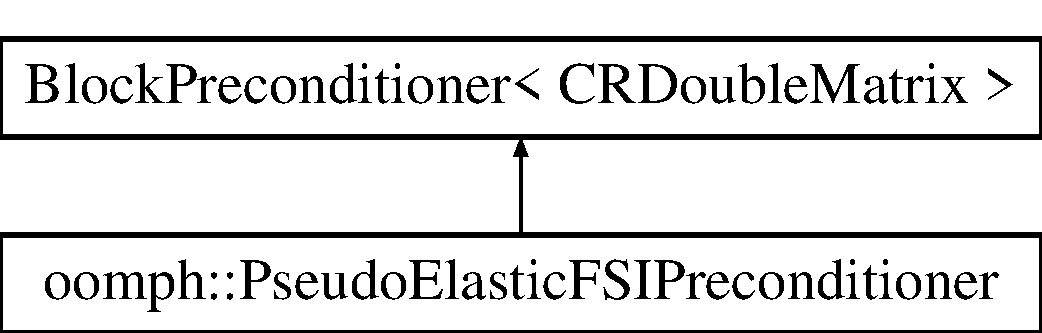
\includegraphics[height=4.000000cm]{classoomph_1_1PseudoElasticFSIPreconditioner}
\end{center}
\end{figure}
\subsection*{Public Member Functions}
\begin{DoxyCompactItemize}
\item 
\hyperlink{classoomph_1_1PseudoElasticFSIPreconditioner_aa3132ef3e4ecd57adf64da72e84b5d9d}{Pseudo\+Elastic\+F\+S\+I\+Preconditioner} (const unsigned \&dim, \hyperlink{classoomph_1_1Problem}{Problem} $\ast$problem\+\_\+pt)
\begin{DoxyCompactList}\small\item\em constructor -\/ just set defaults. Specify the spatial dimension of the fluid and a (non-\/const) problem pointer needed for the underlying \hyperlink{classoomph_1_1NavierStokesSchurComplementPreconditioner}{Navier\+Stokes\+Schur\+Complement\+Preconditioner}. \end{DoxyCompactList}\item 
virtual \hyperlink{classoomph_1_1PseudoElasticFSIPreconditioner_a8f57b2dc7f9e37d419ead6b786dfac82}{$\sim$\+Pseudo\+Elastic\+F\+S\+I\+Preconditioner} ()
\item 
\hyperlink{classoomph_1_1PseudoElasticFSIPreconditioner_aa7efe57119bf77e503049922f8d16722}{Pseudo\+Elastic\+F\+S\+I\+Preconditioner} (const \hyperlink{classoomph_1_1PseudoElasticFSIPreconditioner}{Pseudo\+Elastic\+F\+S\+I\+Preconditioner} \&)
\begin{DoxyCompactList}\small\item\em Broken copy constructor. \end{DoxyCompactList}\item 
void \hyperlink{classoomph_1_1PseudoElasticFSIPreconditioner_a15859381010faa40a47fdca28b281475}{clean\+\_\+up\+\_\+memory} ()
\begin{DoxyCompactList}\small\item\em Broken assignment operator. \end{DoxyCompactList}\item 
void \hyperlink{classoomph_1_1PseudoElasticFSIPreconditioner_a460ad5eea59f4c07dfde8b11696fabb1}{setup} ()
\begin{DoxyCompactList}\small\item\em Setup the precoonditioner. \end{DoxyCompactList}\item 
void \hyperlink{classoomph_1_1PseudoElasticFSIPreconditioner_ad29c2852949caec2d20cbe7cf99f1b38}{preconditioner\+\_\+solve} (const \hyperlink{classoomph_1_1DoubleVector}{Double\+Vector} \&r, \hyperlink{classoomph_1_1DoubleVector}{Double\+Vector} \&z)
\begin{DoxyCompactList}\small\item\em Apply the preconditioner. \end{DoxyCompactList}\item 
void \hyperlink{classoomph_1_1PseudoElasticFSIPreconditioner_a8d0b7212ad06c4f5942fed253c680010}{set\+\_\+fluid\+\_\+and\+\_\+pseudo\+\_\+elastic\+\_\+mesh\+\_\+pt} (\hyperlink{classoomph_1_1Mesh}{Mesh} $\ast$\hyperlink{classoomph_1_1BlockPreconditioner_a3c0e92cb77c3e3179007fe9fd99b6428}{mesh\+\_\+pt})
\begin{DoxyCompactList}\small\item\em specify the mesh containing the combined fluid/pseudo solid elements \end{DoxyCompactList}\item 
void \hyperlink{classoomph_1_1PseudoElasticFSIPreconditioner_af2c1fc8d2dd795c5a4a2ae266ad32d18}{set\+\_\+solid\+\_\+mesh\+\_\+pt} (\hyperlink{classoomph_1_1Mesh}{Mesh} $\ast$\hyperlink{classoomph_1_1BlockPreconditioner_a3c0e92cb77c3e3179007fe9fd99b6428}{mesh\+\_\+pt})
\begin{DoxyCompactList}\small\item\em specify the mesh containing the solid elements \end{DoxyCompactList}\item 
void \hyperlink{classoomph_1_1PseudoElasticFSIPreconditioner_ad30185179d7c2bc6c725e550c48a0c90}{set\+\_\+lagrange\+\_\+multiplier\+\_\+mesh\+\_\+pt} (\hyperlink{classoomph_1_1Mesh}{Mesh} $\ast$\hyperlink{classoomph_1_1BlockPreconditioner_a3c0e92cb77c3e3179007fe9fd99b6428}{mesh\+\_\+pt})
\begin{DoxyCompactList}\small\item\em specify the mesh containing the lagrange multiplier elements \end{DoxyCompactList}\item 
void \hyperlink{classoomph_1_1PseudoElasticFSIPreconditioner_a92e59f83606d77e7407a4ace534546f2}{set\+\_\+solid\+\_\+preconditioner} (\hyperlink{classoomph_1_1Preconditioner}{Preconditioner} $\ast$prec\+\_\+pt)
\begin{DoxyCompactList}\small\item\em speicify a non default solid preconditioner. This preconditioner will not delete it \end{DoxyCompactList}\item 
\hyperlink{classoomph_1_1PseudoElasticPreconditioner}{Pseudo\+Elastic\+Preconditioner} $\ast$const \hyperlink{classoomph_1_1PseudoElasticFSIPreconditioner_af10b20ad8e90cd99ba35326f1207d6a7}{pseudo\+\_\+elastic\+\_\+preconditioner\+\_\+pt} ()
\begin{DoxyCompactList}\small\item\em Access function to the pseudo elastic subsidiary preconditioner. \end{DoxyCompactList}\item 
\hyperlink{classoomph_1_1NavierStokesSchurComplementPreconditioner}{Navier\+Stokes\+Schur\+Complement\+Preconditioner} $\ast$const \hyperlink{classoomph_1_1PseudoElasticFSIPreconditioner_a4e13b64643e9026f421fa1228333ca95}{navier\+\_\+stokes\+\_\+schur\+\_\+complement\+\_\+preconditioner\+\_\+pt} ()
\begin{DoxyCompactList}\small\item\em Access function to the Navier Stokes Schur complement preconditioner. \end{DoxyCompactList}\item 
void \hyperlink{classoomph_1_1PseudoElasticFSIPreconditioner_a136fa015ebb39a20e82682bacd65c65b}{enable\+\_\+navier\+\_\+stokes\+\_\+schur\+\_\+complement\+\_\+preconditioner} ()
\begin{DoxyCompactList}\small\item\em Call to use the Navier Stokes Schur complement preconditioner. \end{DoxyCompactList}\item 
void \hyperlink{classoomph_1_1PseudoElasticFSIPreconditioner_af2adaec06d407d4b89bca034984c66ba}{disable\+\_\+navier\+\_\+stokes\+\_\+schur\+\_\+complement\+\_\+preconditioner} ()
\begin{DoxyCompactList}\small\item\em Call to use the \hyperlink{classoomph_1_1SuperLUPreconditioner}{Super\+L\+U\+Preconditioner} is used for the Navier Stokes subsidiary system. \end{DoxyCompactList}\end{DoxyCompactItemize}
\subsection*{Private Attributes}
\begin{DoxyCompactItemize}
\item 
\hyperlink{classoomph_1_1PseudoElasticPreconditioner}{Pseudo\+Elastic\+Preconditioner} $\ast$ \hyperlink{classoomph_1_1PseudoElasticFSIPreconditioner_afad4b204e6b7b2a63e4c4e0fe2f9f2c0}{Pseudo\+\_\+elastic\+\_\+preconditioner\+\_\+pt}
\begin{DoxyCompactList}\small\item\em pointer to the pseudo solid preconditioner \end{DoxyCompactList}\item 
\hyperlink{classoomph_1_1Preconditioner}{Preconditioner} $\ast$ \hyperlink{classoomph_1_1PseudoElasticFSIPreconditioner_a5314b4734298c3de8f394a45792ba1c9}{Navier\+\_\+stokes\+\_\+preconditioner\+\_\+pt}
\begin{DoxyCompactList}\small\item\em pointer to the navier stokes precondtioner \end{DoxyCompactList}\item 
\hyperlink{classoomph_1_1NavierStokesSchurComplementPreconditioner}{Navier\+Stokes\+Schur\+Complement\+Preconditioner} $\ast$ \hyperlink{classoomph_1_1PseudoElasticFSIPreconditioner_a438b2a5932c1fde633a73107043f0b09}{Navier\+\_\+stokes\+\_\+schur\+\_\+complement\+\_\+preconditioner\+\_\+pt}
\begin{DoxyCompactList}\small\item\em Navier Stokes Schur complement preconditioner. \end{DoxyCompactList}\item 
\hyperlink{classoomph_1_1Preconditioner}{Preconditioner} $\ast$ \hyperlink{classoomph_1_1PseudoElasticFSIPreconditioner_a2d96e724939038637ff4911372ee69b4}{Solid\+\_\+preconditioner\+\_\+pt}
\begin{DoxyCompactList}\small\item\em pointer to the solid preconditioner \end{DoxyCompactList}\item 
bool \hyperlink{classoomph_1_1PseudoElasticFSIPreconditioner_aab116f252418ca092f7e6f0f75de6778}{Using\+\_\+default\+\_\+solid\+\_\+preconditioner}
\begin{DoxyCompactList}\small\item\em boolean flag to indicate whether default Solid preconditioner is used \end{DoxyCompactList}\item 
bool \hyperlink{classoomph_1_1PseudoElasticFSIPreconditioner_aa58001a8248ecac64087de254c0ae763}{Solid\+\_\+preconditioner\+\_\+is\+\_\+block\+\_\+preconditioner}
\begin{DoxyCompactList}\small\item\em boolean flag to indicate whether the Solid preconditioner is a block preconditioner \end{DoxyCompactList}\item 
\hyperlink{classoomph_1_1MatrixVectorProduct}{Matrix\+Vector\+Product} $\ast$ \hyperlink{classoomph_1_1PseudoElasticFSIPreconditioner_a77c8b262ee8535947e52f36462544eec}{Fluid\+\_\+pseudo\+\_\+elastic\+\_\+matvec\+\_\+pt}
\begin{DoxyCompactList}\small\item\em fluid onto pseudosolid matrix vector operator \end{DoxyCompactList}\item 
\hyperlink{classoomph_1_1MatrixVectorProduct}{Matrix\+Vector\+Product} $\ast$ \hyperlink{classoomph_1_1PseudoElasticFSIPreconditioner_a8699afc5b64ec0c3db5c3cea5fd60c18}{Solid\+\_\+fluid\+\_\+matvec\+\_\+pt}
\begin{DoxyCompactList}\small\item\em solid onto fluid matrix vector operatio \end{DoxyCompactList}\item 
\hyperlink{classoomph_1_1MatrixVectorProduct}{Matrix\+Vector\+Product} $\ast$ \hyperlink{classoomph_1_1PseudoElasticFSIPreconditioner_a05eb73f45602a85e5dfb0a9cd10a488e}{Solid\+\_\+pseudo\+\_\+elastic\+\_\+matvec\+\_\+pt}
\begin{DoxyCompactList}\small\item\em solid onto pseudo solid matrix vector operatio \end{DoxyCompactList}\item 
\hyperlink{classoomph_1_1MatrixVectorProduct}{Matrix\+Vector\+Product} $\ast$ \hyperlink{classoomph_1_1PseudoElasticFSIPreconditioner_a1129dcb6e7e335aca44acdb4231adc38}{Lagrange\+\_\+solid\+\_\+matvec\+\_\+pt}
\item 
\hyperlink{classoomph_1_1Mesh}{Mesh} $\ast$ \hyperlink{classoomph_1_1PseudoElasticFSIPreconditioner_a9d8025b022a2ca180210da2f7979dfe2}{Fluid\+\_\+and\+\_\+pseudo\+\_\+elastic\+\_\+mesh\+\_\+pt}
\begin{DoxyCompactList}\small\item\em \hyperlink{classoomph_1_1Mesh}{Mesh} containing the combined fluid and pseudo solid element. \end{DoxyCompactList}\item 
\hyperlink{classoomph_1_1Mesh}{Mesh} $\ast$ \hyperlink{classoomph_1_1PseudoElasticFSIPreconditioner_afd02372d56906a9f86c5b00bf50297aa}{Solid\+\_\+mesh\+\_\+pt}
\begin{DoxyCompactList}\small\item\em \hyperlink{classoomph_1_1Mesh}{Mesh} containing the solid elements. \end{DoxyCompactList}\item 
\hyperlink{classoomph_1_1Mesh}{Mesh} $\ast$ \hyperlink{classoomph_1_1PseudoElasticFSIPreconditioner_a0a75413264015a10ce59e7a31c7fe7c4}{Lagrange\+\_\+multiplier\+\_\+mesh\+\_\+pt}
\begin{DoxyCompactList}\small\item\em \hyperlink{classoomph_1_1Mesh}{Mesh} containing the lagrange multiplier elements. \end{DoxyCompactList}\item 
unsigned \hyperlink{classoomph_1_1PseudoElasticFSIPreconditioner_aec1e28a3a746a76ed6a283115e8d3146}{Dim}
\begin{DoxyCompactList}\small\item\em the dimension of the fluid \end{DoxyCompactList}\item 
bool \hyperlink{classoomph_1_1PseudoElasticFSIPreconditioner_aa9eab77e9d4dfbdecfac9cccceb68c7b}{Use\+\_\+navier\+\_\+stokes\+\_\+schur\+\_\+complement\+\_\+preconditioner}
\begin{DoxyCompactList}\small\item\em If true the Navier Stokes Schur complement preconditioner is used. Otherwise \hyperlink{classoomph_1_1SuperLUPreconditioner}{Super\+L\+U\+Preconditioner} is used for the Navier Stokes subsidiary system. \end{DoxyCompactList}\end{DoxyCompactItemize}
\subsection*{Additional Inherited Members}


\subsection{Detailed Description}
\hyperlink{classoomph_1_1Preconditioner}{Preconditioner} for F\+SI problems with pseudo-\/elastic fluid node updates. Note\+: \hyperlink{classoomph_1_1NavierStokesSchurComplementPreconditioner}{Navier\+Stokes\+Schur\+Complement\+Preconditioner} is applied to the Navier Stokes subsidiary system. Default solid preconditioner is \hyperlink{classoomph_1_1SuperLUPreconditioner}{Super\+L\+U\+Preconditioner}. {\bfseries Enumeration} of Elastic D\+OF types in the Pseudo-\/\+Elastic Elements The method get\+\_\+dof\+\_\+types\+\_\+for\+\_\+unknowns() must be implemented such that D\+O\+Fs subject be Lagrange multiplier and D\+O\+Fs N\+OT subject to Lagrange multiplier have different labels. For example in a 3D problem there are 6 D\+OF types and the following labelling must be implemented\+: 0 -\/ x displacement (without lagr mult traction) 1 -\/ y displacement (without lagr mult traction) 2 -\/ z displacement (without lagr mult traction) 3 -\/ x displacement (with lagr mult traction) 4 -\/ y displacement (with lagr mult traction) 5 -\/ z displacement (with lagr mult traction) 

Definition at line 64 of file pseudo\+\_\+elastic\+\_\+fsi\+\_\+preconditioner.\+h.



\subsection{Constructor \& Destructor Documentation}
\mbox{\Hypertarget{classoomph_1_1PseudoElasticFSIPreconditioner_aa3132ef3e4ecd57adf64da72e84b5d9d}\label{classoomph_1_1PseudoElasticFSIPreconditioner_aa3132ef3e4ecd57adf64da72e84b5d9d}} 
\index{oomph\+::\+Pseudo\+Elastic\+F\+S\+I\+Preconditioner@{oomph\+::\+Pseudo\+Elastic\+F\+S\+I\+Preconditioner}!Pseudo\+Elastic\+F\+S\+I\+Preconditioner@{Pseudo\+Elastic\+F\+S\+I\+Preconditioner}}
\index{Pseudo\+Elastic\+F\+S\+I\+Preconditioner@{Pseudo\+Elastic\+F\+S\+I\+Preconditioner}!oomph\+::\+Pseudo\+Elastic\+F\+S\+I\+Preconditioner@{oomph\+::\+Pseudo\+Elastic\+F\+S\+I\+Preconditioner}}
\subsubsection{\texorpdfstring{Pseudo\+Elastic\+F\+S\+I\+Preconditioner()}{PseudoElasticFSIPreconditioner()}\hspace{0.1cm}{\footnotesize\ttfamily [1/2]}}
{\footnotesize\ttfamily oomph\+::\+Pseudo\+Elastic\+F\+S\+I\+Preconditioner\+::\+Pseudo\+Elastic\+F\+S\+I\+Preconditioner (\begin{DoxyParamCaption}\item[{const unsigned \&}]{dim,  }\item[{\hyperlink{classoomph_1_1Problem}{Problem} $\ast$}]{problem\+\_\+pt }\end{DoxyParamCaption})\hspace{0.3cm}{\ttfamily [inline]}}



constructor -\/ just set defaults. Specify the spatial dimension of the fluid and a (non-\/const) problem pointer needed for the underlying \hyperlink{classoomph_1_1NavierStokesSchurComplementPreconditioner}{Navier\+Stokes\+Schur\+Complement\+Preconditioner}. 



Definition at line 73 of file pseudo\+\_\+elastic\+\_\+fsi\+\_\+preconditioner.\+h.



References Fluid\+\_\+and\+\_\+pseudo\+\_\+elastic\+\_\+mesh\+\_\+pt, Fluid\+\_\+pseudo\+\_\+elastic\+\_\+matvec\+\_\+pt, Lagrange\+\_\+multiplier\+\_\+mesh\+\_\+pt, Lagrange\+\_\+solid\+\_\+matvec\+\_\+pt, Navier\+\_\+stokes\+\_\+preconditioner\+\_\+pt, Navier\+\_\+stokes\+\_\+schur\+\_\+complement\+\_\+preconditioner\+\_\+pt, Pseudo\+\_\+elastic\+\_\+preconditioner\+\_\+pt, oomph\+::\+Block\+Preconditioner$<$ C\+R\+Double\+Matrix $>$\+::set\+\_\+nmesh(), Solid\+\_\+fluid\+\_\+matvec\+\_\+pt, Solid\+\_\+mesh\+\_\+pt, Solid\+\_\+preconditioner\+\_\+pt, Solid\+\_\+pseudo\+\_\+elastic\+\_\+matvec\+\_\+pt, Use\+\_\+navier\+\_\+stokes\+\_\+schur\+\_\+complement\+\_\+preconditioner, and Using\+\_\+default\+\_\+solid\+\_\+preconditioner.

\mbox{\Hypertarget{classoomph_1_1PseudoElasticFSIPreconditioner_a8f57b2dc7f9e37d419ead6b786dfac82}\label{classoomph_1_1PseudoElasticFSIPreconditioner_a8f57b2dc7f9e37d419ead6b786dfac82}} 
\index{oomph\+::\+Pseudo\+Elastic\+F\+S\+I\+Preconditioner@{oomph\+::\+Pseudo\+Elastic\+F\+S\+I\+Preconditioner}!````~Pseudo\+Elastic\+F\+S\+I\+Preconditioner@{$\sim$\+Pseudo\+Elastic\+F\+S\+I\+Preconditioner}}
\index{````~Pseudo\+Elastic\+F\+S\+I\+Preconditioner@{$\sim$\+Pseudo\+Elastic\+F\+S\+I\+Preconditioner}!oomph\+::\+Pseudo\+Elastic\+F\+S\+I\+Preconditioner@{oomph\+::\+Pseudo\+Elastic\+F\+S\+I\+Preconditioner}}
\subsubsection{\texorpdfstring{$\sim$\+Pseudo\+Elastic\+F\+S\+I\+Preconditioner()}{~PseudoElasticFSIPreconditioner()}}
{\footnotesize\ttfamily virtual oomph\+::\+Pseudo\+Elastic\+F\+S\+I\+Preconditioner\+::$\sim$\+Pseudo\+Elastic\+F\+S\+I\+Preconditioner (\begin{DoxyParamCaption}{ }\end{DoxyParamCaption})\hspace{0.3cm}{\ttfamily [inline]}, {\ttfamily [virtual]}}



Definition at line 109 of file pseudo\+\_\+elastic\+\_\+fsi\+\_\+preconditioner.\+h.



References clean\+\_\+up\+\_\+memory(), Fluid\+\_\+pseudo\+\_\+elastic\+\_\+matvec\+\_\+pt, Lagrange\+\_\+solid\+\_\+matvec\+\_\+pt, Navier\+\_\+stokes\+\_\+preconditioner\+\_\+pt, Navier\+\_\+stokes\+\_\+schur\+\_\+complement\+\_\+preconditioner\+\_\+pt, Pseudo\+\_\+elastic\+\_\+preconditioner\+\_\+pt, Solid\+\_\+fluid\+\_\+matvec\+\_\+pt, Solid\+\_\+preconditioner\+\_\+pt, Solid\+\_\+pseudo\+\_\+elastic\+\_\+matvec\+\_\+pt, and Using\+\_\+default\+\_\+solid\+\_\+preconditioner.

\mbox{\Hypertarget{classoomph_1_1PseudoElasticFSIPreconditioner_aa7efe57119bf77e503049922f8d16722}\label{classoomph_1_1PseudoElasticFSIPreconditioner_aa7efe57119bf77e503049922f8d16722}} 
\index{oomph\+::\+Pseudo\+Elastic\+F\+S\+I\+Preconditioner@{oomph\+::\+Pseudo\+Elastic\+F\+S\+I\+Preconditioner}!Pseudo\+Elastic\+F\+S\+I\+Preconditioner@{Pseudo\+Elastic\+F\+S\+I\+Preconditioner}}
\index{Pseudo\+Elastic\+F\+S\+I\+Preconditioner@{Pseudo\+Elastic\+F\+S\+I\+Preconditioner}!oomph\+::\+Pseudo\+Elastic\+F\+S\+I\+Preconditioner@{oomph\+::\+Pseudo\+Elastic\+F\+S\+I\+Preconditioner}}
\subsubsection{\texorpdfstring{Pseudo\+Elastic\+F\+S\+I\+Preconditioner()}{PseudoElasticFSIPreconditioner()}\hspace{0.1cm}{\footnotesize\ttfamily [2/2]}}
{\footnotesize\ttfamily oomph\+::\+Pseudo\+Elastic\+F\+S\+I\+Preconditioner\+::\+Pseudo\+Elastic\+F\+S\+I\+Preconditioner (\begin{DoxyParamCaption}\item[{const \hyperlink{classoomph_1_1PseudoElasticFSIPreconditioner}{Pseudo\+Elastic\+F\+S\+I\+Preconditioner} \&}]{ }\end{DoxyParamCaption})\hspace{0.3cm}{\ttfamily [inline]}}



Broken copy constructor. 



Definition at line 135 of file pseudo\+\_\+elastic\+\_\+fsi\+\_\+preconditioner.\+h.



References oomph\+::\+Broken\+Copy\+::broken\+\_\+copy(), clean\+\_\+up\+\_\+memory(), preconditioner\+\_\+solve(), and setup().



\subsection{Member Function Documentation}
\mbox{\Hypertarget{classoomph_1_1PseudoElasticFSIPreconditioner_a15859381010faa40a47fdca28b281475}\label{classoomph_1_1PseudoElasticFSIPreconditioner_a15859381010faa40a47fdca28b281475}} 
\index{oomph\+::\+Pseudo\+Elastic\+F\+S\+I\+Preconditioner@{oomph\+::\+Pseudo\+Elastic\+F\+S\+I\+Preconditioner}!clean\+\_\+up\+\_\+memory@{clean\+\_\+up\+\_\+memory}}
\index{clean\+\_\+up\+\_\+memory@{clean\+\_\+up\+\_\+memory}!oomph\+::\+Pseudo\+Elastic\+F\+S\+I\+Preconditioner@{oomph\+::\+Pseudo\+Elastic\+F\+S\+I\+Preconditioner}}
\subsubsection{\texorpdfstring{clean\+\_\+up\+\_\+memory()}{clean\_up\_memory()}}
{\footnotesize\ttfamily void oomph\+::\+Pseudo\+Elastic\+F\+S\+I\+Preconditioner\+::clean\+\_\+up\+\_\+memory (\begin{DoxyParamCaption}{ }\end{DoxyParamCaption})\hspace{0.3cm}{\ttfamily [virtual]}}



Broken assignment operator. 

clean up memory method 

Reimplemented from \hyperlink{classoomph_1_1Preconditioner_a46c31c416829bedcd9db238431262027}{oomph\+::\+Preconditioner}.



Definition at line 38 of file pseudo\+\_\+elastic\+\_\+fsi\+\_\+preconditioner.\+cc.



References oomph\+::\+Matrix\+Vector\+Product\+::clean\+\_\+up\+\_\+memory(), oomph\+::\+Preconditioner\+::clean\+\_\+up\+\_\+memory(), oomph\+::\+Pseudo\+Elastic\+Preconditioner\+::clean\+\_\+up\+\_\+memory(), oomph\+::\+Navier\+Stokes\+Schur\+Complement\+Preconditioner\+::clean\+\_\+up\+\_\+memory(), Fluid\+\_\+pseudo\+\_\+elastic\+\_\+matvec\+\_\+pt, Lagrange\+\_\+solid\+\_\+matvec\+\_\+pt, Navier\+\_\+stokes\+\_\+preconditioner\+\_\+pt, Navier\+\_\+stokes\+\_\+schur\+\_\+complement\+\_\+preconditioner\+\_\+pt, Pseudo\+\_\+elastic\+\_\+preconditioner\+\_\+pt, Solid\+\_\+fluid\+\_\+matvec\+\_\+pt, Solid\+\_\+preconditioner\+\_\+pt, and Solid\+\_\+pseudo\+\_\+elastic\+\_\+matvec\+\_\+pt.



Referenced by Pseudo\+Elastic\+F\+S\+I\+Preconditioner(), setup(), and $\sim$\+Pseudo\+Elastic\+F\+S\+I\+Preconditioner().

\mbox{\Hypertarget{classoomph_1_1PseudoElasticFSIPreconditioner_af2adaec06d407d4b89bca034984c66ba}\label{classoomph_1_1PseudoElasticFSIPreconditioner_af2adaec06d407d4b89bca034984c66ba}} 
\index{oomph\+::\+Pseudo\+Elastic\+F\+S\+I\+Preconditioner@{oomph\+::\+Pseudo\+Elastic\+F\+S\+I\+Preconditioner}!disable\+\_\+navier\+\_\+stokes\+\_\+schur\+\_\+complement\+\_\+preconditioner@{disable\+\_\+navier\+\_\+stokes\+\_\+schur\+\_\+complement\+\_\+preconditioner}}
\index{disable\+\_\+navier\+\_\+stokes\+\_\+schur\+\_\+complement\+\_\+preconditioner@{disable\+\_\+navier\+\_\+stokes\+\_\+schur\+\_\+complement\+\_\+preconditioner}!oomph\+::\+Pseudo\+Elastic\+F\+S\+I\+Preconditioner@{oomph\+::\+Pseudo\+Elastic\+F\+S\+I\+Preconditioner}}
\subsubsection{\texorpdfstring{disable\+\_\+navier\+\_\+stokes\+\_\+schur\+\_\+complement\+\_\+preconditioner()}{disable\_navier\_stokes\_schur\_complement\_preconditioner()}}
{\footnotesize\ttfamily void oomph\+::\+Pseudo\+Elastic\+F\+S\+I\+Preconditioner\+::disable\+\_\+navier\+\_\+stokes\+\_\+schur\+\_\+complement\+\_\+preconditioner (\begin{DoxyParamCaption}{ }\end{DoxyParamCaption})\hspace{0.3cm}{\ttfamily [inline]}}



Call to use the \hyperlink{classoomph_1_1SuperLUPreconditioner}{Super\+L\+U\+Preconditioner} is used for the Navier Stokes subsidiary system. 



Definition at line 211 of file pseudo\+\_\+elastic\+\_\+fsi\+\_\+preconditioner.\+h.



References Use\+\_\+navier\+\_\+stokes\+\_\+schur\+\_\+complement\+\_\+preconditioner.

\mbox{\Hypertarget{classoomph_1_1PseudoElasticFSIPreconditioner_a136fa015ebb39a20e82682bacd65c65b}\label{classoomph_1_1PseudoElasticFSIPreconditioner_a136fa015ebb39a20e82682bacd65c65b}} 
\index{oomph\+::\+Pseudo\+Elastic\+F\+S\+I\+Preconditioner@{oomph\+::\+Pseudo\+Elastic\+F\+S\+I\+Preconditioner}!enable\+\_\+navier\+\_\+stokes\+\_\+schur\+\_\+complement\+\_\+preconditioner@{enable\+\_\+navier\+\_\+stokes\+\_\+schur\+\_\+complement\+\_\+preconditioner}}
\index{enable\+\_\+navier\+\_\+stokes\+\_\+schur\+\_\+complement\+\_\+preconditioner@{enable\+\_\+navier\+\_\+stokes\+\_\+schur\+\_\+complement\+\_\+preconditioner}!oomph\+::\+Pseudo\+Elastic\+F\+S\+I\+Preconditioner@{oomph\+::\+Pseudo\+Elastic\+F\+S\+I\+Preconditioner}}
\subsubsection{\texorpdfstring{enable\+\_\+navier\+\_\+stokes\+\_\+schur\+\_\+complement\+\_\+preconditioner()}{enable\_navier\_stokes\_schur\_complement\_preconditioner()}}
{\footnotesize\ttfamily void oomph\+::\+Pseudo\+Elastic\+F\+S\+I\+Preconditioner\+::enable\+\_\+navier\+\_\+stokes\+\_\+schur\+\_\+complement\+\_\+preconditioner (\begin{DoxyParamCaption}{ }\end{DoxyParamCaption})\hspace{0.3cm}{\ttfamily [inline]}}



Call to use the Navier Stokes Schur complement preconditioner. 



Definition at line 206 of file pseudo\+\_\+elastic\+\_\+fsi\+\_\+preconditioner.\+h.



References Use\+\_\+navier\+\_\+stokes\+\_\+schur\+\_\+complement\+\_\+preconditioner.

\mbox{\Hypertarget{classoomph_1_1PseudoElasticFSIPreconditioner_a4e13b64643e9026f421fa1228333ca95}\label{classoomph_1_1PseudoElasticFSIPreconditioner_a4e13b64643e9026f421fa1228333ca95}} 
\index{oomph\+::\+Pseudo\+Elastic\+F\+S\+I\+Preconditioner@{oomph\+::\+Pseudo\+Elastic\+F\+S\+I\+Preconditioner}!navier\+\_\+stokes\+\_\+schur\+\_\+complement\+\_\+preconditioner\+\_\+pt@{navier\+\_\+stokes\+\_\+schur\+\_\+complement\+\_\+preconditioner\+\_\+pt}}
\index{navier\+\_\+stokes\+\_\+schur\+\_\+complement\+\_\+preconditioner\+\_\+pt@{navier\+\_\+stokes\+\_\+schur\+\_\+complement\+\_\+preconditioner\+\_\+pt}!oomph\+::\+Pseudo\+Elastic\+F\+S\+I\+Preconditioner@{oomph\+::\+Pseudo\+Elastic\+F\+S\+I\+Preconditioner}}
\subsubsection{\texorpdfstring{navier\+\_\+stokes\+\_\+schur\+\_\+complement\+\_\+preconditioner\+\_\+pt()}{navier\_stokes\_schur\_complement\_preconditioner\_pt()}}
{\footnotesize\ttfamily \hyperlink{classoomph_1_1NavierStokesSchurComplementPreconditioner}{Navier\+Stokes\+Schur\+Complement\+Preconditioner}$\ast$ const oomph\+::\+Pseudo\+Elastic\+F\+S\+I\+Preconditioner\+::navier\+\_\+stokes\+\_\+schur\+\_\+complement\+\_\+preconditioner\+\_\+pt (\begin{DoxyParamCaption}{ }\end{DoxyParamCaption})\hspace{0.3cm}{\ttfamily [inline]}}



Access function to the Navier Stokes Schur complement preconditioner. 



Definition at line 199 of file pseudo\+\_\+elastic\+\_\+fsi\+\_\+preconditioner.\+h.



References Navier\+\_\+stokes\+\_\+schur\+\_\+complement\+\_\+preconditioner\+\_\+pt.

\mbox{\Hypertarget{classoomph_1_1PseudoElasticFSIPreconditioner_ad29c2852949caec2d20cbe7cf99f1b38}\label{classoomph_1_1PseudoElasticFSIPreconditioner_ad29c2852949caec2d20cbe7cf99f1b38}} 
\index{oomph\+::\+Pseudo\+Elastic\+F\+S\+I\+Preconditioner@{oomph\+::\+Pseudo\+Elastic\+F\+S\+I\+Preconditioner}!preconditioner\+\_\+solve@{preconditioner\+\_\+solve}}
\index{preconditioner\+\_\+solve@{preconditioner\+\_\+solve}!oomph\+::\+Pseudo\+Elastic\+F\+S\+I\+Preconditioner@{oomph\+::\+Pseudo\+Elastic\+F\+S\+I\+Preconditioner}}
\subsubsection{\texorpdfstring{preconditioner\+\_\+solve()}{preconditioner\_solve()}}
{\footnotesize\ttfamily void oomph\+::\+Pseudo\+Elastic\+F\+S\+I\+Preconditioner\+::preconditioner\+\_\+solve (\begin{DoxyParamCaption}\item[{const \hyperlink{classoomph_1_1DoubleVector}{Double\+Vector} \&}]{r,  }\item[{\hyperlink{classoomph_1_1DoubleVector}{Double\+Vector} \&}]{z }\end{DoxyParamCaption})\hspace{0.3cm}{\ttfamily [virtual]}}



Apply the preconditioner. 



Implements \hyperlink{classoomph_1_1Preconditioner_ace1199369e4465cd2b9a34884bb64ec8}{oomph\+::\+Preconditioner}.



Definition at line 286 of file pseudo\+\_\+elastic\+\_\+fsi\+\_\+preconditioner.\+cc.



References oomph\+::\+Double\+Vector\+::build(), oomph\+::\+Double\+Vector\+::clear(), oomph\+::\+Pseudo\+Elastic\+Preconditioner\+::elastic\+\_\+preconditioner\+\_\+solve(), Fluid\+\_\+pseudo\+\_\+elastic\+\_\+matvec\+\_\+pt, oomph\+::\+Block\+Preconditioner$<$ C\+R\+Double\+Matrix $>$\+::get\+\_\+block\+\_\+vector(), Lagrange\+\_\+solid\+\_\+matvec\+\_\+pt, oomph\+::\+Matrix\+Vector\+Product\+::multiply(), Navier\+\_\+stokes\+\_\+preconditioner\+\_\+pt, Navier\+\_\+stokes\+\_\+schur\+\_\+complement\+\_\+preconditioner\+\_\+pt, oomph\+::\+Preconditioner\+::preconditioner\+\_\+solve(), Pseudo\+\_\+elastic\+\_\+preconditioner\+\_\+pt, oomph\+::\+Block\+Preconditioner$<$ C\+R\+Double\+Matrix $>$\+::return\+\_\+block\+\_\+vector(), Solid\+\_\+fluid\+\_\+matvec\+\_\+pt, Solid\+\_\+preconditioner\+\_\+is\+\_\+block\+\_\+preconditioner, Solid\+\_\+preconditioner\+\_\+pt, Solid\+\_\+pseudo\+\_\+elastic\+\_\+matvec\+\_\+pt, and Use\+\_\+navier\+\_\+stokes\+\_\+schur\+\_\+complement\+\_\+preconditioner.



Referenced by Pseudo\+Elastic\+F\+S\+I\+Preconditioner(), and setup().

\mbox{\Hypertarget{classoomph_1_1PseudoElasticFSIPreconditioner_af10b20ad8e90cd99ba35326f1207d6a7}\label{classoomph_1_1PseudoElasticFSIPreconditioner_af10b20ad8e90cd99ba35326f1207d6a7}} 
\index{oomph\+::\+Pseudo\+Elastic\+F\+S\+I\+Preconditioner@{oomph\+::\+Pseudo\+Elastic\+F\+S\+I\+Preconditioner}!pseudo\+\_\+elastic\+\_\+preconditioner\+\_\+pt@{pseudo\+\_\+elastic\+\_\+preconditioner\+\_\+pt}}
\index{pseudo\+\_\+elastic\+\_\+preconditioner\+\_\+pt@{pseudo\+\_\+elastic\+\_\+preconditioner\+\_\+pt}!oomph\+::\+Pseudo\+Elastic\+F\+S\+I\+Preconditioner@{oomph\+::\+Pseudo\+Elastic\+F\+S\+I\+Preconditioner}}
\subsubsection{\texorpdfstring{pseudo\+\_\+elastic\+\_\+preconditioner\+\_\+pt()}{pseudo\_elastic\_preconditioner\_pt()}}
{\footnotesize\ttfamily \hyperlink{classoomph_1_1PseudoElasticPreconditioner}{Pseudo\+Elastic\+Preconditioner}$\ast$ const oomph\+::\+Pseudo\+Elastic\+F\+S\+I\+Preconditioner\+::pseudo\+\_\+elastic\+\_\+preconditioner\+\_\+pt (\begin{DoxyParamCaption}{ }\end{DoxyParamCaption})\hspace{0.3cm}{\ttfamily [inline]}}



Access function to the pseudo elastic subsidiary preconditioner. 



Definition at line 192 of file pseudo\+\_\+elastic\+\_\+fsi\+\_\+preconditioner.\+h.



References Pseudo\+\_\+elastic\+\_\+preconditioner\+\_\+pt.

\mbox{\Hypertarget{classoomph_1_1PseudoElasticFSIPreconditioner_a8d0b7212ad06c4f5942fed253c680010}\label{classoomph_1_1PseudoElasticFSIPreconditioner_a8d0b7212ad06c4f5942fed253c680010}} 
\index{oomph\+::\+Pseudo\+Elastic\+F\+S\+I\+Preconditioner@{oomph\+::\+Pseudo\+Elastic\+F\+S\+I\+Preconditioner}!set\+\_\+fluid\+\_\+and\+\_\+pseudo\+\_\+elastic\+\_\+mesh\+\_\+pt@{set\+\_\+fluid\+\_\+and\+\_\+pseudo\+\_\+elastic\+\_\+mesh\+\_\+pt}}
\index{set\+\_\+fluid\+\_\+and\+\_\+pseudo\+\_\+elastic\+\_\+mesh\+\_\+pt@{set\+\_\+fluid\+\_\+and\+\_\+pseudo\+\_\+elastic\+\_\+mesh\+\_\+pt}!oomph\+::\+Pseudo\+Elastic\+F\+S\+I\+Preconditioner@{oomph\+::\+Pseudo\+Elastic\+F\+S\+I\+Preconditioner}}
\subsubsection{\texorpdfstring{set\+\_\+fluid\+\_\+and\+\_\+pseudo\+\_\+elastic\+\_\+mesh\+\_\+pt()}{set\_fluid\_and\_pseudo\_elastic\_mesh\_pt()}}
{\footnotesize\ttfamily void oomph\+::\+Pseudo\+Elastic\+F\+S\+I\+Preconditioner\+::set\+\_\+fluid\+\_\+and\+\_\+pseudo\+\_\+elastic\+\_\+mesh\+\_\+pt (\begin{DoxyParamCaption}\item[{\hyperlink{classoomph_1_1Mesh}{Mesh} $\ast$}]{mesh\+\_\+pt }\end{DoxyParamCaption})\hspace{0.3cm}{\ttfamily [inline]}}



specify the mesh containing the combined fluid/pseudo solid elements 



Definition at line 161 of file pseudo\+\_\+elastic\+\_\+fsi\+\_\+preconditioner.\+h.



References Fluid\+\_\+and\+\_\+pseudo\+\_\+elastic\+\_\+mesh\+\_\+pt, and oomph\+::\+Block\+Preconditioner$<$ C\+R\+Double\+Matrix $>$\+::mesh\+\_\+pt().

\mbox{\Hypertarget{classoomph_1_1PseudoElasticFSIPreconditioner_ad30185179d7c2bc6c725e550c48a0c90}\label{classoomph_1_1PseudoElasticFSIPreconditioner_ad30185179d7c2bc6c725e550c48a0c90}} 
\index{oomph\+::\+Pseudo\+Elastic\+F\+S\+I\+Preconditioner@{oomph\+::\+Pseudo\+Elastic\+F\+S\+I\+Preconditioner}!set\+\_\+lagrange\+\_\+multiplier\+\_\+mesh\+\_\+pt@{set\+\_\+lagrange\+\_\+multiplier\+\_\+mesh\+\_\+pt}}
\index{set\+\_\+lagrange\+\_\+multiplier\+\_\+mesh\+\_\+pt@{set\+\_\+lagrange\+\_\+multiplier\+\_\+mesh\+\_\+pt}!oomph\+::\+Pseudo\+Elastic\+F\+S\+I\+Preconditioner@{oomph\+::\+Pseudo\+Elastic\+F\+S\+I\+Preconditioner}}
\subsubsection{\texorpdfstring{set\+\_\+lagrange\+\_\+multiplier\+\_\+mesh\+\_\+pt()}{set\_lagrange\_multiplier\_mesh\_pt()}}
{\footnotesize\ttfamily void oomph\+::\+Pseudo\+Elastic\+F\+S\+I\+Preconditioner\+::set\+\_\+lagrange\+\_\+multiplier\+\_\+mesh\+\_\+pt (\begin{DoxyParamCaption}\item[{\hyperlink{classoomph_1_1Mesh}{Mesh} $\ast$}]{mesh\+\_\+pt }\end{DoxyParamCaption})\hspace{0.3cm}{\ttfamily [inline]}}



specify the mesh containing the lagrange multiplier elements 



Definition at line 173 of file pseudo\+\_\+elastic\+\_\+fsi\+\_\+preconditioner.\+h.



References Lagrange\+\_\+multiplier\+\_\+mesh\+\_\+pt, and oomph\+::\+Block\+Preconditioner$<$ C\+R\+Double\+Matrix $>$\+::mesh\+\_\+pt().

\mbox{\Hypertarget{classoomph_1_1PseudoElasticFSIPreconditioner_af2c1fc8d2dd795c5a4a2ae266ad32d18}\label{classoomph_1_1PseudoElasticFSIPreconditioner_af2c1fc8d2dd795c5a4a2ae266ad32d18}} 
\index{oomph\+::\+Pseudo\+Elastic\+F\+S\+I\+Preconditioner@{oomph\+::\+Pseudo\+Elastic\+F\+S\+I\+Preconditioner}!set\+\_\+solid\+\_\+mesh\+\_\+pt@{set\+\_\+solid\+\_\+mesh\+\_\+pt}}
\index{set\+\_\+solid\+\_\+mesh\+\_\+pt@{set\+\_\+solid\+\_\+mesh\+\_\+pt}!oomph\+::\+Pseudo\+Elastic\+F\+S\+I\+Preconditioner@{oomph\+::\+Pseudo\+Elastic\+F\+S\+I\+Preconditioner}}
\subsubsection{\texorpdfstring{set\+\_\+solid\+\_\+mesh\+\_\+pt()}{set\_solid\_mesh\_pt()}}
{\footnotesize\ttfamily void oomph\+::\+Pseudo\+Elastic\+F\+S\+I\+Preconditioner\+::set\+\_\+solid\+\_\+mesh\+\_\+pt (\begin{DoxyParamCaption}\item[{\hyperlink{classoomph_1_1Mesh}{Mesh} $\ast$}]{mesh\+\_\+pt }\end{DoxyParamCaption})\hspace{0.3cm}{\ttfamily [inline]}}



specify the mesh containing the solid elements 



Definition at line 167 of file pseudo\+\_\+elastic\+\_\+fsi\+\_\+preconditioner.\+h.



References oomph\+::\+Block\+Preconditioner$<$ C\+R\+Double\+Matrix $>$\+::mesh\+\_\+pt(), and Solid\+\_\+mesh\+\_\+pt.

\mbox{\Hypertarget{classoomph_1_1PseudoElasticFSIPreconditioner_a92e59f83606d77e7407a4ace534546f2}\label{classoomph_1_1PseudoElasticFSIPreconditioner_a92e59f83606d77e7407a4ace534546f2}} 
\index{oomph\+::\+Pseudo\+Elastic\+F\+S\+I\+Preconditioner@{oomph\+::\+Pseudo\+Elastic\+F\+S\+I\+Preconditioner}!set\+\_\+solid\+\_\+preconditioner@{set\+\_\+solid\+\_\+preconditioner}}
\index{set\+\_\+solid\+\_\+preconditioner@{set\+\_\+solid\+\_\+preconditioner}!oomph\+::\+Pseudo\+Elastic\+F\+S\+I\+Preconditioner@{oomph\+::\+Pseudo\+Elastic\+F\+S\+I\+Preconditioner}}
\subsubsection{\texorpdfstring{set\+\_\+solid\+\_\+preconditioner()}{set\_solid\_preconditioner()}}
{\footnotesize\ttfamily void oomph\+::\+Pseudo\+Elastic\+F\+S\+I\+Preconditioner\+::set\+\_\+solid\+\_\+preconditioner (\begin{DoxyParamCaption}\item[{\hyperlink{classoomph_1_1Preconditioner}{Preconditioner} $\ast$}]{prec\+\_\+pt }\end{DoxyParamCaption})\hspace{0.3cm}{\ttfamily [inline]}}



speicify a non default solid preconditioner. This preconditioner will not delete it 



Definition at line 180 of file pseudo\+\_\+elastic\+\_\+fsi\+\_\+preconditioner.\+h.



References Solid\+\_\+preconditioner\+\_\+pt, and Using\+\_\+default\+\_\+solid\+\_\+preconditioner.

\mbox{\Hypertarget{classoomph_1_1PseudoElasticFSIPreconditioner_a460ad5eea59f4c07dfde8b11696fabb1}\label{classoomph_1_1PseudoElasticFSIPreconditioner_a460ad5eea59f4c07dfde8b11696fabb1}} 
\index{oomph\+::\+Pseudo\+Elastic\+F\+S\+I\+Preconditioner@{oomph\+::\+Pseudo\+Elastic\+F\+S\+I\+Preconditioner}!setup@{setup}}
\index{setup@{setup}!oomph\+::\+Pseudo\+Elastic\+F\+S\+I\+Preconditioner@{oomph\+::\+Pseudo\+Elastic\+F\+S\+I\+Preconditioner}}
\subsubsection{\texorpdfstring{setup()}{setup()}}
{\footnotesize\ttfamily void oomph\+::\+Pseudo\+Elastic\+F\+S\+I\+Preconditioner\+::setup (\begin{DoxyParamCaption}{ }\end{DoxyParamCaption})\hspace{0.3cm}{\ttfamily [virtual]}}



Setup the precoonditioner. 



Implements \hyperlink{classoomph_1_1Preconditioner_af4886f4efe510e5c9b0eb19422943588}{oomph\+::\+Preconditioner}.



Definition at line 56 of file pseudo\+\_\+elastic\+\_\+fsi\+\_\+preconditioner.\+cc.



References oomph\+::\+Block\+Preconditioner$<$ C\+R\+Double\+Matrix $>$\+::block\+\_\+setup(), clean\+\_\+up\+\_\+memory(), Dim, Fluid\+\_\+and\+\_\+pseudo\+\_\+elastic\+\_\+mesh\+\_\+pt, Fluid\+\_\+pseudo\+\_\+elastic\+\_\+matvec\+\_\+pt, oomph\+::\+Block\+Preconditioner$<$ C\+R\+Double\+Matrix $>$\+::get\+\_\+block(), i, Lagrange\+\_\+multiplier\+\_\+mesh\+\_\+pt, Lagrange\+\_\+solid\+\_\+matvec\+\_\+pt, oomph\+::\+Block\+Preconditioner$<$ C\+R\+Double\+Matrix $>$\+::matrix\+\_\+pt(), Navier\+\_\+stokes\+\_\+preconditioner\+\_\+pt, Navier\+\_\+stokes\+\_\+schur\+\_\+complement\+\_\+preconditioner\+\_\+pt, oomph\+::\+Block\+Preconditioner$<$ C\+R\+Double\+Matrix $>$\+::ndof\+\_\+types\+\_\+in\+\_\+mesh(), preconditioner\+\_\+solve(), Pseudo\+\_\+elastic\+\_\+preconditioner\+\_\+pt, oomph\+::\+Block\+Preconditioner$<$ C\+R\+Double\+Matrix $>$\+::set\+\_\+mesh(), oomph\+::\+Preconditioner\+::setup(), oomph\+::\+Block\+Preconditioner$<$ C\+R\+Double\+Matrix $>$\+::setup\+\_\+matrix\+\_\+vector\+\_\+product(), Solid\+\_\+fluid\+\_\+matvec\+\_\+pt, Solid\+\_\+mesh\+\_\+pt, Solid\+\_\+preconditioner\+\_\+is\+\_\+block\+\_\+preconditioner, Solid\+\_\+preconditioner\+\_\+pt, Solid\+\_\+pseudo\+\_\+elastic\+\_\+matvec\+\_\+pt, oomph\+::\+Block\+Preconditioner$<$ C\+R\+Double\+Matrix $>$\+::turn\+\_\+into\+\_\+subsidiary\+\_\+block\+\_\+preconditioner(), oomph\+::\+Block\+Preconditioner$<$ M\+A\+T\+R\+I\+X $>$\+::turn\+\_\+into\+\_\+subsidiary\+\_\+block\+\_\+preconditioner(), and Use\+\_\+navier\+\_\+stokes\+\_\+schur\+\_\+complement\+\_\+preconditioner.



Referenced by Pseudo\+Elastic\+F\+S\+I\+Preconditioner().



\subsection{Member Data Documentation}
\mbox{\Hypertarget{classoomph_1_1PseudoElasticFSIPreconditioner_aec1e28a3a746a76ed6a283115e8d3146}\label{classoomph_1_1PseudoElasticFSIPreconditioner_aec1e28a3a746a76ed6a283115e8d3146}} 
\index{oomph\+::\+Pseudo\+Elastic\+F\+S\+I\+Preconditioner@{oomph\+::\+Pseudo\+Elastic\+F\+S\+I\+Preconditioner}!Dim@{Dim}}
\index{Dim@{Dim}!oomph\+::\+Pseudo\+Elastic\+F\+S\+I\+Preconditioner@{oomph\+::\+Pseudo\+Elastic\+F\+S\+I\+Preconditioner}}
\subsubsection{\texorpdfstring{Dim}{Dim}}
{\footnotesize\ttfamily unsigned oomph\+::\+Pseudo\+Elastic\+F\+S\+I\+Preconditioner\+::\+Dim\hspace{0.3cm}{\ttfamily [private]}}



the dimension of the fluid 



Definition at line 260 of file pseudo\+\_\+elastic\+\_\+fsi\+\_\+preconditioner.\+h.



Referenced by setup().

\mbox{\Hypertarget{classoomph_1_1PseudoElasticFSIPreconditioner_a9d8025b022a2ca180210da2f7979dfe2}\label{classoomph_1_1PseudoElasticFSIPreconditioner_a9d8025b022a2ca180210da2f7979dfe2}} 
\index{oomph\+::\+Pseudo\+Elastic\+F\+S\+I\+Preconditioner@{oomph\+::\+Pseudo\+Elastic\+F\+S\+I\+Preconditioner}!Fluid\+\_\+and\+\_\+pseudo\+\_\+elastic\+\_\+mesh\+\_\+pt@{Fluid\+\_\+and\+\_\+pseudo\+\_\+elastic\+\_\+mesh\+\_\+pt}}
\index{Fluid\+\_\+and\+\_\+pseudo\+\_\+elastic\+\_\+mesh\+\_\+pt@{Fluid\+\_\+and\+\_\+pseudo\+\_\+elastic\+\_\+mesh\+\_\+pt}!oomph\+::\+Pseudo\+Elastic\+F\+S\+I\+Preconditioner@{oomph\+::\+Pseudo\+Elastic\+F\+S\+I\+Preconditioner}}
\subsubsection{\texorpdfstring{Fluid\+\_\+and\+\_\+pseudo\+\_\+elastic\+\_\+mesh\+\_\+pt}{Fluid\_and\_pseudo\_elastic\_mesh\_pt}}
{\footnotesize\ttfamily \hyperlink{classoomph_1_1Mesh}{Mesh}$\ast$ oomph\+::\+Pseudo\+Elastic\+F\+S\+I\+Preconditioner\+::\+Fluid\+\_\+and\+\_\+pseudo\+\_\+elastic\+\_\+mesh\+\_\+pt\hspace{0.3cm}{\ttfamily [private]}}



\hyperlink{classoomph_1_1Mesh}{Mesh} containing the combined fluid and pseudo solid element. 



Definition at line 251 of file pseudo\+\_\+elastic\+\_\+fsi\+\_\+preconditioner.\+h.



Referenced by Pseudo\+Elastic\+F\+S\+I\+Preconditioner(), set\+\_\+fluid\+\_\+and\+\_\+pseudo\+\_\+elastic\+\_\+mesh\+\_\+pt(), and setup().

\mbox{\Hypertarget{classoomph_1_1PseudoElasticFSIPreconditioner_a77c8b262ee8535947e52f36462544eec}\label{classoomph_1_1PseudoElasticFSIPreconditioner_a77c8b262ee8535947e52f36462544eec}} 
\index{oomph\+::\+Pseudo\+Elastic\+F\+S\+I\+Preconditioner@{oomph\+::\+Pseudo\+Elastic\+F\+S\+I\+Preconditioner}!Fluid\+\_\+pseudo\+\_\+elastic\+\_\+matvec\+\_\+pt@{Fluid\+\_\+pseudo\+\_\+elastic\+\_\+matvec\+\_\+pt}}
\index{Fluid\+\_\+pseudo\+\_\+elastic\+\_\+matvec\+\_\+pt@{Fluid\+\_\+pseudo\+\_\+elastic\+\_\+matvec\+\_\+pt}!oomph\+::\+Pseudo\+Elastic\+F\+S\+I\+Preconditioner@{oomph\+::\+Pseudo\+Elastic\+F\+S\+I\+Preconditioner}}
\subsubsection{\texorpdfstring{Fluid\+\_\+pseudo\+\_\+elastic\+\_\+matvec\+\_\+pt}{Fluid\_pseudo\_elastic\_matvec\_pt}}
{\footnotesize\ttfamily \hyperlink{classoomph_1_1MatrixVectorProduct}{Matrix\+Vector\+Product}$\ast$ oomph\+::\+Pseudo\+Elastic\+F\+S\+I\+Preconditioner\+::\+Fluid\+\_\+pseudo\+\_\+elastic\+\_\+matvec\+\_\+pt\hspace{0.3cm}{\ttfamily [private]}}



fluid onto pseudosolid matrix vector operator 



Definition at line 239 of file pseudo\+\_\+elastic\+\_\+fsi\+\_\+preconditioner.\+h.



Referenced by clean\+\_\+up\+\_\+memory(), preconditioner\+\_\+solve(), Pseudo\+Elastic\+F\+S\+I\+Preconditioner(), setup(), and $\sim$\+Pseudo\+Elastic\+F\+S\+I\+Preconditioner().

\mbox{\Hypertarget{classoomph_1_1PseudoElasticFSIPreconditioner_a0a75413264015a10ce59e7a31c7fe7c4}\label{classoomph_1_1PseudoElasticFSIPreconditioner_a0a75413264015a10ce59e7a31c7fe7c4}} 
\index{oomph\+::\+Pseudo\+Elastic\+F\+S\+I\+Preconditioner@{oomph\+::\+Pseudo\+Elastic\+F\+S\+I\+Preconditioner}!Lagrange\+\_\+multiplier\+\_\+mesh\+\_\+pt@{Lagrange\+\_\+multiplier\+\_\+mesh\+\_\+pt}}
\index{Lagrange\+\_\+multiplier\+\_\+mesh\+\_\+pt@{Lagrange\+\_\+multiplier\+\_\+mesh\+\_\+pt}!oomph\+::\+Pseudo\+Elastic\+F\+S\+I\+Preconditioner@{oomph\+::\+Pseudo\+Elastic\+F\+S\+I\+Preconditioner}}
\subsubsection{\texorpdfstring{Lagrange\+\_\+multiplier\+\_\+mesh\+\_\+pt}{Lagrange\_multiplier\_mesh\_pt}}
{\footnotesize\ttfamily \hyperlink{classoomph_1_1Mesh}{Mesh}$\ast$ oomph\+::\+Pseudo\+Elastic\+F\+S\+I\+Preconditioner\+::\+Lagrange\+\_\+multiplier\+\_\+mesh\+\_\+pt\hspace{0.3cm}{\ttfamily [private]}}



\hyperlink{classoomph_1_1Mesh}{Mesh} containing the lagrange multiplier elements. 



Definition at line 257 of file pseudo\+\_\+elastic\+\_\+fsi\+\_\+preconditioner.\+h.



Referenced by Pseudo\+Elastic\+F\+S\+I\+Preconditioner(), set\+\_\+lagrange\+\_\+multiplier\+\_\+mesh\+\_\+pt(), and setup().

\mbox{\Hypertarget{classoomph_1_1PseudoElasticFSIPreconditioner_a1129dcb6e7e335aca44acdb4231adc38}\label{classoomph_1_1PseudoElasticFSIPreconditioner_a1129dcb6e7e335aca44acdb4231adc38}} 
\index{oomph\+::\+Pseudo\+Elastic\+F\+S\+I\+Preconditioner@{oomph\+::\+Pseudo\+Elastic\+F\+S\+I\+Preconditioner}!Lagrange\+\_\+solid\+\_\+matvec\+\_\+pt@{Lagrange\+\_\+solid\+\_\+matvec\+\_\+pt}}
\index{Lagrange\+\_\+solid\+\_\+matvec\+\_\+pt@{Lagrange\+\_\+solid\+\_\+matvec\+\_\+pt}!oomph\+::\+Pseudo\+Elastic\+F\+S\+I\+Preconditioner@{oomph\+::\+Pseudo\+Elastic\+F\+S\+I\+Preconditioner}}
\subsubsection{\texorpdfstring{Lagrange\+\_\+solid\+\_\+matvec\+\_\+pt}{Lagrange\_solid\_matvec\_pt}}
{\footnotesize\ttfamily \hyperlink{classoomph_1_1MatrixVectorProduct}{Matrix\+Vector\+Product}$\ast$ oomph\+::\+Pseudo\+Elastic\+F\+S\+I\+Preconditioner\+::\+Lagrange\+\_\+solid\+\_\+matvec\+\_\+pt\hspace{0.3cm}{\ttfamily [private]}}



Definition at line 248 of file pseudo\+\_\+elastic\+\_\+fsi\+\_\+preconditioner.\+h.



Referenced by clean\+\_\+up\+\_\+memory(), preconditioner\+\_\+solve(), Pseudo\+Elastic\+F\+S\+I\+Preconditioner(), setup(), and $\sim$\+Pseudo\+Elastic\+F\+S\+I\+Preconditioner().

\mbox{\Hypertarget{classoomph_1_1PseudoElasticFSIPreconditioner_a5314b4734298c3de8f394a45792ba1c9}\label{classoomph_1_1PseudoElasticFSIPreconditioner_a5314b4734298c3de8f394a45792ba1c9}} 
\index{oomph\+::\+Pseudo\+Elastic\+F\+S\+I\+Preconditioner@{oomph\+::\+Pseudo\+Elastic\+F\+S\+I\+Preconditioner}!Navier\+\_\+stokes\+\_\+preconditioner\+\_\+pt@{Navier\+\_\+stokes\+\_\+preconditioner\+\_\+pt}}
\index{Navier\+\_\+stokes\+\_\+preconditioner\+\_\+pt@{Navier\+\_\+stokes\+\_\+preconditioner\+\_\+pt}!oomph\+::\+Pseudo\+Elastic\+F\+S\+I\+Preconditioner@{oomph\+::\+Pseudo\+Elastic\+F\+S\+I\+Preconditioner}}
\subsubsection{\texorpdfstring{Navier\+\_\+stokes\+\_\+preconditioner\+\_\+pt}{Navier\_stokes\_preconditioner\_pt}}
{\footnotesize\ttfamily \hyperlink{classoomph_1_1Preconditioner}{Preconditioner}$\ast$ oomph\+::\+Pseudo\+Elastic\+F\+S\+I\+Preconditioner\+::\+Navier\+\_\+stokes\+\_\+preconditioner\+\_\+pt\hspace{0.3cm}{\ttfamily [private]}}



pointer to the navier stokes precondtioner 



Definition at line 221 of file pseudo\+\_\+elastic\+\_\+fsi\+\_\+preconditioner.\+h.



Referenced by clean\+\_\+up\+\_\+memory(), preconditioner\+\_\+solve(), Pseudo\+Elastic\+F\+S\+I\+Preconditioner(), setup(), and $\sim$\+Pseudo\+Elastic\+F\+S\+I\+Preconditioner().

\mbox{\Hypertarget{classoomph_1_1PseudoElasticFSIPreconditioner_a438b2a5932c1fde633a73107043f0b09}\label{classoomph_1_1PseudoElasticFSIPreconditioner_a438b2a5932c1fde633a73107043f0b09}} 
\index{oomph\+::\+Pseudo\+Elastic\+F\+S\+I\+Preconditioner@{oomph\+::\+Pseudo\+Elastic\+F\+S\+I\+Preconditioner}!Navier\+\_\+stokes\+\_\+schur\+\_\+complement\+\_\+preconditioner\+\_\+pt@{Navier\+\_\+stokes\+\_\+schur\+\_\+complement\+\_\+preconditioner\+\_\+pt}}
\index{Navier\+\_\+stokes\+\_\+schur\+\_\+complement\+\_\+preconditioner\+\_\+pt@{Navier\+\_\+stokes\+\_\+schur\+\_\+complement\+\_\+preconditioner\+\_\+pt}!oomph\+::\+Pseudo\+Elastic\+F\+S\+I\+Preconditioner@{oomph\+::\+Pseudo\+Elastic\+F\+S\+I\+Preconditioner}}
\subsubsection{\texorpdfstring{Navier\+\_\+stokes\+\_\+schur\+\_\+complement\+\_\+preconditioner\+\_\+pt}{Navier\_stokes\_schur\_complement\_preconditioner\_pt}}
{\footnotesize\ttfamily \hyperlink{classoomph_1_1NavierStokesSchurComplementPreconditioner}{Navier\+Stokes\+Schur\+Complement\+Preconditioner}$\ast$ oomph\+::\+Pseudo\+Elastic\+F\+S\+I\+Preconditioner\+::\+Navier\+\_\+stokes\+\_\+schur\+\_\+complement\+\_\+preconditioner\+\_\+pt\hspace{0.3cm}{\ttfamily [private]}}



Navier Stokes Schur complement preconditioner. 



Definition at line 225 of file pseudo\+\_\+elastic\+\_\+fsi\+\_\+preconditioner.\+h.



Referenced by clean\+\_\+up\+\_\+memory(), navier\+\_\+stokes\+\_\+schur\+\_\+complement\+\_\+preconditioner\+\_\+pt(), preconditioner\+\_\+solve(), Pseudo\+Elastic\+F\+S\+I\+Preconditioner(), setup(), and $\sim$\+Pseudo\+Elastic\+F\+S\+I\+Preconditioner().

\mbox{\Hypertarget{classoomph_1_1PseudoElasticFSIPreconditioner_afad4b204e6b7b2a63e4c4e0fe2f9f2c0}\label{classoomph_1_1PseudoElasticFSIPreconditioner_afad4b204e6b7b2a63e4c4e0fe2f9f2c0}} 
\index{oomph\+::\+Pseudo\+Elastic\+F\+S\+I\+Preconditioner@{oomph\+::\+Pseudo\+Elastic\+F\+S\+I\+Preconditioner}!Pseudo\+\_\+elastic\+\_\+preconditioner\+\_\+pt@{Pseudo\+\_\+elastic\+\_\+preconditioner\+\_\+pt}}
\index{Pseudo\+\_\+elastic\+\_\+preconditioner\+\_\+pt@{Pseudo\+\_\+elastic\+\_\+preconditioner\+\_\+pt}!oomph\+::\+Pseudo\+Elastic\+F\+S\+I\+Preconditioner@{oomph\+::\+Pseudo\+Elastic\+F\+S\+I\+Preconditioner}}
\subsubsection{\texorpdfstring{Pseudo\+\_\+elastic\+\_\+preconditioner\+\_\+pt}{Pseudo\_elastic\_preconditioner\_pt}}
{\footnotesize\ttfamily \hyperlink{classoomph_1_1PseudoElasticPreconditioner}{Pseudo\+Elastic\+Preconditioner}$\ast$ oomph\+::\+Pseudo\+Elastic\+F\+S\+I\+Preconditioner\+::\+Pseudo\+\_\+elastic\+\_\+preconditioner\+\_\+pt\hspace{0.3cm}{\ttfamily [private]}}



pointer to the pseudo solid preconditioner 



Definition at line 218 of file pseudo\+\_\+elastic\+\_\+fsi\+\_\+preconditioner.\+h.



Referenced by clean\+\_\+up\+\_\+memory(), preconditioner\+\_\+solve(), pseudo\+\_\+elastic\+\_\+preconditioner\+\_\+pt(), Pseudo\+Elastic\+F\+S\+I\+Preconditioner(), setup(), and $\sim$\+Pseudo\+Elastic\+F\+S\+I\+Preconditioner().

\mbox{\Hypertarget{classoomph_1_1PseudoElasticFSIPreconditioner_a8699afc5b64ec0c3db5c3cea5fd60c18}\label{classoomph_1_1PseudoElasticFSIPreconditioner_a8699afc5b64ec0c3db5c3cea5fd60c18}} 
\index{oomph\+::\+Pseudo\+Elastic\+F\+S\+I\+Preconditioner@{oomph\+::\+Pseudo\+Elastic\+F\+S\+I\+Preconditioner}!Solid\+\_\+fluid\+\_\+matvec\+\_\+pt@{Solid\+\_\+fluid\+\_\+matvec\+\_\+pt}}
\index{Solid\+\_\+fluid\+\_\+matvec\+\_\+pt@{Solid\+\_\+fluid\+\_\+matvec\+\_\+pt}!oomph\+::\+Pseudo\+Elastic\+F\+S\+I\+Preconditioner@{oomph\+::\+Pseudo\+Elastic\+F\+S\+I\+Preconditioner}}
\subsubsection{\texorpdfstring{Solid\+\_\+fluid\+\_\+matvec\+\_\+pt}{Solid\_fluid\_matvec\_pt}}
{\footnotesize\ttfamily \hyperlink{classoomph_1_1MatrixVectorProduct}{Matrix\+Vector\+Product}$\ast$ oomph\+::\+Pseudo\+Elastic\+F\+S\+I\+Preconditioner\+::\+Solid\+\_\+fluid\+\_\+matvec\+\_\+pt\hspace{0.3cm}{\ttfamily [private]}}



solid onto fluid matrix vector operatio 



Definition at line 242 of file pseudo\+\_\+elastic\+\_\+fsi\+\_\+preconditioner.\+h.



Referenced by clean\+\_\+up\+\_\+memory(), preconditioner\+\_\+solve(), Pseudo\+Elastic\+F\+S\+I\+Preconditioner(), setup(), and $\sim$\+Pseudo\+Elastic\+F\+S\+I\+Preconditioner().

\mbox{\Hypertarget{classoomph_1_1PseudoElasticFSIPreconditioner_afd02372d56906a9f86c5b00bf50297aa}\label{classoomph_1_1PseudoElasticFSIPreconditioner_afd02372d56906a9f86c5b00bf50297aa}} 
\index{oomph\+::\+Pseudo\+Elastic\+F\+S\+I\+Preconditioner@{oomph\+::\+Pseudo\+Elastic\+F\+S\+I\+Preconditioner}!Solid\+\_\+mesh\+\_\+pt@{Solid\+\_\+mesh\+\_\+pt}}
\index{Solid\+\_\+mesh\+\_\+pt@{Solid\+\_\+mesh\+\_\+pt}!oomph\+::\+Pseudo\+Elastic\+F\+S\+I\+Preconditioner@{oomph\+::\+Pseudo\+Elastic\+F\+S\+I\+Preconditioner}}
\subsubsection{\texorpdfstring{Solid\+\_\+mesh\+\_\+pt}{Solid\_mesh\_pt}}
{\footnotesize\ttfamily \hyperlink{classoomph_1_1Mesh}{Mesh}$\ast$ oomph\+::\+Pseudo\+Elastic\+F\+S\+I\+Preconditioner\+::\+Solid\+\_\+mesh\+\_\+pt\hspace{0.3cm}{\ttfamily [private]}}



\hyperlink{classoomph_1_1Mesh}{Mesh} containing the solid elements. 



Definition at line 254 of file pseudo\+\_\+elastic\+\_\+fsi\+\_\+preconditioner.\+h.



Referenced by Pseudo\+Elastic\+F\+S\+I\+Preconditioner(), set\+\_\+solid\+\_\+mesh\+\_\+pt(), and setup().

\mbox{\Hypertarget{classoomph_1_1PseudoElasticFSIPreconditioner_aa58001a8248ecac64087de254c0ae763}\label{classoomph_1_1PseudoElasticFSIPreconditioner_aa58001a8248ecac64087de254c0ae763}} 
\index{oomph\+::\+Pseudo\+Elastic\+F\+S\+I\+Preconditioner@{oomph\+::\+Pseudo\+Elastic\+F\+S\+I\+Preconditioner}!Solid\+\_\+preconditioner\+\_\+is\+\_\+block\+\_\+preconditioner@{Solid\+\_\+preconditioner\+\_\+is\+\_\+block\+\_\+preconditioner}}
\index{Solid\+\_\+preconditioner\+\_\+is\+\_\+block\+\_\+preconditioner@{Solid\+\_\+preconditioner\+\_\+is\+\_\+block\+\_\+preconditioner}!oomph\+::\+Pseudo\+Elastic\+F\+S\+I\+Preconditioner@{oomph\+::\+Pseudo\+Elastic\+F\+S\+I\+Preconditioner}}
\subsubsection{\texorpdfstring{Solid\+\_\+preconditioner\+\_\+is\+\_\+block\+\_\+preconditioner}{Solid\_preconditioner\_is\_block\_preconditioner}}
{\footnotesize\ttfamily bool oomph\+::\+Pseudo\+Elastic\+F\+S\+I\+Preconditioner\+::\+Solid\+\_\+preconditioner\+\_\+is\+\_\+block\+\_\+preconditioner\hspace{0.3cm}{\ttfamily [private]}}



boolean flag to indicate whether the Solid preconditioner is a block preconditioner 



Definition at line 236 of file pseudo\+\_\+elastic\+\_\+fsi\+\_\+preconditioner.\+h.



Referenced by preconditioner\+\_\+solve(), and setup().

\mbox{\Hypertarget{classoomph_1_1PseudoElasticFSIPreconditioner_a2d96e724939038637ff4911372ee69b4}\label{classoomph_1_1PseudoElasticFSIPreconditioner_a2d96e724939038637ff4911372ee69b4}} 
\index{oomph\+::\+Pseudo\+Elastic\+F\+S\+I\+Preconditioner@{oomph\+::\+Pseudo\+Elastic\+F\+S\+I\+Preconditioner}!Solid\+\_\+preconditioner\+\_\+pt@{Solid\+\_\+preconditioner\+\_\+pt}}
\index{Solid\+\_\+preconditioner\+\_\+pt@{Solid\+\_\+preconditioner\+\_\+pt}!oomph\+::\+Pseudo\+Elastic\+F\+S\+I\+Preconditioner@{oomph\+::\+Pseudo\+Elastic\+F\+S\+I\+Preconditioner}}
\subsubsection{\texorpdfstring{Solid\+\_\+preconditioner\+\_\+pt}{Solid\_preconditioner\_pt}}
{\footnotesize\ttfamily \hyperlink{classoomph_1_1Preconditioner}{Preconditioner}$\ast$ oomph\+::\+Pseudo\+Elastic\+F\+S\+I\+Preconditioner\+::\+Solid\+\_\+preconditioner\+\_\+pt\hspace{0.3cm}{\ttfamily [private]}}



pointer to the solid preconditioner 



Definition at line 228 of file pseudo\+\_\+elastic\+\_\+fsi\+\_\+preconditioner.\+h.



Referenced by clean\+\_\+up\+\_\+memory(), preconditioner\+\_\+solve(), Pseudo\+Elastic\+F\+S\+I\+Preconditioner(), set\+\_\+solid\+\_\+preconditioner(), setup(), and $\sim$\+Pseudo\+Elastic\+F\+S\+I\+Preconditioner().

\mbox{\Hypertarget{classoomph_1_1PseudoElasticFSIPreconditioner_a05eb73f45602a85e5dfb0a9cd10a488e}\label{classoomph_1_1PseudoElasticFSIPreconditioner_a05eb73f45602a85e5dfb0a9cd10a488e}} 
\index{oomph\+::\+Pseudo\+Elastic\+F\+S\+I\+Preconditioner@{oomph\+::\+Pseudo\+Elastic\+F\+S\+I\+Preconditioner}!Solid\+\_\+pseudo\+\_\+elastic\+\_\+matvec\+\_\+pt@{Solid\+\_\+pseudo\+\_\+elastic\+\_\+matvec\+\_\+pt}}
\index{Solid\+\_\+pseudo\+\_\+elastic\+\_\+matvec\+\_\+pt@{Solid\+\_\+pseudo\+\_\+elastic\+\_\+matvec\+\_\+pt}!oomph\+::\+Pseudo\+Elastic\+F\+S\+I\+Preconditioner@{oomph\+::\+Pseudo\+Elastic\+F\+S\+I\+Preconditioner}}
\subsubsection{\texorpdfstring{Solid\+\_\+pseudo\+\_\+elastic\+\_\+matvec\+\_\+pt}{Solid\_pseudo\_elastic\_matvec\_pt}}
{\footnotesize\ttfamily \hyperlink{classoomph_1_1MatrixVectorProduct}{Matrix\+Vector\+Product}$\ast$ oomph\+::\+Pseudo\+Elastic\+F\+S\+I\+Preconditioner\+::\+Solid\+\_\+pseudo\+\_\+elastic\+\_\+matvec\+\_\+pt\hspace{0.3cm}{\ttfamily [private]}}



solid onto pseudo solid matrix vector operatio 



Definition at line 245 of file pseudo\+\_\+elastic\+\_\+fsi\+\_\+preconditioner.\+h.



Referenced by clean\+\_\+up\+\_\+memory(), preconditioner\+\_\+solve(), Pseudo\+Elastic\+F\+S\+I\+Preconditioner(), setup(), and $\sim$\+Pseudo\+Elastic\+F\+S\+I\+Preconditioner().

\mbox{\Hypertarget{classoomph_1_1PseudoElasticFSIPreconditioner_aa9eab77e9d4dfbdecfac9cccceb68c7b}\label{classoomph_1_1PseudoElasticFSIPreconditioner_aa9eab77e9d4dfbdecfac9cccceb68c7b}} 
\index{oomph\+::\+Pseudo\+Elastic\+F\+S\+I\+Preconditioner@{oomph\+::\+Pseudo\+Elastic\+F\+S\+I\+Preconditioner}!Use\+\_\+navier\+\_\+stokes\+\_\+schur\+\_\+complement\+\_\+preconditioner@{Use\+\_\+navier\+\_\+stokes\+\_\+schur\+\_\+complement\+\_\+preconditioner}}
\index{Use\+\_\+navier\+\_\+stokes\+\_\+schur\+\_\+complement\+\_\+preconditioner@{Use\+\_\+navier\+\_\+stokes\+\_\+schur\+\_\+complement\+\_\+preconditioner}!oomph\+::\+Pseudo\+Elastic\+F\+S\+I\+Preconditioner@{oomph\+::\+Pseudo\+Elastic\+F\+S\+I\+Preconditioner}}
\subsubsection{\texorpdfstring{Use\+\_\+navier\+\_\+stokes\+\_\+schur\+\_\+complement\+\_\+preconditioner}{Use\_navier\_stokes\_schur\_complement\_preconditioner}}
{\footnotesize\ttfamily bool oomph\+::\+Pseudo\+Elastic\+F\+S\+I\+Preconditioner\+::\+Use\+\_\+navier\+\_\+stokes\+\_\+schur\+\_\+complement\+\_\+preconditioner\hspace{0.3cm}{\ttfamily [private]}}



If true the Navier Stokes Schur complement preconditioner is used. Otherwise \hyperlink{classoomph_1_1SuperLUPreconditioner}{Super\+L\+U\+Preconditioner} is used for the Navier Stokes subsidiary system. 



Definition at line 265 of file pseudo\+\_\+elastic\+\_\+fsi\+\_\+preconditioner.\+h.



Referenced by disable\+\_\+navier\+\_\+stokes\+\_\+schur\+\_\+complement\+\_\+preconditioner(), enable\+\_\+navier\+\_\+stokes\+\_\+schur\+\_\+complement\+\_\+preconditioner(), preconditioner\+\_\+solve(), Pseudo\+Elastic\+F\+S\+I\+Preconditioner(), and setup().

\mbox{\Hypertarget{classoomph_1_1PseudoElasticFSIPreconditioner_aab116f252418ca092f7e6f0f75de6778}\label{classoomph_1_1PseudoElasticFSIPreconditioner_aab116f252418ca092f7e6f0f75de6778}} 
\index{oomph\+::\+Pseudo\+Elastic\+F\+S\+I\+Preconditioner@{oomph\+::\+Pseudo\+Elastic\+F\+S\+I\+Preconditioner}!Using\+\_\+default\+\_\+solid\+\_\+preconditioner@{Using\+\_\+default\+\_\+solid\+\_\+preconditioner}}
\index{Using\+\_\+default\+\_\+solid\+\_\+preconditioner@{Using\+\_\+default\+\_\+solid\+\_\+preconditioner}!oomph\+::\+Pseudo\+Elastic\+F\+S\+I\+Preconditioner@{oomph\+::\+Pseudo\+Elastic\+F\+S\+I\+Preconditioner}}
\subsubsection{\texorpdfstring{Using\+\_\+default\+\_\+solid\+\_\+preconditioner}{Using\_default\_solid\_preconditioner}}
{\footnotesize\ttfamily bool oomph\+::\+Pseudo\+Elastic\+F\+S\+I\+Preconditioner\+::\+Using\+\_\+default\+\_\+solid\+\_\+preconditioner\hspace{0.3cm}{\ttfamily [private]}}



boolean flag to indicate whether default Solid preconditioner is used 



Definition at line 232 of file pseudo\+\_\+elastic\+\_\+fsi\+\_\+preconditioner.\+h.



Referenced by Pseudo\+Elastic\+F\+S\+I\+Preconditioner(), set\+\_\+solid\+\_\+preconditioner(), and $\sim$\+Pseudo\+Elastic\+F\+S\+I\+Preconditioner().



The documentation for this class was generated from the following files\+:\begin{DoxyCompactItemize}
\item 
\hyperlink{pseudo__elastic__fsi__preconditioner_8h}{pseudo\+\_\+elastic\+\_\+fsi\+\_\+preconditioner.\+h}\item 
\hyperlink{pseudo__elastic__fsi__preconditioner_8cc}{pseudo\+\_\+elastic\+\_\+fsi\+\_\+preconditioner.\+cc}\end{DoxyCompactItemize}

\hypertarget{classoomph_1_1PseudoElasticPreconditioner}{}\section{oomph\+:\+:Pseudo\+Elastic\+Preconditioner Class Reference}
\label{classoomph_1_1PseudoElasticPreconditioner}\index{oomph\+::\+Pseudo\+Elastic\+Preconditioner@{oomph\+::\+Pseudo\+Elastic\+Preconditioner}}


A subsidiary preconditioner for the pseudo-\/elastic F\+SI preconditioner. Also a stand-\/alone preconditioner for the problem of non-\/linear elasticity subject to prescribed displacement by Lagrange multiplier. {\bfseries Enumeration} of Elastic D\+OF types in the Pseudo-\/\+Elastic Elements The method get\+\_\+dof\+\_\+types\+\_\+for\+\_\+unknowns() must be implemented such that D\+O\+Fs subject be Lagrange multiplier and D\+O\+Fs N\+OT subject to Lagrange multiplier have different labels. For example in a 3D problem there are 6 D\+OF types and the following labelling must be implemented\+: 0 -\/ x displacement (without lagr mult traction) 1 -\/ y displacement (without lagr mult traction) 2 -\/ z displacement (without lagr mult traction) 4 -\/ x displacement (with lagr mult traction) 5 -\/ y displacement (with lagr mult traction) 6 -\/ z displacement (with lagr mult traction)  




{\ttfamily \#include $<$pseudo\+\_\+elastic\+\_\+preconditioner.\+h$>$}

Inheritance diagram for oomph\+:\+:Pseudo\+Elastic\+Preconditioner\+:\begin{figure}[H]
\begin{center}
\leavevmode
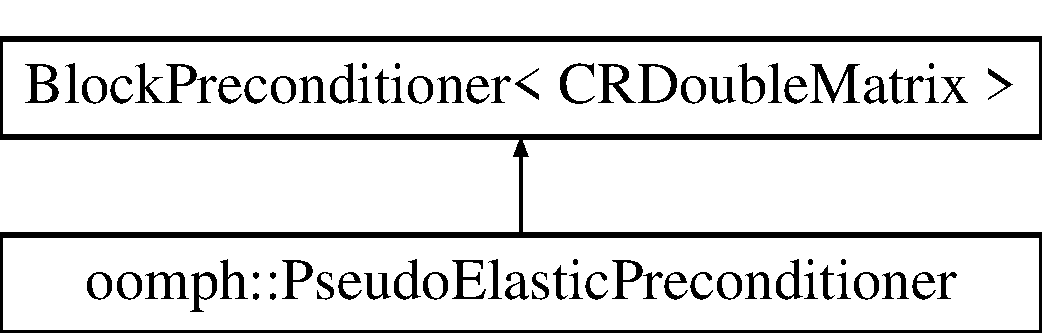
\includegraphics[height=4.000000cm]{classoomph_1_1PseudoElasticPreconditioner}
\end{center}
\end{figure}
\subsection*{Public Types}
\begin{DoxyCompactItemize}
\item 
enum \hyperlink{classoomph_1_1PseudoElasticPreconditioner_acde733e1a111a961d1e714add4e8015d}{Elastic\+\_\+preconditioner\+\_\+type} \{ \hyperlink{classoomph_1_1PseudoElasticPreconditioner_acde733e1a111a961d1e714add4e8015da277774b20738300271de0fa42391a951}{Exact\+\_\+block\+\_\+preconditioner}, 
\hyperlink{classoomph_1_1PseudoElasticPreconditioner_acde733e1a111a961d1e714add4e8015da048620d7667a53bcfb11513dea9b2977}{Block\+\_\+diagonal\+\_\+preconditioner}, 
\hyperlink{classoomph_1_1PseudoElasticPreconditioner_acde733e1a111a961d1e714add4e8015dabf00157409786d29ec7122bb86a5e8fe}{Block\+\_\+lower\+\_\+triangular\+\_\+preconditioner}, 
\hyperlink{classoomph_1_1PseudoElasticPreconditioner_acde733e1a111a961d1e714add4e8015daed4f4716017bc0f8d0c40ed7aaab735e}{Block\+\_\+upper\+\_\+triangular\+\_\+preconditioner}
 \}\begin{DoxyCompactList}\small\item\em The augmented elasticity system can be preconditioned in one of four ways. 0 -\/ Exact preconditioner 1 -\/ Block diagonal preconditioning 2 -\/ Block upper triangular preconditioner 3 -\/ Block lower triangular preconditioner We group together the different components of the displacement vector field for the block decomposition. \end{DoxyCompactList}
\item 
typedef \hyperlink{classoomph_1_1Preconditioner}{Preconditioner} $\ast$($\ast$ \hyperlink{classoomph_1_1PseudoElasticPreconditioner_a1462e1ef48ed2668c06dfd36c783d1a5}{Subsidiary\+Preconditioner\+Fct\+Pt}) ()
\begin{DoxyCompactList}\small\item\em This preconditioner includes the option to use subsidiary operators other than \hyperlink{classoomph_1_1SuperLUPreconditioner}{Super\+L\+U\+Preconditioner} for this problem. This is the typedef of a function that should return an instance of a subsidiary preconditioning operator. This preconditioner is responsible for the destruction of the subsidiary preconditioners. \end{DoxyCompactList}\end{DoxyCompactItemize}
\subsection*{Public Member Functions}
\begin{DoxyCompactItemize}
\item 
\hyperlink{classoomph_1_1PseudoElasticPreconditioner_ab2638e8ccceed850b8eb581fc1309ff0}{Pseudo\+Elastic\+Preconditioner} ()
\begin{DoxyCompactList}\small\item\em Default (and only) constructor. \end{DoxyCompactList}\item 
virtual \hyperlink{classoomph_1_1PseudoElasticPreconditioner_a9366f2553545b09995e40ad8fa4ed91c}{$\sim$\+Pseudo\+Elastic\+Preconditioner} ()
\begin{DoxyCompactList}\small\item\em destructor \end{DoxyCompactList}\item 
\hyperlink{classoomph_1_1PseudoElasticPreconditioner_aaf160121defa770605f1510e222b14bb}{Pseudo\+Elastic\+Preconditioner} (const \hyperlink{classoomph_1_1PseudoElasticPreconditioner}{Pseudo\+Elastic\+Preconditioner} \&)
\begin{DoxyCompactList}\small\item\em Broken copy constructor. \end{DoxyCompactList}\item 
void \hyperlink{classoomph_1_1PseudoElasticPreconditioner_a69909eef3e1530ca7faf48c653ec7327}{setup} ()
\begin{DoxyCompactList}\small\item\em Broken assignment operator. \end{DoxyCompactList}\item 
void \hyperlink{classoomph_1_1PseudoElasticPreconditioner_a2533d2574d2c7d6613fda72b96a5f885}{preconditioner\+\_\+solve} (const \hyperlink{classoomph_1_1DoubleVector}{Double\+Vector} \&r, \hyperlink{classoomph_1_1DoubleVector}{Double\+Vector} \&z)
\begin{DoxyCompactList}\small\item\em Apply the preconditioner. Method implemented in two other methods (elastic and lagrange multiplier subsidiary preocnditioner) for the \hyperlink{classoomph_1_1PseudoElasticFSIPreconditioner}{Pseudo\+Elastic\+F\+S\+I\+Preconditioner}. \end{DoxyCompactList}\item 
void \hyperlink{classoomph_1_1PseudoElasticPreconditioner_ae115b58574a36c2c8fecb2524afa54f1}{set\+\_\+elastic\+\_\+mesh} (\hyperlink{classoomph_1_1Mesh}{Mesh} $\ast$\hyperlink{classoomph_1_1BlockPreconditioner_a3c0e92cb77c3e3179007fe9fd99b6428}{mesh\+\_\+pt})
\begin{DoxyCompactList}\small\item\em Access function to mesh containing the block-\/preconditionable elastic elements. \end{DoxyCompactList}\item 
void \hyperlink{classoomph_1_1PseudoElasticPreconditioner_a6030c2461383ee1a0b8ac6ed56b0daf6}{set\+\_\+lagrange\+\_\+multiplier\+\_\+mesh} (\hyperlink{classoomph_1_1Mesh}{Mesh} $\ast$\hyperlink{classoomph_1_1BlockPreconditioner_a3c0e92cb77c3e3179007fe9fd99b6428}{mesh\+\_\+pt})
\begin{DoxyCompactList}\small\item\em Access function to mesh containing the block-\/preconditionable lagrange multiplier elements. \end{DoxyCompactList}\item 
void \hyperlink{classoomph_1_1PseudoElasticPreconditioner_a917caf20e03fc8bdb45336206ce5365e}{enable\+\_\+inf\+\_\+norm\+\_\+of\+\_\+s\+\_\+scaling} ()
\begin{DoxyCompactList}\small\item\em Call to use the inf norm of S as scaling. \end{DoxyCompactList}\item 
void \hyperlink{classoomph_1_1PseudoElasticPreconditioner_a038e7d2eaea4346c3ea6ba2b34ae824c}{disable\+\_\+inf\+\_\+norm\+\_\+of\+\_\+s\+\_\+scaling} ()
\begin{DoxyCompactList}\small\item\em Call to use no scaling. \end{DoxyCompactList}\item 
void \hyperlink{classoomph_1_1PseudoElasticPreconditioner_a64865a85f35ae9385f9f8d68e75595e0}{set\+\_\+lagrange\+\_\+multiplier\+\_\+subsidiary\+\_\+preconditioner} (\hyperlink{classoomph_1_1PseudoElasticPreconditioner_a1462e1ef48ed2668c06dfd36c783d1a5}{Subsidiary\+Preconditioner\+Fct\+Pt} prec\+\_\+fn)
\begin{DoxyCompactList}\small\item\em By default the Lagrange multiplier subsidiary systems are preconditioner with \hyperlink{classoomph_1_1SuperLUPreconditioner}{Super\+L\+U\+Preconditioner}. For a different preconditioner, pass a function to this method returning a different subsidiary operator. \end{DoxyCompactList}\item 
void \hyperlink{classoomph_1_1PseudoElasticPreconditioner_a8c75fe5786d64a042056df16a062c055}{set\+\_\+elastic\+\_\+subsidiary\+\_\+preconditioner} (\hyperlink{classoomph_1_1PseudoElasticPreconditioner_a1462e1ef48ed2668c06dfd36c783d1a5}{Subsidiary\+Preconditioner\+Fct\+Pt} prec\+\_\+fn)
\begin{DoxyCompactList}\small\item\em By default the elastic subsidiary systems are preconditioner with \hyperlink{classoomph_1_1SuperLUPreconditioner}{Super\+L\+U\+Preconditioner}. For a different preconditioner, pass a function to this method returning a different subsidiary operator. \end{DoxyCompactList}\item 
\hyperlink{classoomph_1_1PseudoElasticPreconditioner_acde733e1a111a961d1e714add4e8015d}{Elastic\+\_\+preconditioner\+\_\+type} \& \hyperlink{classoomph_1_1PseudoElasticPreconditioner_a1bae7b43cffbfbce246b736d9e70f908}{elastic\+\_\+preconditioner\+\_\+type} ()
\begin{DoxyCompactList}\small\item\em Set the type of preconditioner applied to the elastic\+: 0 -\/ Exact preconditioner 1 -\/ Block diagonal preconditioning 2 -\/ Block upper triangular preconditioner 3 -\/ Block lower triangular preconditioner We group together the different components of the displacement vector field for the block decomposition. \end{DoxyCompactList}\item 
void \hyperlink{classoomph_1_1PseudoElasticPreconditioner_adcc9487ec16eea12912b2f3a023b4129}{clean\+\_\+up\+\_\+memory} ()
\begin{DoxyCompactList}\small\item\em Clears the memory. \end{DoxyCompactList}\end{DoxyCompactItemize}
\subsection*{Private Member Functions}
\begin{DoxyCompactItemize}
\item 
void \hyperlink{classoomph_1_1PseudoElasticPreconditioner_a9398dd60b00bc611a5b03e859256b410}{elastic\+\_\+preconditioner\+\_\+solve} (const \hyperlink{classoomph_1_1DoubleVector}{Double\+Vector} \&r, \hyperlink{classoomph_1_1DoubleVector}{Double\+Vector} \&z)
\begin{DoxyCompactList}\small\item\em Apply the elastic subsidiary preconditioner. \end{DoxyCompactList}\item 
void \hyperlink{classoomph_1_1PseudoElasticPreconditioner_a071ddbc46bb55f2c11fe0dfe9b69bb4a}{lagrange\+\_\+multiplier\+\_\+preconditioner\+\_\+solve} (const \hyperlink{classoomph_1_1DoubleVector}{Double\+Vector} \&r, \hyperlink{classoomph_1_1DoubleVector}{Double\+Vector} \&z)
\begin{DoxyCompactList}\small\item\em Apply the lagrange multiplier subsidiary preconditioner. \end{DoxyCompactList}\end{DoxyCompactItemize}
\subsection*{Private Attributes}
\begin{DoxyCompactItemize}
\item 
double \hyperlink{classoomph_1_1PseudoElasticPreconditioner_a3e2302245fa432f49e3f979cbfe6b3a2}{Scaling}
\begin{DoxyCompactList}\small\item\em The scaling. Defaults to infinity norm of S. \end{DoxyCompactList}\item 
bool \hyperlink{classoomph_1_1PseudoElasticPreconditioner_a3ca651eb7983c61cdaea734b19f2ac25}{Use\+\_\+inf\+\_\+norm\+\_\+of\+\_\+s\+\_\+scaling}
\begin{DoxyCompactList}\small\item\em boolean indicating whether the inf-\/norm of S should be used as scaling. Default = true; \end{DoxyCompactList}\item 
\hyperlink{classoomph_1_1PseudoElasticPreconditioner_acde733e1a111a961d1e714add4e8015d}{Elastic\+\_\+preconditioner\+\_\+type} \hyperlink{classoomph_1_1PseudoElasticPreconditioner_abb84100d37f174e683b2d7a0dd688584}{E\+\_\+preconditioner\+\_\+type}
\begin{DoxyCompactList}\small\item\em An unsigned indicating which method should be used for preconditioning the solid component. \end{DoxyCompactList}\item 
unsigned \hyperlink{classoomph_1_1PseudoElasticPreconditioner_aef0a56e6011e3a7f1c3a2ce171949077}{Dim}
\begin{DoxyCompactList}\small\item\em the dimension of the problem \end{DoxyCompactList}\item 
\hyperlink{classoomph_1_1Preconditioner}{Preconditioner} $\ast$ \hyperlink{classoomph_1_1PseudoElasticPreconditioner_ae5cbfeac8ef38461d7816ca01dbd9eb3}{Elastic\+\_\+preconditioner\+\_\+pt}
\begin{DoxyCompactList}\small\item\em storage for the preconditioner for the solid system \end{DoxyCompactList}\item 
\hyperlink{classoomph_1_1Vector}{Vector}$<$ \hyperlink{classoomph_1_1Preconditioner}{Preconditioner} $\ast$ $>$ \hyperlink{classoomph_1_1PseudoElasticPreconditioner_a705470f8265f77b11eb5a5096a9fe59d}{Lagrange\+\_\+multiplier\+\_\+preconditioner\+\_\+pt}
\begin{DoxyCompactList}\small\item\em lagrange multiplier preconditioner pt \end{DoxyCompactList}\item 
\hyperlink{classoomph_1_1PseudoElasticPreconditioner_a1462e1ef48ed2668c06dfd36c783d1a5}{Subsidiary\+Preconditioner\+Fct\+Pt} \hyperlink{classoomph_1_1PseudoElasticPreconditioner_a0206c1e2da88da8948f2d560e8376aa3}{Lagrange\+\_\+multiplier\+\_\+subsidiary\+\_\+preconditioner\+\_\+function\+\_\+pt}
\begin{DoxyCompactList}\small\item\em The Lagrange multiplier subsidiary preconditioner function pointer. \end{DoxyCompactList}\item 
\hyperlink{classoomph_1_1PseudoElasticPreconditioner_a1462e1ef48ed2668c06dfd36c783d1a5}{Subsidiary\+Preconditioner\+Fct\+Pt} \hyperlink{classoomph_1_1PseudoElasticPreconditioner_aa3ca9f5ccba13b8a2038afb386f73b2d}{Elastic\+\_\+subsidiary\+\_\+preconditioner\+\_\+function\+\_\+pt}
\begin{DoxyCompactList}\small\item\em The solid subsidiary preconditioner function pointer. \end{DoxyCompactList}\item 
\hyperlink{classoomph_1_1Mesh}{Mesh} $\ast$ \hyperlink{classoomph_1_1PseudoElasticPreconditioner_aba765545c62b9dc52f7c2ea25ea13177}{Elastic\+\_\+mesh\+\_\+pt}
\begin{DoxyCompactList}\small\item\em Pointer to the mesh containing the solid elements. \end{DoxyCompactList}\item 
\hyperlink{classoomph_1_1Mesh}{Mesh} $\ast$ \hyperlink{classoomph_1_1PseudoElasticPreconditioner_a9d167073db4ade6ba70f036c4ab926dd}{Lagrange\+\_\+multiplier\+\_\+mesh\+\_\+pt}
\begin{DoxyCompactList}\small\item\em Pointer to the mesh containing the Lagrange multiplier elements. \end{DoxyCompactList}\end{DoxyCompactItemize}
\subsection*{Friends}
\begin{DoxyCompactItemize}
\item 
class \hyperlink{classoomph_1_1PseudoElasticPreconditioner_aaaea2b4795566f81945597254305249d}{Pseudo\+Elastic\+F\+S\+I\+Preconditioner}
\begin{DoxyCompactList}\small\item\em \hyperlink{classoomph_1_1PseudoElasticFSIPreconditioner}{Pseudo\+Elastic\+F\+S\+I\+Preconditioner} is a friend to access the private $\ast$\+\_\+preconditioner\+\_\+solve(...) method. \end{DoxyCompactList}\end{DoxyCompactItemize}
\subsection*{Additional Inherited Members}


\subsection{Detailed Description}
A subsidiary preconditioner for the pseudo-\/elastic F\+SI preconditioner. Also a stand-\/alone preconditioner for the problem of non-\/linear elasticity subject to prescribed displacement by Lagrange multiplier. {\bfseries Enumeration} of Elastic D\+OF types in the Pseudo-\/\+Elastic Elements The method get\+\_\+dof\+\_\+types\+\_\+for\+\_\+unknowns() must be implemented such that D\+O\+Fs subject be Lagrange multiplier and D\+O\+Fs N\+OT subject to Lagrange multiplier have different labels. For example in a 3D problem there are 6 D\+OF types and the following labelling must be implemented\+: 0 -\/ x displacement (without lagr mult traction) 1 -\/ y displacement (without lagr mult traction) 2 -\/ z displacement (without lagr mult traction) 4 -\/ x displacement (with lagr mult traction) 5 -\/ y displacement (with lagr mult traction) 6 -\/ z displacement (with lagr mult traction) 

Definition at line 107 of file pseudo\+\_\+elastic\+\_\+preconditioner.\+h.



\subsection{Member Typedef Documentation}
\mbox{\Hypertarget{classoomph_1_1PseudoElasticPreconditioner_a1462e1ef48ed2668c06dfd36c783d1a5}\label{classoomph_1_1PseudoElasticPreconditioner_a1462e1ef48ed2668c06dfd36c783d1a5}} 
\index{oomph\+::\+Pseudo\+Elastic\+Preconditioner@{oomph\+::\+Pseudo\+Elastic\+Preconditioner}!Subsidiary\+Preconditioner\+Fct\+Pt@{Subsidiary\+Preconditioner\+Fct\+Pt}}
\index{Subsidiary\+Preconditioner\+Fct\+Pt@{Subsidiary\+Preconditioner\+Fct\+Pt}!oomph\+::\+Pseudo\+Elastic\+Preconditioner@{oomph\+::\+Pseudo\+Elastic\+Preconditioner}}
\subsubsection{\texorpdfstring{Subsidiary\+Preconditioner\+Fct\+Pt}{SubsidiaryPreconditionerFctPt}}
{\footnotesize\ttfamily typedef \hyperlink{classoomph_1_1Preconditioner}{Preconditioner}$\ast$($\ast$ oomph\+::\+Pseudo\+Elastic\+Preconditioner\+::\+Subsidiary\+Preconditioner\+Fct\+Pt) ()}



This preconditioner includes the option to use subsidiary operators other than \hyperlink{classoomph_1_1SuperLUPreconditioner}{Super\+L\+U\+Preconditioner} for this problem. This is the typedef of a function that should return an instance of a subsidiary preconditioning operator. This preconditioner is responsible for the destruction of the subsidiary preconditioners. 



Definition at line 121 of file pseudo\+\_\+elastic\+\_\+preconditioner.\+h.



\subsection{Member Enumeration Documentation}
\mbox{\Hypertarget{classoomph_1_1PseudoElasticPreconditioner_acde733e1a111a961d1e714add4e8015d}\label{classoomph_1_1PseudoElasticPreconditioner_acde733e1a111a961d1e714add4e8015d}} 
\index{oomph\+::\+Pseudo\+Elastic\+Preconditioner@{oomph\+::\+Pseudo\+Elastic\+Preconditioner}!Elastic\+\_\+preconditioner\+\_\+type@{Elastic\+\_\+preconditioner\+\_\+type}}
\index{Elastic\+\_\+preconditioner\+\_\+type@{Elastic\+\_\+preconditioner\+\_\+type}!oomph\+::\+Pseudo\+Elastic\+Preconditioner@{oomph\+::\+Pseudo\+Elastic\+Preconditioner}}
\subsubsection{\texorpdfstring{Elastic\+\_\+preconditioner\+\_\+type}{Elastic\_preconditioner\_type}}
{\footnotesize\ttfamily enum \hyperlink{classoomph_1_1PseudoElasticPreconditioner_acde733e1a111a961d1e714add4e8015d}{oomph\+::\+Pseudo\+Elastic\+Preconditioner\+::\+Elastic\+\_\+preconditioner\+\_\+type}}



The augmented elasticity system can be preconditioned in one of four ways. 0 -\/ Exact preconditioner 1 -\/ Block diagonal preconditioning 2 -\/ Block upper triangular preconditioner 3 -\/ Block lower triangular preconditioner We group together the different components of the displacement vector field for the block decomposition. 

\begin{DoxyEnumFields}{Enumerator}
\raisebox{\heightof{T}}[0pt][0pt]{\index{Exact\+\_\+block\+\_\+preconditioner@{Exact\+\_\+block\+\_\+preconditioner}!oomph\+::\+Pseudo\+Elastic\+Preconditioner@{oomph\+::\+Pseudo\+Elastic\+Preconditioner}}\index{oomph\+::\+Pseudo\+Elastic\+Preconditioner@{oomph\+::\+Pseudo\+Elastic\+Preconditioner}!Exact\+\_\+block\+\_\+preconditioner@{Exact\+\_\+block\+\_\+preconditioner}}}\mbox{\Hypertarget{classoomph_1_1PseudoElasticPreconditioner_acde733e1a111a961d1e714add4e8015da277774b20738300271de0fa42391a951}\label{classoomph_1_1PseudoElasticPreconditioner_acde733e1a111a961d1e714add4e8015da277774b20738300271de0fa42391a951}} 
Exact\+\_\+block\+\_\+preconditioner&\\
\hline

\raisebox{\heightof{T}}[0pt][0pt]{\index{Block\+\_\+diagonal\+\_\+preconditioner@{Block\+\_\+diagonal\+\_\+preconditioner}!oomph\+::\+Pseudo\+Elastic\+Preconditioner@{oomph\+::\+Pseudo\+Elastic\+Preconditioner}}\index{oomph\+::\+Pseudo\+Elastic\+Preconditioner@{oomph\+::\+Pseudo\+Elastic\+Preconditioner}!Block\+\_\+diagonal\+\_\+preconditioner@{Block\+\_\+diagonal\+\_\+preconditioner}}}\mbox{\Hypertarget{classoomph_1_1PseudoElasticPreconditioner_acde733e1a111a961d1e714add4e8015da048620d7667a53bcfb11513dea9b2977}\label{classoomph_1_1PseudoElasticPreconditioner_acde733e1a111a961d1e714add4e8015da048620d7667a53bcfb11513dea9b2977}} 
Block\+\_\+diagonal\+\_\+preconditioner&\\
\hline

\raisebox{\heightof{T}}[0pt][0pt]{\index{Block\+\_\+lower\+\_\+triangular\+\_\+preconditioner@{Block\+\_\+lower\+\_\+triangular\+\_\+preconditioner}!oomph\+::\+Pseudo\+Elastic\+Preconditioner@{oomph\+::\+Pseudo\+Elastic\+Preconditioner}}\index{oomph\+::\+Pseudo\+Elastic\+Preconditioner@{oomph\+::\+Pseudo\+Elastic\+Preconditioner}!Block\+\_\+lower\+\_\+triangular\+\_\+preconditioner@{Block\+\_\+lower\+\_\+triangular\+\_\+preconditioner}}}\mbox{\Hypertarget{classoomph_1_1PseudoElasticPreconditioner_acde733e1a111a961d1e714add4e8015dabf00157409786d29ec7122bb86a5e8fe}\label{classoomph_1_1PseudoElasticPreconditioner_acde733e1a111a961d1e714add4e8015dabf00157409786d29ec7122bb86a5e8fe}} 
Block\+\_\+lower\+\_\+triangular\+\_\+preconditioner&\\
\hline

\raisebox{\heightof{T}}[0pt][0pt]{\index{Block\+\_\+upper\+\_\+triangular\+\_\+preconditioner@{Block\+\_\+upper\+\_\+triangular\+\_\+preconditioner}!oomph\+::\+Pseudo\+Elastic\+Preconditioner@{oomph\+::\+Pseudo\+Elastic\+Preconditioner}}\index{oomph\+::\+Pseudo\+Elastic\+Preconditioner@{oomph\+::\+Pseudo\+Elastic\+Preconditioner}!Block\+\_\+upper\+\_\+triangular\+\_\+preconditioner@{Block\+\_\+upper\+\_\+triangular\+\_\+preconditioner}}}\mbox{\Hypertarget{classoomph_1_1PseudoElasticPreconditioner_acde733e1a111a961d1e714add4e8015daed4f4716017bc0f8d0c40ed7aaab735e}\label{classoomph_1_1PseudoElasticPreconditioner_acde733e1a111a961d1e714add4e8015daed4f4716017bc0f8d0c40ed7aaab735e}} 
Block\+\_\+upper\+\_\+triangular\+\_\+preconditioner&\\
\hline

\end{DoxyEnumFields}


Definition at line 131 of file pseudo\+\_\+elastic\+\_\+preconditioner.\+h.



\subsection{Constructor \& Destructor Documentation}
\mbox{\Hypertarget{classoomph_1_1PseudoElasticPreconditioner_ab2638e8ccceed850b8eb581fc1309ff0}\label{classoomph_1_1PseudoElasticPreconditioner_ab2638e8ccceed850b8eb581fc1309ff0}} 
\index{oomph\+::\+Pseudo\+Elastic\+Preconditioner@{oomph\+::\+Pseudo\+Elastic\+Preconditioner}!Pseudo\+Elastic\+Preconditioner@{Pseudo\+Elastic\+Preconditioner}}
\index{Pseudo\+Elastic\+Preconditioner@{Pseudo\+Elastic\+Preconditioner}!oomph\+::\+Pseudo\+Elastic\+Preconditioner@{oomph\+::\+Pseudo\+Elastic\+Preconditioner}}
\subsubsection{\texorpdfstring{Pseudo\+Elastic\+Preconditioner()}{PseudoElasticPreconditioner()}\hspace{0.1cm}{\footnotesize\ttfamily [1/2]}}
{\footnotesize\ttfamily oomph\+::\+Pseudo\+Elastic\+Preconditioner\+::\+Pseudo\+Elastic\+Preconditioner (\begin{DoxyParamCaption}{ }\end{DoxyParamCaption})\hspace{0.3cm}{\ttfamily [inline]}}



Default (and only) constructor. 



Definition at line 137 of file pseudo\+\_\+elastic\+\_\+preconditioner.\+h.

\mbox{\Hypertarget{classoomph_1_1PseudoElasticPreconditioner_a9366f2553545b09995e40ad8fa4ed91c}\label{classoomph_1_1PseudoElasticPreconditioner_a9366f2553545b09995e40ad8fa4ed91c}} 
\index{oomph\+::\+Pseudo\+Elastic\+Preconditioner@{oomph\+::\+Pseudo\+Elastic\+Preconditioner}!````~Pseudo\+Elastic\+Preconditioner@{$\sim$\+Pseudo\+Elastic\+Preconditioner}}
\index{````~Pseudo\+Elastic\+Preconditioner@{$\sim$\+Pseudo\+Elastic\+Preconditioner}!oomph\+::\+Pseudo\+Elastic\+Preconditioner@{oomph\+::\+Pseudo\+Elastic\+Preconditioner}}
\subsubsection{\texorpdfstring{$\sim$\+Pseudo\+Elastic\+Preconditioner()}{~PseudoElasticPreconditioner()}}
{\footnotesize\ttfamily virtual oomph\+::\+Pseudo\+Elastic\+Preconditioner\+::$\sim$\+Pseudo\+Elastic\+Preconditioner (\begin{DoxyParamCaption}{ }\end{DoxyParamCaption})\hspace{0.3cm}{\ttfamily [inline]}, {\ttfamily [virtual]}}



destructor 



Definition at line 154 of file pseudo\+\_\+elastic\+\_\+preconditioner.\+h.

\mbox{\Hypertarget{classoomph_1_1PseudoElasticPreconditioner_aaf160121defa770605f1510e222b14bb}\label{classoomph_1_1PseudoElasticPreconditioner_aaf160121defa770605f1510e222b14bb}} 
\index{oomph\+::\+Pseudo\+Elastic\+Preconditioner@{oomph\+::\+Pseudo\+Elastic\+Preconditioner}!Pseudo\+Elastic\+Preconditioner@{Pseudo\+Elastic\+Preconditioner}}
\index{Pseudo\+Elastic\+Preconditioner@{Pseudo\+Elastic\+Preconditioner}!oomph\+::\+Pseudo\+Elastic\+Preconditioner@{oomph\+::\+Pseudo\+Elastic\+Preconditioner}}
\subsubsection{\texorpdfstring{Pseudo\+Elastic\+Preconditioner()}{PseudoElasticPreconditioner()}\hspace{0.1cm}{\footnotesize\ttfamily [2/2]}}
{\footnotesize\ttfamily oomph\+::\+Pseudo\+Elastic\+Preconditioner\+::\+Pseudo\+Elastic\+Preconditioner (\begin{DoxyParamCaption}\item[{const \hyperlink{classoomph_1_1PseudoElasticPreconditioner}{Pseudo\+Elastic\+Preconditioner} \&}]{ }\end{DoxyParamCaption})\hspace{0.3cm}{\ttfamily [inline]}}



Broken copy constructor. 



Definition at line 161 of file pseudo\+\_\+elastic\+\_\+preconditioner.\+h.



References oomph\+::\+Broken\+Copy\+::broken\+\_\+copy(), and oomph\+::\+Terminate\+Helper\+::setup().



\subsection{Member Function Documentation}
\mbox{\Hypertarget{classoomph_1_1PseudoElasticPreconditioner_adcc9487ec16eea12912b2f3a023b4129}\label{classoomph_1_1PseudoElasticPreconditioner_adcc9487ec16eea12912b2f3a023b4129}} 
\index{oomph\+::\+Pseudo\+Elastic\+Preconditioner@{oomph\+::\+Pseudo\+Elastic\+Preconditioner}!clean\+\_\+up\+\_\+memory@{clean\+\_\+up\+\_\+memory}}
\index{clean\+\_\+up\+\_\+memory@{clean\+\_\+up\+\_\+memory}!oomph\+::\+Pseudo\+Elastic\+Preconditioner@{oomph\+::\+Pseudo\+Elastic\+Preconditioner}}
\subsubsection{\texorpdfstring{clean\+\_\+up\+\_\+memory()}{clean\_up\_memory()}}
{\footnotesize\ttfamily void oomph\+::\+Pseudo\+Elastic\+Preconditioner\+::clean\+\_\+up\+\_\+memory (\begin{DoxyParamCaption}{ }\end{DoxyParamCaption})\hspace{0.3cm}{\ttfamily [virtual]}}



Clears the memory. 



Reimplemented from \hyperlink{classoomph_1_1Preconditioner_a46c31c416829bedcd9db238431262027}{oomph\+::\+Preconditioner}.



Definition at line 537 of file pseudo\+\_\+elastic\+\_\+preconditioner.\+cc.



References i.



Referenced by oomph\+::\+Pseudo\+Elastic\+F\+S\+I\+Preconditioner\+::clean\+\_\+up\+\_\+memory().

\mbox{\Hypertarget{classoomph_1_1PseudoElasticPreconditioner_a038e7d2eaea4346c3ea6ba2b34ae824c}\label{classoomph_1_1PseudoElasticPreconditioner_a038e7d2eaea4346c3ea6ba2b34ae824c}} 
\index{oomph\+::\+Pseudo\+Elastic\+Preconditioner@{oomph\+::\+Pseudo\+Elastic\+Preconditioner}!disable\+\_\+inf\+\_\+norm\+\_\+of\+\_\+s\+\_\+scaling@{disable\+\_\+inf\+\_\+norm\+\_\+of\+\_\+s\+\_\+scaling}}
\index{disable\+\_\+inf\+\_\+norm\+\_\+of\+\_\+s\+\_\+scaling@{disable\+\_\+inf\+\_\+norm\+\_\+of\+\_\+s\+\_\+scaling}!oomph\+::\+Pseudo\+Elastic\+Preconditioner@{oomph\+::\+Pseudo\+Elastic\+Preconditioner}}
\subsubsection{\texorpdfstring{disable\+\_\+inf\+\_\+norm\+\_\+of\+\_\+s\+\_\+scaling()}{disable\_inf\_norm\_of\_s\_scaling()}}
{\footnotesize\ttfamily void oomph\+::\+Pseudo\+Elastic\+Preconditioner\+::disable\+\_\+inf\+\_\+norm\+\_\+of\+\_\+s\+\_\+scaling (\begin{DoxyParamCaption}{ }\end{DoxyParamCaption})\hspace{0.3cm}{\ttfamily [inline]}}



Call to use no scaling. 



Definition at line 208 of file pseudo\+\_\+elastic\+\_\+preconditioner.\+h.

\mbox{\Hypertarget{classoomph_1_1PseudoElasticPreconditioner_a9398dd60b00bc611a5b03e859256b410}\label{classoomph_1_1PseudoElasticPreconditioner_a9398dd60b00bc611a5b03e859256b410}} 
\index{oomph\+::\+Pseudo\+Elastic\+Preconditioner@{oomph\+::\+Pseudo\+Elastic\+Preconditioner}!elastic\+\_\+preconditioner\+\_\+solve@{elastic\+\_\+preconditioner\+\_\+solve}}
\index{elastic\+\_\+preconditioner\+\_\+solve@{elastic\+\_\+preconditioner\+\_\+solve}!oomph\+::\+Pseudo\+Elastic\+Preconditioner@{oomph\+::\+Pseudo\+Elastic\+Preconditioner}}
\subsubsection{\texorpdfstring{elastic\+\_\+preconditioner\+\_\+solve()}{elastic\_preconditioner\_solve()}}
{\footnotesize\ttfamily void oomph\+::\+Pseudo\+Elastic\+Preconditioner\+::elastic\+\_\+preconditioner\+\_\+solve (\begin{DoxyParamCaption}\item[{const \hyperlink{classoomph_1_1DoubleVector}{Double\+Vector} \&}]{r,  }\item[{\hyperlink{classoomph_1_1DoubleVector}{Double\+Vector} \&}]{z }\end{DoxyParamCaption})\hspace{0.3cm}{\ttfamily [private]}}



Apply the elastic subsidiary preconditioner. 



Definition at line 503 of file pseudo\+\_\+elastic\+\_\+preconditioner.\+cc.



References lagrange\+\_\+multiplier\+\_\+preconditioner\+\_\+solve().



Referenced by oomph\+::\+Pseudo\+Elastic\+F\+S\+I\+Preconditioner\+::preconditioner\+\_\+solve(), and setup().

\mbox{\Hypertarget{classoomph_1_1PseudoElasticPreconditioner_a1bae7b43cffbfbce246b736d9e70f908}\label{classoomph_1_1PseudoElasticPreconditioner_a1bae7b43cffbfbce246b736d9e70f908}} 
\index{oomph\+::\+Pseudo\+Elastic\+Preconditioner@{oomph\+::\+Pseudo\+Elastic\+Preconditioner}!elastic\+\_\+preconditioner\+\_\+type@{elastic\+\_\+preconditioner\+\_\+type}}
\index{elastic\+\_\+preconditioner\+\_\+type@{elastic\+\_\+preconditioner\+\_\+type}!oomph\+::\+Pseudo\+Elastic\+Preconditioner@{oomph\+::\+Pseudo\+Elastic\+Preconditioner}}
\subsubsection{\texorpdfstring{elastic\+\_\+preconditioner\+\_\+type()}{elastic\_preconditioner\_type()}}
{\footnotesize\ttfamily \hyperlink{classoomph_1_1PseudoElasticPreconditioner_acde733e1a111a961d1e714add4e8015d}{Elastic\+\_\+preconditioner\+\_\+type}\& oomph\+::\+Pseudo\+Elastic\+Preconditioner\+::elastic\+\_\+preconditioner\+\_\+type (\begin{DoxyParamCaption}{ }\end{DoxyParamCaption})\hspace{0.3cm}{\ttfamily [inline]}}



Set the type of preconditioner applied to the elastic\+: 0 -\/ Exact preconditioner 1 -\/ Block diagonal preconditioning 2 -\/ Block upper triangular preconditioner 3 -\/ Block lower triangular preconditioner We group together the different components of the displacement vector field for the block decomposition. 



Definition at line 238 of file pseudo\+\_\+elastic\+\_\+preconditioner.\+h.

\mbox{\Hypertarget{classoomph_1_1PseudoElasticPreconditioner_a917caf20e03fc8bdb45336206ce5365e}\label{classoomph_1_1PseudoElasticPreconditioner_a917caf20e03fc8bdb45336206ce5365e}} 
\index{oomph\+::\+Pseudo\+Elastic\+Preconditioner@{oomph\+::\+Pseudo\+Elastic\+Preconditioner}!enable\+\_\+inf\+\_\+norm\+\_\+of\+\_\+s\+\_\+scaling@{enable\+\_\+inf\+\_\+norm\+\_\+of\+\_\+s\+\_\+scaling}}
\index{enable\+\_\+inf\+\_\+norm\+\_\+of\+\_\+s\+\_\+scaling@{enable\+\_\+inf\+\_\+norm\+\_\+of\+\_\+s\+\_\+scaling}!oomph\+::\+Pseudo\+Elastic\+Preconditioner@{oomph\+::\+Pseudo\+Elastic\+Preconditioner}}
\subsubsection{\texorpdfstring{enable\+\_\+inf\+\_\+norm\+\_\+of\+\_\+s\+\_\+scaling()}{enable\_inf\_norm\_of\_s\_scaling()}}
{\footnotesize\ttfamily void oomph\+::\+Pseudo\+Elastic\+Preconditioner\+::enable\+\_\+inf\+\_\+norm\+\_\+of\+\_\+s\+\_\+scaling (\begin{DoxyParamCaption}{ }\end{DoxyParamCaption})\hspace{0.3cm}{\ttfamily [inline]}}



Call to use the inf norm of S as scaling. 



Definition at line 204 of file pseudo\+\_\+elastic\+\_\+preconditioner.\+h.

\mbox{\Hypertarget{classoomph_1_1PseudoElasticPreconditioner_a071ddbc46bb55f2c11fe0dfe9b69bb4a}\label{classoomph_1_1PseudoElasticPreconditioner_a071ddbc46bb55f2c11fe0dfe9b69bb4a}} 
\index{oomph\+::\+Pseudo\+Elastic\+Preconditioner@{oomph\+::\+Pseudo\+Elastic\+Preconditioner}!lagrange\+\_\+multiplier\+\_\+preconditioner\+\_\+solve@{lagrange\+\_\+multiplier\+\_\+preconditioner\+\_\+solve}}
\index{lagrange\+\_\+multiplier\+\_\+preconditioner\+\_\+solve@{lagrange\+\_\+multiplier\+\_\+preconditioner\+\_\+solve}!oomph\+::\+Pseudo\+Elastic\+Preconditioner@{oomph\+::\+Pseudo\+Elastic\+Preconditioner}}
\subsubsection{\texorpdfstring{lagrange\+\_\+multiplier\+\_\+preconditioner\+\_\+solve()}{lagrange\_multiplier\_preconditioner\_solve()}}
{\footnotesize\ttfamily void oomph\+::\+Pseudo\+Elastic\+Preconditioner\+::lagrange\+\_\+multiplier\+\_\+preconditioner\+\_\+solve (\begin{DoxyParamCaption}\item[{const \hyperlink{classoomph_1_1DoubleVector}{Double\+Vector} \&}]{r,  }\item[{\hyperlink{classoomph_1_1DoubleVector}{Double\+Vector} \&}]{z }\end{DoxyParamCaption})\hspace{0.3cm}{\ttfamily [private]}}



Apply the lagrange multiplier subsidiary preconditioner. 



Definition at line 513 of file pseudo\+\_\+elastic\+\_\+preconditioner.\+cc.



References oomph\+::\+Multi\+\_\+domain\+\_\+functions\+::\+Dim, i, oomph\+::\+Distributable\+Linear\+Algebra\+Object\+::nrow\+\_\+local(), and oomph\+::\+Double\+Vector\+::values\+\_\+pt().



Referenced by elastic\+\_\+preconditioner\+\_\+solve().

\mbox{\Hypertarget{classoomph_1_1PseudoElasticPreconditioner_a2533d2574d2c7d6613fda72b96a5f885}\label{classoomph_1_1PseudoElasticPreconditioner_a2533d2574d2c7d6613fda72b96a5f885}} 
\index{oomph\+::\+Pseudo\+Elastic\+Preconditioner@{oomph\+::\+Pseudo\+Elastic\+Preconditioner}!preconditioner\+\_\+solve@{preconditioner\+\_\+solve}}
\index{preconditioner\+\_\+solve@{preconditioner\+\_\+solve}!oomph\+::\+Pseudo\+Elastic\+Preconditioner@{oomph\+::\+Pseudo\+Elastic\+Preconditioner}}
\subsubsection{\texorpdfstring{preconditioner\+\_\+solve()}{preconditioner\_solve()}}
{\footnotesize\ttfamily void oomph\+::\+Pseudo\+Elastic\+Preconditioner\+::preconditioner\+\_\+solve (\begin{DoxyParamCaption}\item[{const \hyperlink{classoomph_1_1DoubleVector}{Double\+Vector} \&}]{r,  }\item[{\hyperlink{classoomph_1_1DoubleVector}{Double\+Vector} \&}]{z }\end{DoxyParamCaption})\hspace{0.3cm}{\ttfamily [inline]}, {\ttfamily [virtual]}}



Apply the preconditioner. Method implemented in two other methods (elastic and lagrange multiplier subsidiary preocnditioner) for the \hyperlink{classoomph_1_1PseudoElasticFSIPreconditioner}{Pseudo\+Elastic\+F\+S\+I\+Preconditioner}. 



Implements \hyperlink{classoomph_1_1Preconditioner_ace1199369e4465cd2b9a34884bb64ec8}{oomph\+::\+Preconditioner}.



Definition at line 183 of file pseudo\+\_\+elastic\+\_\+preconditioner.\+h.

\mbox{\Hypertarget{classoomph_1_1PseudoElasticPreconditioner_ae115b58574a36c2c8fecb2524afa54f1}\label{classoomph_1_1PseudoElasticPreconditioner_ae115b58574a36c2c8fecb2524afa54f1}} 
\index{oomph\+::\+Pseudo\+Elastic\+Preconditioner@{oomph\+::\+Pseudo\+Elastic\+Preconditioner}!set\+\_\+elastic\+\_\+mesh@{set\+\_\+elastic\+\_\+mesh}}
\index{set\+\_\+elastic\+\_\+mesh@{set\+\_\+elastic\+\_\+mesh}!oomph\+::\+Pseudo\+Elastic\+Preconditioner@{oomph\+::\+Pseudo\+Elastic\+Preconditioner}}
\subsubsection{\texorpdfstring{set\+\_\+elastic\+\_\+mesh()}{set\_elastic\_mesh()}}
{\footnotesize\ttfamily void oomph\+::\+Pseudo\+Elastic\+Preconditioner\+::set\+\_\+elastic\+\_\+mesh (\begin{DoxyParamCaption}\item[{\hyperlink{classoomph_1_1Mesh}{Mesh} $\ast$}]{mesh\+\_\+pt }\end{DoxyParamCaption})\hspace{0.3cm}{\ttfamily [inline]}}



Access function to mesh containing the block-\/preconditionable elastic elements. 



Definition at line 191 of file pseudo\+\_\+elastic\+\_\+preconditioner.\+h.

\mbox{\Hypertarget{classoomph_1_1PseudoElasticPreconditioner_a8c75fe5786d64a042056df16a062c055}\label{classoomph_1_1PseudoElasticPreconditioner_a8c75fe5786d64a042056df16a062c055}} 
\index{oomph\+::\+Pseudo\+Elastic\+Preconditioner@{oomph\+::\+Pseudo\+Elastic\+Preconditioner}!set\+\_\+elastic\+\_\+subsidiary\+\_\+preconditioner@{set\+\_\+elastic\+\_\+subsidiary\+\_\+preconditioner}}
\index{set\+\_\+elastic\+\_\+subsidiary\+\_\+preconditioner@{set\+\_\+elastic\+\_\+subsidiary\+\_\+preconditioner}!oomph\+::\+Pseudo\+Elastic\+Preconditioner@{oomph\+::\+Pseudo\+Elastic\+Preconditioner}}
\subsubsection{\texorpdfstring{set\+\_\+elastic\+\_\+subsidiary\+\_\+preconditioner()}{set\_elastic\_subsidiary\_preconditioner()}}
{\footnotesize\ttfamily void oomph\+::\+Pseudo\+Elastic\+Preconditioner\+::set\+\_\+elastic\+\_\+subsidiary\+\_\+preconditioner (\begin{DoxyParamCaption}\item[{\hyperlink{classoomph_1_1PseudoElasticPreconditioner_a1462e1ef48ed2668c06dfd36c783d1a5}{Subsidiary\+Preconditioner\+Fct\+Pt}}]{prec\+\_\+fn }\end{DoxyParamCaption})\hspace{0.3cm}{\ttfamily [inline]}}



By default the elastic subsidiary systems are preconditioner with \hyperlink{classoomph_1_1SuperLUPreconditioner}{Super\+L\+U\+Preconditioner}. For a different preconditioner, pass a function to this method returning a different subsidiary operator. 



Definition at line 226 of file pseudo\+\_\+elastic\+\_\+preconditioner.\+h.

\mbox{\Hypertarget{classoomph_1_1PseudoElasticPreconditioner_a6030c2461383ee1a0b8ac6ed56b0daf6}\label{classoomph_1_1PseudoElasticPreconditioner_a6030c2461383ee1a0b8ac6ed56b0daf6}} 
\index{oomph\+::\+Pseudo\+Elastic\+Preconditioner@{oomph\+::\+Pseudo\+Elastic\+Preconditioner}!set\+\_\+lagrange\+\_\+multiplier\+\_\+mesh@{set\+\_\+lagrange\+\_\+multiplier\+\_\+mesh}}
\index{set\+\_\+lagrange\+\_\+multiplier\+\_\+mesh@{set\+\_\+lagrange\+\_\+multiplier\+\_\+mesh}!oomph\+::\+Pseudo\+Elastic\+Preconditioner@{oomph\+::\+Pseudo\+Elastic\+Preconditioner}}
\subsubsection{\texorpdfstring{set\+\_\+lagrange\+\_\+multiplier\+\_\+mesh()}{set\_lagrange\_multiplier\_mesh()}}
{\footnotesize\ttfamily void oomph\+::\+Pseudo\+Elastic\+Preconditioner\+::set\+\_\+lagrange\+\_\+multiplier\+\_\+mesh (\begin{DoxyParamCaption}\item[{\hyperlink{classoomph_1_1Mesh}{Mesh} $\ast$}]{mesh\+\_\+pt }\end{DoxyParamCaption})\hspace{0.3cm}{\ttfamily [inline]}}



Access function to mesh containing the block-\/preconditionable lagrange multiplier elements. 



Definition at line 198 of file pseudo\+\_\+elastic\+\_\+preconditioner.\+h.

\mbox{\Hypertarget{classoomph_1_1PseudoElasticPreconditioner_a64865a85f35ae9385f9f8d68e75595e0}\label{classoomph_1_1PseudoElasticPreconditioner_a64865a85f35ae9385f9f8d68e75595e0}} 
\index{oomph\+::\+Pseudo\+Elastic\+Preconditioner@{oomph\+::\+Pseudo\+Elastic\+Preconditioner}!set\+\_\+lagrange\+\_\+multiplier\+\_\+subsidiary\+\_\+preconditioner@{set\+\_\+lagrange\+\_\+multiplier\+\_\+subsidiary\+\_\+preconditioner}}
\index{set\+\_\+lagrange\+\_\+multiplier\+\_\+subsidiary\+\_\+preconditioner@{set\+\_\+lagrange\+\_\+multiplier\+\_\+subsidiary\+\_\+preconditioner}!oomph\+::\+Pseudo\+Elastic\+Preconditioner@{oomph\+::\+Pseudo\+Elastic\+Preconditioner}}
\subsubsection{\texorpdfstring{set\+\_\+lagrange\+\_\+multiplier\+\_\+subsidiary\+\_\+preconditioner()}{set\_lagrange\_multiplier\_subsidiary\_preconditioner()}}
{\footnotesize\ttfamily void oomph\+::\+Pseudo\+Elastic\+Preconditioner\+::set\+\_\+lagrange\+\_\+multiplier\+\_\+subsidiary\+\_\+preconditioner (\begin{DoxyParamCaption}\item[{\hyperlink{classoomph_1_1PseudoElasticPreconditioner_a1462e1ef48ed2668c06dfd36c783d1a5}{Subsidiary\+Preconditioner\+Fct\+Pt}}]{prec\+\_\+fn }\end{DoxyParamCaption})\hspace{0.3cm}{\ttfamily [inline]}}



By default the Lagrange multiplier subsidiary systems are preconditioner with \hyperlink{classoomph_1_1SuperLUPreconditioner}{Super\+L\+U\+Preconditioner}. For a different preconditioner, pass a function to this method returning a different subsidiary operator. 



Definition at line 216 of file pseudo\+\_\+elastic\+\_\+preconditioner.\+h.

\mbox{\Hypertarget{classoomph_1_1PseudoElasticPreconditioner_a69909eef3e1530ca7faf48c653ec7327}\label{classoomph_1_1PseudoElasticPreconditioner_a69909eef3e1530ca7faf48c653ec7327}} 
\index{oomph\+::\+Pseudo\+Elastic\+Preconditioner@{oomph\+::\+Pseudo\+Elastic\+Preconditioner}!setup@{setup}}
\index{setup@{setup}!oomph\+::\+Pseudo\+Elastic\+Preconditioner@{oomph\+::\+Pseudo\+Elastic\+Preconditioner}}
\subsubsection{\texorpdfstring{setup()}{setup()}}
{\footnotesize\ttfamily void oomph\+::\+Pseudo\+Elastic\+Preconditioner\+::setup (\begin{DoxyParamCaption}{ }\end{DoxyParamCaption})\hspace{0.3cm}{\ttfamily [virtual]}}



Broken assignment operator. 

Setup method for the \hyperlink{classoomph_1_1PseudoElasticPreconditioner}{Pseudo\+Elastic\+Preconditioner}. 

Implements \hyperlink{classoomph_1_1Preconditioner_af4886f4efe510e5c9b0eb19422943588}{oomph\+::\+Preconditioner}.



Definition at line 121 of file pseudo\+\_\+elastic\+\_\+preconditioner.\+cc.



References oomph\+::\+Multi\+\_\+domain\+\_\+functions\+::\+Dim, elastic\+\_\+preconditioner\+\_\+solve(), i, oomph\+::\+C\+R\+Double\+Matrix\+Helpers\+::inf\+\_\+norm(), oomph\+::\+Block\+Triangular\+Preconditioner$<$ M\+A\+T\+R\+I\+X $>$\+::lower\+\_\+triangular(), oomph\+::\+Dense\+Matrix$<$ T $>$\+::resize(), oomph\+::\+General\+Purpose\+Block\+Preconditioner$<$ M\+A\+T\+R\+I\+X $>$\+::set\+\_\+dof\+\_\+to\+\_\+block\+\_\+map(), oomph\+::\+General\+Purpose\+Block\+Preconditioner$<$ M\+A\+T\+R\+I\+X $>$\+::set\+\_\+subsidiary\+\_\+preconditioner\+\_\+function(), oomph\+::\+Super\+L\+U\+Preconditioner\+::setup(), oomph\+::\+Block\+Preconditioner$<$ M\+A\+T\+R\+I\+X $>$\+::turn\+\_\+into\+\_\+subsidiary\+\_\+block\+\_\+preconditioner(), and oomph\+::\+Block\+Triangular\+Preconditioner$<$ M\+A\+T\+R\+I\+X $>$\+::upper\+\_\+triangular().



\subsection{Friends And Related Function Documentation}
\mbox{\Hypertarget{classoomph_1_1PseudoElasticPreconditioner_aaaea2b4795566f81945597254305249d}\label{classoomph_1_1PseudoElasticPreconditioner_aaaea2b4795566f81945597254305249d}} 
\index{oomph\+::\+Pseudo\+Elastic\+Preconditioner@{oomph\+::\+Pseudo\+Elastic\+Preconditioner}!Pseudo\+Elastic\+F\+S\+I\+Preconditioner@{Pseudo\+Elastic\+F\+S\+I\+Preconditioner}}
\index{Pseudo\+Elastic\+F\+S\+I\+Preconditioner@{Pseudo\+Elastic\+F\+S\+I\+Preconditioner}!oomph\+::\+Pseudo\+Elastic\+Preconditioner@{oomph\+::\+Pseudo\+Elastic\+Preconditioner}}
\subsubsection{\texorpdfstring{Pseudo\+Elastic\+F\+S\+I\+Preconditioner}{PseudoElasticFSIPreconditioner}}
{\footnotesize\ttfamily friend class \hyperlink{classoomph_1_1PseudoElasticFSIPreconditioner}{Pseudo\+Elastic\+F\+S\+I\+Preconditioner}\hspace{0.3cm}{\ttfamily [friend]}}



\hyperlink{classoomph_1_1PseudoElasticFSIPreconditioner}{Pseudo\+Elastic\+F\+S\+I\+Preconditioner} is a friend to access the private $\ast$\+\_\+preconditioner\+\_\+solve(...) method. 



Definition at line 112 of file pseudo\+\_\+elastic\+\_\+preconditioner.\+h.



\subsection{Member Data Documentation}
\mbox{\Hypertarget{classoomph_1_1PseudoElasticPreconditioner_aef0a56e6011e3a7f1c3a2ce171949077}\label{classoomph_1_1PseudoElasticPreconditioner_aef0a56e6011e3a7f1c3a2ce171949077}} 
\index{oomph\+::\+Pseudo\+Elastic\+Preconditioner@{oomph\+::\+Pseudo\+Elastic\+Preconditioner}!Dim@{Dim}}
\index{Dim@{Dim}!oomph\+::\+Pseudo\+Elastic\+Preconditioner@{oomph\+::\+Pseudo\+Elastic\+Preconditioner}}
\subsubsection{\texorpdfstring{Dim}{Dim}}
{\footnotesize\ttfamily unsigned oomph\+::\+Pseudo\+Elastic\+Preconditioner\+::\+Dim\hspace{0.3cm}{\ttfamily [private]}}



the dimension of the problem 



Definition at line 267 of file pseudo\+\_\+elastic\+\_\+preconditioner.\+h.

\mbox{\Hypertarget{classoomph_1_1PseudoElasticPreconditioner_abb84100d37f174e683b2d7a0dd688584}\label{classoomph_1_1PseudoElasticPreconditioner_abb84100d37f174e683b2d7a0dd688584}} 
\index{oomph\+::\+Pseudo\+Elastic\+Preconditioner@{oomph\+::\+Pseudo\+Elastic\+Preconditioner}!E\+\_\+preconditioner\+\_\+type@{E\+\_\+preconditioner\+\_\+type}}
\index{E\+\_\+preconditioner\+\_\+type@{E\+\_\+preconditioner\+\_\+type}!oomph\+::\+Pseudo\+Elastic\+Preconditioner@{oomph\+::\+Pseudo\+Elastic\+Preconditioner}}
\subsubsection{\texorpdfstring{E\+\_\+preconditioner\+\_\+type}{E\_preconditioner\_type}}
{\footnotesize\ttfamily \hyperlink{classoomph_1_1PseudoElasticPreconditioner_acde733e1a111a961d1e714add4e8015d}{Elastic\+\_\+preconditioner\+\_\+type} oomph\+::\+Pseudo\+Elastic\+Preconditioner\+::\+E\+\_\+preconditioner\+\_\+type\hspace{0.3cm}{\ttfamily [private]}}



An unsigned indicating which method should be used for preconditioning the solid component. 



Definition at line 264 of file pseudo\+\_\+elastic\+\_\+preconditioner.\+h.

\mbox{\Hypertarget{classoomph_1_1PseudoElasticPreconditioner_aba765545c62b9dc52f7c2ea25ea13177}\label{classoomph_1_1PseudoElasticPreconditioner_aba765545c62b9dc52f7c2ea25ea13177}} 
\index{oomph\+::\+Pseudo\+Elastic\+Preconditioner@{oomph\+::\+Pseudo\+Elastic\+Preconditioner}!Elastic\+\_\+mesh\+\_\+pt@{Elastic\+\_\+mesh\+\_\+pt}}
\index{Elastic\+\_\+mesh\+\_\+pt@{Elastic\+\_\+mesh\+\_\+pt}!oomph\+::\+Pseudo\+Elastic\+Preconditioner@{oomph\+::\+Pseudo\+Elastic\+Preconditioner}}
\subsubsection{\texorpdfstring{Elastic\+\_\+mesh\+\_\+pt}{Elastic\_mesh\_pt}}
{\footnotesize\ttfamily \hyperlink{classoomph_1_1Mesh}{Mesh}$\ast$ oomph\+::\+Pseudo\+Elastic\+Preconditioner\+::\+Elastic\+\_\+mesh\+\_\+pt\hspace{0.3cm}{\ttfamily [private]}}



Pointer to the mesh containing the solid elements. 



Definition at line 283 of file pseudo\+\_\+elastic\+\_\+preconditioner.\+h.

\mbox{\Hypertarget{classoomph_1_1PseudoElasticPreconditioner_ae5cbfeac8ef38461d7816ca01dbd9eb3}\label{classoomph_1_1PseudoElasticPreconditioner_ae5cbfeac8ef38461d7816ca01dbd9eb3}} 
\index{oomph\+::\+Pseudo\+Elastic\+Preconditioner@{oomph\+::\+Pseudo\+Elastic\+Preconditioner}!Elastic\+\_\+preconditioner\+\_\+pt@{Elastic\+\_\+preconditioner\+\_\+pt}}
\index{Elastic\+\_\+preconditioner\+\_\+pt@{Elastic\+\_\+preconditioner\+\_\+pt}!oomph\+::\+Pseudo\+Elastic\+Preconditioner@{oomph\+::\+Pseudo\+Elastic\+Preconditioner}}
\subsubsection{\texorpdfstring{Elastic\+\_\+preconditioner\+\_\+pt}{Elastic\_preconditioner\_pt}}
{\footnotesize\ttfamily \hyperlink{classoomph_1_1Preconditioner}{Preconditioner}$\ast$ oomph\+::\+Pseudo\+Elastic\+Preconditioner\+::\+Elastic\+\_\+preconditioner\+\_\+pt\hspace{0.3cm}{\ttfamily [private]}}



storage for the preconditioner for the solid system 



Definition at line 270 of file pseudo\+\_\+elastic\+\_\+preconditioner.\+h.

\mbox{\Hypertarget{classoomph_1_1PseudoElasticPreconditioner_aa3ca9f5ccba13b8a2038afb386f73b2d}\label{classoomph_1_1PseudoElasticPreconditioner_aa3ca9f5ccba13b8a2038afb386f73b2d}} 
\index{oomph\+::\+Pseudo\+Elastic\+Preconditioner@{oomph\+::\+Pseudo\+Elastic\+Preconditioner}!Elastic\+\_\+subsidiary\+\_\+preconditioner\+\_\+function\+\_\+pt@{Elastic\+\_\+subsidiary\+\_\+preconditioner\+\_\+function\+\_\+pt}}
\index{Elastic\+\_\+subsidiary\+\_\+preconditioner\+\_\+function\+\_\+pt@{Elastic\+\_\+subsidiary\+\_\+preconditioner\+\_\+function\+\_\+pt}!oomph\+::\+Pseudo\+Elastic\+Preconditioner@{oomph\+::\+Pseudo\+Elastic\+Preconditioner}}
\subsubsection{\texorpdfstring{Elastic\+\_\+subsidiary\+\_\+preconditioner\+\_\+function\+\_\+pt}{Elastic\_subsidiary\_preconditioner\_function\_pt}}
{\footnotesize\ttfamily \hyperlink{classoomph_1_1PseudoElasticPreconditioner_a1462e1ef48ed2668c06dfd36c783d1a5}{Subsidiary\+Preconditioner\+Fct\+Pt} oomph\+::\+Pseudo\+Elastic\+Preconditioner\+::\+Elastic\+\_\+subsidiary\+\_\+preconditioner\+\_\+function\+\_\+pt\hspace{0.3cm}{\ttfamily [private]}}



The solid subsidiary preconditioner function pointer. 



Definition at line 280 of file pseudo\+\_\+elastic\+\_\+preconditioner.\+h.

\mbox{\Hypertarget{classoomph_1_1PseudoElasticPreconditioner_a9d167073db4ade6ba70f036c4ab926dd}\label{classoomph_1_1PseudoElasticPreconditioner_a9d167073db4ade6ba70f036c4ab926dd}} 
\index{oomph\+::\+Pseudo\+Elastic\+Preconditioner@{oomph\+::\+Pseudo\+Elastic\+Preconditioner}!Lagrange\+\_\+multiplier\+\_\+mesh\+\_\+pt@{Lagrange\+\_\+multiplier\+\_\+mesh\+\_\+pt}}
\index{Lagrange\+\_\+multiplier\+\_\+mesh\+\_\+pt@{Lagrange\+\_\+multiplier\+\_\+mesh\+\_\+pt}!oomph\+::\+Pseudo\+Elastic\+Preconditioner@{oomph\+::\+Pseudo\+Elastic\+Preconditioner}}
\subsubsection{\texorpdfstring{Lagrange\+\_\+multiplier\+\_\+mesh\+\_\+pt}{Lagrange\_multiplier\_mesh\_pt}}
{\footnotesize\ttfamily \hyperlink{classoomph_1_1Mesh}{Mesh}$\ast$ oomph\+::\+Pseudo\+Elastic\+Preconditioner\+::\+Lagrange\+\_\+multiplier\+\_\+mesh\+\_\+pt\hspace{0.3cm}{\ttfamily [private]}}



Pointer to the mesh containing the Lagrange multiplier elements. 



Definition at line 286 of file pseudo\+\_\+elastic\+\_\+preconditioner.\+h.

\mbox{\Hypertarget{classoomph_1_1PseudoElasticPreconditioner_a705470f8265f77b11eb5a5096a9fe59d}\label{classoomph_1_1PseudoElasticPreconditioner_a705470f8265f77b11eb5a5096a9fe59d}} 
\index{oomph\+::\+Pseudo\+Elastic\+Preconditioner@{oomph\+::\+Pseudo\+Elastic\+Preconditioner}!Lagrange\+\_\+multiplier\+\_\+preconditioner\+\_\+pt@{Lagrange\+\_\+multiplier\+\_\+preconditioner\+\_\+pt}}
\index{Lagrange\+\_\+multiplier\+\_\+preconditioner\+\_\+pt@{Lagrange\+\_\+multiplier\+\_\+preconditioner\+\_\+pt}!oomph\+::\+Pseudo\+Elastic\+Preconditioner@{oomph\+::\+Pseudo\+Elastic\+Preconditioner}}
\subsubsection{\texorpdfstring{Lagrange\+\_\+multiplier\+\_\+preconditioner\+\_\+pt}{Lagrange\_multiplier\_preconditioner\_pt}}
{\footnotesize\ttfamily \hyperlink{classoomph_1_1Vector}{Vector}$<$\hyperlink{classoomph_1_1Preconditioner}{Preconditioner}$\ast$$>$ oomph\+::\+Pseudo\+Elastic\+Preconditioner\+::\+Lagrange\+\_\+multiplier\+\_\+preconditioner\+\_\+pt\hspace{0.3cm}{\ttfamily [private]}}



lagrange multiplier preconditioner pt 



Definition at line 273 of file pseudo\+\_\+elastic\+\_\+preconditioner.\+h.

\mbox{\Hypertarget{classoomph_1_1PseudoElasticPreconditioner_a0206c1e2da88da8948f2d560e8376aa3}\label{classoomph_1_1PseudoElasticPreconditioner_a0206c1e2da88da8948f2d560e8376aa3}} 
\index{oomph\+::\+Pseudo\+Elastic\+Preconditioner@{oomph\+::\+Pseudo\+Elastic\+Preconditioner}!Lagrange\+\_\+multiplier\+\_\+subsidiary\+\_\+preconditioner\+\_\+function\+\_\+pt@{Lagrange\+\_\+multiplier\+\_\+subsidiary\+\_\+preconditioner\+\_\+function\+\_\+pt}}
\index{Lagrange\+\_\+multiplier\+\_\+subsidiary\+\_\+preconditioner\+\_\+function\+\_\+pt@{Lagrange\+\_\+multiplier\+\_\+subsidiary\+\_\+preconditioner\+\_\+function\+\_\+pt}!oomph\+::\+Pseudo\+Elastic\+Preconditioner@{oomph\+::\+Pseudo\+Elastic\+Preconditioner}}
\subsubsection{\texorpdfstring{Lagrange\+\_\+multiplier\+\_\+subsidiary\+\_\+preconditioner\+\_\+function\+\_\+pt}{Lagrange\_multiplier\_subsidiary\_preconditioner\_function\_pt}}
{\footnotesize\ttfamily \hyperlink{classoomph_1_1PseudoElasticPreconditioner_a1462e1ef48ed2668c06dfd36c783d1a5}{Subsidiary\+Preconditioner\+Fct\+Pt} oomph\+::\+Pseudo\+Elastic\+Preconditioner\+::\+Lagrange\+\_\+multiplier\+\_\+subsidiary\+\_\+preconditioner\+\_\+function\+\_\+pt\hspace{0.3cm}{\ttfamily [private]}}



The Lagrange multiplier subsidiary preconditioner function pointer. 



Definition at line 277 of file pseudo\+\_\+elastic\+\_\+preconditioner.\+h.

\mbox{\Hypertarget{classoomph_1_1PseudoElasticPreconditioner_a3e2302245fa432f49e3f979cbfe6b3a2}\label{classoomph_1_1PseudoElasticPreconditioner_a3e2302245fa432f49e3f979cbfe6b3a2}} 
\index{oomph\+::\+Pseudo\+Elastic\+Preconditioner@{oomph\+::\+Pseudo\+Elastic\+Preconditioner}!Scaling@{Scaling}}
\index{Scaling@{Scaling}!oomph\+::\+Pseudo\+Elastic\+Preconditioner@{oomph\+::\+Pseudo\+Elastic\+Preconditioner}}
\subsubsection{\texorpdfstring{Scaling}{Scaling}}
{\footnotesize\ttfamily double oomph\+::\+Pseudo\+Elastic\+Preconditioner\+::\+Scaling\hspace{0.3cm}{\ttfamily [private]}}



The scaling. Defaults to infinity norm of S. 



Definition at line 256 of file pseudo\+\_\+elastic\+\_\+preconditioner.\+h.

\mbox{\Hypertarget{classoomph_1_1PseudoElasticPreconditioner_a3ca651eb7983c61cdaea734b19f2ac25}\label{classoomph_1_1PseudoElasticPreconditioner_a3ca651eb7983c61cdaea734b19f2ac25}} 
\index{oomph\+::\+Pseudo\+Elastic\+Preconditioner@{oomph\+::\+Pseudo\+Elastic\+Preconditioner}!Use\+\_\+inf\+\_\+norm\+\_\+of\+\_\+s\+\_\+scaling@{Use\+\_\+inf\+\_\+norm\+\_\+of\+\_\+s\+\_\+scaling}}
\index{Use\+\_\+inf\+\_\+norm\+\_\+of\+\_\+s\+\_\+scaling@{Use\+\_\+inf\+\_\+norm\+\_\+of\+\_\+s\+\_\+scaling}!oomph\+::\+Pseudo\+Elastic\+Preconditioner@{oomph\+::\+Pseudo\+Elastic\+Preconditioner}}
\subsubsection{\texorpdfstring{Use\+\_\+inf\+\_\+norm\+\_\+of\+\_\+s\+\_\+scaling}{Use\_inf\_norm\_of\_s\_scaling}}
{\footnotesize\ttfamily bool oomph\+::\+Pseudo\+Elastic\+Preconditioner\+::\+Use\+\_\+inf\+\_\+norm\+\_\+of\+\_\+s\+\_\+scaling\hspace{0.3cm}{\ttfamily [private]}}



boolean indicating whether the inf-\/norm of S should be used as scaling. Default = true; 



Definition at line 260 of file pseudo\+\_\+elastic\+\_\+preconditioner.\+h.



The documentation for this class was generated from the following files\+:\begin{DoxyCompactItemize}
\item 
\hyperlink{pseudo__elastic__preconditioner_8h}{pseudo\+\_\+elastic\+\_\+preconditioner.\+h}\item 
\hyperlink{pseudo__elastic__preconditioner_8cc}{pseudo\+\_\+elastic\+\_\+preconditioner.\+cc}\end{DoxyCompactItemize}

\hypertarget{classoomph_1_1PseudoElasticPreconditionerOld}{}\section{oomph\+:\+:Pseudo\+Elastic\+Preconditioner\+Old Class Reference}
\label{classoomph_1_1PseudoElasticPreconditionerOld}\index{oomph\+::\+Pseudo\+Elastic\+Preconditioner\+Old@{oomph\+::\+Pseudo\+Elastic\+Preconditioner\+Old}}


A subsidiary preconditioner for the pseudo-\/elastic F\+SI preconditioner. Also a stand-\/alone preconditioner for the problem of non-\/linear elasticity subject to prescribed displacement by Lagrange multiplier.. {\bfseries Enumeration} of Elastic D\+OF types in the Pseudo-\/\+Elastic Elements The method get\+\_\+dof\+\_\+types\+\_\+for\+\_\+unknowns() must be implemented such that D\+O\+Fs subject be Lagrange multiplier and D\+O\+Fs N\+OT subject to Lagrange multiplier have different labels. For example in a 3D problem there are 6 D\+OF types and the following labelling must be implemented\+: 0 -\/ x displacement (without lagr mult traction) 1 -\/ y displacement (without lagr mult traction) 2 -\/ z displacement (without lagr mult traction) 4 -\/ x displacement (with lagr mult traction) 5 -\/ y displacement (with lagr mult traction) 6 -\/ z displacement (with lagr mult traction)  




{\ttfamily \#include $<$pseudo\+\_\+elastic\+\_\+preconditioner.\+h$>$}

Inheritance diagram for oomph\+:\+:Pseudo\+Elastic\+Preconditioner\+Old\+:\begin{figure}[H]
\begin{center}
\leavevmode
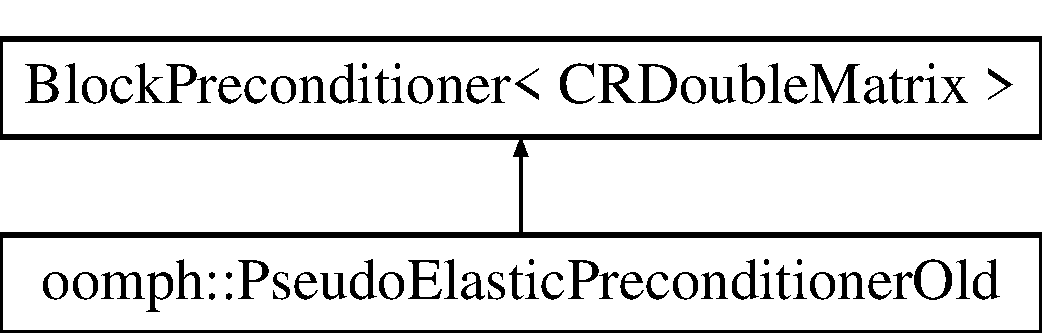
\includegraphics[height=2.000000cm]{classoomph_1_1PseudoElasticPreconditionerOld}
\end{center}
\end{figure}
\subsection*{Public Types}
\begin{DoxyCompactItemize}
\item 
enum \hyperlink{classoomph_1_1PseudoElasticPreconditionerOld_a6748360e3e2fbd4766d837a520dadfd0}{Elastic\+\_\+preconditioner\+\_\+type} \{ \hyperlink{classoomph_1_1PseudoElasticPreconditionerOld_a6748360e3e2fbd4766d837a520dadfd0a6715e85e01ea15dda633e9752d1b2df4}{Exact\+\_\+block\+\_\+preconditioner}, 
\hyperlink{classoomph_1_1PseudoElasticPreconditionerOld_a6748360e3e2fbd4766d837a520dadfd0ab93e9663b3ce2d96ceb2f48b99802120}{Block\+\_\+diagonal\+\_\+preconditioner}, 
\hyperlink{classoomph_1_1PseudoElasticPreconditionerOld_a6748360e3e2fbd4766d837a520dadfd0a89ac82b79943728045e50d6d2a17a27b}{Block\+\_\+lower\+\_\+triangular\+\_\+preconditioner}, 
\hyperlink{classoomph_1_1PseudoElasticPreconditionerOld_a6748360e3e2fbd4766d837a520dadfd0a7faa51d91917bad39dbc2e27b9af7bbc}{Block\+\_\+upper\+\_\+triangular\+\_\+preconditioner}
 \}\begin{DoxyCompactList}\small\item\em The augmented elasticity system can be preconditioned in one of four ways. 0 -\/ Exact preconditioner 1 -\/ Block diagonal preconditioning 2 -\/ Block upper triangular preconditioner 3 -\/ Block lower triangular preconditioner We group together the different components of the displacement vector field for the block decomposition. \end{DoxyCompactList}
\item 
typedef Preconditioner $\ast$($\ast$ \hyperlink{classoomph_1_1PseudoElasticPreconditionerOld_a8ee80a4a55139190a6e2a16fa175e75f}{Subsidiary\+Preconditioner\+Fct\+Pt}) ()
\begin{DoxyCompactList}\small\item\em This preconditioner includes the option to use subsidiary operators other than Super\+L\+U\+Preconditioner for this problem. This is the typedef of a function that should return an instance of a subsidiary preconditioning operator. This preconditioner is responsible for the destruction of the subsidiary preconditioners. \end{DoxyCompactList}\end{DoxyCompactItemize}
\subsection*{Public Member Functions}
\begin{DoxyCompactItemize}
\item 
\hyperlink{classoomph_1_1PseudoElasticPreconditionerOld_a604bb3a8e087574657d28feee1cc2611}{Pseudo\+Elastic\+Preconditioner\+Old} ()
\begin{DoxyCompactList}\small\item\em Default (and only) constructor. \end{DoxyCompactList}\item 
virtual \hyperlink{classoomph_1_1PseudoElasticPreconditionerOld_a1e690693abc957640c99b63fe3c5c73f}{$\sim$\+Pseudo\+Elastic\+Preconditioner\+Old} ()
\begin{DoxyCompactList}\small\item\em destructor \end{DoxyCompactList}\item 
\hyperlink{classoomph_1_1PseudoElasticPreconditionerOld_a8186e3328b5b93186645812e79324843}{Pseudo\+Elastic\+Preconditioner\+Old} (const \hyperlink{classoomph_1_1PseudoElasticPreconditionerOld}{Pseudo\+Elastic\+Preconditioner\+Old} \&)
\begin{DoxyCompactList}\small\item\em Broken copy constructor. \end{DoxyCompactList}\item 
void \hyperlink{classoomph_1_1PseudoElasticPreconditionerOld_a25d542a5b98d70be1aa1dd6000402978}{setup} ()
\begin{DoxyCompactList}\small\item\em Broken assignment operator. \end{DoxyCompactList}\item 
void \hyperlink{classoomph_1_1PseudoElasticPreconditionerOld_a20b548d07e0f4116f59444ccb69d980f}{preconditioner\+\_\+solve} (const Double\+Vector \&r, Double\+Vector \&z)
\begin{DoxyCompactList}\small\item\em Apply the preconditioner. Method implemented in two other methods (elastic and lagrange multiplier subsidiary preocnditioner) for the \hyperlink{classoomph_1_1PseudoElasticFSIPreconditioner}{Pseudo\+Elastic\+F\+S\+I\+Preconditioner}. \end{DoxyCompactList}\item 
void \hyperlink{classoomph_1_1PseudoElasticPreconditionerOld_a96464001afad81606a6d298f4045de70}{set\+\_\+elastic\+\_\+mesh} (Mesh $\ast$mesh\+\_\+pt)
\begin{DoxyCompactList}\small\item\em Access function to mesh containing the block-\/preconditionable elastic elements. \end{DoxyCompactList}\item 
void \hyperlink{classoomph_1_1PseudoElasticPreconditionerOld_a432b5e0501644ae3fa6a9dadd8f52c60}{set\+\_\+lagrange\+\_\+multiplier\+\_\+mesh} (Mesh $\ast$mesh\+\_\+pt)
\begin{DoxyCompactList}\small\item\em Access function to mesh containing the block-\/preconditionable lagrange multiplier elements. \end{DoxyCompactList}\item 
void \hyperlink{classoomph_1_1PseudoElasticPreconditionerOld_a5175c5ba92a63e7e47ca87883753b28c}{enable\+\_\+inf\+\_\+norm\+\_\+of\+\_\+s\+\_\+scaling} ()
\begin{DoxyCompactList}\small\item\em Call to use the inf norm of S as scaling. \end{DoxyCompactList}\item 
void \hyperlink{classoomph_1_1PseudoElasticPreconditionerOld_a5b23f319564110f34c07fbaacd40e446}{disable\+\_\+inf\+\_\+norm\+\_\+of\+\_\+s\+\_\+scaling} ()
\begin{DoxyCompactList}\small\item\em Call to use no scaling. \end{DoxyCompactList}\item 
void \hyperlink{classoomph_1_1PseudoElasticPreconditionerOld_ab0f5cd103d172fcb33be52c17bb741d3}{set\+\_\+lagrange\+\_\+multiplier\+\_\+subsidiary\+\_\+preconditioner} (\hyperlink{classoomph_1_1PseudoElasticPreconditionerOld_a8ee80a4a55139190a6e2a16fa175e75f}{Subsidiary\+Preconditioner\+Fct\+Pt} prec\+\_\+fn)
\begin{DoxyCompactList}\small\item\em By default the Lagrange multiplier subsidiary systems are preconditioner with Super\+L\+U\+Preconditioner. For a different preconditioner, pass a function to this method returning a different subsidiary operator. \end{DoxyCompactList}\item 
void \hyperlink{classoomph_1_1PseudoElasticPreconditionerOld_aae1c5f984fee69fca7cd9719ed2222a4}{set\+\_\+elastic\+\_\+subsidiary\+\_\+preconditioner} (\hyperlink{classoomph_1_1PseudoElasticPreconditionerOld_a8ee80a4a55139190a6e2a16fa175e75f}{Subsidiary\+Preconditioner\+Fct\+Pt} prec\+\_\+fn)
\begin{DoxyCompactList}\small\item\em By default the elastic subsidiary systems are preconditioner with Super\+L\+U\+Preconditioner. For a different preconditioner, pass a function to this method returning a different subsidiary operator. \end{DoxyCompactList}\item 
\hyperlink{classoomph_1_1PseudoElasticPreconditionerOld_a6748360e3e2fbd4766d837a520dadfd0}{Elastic\+\_\+preconditioner\+\_\+type} \& \hyperlink{classoomph_1_1PseudoElasticPreconditionerOld_a9edf6f556251ea6ca1b15baf3f6b0425}{elastic\+\_\+preconditioner\+\_\+type} ()
\begin{DoxyCompactList}\small\item\em Set the type of preconditioner applied to the elastic\+: 0 -\/ Exact preconditioner 1 -\/ Block diagonal preconditioning 2 -\/ Block upper triangular preconditioner 3 -\/ Block lower triangular preconditioner We group together the different components of the displacement vector field for the block decomposition. \end{DoxyCompactList}\item 
void \hyperlink{classoomph_1_1PseudoElasticPreconditionerOld_acadd6682a6d25534d7e2be1e95c4d0e6}{clean\+\_\+up\+\_\+memory} ()
\begin{DoxyCompactList}\small\item\em Clears the memory. \end{DoxyCompactList}\end{DoxyCompactItemize}
\subsection*{Private Member Functions}
\begin{DoxyCompactItemize}
\item 
void \hyperlink{classoomph_1_1PseudoElasticPreconditionerOld_a5255c2de35cb38cd49e71220e96db22c}{elastic\+\_\+preconditioner\+\_\+solve} (const Double\+Vector \&r, Double\+Vector \&z)
\begin{DoxyCompactList}\small\item\em Apply the elastic subsidiary preconditioner. \end{DoxyCompactList}\item 
void \hyperlink{classoomph_1_1PseudoElasticPreconditionerOld_a02d8d2a2ad34030238f7f65964f91a08}{lagrange\+\_\+multiplier\+\_\+preconditioner\+\_\+solve} (const Double\+Vector \&r, Double\+Vector \&z)
\begin{DoxyCompactList}\small\item\em Apply the lagrange multiplier subsidiary preconditioner. \end{DoxyCompactList}\end{DoxyCompactItemize}
\subsection*{Private Attributes}
\begin{DoxyCompactItemize}
\item 
double \hyperlink{classoomph_1_1PseudoElasticPreconditionerOld_a563f753bed7b33a169ec15b796864eba}{Scaling}
\begin{DoxyCompactList}\small\item\em The scaling. Defaults to infinity norm of S. \end{DoxyCompactList}\item 
bool \hyperlink{classoomph_1_1PseudoElasticPreconditionerOld_a475f2a2576128e4a17ee494343438ba5}{Use\+\_\+inf\+\_\+norm\+\_\+of\+\_\+s\+\_\+scaling}
\begin{DoxyCompactList}\small\item\em boolean indicating whether the inf-\/norm of S should be used as scaling. Default = true; \end{DoxyCompactList}\item 
\hyperlink{classoomph_1_1PseudoElasticPreconditionerOld_a6748360e3e2fbd4766d837a520dadfd0}{Elastic\+\_\+preconditioner\+\_\+type} \hyperlink{classoomph_1_1PseudoElasticPreconditionerOld_a4cb348ca052099063282dc8adb76d5fc}{E\+\_\+preconditioner\+\_\+type}
\begin{DoxyCompactList}\small\item\em An unsigned indicating which method should be used for preconditioning the solid component. \end{DoxyCompactList}\item 
unsigned \hyperlink{classoomph_1_1PseudoElasticPreconditionerOld_a61d6f0e7db9902aa2bde14bfdf933bae}{Dim}
\begin{DoxyCompactList}\small\item\em the dimension of the problem \end{DoxyCompactList}\item 
Preconditioner $\ast$ \hyperlink{classoomph_1_1PseudoElasticPreconditionerOld_a14f587c9c01c392b14c235bde00453b3}{Elastic\+\_\+preconditioner\+\_\+pt}
\begin{DoxyCompactList}\small\item\em storage for the preconditioner for the solid system \end{DoxyCompactList}\item 
Vector$<$ Preconditioner $\ast$ $>$ \hyperlink{classoomph_1_1PseudoElasticPreconditionerOld_a14f5c801cd3c9128705902002efe51e8}{Lagrange\+\_\+multiplier\+\_\+preconditioner\+\_\+pt}
\begin{DoxyCompactList}\small\item\em lagrange multiplier preconditioner pt \end{DoxyCompactList}\item 
\hyperlink{classoomph_1_1PseudoElasticPreconditionerOld_a8ee80a4a55139190a6e2a16fa175e75f}{Subsidiary\+Preconditioner\+Fct\+Pt} \hyperlink{classoomph_1_1PseudoElasticPreconditionerOld_ab010ad3548eec31d287215c63aad1abe}{Lagrange\+\_\+multiplier\+\_\+subsidiary\+\_\+preconditioner\+\_\+function\+\_\+pt}
\begin{DoxyCompactList}\small\item\em The Lagrange multiplier subsidary preconditioner function pointer. \end{DoxyCompactList}\item 
\hyperlink{classoomph_1_1PseudoElasticPreconditionerOld_a8ee80a4a55139190a6e2a16fa175e75f}{Subsidiary\+Preconditioner\+Fct\+Pt} \hyperlink{classoomph_1_1PseudoElasticPreconditionerOld_a48a6c1d213cabb8849b6abcad8415152}{Elastic\+\_\+subsidiary\+\_\+preconditioner\+\_\+function\+\_\+pt}
\begin{DoxyCompactList}\small\item\em The solid subsidiary preconditioner function pointer. \end{DoxyCompactList}\item 
Mesh $\ast$ \hyperlink{classoomph_1_1PseudoElasticPreconditionerOld_ab45147d893d104fbf3c0ebc0bacafc7d}{Elastic\+\_\+mesh\+\_\+pt}
\begin{DoxyCompactList}\small\item\em Pointer to the mesh containing the solid elements. \end{DoxyCompactList}\item 
Mesh $\ast$ \hyperlink{classoomph_1_1PseudoElasticPreconditionerOld_aee91427e4d8d57802728291d8576d5a4}{Lagrange\+\_\+multiplier\+\_\+mesh\+\_\+pt}
\begin{DoxyCompactList}\small\item\em Pointer to the mesh containing the Lagrange multiplier elements. \end{DoxyCompactList}\end{DoxyCompactItemize}
\subsection*{Friends}
\begin{DoxyCompactItemize}
\item 
class \hyperlink{classoomph_1_1PseudoElasticPreconditionerOld_aaaea2b4795566f81945597254305249d}{Pseudo\+Elastic\+F\+S\+I\+Preconditioner}
\begin{DoxyCompactList}\small\item\em \hyperlink{classoomph_1_1PseudoElasticFSIPreconditioner}{Pseudo\+Elastic\+F\+S\+I\+Preconditioner} is a friend to access the private $\ast$\+\_\+preconditioner\+\_\+solve(...) method. \end{DoxyCompactList}\end{DoxyCompactItemize}


\subsection{Detailed Description}
A subsidiary preconditioner for the pseudo-\/elastic F\+SI preconditioner. Also a stand-\/alone preconditioner for the problem of non-\/linear elasticity subject to prescribed displacement by Lagrange multiplier.. {\bfseries Enumeration} of Elastic D\+OF types in the Pseudo-\/\+Elastic Elements The method get\+\_\+dof\+\_\+types\+\_\+for\+\_\+unknowns() must be implemented such that D\+O\+Fs subject be Lagrange multiplier and D\+O\+Fs N\+OT subject to Lagrange multiplier have different labels. For example in a 3D problem there are 6 D\+OF types and the following labelling must be implemented\+: 0 -\/ x displacement (without lagr mult traction) 1 -\/ y displacement (without lagr mult traction) 2 -\/ z displacement (without lagr mult traction) 4 -\/ x displacement (with lagr mult traction) 5 -\/ y displacement (with lagr mult traction) 6 -\/ z displacement (with lagr mult traction) 

Definition at line 312 of file pseudo\+\_\+elastic\+\_\+preconditioner.\+h.



\subsection{Member Typedef Documentation}
\mbox{\Hypertarget{classoomph_1_1PseudoElasticPreconditionerOld_a8ee80a4a55139190a6e2a16fa175e75f}\label{classoomph_1_1PseudoElasticPreconditionerOld_a8ee80a4a55139190a6e2a16fa175e75f}} 
\index{oomph\+::\+Pseudo\+Elastic\+Preconditioner\+Old@{oomph\+::\+Pseudo\+Elastic\+Preconditioner\+Old}!Subsidiary\+Preconditioner\+Fct\+Pt@{Subsidiary\+Preconditioner\+Fct\+Pt}}
\index{Subsidiary\+Preconditioner\+Fct\+Pt@{Subsidiary\+Preconditioner\+Fct\+Pt}!oomph\+::\+Pseudo\+Elastic\+Preconditioner\+Old@{oomph\+::\+Pseudo\+Elastic\+Preconditioner\+Old}}
\subsubsection{\texorpdfstring{Subsidiary\+Preconditioner\+Fct\+Pt}{SubsidiaryPreconditionerFctPt}}
{\footnotesize\ttfamily typedef Preconditioner$\ast$($\ast$ oomph\+::\+Pseudo\+Elastic\+Preconditioner\+Old\+::\+Subsidiary\+Preconditioner\+Fct\+Pt) ()}



This preconditioner includes the option to use subsidiary operators other than Super\+L\+U\+Preconditioner for this problem. This is the typedef of a function that should return an instance of a subsidiary preconditioning operator. This preconditioner is responsible for the destruction of the subsidiary preconditioners. 



Definition at line 326 of file pseudo\+\_\+elastic\+\_\+preconditioner.\+h.



\subsection{Member Enumeration Documentation}
\mbox{\Hypertarget{classoomph_1_1PseudoElasticPreconditionerOld_a6748360e3e2fbd4766d837a520dadfd0}\label{classoomph_1_1PseudoElasticPreconditionerOld_a6748360e3e2fbd4766d837a520dadfd0}} 
\index{oomph\+::\+Pseudo\+Elastic\+Preconditioner\+Old@{oomph\+::\+Pseudo\+Elastic\+Preconditioner\+Old}!Elastic\+\_\+preconditioner\+\_\+type@{Elastic\+\_\+preconditioner\+\_\+type}}
\index{Elastic\+\_\+preconditioner\+\_\+type@{Elastic\+\_\+preconditioner\+\_\+type}!oomph\+::\+Pseudo\+Elastic\+Preconditioner\+Old@{oomph\+::\+Pseudo\+Elastic\+Preconditioner\+Old}}
\subsubsection{\texorpdfstring{Elastic\+\_\+preconditioner\+\_\+type}{Elastic\_preconditioner\_type}}
{\footnotesize\ttfamily enum \hyperlink{classoomph_1_1PseudoElasticPreconditionerOld_a6748360e3e2fbd4766d837a520dadfd0}{oomph\+::\+Pseudo\+Elastic\+Preconditioner\+Old\+::\+Elastic\+\_\+preconditioner\+\_\+type}}



The augmented elasticity system can be preconditioned in one of four ways. 0 -\/ Exact preconditioner 1 -\/ Block diagonal preconditioning 2 -\/ Block upper triangular preconditioner 3 -\/ Block lower triangular preconditioner We group together the different components of the displacement vector field for the block decomposition. 

\begin{DoxyEnumFields}{Enumerator}
\raisebox{\heightof{T}}[0pt][0pt]{\index{Exact\+\_\+block\+\_\+preconditioner@{Exact\+\_\+block\+\_\+preconditioner}!oomph\+::\+Pseudo\+Elastic\+Preconditioner\+Old@{oomph\+::\+Pseudo\+Elastic\+Preconditioner\+Old}}\index{oomph\+::\+Pseudo\+Elastic\+Preconditioner\+Old@{oomph\+::\+Pseudo\+Elastic\+Preconditioner\+Old}!Exact\+\_\+block\+\_\+preconditioner@{Exact\+\_\+block\+\_\+preconditioner}}}\mbox{\Hypertarget{classoomph_1_1PseudoElasticPreconditionerOld_a6748360e3e2fbd4766d837a520dadfd0a6715e85e01ea15dda633e9752d1b2df4}\label{classoomph_1_1PseudoElasticPreconditionerOld_a6748360e3e2fbd4766d837a520dadfd0a6715e85e01ea15dda633e9752d1b2df4}} 
Exact\+\_\+block\+\_\+preconditioner&\\
\hline

\raisebox{\heightof{T}}[0pt][0pt]{\index{Block\+\_\+diagonal\+\_\+preconditioner@{Block\+\_\+diagonal\+\_\+preconditioner}!oomph\+::\+Pseudo\+Elastic\+Preconditioner\+Old@{oomph\+::\+Pseudo\+Elastic\+Preconditioner\+Old}}\index{oomph\+::\+Pseudo\+Elastic\+Preconditioner\+Old@{oomph\+::\+Pseudo\+Elastic\+Preconditioner\+Old}!Block\+\_\+diagonal\+\_\+preconditioner@{Block\+\_\+diagonal\+\_\+preconditioner}}}\mbox{\Hypertarget{classoomph_1_1PseudoElasticPreconditionerOld_a6748360e3e2fbd4766d837a520dadfd0ab93e9663b3ce2d96ceb2f48b99802120}\label{classoomph_1_1PseudoElasticPreconditionerOld_a6748360e3e2fbd4766d837a520dadfd0ab93e9663b3ce2d96ceb2f48b99802120}} 
Block\+\_\+diagonal\+\_\+preconditioner&\\
\hline

\raisebox{\heightof{T}}[0pt][0pt]{\index{Block\+\_\+lower\+\_\+triangular\+\_\+preconditioner@{Block\+\_\+lower\+\_\+triangular\+\_\+preconditioner}!oomph\+::\+Pseudo\+Elastic\+Preconditioner\+Old@{oomph\+::\+Pseudo\+Elastic\+Preconditioner\+Old}}\index{oomph\+::\+Pseudo\+Elastic\+Preconditioner\+Old@{oomph\+::\+Pseudo\+Elastic\+Preconditioner\+Old}!Block\+\_\+lower\+\_\+triangular\+\_\+preconditioner@{Block\+\_\+lower\+\_\+triangular\+\_\+preconditioner}}}\mbox{\Hypertarget{classoomph_1_1PseudoElasticPreconditionerOld_a6748360e3e2fbd4766d837a520dadfd0a89ac82b79943728045e50d6d2a17a27b}\label{classoomph_1_1PseudoElasticPreconditionerOld_a6748360e3e2fbd4766d837a520dadfd0a89ac82b79943728045e50d6d2a17a27b}} 
Block\+\_\+lower\+\_\+triangular\+\_\+preconditioner&\\
\hline

\raisebox{\heightof{T}}[0pt][0pt]{\index{Block\+\_\+upper\+\_\+triangular\+\_\+preconditioner@{Block\+\_\+upper\+\_\+triangular\+\_\+preconditioner}!oomph\+::\+Pseudo\+Elastic\+Preconditioner\+Old@{oomph\+::\+Pseudo\+Elastic\+Preconditioner\+Old}}\index{oomph\+::\+Pseudo\+Elastic\+Preconditioner\+Old@{oomph\+::\+Pseudo\+Elastic\+Preconditioner\+Old}!Block\+\_\+upper\+\_\+triangular\+\_\+preconditioner@{Block\+\_\+upper\+\_\+triangular\+\_\+preconditioner}}}\mbox{\Hypertarget{classoomph_1_1PseudoElasticPreconditionerOld_a6748360e3e2fbd4766d837a520dadfd0a7faa51d91917bad39dbc2e27b9af7bbc}\label{classoomph_1_1PseudoElasticPreconditionerOld_a6748360e3e2fbd4766d837a520dadfd0a7faa51d91917bad39dbc2e27b9af7bbc}} 
Block\+\_\+upper\+\_\+triangular\+\_\+preconditioner&\\
\hline

\end{DoxyEnumFields}


Definition at line 336 of file pseudo\+\_\+elastic\+\_\+preconditioner.\+h.



\subsection{Constructor \& Destructor Documentation}
\mbox{\Hypertarget{classoomph_1_1PseudoElasticPreconditionerOld_a604bb3a8e087574657d28feee1cc2611}\label{classoomph_1_1PseudoElasticPreconditionerOld_a604bb3a8e087574657d28feee1cc2611}} 
\index{oomph\+::\+Pseudo\+Elastic\+Preconditioner\+Old@{oomph\+::\+Pseudo\+Elastic\+Preconditioner\+Old}!Pseudo\+Elastic\+Preconditioner\+Old@{Pseudo\+Elastic\+Preconditioner\+Old}}
\index{Pseudo\+Elastic\+Preconditioner\+Old@{Pseudo\+Elastic\+Preconditioner\+Old}!oomph\+::\+Pseudo\+Elastic\+Preconditioner\+Old@{oomph\+::\+Pseudo\+Elastic\+Preconditioner\+Old}}
\subsubsection{\texorpdfstring{Pseudo\+Elastic\+Preconditioner\+Old()}{PseudoElasticPreconditionerOld()}\hspace{0.1cm}{\footnotesize\ttfamily [1/2]}}
{\footnotesize\ttfamily oomph\+::\+Pseudo\+Elastic\+Preconditioner\+Old\+::\+Pseudo\+Elastic\+Preconditioner\+Old (\begin{DoxyParamCaption}{ }\end{DoxyParamCaption})\hspace{0.3cm}{\ttfamily [inline]}}



Default (and only) constructor. 



Definition at line 342 of file pseudo\+\_\+elastic\+\_\+preconditioner.\+h.

\mbox{\Hypertarget{classoomph_1_1PseudoElasticPreconditionerOld_a1e690693abc957640c99b63fe3c5c73f}\label{classoomph_1_1PseudoElasticPreconditionerOld_a1e690693abc957640c99b63fe3c5c73f}} 
\index{oomph\+::\+Pseudo\+Elastic\+Preconditioner\+Old@{oomph\+::\+Pseudo\+Elastic\+Preconditioner\+Old}!````~Pseudo\+Elastic\+Preconditioner\+Old@{$\sim$\+Pseudo\+Elastic\+Preconditioner\+Old}}
\index{````~Pseudo\+Elastic\+Preconditioner\+Old@{$\sim$\+Pseudo\+Elastic\+Preconditioner\+Old}!oomph\+::\+Pseudo\+Elastic\+Preconditioner\+Old@{oomph\+::\+Pseudo\+Elastic\+Preconditioner\+Old}}
\subsubsection{\texorpdfstring{$\sim$\+Pseudo\+Elastic\+Preconditioner\+Old()}{~PseudoElasticPreconditionerOld()}}
{\footnotesize\ttfamily virtual oomph\+::\+Pseudo\+Elastic\+Preconditioner\+Old\+::$\sim$\+Pseudo\+Elastic\+Preconditioner\+Old (\begin{DoxyParamCaption}{ }\end{DoxyParamCaption})\hspace{0.3cm}{\ttfamily [inline]}, {\ttfamily [virtual]}}



destructor 



Definition at line 359 of file pseudo\+\_\+elastic\+\_\+preconditioner.\+h.

\mbox{\Hypertarget{classoomph_1_1PseudoElasticPreconditionerOld_a8186e3328b5b93186645812e79324843}\label{classoomph_1_1PseudoElasticPreconditionerOld_a8186e3328b5b93186645812e79324843}} 
\index{oomph\+::\+Pseudo\+Elastic\+Preconditioner\+Old@{oomph\+::\+Pseudo\+Elastic\+Preconditioner\+Old}!Pseudo\+Elastic\+Preconditioner\+Old@{Pseudo\+Elastic\+Preconditioner\+Old}}
\index{Pseudo\+Elastic\+Preconditioner\+Old@{Pseudo\+Elastic\+Preconditioner\+Old}!oomph\+::\+Pseudo\+Elastic\+Preconditioner\+Old@{oomph\+::\+Pseudo\+Elastic\+Preconditioner\+Old}}
\subsubsection{\texorpdfstring{Pseudo\+Elastic\+Preconditioner\+Old()}{PseudoElasticPreconditionerOld()}\hspace{0.1cm}{\footnotesize\ttfamily [2/2]}}
{\footnotesize\ttfamily oomph\+::\+Pseudo\+Elastic\+Preconditioner\+Old\+::\+Pseudo\+Elastic\+Preconditioner\+Old (\begin{DoxyParamCaption}\item[{const \hyperlink{classoomph_1_1PseudoElasticPreconditionerOld}{Pseudo\+Elastic\+Preconditioner\+Old} \&}]{ }\end{DoxyParamCaption})\hspace{0.3cm}{\ttfamily [inline]}}



Broken copy constructor. 



Definition at line 366 of file pseudo\+\_\+elastic\+\_\+preconditioner.\+h.



\subsection{Member Function Documentation}
\mbox{\Hypertarget{classoomph_1_1PseudoElasticPreconditionerOld_acadd6682a6d25534d7e2be1e95c4d0e6}\label{classoomph_1_1PseudoElasticPreconditionerOld_acadd6682a6d25534d7e2be1e95c4d0e6}} 
\index{oomph\+::\+Pseudo\+Elastic\+Preconditioner\+Old@{oomph\+::\+Pseudo\+Elastic\+Preconditioner\+Old}!clean\+\_\+up\+\_\+memory@{clean\+\_\+up\+\_\+memory}}
\index{clean\+\_\+up\+\_\+memory@{clean\+\_\+up\+\_\+memory}!oomph\+::\+Pseudo\+Elastic\+Preconditioner\+Old@{oomph\+::\+Pseudo\+Elastic\+Preconditioner\+Old}}
\subsubsection{\texorpdfstring{clean\+\_\+up\+\_\+memory()}{clean\_up\_memory()}}
{\footnotesize\ttfamily void oomph\+::\+Pseudo\+Elastic\+Preconditioner\+Old\+::clean\+\_\+up\+\_\+memory (\begin{DoxyParamCaption}{ }\end{DoxyParamCaption})}



Clears the memory. 



Definition at line 808 of file pseudo\+\_\+elastic\+\_\+preconditioner.\+cc.



References oomph\+::\+Pseudo\+Elastic\+Preconditioner\+Subsidiary\+Preconditioner\+Old\+::setup().

\mbox{\Hypertarget{classoomph_1_1PseudoElasticPreconditionerOld_a5b23f319564110f34c07fbaacd40e446}\label{classoomph_1_1PseudoElasticPreconditionerOld_a5b23f319564110f34c07fbaacd40e446}} 
\index{oomph\+::\+Pseudo\+Elastic\+Preconditioner\+Old@{oomph\+::\+Pseudo\+Elastic\+Preconditioner\+Old}!disable\+\_\+inf\+\_\+norm\+\_\+of\+\_\+s\+\_\+scaling@{disable\+\_\+inf\+\_\+norm\+\_\+of\+\_\+s\+\_\+scaling}}
\index{disable\+\_\+inf\+\_\+norm\+\_\+of\+\_\+s\+\_\+scaling@{disable\+\_\+inf\+\_\+norm\+\_\+of\+\_\+s\+\_\+scaling}!oomph\+::\+Pseudo\+Elastic\+Preconditioner\+Old@{oomph\+::\+Pseudo\+Elastic\+Preconditioner\+Old}}
\subsubsection{\texorpdfstring{disable\+\_\+inf\+\_\+norm\+\_\+of\+\_\+s\+\_\+scaling()}{disable\_inf\_norm\_of\_s\_scaling()}}
{\footnotesize\ttfamily void oomph\+::\+Pseudo\+Elastic\+Preconditioner\+Old\+::disable\+\_\+inf\+\_\+norm\+\_\+of\+\_\+s\+\_\+scaling (\begin{DoxyParamCaption}{ }\end{DoxyParamCaption})\hspace{0.3cm}{\ttfamily [inline]}}



Call to use no scaling. 



Definition at line 409 of file pseudo\+\_\+elastic\+\_\+preconditioner.\+h.

\mbox{\Hypertarget{classoomph_1_1PseudoElasticPreconditionerOld_a5255c2de35cb38cd49e71220e96db22c}\label{classoomph_1_1PseudoElasticPreconditionerOld_a5255c2de35cb38cd49e71220e96db22c}} 
\index{oomph\+::\+Pseudo\+Elastic\+Preconditioner\+Old@{oomph\+::\+Pseudo\+Elastic\+Preconditioner\+Old}!elastic\+\_\+preconditioner\+\_\+solve@{elastic\+\_\+preconditioner\+\_\+solve}}
\index{elastic\+\_\+preconditioner\+\_\+solve@{elastic\+\_\+preconditioner\+\_\+solve}!oomph\+::\+Pseudo\+Elastic\+Preconditioner\+Old@{oomph\+::\+Pseudo\+Elastic\+Preconditioner\+Old}}
\subsubsection{\texorpdfstring{elastic\+\_\+preconditioner\+\_\+solve()}{elastic\_preconditioner\_solve()}}
{\footnotesize\ttfamily void oomph\+::\+Pseudo\+Elastic\+Preconditioner\+Old\+::elastic\+\_\+preconditioner\+\_\+solve (\begin{DoxyParamCaption}\item[{const Double\+Vector \&}]{r,  }\item[{Double\+Vector \&}]{z }\end{DoxyParamCaption})\hspace{0.3cm}{\ttfamily [private]}}



Apply the elastic subsidiary preconditioner. 



Definition at line 773 of file pseudo\+\_\+elastic\+\_\+preconditioner.\+cc.



References lagrange\+\_\+multiplier\+\_\+preconditioner\+\_\+solve().



Referenced by setup().

\mbox{\Hypertarget{classoomph_1_1PseudoElasticPreconditionerOld_a9edf6f556251ea6ca1b15baf3f6b0425}\label{classoomph_1_1PseudoElasticPreconditionerOld_a9edf6f556251ea6ca1b15baf3f6b0425}} 
\index{oomph\+::\+Pseudo\+Elastic\+Preconditioner\+Old@{oomph\+::\+Pseudo\+Elastic\+Preconditioner\+Old}!elastic\+\_\+preconditioner\+\_\+type@{elastic\+\_\+preconditioner\+\_\+type}}
\index{elastic\+\_\+preconditioner\+\_\+type@{elastic\+\_\+preconditioner\+\_\+type}!oomph\+::\+Pseudo\+Elastic\+Preconditioner\+Old@{oomph\+::\+Pseudo\+Elastic\+Preconditioner\+Old}}
\subsubsection{\texorpdfstring{elastic\+\_\+preconditioner\+\_\+type()}{elastic\_preconditioner\_type()}}
{\footnotesize\ttfamily \hyperlink{classoomph_1_1PseudoElasticPreconditionerOld_a6748360e3e2fbd4766d837a520dadfd0}{Elastic\+\_\+preconditioner\+\_\+type}\& oomph\+::\+Pseudo\+Elastic\+Preconditioner\+Old\+::elastic\+\_\+preconditioner\+\_\+type (\begin{DoxyParamCaption}{ }\end{DoxyParamCaption})\hspace{0.3cm}{\ttfamily [inline]}}



Set the type of preconditioner applied to the elastic\+: 0 -\/ Exact preconditioner 1 -\/ Block diagonal preconditioning 2 -\/ Block upper triangular preconditioner 3 -\/ Block lower triangular preconditioner We group together the different components of the displacement vector field for the block decomposition. 



Definition at line 439 of file pseudo\+\_\+elastic\+\_\+preconditioner.\+h.

\mbox{\Hypertarget{classoomph_1_1PseudoElasticPreconditionerOld_a5175c5ba92a63e7e47ca87883753b28c}\label{classoomph_1_1PseudoElasticPreconditionerOld_a5175c5ba92a63e7e47ca87883753b28c}} 
\index{oomph\+::\+Pseudo\+Elastic\+Preconditioner\+Old@{oomph\+::\+Pseudo\+Elastic\+Preconditioner\+Old}!enable\+\_\+inf\+\_\+norm\+\_\+of\+\_\+s\+\_\+scaling@{enable\+\_\+inf\+\_\+norm\+\_\+of\+\_\+s\+\_\+scaling}}
\index{enable\+\_\+inf\+\_\+norm\+\_\+of\+\_\+s\+\_\+scaling@{enable\+\_\+inf\+\_\+norm\+\_\+of\+\_\+s\+\_\+scaling}!oomph\+::\+Pseudo\+Elastic\+Preconditioner\+Old@{oomph\+::\+Pseudo\+Elastic\+Preconditioner\+Old}}
\subsubsection{\texorpdfstring{enable\+\_\+inf\+\_\+norm\+\_\+of\+\_\+s\+\_\+scaling()}{enable\_inf\_norm\_of\_s\_scaling()}}
{\footnotesize\ttfamily void oomph\+::\+Pseudo\+Elastic\+Preconditioner\+Old\+::enable\+\_\+inf\+\_\+norm\+\_\+of\+\_\+s\+\_\+scaling (\begin{DoxyParamCaption}{ }\end{DoxyParamCaption})\hspace{0.3cm}{\ttfamily [inline]}}



Call to use the inf norm of S as scaling. 



Definition at line 405 of file pseudo\+\_\+elastic\+\_\+preconditioner.\+h.

\mbox{\Hypertarget{classoomph_1_1PseudoElasticPreconditionerOld_a02d8d2a2ad34030238f7f65964f91a08}\label{classoomph_1_1PseudoElasticPreconditionerOld_a02d8d2a2ad34030238f7f65964f91a08}} 
\index{oomph\+::\+Pseudo\+Elastic\+Preconditioner\+Old@{oomph\+::\+Pseudo\+Elastic\+Preconditioner\+Old}!lagrange\+\_\+multiplier\+\_\+preconditioner\+\_\+solve@{lagrange\+\_\+multiplier\+\_\+preconditioner\+\_\+solve}}
\index{lagrange\+\_\+multiplier\+\_\+preconditioner\+\_\+solve@{lagrange\+\_\+multiplier\+\_\+preconditioner\+\_\+solve}!oomph\+::\+Pseudo\+Elastic\+Preconditioner\+Old@{oomph\+::\+Pseudo\+Elastic\+Preconditioner\+Old}}
\subsubsection{\texorpdfstring{lagrange\+\_\+multiplier\+\_\+preconditioner\+\_\+solve()}{lagrange\_multiplier\_preconditioner\_solve()}}
{\footnotesize\ttfamily void oomph\+::\+Pseudo\+Elastic\+Preconditioner\+Old\+::lagrange\+\_\+multiplier\+\_\+preconditioner\+\_\+solve (\begin{DoxyParamCaption}\item[{const Double\+Vector \&}]{r,  }\item[{Double\+Vector \&}]{z }\end{DoxyParamCaption})\hspace{0.3cm}{\ttfamily [private]}}



Apply the lagrange multiplier subsidiary preconditioner. 



Definition at line 784 of file pseudo\+\_\+elastic\+\_\+preconditioner.\+cc.



Referenced by elastic\+\_\+preconditioner\+\_\+solve().

\mbox{\Hypertarget{classoomph_1_1PseudoElasticPreconditionerOld_a20b548d07e0f4116f59444ccb69d980f}\label{classoomph_1_1PseudoElasticPreconditionerOld_a20b548d07e0f4116f59444ccb69d980f}} 
\index{oomph\+::\+Pseudo\+Elastic\+Preconditioner\+Old@{oomph\+::\+Pseudo\+Elastic\+Preconditioner\+Old}!preconditioner\+\_\+solve@{preconditioner\+\_\+solve}}
\index{preconditioner\+\_\+solve@{preconditioner\+\_\+solve}!oomph\+::\+Pseudo\+Elastic\+Preconditioner\+Old@{oomph\+::\+Pseudo\+Elastic\+Preconditioner\+Old}}
\subsubsection{\texorpdfstring{preconditioner\+\_\+solve()}{preconditioner\_solve()}}
{\footnotesize\ttfamily void oomph\+::\+Pseudo\+Elastic\+Preconditioner\+Old\+::preconditioner\+\_\+solve (\begin{DoxyParamCaption}\item[{const Double\+Vector \&}]{r,  }\item[{Double\+Vector \&}]{z }\end{DoxyParamCaption})\hspace{0.3cm}{\ttfamily [inline]}}



Apply the preconditioner. Method implemented in two other methods (elastic and lagrange multiplier subsidiary preocnditioner) for the \hyperlink{classoomph_1_1PseudoElasticFSIPreconditioner}{Pseudo\+Elastic\+F\+S\+I\+Preconditioner}. 



Definition at line 384 of file pseudo\+\_\+elastic\+\_\+preconditioner.\+h.

\mbox{\Hypertarget{classoomph_1_1PseudoElasticPreconditionerOld_a96464001afad81606a6d298f4045de70}\label{classoomph_1_1PseudoElasticPreconditionerOld_a96464001afad81606a6d298f4045de70}} 
\index{oomph\+::\+Pseudo\+Elastic\+Preconditioner\+Old@{oomph\+::\+Pseudo\+Elastic\+Preconditioner\+Old}!set\+\_\+elastic\+\_\+mesh@{set\+\_\+elastic\+\_\+mesh}}
\index{set\+\_\+elastic\+\_\+mesh@{set\+\_\+elastic\+\_\+mesh}!oomph\+::\+Pseudo\+Elastic\+Preconditioner\+Old@{oomph\+::\+Pseudo\+Elastic\+Preconditioner\+Old}}
\subsubsection{\texorpdfstring{set\+\_\+elastic\+\_\+mesh()}{set\_elastic\_mesh()}}
{\footnotesize\ttfamily void oomph\+::\+Pseudo\+Elastic\+Preconditioner\+Old\+::set\+\_\+elastic\+\_\+mesh (\begin{DoxyParamCaption}\item[{Mesh $\ast$}]{mesh\+\_\+pt }\end{DoxyParamCaption})\hspace{0.3cm}{\ttfamily [inline]}}



Access function to mesh containing the block-\/preconditionable elastic elements. 



Definition at line 392 of file pseudo\+\_\+elastic\+\_\+preconditioner.\+h.

\mbox{\Hypertarget{classoomph_1_1PseudoElasticPreconditionerOld_aae1c5f984fee69fca7cd9719ed2222a4}\label{classoomph_1_1PseudoElasticPreconditionerOld_aae1c5f984fee69fca7cd9719ed2222a4}} 
\index{oomph\+::\+Pseudo\+Elastic\+Preconditioner\+Old@{oomph\+::\+Pseudo\+Elastic\+Preconditioner\+Old}!set\+\_\+elastic\+\_\+subsidiary\+\_\+preconditioner@{set\+\_\+elastic\+\_\+subsidiary\+\_\+preconditioner}}
\index{set\+\_\+elastic\+\_\+subsidiary\+\_\+preconditioner@{set\+\_\+elastic\+\_\+subsidiary\+\_\+preconditioner}!oomph\+::\+Pseudo\+Elastic\+Preconditioner\+Old@{oomph\+::\+Pseudo\+Elastic\+Preconditioner\+Old}}
\subsubsection{\texorpdfstring{set\+\_\+elastic\+\_\+subsidiary\+\_\+preconditioner()}{set\_elastic\_subsidiary\_preconditioner()}}
{\footnotesize\ttfamily void oomph\+::\+Pseudo\+Elastic\+Preconditioner\+Old\+::set\+\_\+elastic\+\_\+subsidiary\+\_\+preconditioner (\begin{DoxyParamCaption}\item[{\hyperlink{classoomph_1_1PseudoElasticPreconditionerOld_a8ee80a4a55139190a6e2a16fa175e75f}{Subsidiary\+Preconditioner\+Fct\+Pt}}]{prec\+\_\+fn }\end{DoxyParamCaption})\hspace{0.3cm}{\ttfamily [inline]}}



By default the elastic subsidiary systems are preconditioner with Super\+L\+U\+Preconditioner. For a different preconditioner, pass a function to this method returning a different subsidiary operator. 



Definition at line 427 of file pseudo\+\_\+elastic\+\_\+preconditioner.\+h.

\mbox{\Hypertarget{classoomph_1_1PseudoElasticPreconditionerOld_a432b5e0501644ae3fa6a9dadd8f52c60}\label{classoomph_1_1PseudoElasticPreconditionerOld_a432b5e0501644ae3fa6a9dadd8f52c60}} 
\index{oomph\+::\+Pseudo\+Elastic\+Preconditioner\+Old@{oomph\+::\+Pseudo\+Elastic\+Preconditioner\+Old}!set\+\_\+lagrange\+\_\+multiplier\+\_\+mesh@{set\+\_\+lagrange\+\_\+multiplier\+\_\+mesh}}
\index{set\+\_\+lagrange\+\_\+multiplier\+\_\+mesh@{set\+\_\+lagrange\+\_\+multiplier\+\_\+mesh}!oomph\+::\+Pseudo\+Elastic\+Preconditioner\+Old@{oomph\+::\+Pseudo\+Elastic\+Preconditioner\+Old}}
\subsubsection{\texorpdfstring{set\+\_\+lagrange\+\_\+multiplier\+\_\+mesh()}{set\_lagrange\_multiplier\_mesh()}}
{\footnotesize\ttfamily void oomph\+::\+Pseudo\+Elastic\+Preconditioner\+Old\+::set\+\_\+lagrange\+\_\+multiplier\+\_\+mesh (\begin{DoxyParamCaption}\item[{Mesh $\ast$}]{mesh\+\_\+pt }\end{DoxyParamCaption})\hspace{0.3cm}{\ttfamily [inline]}}



Access function to mesh containing the block-\/preconditionable lagrange multiplier elements. 



Definition at line 399 of file pseudo\+\_\+elastic\+\_\+preconditioner.\+h.

\mbox{\Hypertarget{classoomph_1_1PseudoElasticPreconditionerOld_ab0f5cd103d172fcb33be52c17bb741d3}\label{classoomph_1_1PseudoElasticPreconditionerOld_ab0f5cd103d172fcb33be52c17bb741d3}} 
\index{oomph\+::\+Pseudo\+Elastic\+Preconditioner\+Old@{oomph\+::\+Pseudo\+Elastic\+Preconditioner\+Old}!set\+\_\+lagrange\+\_\+multiplier\+\_\+subsidiary\+\_\+preconditioner@{set\+\_\+lagrange\+\_\+multiplier\+\_\+subsidiary\+\_\+preconditioner}}
\index{set\+\_\+lagrange\+\_\+multiplier\+\_\+subsidiary\+\_\+preconditioner@{set\+\_\+lagrange\+\_\+multiplier\+\_\+subsidiary\+\_\+preconditioner}!oomph\+::\+Pseudo\+Elastic\+Preconditioner\+Old@{oomph\+::\+Pseudo\+Elastic\+Preconditioner\+Old}}
\subsubsection{\texorpdfstring{set\+\_\+lagrange\+\_\+multiplier\+\_\+subsidiary\+\_\+preconditioner()}{set\_lagrange\_multiplier\_subsidiary\_preconditioner()}}
{\footnotesize\ttfamily void oomph\+::\+Pseudo\+Elastic\+Preconditioner\+Old\+::set\+\_\+lagrange\+\_\+multiplier\+\_\+subsidiary\+\_\+preconditioner (\begin{DoxyParamCaption}\item[{\hyperlink{classoomph_1_1PseudoElasticPreconditionerOld_a8ee80a4a55139190a6e2a16fa175e75f}{Subsidiary\+Preconditioner\+Fct\+Pt}}]{prec\+\_\+fn }\end{DoxyParamCaption})\hspace{0.3cm}{\ttfamily [inline]}}



By default the Lagrange multiplier subsidiary systems are preconditioner with Super\+L\+U\+Preconditioner. For a different preconditioner, pass a function to this method returning a different subsidiary operator. 



Definition at line 417 of file pseudo\+\_\+elastic\+\_\+preconditioner.\+h.

\mbox{\Hypertarget{classoomph_1_1PseudoElasticPreconditionerOld_a25d542a5b98d70be1aa1dd6000402978}\label{classoomph_1_1PseudoElasticPreconditionerOld_a25d542a5b98d70be1aa1dd6000402978}} 
\index{oomph\+::\+Pseudo\+Elastic\+Preconditioner\+Old@{oomph\+::\+Pseudo\+Elastic\+Preconditioner\+Old}!setup@{setup}}
\index{setup@{setup}!oomph\+::\+Pseudo\+Elastic\+Preconditioner\+Old@{oomph\+::\+Pseudo\+Elastic\+Preconditioner\+Old}}
\subsubsection{\texorpdfstring{setup()}{setup()}}
{\footnotesize\ttfamily void oomph\+::\+Pseudo\+Elastic\+Preconditioner\+Old\+::setup (\begin{DoxyParamCaption}{ }\end{DoxyParamCaption})}



Broken assignment operator. 

Setup method for the \hyperlink{classoomph_1_1PseudoElasticPreconditionerOld}{Pseudo\+Elastic\+Preconditioner\+Old}. 

Definition at line 561 of file pseudo\+\_\+elastic\+\_\+preconditioner.\+cc.



References elastic\+\_\+preconditioner\+\_\+solve(), oomph\+::\+Pseudo\+Elastic\+Preconditioner\+Scaling\+Helper\+Old\+::s\+\_\+inf\+\_\+norm(), oomph\+::\+Pseudo\+Elastic\+Preconditioner\+Subsidiary\+Preconditioner\+Old\+::scaling(), oomph\+::\+Pseudo\+Elastic\+Preconditioner\+Subsidiary\+Block\+Preconditioner\+Old\+::scaling(), oomph\+::\+Pseudo\+Elastic\+Preconditioner\+Subsidiary\+Block\+Preconditioner\+Old\+::use\+\_\+block\+\_\+diagonal\+\_\+approximation(), oomph\+::\+Pseudo\+Elastic\+Preconditioner\+Subsidiary\+Block\+Preconditioner\+Old\+::use\+\_\+lower\+\_\+triangular\+\_\+approximation(), and oomph\+::\+Pseudo\+Elastic\+Preconditioner\+Subsidiary\+Block\+Preconditioner\+Old\+::use\+\_\+upper\+\_\+triangular\+\_\+approximation().



\subsection{Friends And Related Function Documentation}
\mbox{\Hypertarget{classoomph_1_1PseudoElasticPreconditionerOld_aaaea2b4795566f81945597254305249d}\label{classoomph_1_1PseudoElasticPreconditionerOld_aaaea2b4795566f81945597254305249d}} 
\index{oomph\+::\+Pseudo\+Elastic\+Preconditioner\+Old@{oomph\+::\+Pseudo\+Elastic\+Preconditioner\+Old}!Pseudo\+Elastic\+F\+S\+I\+Preconditioner@{Pseudo\+Elastic\+F\+S\+I\+Preconditioner}}
\index{Pseudo\+Elastic\+F\+S\+I\+Preconditioner@{Pseudo\+Elastic\+F\+S\+I\+Preconditioner}!oomph\+::\+Pseudo\+Elastic\+Preconditioner\+Old@{oomph\+::\+Pseudo\+Elastic\+Preconditioner\+Old}}
\subsubsection{\texorpdfstring{Pseudo\+Elastic\+F\+S\+I\+Preconditioner}{PseudoElasticFSIPreconditioner}}
{\footnotesize\ttfamily friend class \hyperlink{classoomph_1_1PseudoElasticFSIPreconditioner}{Pseudo\+Elastic\+F\+S\+I\+Preconditioner}\hspace{0.3cm}{\ttfamily [friend]}}



\hyperlink{classoomph_1_1PseudoElasticFSIPreconditioner}{Pseudo\+Elastic\+F\+S\+I\+Preconditioner} is a friend to access the private $\ast$\+\_\+preconditioner\+\_\+solve(...) method. 



Definition at line 317 of file pseudo\+\_\+elastic\+\_\+preconditioner.\+h.



\subsection{Member Data Documentation}
\mbox{\Hypertarget{classoomph_1_1PseudoElasticPreconditionerOld_a61d6f0e7db9902aa2bde14bfdf933bae}\label{classoomph_1_1PseudoElasticPreconditionerOld_a61d6f0e7db9902aa2bde14bfdf933bae}} 
\index{oomph\+::\+Pseudo\+Elastic\+Preconditioner\+Old@{oomph\+::\+Pseudo\+Elastic\+Preconditioner\+Old}!Dim@{Dim}}
\index{Dim@{Dim}!oomph\+::\+Pseudo\+Elastic\+Preconditioner\+Old@{oomph\+::\+Pseudo\+Elastic\+Preconditioner\+Old}}
\subsubsection{\texorpdfstring{Dim}{Dim}}
{\footnotesize\ttfamily unsigned oomph\+::\+Pseudo\+Elastic\+Preconditioner\+Old\+::\+Dim\hspace{0.3cm}{\ttfamily [private]}}



the dimension of the problem 



Definition at line 468 of file pseudo\+\_\+elastic\+\_\+preconditioner.\+h.

\mbox{\Hypertarget{classoomph_1_1PseudoElasticPreconditionerOld_a4cb348ca052099063282dc8adb76d5fc}\label{classoomph_1_1PseudoElasticPreconditionerOld_a4cb348ca052099063282dc8adb76d5fc}} 
\index{oomph\+::\+Pseudo\+Elastic\+Preconditioner\+Old@{oomph\+::\+Pseudo\+Elastic\+Preconditioner\+Old}!E\+\_\+preconditioner\+\_\+type@{E\+\_\+preconditioner\+\_\+type}}
\index{E\+\_\+preconditioner\+\_\+type@{E\+\_\+preconditioner\+\_\+type}!oomph\+::\+Pseudo\+Elastic\+Preconditioner\+Old@{oomph\+::\+Pseudo\+Elastic\+Preconditioner\+Old}}
\subsubsection{\texorpdfstring{E\+\_\+preconditioner\+\_\+type}{E\_preconditioner\_type}}
{\footnotesize\ttfamily \hyperlink{classoomph_1_1PseudoElasticPreconditionerOld_a6748360e3e2fbd4766d837a520dadfd0}{Elastic\+\_\+preconditioner\+\_\+type} oomph\+::\+Pseudo\+Elastic\+Preconditioner\+Old\+::\+E\+\_\+preconditioner\+\_\+type\hspace{0.3cm}{\ttfamily [private]}}



An unsigned indicating which method should be used for preconditioning the solid component. 



Definition at line 465 of file pseudo\+\_\+elastic\+\_\+preconditioner.\+h.

\mbox{\Hypertarget{classoomph_1_1PseudoElasticPreconditionerOld_ab45147d893d104fbf3c0ebc0bacafc7d}\label{classoomph_1_1PseudoElasticPreconditionerOld_ab45147d893d104fbf3c0ebc0bacafc7d}} 
\index{oomph\+::\+Pseudo\+Elastic\+Preconditioner\+Old@{oomph\+::\+Pseudo\+Elastic\+Preconditioner\+Old}!Elastic\+\_\+mesh\+\_\+pt@{Elastic\+\_\+mesh\+\_\+pt}}
\index{Elastic\+\_\+mesh\+\_\+pt@{Elastic\+\_\+mesh\+\_\+pt}!oomph\+::\+Pseudo\+Elastic\+Preconditioner\+Old@{oomph\+::\+Pseudo\+Elastic\+Preconditioner\+Old}}
\subsubsection{\texorpdfstring{Elastic\+\_\+mesh\+\_\+pt}{Elastic\_mesh\_pt}}
{\footnotesize\ttfamily Mesh$\ast$ oomph\+::\+Pseudo\+Elastic\+Preconditioner\+Old\+::\+Elastic\+\_\+mesh\+\_\+pt\hspace{0.3cm}{\ttfamily [private]}}



Pointer to the mesh containing the solid elements. 



Definition at line 484 of file pseudo\+\_\+elastic\+\_\+preconditioner.\+h.

\mbox{\Hypertarget{classoomph_1_1PseudoElasticPreconditionerOld_a14f587c9c01c392b14c235bde00453b3}\label{classoomph_1_1PseudoElasticPreconditionerOld_a14f587c9c01c392b14c235bde00453b3}} 
\index{oomph\+::\+Pseudo\+Elastic\+Preconditioner\+Old@{oomph\+::\+Pseudo\+Elastic\+Preconditioner\+Old}!Elastic\+\_\+preconditioner\+\_\+pt@{Elastic\+\_\+preconditioner\+\_\+pt}}
\index{Elastic\+\_\+preconditioner\+\_\+pt@{Elastic\+\_\+preconditioner\+\_\+pt}!oomph\+::\+Pseudo\+Elastic\+Preconditioner\+Old@{oomph\+::\+Pseudo\+Elastic\+Preconditioner\+Old}}
\subsubsection{\texorpdfstring{Elastic\+\_\+preconditioner\+\_\+pt}{Elastic\_preconditioner\_pt}}
{\footnotesize\ttfamily Preconditioner$\ast$ oomph\+::\+Pseudo\+Elastic\+Preconditioner\+Old\+::\+Elastic\+\_\+preconditioner\+\_\+pt\hspace{0.3cm}{\ttfamily [private]}}



storage for the preconditioner for the solid system 



Definition at line 471 of file pseudo\+\_\+elastic\+\_\+preconditioner.\+h.

\mbox{\Hypertarget{classoomph_1_1PseudoElasticPreconditionerOld_a48a6c1d213cabb8849b6abcad8415152}\label{classoomph_1_1PseudoElasticPreconditionerOld_a48a6c1d213cabb8849b6abcad8415152}} 
\index{oomph\+::\+Pseudo\+Elastic\+Preconditioner\+Old@{oomph\+::\+Pseudo\+Elastic\+Preconditioner\+Old}!Elastic\+\_\+subsidiary\+\_\+preconditioner\+\_\+function\+\_\+pt@{Elastic\+\_\+subsidiary\+\_\+preconditioner\+\_\+function\+\_\+pt}}
\index{Elastic\+\_\+subsidiary\+\_\+preconditioner\+\_\+function\+\_\+pt@{Elastic\+\_\+subsidiary\+\_\+preconditioner\+\_\+function\+\_\+pt}!oomph\+::\+Pseudo\+Elastic\+Preconditioner\+Old@{oomph\+::\+Pseudo\+Elastic\+Preconditioner\+Old}}
\subsubsection{\texorpdfstring{Elastic\+\_\+subsidiary\+\_\+preconditioner\+\_\+function\+\_\+pt}{Elastic\_subsidiary\_preconditioner\_function\_pt}}
{\footnotesize\ttfamily \hyperlink{classoomph_1_1PseudoElasticPreconditionerOld_a8ee80a4a55139190a6e2a16fa175e75f}{Subsidiary\+Preconditioner\+Fct\+Pt} oomph\+::\+Pseudo\+Elastic\+Preconditioner\+Old\+::\+Elastic\+\_\+subsidiary\+\_\+preconditioner\+\_\+function\+\_\+pt\hspace{0.3cm}{\ttfamily [private]}}



The solid subsidiary preconditioner function pointer. 



Definition at line 481 of file pseudo\+\_\+elastic\+\_\+preconditioner.\+h.

\mbox{\Hypertarget{classoomph_1_1PseudoElasticPreconditionerOld_aee91427e4d8d57802728291d8576d5a4}\label{classoomph_1_1PseudoElasticPreconditionerOld_aee91427e4d8d57802728291d8576d5a4}} 
\index{oomph\+::\+Pseudo\+Elastic\+Preconditioner\+Old@{oomph\+::\+Pseudo\+Elastic\+Preconditioner\+Old}!Lagrange\+\_\+multiplier\+\_\+mesh\+\_\+pt@{Lagrange\+\_\+multiplier\+\_\+mesh\+\_\+pt}}
\index{Lagrange\+\_\+multiplier\+\_\+mesh\+\_\+pt@{Lagrange\+\_\+multiplier\+\_\+mesh\+\_\+pt}!oomph\+::\+Pseudo\+Elastic\+Preconditioner\+Old@{oomph\+::\+Pseudo\+Elastic\+Preconditioner\+Old}}
\subsubsection{\texorpdfstring{Lagrange\+\_\+multiplier\+\_\+mesh\+\_\+pt}{Lagrange\_multiplier\_mesh\_pt}}
{\footnotesize\ttfamily Mesh$\ast$ oomph\+::\+Pseudo\+Elastic\+Preconditioner\+Old\+::\+Lagrange\+\_\+multiplier\+\_\+mesh\+\_\+pt\hspace{0.3cm}{\ttfamily [private]}}



Pointer to the mesh containing the Lagrange multiplier elements. 



Definition at line 487 of file pseudo\+\_\+elastic\+\_\+preconditioner.\+h.

\mbox{\Hypertarget{classoomph_1_1PseudoElasticPreconditionerOld_a14f5c801cd3c9128705902002efe51e8}\label{classoomph_1_1PseudoElasticPreconditionerOld_a14f5c801cd3c9128705902002efe51e8}} 
\index{oomph\+::\+Pseudo\+Elastic\+Preconditioner\+Old@{oomph\+::\+Pseudo\+Elastic\+Preconditioner\+Old}!Lagrange\+\_\+multiplier\+\_\+preconditioner\+\_\+pt@{Lagrange\+\_\+multiplier\+\_\+preconditioner\+\_\+pt}}
\index{Lagrange\+\_\+multiplier\+\_\+preconditioner\+\_\+pt@{Lagrange\+\_\+multiplier\+\_\+preconditioner\+\_\+pt}!oomph\+::\+Pseudo\+Elastic\+Preconditioner\+Old@{oomph\+::\+Pseudo\+Elastic\+Preconditioner\+Old}}
\subsubsection{\texorpdfstring{Lagrange\+\_\+multiplier\+\_\+preconditioner\+\_\+pt}{Lagrange\_multiplier\_preconditioner\_pt}}
{\footnotesize\ttfamily Vector$<$Preconditioner$\ast$$>$ oomph\+::\+Pseudo\+Elastic\+Preconditioner\+Old\+::\+Lagrange\+\_\+multiplier\+\_\+preconditioner\+\_\+pt\hspace{0.3cm}{\ttfamily [private]}}



lagrange multiplier preconditioner pt 



Definition at line 474 of file pseudo\+\_\+elastic\+\_\+preconditioner.\+h.

\mbox{\Hypertarget{classoomph_1_1PseudoElasticPreconditionerOld_ab010ad3548eec31d287215c63aad1abe}\label{classoomph_1_1PseudoElasticPreconditionerOld_ab010ad3548eec31d287215c63aad1abe}} 
\index{oomph\+::\+Pseudo\+Elastic\+Preconditioner\+Old@{oomph\+::\+Pseudo\+Elastic\+Preconditioner\+Old}!Lagrange\+\_\+multiplier\+\_\+subsidiary\+\_\+preconditioner\+\_\+function\+\_\+pt@{Lagrange\+\_\+multiplier\+\_\+subsidiary\+\_\+preconditioner\+\_\+function\+\_\+pt}}
\index{Lagrange\+\_\+multiplier\+\_\+subsidiary\+\_\+preconditioner\+\_\+function\+\_\+pt@{Lagrange\+\_\+multiplier\+\_\+subsidiary\+\_\+preconditioner\+\_\+function\+\_\+pt}!oomph\+::\+Pseudo\+Elastic\+Preconditioner\+Old@{oomph\+::\+Pseudo\+Elastic\+Preconditioner\+Old}}
\subsubsection{\texorpdfstring{Lagrange\+\_\+multiplier\+\_\+subsidiary\+\_\+preconditioner\+\_\+function\+\_\+pt}{Lagrange\_multiplier\_subsidiary\_preconditioner\_function\_pt}}
{\footnotesize\ttfamily \hyperlink{classoomph_1_1PseudoElasticPreconditionerOld_a8ee80a4a55139190a6e2a16fa175e75f}{Subsidiary\+Preconditioner\+Fct\+Pt} oomph\+::\+Pseudo\+Elastic\+Preconditioner\+Old\+::\+Lagrange\+\_\+multiplier\+\_\+subsidiary\+\_\+preconditioner\+\_\+function\+\_\+pt\hspace{0.3cm}{\ttfamily [private]}}



The Lagrange multiplier subsidary preconditioner function pointer. 



Definition at line 478 of file pseudo\+\_\+elastic\+\_\+preconditioner.\+h.

\mbox{\Hypertarget{classoomph_1_1PseudoElasticPreconditionerOld_a563f753bed7b33a169ec15b796864eba}\label{classoomph_1_1PseudoElasticPreconditionerOld_a563f753bed7b33a169ec15b796864eba}} 
\index{oomph\+::\+Pseudo\+Elastic\+Preconditioner\+Old@{oomph\+::\+Pseudo\+Elastic\+Preconditioner\+Old}!Scaling@{Scaling}}
\index{Scaling@{Scaling}!oomph\+::\+Pseudo\+Elastic\+Preconditioner\+Old@{oomph\+::\+Pseudo\+Elastic\+Preconditioner\+Old}}
\subsubsection{\texorpdfstring{Scaling}{Scaling}}
{\footnotesize\ttfamily double oomph\+::\+Pseudo\+Elastic\+Preconditioner\+Old\+::\+Scaling\hspace{0.3cm}{\ttfamily [private]}}



The scaling. Defaults to infinity norm of S. 



Definition at line 457 of file pseudo\+\_\+elastic\+\_\+preconditioner.\+h.

\mbox{\Hypertarget{classoomph_1_1PseudoElasticPreconditionerOld_a475f2a2576128e4a17ee494343438ba5}\label{classoomph_1_1PseudoElasticPreconditionerOld_a475f2a2576128e4a17ee494343438ba5}} 
\index{oomph\+::\+Pseudo\+Elastic\+Preconditioner\+Old@{oomph\+::\+Pseudo\+Elastic\+Preconditioner\+Old}!Use\+\_\+inf\+\_\+norm\+\_\+of\+\_\+s\+\_\+scaling@{Use\+\_\+inf\+\_\+norm\+\_\+of\+\_\+s\+\_\+scaling}}
\index{Use\+\_\+inf\+\_\+norm\+\_\+of\+\_\+s\+\_\+scaling@{Use\+\_\+inf\+\_\+norm\+\_\+of\+\_\+s\+\_\+scaling}!oomph\+::\+Pseudo\+Elastic\+Preconditioner\+Old@{oomph\+::\+Pseudo\+Elastic\+Preconditioner\+Old}}
\subsubsection{\texorpdfstring{Use\+\_\+inf\+\_\+norm\+\_\+of\+\_\+s\+\_\+scaling}{Use\_inf\_norm\_of\_s\_scaling}}
{\footnotesize\ttfamily bool oomph\+::\+Pseudo\+Elastic\+Preconditioner\+Old\+::\+Use\+\_\+inf\+\_\+norm\+\_\+of\+\_\+s\+\_\+scaling\hspace{0.3cm}{\ttfamily [private]}}



boolean indicating whether the inf-\/norm of S should be used as scaling. Default = true; 



Definition at line 461 of file pseudo\+\_\+elastic\+\_\+preconditioner.\+h.



The documentation for this class was generated from the following files\+:\begin{DoxyCompactItemize}
\item 
\hyperlink{pseudo__elastic__preconditioner_8h}{pseudo\+\_\+elastic\+\_\+preconditioner.\+h}\item 
\hyperlink{pseudo__elastic__preconditioner_8cc}{pseudo\+\_\+elastic\+\_\+preconditioner.\+cc}\end{DoxyCompactItemize}

\hypertarget{classoomph_1_1PseudoElasticPreconditionerScalingHelperOld}{}\section{oomph\+:\+:Pseudo\+Elastic\+Preconditioner\+Scaling\+Helper\+Old Class Reference}
\label{classoomph_1_1PseudoElasticPreconditionerScalingHelperOld}\index{oomph\+::\+Pseudo\+Elastic\+Preconditioner\+Scaling\+Helper\+Old@{oomph\+::\+Pseudo\+Elastic\+Preconditioner\+Scaling\+Helper\+Old}}


A helper class for \hyperlink{classoomph_1_1PseudoElasticPreconditioner}{Pseudo\+Elastic\+Preconditioner}. Note that this is N\+OT actually a functioning preconditioner. We simply derive from this class to get access to the blocks.  




{\ttfamily \#include $<$pseudo\+\_\+elastic\+\_\+preconditioner.\+h$>$}

Inheritance diagram for oomph\+:\+:Pseudo\+Elastic\+Preconditioner\+Scaling\+Helper\+Old\+:\begin{figure}[H]
\begin{center}
\leavevmode
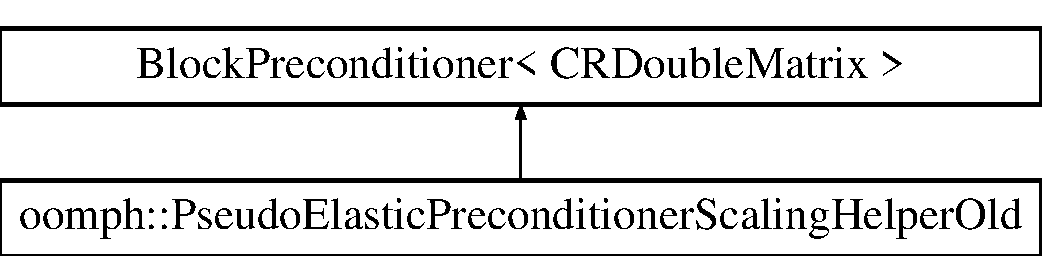
\includegraphics[height=2.000000cm]{classoomph_1_1PseudoElasticPreconditionerScalingHelperOld}
\end{center}
\end{figure}
\subsection*{Public Member Functions}
\begin{DoxyCompactItemize}
\item 
\hyperlink{classoomph_1_1PseudoElasticPreconditionerScalingHelperOld_a90a89541c9067f06446c2a0e9e3c5398}{Pseudo\+Elastic\+Preconditioner\+Scaling\+Helper\+Old} (Block\+Preconditioner$<$ C\+R\+Double\+Matrix $>$ $\ast$master\+\_\+prec\+\_\+pt, C\+R\+Double\+Matrix $\ast$matrix\+\_\+pt, Vector$<$ unsigned $>$ \&dof\+\_\+list, const Mesh $\ast$const solid\+\_\+mesh\+\_\+pt, const Oomph\+Communicator $\ast$comm\+\_\+pt)
\item 
\hyperlink{classoomph_1_1PseudoElasticPreconditionerScalingHelperOld_a330a6acc2a56bf439f0b3d603d392cf8}{$\sim$\+Pseudo\+Elastic\+Preconditioner\+Scaling\+Helper\+Old} ()
\begin{DoxyCompactList}\small\item\em Destructor. \end{DoxyCompactList}\item 
\hyperlink{classoomph_1_1PseudoElasticPreconditionerScalingHelperOld_acfd02d4f3aa04aa04485f2cc8678de5f}{Pseudo\+Elastic\+Preconditioner\+Scaling\+Helper\+Old} (const \hyperlink{classoomph_1_1PseudoElasticPreconditionerScalingHelperOld}{Pseudo\+Elastic\+Preconditioner\+Scaling\+Helper\+Old} \&)
\begin{DoxyCompactList}\small\item\em Broken copy constructor. \end{DoxyCompactList}\item 
double \hyperlink{classoomph_1_1PseudoElasticPreconditionerScalingHelperOld_a4774c6db30bd4f7d054e438add48f7eb}{s\+\_\+inf\+\_\+norm} ()
\begin{DoxyCompactList}\small\item\em Broken assignment operator. \end{DoxyCompactList}\item 
void \hyperlink{classoomph_1_1PseudoElasticPreconditionerScalingHelperOld_a42dca15c6f3678880f3b84ccb91513c7}{setup} ()
\item 
void \hyperlink{classoomph_1_1PseudoElasticPreconditionerScalingHelperOld_a185bc08ce33f220d9ef61745b46e0633}{preconditioner\+\_\+solve} (const Double\+Vector \&r, Double\+Vector \&z)
\end{DoxyCompactItemize}


\subsection{Detailed Description}
A helper class for \hyperlink{classoomph_1_1PseudoElasticPreconditioner}{Pseudo\+Elastic\+Preconditioner}. Note that this is N\+OT actually a functioning preconditioner. We simply derive from this class to get access to the blocks. 

Definition at line 735 of file pseudo\+\_\+elastic\+\_\+preconditioner.\+h.



\subsection{Constructor \& Destructor Documentation}
\mbox{\Hypertarget{classoomph_1_1PseudoElasticPreconditionerScalingHelperOld_a90a89541c9067f06446c2a0e9e3c5398}\label{classoomph_1_1PseudoElasticPreconditionerScalingHelperOld_a90a89541c9067f06446c2a0e9e3c5398}} 
\index{oomph\+::\+Pseudo\+Elastic\+Preconditioner\+Scaling\+Helper\+Old@{oomph\+::\+Pseudo\+Elastic\+Preconditioner\+Scaling\+Helper\+Old}!Pseudo\+Elastic\+Preconditioner\+Scaling\+Helper\+Old@{Pseudo\+Elastic\+Preconditioner\+Scaling\+Helper\+Old}}
\index{Pseudo\+Elastic\+Preconditioner\+Scaling\+Helper\+Old@{Pseudo\+Elastic\+Preconditioner\+Scaling\+Helper\+Old}!oomph\+::\+Pseudo\+Elastic\+Preconditioner\+Scaling\+Helper\+Old@{oomph\+::\+Pseudo\+Elastic\+Preconditioner\+Scaling\+Helper\+Old}}
\subsubsection{\texorpdfstring{Pseudo\+Elastic\+Preconditioner\+Scaling\+Helper\+Old()}{PseudoElasticPreconditionerScalingHelperOld()}\hspace{0.1cm}{\footnotesize\ttfamily [1/2]}}
{\footnotesize\ttfamily oomph\+::\+Pseudo\+Elastic\+Preconditioner\+Scaling\+Helper\+Old\+::\+Pseudo\+Elastic\+Preconditioner\+Scaling\+Helper\+Old (\begin{DoxyParamCaption}\item[{Block\+Preconditioner$<$ C\+R\+Double\+Matrix $>$ $\ast$}]{master\+\_\+prec\+\_\+pt,  }\item[{C\+R\+Double\+Matrix $\ast$}]{matrix\+\_\+pt,  }\item[{Vector$<$ unsigned $>$ \&}]{dof\+\_\+list,  }\item[{const Mesh $\ast$const}]{solid\+\_\+mesh\+\_\+pt,  }\item[{const Oomph\+Communicator $\ast$}]{comm\+\_\+pt }\end{DoxyParamCaption})\hspace{0.3cm}{\ttfamily [inline]}}

The constructor. N\+O\+TE\+:
\begin{DoxyEnumerate}
\item master\+\_\+prec\+\_\+pt should point to the \hyperlink{classoomph_1_1PseudoElasticPreconditioner}{Pseudo\+Elastic\+Preconditioner}.
\item matrix\+\_\+pt should point to the jacobian.
\item The vector dof\+\_\+list should contain the full list of D\+O\+FS associated with the solid subsidiary system.
\item \char`\"{}solid\+\_\+mesh\+\_\+pt\char`\"{} should be a pointer to the solid mesh used in the master preconditioner. 
\end{DoxyEnumerate}

Definition at line 751 of file pseudo\+\_\+elastic\+\_\+preconditioner.\+h.

\mbox{\Hypertarget{classoomph_1_1PseudoElasticPreconditionerScalingHelperOld_a330a6acc2a56bf439f0b3d603d392cf8}\label{classoomph_1_1PseudoElasticPreconditionerScalingHelperOld_a330a6acc2a56bf439f0b3d603d392cf8}} 
\index{oomph\+::\+Pseudo\+Elastic\+Preconditioner\+Scaling\+Helper\+Old@{oomph\+::\+Pseudo\+Elastic\+Preconditioner\+Scaling\+Helper\+Old}!````~Pseudo\+Elastic\+Preconditioner\+Scaling\+Helper\+Old@{$\sim$\+Pseudo\+Elastic\+Preconditioner\+Scaling\+Helper\+Old}}
\index{````~Pseudo\+Elastic\+Preconditioner\+Scaling\+Helper\+Old@{$\sim$\+Pseudo\+Elastic\+Preconditioner\+Scaling\+Helper\+Old}!oomph\+::\+Pseudo\+Elastic\+Preconditioner\+Scaling\+Helper\+Old@{oomph\+::\+Pseudo\+Elastic\+Preconditioner\+Scaling\+Helper\+Old}}
\subsubsection{\texorpdfstring{$\sim$\+Pseudo\+Elastic\+Preconditioner\+Scaling\+Helper\+Old()}{~PseudoElasticPreconditionerScalingHelperOld()}}
{\footnotesize\ttfamily oomph\+::\+Pseudo\+Elastic\+Preconditioner\+Scaling\+Helper\+Old\+::$\sim$\+Pseudo\+Elastic\+Preconditioner\+Scaling\+Helper\+Old (\begin{DoxyParamCaption}{ }\end{DoxyParamCaption})\hspace{0.3cm}{\ttfamily [inline]}}



Destructor. 



Definition at line 778 of file pseudo\+\_\+elastic\+\_\+preconditioner.\+h.

\mbox{\Hypertarget{classoomph_1_1PseudoElasticPreconditionerScalingHelperOld_acfd02d4f3aa04aa04485f2cc8678de5f}\label{classoomph_1_1PseudoElasticPreconditionerScalingHelperOld_acfd02d4f3aa04aa04485f2cc8678de5f}} 
\index{oomph\+::\+Pseudo\+Elastic\+Preconditioner\+Scaling\+Helper\+Old@{oomph\+::\+Pseudo\+Elastic\+Preconditioner\+Scaling\+Helper\+Old}!Pseudo\+Elastic\+Preconditioner\+Scaling\+Helper\+Old@{Pseudo\+Elastic\+Preconditioner\+Scaling\+Helper\+Old}}
\index{Pseudo\+Elastic\+Preconditioner\+Scaling\+Helper\+Old@{Pseudo\+Elastic\+Preconditioner\+Scaling\+Helper\+Old}!oomph\+::\+Pseudo\+Elastic\+Preconditioner\+Scaling\+Helper\+Old@{oomph\+::\+Pseudo\+Elastic\+Preconditioner\+Scaling\+Helper\+Old}}
\subsubsection{\texorpdfstring{Pseudo\+Elastic\+Preconditioner\+Scaling\+Helper\+Old()}{PseudoElasticPreconditionerScalingHelperOld()}\hspace{0.1cm}{\footnotesize\ttfamily [2/2]}}
{\footnotesize\ttfamily oomph\+::\+Pseudo\+Elastic\+Preconditioner\+Scaling\+Helper\+Old\+::\+Pseudo\+Elastic\+Preconditioner\+Scaling\+Helper\+Old (\begin{DoxyParamCaption}\item[{const \hyperlink{classoomph_1_1PseudoElasticPreconditionerScalingHelperOld}{Pseudo\+Elastic\+Preconditioner\+Scaling\+Helper\+Old} \&}]{ }\end{DoxyParamCaption})\hspace{0.3cm}{\ttfamily [inline]}}



Broken copy constructor. 



Definition at line 785 of file pseudo\+\_\+elastic\+\_\+preconditioner.\+h.



\subsection{Member Function Documentation}
\mbox{\Hypertarget{classoomph_1_1PseudoElasticPreconditionerScalingHelperOld_a185bc08ce33f220d9ef61745b46e0633}\label{classoomph_1_1PseudoElasticPreconditionerScalingHelperOld_a185bc08ce33f220d9ef61745b46e0633}} 
\index{oomph\+::\+Pseudo\+Elastic\+Preconditioner\+Scaling\+Helper\+Old@{oomph\+::\+Pseudo\+Elastic\+Preconditioner\+Scaling\+Helper\+Old}!preconditioner\+\_\+solve@{preconditioner\+\_\+solve}}
\index{preconditioner\+\_\+solve@{preconditioner\+\_\+solve}!oomph\+::\+Pseudo\+Elastic\+Preconditioner\+Scaling\+Helper\+Old@{oomph\+::\+Pseudo\+Elastic\+Preconditioner\+Scaling\+Helper\+Old}}
\subsubsection{\texorpdfstring{preconditioner\+\_\+solve()}{preconditioner\_solve()}}
{\footnotesize\ttfamily void oomph\+::\+Pseudo\+Elastic\+Preconditioner\+Scaling\+Helper\+Old\+::preconditioner\+\_\+solve (\begin{DoxyParamCaption}\item[{const Double\+Vector \&}]{r,  }\item[{Double\+Vector \&}]{z }\end{DoxyParamCaption})\hspace{0.3cm}{\ttfamily [inline]}}



Definition at line 822 of file pseudo\+\_\+elastic\+\_\+preconditioner.\+h.

\mbox{\Hypertarget{classoomph_1_1PseudoElasticPreconditionerScalingHelperOld_a4774c6db30bd4f7d054e438add48f7eb}\label{classoomph_1_1PseudoElasticPreconditionerScalingHelperOld_a4774c6db30bd4f7d054e438add48f7eb}} 
\index{oomph\+::\+Pseudo\+Elastic\+Preconditioner\+Scaling\+Helper\+Old@{oomph\+::\+Pseudo\+Elastic\+Preconditioner\+Scaling\+Helper\+Old}!s\+\_\+inf\+\_\+norm@{s\+\_\+inf\+\_\+norm}}
\index{s\+\_\+inf\+\_\+norm@{s\+\_\+inf\+\_\+norm}!oomph\+::\+Pseudo\+Elastic\+Preconditioner\+Scaling\+Helper\+Old@{oomph\+::\+Pseudo\+Elastic\+Preconditioner\+Scaling\+Helper\+Old}}
\subsubsection{\texorpdfstring{s\+\_\+inf\+\_\+norm()}{s\_inf\_norm()}}
{\footnotesize\ttfamily double oomph\+::\+Pseudo\+Elastic\+Preconditioner\+Scaling\+Helper\+Old\+::s\+\_\+inf\+\_\+norm (\begin{DoxyParamCaption}{ }\end{DoxyParamCaption})\hspace{0.3cm}{\ttfamily [inline]}}



Broken assignment operator. 

returns the infinite norm of S 

Definition at line 799 of file pseudo\+\_\+elastic\+\_\+preconditioner.\+h.



Referenced by oomph\+::\+Pseudo\+Elastic\+Preconditioner\+Old\+::setup().

\mbox{\Hypertarget{classoomph_1_1PseudoElasticPreconditionerScalingHelperOld_a42dca15c6f3678880f3b84ccb91513c7}\label{classoomph_1_1PseudoElasticPreconditionerScalingHelperOld_a42dca15c6f3678880f3b84ccb91513c7}} 
\index{oomph\+::\+Pseudo\+Elastic\+Preconditioner\+Scaling\+Helper\+Old@{oomph\+::\+Pseudo\+Elastic\+Preconditioner\+Scaling\+Helper\+Old}!setup@{setup}}
\index{setup@{setup}!oomph\+::\+Pseudo\+Elastic\+Preconditioner\+Scaling\+Helper\+Old@{oomph\+::\+Pseudo\+Elastic\+Preconditioner\+Scaling\+Helper\+Old}}
\subsubsection{\texorpdfstring{setup()}{setup()}}
{\footnotesize\ttfamily void oomph\+::\+Pseudo\+Elastic\+Preconditioner\+Scaling\+Helper\+Old\+::setup (\begin{DoxyParamCaption}{ }\end{DoxyParamCaption})\hspace{0.3cm}{\ttfamily [inline]}}



Definition at line 809 of file pseudo\+\_\+elastic\+\_\+preconditioner.\+h.



The documentation for this class was generated from the following file\+:\begin{DoxyCompactItemize}
\item 
\hyperlink{pseudo__elastic__preconditioner_8h}{pseudo\+\_\+elastic\+\_\+preconditioner.\+h}\end{DoxyCompactItemize}

\hypertarget{classoomph_1_1PseudoElasticPreconditionerSubsidiaryBlockPreconditionerOld}{}\section{oomph\+:\+:Pseudo\+Elastic\+Preconditioner\+Subsidiary\+Block\+Preconditioner\+Old Class Reference}
\label{classoomph_1_1PseudoElasticPreconditionerSubsidiaryBlockPreconditionerOld}\index{oomph\+::\+Pseudo\+Elastic\+Preconditioner\+Subsidiary\+Block\+Preconditioner\+Old@{oomph\+::\+Pseudo\+Elastic\+Preconditioner\+Subsidiary\+Block\+Preconditioner\+Old}}


{\ttfamily \#include $<$pseudo\+\_\+elastic\+\_\+preconditioner.\+h$>$}

Inheritance diagram for oomph\+:\+:Pseudo\+Elastic\+Preconditioner\+Subsidiary\+Block\+Preconditioner\+Old\+:\begin{figure}[H]
\begin{center}
\leavevmode
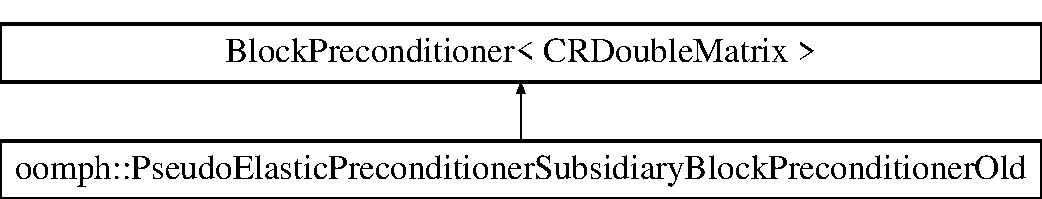
\includegraphics[height=2.000000cm]{classoomph_1_1PseudoElasticPreconditionerSubsidiaryBlockPreconditionerOld}
\end{center}
\end{figure}
\subsection*{Public Types}
\begin{DoxyCompactItemize}
\item 
typedef Preconditioner $\ast$($\ast$ \hyperlink{classoomph_1_1PseudoElasticPreconditionerSubsidiaryBlockPreconditionerOld_a85f57923e70244d5fde0538946eb8c3d}{Subsidiary\+Preconditioner\+Fct\+Pt}) ()
\begin{DoxyCompactList}\small\item\em This preconditioner includes the option to use subsidiary operators other than Super\+L\+U\+Preconditioner for this problem. This is the typedef of a function that should return an instance of a subsidiary preconditioning operator. This preconditioner is responsible for the destruction of the subsidiary preconditioners. \end{DoxyCompactList}\end{DoxyCompactItemize}
\subsection*{Public Member Functions}
\begin{DoxyCompactItemize}
\item 
\hyperlink{classoomph_1_1PseudoElasticPreconditionerSubsidiaryBlockPreconditionerOld_a270a6c5fc522dc82196e89bc6ece086d}{Pseudo\+Elastic\+Preconditioner\+Subsidiary\+Block\+Preconditioner\+Old} ()
\begin{DoxyCompactList}\small\item\em Constructor. (By default this preconditioner is upper triangular). \end{DoxyCompactList}\item 
\hyperlink{classoomph_1_1PseudoElasticPreconditionerSubsidiaryBlockPreconditionerOld_a3d44a67738fba34197376f1a1865bfe1}{$\sim$\+Pseudo\+Elastic\+Preconditioner\+Subsidiary\+Block\+Preconditioner\+Old} ()
\begin{DoxyCompactList}\small\item\em Destructor. \end{DoxyCompactList}\item 
\hyperlink{classoomph_1_1PseudoElasticPreconditionerSubsidiaryBlockPreconditionerOld_a0404c3dde274de59918d3e2e7edd2de2}{Pseudo\+Elastic\+Preconditioner\+Subsidiary\+Block\+Preconditioner\+Old} (const \hyperlink{classoomph_1_1PseudoElasticPreconditionerSubsidiaryBlockPreconditionerOld}{Pseudo\+Elastic\+Preconditioner\+Subsidiary\+Block\+Preconditioner\+Old} \&)
\begin{DoxyCompactList}\small\item\em Broken copy constructor. \end{DoxyCompactList}\item 
void \hyperlink{classoomph_1_1PseudoElasticPreconditionerSubsidiaryBlockPreconditionerOld_a8bb2215735df1a583b4bc1b92bded1e6}{clean\+\_\+up\+\_\+memory} ()
\begin{DoxyCompactList}\small\item\em Broken assignment operator. \end{DoxyCompactList}\item 
void \hyperlink{classoomph_1_1PseudoElasticPreconditionerSubsidiaryBlockPreconditionerOld_a4477e968641690ab5c66c8155aef8a99}{setup} ()
\begin{DoxyCompactList}\small\item\em Setup the preconditioner. \end{DoxyCompactList}\item 
void \hyperlink{classoomph_1_1PseudoElasticPreconditionerSubsidiaryBlockPreconditionerOld_a31f3b927696c11c90f704178cae13e7e}{preconditioner\+\_\+solve} (const Double\+Vector \&res, Double\+Vector \&z)
\begin{DoxyCompactList}\small\item\em Apply preconditioner to r. \end{DoxyCompactList}\item 
void \hyperlink{classoomph_1_1PseudoElasticPreconditionerSubsidiaryBlockPreconditionerOld_a6c238d4e402413fe20061d5735acb40c}{set\+\_\+subsidiary\+\_\+preconditioner\+\_\+function} (\hyperlink{classoomph_1_1PseudoElasticPreconditionerSubsidiaryBlockPreconditionerOld_a85f57923e70244d5fde0538946eb8c3d}{Subsidiary\+Preconditioner\+Fct\+Pt} sub\+\_\+prec\+\_\+fn)
\begin{DoxyCompactList}\small\item\em access function to set the subsidiary preconditioner function. \end{DoxyCompactList}\item 
void \hyperlink{classoomph_1_1PseudoElasticPreconditionerSubsidiaryBlockPreconditionerOld_a1d2c4fa73f0e4839e20ddca2e799da3c}{use\+\_\+block\+\_\+diagonal\+\_\+approximation} ()
\begin{DoxyCompactList}\small\item\em use as a block diagonal preconditioner \end{DoxyCompactList}\item 
void \hyperlink{classoomph_1_1PseudoElasticPreconditionerSubsidiaryBlockPreconditionerOld_a3a6487cc895a4e3a3fe8f978024e116e}{use\+\_\+upper\+\_\+triangular\+\_\+approximation} ()
\begin{DoxyCompactList}\small\item\em Use as an upper triangular preconditioner. \end{DoxyCompactList}\item 
void \hyperlink{classoomph_1_1PseudoElasticPreconditionerSubsidiaryBlockPreconditionerOld_a4ac42f45ed94d02f2fd25b3807653979}{use\+\_\+lower\+\_\+triangular\+\_\+approximation} ()
\begin{DoxyCompactList}\small\item\em Use as a lower triangular preconditioner. \end{DoxyCompactList}\item 
double \& \hyperlink{classoomph_1_1PseudoElasticPreconditionerSubsidiaryBlockPreconditionerOld_ad6cb2301227704660e2f621f9de504cf}{scaling} ()
\begin{DoxyCompactList}\small\item\em Specify the scaling. Default is 1.\+0 Must be set before setup(...). \end{DoxyCompactList}\end{DoxyCompactItemize}
\subsection*{Private Attributes}
\begin{DoxyCompactItemize}
\item 
Vector$<$ \hyperlink{classoomph_1_1PseudoElasticPreconditionerSubsidiaryPreconditionerOld}{Pseudo\+Elastic\+Preconditioner\+Subsidiary\+Preconditioner\+Old} $\ast$ $>$ \hyperlink{classoomph_1_1PseudoElasticPreconditionerSubsidiaryBlockPreconditionerOld_a41bd3e3258d55a595df9af6690df2d2f}{Diagonal\+\_\+block\+\_\+preconditioner\+\_\+pt}
\begin{DoxyCompactList}\small\item\em Vector of Super\+LU preconditioner pointers for storing the preconditioners for each diagonal block. \end{DoxyCompactList}\item 
Dense\+Matrix$<$ Matrix\+Vector\+Product $\ast$ $>$ \hyperlink{classoomph_1_1PseudoElasticPreconditionerSubsidiaryBlockPreconditionerOld_ac736d6b0390de55bb96cc9475a4cabac}{Off\+\_\+diagonal\+\_\+matrix\+\_\+vector\+\_\+products}
\begin{DoxyCompactList}\small\item\em Matrix of matrix vector product operators for the off diagonals. \end{DoxyCompactList}\item 
unsigned \hyperlink{classoomph_1_1PseudoElasticPreconditionerSubsidiaryBlockPreconditionerOld_a6b45cbf207717b9ffe326041f78ea85b}{Method}
\item 
\hyperlink{classoomph_1_1PseudoElasticPreconditionerSubsidiaryBlockPreconditionerOld_a85f57923e70244d5fde0538946eb8c3d}{Subsidiary\+Preconditioner\+Fct\+Pt} \hyperlink{classoomph_1_1PseudoElasticPreconditionerSubsidiaryBlockPreconditionerOld_a376d5fd2ddf9f367854b41478a269ae2}{Subsidiary\+\_\+preconditioner\+\_\+function\+\_\+pt}
\begin{DoxyCompactList}\small\item\em The Subisidary\+Preconditioner\+Fct\+Pt. \end{DoxyCompactList}\item 
double \hyperlink{classoomph_1_1PseudoElasticPreconditionerSubsidiaryBlockPreconditionerOld_a588f4623c606d01c3e3feb3c09023f03}{Scaling}
\begin{DoxyCompactList}\small\item\em The scaling. default 1.\+0. \end{DoxyCompactList}\end{DoxyCompactItemize}


\subsection{Detailed Description}
Subsidiary helper preconditioner for the \hyperlink{classoomph_1_1PseudoElasticPreconditioner}{Pseudo\+Elastic\+Preconditioner}. Required for block preconditioner of the augmented elastic subsidiary problem. N\+O\+TE\+:
\begin{DoxyEnumerate}
\item This is only intended to be used as a subsidiary preconditioner within the \hyperlink{classoomph_1_1PseudoElasticPreconditioner}{Pseudo\+Elastic\+Preconditioner}.
\item If this preconditioner has N D\+OF types then the first N/2 are assumed to be ordinary solid D\+OF types, and the second N/2 are the solid D\+OF types with lagrange multiplier tractions applied.
\item By default this preconditioner uses a superlu preconditioner. 
\end{DoxyEnumerate}

Definition at line 610 of file pseudo\+\_\+elastic\+\_\+preconditioner.\+h.



\subsection{Member Typedef Documentation}
\mbox{\Hypertarget{classoomph_1_1PseudoElasticPreconditionerSubsidiaryBlockPreconditionerOld_a85f57923e70244d5fde0538946eb8c3d}\label{classoomph_1_1PseudoElasticPreconditionerSubsidiaryBlockPreconditionerOld_a85f57923e70244d5fde0538946eb8c3d}} 
\index{oomph\+::\+Pseudo\+Elastic\+Preconditioner\+Subsidiary\+Block\+Preconditioner\+Old@{oomph\+::\+Pseudo\+Elastic\+Preconditioner\+Subsidiary\+Block\+Preconditioner\+Old}!Subsidiary\+Preconditioner\+Fct\+Pt@{Subsidiary\+Preconditioner\+Fct\+Pt}}
\index{Subsidiary\+Preconditioner\+Fct\+Pt@{Subsidiary\+Preconditioner\+Fct\+Pt}!oomph\+::\+Pseudo\+Elastic\+Preconditioner\+Subsidiary\+Block\+Preconditioner\+Old@{oomph\+::\+Pseudo\+Elastic\+Preconditioner\+Subsidiary\+Block\+Preconditioner\+Old}}
\subsubsection{\texorpdfstring{Subsidiary\+Preconditioner\+Fct\+Pt}{SubsidiaryPreconditionerFctPt}}
{\footnotesize\ttfamily typedef Preconditioner$\ast$($\ast$ oomph\+::\+Pseudo\+Elastic\+Preconditioner\+Subsidiary\+Block\+Preconditioner\+Old\+::\+Subsidiary\+Preconditioner\+Fct\+Pt) ()}



This preconditioner includes the option to use subsidiary operators other than Super\+L\+U\+Preconditioner for this problem. This is the typedef of a function that should return an instance of a subsidiary preconditioning operator. This preconditioner is responsible for the destruction of the subsidiary preconditioners. 



Definition at line 620 of file pseudo\+\_\+elastic\+\_\+preconditioner.\+h.



\subsection{Constructor \& Destructor Documentation}
\mbox{\Hypertarget{classoomph_1_1PseudoElasticPreconditionerSubsidiaryBlockPreconditionerOld_a270a6c5fc522dc82196e89bc6ece086d}\label{classoomph_1_1PseudoElasticPreconditionerSubsidiaryBlockPreconditionerOld_a270a6c5fc522dc82196e89bc6ece086d}} 
\index{oomph\+::\+Pseudo\+Elastic\+Preconditioner\+Subsidiary\+Block\+Preconditioner\+Old@{oomph\+::\+Pseudo\+Elastic\+Preconditioner\+Subsidiary\+Block\+Preconditioner\+Old}!Pseudo\+Elastic\+Preconditioner\+Subsidiary\+Block\+Preconditioner\+Old@{Pseudo\+Elastic\+Preconditioner\+Subsidiary\+Block\+Preconditioner\+Old}}
\index{Pseudo\+Elastic\+Preconditioner\+Subsidiary\+Block\+Preconditioner\+Old@{Pseudo\+Elastic\+Preconditioner\+Subsidiary\+Block\+Preconditioner\+Old}!oomph\+::\+Pseudo\+Elastic\+Preconditioner\+Subsidiary\+Block\+Preconditioner\+Old@{oomph\+::\+Pseudo\+Elastic\+Preconditioner\+Subsidiary\+Block\+Preconditioner\+Old}}
\subsubsection{\texorpdfstring{Pseudo\+Elastic\+Preconditioner\+Subsidiary\+Block\+Preconditioner\+Old()}{PseudoElasticPreconditionerSubsidiaryBlockPreconditionerOld()}\hspace{0.1cm}{\footnotesize\ttfamily [1/2]}}
{\footnotesize\ttfamily oomph\+::\+Pseudo\+Elastic\+Preconditioner\+Subsidiary\+Block\+Preconditioner\+Old\+::\+Pseudo\+Elastic\+Preconditioner\+Subsidiary\+Block\+Preconditioner\+Old (\begin{DoxyParamCaption}{ }\end{DoxyParamCaption})\hspace{0.3cm}{\ttfamily [inline]}}



Constructor. (By default this preconditioner is upper triangular). 



Definition at line 623 of file pseudo\+\_\+elastic\+\_\+preconditioner.\+h.

\mbox{\Hypertarget{classoomph_1_1PseudoElasticPreconditionerSubsidiaryBlockPreconditionerOld_a3d44a67738fba34197376f1a1865bfe1}\label{classoomph_1_1PseudoElasticPreconditionerSubsidiaryBlockPreconditionerOld_a3d44a67738fba34197376f1a1865bfe1}} 
\index{oomph\+::\+Pseudo\+Elastic\+Preconditioner\+Subsidiary\+Block\+Preconditioner\+Old@{oomph\+::\+Pseudo\+Elastic\+Preconditioner\+Subsidiary\+Block\+Preconditioner\+Old}!````~Pseudo\+Elastic\+Preconditioner\+Subsidiary\+Block\+Preconditioner\+Old@{$\sim$\+Pseudo\+Elastic\+Preconditioner\+Subsidiary\+Block\+Preconditioner\+Old}}
\index{````~Pseudo\+Elastic\+Preconditioner\+Subsidiary\+Block\+Preconditioner\+Old@{$\sim$\+Pseudo\+Elastic\+Preconditioner\+Subsidiary\+Block\+Preconditioner\+Old}!oomph\+::\+Pseudo\+Elastic\+Preconditioner\+Subsidiary\+Block\+Preconditioner\+Old@{oomph\+::\+Pseudo\+Elastic\+Preconditioner\+Subsidiary\+Block\+Preconditioner\+Old}}
\subsubsection{\texorpdfstring{$\sim$\+Pseudo\+Elastic\+Preconditioner\+Subsidiary\+Block\+Preconditioner\+Old()}{~PseudoElasticPreconditionerSubsidiaryBlockPreconditionerOld()}}
{\footnotesize\ttfamily oomph\+::\+Pseudo\+Elastic\+Preconditioner\+Subsidiary\+Block\+Preconditioner\+Old\+::$\sim$\+Pseudo\+Elastic\+Preconditioner\+Subsidiary\+Block\+Preconditioner\+Old (\begin{DoxyParamCaption}{ }\end{DoxyParamCaption})\hspace{0.3cm}{\ttfamily [inline]}}



Destructor. 



Definition at line 637 of file pseudo\+\_\+elastic\+\_\+preconditioner.\+h.

\mbox{\Hypertarget{classoomph_1_1PseudoElasticPreconditionerSubsidiaryBlockPreconditionerOld_a0404c3dde274de59918d3e2e7edd2de2}\label{classoomph_1_1PseudoElasticPreconditionerSubsidiaryBlockPreconditionerOld_a0404c3dde274de59918d3e2e7edd2de2}} 
\index{oomph\+::\+Pseudo\+Elastic\+Preconditioner\+Subsidiary\+Block\+Preconditioner\+Old@{oomph\+::\+Pseudo\+Elastic\+Preconditioner\+Subsidiary\+Block\+Preconditioner\+Old}!Pseudo\+Elastic\+Preconditioner\+Subsidiary\+Block\+Preconditioner\+Old@{Pseudo\+Elastic\+Preconditioner\+Subsidiary\+Block\+Preconditioner\+Old}}
\index{Pseudo\+Elastic\+Preconditioner\+Subsidiary\+Block\+Preconditioner\+Old@{Pseudo\+Elastic\+Preconditioner\+Subsidiary\+Block\+Preconditioner\+Old}!oomph\+::\+Pseudo\+Elastic\+Preconditioner\+Subsidiary\+Block\+Preconditioner\+Old@{oomph\+::\+Pseudo\+Elastic\+Preconditioner\+Subsidiary\+Block\+Preconditioner\+Old}}
\subsubsection{\texorpdfstring{Pseudo\+Elastic\+Preconditioner\+Subsidiary\+Block\+Preconditioner\+Old()}{PseudoElasticPreconditionerSubsidiaryBlockPreconditionerOld()}\hspace{0.1cm}{\footnotesize\ttfamily [2/2]}}
{\footnotesize\ttfamily oomph\+::\+Pseudo\+Elastic\+Preconditioner\+Subsidiary\+Block\+Preconditioner\+Old\+::\+Pseudo\+Elastic\+Preconditioner\+Subsidiary\+Block\+Preconditioner\+Old (\begin{DoxyParamCaption}\item[{const \hyperlink{classoomph_1_1PseudoElasticPreconditionerSubsidiaryBlockPreconditionerOld}{Pseudo\+Elastic\+Preconditioner\+Subsidiary\+Block\+Preconditioner\+Old} \&}]{ }\end{DoxyParamCaption})\hspace{0.3cm}{\ttfamily [inline]}}



Broken copy constructor. 



Definition at line 644 of file pseudo\+\_\+elastic\+\_\+preconditioner.\+h.



\subsection{Member Function Documentation}
\mbox{\Hypertarget{classoomph_1_1PseudoElasticPreconditionerSubsidiaryBlockPreconditionerOld_a8bb2215735df1a583b4bc1b92bded1e6}\label{classoomph_1_1PseudoElasticPreconditionerSubsidiaryBlockPreconditionerOld_a8bb2215735df1a583b4bc1b92bded1e6}} 
\index{oomph\+::\+Pseudo\+Elastic\+Preconditioner\+Subsidiary\+Block\+Preconditioner\+Old@{oomph\+::\+Pseudo\+Elastic\+Preconditioner\+Subsidiary\+Block\+Preconditioner\+Old}!clean\+\_\+up\+\_\+memory@{clean\+\_\+up\+\_\+memory}}
\index{clean\+\_\+up\+\_\+memory@{clean\+\_\+up\+\_\+memory}!oomph\+::\+Pseudo\+Elastic\+Preconditioner\+Subsidiary\+Block\+Preconditioner\+Old@{oomph\+::\+Pseudo\+Elastic\+Preconditioner\+Subsidiary\+Block\+Preconditioner\+Old}}
\subsubsection{\texorpdfstring{clean\+\_\+up\+\_\+memory()}{clean\_up\_memory()}}
{\footnotesize\ttfamily void oomph\+::\+Pseudo\+Elastic\+Preconditioner\+Subsidiary\+Block\+Preconditioner\+Old\+::clean\+\_\+up\+\_\+memory (\begin{DoxyParamCaption}{ }\end{DoxyParamCaption})}



Broken assignment operator. 

clean up the memory 

Definition at line 945 of file pseudo\+\_\+elastic\+\_\+preconditioner.\+cc.



References setup().



Referenced by oomph\+::\+Pseudo\+Elastic\+Preconditioner\+Subsidiary\+Preconditioner\+Old\+::preconditioner\+\_\+solve().

\mbox{\Hypertarget{classoomph_1_1PseudoElasticPreconditionerSubsidiaryBlockPreconditionerOld_a31f3b927696c11c90f704178cae13e7e}\label{classoomph_1_1PseudoElasticPreconditionerSubsidiaryBlockPreconditionerOld_a31f3b927696c11c90f704178cae13e7e}} 
\index{oomph\+::\+Pseudo\+Elastic\+Preconditioner\+Subsidiary\+Block\+Preconditioner\+Old@{oomph\+::\+Pseudo\+Elastic\+Preconditioner\+Subsidiary\+Block\+Preconditioner\+Old}!preconditioner\+\_\+solve@{preconditioner\+\_\+solve}}
\index{preconditioner\+\_\+solve@{preconditioner\+\_\+solve}!oomph\+::\+Pseudo\+Elastic\+Preconditioner\+Subsidiary\+Block\+Preconditioner\+Old@{oomph\+::\+Pseudo\+Elastic\+Preconditioner\+Subsidiary\+Block\+Preconditioner\+Old}}
\subsubsection{\texorpdfstring{preconditioner\+\_\+solve()}{preconditioner\_solve()}}
{\footnotesize\ttfamily void oomph\+::\+Pseudo\+Elastic\+Preconditioner\+Subsidiary\+Block\+Preconditioner\+Old\+::preconditioner\+\_\+solve (\begin{DoxyParamCaption}\item[{const Double\+Vector \&}]{res,  }\item[{Double\+Vector \&}]{z }\end{DoxyParamCaption})}



Apply preconditioner to r. 



Definition at line 1077 of file pseudo\+\_\+elastic\+\_\+preconditioner.\+cc.



Referenced by setup().

\mbox{\Hypertarget{classoomph_1_1PseudoElasticPreconditionerSubsidiaryBlockPreconditionerOld_ad6cb2301227704660e2f621f9de504cf}\label{classoomph_1_1PseudoElasticPreconditionerSubsidiaryBlockPreconditionerOld_ad6cb2301227704660e2f621f9de504cf}} 
\index{oomph\+::\+Pseudo\+Elastic\+Preconditioner\+Subsidiary\+Block\+Preconditioner\+Old@{oomph\+::\+Pseudo\+Elastic\+Preconditioner\+Subsidiary\+Block\+Preconditioner\+Old}!scaling@{scaling}}
\index{scaling@{scaling}!oomph\+::\+Pseudo\+Elastic\+Preconditioner\+Subsidiary\+Block\+Preconditioner\+Old@{oomph\+::\+Pseudo\+Elastic\+Preconditioner\+Subsidiary\+Block\+Preconditioner\+Old}}
\subsubsection{\texorpdfstring{scaling()}{scaling()}}
{\footnotesize\ttfamily double\& oomph\+::\+Pseudo\+Elastic\+Preconditioner\+Subsidiary\+Block\+Preconditioner\+Old\+::scaling (\begin{DoxyParamCaption}{ }\end{DoxyParamCaption})\hspace{0.3cm}{\ttfamily [inline]}}



Specify the scaling. Default is 1.\+0 Must be set before setup(...). 



Definition at line 694 of file pseudo\+\_\+elastic\+\_\+preconditioner.\+h.



Referenced by oomph\+::\+Pseudo\+Elastic\+Preconditioner\+Old\+::setup().

\mbox{\Hypertarget{classoomph_1_1PseudoElasticPreconditionerSubsidiaryBlockPreconditionerOld_a6c238d4e402413fe20061d5735acb40c}\label{classoomph_1_1PseudoElasticPreconditionerSubsidiaryBlockPreconditionerOld_a6c238d4e402413fe20061d5735acb40c}} 
\index{oomph\+::\+Pseudo\+Elastic\+Preconditioner\+Subsidiary\+Block\+Preconditioner\+Old@{oomph\+::\+Pseudo\+Elastic\+Preconditioner\+Subsidiary\+Block\+Preconditioner\+Old}!set\+\_\+subsidiary\+\_\+preconditioner\+\_\+function@{set\+\_\+subsidiary\+\_\+preconditioner\+\_\+function}}
\index{set\+\_\+subsidiary\+\_\+preconditioner\+\_\+function@{set\+\_\+subsidiary\+\_\+preconditioner\+\_\+function}!oomph\+::\+Pseudo\+Elastic\+Preconditioner\+Subsidiary\+Block\+Preconditioner\+Old@{oomph\+::\+Pseudo\+Elastic\+Preconditioner\+Subsidiary\+Block\+Preconditioner\+Old}}
\subsubsection{\texorpdfstring{set\+\_\+subsidiary\+\_\+preconditioner\+\_\+function()}{set\_subsidiary\_preconditioner\_function()}}
{\footnotesize\ttfamily void oomph\+::\+Pseudo\+Elastic\+Preconditioner\+Subsidiary\+Block\+Preconditioner\+Old\+::set\+\_\+subsidiary\+\_\+preconditioner\+\_\+function (\begin{DoxyParamCaption}\item[{\hyperlink{classoomph_1_1PseudoElasticPreconditionerSubsidiaryBlockPreconditionerOld_a85f57923e70244d5fde0538946eb8c3d}{Subsidiary\+Preconditioner\+Fct\+Pt}}]{sub\+\_\+prec\+\_\+fn }\end{DoxyParamCaption})\hspace{0.3cm}{\ttfamily [inline]}}



access function to set the subsidiary preconditioner function. 



Definition at line 669 of file pseudo\+\_\+elastic\+\_\+preconditioner.\+h.

\mbox{\Hypertarget{classoomph_1_1PseudoElasticPreconditionerSubsidiaryBlockPreconditionerOld_a4477e968641690ab5c66c8155aef8a99}\label{classoomph_1_1PseudoElasticPreconditionerSubsidiaryBlockPreconditionerOld_a4477e968641690ab5c66c8155aef8a99}} 
\index{oomph\+::\+Pseudo\+Elastic\+Preconditioner\+Subsidiary\+Block\+Preconditioner\+Old@{oomph\+::\+Pseudo\+Elastic\+Preconditioner\+Subsidiary\+Block\+Preconditioner\+Old}!setup@{setup}}
\index{setup@{setup}!oomph\+::\+Pseudo\+Elastic\+Preconditioner\+Subsidiary\+Block\+Preconditioner\+Old@{oomph\+::\+Pseudo\+Elastic\+Preconditioner\+Subsidiary\+Block\+Preconditioner\+Old}}
\subsubsection{\texorpdfstring{setup()}{setup()}}
{\footnotesize\ttfamily void oomph\+::\+Pseudo\+Elastic\+Preconditioner\+Subsidiary\+Block\+Preconditioner\+Old\+::setup (\begin{DoxyParamCaption}{ }\end{DoxyParamCaption})}



Setup the preconditioner. 



Definition at line 981 of file pseudo\+\_\+elastic\+\_\+preconditioner.\+cc.



References preconditioner\+\_\+solve().



Referenced by clean\+\_\+up\+\_\+memory().

\mbox{\Hypertarget{classoomph_1_1PseudoElasticPreconditionerSubsidiaryBlockPreconditionerOld_a1d2c4fa73f0e4839e20ddca2e799da3c}\label{classoomph_1_1PseudoElasticPreconditionerSubsidiaryBlockPreconditionerOld_a1d2c4fa73f0e4839e20ddca2e799da3c}} 
\index{oomph\+::\+Pseudo\+Elastic\+Preconditioner\+Subsidiary\+Block\+Preconditioner\+Old@{oomph\+::\+Pseudo\+Elastic\+Preconditioner\+Subsidiary\+Block\+Preconditioner\+Old}!use\+\_\+block\+\_\+diagonal\+\_\+approximation@{use\+\_\+block\+\_\+diagonal\+\_\+approximation}}
\index{use\+\_\+block\+\_\+diagonal\+\_\+approximation@{use\+\_\+block\+\_\+diagonal\+\_\+approximation}!oomph\+::\+Pseudo\+Elastic\+Preconditioner\+Subsidiary\+Block\+Preconditioner\+Old@{oomph\+::\+Pseudo\+Elastic\+Preconditioner\+Subsidiary\+Block\+Preconditioner\+Old}}
\subsubsection{\texorpdfstring{use\+\_\+block\+\_\+diagonal\+\_\+approximation()}{use\_block\_diagonal\_approximation()}}
{\footnotesize\ttfamily void oomph\+::\+Pseudo\+Elastic\+Preconditioner\+Subsidiary\+Block\+Preconditioner\+Old\+::use\+\_\+block\+\_\+diagonal\+\_\+approximation (\begin{DoxyParamCaption}{ }\end{DoxyParamCaption})\hspace{0.3cm}{\ttfamily [inline]}}



use as a block diagonal preconditioner 



Definition at line 675 of file pseudo\+\_\+elastic\+\_\+preconditioner.\+h.



Referenced by oomph\+::\+Pseudo\+Elastic\+Preconditioner\+Old\+::setup().

\mbox{\Hypertarget{classoomph_1_1PseudoElasticPreconditionerSubsidiaryBlockPreconditionerOld_a4ac42f45ed94d02f2fd25b3807653979}\label{classoomph_1_1PseudoElasticPreconditionerSubsidiaryBlockPreconditionerOld_a4ac42f45ed94d02f2fd25b3807653979}} 
\index{oomph\+::\+Pseudo\+Elastic\+Preconditioner\+Subsidiary\+Block\+Preconditioner\+Old@{oomph\+::\+Pseudo\+Elastic\+Preconditioner\+Subsidiary\+Block\+Preconditioner\+Old}!use\+\_\+lower\+\_\+triangular\+\_\+approximation@{use\+\_\+lower\+\_\+triangular\+\_\+approximation}}
\index{use\+\_\+lower\+\_\+triangular\+\_\+approximation@{use\+\_\+lower\+\_\+triangular\+\_\+approximation}!oomph\+::\+Pseudo\+Elastic\+Preconditioner\+Subsidiary\+Block\+Preconditioner\+Old@{oomph\+::\+Pseudo\+Elastic\+Preconditioner\+Subsidiary\+Block\+Preconditioner\+Old}}
\subsubsection{\texorpdfstring{use\+\_\+lower\+\_\+triangular\+\_\+approximation()}{use\_lower\_triangular\_approximation()}}
{\footnotesize\ttfamily void oomph\+::\+Pseudo\+Elastic\+Preconditioner\+Subsidiary\+Block\+Preconditioner\+Old\+::use\+\_\+lower\+\_\+triangular\+\_\+approximation (\begin{DoxyParamCaption}{ }\end{DoxyParamCaption})\hspace{0.3cm}{\ttfamily [inline]}}



Use as a lower triangular preconditioner. 



Definition at line 687 of file pseudo\+\_\+elastic\+\_\+preconditioner.\+h.



Referenced by oomph\+::\+Pseudo\+Elastic\+Preconditioner\+Old\+::setup().

\mbox{\Hypertarget{classoomph_1_1PseudoElasticPreconditionerSubsidiaryBlockPreconditionerOld_a3a6487cc895a4e3a3fe8f978024e116e}\label{classoomph_1_1PseudoElasticPreconditionerSubsidiaryBlockPreconditionerOld_a3a6487cc895a4e3a3fe8f978024e116e}} 
\index{oomph\+::\+Pseudo\+Elastic\+Preconditioner\+Subsidiary\+Block\+Preconditioner\+Old@{oomph\+::\+Pseudo\+Elastic\+Preconditioner\+Subsidiary\+Block\+Preconditioner\+Old}!use\+\_\+upper\+\_\+triangular\+\_\+approximation@{use\+\_\+upper\+\_\+triangular\+\_\+approximation}}
\index{use\+\_\+upper\+\_\+triangular\+\_\+approximation@{use\+\_\+upper\+\_\+triangular\+\_\+approximation}!oomph\+::\+Pseudo\+Elastic\+Preconditioner\+Subsidiary\+Block\+Preconditioner\+Old@{oomph\+::\+Pseudo\+Elastic\+Preconditioner\+Subsidiary\+Block\+Preconditioner\+Old}}
\subsubsection{\texorpdfstring{use\+\_\+upper\+\_\+triangular\+\_\+approximation()}{use\_upper\_triangular\_approximation()}}
{\footnotesize\ttfamily void oomph\+::\+Pseudo\+Elastic\+Preconditioner\+Subsidiary\+Block\+Preconditioner\+Old\+::use\+\_\+upper\+\_\+triangular\+\_\+approximation (\begin{DoxyParamCaption}{ }\end{DoxyParamCaption})\hspace{0.3cm}{\ttfamily [inline]}}



Use as an upper triangular preconditioner. 



Definition at line 681 of file pseudo\+\_\+elastic\+\_\+preconditioner.\+h.



Referenced by oomph\+::\+Pseudo\+Elastic\+Preconditioner\+Old\+::setup().



\subsection{Member Data Documentation}
\mbox{\Hypertarget{classoomph_1_1PseudoElasticPreconditionerSubsidiaryBlockPreconditionerOld_a41bd3e3258d55a595df9af6690df2d2f}\label{classoomph_1_1PseudoElasticPreconditionerSubsidiaryBlockPreconditionerOld_a41bd3e3258d55a595df9af6690df2d2f}} 
\index{oomph\+::\+Pseudo\+Elastic\+Preconditioner\+Subsidiary\+Block\+Preconditioner\+Old@{oomph\+::\+Pseudo\+Elastic\+Preconditioner\+Subsidiary\+Block\+Preconditioner\+Old}!Diagonal\+\_\+block\+\_\+preconditioner\+\_\+pt@{Diagonal\+\_\+block\+\_\+preconditioner\+\_\+pt}}
\index{Diagonal\+\_\+block\+\_\+preconditioner\+\_\+pt@{Diagonal\+\_\+block\+\_\+preconditioner\+\_\+pt}!oomph\+::\+Pseudo\+Elastic\+Preconditioner\+Subsidiary\+Block\+Preconditioner\+Old@{oomph\+::\+Pseudo\+Elastic\+Preconditioner\+Subsidiary\+Block\+Preconditioner\+Old}}
\subsubsection{\texorpdfstring{Diagonal\+\_\+block\+\_\+preconditioner\+\_\+pt}{Diagonal\_block\_preconditioner\_pt}}
{\footnotesize\ttfamily Vector$<$\hyperlink{classoomph_1_1PseudoElasticPreconditionerSubsidiaryPreconditionerOld}{Pseudo\+Elastic\+Preconditioner\+Subsidiary\+Preconditioner\+Old}$\ast$$>$ oomph\+::\+Pseudo\+Elastic\+Preconditioner\+Subsidiary\+Block\+Preconditioner\+Old\+::\+Diagonal\+\_\+block\+\_\+preconditioner\+\_\+pt\hspace{0.3cm}{\ttfamily [private]}}



Vector of Super\+LU preconditioner pointers for storing the preconditioners for each diagonal block. 



Definition at line 704 of file pseudo\+\_\+elastic\+\_\+preconditioner.\+h.

\mbox{\Hypertarget{classoomph_1_1PseudoElasticPreconditionerSubsidiaryBlockPreconditionerOld_a6b45cbf207717b9ffe326041f78ea85b}\label{classoomph_1_1PseudoElasticPreconditionerSubsidiaryBlockPreconditionerOld_a6b45cbf207717b9ffe326041f78ea85b}} 
\index{oomph\+::\+Pseudo\+Elastic\+Preconditioner\+Subsidiary\+Block\+Preconditioner\+Old@{oomph\+::\+Pseudo\+Elastic\+Preconditioner\+Subsidiary\+Block\+Preconditioner\+Old}!Method@{Method}}
\index{Method@{Method}!oomph\+::\+Pseudo\+Elastic\+Preconditioner\+Subsidiary\+Block\+Preconditioner\+Old@{oomph\+::\+Pseudo\+Elastic\+Preconditioner\+Subsidiary\+Block\+Preconditioner\+Old}}
\subsubsection{\texorpdfstring{Method}{Method}}
{\footnotesize\ttfamily unsigned oomph\+::\+Pseudo\+Elastic\+Preconditioner\+Subsidiary\+Block\+Preconditioner\+Old\+::\+Method\hspace{0.3cm}{\ttfamily [private]}}

the preconditioning method. 0 -\/ block diagonal 1 -\/ upper triangular 2 -\/ lower triangular 

Definition at line 713 of file pseudo\+\_\+elastic\+\_\+preconditioner.\+h.

\mbox{\Hypertarget{classoomph_1_1PseudoElasticPreconditionerSubsidiaryBlockPreconditionerOld_ac736d6b0390de55bb96cc9475a4cabac}\label{classoomph_1_1PseudoElasticPreconditionerSubsidiaryBlockPreconditionerOld_ac736d6b0390de55bb96cc9475a4cabac}} 
\index{oomph\+::\+Pseudo\+Elastic\+Preconditioner\+Subsidiary\+Block\+Preconditioner\+Old@{oomph\+::\+Pseudo\+Elastic\+Preconditioner\+Subsidiary\+Block\+Preconditioner\+Old}!Off\+\_\+diagonal\+\_\+matrix\+\_\+vector\+\_\+products@{Off\+\_\+diagonal\+\_\+matrix\+\_\+vector\+\_\+products}}
\index{Off\+\_\+diagonal\+\_\+matrix\+\_\+vector\+\_\+products@{Off\+\_\+diagonal\+\_\+matrix\+\_\+vector\+\_\+products}!oomph\+::\+Pseudo\+Elastic\+Preconditioner\+Subsidiary\+Block\+Preconditioner\+Old@{oomph\+::\+Pseudo\+Elastic\+Preconditioner\+Subsidiary\+Block\+Preconditioner\+Old}}
\subsubsection{\texorpdfstring{Off\+\_\+diagonal\+\_\+matrix\+\_\+vector\+\_\+products}{Off\_diagonal\_matrix\_vector\_products}}
{\footnotesize\ttfamily Dense\+Matrix$<$Matrix\+Vector\+Product$\ast$$>$ oomph\+::\+Pseudo\+Elastic\+Preconditioner\+Subsidiary\+Block\+Preconditioner\+Old\+::\+Off\+\_\+diagonal\+\_\+matrix\+\_\+vector\+\_\+products\hspace{0.3cm}{\ttfamily [private]}}



Matrix of matrix vector product operators for the off diagonals. 



Definition at line 707 of file pseudo\+\_\+elastic\+\_\+preconditioner.\+h.

\mbox{\Hypertarget{classoomph_1_1PseudoElasticPreconditionerSubsidiaryBlockPreconditionerOld_a588f4623c606d01c3e3feb3c09023f03}\label{classoomph_1_1PseudoElasticPreconditionerSubsidiaryBlockPreconditionerOld_a588f4623c606d01c3e3feb3c09023f03}} 
\index{oomph\+::\+Pseudo\+Elastic\+Preconditioner\+Subsidiary\+Block\+Preconditioner\+Old@{oomph\+::\+Pseudo\+Elastic\+Preconditioner\+Subsidiary\+Block\+Preconditioner\+Old}!Scaling@{Scaling}}
\index{Scaling@{Scaling}!oomph\+::\+Pseudo\+Elastic\+Preconditioner\+Subsidiary\+Block\+Preconditioner\+Old@{oomph\+::\+Pseudo\+Elastic\+Preconditioner\+Subsidiary\+Block\+Preconditioner\+Old}}
\subsubsection{\texorpdfstring{Scaling}{Scaling}}
{\footnotesize\ttfamily double oomph\+::\+Pseudo\+Elastic\+Preconditioner\+Subsidiary\+Block\+Preconditioner\+Old\+::\+Scaling\hspace{0.3cm}{\ttfamily [private]}}



The scaling. default 1.\+0. 



Definition at line 719 of file pseudo\+\_\+elastic\+\_\+preconditioner.\+h.

\mbox{\Hypertarget{classoomph_1_1PseudoElasticPreconditionerSubsidiaryBlockPreconditionerOld_a376d5fd2ddf9f367854b41478a269ae2}\label{classoomph_1_1PseudoElasticPreconditionerSubsidiaryBlockPreconditionerOld_a376d5fd2ddf9f367854b41478a269ae2}} 
\index{oomph\+::\+Pseudo\+Elastic\+Preconditioner\+Subsidiary\+Block\+Preconditioner\+Old@{oomph\+::\+Pseudo\+Elastic\+Preconditioner\+Subsidiary\+Block\+Preconditioner\+Old}!Subsidiary\+\_\+preconditioner\+\_\+function\+\_\+pt@{Subsidiary\+\_\+preconditioner\+\_\+function\+\_\+pt}}
\index{Subsidiary\+\_\+preconditioner\+\_\+function\+\_\+pt@{Subsidiary\+\_\+preconditioner\+\_\+function\+\_\+pt}!oomph\+::\+Pseudo\+Elastic\+Preconditioner\+Subsidiary\+Block\+Preconditioner\+Old@{oomph\+::\+Pseudo\+Elastic\+Preconditioner\+Subsidiary\+Block\+Preconditioner\+Old}}
\subsubsection{\texorpdfstring{Subsidiary\+\_\+preconditioner\+\_\+function\+\_\+pt}{Subsidiary\_preconditioner\_function\_pt}}
{\footnotesize\ttfamily \hyperlink{classoomph_1_1PseudoElasticPreconditionerSubsidiaryBlockPreconditionerOld_a85f57923e70244d5fde0538946eb8c3d}{Subsidiary\+Preconditioner\+Fct\+Pt} oomph\+::\+Pseudo\+Elastic\+Preconditioner\+Subsidiary\+Block\+Preconditioner\+Old\+::\+Subsidiary\+\_\+preconditioner\+\_\+function\+\_\+pt\hspace{0.3cm}{\ttfamily [private]}}



The Subisidary\+Preconditioner\+Fct\+Pt. 



Definition at line 716 of file pseudo\+\_\+elastic\+\_\+preconditioner.\+h.



The documentation for this class was generated from the following files\+:\begin{DoxyCompactItemize}
\item 
\hyperlink{pseudo__elastic__preconditioner_8h}{pseudo\+\_\+elastic\+\_\+preconditioner.\+h}\item 
\hyperlink{pseudo__elastic__preconditioner_8cc}{pseudo\+\_\+elastic\+\_\+preconditioner.\+cc}\end{DoxyCompactItemize}

\hypertarget{classoomph_1_1PseudoElasticPreconditionerSubsidiaryPreconditionerOld}{}\section{oomph\+:\+:Pseudo\+Elastic\+Preconditioner\+Subsidiary\+Preconditioner\+Old Class Reference}
\label{classoomph_1_1PseudoElasticPreconditionerSubsidiaryPreconditionerOld}\index{oomph\+::\+Pseudo\+Elastic\+Preconditioner\+Subsidiary\+Preconditioner\+Old@{oomph\+::\+Pseudo\+Elastic\+Preconditioner\+Subsidiary\+Preconditioner\+Old}}


{\ttfamily \#include $<$pseudo\+\_\+elastic\+\_\+preconditioner.\+h$>$}

Inheritance diagram for oomph\+:\+:Pseudo\+Elastic\+Preconditioner\+Subsidiary\+Preconditioner\+Old\+:\begin{figure}[H]
\begin{center}
\leavevmode
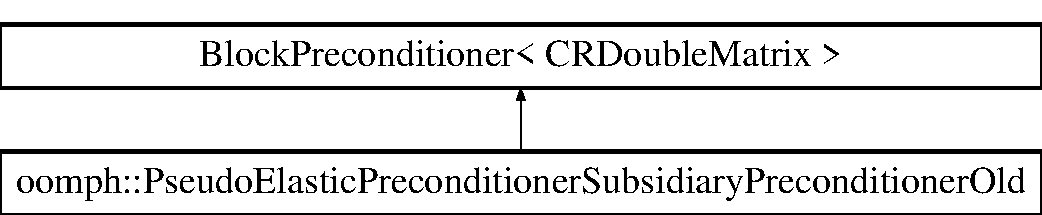
\includegraphics[height=4.000000cm]{classoomph_1_1PseudoElasticPreconditionerSubsidiaryPreconditionerOld}
\end{center}
\end{figure}
\subsection*{Public Types}
\begin{DoxyCompactItemize}
\item 
typedef \hyperlink{classoomph_1_1Preconditioner}{Preconditioner} $\ast$($\ast$ \hyperlink{classoomph_1_1PseudoElasticPreconditionerSubsidiaryPreconditionerOld_a2ee5b7ddad26a4eb6662e2b701ab0a52}{Subsidiary\+Preconditioner\+Fct\+Pt}) ()
\begin{DoxyCompactList}\small\item\em typedef for a function that allows other preconditioners to be emplyed to solve the subsidiary linear systems. The function should return a pointer to the requred subsidiary preconditioner generated using new. This preconditioner is responsible for the destruction of the subsidiary preconditioners. \end{DoxyCompactList}\end{DoxyCompactItemize}
\subsection*{Public Member Functions}
\begin{DoxyCompactItemize}
\item 
\hyperlink{classoomph_1_1PseudoElasticPreconditionerSubsidiaryPreconditionerOld_a674640dd0de0b3a40857c01e8b868928}{Pseudo\+Elastic\+Preconditioner\+Subsidiary\+Preconditioner\+Old} ()
\begin{DoxyCompactList}\small\item\em Constructor. \end{DoxyCompactList}\item 
\hyperlink{classoomph_1_1PseudoElasticPreconditionerSubsidiaryPreconditionerOld_a231e24badc0c56a577af50891100ecb7}{$\sim$\+Pseudo\+Elastic\+Preconditioner\+Subsidiary\+Preconditioner\+Old} ()
\begin{DoxyCompactList}\small\item\em Destructor. \end{DoxyCompactList}\item 
\hyperlink{classoomph_1_1PseudoElasticPreconditionerSubsidiaryPreconditionerOld_a58a3b8721c6c171175b520315782498b}{Pseudo\+Elastic\+Preconditioner\+Subsidiary\+Preconditioner\+Old} (const \hyperlink{classoomph_1_1PseudoElasticPreconditionerSubsidiaryPreconditionerOld}{Pseudo\+Elastic\+Preconditioner\+Subsidiary\+Preconditioner\+Old} \&)
\begin{DoxyCompactList}\small\item\em Broken copy constructor. \end{DoxyCompactList}\item 
void \hyperlink{classoomph_1_1PseudoElasticPreconditionerSubsidiaryPreconditionerOld_a532201f17edc43b3b475fff2d2744b8b}{setup} ()
\begin{DoxyCompactList}\small\item\em Broken assignment operator. \end{DoxyCompactList}\item 
void \hyperlink{classoomph_1_1PseudoElasticPreconditionerSubsidiaryPreconditionerOld_a01d70c9e3454b52c86f4439d29fd4b22}{preconditioner\+\_\+solve} (const \hyperlink{classoomph_1_1DoubleVector}{Double\+Vector} \&r, \hyperlink{classoomph_1_1DoubleVector}{Double\+Vector} \&z)
\begin{DoxyCompactList}\small\item\em Apply the preconditioner. \end{DoxyCompactList}\item 
double \& \hyperlink{classoomph_1_1PseudoElasticPreconditionerSubsidiaryPreconditionerOld_a38a9cf93e354ea1fbb76f8d8fa1df0ab}{scaling} ()
\begin{DoxyCompactList}\small\item\em Specify the scaling. Default is 1.\+0 Must be called before setup(...). \end{DoxyCompactList}\item 
void \hyperlink{classoomph_1_1PseudoElasticPreconditionerSubsidiaryPreconditionerOld_a6fd50251d78370846929956b3eabf310}{set\+\_\+subsidiary\+\_\+preconditioner\+\_\+function} (\hyperlink{classoomph_1_1PseudoElasticPreconditionerSubsidiaryPreconditionerOld_a2ee5b7ddad26a4eb6662e2b701ab0a52}{Subsidiary\+Preconditioner\+Fct\+Pt} sub\+\_\+prec\+\_\+fn)
\begin{DoxyCompactList}\small\item\em access function to set the subsidiary preconditioner function. \end{DoxyCompactList}\end{DoxyCompactItemize}
\subsection*{Private Member Functions}
\begin{DoxyCompactItemize}
\item 
void \hyperlink{classoomph_1_1PseudoElasticPreconditionerSubsidiaryPreconditionerOld_a45086bd75b2d82f65deae8cac23c4c47}{clean\+\_\+up\+\_\+memory} ()
\begin{DoxyCompactList}\small\item\em clears the memory \end{DoxyCompactList}\end{DoxyCompactItemize}
\subsection*{Private Attributes}
\begin{DoxyCompactItemize}
\item 
double \hyperlink{classoomph_1_1PseudoElasticPreconditionerSubsidiaryPreconditionerOld_a9815c3c63cc82fcfb7bcd914459e5445}{Scaling}
\item 
\hyperlink{classoomph_1_1Preconditioner}{Preconditioner} $\ast$ \hyperlink{classoomph_1_1PseudoElasticPreconditionerSubsidiaryPreconditionerOld_a48413dd5490629563b76bb34b1e2e256}{Preconditioner\+\_\+pt}
\begin{DoxyCompactList}\small\item\em the preconditioner pt \end{DoxyCompactList}\item 
\hyperlink{classoomph_1_1PseudoElasticPreconditionerSubsidiaryPreconditionerOld_a2ee5b7ddad26a4eb6662e2b701ab0a52}{Subsidiary\+Preconditioner\+Fct\+Pt} \hyperlink{classoomph_1_1PseudoElasticPreconditionerSubsidiaryPreconditionerOld_a15876ef914c08070cc025f3b6696e4e1}{Subsidiary\+\_\+preconditioner\+\_\+function\+\_\+pt}
\begin{DoxyCompactList}\small\item\em the Subisidary\+Preconditioner\+Fct\+Pt \end{DoxyCompactList}\end{DoxyCompactItemize}
\subsection*{Additional Inherited Members}


\subsection{Detailed Description}
Subsidiary helper preconditioner for the \hyperlink{classoomph_1_1PseudoElasticPreconditioner}{Pseudo\+Elastic\+Preconditioner}. Required to construct the augmented elastic system prior to preconditioning. N\+O\+TE\+:
\begin{DoxyEnumerate}
\item This is only intended to be used as a subsidiary preconditioner within the \hyperlink{classoomph_1_1PseudoElasticPreconditioner}{Pseudo\+Elastic\+Preconditioner}.
\item If this preconditioner has N D\+OF types then the first N/2 are assumed to be ordinary solid D\+OF types, and the second N/2 are the solid D\+OF types with lagrange multiplier tractions applied.
\item By default this preconditioner uses a superlu preconditioner. 
\end{DoxyEnumerate}

Definition at line 509 of file pseudo\+\_\+elastic\+\_\+preconditioner.\+h.



\subsection{Member Typedef Documentation}
\mbox{\Hypertarget{classoomph_1_1PseudoElasticPreconditionerSubsidiaryPreconditionerOld_a2ee5b7ddad26a4eb6662e2b701ab0a52}\label{classoomph_1_1PseudoElasticPreconditionerSubsidiaryPreconditionerOld_a2ee5b7ddad26a4eb6662e2b701ab0a52}} 
\index{oomph\+::\+Pseudo\+Elastic\+Preconditioner\+Subsidiary\+Preconditioner\+Old@{oomph\+::\+Pseudo\+Elastic\+Preconditioner\+Subsidiary\+Preconditioner\+Old}!Subsidiary\+Preconditioner\+Fct\+Pt@{Subsidiary\+Preconditioner\+Fct\+Pt}}
\index{Subsidiary\+Preconditioner\+Fct\+Pt@{Subsidiary\+Preconditioner\+Fct\+Pt}!oomph\+::\+Pseudo\+Elastic\+Preconditioner\+Subsidiary\+Preconditioner\+Old@{oomph\+::\+Pseudo\+Elastic\+Preconditioner\+Subsidiary\+Preconditioner\+Old}}
\subsubsection{\texorpdfstring{Subsidiary\+Preconditioner\+Fct\+Pt}{SubsidiaryPreconditionerFctPt}}
{\footnotesize\ttfamily typedef \hyperlink{classoomph_1_1Preconditioner}{Preconditioner}$\ast$($\ast$ oomph\+::\+Pseudo\+Elastic\+Preconditioner\+Subsidiary\+Preconditioner\+Old\+::\+Subsidiary\+Preconditioner\+Fct\+Pt) ()}



typedef for a function that allows other preconditioners to be emplyed to solve the subsidiary linear systems. The function should return a pointer to the requred subsidiary preconditioner generated using new. This preconditioner is responsible for the destruction of the subsidiary preconditioners. 



Definition at line 520 of file pseudo\+\_\+elastic\+\_\+preconditioner.\+h.



\subsection{Constructor \& Destructor Documentation}
\mbox{\Hypertarget{classoomph_1_1PseudoElasticPreconditionerSubsidiaryPreconditionerOld_a674640dd0de0b3a40857c01e8b868928}\label{classoomph_1_1PseudoElasticPreconditionerSubsidiaryPreconditionerOld_a674640dd0de0b3a40857c01e8b868928}} 
\index{oomph\+::\+Pseudo\+Elastic\+Preconditioner\+Subsidiary\+Preconditioner\+Old@{oomph\+::\+Pseudo\+Elastic\+Preconditioner\+Subsidiary\+Preconditioner\+Old}!Pseudo\+Elastic\+Preconditioner\+Subsidiary\+Preconditioner\+Old@{Pseudo\+Elastic\+Preconditioner\+Subsidiary\+Preconditioner\+Old}}
\index{Pseudo\+Elastic\+Preconditioner\+Subsidiary\+Preconditioner\+Old@{Pseudo\+Elastic\+Preconditioner\+Subsidiary\+Preconditioner\+Old}!oomph\+::\+Pseudo\+Elastic\+Preconditioner\+Subsidiary\+Preconditioner\+Old@{oomph\+::\+Pseudo\+Elastic\+Preconditioner\+Subsidiary\+Preconditioner\+Old}}
\subsubsection{\texorpdfstring{Pseudo\+Elastic\+Preconditioner\+Subsidiary\+Preconditioner\+Old()}{PseudoElasticPreconditionerSubsidiaryPreconditionerOld()}\hspace{0.1cm}{\footnotesize\ttfamily [1/2]}}
{\footnotesize\ttfamily oomph\+::\+Pseudo\+Elastic\+Preconditioner\+Subsidiary\+Preconditioner\+Old\+::\+Pseudo\+Elastic\+Preconditioner\+Subsidiary\+Preconditioner\+Old (\begin{DoxyParamCaption}{ }\end{DoxyParamCaption})\hspace{0.3cm}{\ttfamily [inline]}}



Constructor. 



Definition at line 523 of file pseudo\+\_\+elastic\+\_\+preconditioner.\+h.

\mbox{\Hypertarget{classoomph_1_1PseudoElasticPreconditionerSubsidiaryPreconditionerOld_a231e24badc0c56a577af50891100ecb7}\label{classoomph_1_1PseudoElasticPreconditionerSubsidiaryPreconditionerOld_a231e24badc0c56a577af50891100ecb7}} 
\index{oomph\+::\+Pseudo\+Elastic\+Preconditioner\+Subsidiary\+Preconditioner\+Old@{oomph\+::\+Pseudo\+Elastic\+Preconditioner\+Subsidiary\+Preconditioner\+Old}!````~Pseudo\+Elastic\+Preconditioner\+Subsidiary\+Preconditioner\+Old@{$\sim$\+Pseudo\+Elastic\+Preconditioner\+Subsidiary\+Preconditioner\+Old}}
\index{````~Pseudo\+Elastic\+Preconditioner\+Subsidiary\+Preconditioner\+Old@{$\sim$\+Pseudo\+Elastic\+Preconditioner\+Subsidiary\+Preconditioner\+Old}!oomph\+::\+Pseudo\+Elastic\+Preconditioner\+Subsidiary\+Preconditioner\+Old@{oomph\+::\+Pseudo\+Elastic\+Preconditioner\+Subsidiary\+Preconditioner\+Old}}
\subsubsection{\texorpdfstring{$\sim$\+Pseudo\+Elastic\+Preconditioner\+Subsidiary\+Preconditioner\+Old()}{~PseudoElasticPreconditionerSubsidiaryPreconditionerOld()}}
{\footnotesize\ttfamily oomph\+::\+Pseudo\+Elastic\+Preconditioner\+Subsidiary\+Preconditioner\+Old\+::$\sim$\+Pseudo\+Elastic\+Preconditioner\+Subsidiary\+Preconditioner\+Old (\begin{DoxyParamCaption}{ }\end{DoxyParamCaption})\hspace{0.3cm}{\ttfamily [inline]}}



Destructor. 



Definition at line 531 of file pseudo\+\_\+elastic\+\_\+preconditioner.\+h.

\mbox{\Hypertarget{classoomph_1_1PseudoElasticPreconditionerSubsidiaryPreconditionerOld_a58a3b8721c6c171175b520315782498b}\label{classoomph_1_1PseudoElasticPreconditionerSubsidiaryPreconditionerOld_a58a3b8721c6c171175b520315782498b}} 
\index{oomph\+::\+Pseudo\+Elastic\+Preconditioner\+Subsidiary\+Preconditioner\+Old@{oomph\+::\+Pseudo\+Elastic\+Preconditioner\+Subsidiary\+Preconditioner\+Old}!Pseudo\+Elastic\+Preconditioner\+Subsidiary\+Preconditioner\+Old@{Pseudo\+Elastic\+Preconditioner\+Subsidiary\+Preconditioner\+Old}}
\index{Pseudo\+Elastic\+Preconditioner\+Subsidiary\+Preconditioner\+Old@{Pseudo\+Elastic\+Preconditioner\+Subsidiary\+Preconditioner\+Old}!oomph\+::\+Pseudo\+Elastic\+Preconditioner\+Subsidiary\+Preconditioner\+Old@{oomph\+::\+Pseudo\+Elastic\+Preconditioner\+Subsidiary\+Preconditioner\+Old}}
\subsubsection{\texorpdfstring{Pseudo\+Elastic\+Preconditioner\+Subsidiary\+Preconditioner\+Old()}{PseudoElasticPreconditionerSubsidiaryPreconditionerOld()}\hspace{0.1cm}{\footnotesize\ttfamily [2/2]}}
{\footnotesize\ttfamily oomph\+::\+Pseudo\+Elastic\+Preconditioner\+Subsidiary\+Preconditioner\+Old\+::\+Pseudo\+Elastic\+Preconditioner\+Subsidiary\+Preconditioner\+Old (\begin{DoxyParamCaption}\item[{const \hyperlink{classoomph_1_1PseudoElasticPreconditionerSubsidiaryPreconditionerOld}{Pseudo\+Elastic\+Preconditioner\+Subsidiary\+Preconditioner\+Old} \&}]{ }\end{DoxyParamCaption})\hspace{0.3cm}{\ttfamily [inline]}}



Broken copy constructor. 



Definition at line 538 of file pseudo\+\_\+elastic\+\_\+preconditioner.\+h.



References oomph\+::\+Broken\+Copy\+::broken\+\_\+copy(), and oomph\+::\+Terminate\+Helper\+::setup().



\subsection{Member Function Documentation}
\mbox{\Hypertarget{classoomph_1_1PseudoElasticPreconditionerSubsidiaryPreconditionerOld_a45086bd75b2d82f65deae8cac23c4c47}\label{classoomph_1_1PseudoElasticPreconditionerSubsidiaryPreconditionerOld_a45086bd75b2d82f65deae8cac23c4c47}} 
\index{oomph\+::\+Pseudo\+Elastic\+Preconditioner\+Subsidiary\+Preconditioner\+Old@{oomph\+::\+Pseudo\+Elastic\+Preconditioner\+Subsidiary\+Preconditioner\+Old}!clean\+\_\+up\+\_\+memory@{clean\+\_\+up\+\_\+memory}}
\index{clean\+\_\+up\+\_\+memory@{clean\+\_\+up\+\_\+memory}!oomph\+::\+Pseudo\+Elastic\+Preconditioner\+Subsidiary\+Preconditioner\+Old@{oomph\+::\+Pseudo\+Elastic\+Preconditioner\+Subsidiary\+Preconditioner\+Old}}
\subsubsection{\texorpdfstring{clean\+\_\+up\+\_\+memory()}{clean\_up\_memory()}}
{\footnotesize\ttfamily void oomph\+::\+Pseudo\+Elastic\+Preconditioner\+Subsidiary\+Preconditioner\+Old\+::clean\+\_\+up\+\_\+memory (\begin{DoxyParamCaption}{ }\end{DoxyParamCaption})\hspace{0.3cm}{\ttfamily [inline]}, {\ttfamily [private]}, {\ttfamily [virtual]}}



clears the memory 



Reimplemented from \hyperlink{classoomph_1_1Preconditioner_a46c31c416829bedcd9db238431262027}{oomph\+::\+Preconditioner}.



Definition at line 574 of file pseudo\+\_\+elastic\+\_\+preconditioner.\+h.

\mbox{\Hypertarget{classoomph_1_1PseudoElasticPreconditionerSubsidiaryPreconditionerOld_a01d70c9e3454b52c86f4439d29fd4b22}\label{classoomph_1_1PseudoElasticPreconditionerSubsidiaryPreconditionerOld_a01d70c9e3454b52c86f4439d29fd4b22}} 
\index{oomph\+::\+Pseudo\+Elastic\+Preconditioner\+Subsidiary\+Preconditioner\+Old@{oomph\+::\+Pseudo\+Elastic\+Preconditioner\+Subsidiary\+Preconditioner\+Old}!preconditioner\+\_\+solve@{preconditioner\+\_\+solve}}
\index{preconditioner\+\_\+solve@{preconditioner\+\_\+solve}!oomph\+::\+Pseudo\+Elastic\+Preconditioner\+Subsidiary\+Preconditioner\+Old@{oomph\+::\+Pseudo\+Elastic\+Preconditioner\+Subsidiary\+Preconditioner\+Old}}
\subsubsection{\texorpdfstring{preconditioner\+\_\+solve()}{preconditioner\_solve()}}
{\footnotesize\ttfamily void oomph\+::\+Pseudo\+Elastic\+Preconditioner\+Subsidiary\+Preconditioner\+Old\+::preconditioner\+\_\+solve (\begin{DoxyParamCaption}\item[{const \hyperlink{classoomph_1_1DoubleVector}{Double\+Vector} \&}]{r,  }\item[{\hyperlink{classoomph_1_1DoubleVector}{Double\+Vector} \&}]{z }\end{DoxyParamCaption})\hspace{0.3cm}{\ttfamily [virtual]}}



Apply the preconditioner. 



Implements \hyperlink{classoomph_1_1Preconditioner_ace1199369e4465cd2b9a34884bb64ec8}{oomph\+::\+Preconditioner}.



Definition at line 924 of file pseudo\+\_\+elastic\+\_\+preconditioner.\+cc.



References oomph\+::\+Pseudo\+Elastic\+Preconditioner\+Subsidiary\+Block\+Preconditioner\+Old\+::clean\+\_\+up\+\_\+memory().



Referenced by setup().

\mbox{\Hypertarget{classoomph_1_1PseudoElasticPreconditionerSubsidiaryPreconditionerOld_a38a9cf93e354ea1fbb76f8d8fa1df0ab}\label{classoomph_1_1PseudoElasticPreconditionerSubsidiaryPreconditionerOld_a38a9cf93e354ea1fbb76f8d8fa1df0ab}} 
\index{oomph\+::\+Pseudo\+Elastic\+Preconditioner\+Subsidiary\+Preconditioner\+Old@{oomph\+::\+Pseudo\+Elastic\+Preconditioner\+Subsidiary\+Preconditioner\+Old}!scaling@{scaling}}
\index{scaling@{scaling}!oomph\+::\+Pseudo\+Elastic\+Preconditioner\+Subsidiary\+Preconditioner\+Old@{oomph\+::\+Pseudo\+Elastic\+Preconditioner\+Subsidiary\+Preconditioner\+Old}}
\subsubsection{\texorpdfstring{scaling()}{scaling()}}
{\footnotesize\ttfamily double\& oomph\+::\+Pseudo\+Elastic\+Preconditioner\+Subsidiary\+Preconditioner\+Old\+::scaling (\begin{DoxyParamCaption}{ }\end{DoxyParamCaption})\hspace{0.3cm}{\ttfamily [inline]}}



Specify the scaling. Default is 1.\+0 Must be called before setup(...). 



Definition at line 559 of file pseudo\+\_\+elastic\+\_\+preconditioner.\+h.



Referenced by oomph\+::\+Pseudo\+Elastic\+Preconditioner\+Old\+::setup().

\mbox{\Hypertarget{classoomph_1_1PseudoElasticPreconditionerSubsidiaryPreconditionerOld_a6fd50251d78370846929956b3eabf310}\label{classoomph_1_1PseudoElasticPreconditionerSubsidiaryPreconditionerOld_a6fd50251d78370846929956b3eabf310}} 
\index{oomph\+::\+Pseudo\+Elastic\+Preconditioner\+Subsidiary\+Preconditioner\+Old@{oomph\+::\+Pseudo\+Elastic\+Preconditioner\+Subsidiary\+Preconditioner\+Old}!set\+\_\+subsidiary\+\_\+preconditioner\+\_\+function@{set\+\_\+subsidiary\+\_\+preconditioner\+\_\+function}}
\index{set\+\_\+subsidiary\+\_\+preconditioner\+\_\+function@{set\+\_\+subsidiary\+\_\+preconditioner\+\_\+function}!oomph\+::\+Pseudo\+Elastic\+Preconditioner\+Subsidiary\+Preconditioner\+Old@{oomph\+::\+Pseudo\+Elastic\+Preconditioner\+Subsidiary\+Preconditioner\+Old}}
\subsubsection{\texorpdfstring{set\+\_\+subsidiary\+\_\+preconditioner\+\_\+function()}{set\_subsidiary\_preconditioner\_function()}}
{\footnotesize\ttfamily void oomph\+::\+Pseudo\+Elastic\+Preconditioner\+Subsidiary\+Preconditioner\+Old\+::set\+\_\+subsidiary\+\_\+preconditioner\+\_\+function (\begin{DoxyParamCaption}\item[{\hyperlink{classoomph_1_1PseudoElasticPreconditionerSubsidiaryPreconditionerOld_a2ee5b7ddad26a4eb6662e2b701ab0a52}{Subsidiary\+Preconditioner\+Fct\+Pt}}]{sub\+\_\+prec\+\_\+fn }\end{DoxyParamCaption})\hspace{0.3cm}{\ttfamily [inline]}}



access function to set the subsidiary preconditioner function. 



Definition at line 566 of file pseudo\+\_\+elastic\+\_\+preconditioner.\+h.

\mbox{\Hypertarget{classoomph_1_1PseudoElasticPreconditionerSubsidiaryPreconditionerOld_a532201f17edc43b3b475fff2d2744b8b}\label{classoomph_1_1PseudoElasticPreconditionerSubsidiaryPreconditionerOld_a532201f17edc43b3b475fff2d2744b8b}} 
\index{oomph\+::\+Pseudo\+Elastic\+Preconditioner\+Subsidiary\+Preconditioner\+Old@{oomph\+::\+Pseudo\+Elastic\+Preconditioner\+Subsidiary\+Preconditioner\+Old}!setup@{setup}}
\index{setup@{setup}!oomph\+::\+Pseudo\+Elastic\+Preconditioner\+Subsidiary\+Preconditioner\+Old@{oomph\+::\+Pseudo\+Elastic\+Preconditioner\+Subsidiary\+Preconditioner\+Old}}
\subsubsection{\texorpdfstring{setup()}{setup()}}
{\footnotesize\ttfamily void oomph\+::\+Pseudo\+Elastic\+Preconditioner\+Subsidiary\+Preconditioner\+Old\+::setup (\begin{DoxyParamCaption}{ }\end{DoxyParamCaption})\hspace{0.3cm}{\ttfamily [virtual]}}



Broken assignment operator. 

Setup the preconditioner. 

Implements \hyperlink{classoomph_1_1Preconditioner_af4886f4efe510e5c9b0eb19422943588}{oomph\+::\+Preconditioner}.



Definition at line 838 of file pseudo\+\_\+elastic\+\_\+preconditioner.\+cc.



References oomph\+::\+C\+R\+Double\+Matrix\+::column\+\_\+index(), oomph\+::\+Distributable\+Linear\+Algebra\+Object\+::first\+\_\+row(), i, oomph\+::\+Distributable\+Linear\+Algebra\+Object\+::nrow\+\_\+local(), preconditioner\+\_\+solve(), oomph\+::\+C\+R\+Double\+Matrix\+::row\+\_\+start(), oomph\+::\+Super\+L\+U\+Preconditioner\+::setup(), and oomph\+::\+C\+R\+Double\+Matrix\+::value().



Referenced by oomph\+::\+Pseudo\+Elastic\+Preconditioner\+Old\+::clean\+\_\+up\+\_\+memory().



\subsection{Member Data Documentation}
\mbox{\Hypertarget{classoomph_1_1PseudoElasticPreconditionerSubsidiaryPreconditionerOld_a48413dd5490629563b76bb34b1e2e256}\label{classoomph_1_1PseudoElasticPreconditionerSubsidiaryPreconditionerOld_a48413dd5490629563b76bb34b1e2e256}} 
\index{oomph\+::\+Pseudo\+Elastic\+Preconditioner\+Subsidiary\+Preconditioner\+Old@{oomph\+::\+Pseudo\+Elastic\+Preconditioner\+Subsidiary\+Preconditioner\+Old}!Preconditioner\+\_\+pt@{Preconditioner\+\_\+pt}}
\index{Preconditioner\+\_\+pt@{Preconditioner\+\_\+pt}!oomph\+::\+Pseudo\+Elastic\+Preconditioner\+Subsidiary\+Preconditioner\+Old@{oomph\+::\+Pseudo\+Elastic\+Preconditioner\+Subsidiary\+Preconditioner\+Old}}
\subsubsection{\texorpdfstring{Preconditioner\+\_\+pt}{Preconditioner\_pt}}
{\footnotesize\ttfamily \hyperlink{classoomph_1_1Preconditioner}{Preconditioner}$\ast$ oomph\+::\+Pseudo\+Elastic\+Preconditioner\+Subsidiary\+Preconditioner\+Old\+::\+Preconditioner\+\_\+pt\hspace{0.3cm}{\ttfamily [private]}}



the preconditioner pt 



Definition at line 584 of file pseudo\+\_\+elastic\+\_\+preconditioner.\+h.

\mbox{\Hypertarget{classoomph_1_1PseudoElasticPreconditionerSubsidiaryPreconditionerOld_a9815c3c63cc82fcfb7bcd914459e5445}\label{classoomph_1_1PseudoElasticPreconditionerSubsidiaryPreconditionerOld_a9815c3c63cc82fcfb7bcd914459e5445}} 
\index{oomph\+::\+Pseudo\+Elastic\+Preconditioner\+Subsidiary\+Preconditioner\+Old@{oomph\+::\+Pseudo\+Elastic\+Preconditioner\+Subsidiary\+Preconditioner\+Old}!Scaling@{Scaling}}
\index{Scaling@{Scaling}!oomph\+::\+Pseudo\+Elastic\+Preconditioner\+Subsidiary\+Preconditioner\+Old@{oomph\+::\+Pseudo\+Elastic\+Preconditioner\+Subsidiary\+Preconditioner\+Old}}
\subsubsection{\texorpdfstring{Scaling}{Scaling}}
{\footnotesize\ttfamily double oomph\+::\+Pseudo\+Elastic\+Preconditioner\+Subsidiary\+Preconditioner\+Old\+::\+Scaling\hspace{0.3cm}{\ttfamily [private]}}



Definition at line 581 of file pseudo\+\_\+elastic\+\_\+preconditioner.\+h.

\mbox{\Hypertarget{classoomph_1_1PseudoElasticPreconditionerSubsidiaryPreconditionerOld_a15876ef914c08070cc025f3b6696e4e1}\label{classoomph_1_1PseudoElasticPreconditionerSubsidiaryPreconditionerOld_a15876ef914c08070cc025f3b6696e4e1}} 
\index{oomph\+::\+Pseudo\+Elastic\+Preconditioner\+Subsidiary\+Preconditioner\+Old@{oomph\+::\+Pseudo\+Elastic\+Preconditioner\+Subsidiary\+Preconditioner\+Old}!Subsidiary\+\_\+preconditioner\+\_\+function\+\_\+pt@{Subsidiary\+\_\+preconditioner\+\_\+function\+\_\+pt}}
\index{Subsidiary\+\_\+preconditioner\+\_\+function\+\_\+pt@{Subsidiary\+\_\+preconditioner\+\_\+function\+\_\+pt}!oomph\+::\+Pseudo\+Elastic\+Preconditioner\+Subsidiary\+Preconditioner\+Old@{oomph\+::\+Pseudo\+Elastic\+Preconditioner\+Subsidiary\+Preconditioner\+Old}}
\subsubsection{\texorpdfstring{Subsidiary\+\_\+preconditioner\+\_\+function\+\_\+pt}{Subsidiary\_preconditioner\_function\_pt}}
{\footnotesize\ttfamily \hyperlink{classoomph_1_1PseudoElasticPreconditionerSubsidiaryPreconditionerOld_a2ee5b7ddad26a4eb6662e2b701ab0a52}{Subsidiary\+Preconditioner\+Fct\+Pt} oomph\+::\+Pseudo\+Elastic\+Preconditioner\+Subsidiary\+Preconditioner\+Old\+::\+Subsidiary\+\_\+preconditioner\+\_\+function\+\_\+pt\hspace{0.3cm}{\ttfamily [private]}}



the Subisidary\+Preconditioner\+Fct\+Pt 



Definition at line 587 of file pseudo\+\_\+elastic\+\_\+preconditioner.\+h.



The documentation for this class was generated from the following files\+:\begin{DoxyCompactItemize}
\item 
\hyperlink{pseudo__elastic__preconditioner_8h}{pseudo\+\_\+elastic\+\_\+preconditioner.\+h}\item 
\hyperlink{pseudo__elastic__preconditioner_8cc}{pseudo\+\_\+elastic\+\_\+preconditioner.\+cc}\end{DoxyCompactItemize}

\hypertarget{classoomph_1_1RefineableAdvectionDiffusionBoussinesqElement}{}\section{oomph\+:\+:Refineable\+Advection\+Diffusion\+Boussinesq\+Element$<$ A\+D\+\_\+\+E\+L\+E\+M\+E\+NT, N\+S\+T\+\_\+\+E\+L\+E\+M\+E\+NT $>$ Class Template Reference}
\label{classoomph_1_1RefineableAdvectionDiffusionBoussinesqElement}\index{oomph\+::\+Refineable\+Advection\+Diffusion\+Boussinesq\+Element$<$ A\+D\+\_\+\+E\+L\+E\+M\+E\+N\+T, N\+S\+T\+\_\+\+E\+L\+E\+M\+E\+N\+T $>$@{oomph\+::\+Refineable\+Advection\+Diffusion\+Boussinesq\+Element$<$ A\+D\+\_\+\+E\+L\+E\+M\+E\+N\+T, N\+S\+T\+\_\+\+E\+L\+E\+M\+E\+N\+T $>$}}


{\ttfamily \#include $<$multi\+\_\+domain\+\_\+boussinesq\+\_\+elements.\+h$>$}

Inheritance diagram for oomph\+:\+:Refineable\+Advection\+Diffusion\+Boussinesq\+Element$<$ A\+D\+\_\+\+E\+L\+E\+M\+E\+NT, N\+S\+T\+\_\+\+E\+L\+E\+M\+E\+NT $>$\+:\begin{figure}[H]
\begin{center}
\leavevmode
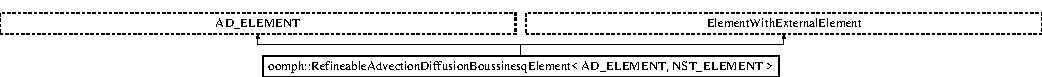
\includegraphics[height=1.033210cm]{classoomph_1_1RefineableAdvectionDiffusionBoussinesqElement}
\end{center}
\end{figure}
\subsection*{Public Member Functions}
\begin{DoxyCompactItemize}
\item 
\hyperlink{classoomph_1_1RefineableAdvectionDiffusionBoussinesqElement_a26f91df92dc910d525ec920b9d674046}{Refineable\+Advection\+Diffusion\+Boussinesq\+Element} ()
\begin{DoxyCompactList}\small\item\em Constructor\+: call the underlying constructors. \end{DoxyCompactList}\item 
void \hyperlink{classoomph_1_1RefineableAdvectionDiffusionBoussinesqElement_a91bd582775205de08b7c0092acc82a0d}{output} (std\+::ostream \&outfile, const unsigned \&nplot)
\begin{DoxyCompactList}\small\item\em Output function\+: Output x, y, theta at Nplot$^\wedge$\+D\+IM plot points. \end{DoxyCompactList}\item 
void \hyperlink{classoomph_1_1RefineableAdvectionDiffusionBoussinesqElement_ae56c984aaa1aeddf1f458e700ffbe6a1}{output} (std\+::ostream \&outfile)
\begin{DoxyCompactList}\small\item\em Overload the standard output function with the broken default. \end{DoxyCompactList}\item 
void \hyperlink{classoomph_1_1RefineableAdvectionDiffusionBoussinesqElement_ac8fa2a491b9c5bda7bcfdd93d0a00b11}{output} (F\+I\+LE $\ast$file\+\_\+pt)
\begin{DoxyCompactList}\small\item\em C-\/style output function\+: Broken default. \end{DoxyCompactList}\item 
void \hyperlink{classoomph_1_1RefineableAdvectionDiffusionBoussinesqElement_a61bcd2e4a50f8e157ca40572b384dcee}{output} (F\+I\+LE $\ast$file\+\_\+pt, const unsigned \&n\+\_\+plot)
\begin{DoxyCompactList}\small\item\em C-\/style output function\+: Broken default. \end{DoxyCompactList}\item 
void \hyperlink{classoomph_1_1RefineableAdvectionDiffusionBoussinesqElement_a8279f67a0b2150be8f80d51c647f5e9e}{get\+\_\+wind\+\_\+adv\+\_\+diff} (const unsigned \&ipt, const Vector$<$ double $>$ \&s, const Vector$<$ double $>$ \&x, Vector$<$ double $>$ \&wind) const
\begin{DoxyCompactList}\small\item\em Overload the wind function in the advection-\/diffusion equations. This provides the coupling from the Navier--Stokes equations to the advection-\/diffusion equations because the wind is the fluid velocity, obtained from the \char`\"{}external\char`\"{} element. \end{DoxyCompactList}\item 
void \hyperlink{classoomph_1_1RefineableAdvectionDiffusionBoussinesqElement_a89bbdff66fd1fe24f4ae1d681a88d583}{fill\+\_\+in\+\_\+contribution\+\_\+to\+\_\+jacobian} (Vector$<$ double $>$ \&residuals, Dense\+Matrix$<$ double $>$ \&jacobian)
\begin{DoxyCompactList}\small\item\em Compute the element\textquotesingle{}s residual vector and the Jacobian matrix. \end{DoxyCompactList}\item 
void \hyperlink{classoomph_1_1RefineableAdvectionDiffusionBoussinesqElement_abb212175a68a9686ead329ba9fa330f6}{identify\+\_\+all\+\_\+field\+\_\+data\+\_\+for\+\_\+external\+\_\+interaction} (Vector$<$ std\+::set$<$ Finite\+Element $\ast$$>$ $>$ const \&external\+\_\+elements\+\_\+pt, std\+::set$<$ std\+::pair$<$ Data $\ast$, unsigned $>$ $>$ \&paired\+\_\+interaction\+\_\+data)
\begin{DoxyCompactList}\small\item\em Overload the function that must return all field data involved in the interaction with the external (Navier Stokes) element. Only the velocity dofs in the Navier Stokes element affect the interaction with the current element. \end{DoxyCompactList}\item 
void \hyperlink{classoomph_1_1RefineableAdvectionDiffusionBoussinesqElement_a25627bf0853bda6c520a2b1c2c602af4}{fill\+\_\+in\+\_\+contribution\+\_\+to\+\_\+jacobian\+\_\+and\+\_\+mass\+\_\+matrix} (Vector$<$ double $>$ \&residuals, Dense\+Matrix$<$ double $>$ \&jacobian, Dense\+Matrix$<$ double $>$ \&mass\+\_\+matrix)
\begin{DoxyCompactList}\small\item\em Add the element\textquotesingle{}s contribution to its residuals vector, jacobian matrix and mass matrix. \end{DoxyCompactList}\item 
void \hyperlink{classoomph_1_1RefineableAdvectionDiffusionBoussinesqElement_a560911c835c054a25b5e5d8390cc422c}{get\+\_\+dwind\+\_\+adv\+\_\+diff\+\_\+dexternal\+\_\+element\+\_\+data} (const unsigned \&ipt, const unsigned \&i, Vector$<$ double $>$ \&result, Vector$<$ unsigned $>$ \&global\+\_\+eqn\+\_\+number)
\begin{DoxyCompactList}\small\item\em Fill in the derivatives of the wind with respect to the external unknowns. \end{DoxyCompactList}\item 
void \hyperlink{classoomph_1_1RefineableAdvectionDiffusionBoussinesqElement_ac787480832d09daf1bd1f14715dc6820}{fill\+\_\+in\+\_\+off\+\_\+diagonal\+\_\+block\+\_\+analytic} (Vector$<$ double $>$ \&residuals, Dense\+Matrix$<$ double $>$ \&jacobian)
\begin{DoxyCompactList}\small\item\em Compute the contribution of the external degrees of freedom (velocities) on the advection-\/diffusion equations. \end{DoxyCompactList}\item 
void \hyperlink{classoomph_1_1RefineableAdvectionDiffusionBoussinesqElement_a9b48b8a752432bce03a4bc51785d0151}{get\+\_\+dof\+\_\+numbers\+\_\+for\+\_\+unknowns} (std\+::list$<$ std\+::pair$<$ unsigned long, unsigned $>$ $>$ \&dof\+\_\+lookup\+\_\+list) const
\begin{DoxyCompactList}\small\item\em Classify dofs for use in block preconditioner. \end{DoxyCompactList}\item 
unsigned \hyperlink{classoomph_1_1RefineableAdvectionDiffusionBoussinesqElement_adee164161a19b307d37831c98d256d58}{ndof\+\_\+types} () const
\begin{DoxyCompactList}\small\item\em Specify number of dof types for use in block preconditioner. \end{DoxyCompactList}\end{DoxyCompactItemize}


\subsection{Detailed Description}
\subsubsection*{template$<$class A\+D\+\_\+\+E\+L\+E\+M\+E\+NT, class N\+S\+T\+\_\+\+E\+L\+E\+M\+E\+NT$>$\newline
class oomph\+::\+Refineable\+Advection\+Diffusion\+Boussinesq\+Element$<$ A\+D\+\_\+\+E\+L\+E\+M\+E\+N\+T, N\+S\+T\+\_\+\+E\+L\+E\+M\+E\+N\+T $>$}

Build an Advection\+Diffusion\+Element that inherits from Element\+With\+External\+Element so that it can \char`\"{}communicate\char`\"{} with the a Navier\+Stokes\+Element that provides its wind. 

Definition at line 381 of file multi\+\_\+domain\+\_\+boussinesq\+\_\+elements.\+h.



\subsection{Constructor \& Destructor Documentation}
\mbox{\Hypertarget{classoomph_1_1RefineableAdvectionDiffusionBoussinesqElement_a26f91df92dc910d525ec920b9d674046}\label{classoomph_1_1RefineableAdvectionDiffusionBoussinesqElement_a26f91df92dc910d525ec920b9d674046}} 
\index{oomph\+::\+Refineable\+Advection\+Diffusion\+Boussinesq\+Element@{oomph\+::\+Refineable\+Advection\+Diffusion\+Boussinesq\+Element}!Refineable\+Advection\+Diffusion\+Boussinesq\+Element@{Refineable\+Advection\+Diffusion\+Boussinesq\+Element}}
\index{Refineable\+Advection\+Diffusion\+Boussinesq\+Element@{Refineable\+Advection\+Diffusion\+Boussinesq\+Element}!oomph\+::\+Refineable\+Advection\+Diffusion\+Boussinesq\+Element@{oomph\+::\+Refineable\+Advection\+Diffusion\+Boussinesq\+Element}}
\subsubsection{\texorpdfstring{Refineable\+Advection\+Diffusion\+Boussinesq\+Element()}{RefineableAdvectionDiffusionBoussinesqElement()}}
{\footnotesize\ttfamily template$<$class A\+D\+\_\+\+E\+L\+E\+M\+E\+NT , class N\+S\+T\+\_\+\+E\+L\+E\+M\+E\+NT $>$ \\
\hyperlink{classoomph_1_1RefineableAdvectionDiffusionBoussinesqElement}{oomph\+::\+Refineable\+Advection\+Diffusion\+Boussinesq\+Element}$<$ A\+D\+\_\+\+E\+L\+E\+M\+E\+NT, N\+S\+T\+\_\+\+E\+L\+E\+M\+E\+NT $>$\+::\hyperlink{classoomph_1_1RefineableAdvectionDiffusionBoussinesqElement}{Refineable\+Advection\+Diffusion\+Boussinesq\+Element} (\begin{DoxyParamCaption}{ }\end{DoxyParamCaption})\hspace{0.3cm}{\ttfamily [inline]}}



Constructor\+: call the underlying constructors. 



Definition at line 388 of file multi\+\_\+domain\+\_\+boussinesq\+\_\+elements.\+h.



\subsection{Member Function Documentation}
\mbox{\Hypertarget{classoomph_1_1RefineableAdvectionDiffusionBoussinesqElement_a89bbdff66fd1fe24f4ae1d681a88d583}\label{classoomph_1_1RefineableAdvectionDiffusionBoussinesqElement_a89bbdff66fd1fe24f4ae1d681a88d583}} 
\index{oomph\+::\+Refineable\+Advection\+Diffusion\+Boussinesq\+Element@{oomph\+::\+Refineable\+Advection\+Diffusion\+Boussinesq\+Element}!fill\+\_\+in\+\_\+contribution\+\_\+to\+\_\+jacobian@{fill\+\_\+in\+\_\+contribution\+\_\+to\+\_\+jacobian}}
\index{fill\+\_\+in\+\_\+contribution\+\_\+to\+\_\+jacobian@{fill\+\_\+in\+\_\+contribution\+\_\+to\+\_\+jacobian}!oomph\+::\+Refineable\+Advection\+Diffusion\+Boussinesq\+Element@{oomph\+::\+Refineable\+Advection\+Diffusion\+Boussinesq\+Element}}
\subsubsection{\texorpdfstring{fill\+\_\+in\+\_\+contribution\+\_\+to\+\_\+jacobian()}{fill\_in\_contribution\_to\_jacobian()}}
{\footnotesize\ttfamily template$<$class A\+D\+\_\+\+E\+L\+E\+M\+E\+NT , class N\+S\+T\+\_\+\+E\+L\+E\+M\+E\+NT $>$ \\
void \hyperlink{classoomph_1_1RefineableAdvectionDiffusionBoussinesqElement}{oomph\+::\+Refineable\+Advection\+Diffusion\+Boussinesq\+Element}$<$ A\+D\+\_\+\+E\+L\+E\+M\+E\+NT, N\+S\+T\+\_\+\+E\+L\+E\+M\+E\+NT $>$\+::fill\+\_\+in\+\_\+contribution\+\_\+to\+\_\+jacobian (\begin{DoxyParamCaption}\item[{Vector$<$ double $>$ \&}]{residuals,  }\item[{Dense\+Matrix$<$ double $>$ \&}]{jacobian }\end{DoxyParamCaption})\hspace{0.3cm}{\ttfamily [inline]}}



Compute the element\textquotesingle{}s residual vector and the Jacobian matrix. 



Definition at line 472 of file multi\+\_\+domain\+\_\+boussinesq\+\_\+elements.\+h.

\mbox{\Hypertarget{classoomph_1_1RefineableAdvectionDiffusionBoussinesqElement_a25627bf0853bda6c520a2b1c2c602af4}\label{classoomph_1_1RefineableAdvectionDiffusionBoussinesqElement_a25627bf0853bda6c520a2b1c2c602af4}} 
\index{oomph\+::\+Refineable\+Advection\+Diffusion\+Boussinesq\+Element@{oomph\+::\+Refineable\+Advection\+Diffusion\+Boussinesq\+Element}!fill\+\_\+in\+\_\+contribution\+\_\+to\+\_\+jacobian\+\_\+and\+\_\+mass\+\_\+matrix@{fill\+\_\+in\+\_\+contribution\+\_\+to\+\_\+jacobian\+\_\+and\+\_\+mass\+\_\+matrix}}
\index{fill\+\_\+in\+\_\+contribution\+\_\+to\+\_\+jacobian\+\_\+and\+\_\+mass\+\_\+matrix@{fill\+\_\+in\+\_\+contribution\+\_\+to\+\_\+jacobian\+\_\+and\+\_\+mass\+\_\+matrix}!oomph\+::\+Refineable\+Advection\+Diffusion\+Boussinesq\+Element@{oomph\+::\+Refineable\+Advection\+Diffusion\+Boussinesq\+Element}}
\subsubsection{\texorpdfstring{fill\+\_\+in\+\_\+contribution\+\_\+to\+\_\+jacobian\+\_\+and\+\_\+mass\+\_\+matrix()}{fill\_in\_contribution\_to\_jacobian\_and\_mass\_matrix()}}
{\footnotesize\ttfamily template$<$class A\+D\+\_\+\+E\+L\+E\+M\+E\+NT , class N\+S\+T\+\_\+\+E\+L\+E\+M\+E\+NT $>$ \\
void \hyperlink{classoomph_1_1RefineableAdvectionDiffusionBoussinesqElement}{oomph\+::\+Refineable\+Advection\+Diffusion\+Boussinesq\+Element}$<$ A\+D\+\_\+\+E\+L\+E\+M\+E\+NT, N\+S\+T\+\_\+\+E\+L\+E\+M\+E\+NT $>$\+::fill\+\_\+in\+\_\+contribution\+\_\+to\+\_\+jacobian\+\_\+and\+\_\+mass\+\_\+matrix (\begin{DoxyParamCaption}\item[{Vector$<$ double $>$ \&}]{residuals,  }\item[{Dense\+Matrix$<$ double $>$ \&}]{jacobian,  }\item[{Dense\+Matrix$<$ double $>$ \&}]{mass\+\_\+matrix }\end{DoxyParamCaption})\hspace{0.3cm}{\ttfamily [inline]}}



Add the element\textquotesingle{}s contribution to its residuals vector, jacobian matrix and mass matrix. 



Definition at line 503 of file multi\+\_\+domain\+\_\+boussinesq\+\_\+elements.\+h.

\mbox{\Hypertarget{classoomph_1_1RefineableAdvectionDiffusionBoussinesqElement_ac787480832d09daf1bd1f14715dc6820}\label{classoomph_1_1RefineableAdvectionDiffusionBoussinesqElement_ac787480832d09daf1bd1f14715dc6820}} 
\index{oomph\+::\+Refineable\+Advection\+Diffusion\+Boussinesq\+Element@{oomph\+::\+Refineable\+Advection\+Diffusion\+Boussinesq\+Element}!fill\+\_\+in\+\_\+off\+\_\+diagonal\+\_\+block\+\_\+analytic@{fill\+\_\+in\+\_\+off\+\_\+diagonal\+\_\+block\+\_\+analytic}}
\index{fill\+\_\+in\+\_\+off\+\_\+diagonal\+\_\+block\+\_\+analytic@{fill\+\_\+in\+\_\+off\+\_\+diagonal\+\_\+block\+\_\+analytic}!oomph\+::\+Refineable\+Advection\+Diffusion\+Boussinesq\+Element@{oomph\+::\+Refineable\+Advection\+Diffusion\+Boussinesq\+Element}}
\subsubsection{\texorpdfstring{fill\+\_\+in\+\_\+off\+\_\+diagonal\+\_\+block\+\_\+analytic()}{fill\_in\_off\_diagonal\_block\_analytic()}}
{\footnotesize\ttfamily template$<$class A\+D\+\_\+\+E\+L\+E\+M\+E\+NT , class N\+S\+T\+\_\+\+E\+L\+E\+M\+E\+NT $>$ \\
void \hyperlink{classoomph_1_1RefineableAdvectionDiffusionBoussinesqElement}{oomph\+::\+Refineable\+Advection\+Diffusion\+Boussinesq\+Element}$<$ A\+D\+\_\+\+E\+L\+E\+M\+E\+NT, N\+S\+T\+\_\+\+E\+L\+E\+M\+E\+NT $>$\+::fill\+\_\+in\+\_\+off\+\_\+diagonal\+\_\+block\+\_\+analytic (\begin{DoxyParamCaption}\item[{Vector$<$ double $>$ \&}]{residuals,  }\item[{Dense\+Matrix$<$ double $>$ \&}]{jacobian }\end{DoxyParamCaption})\hspace{0.3cm}{\ttfamily [inline]}}



Compute the contribution of the external degrees of freedom (velocities) on the advection-\/diffusion equations. 



Definition at line 539 of file multi\+\_\+domain\+\_\+boussinesq\+\_\+elements.\+h.

\mbox{\Hypertarget{classoomph_1_1RefineableAdvectionDiffusionBoussinesqElement_a9b48b8a752432bce03a4bc51785d0151}\label{classoomph_1_1RefineableAdvectionDiffusionBoussinesqElement_a9b48b8a752432bce03a4bc51785d0151}} 
\index{oomph\+::\+Refineable\+Advection\+Diffusion\+Boussinesq\+Element@{oomph\+::\+Refineable\+Advection\+Diffusion\+Boussinesq\+Element}!get\+\_\+dof\+\_\+numbers\+\_\+for\+\_\+unknowns@{get\+\_\+dof\+\_\+numbers\+\_\+for\+\_\+unknowns}}
\index{get\+\_\+dof\+\_\+numbers\+\_\+for\+\_\+unknowns@{get\+\_\+dof\+\_\+numbers\+\_\+for\+\_\+unknowns}!oomph\+::\+Refineable\+Advection\+Diffusion\+Boussinesq\+Element@{oomph\+::\+Refineable\+Advection\+Diffusion\+Boussinesq\+Element}}
\subsubsection{\texorpdfstring{get\+\_\+dof\+\_\+numbers\+\_\+for\+\_\+unknowns()}{get\_dof\_numbers\_for\_unknowns()}}
{\footnotesize\ttfamily template$<$class A\+D\+\_\+\+E\+L\+E\+M\+E\+NT , class N\+S\+T\+\_\+\+E\+L\+E\+M\+E\+NT $>$ \\
void \hyperlink{classoomph_1_1RefineableAdvectionDiffusionBoussinesqElement}{oomph\+::\+Refineable\+Advection\+Diffusion\+Boussinesq\+Element}$<$ A\+D\+\_\+\+E\+L\+E\+M\+E\+NT, N\+S\+T\+\_\+\+E\+L\+E\+M\+E\+NT $>$\+::get\+\_\+dof\+\_\+numbers\+\_\+for\+\_\+unknowns (\begin{DoxyParamCaption}\item[{std\+::list$<$ std\+::pair$<$ unsigned long, unsigned $>$ $>$ \&}]{dof\+\_\+lookup\+\_\+list }\end{DoxyParamCaption}) const\hspace{0.3cm}{\ttfamily [inline]}}



Classify dofs for use in block preconditioner. 



Definition at line 693 of file multi\+\_\+domain\+\_\+boussinesq\+\_\+elements.\+h.

\mbox{\Hypertarget{classoomph_1_1RefineableAdvectionDiffusionBoussinesqElement_a560911c835c054a25b5e5d8390cc422c}\label{classoomph_1_1RefineableAdvectionDiffusionBoussinesqElement_a560911c835c054a25b5e5d8390cc422c}} 
\index{oomph\+::\+Refineable\+Advection\+Diffusion\+Boussinesq\+Element@{oomph\+::\+Refineable\+Advection\+Diffusion\+Boussinesq\+Element}!get\+\_\+dwind\+\_\+adv\+\_\+diff\+\_\+dexternal\+\_\+element\+\_\+data@{get\+\_\+dwind\+\_\+adv\+\_\+diff\+\_\+dexternal\+\_\+element\+\_\+data}}
\index{get\+\_\+dwind\+\_\+adv\+\_\+diff\+\_\+dexternal\+\_\+element\+\_\+data@{get\+\_\+dwind\+\_\+adv\+\_\+diff\+\_\+dexternal\+\_\+element\+\_\+data}!oomph\+::\+Refineable\+Advection\+Diffusion\+Boussinesq\+Element@{oomph\+::\+Refineable\+Advection\+Diffusion\+Boussinesq\+Element}}
\subsubsection{\texorpdfstring{get\+\_\+dwind\+\_\+adv\+\_\+diff\+\_\+dexternal\+\_\+element\+\_\+data()}{get\_dwind\_adv\_diff\_dexternal\_element\_data()}}
{\footnotesize\ttfamily template$<$class A\+D\+\_\+\+E\+L\+E\+M\+E\+NT , class N\+S\+T\+\_\+\+E\+L\+E\+M\+E\+NT $>$ \\
void \hyperlink{classoomph_1_1RefineableAdvectionDiffusionBoussinesqElement}{oomph\+::\+Refineable\+Advection\+Diffusion\+Boussinesq\+Element}$<$ A\+D\+\_\+\+E\+L\+E\+M\+E\+NT, N\+S\+T\+\_\+\+E\+L\+E\+M\+E\+NT $>$\+::get\+\_\+dwind\+\_\+adv\+\_\+diff\+\_\+dexternal\+\_\+element\+\_\+data (\begin{DoxyParamCaption}\item[{const unsigned \&}]{ipt,  }\item[{const unsigned \&}]{i,  }\item[{Vector$<$ double $>$ \&}]{result,  }\item[{Vector$<$ unsigned $>$ \&}]{global\+\_\+eqn\+\_\+number }\end{DoxyParamCaption})\hspace{0.3cm}{\ttfamily [inline]}}



Fill in the derivatives of the wind with respect to the external unknowns. 



Definition at line 517 of file multi\+\_\+domain\+\_\+boussinesq\+\_\+elements.\+h.

\mbox{\Hypertarget{classoomph_1_1RefineableAdvectionDiffusionBoussinesqElement_a8279f67a0b2150be8f80d51c647f5e9e}\label{classoomph_1_1RefineableAdvectionDiffusionBoussinesqElement_a8279f67a0b2150be8f80d51c647f5e9e}} 
\index{oomph\+::\+Refineable\+Advection\+Diffusion\+Boussinesq\+Element@{oomph\+::\+Refineable\+Advection\+Diffusion\+Boussinesq\+Element}!get\+\_\+wind\+\_\+adv\+\_\+diff@{get\+\_\+wind\+\_\+adv\+\_\+diff}}
\index{get\+\_\+wind\+\_\+adv\+\_\+diff@{get\+\_\+wind\+\_\+adv\+\_\+diff}!oomph\+::\+Refineable\+Advection\+Diffusion\+Boussinesq\+Element@{oomph\+::\+Refineable\+Advection\+Diffusion\+Boussinesq\+Element}}
\subsubsection{\texorpdfstring{get\+\_\+wind\+\_\+adv\+\_\+diff()}{get\_wind\_adv\_diff()}}
{\footnotesize\ttfamily template$<$class A\+D\+\_\+\+E\+L\+E\+M\+E\+NT , class N\+S\+T\+\_\+\+E\+L\+E\+M\+E\+NT $>$ \\
void \hyperlink{classoomph_1_1RefineableAdvectionDiffusionBoussinesqElement}{oomph\+::\+Refineable\+Advection\+Diffusion\+Boussinesq\+Element}$<$ A\+D\+\_\+\+E\+L\+E\+M\+E\+NT, N\+S\+T\+\_\+\+E\+L\+E\+M\+E\+NT $>$\+::get\+\_\+wind\+\_\+adv\+\_\+diff (\begin{DoxyParamCaption}\item[{const unsigned \&}]{ipt,  }\item[{const Vector$<$ double $>$ \&}]{s,  }\item[{const Vector$<$ double $>$ \&}]{x,  }\item[{Vector$<$ double $>$ \&}]{wind }\end{DoxyParamCaption}) const\hspace{0.3cm}{\ttfamily [inline]}}



Overload the wind function in the advection-\/diffusion equations. This provides the coupling from the Navier--Stokes equations to the advection-\/diffusion equations because the wind is the fluid velocity, obtained from the \char`\"{}external\char`\"{} element. 



Definition at line 454 of file multi\+\_\+domain\+\_\+boussinesq\+\_\+elements.\+h.

\mbox{\Hypertarget{classoomph_1_1RefineableAdvectionDiffusionBoussinesqElement_abb212175a68a9686ead329ba9fa330f6}\label{classoomph_1_1RefineableAdvectionDiffusionBoussinesqElement_abb212175a68a9686ead329ba9fa330f6}} 
\index{oomph\+::\+Refineable\+Advection\+Diffusion\+Boussinesq\+Element@{oomph\+::\+Refineable\+Advection\+Diffusion\+Boussinesq\+Element}!identify\+\_\+all\+\_\+field\+\_\+data\+\_\+for\+\_\+external\+\_\+interaction@{identify\+\_\+all\+\_\+field\+\_\+data\+\_\+for\+\_\+external\+\_\+interaction}}
\index{identify\+\_\+all\+\_\+field\+\_\+data\+\_\+for\+\_\+external\+\_\+interaction@{identify\+\_\+all\+\_\+field\+\_\+data\+\_\+for\+\_\+external\+\_\+interaction}!oomph\+::\+Refineable\+Advection\+Diffusion\+Boussinesq\+Element@{oomph\+::\+Refineable\+Advection\+Diffusion\+Boussinesq\+Element}}
\subsubsection{\texorpdfstring{identify\+\_\+all\+\_\+field\+\_\+data\+\_\+for\+\_\+external\+\_\+interaction()}{identify\_all\_field\_data\_for\_external\_interaction()}}
{\footnotesize\ttfamily template$<$class A\+D\+\_\+\+E\+L\+E\+M\+E\+NT , class N\+S\+T\+\_\+\+E\+L\+E\+M\+E\+NT $>$ \\
void \hyperlink{classoomph_1_1RefineableAdvectionDiffusionBoussinesqElement}{oomph\+::\+Refineable\+Advection\+Diffusion\+Boussinesq\+Element}$<$ A\+D\+\_\+\+E\+L\+E\+M\+E\+NT, N\+S\+T\+\_\+\+E\+L\+E\+M\+E\+NT $>$\+::identify\+\_\+all\+\_\+field\+\_\+data\+\_\+for\+\_\+external\+\_\+interaction (\begin{DoxyParamCaption}\item[{Vector$<$ std\+::set$<$ Finite\+Element $\ast$$>$ $>$ const \&}]{external\+\_\+elements\+\_\+pt,  }\item[{std\+::set$<$ std\+::pair$<$ Data $\ast$, unsigned $>$ $>$ \&}]{paired\+\_\+interaction\+\_\+data }\end{DoxyParamCaption})}



Overload the function that must return all field data involved in the interaction with the external (Navier Stokes) element. Only the velocity dofs in the Navier Stokes element affect the interaction with the current element. 

Overload the function that must return all field data involved in the interaction with the external (Navier Stokes) element. Only the velocity dofs in the Navier Stokes element affect the interaction with the current element. 

Definition at line 757 of file multi\+\_\+domain\+\_\+boussinesq\+\_\+elements.\+h.



Referenced by oomph\+::\+Refineable\+Advection\+Diffusion\+Boussinesq\+Element$<$ A\+D\+\_\+\+E\+L\+E\+M\+E\+N\+T, N\+S\+T\+\_\+\+E\+L\+E\+M\+E\+N\+T $>$\+::ndof\+\_\+types().

\mbox{\Hypertarget{classoomph_1_1RefineableAdvectionDiffusionBoussinesqElement_adee164161a19b307d37831c98d256d58}\label{classoomph_1_1RefineableAdvectionDiffusionBoussinesqElement_adee164161a19b307d37831c98d256d58}} 
\index{oomph\+::\+Refineable\+Advection\+Diffusion\+Boussinesq\+Element@{oomph\+::\+Refineable\+Advection\+Diffusion\+Boussinesq\+Element}!ndof\+\_\+types@{ndof\+\_\+types}}
\index{ndof\+\_\+types@{ndof\+\_\+types}!oomph\+::\+Refineable\+Advection\+Diffusion\+Boussinesq\+Element@{oomph\+::\+Refineable\+Advection\+Diffusion\+Boussinesq\+Element}}
\subsubsection{\texorpdfstring{ndof\+\_\+types()}{ndof\_types()}}
{\footnotesize\ttfamily template$<$class A\+D\+\_\+\+E\+L\+E\+M\+E\+NT , class N\+S\+T\+\_\+\+E\+L\+E\+M\+E\+NT $>$ \\
unsigned \hyperlink{classoomph_1_1RefineableAdvectionDiffusionBoussinesqElement}{oomph\+::\+Refineable\+Advection\+Diffusion\+Boussinesq\+Element}$<$ A\+D\+\_\+\+E\+L\+E\+M\+E\+NT, N\+S\+T\+\_\+\+E\+L\+E\+M\+E\+NT $>$\+::ndof\+\_\+types (\begin{DoxyParamCaption}{ }\end{DoxyParamCaption}) const\hspace{0.3cm}{\ttfamily [inline]}}



Specify number of dof types for use in block preconditioner. 



Definition at line 735 of file multi\+\_\+domain\+\_\+boussinesq\+\_\+elements.\+h.



References oomph\+::\+Refineable\+Advection\+Diffusion\+Boussinesq\+Element$<$ A\+D\+\_\+\+E\+L\+E\+M\+E\+N\+T, N\+S\+T\+\_\+\+E\+L\+E\+M\+E\+N\+T $>$\+::identify\+\_\+all\+\_\+field\+\_\+data\+\_\+for\+\_\+external\+\_\+interaction().

\mbox{\Hypertarget{classoomph_1_1RefineableAdvectionDiffusionBoussinesqElement_a91bd582775205de08b7c0092acc82a0d}\label{classoomph_1_1RefineableAdvectionDiffusionBoussinesqElement_a91bd582775205de08b7c0092acc82a0d}} 
\index{oomph\+::\+Refineable\+Advection\+Diffusion\+Boussinesq\+Element@{oomph\+::\+Refineable\+Advection\+Diffusion\+Boussinesq\+Element}!output@{output}}
\index{output@{output}!oomph\+::\+Refineable\+Advection\+Diffusion\+Boussinesq\+Element@{oomph\+::\+Refineable\+Advection\+Diffusion\+Boussinesq\+Element}}
\subsubsection{\texorpdfstring{output()}{output()}\hspace{0.1cm}{\footnotesize\ttfamily [1/4]}}
{\footnotesize\ttfamily template$<$class A\+D\+\_\+\+E\+L\+E\+M\+E\+NT , class N\+S\+T\+\_\+\+E\+L\+E\+M\+E\+NT $>$ \\
void \hyperlink{classoomph_1_1RefineableAdvectionDiffusionBoussinesqElement}{oomph\+::\+Refineable\+Advection\+Diffusion\+Boussinesq\+Element}$<$ A\+D\+\_\+\+E\+L\+E\+M\+E\+NT, N\+S\+T\+\_\+\+E\+L\+E\+M\+E\+NT $>$\+::output (\begin{DoxyParamCaption}\item[{std\+::ostream \&}]{outfile,  }\item[{const unsigned \&}]{nplot }\end{DoxyParamCaption})\hspace{0.3cm}{\ttfamily [inline]}}



Output function\+: Output x, y, theta at Nplot$^\wedge$\+D\+IM plot points. 



Definition at line 407 of file multi\+\_\+domain\+\_\+boussinesq\+\_\+elements.\+h.

\mbox{\Hypertarget{classoomph_1_1RefineableAdvectionDiffusionBoussinesqElement_ae56c984aaa1aeddf1f458e700ffbe6a1}\label{classoomph_1_1RefineableAdvectionDiffusionBoussinesqElement_ae56c984aaa1aeddf1f458e700ffbe6a1}} 
\index{oomph\+::\+Refineable\+Advection\+Diffusion\+Boussinesq\+Element@{oomph\+::\+Refineable\+Advection\+Diffusion\+Boussinesq\+Element}!output@{output}}
\index{output@{output}!oomph\+::\+Refineable\+Advection\+Diffusion\+Boussinesq\+Element@{oomph\+::\+Refineable\+Advection\+Diffusion\+Boussinesq\+Element}}
\subsubsection{\texorpdfstring{output()}{output()}\hspace{0.1cm}{\footnotesize\ttfamily [2/4]}}
{\footnotesize\ttfamily template$<$class A\+D\+\_\+\+E\+L\+E\+M\+E\+NT , class N\+S\+T\+\_\+\+E\+L\+E\+M\+E\+NT $>$ \\
void \hyperlink{classoomph_1_1RefineableAdvectionDiffusionBoussinesqElement}{oomph\+::\+Refineable\+Advection\+Diffusion\+Boussinesq\+Element}$<$ A\+D\+\_\+\+E\+L\+E\+M\+E\+NT, N\+S\+T\+\_\+\+E\+L\+E\+M\+E\+NT $>$\+::output (\begin{DoxyParamCaption}\item[{std\+::ostream \&}]{outfile }\end{DoxyParamCaption})\hspace{0.3cm}{\ttfamily [inline]}}



Overload the standard output function with the broken default. 



Definition at line 439 of file multi\+\_\+domain\+\_\+boussinesq\+\_\+elements.\+h.

\mbox{\Hypertarget{classoomph_1_1RefineableAdvectionDiffusionBoussinesqElement_ac8fa2a491b9c5bda7bcfdd93d0a00b11}\label{classoomph_1_1RefineableAdvectionDiffusionBoussinesqElement_ac8fa2a491b9c5bda7bcfdd93d0a00b11}} 
\index{oomph\+::\+Refineable\+Advection\+Diffusion\+Boussinesq\+Element@{oomph\+::\+Refineable\+Advection\+Diffusion\+Boussinesq\+Element}!output@{output}}
\index{output@{output}!oomph\+::\+Refineable\+Advection\+Diffusion\+Boussinesq\+Element@{oomph\+::\+Refineable\+Advection\+Diffusion\+Boussinesq\+Element}}
\subsubsection{\texorpdfstring{output()}{output()}\hspace{0.1cm}{\footnotesize\ttfamily [3/4]}}
{\footnotesize\ttfamily template$<$class A\+D\+\_\+\+E\+L\+E\+M\+E\+NT , class N\+S\+T\+\_\+\+E\+L\+E\+M\+E\+NT $>$ \\
void \hyperlink{classoomph_1_1RefineableAdvectionDiffusionBoussinesqElement}{oomph\+::\+Refineable\+Advection\+Diffusion\+Boussinesq\+Element}$<$ A\+D\+\_\+\+E\+L\+E\+M\+E\+NT, N\+S\+T\+\_\+\+E\+L\+E\+M\+E\+NT $>$\+::output (\begin{DoxyParamCaption}\item[{F\+I\+LE $\ast$}]{file\+\_\+pt }\end{DoxyParamCaption})\hspace{0.3cm}{\ttfamily [inline]}}



C-\/style output function\+: Broken default. 



Definition at line 442 of file multi\+\_\+domain\+\_\+boussinesq\+\_\+elements.\+h.

\mbox{\Hypertarget{classoomph_1_1RefineableAdvectionDiffusionBoussinesqElement_a61bcd2e4a50f8e157ca40572b384dcee}\label{classoomph_1_1RefineableAdvectionDiffusionBoussinesqElement_a61bcd2e4a50f8e157ca40572b384dcee}} 
\index{oomph\+::\+Refineable\+Advection\+Diffusion\+Boussinesq\+Element@{oomph\+::\+Refineable\+Advection\+Diffusion\+Boussinesq\+Element}!output@{output}}
\index{output@{output}!oomph\+::\+Refineable\+Advection\+Diffusion\+Boussinesq\+Element@{oomph\+::\+Refineable\+Advection\+Diffusion\+Boussinesq\+Element}}
\subsubsection{\texorpdfstring{output()}{output()}\hspace{0.1cm}{\footnotesize\ttfamily [4/4]}}
{\footnotesize\ttfamily template$<$class A\+D\+\_\+\+E\+L\+E\+M\+E\+NT , class N\+S\+T\+\_\+\+E\+L\+E\+M\+E\+NT $>$ \\
void \hyperlink{classoomph_1_1RefineableAdvectionDiffusionBoussinesqElement}{oomph\+::\+Refineable\+Advection\+Diffusion\+Boussinesq\+Element}$<$ A\+D\+\_\+\+E\+L\+E\+M\+E\+NT, N\+S\+T\+\_\+\+E\+L\+E\+M\+E\+NT $>$\+::output (\begin{DoxyParamCaption}\item[{F\+I\+LE $\ast$}]{file\+\_\+pt,  }\item[{const unsigned \&}]{n\+\_\+plot }\end{DoxyParamCaption})\hspace{0.3cm}{\ttfamily [inline]}}



C-\/style output function\+: Broken default. 



Definition at line 446 of file multi\+\_\+domain\+\_\+boussinesq\+\_\+elements.\+h.



The documentation for this class was generated from the following file\+:\begin{DoxyCompactItemize}
\item 
\hyperlink{multi__domain__boussinesq__elements_8h}{multi\+\_\+domain\+\_\+boussinesq\+\_\+elements.\+h}\end{DoxyCompactItemize}

\hypertarget{classoomph_1_1RefineableBuoyantQCrouzeixRaviartElement}{}\section{oomph\+:\+:Refineable\+Buoyant\+Q\+Crouzeix\+Raviart\+Element$<$ D\+IM $>$ Class Template Reference}
\label{classoomph_1_1RefineableBuoyantQCrouzeixRaviartElement}\index{oomph\+::\+Refineable\+Buoyant\+Q\+Crouzeix\+Raviart\+Element$<$ D\+I\+M $>$@{oomph\+::\+Refineable\+Buoyant\+Q\+Crouzeix\+Raviart\+Element$<$ D\+I\+M $>$}}


{\ttfamily \#include $<$boussinesq\+\_\+elements.\+h$>$}

Inheritance diagram for oomph\+:\+:Refineable\+Buoyant\+Q\+Crouzeix\+Raviart\+Element$<$ D\+IM $>$\+:\begin{figure}[H]
\begin{center}
\leavevmode
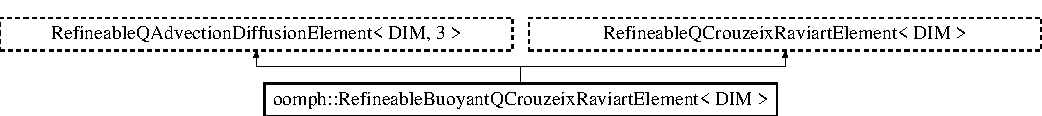
\includegraphics[height=1.166667cm]{classoomph_1_1RefineableBuoyantQCrouzeixRaviartElement}
\end{center}
\end{figure}
\subsection*{Public Member Functions}
\begin{DoxyCompactItemize}
\item 
\hyperlink{classoomph_1_1RefineableBuoyantQCrouzeixRaviartElement_a180c3373158434bc08fc69cc0f4392f9}{Refineable\+Buoyant\+Q\+Crouzeix\+Raviart\+Element} ()
\begin{DoxyCompactList}\small\item\em Constructor\+: call the underlying constructors and initialise the pointer to the Rayleigh number to address the default value of 0.\+0. \end{DoxyCompactList}\item 
unsigned \hyperlink{classoomph_1_1RefineableBuoyantQCrouzeixRaviartElement_a664008af1b7a6444cee34bd4f506c318}{required\+\_\+nvalue} (const unsigned \&n) const
\begin{DoxyCompactList}\small\item\em The required number of values stored at the nodes is the sum of the required values of the two single-\/physics elements. This step is generic for any composed element of this type. \end{DoxyCompactList}\item 
const double \& \hyperlink{classoomph_1_1RefineableBuoyantQCrouzeixRaviartElement_a56e468f0ee6553a538f6f8d460e6364e}{ra} () const
\begin{DoxyCompactList}\small\item\em Access function for the Rayleigh number (const version) \end{DoxyCompactList}\item 
double $\ast$\& \hyperlink{classoomph_1_1RefineableBuoyantQCrouzeixRaviartElement_acd96d12e3caedc1a38582079d977c0e4}{ra\+\_\+pt} ()
\begin{DoxyCompactList}\small\item\em Access function for the pointer to the Rayleigh number. \end{DoxyCompactList}\item 
void \hyperlink{classoomph_1_1RefineableBuoyantQCrouzeixRaviartElement_a7fdb84a7d69740668514e0dae2d07f7e}{disable\+\_\+\+A\+LE} ()
\begin{DoxyCompactList}\small\item\em Final override for disable A\+LE. \end{DoxyCompactList}\item 
void \hyperlink{classoomph_1_1RefineableBuoyantQCrouzeixRaviartElement_a7006ef1edd1ac4a178e38945fae581ee}{enable\+\_\+\+A\+LE} ()
\begin{DoxyCompactList}\small\item\em Final override for enable A\+LE. \end{DoxyCompactList}\item 
unsigned \hyperlink{classoomph_1_1RefineableBuoyantQCrouzeixRaviartElement_a2167093a1902a2ed4c79d45eff457ca8}{nscalar\+\_\+paraview} () const
\begin{DoxyCompactList}\small\item\em Number of scalars/fields output by this element. Broken virtual. Needs to be implemented for each new specific element type. Temporary dummy. \end{DoxyCompactList}\item 
void \hyperlink{classoomph_1_1RefineableBuoyantQCrouzeixRaviartElement_a9a8ee12b27daa327e97fbacc89c341c6}{scalar\+\_\+value\+\_\+paraview} (std\+::ofstream \&file\+\_\+out, const unsigned \&\hyperlink{cfortran_8h_adb50e893b86b3e55e751a42eab3cba82}{i}, const unsigned \&nplot) const
\begin{DoxyCompactList}\small\item\em Write values of the i-\/th scalar field at the plot points. Broken virtual. Needs to be implemented for each new specific element type. Temporary dummy. \end{DoxyCompactList}\item 
std\+::string \hyperlink{classoomph_1_1RefineableBuoyantQCrouzeixRaviartElement_ae9b9687a5a15a0089431ad1b143356e5}{scalar\+\_\+name\+\_\+paraview} (const unsigned \&\hyperlink{cfortran_8h_adb50e893b86b3e55e751a42eab3cba82}{i}) const
\begin{DoxyCompactList}\small\item\em Name of the i-\/th scalar field. Default implementation returns V1 for the first one, V2 for the second etc. Can (should!) be overloaded with more meaningful names. \end{DoxyCompactList}\item 
void \hyperlink{classoomph_1_1RefineableBuoyantQCrouzeixRaviartElement_abbe05b977edbfec7752ed417b90e09fa}{output} (std\+::ostream \&outfile)
\begin{DoxyCompactList}\small\item\em Overload the standard output function with the broken default. \end{DoxyCompactList}\item 
void \hyperlink{classoomph_1_1RefineableBuoyantQCrouzeixRaviartElement_a36bc6dc9052947f0932a605dd4d0e8f0}{output} (std\+::ostream \&outfile, const unsigned \&nplot)
\begin{DoxyCompactList}\small\item\em Output function\+: x,y,u or x,y,z,u at Nplot$^\wedge$\+D\+IM plot points. \end{DoxyCompactList}\item 
void \hyperlink{classoomph_1_1RefineableBuoyantQCrouzeixRaviartElement_a90579086f991da7fbaf7d92b29abf994}{output} (F\+I\+LE $\ast$file\+\_\+pt)
\begin{DoxyCompactList}\small\item\em C-\/style output function\+: Broken default. \end{DoxyCompactList}\item 
void \hyperlink{classoomph_1_1RefineableBuoyantQCrouzeixRaviartElement_a650e1b0428cd160c72dbc3deda287b26}{output} (F\+I\+LE $\ast$file\+\_\+pt, const unsigned \&n\+\_\+plot)
\begin{DoxyCompactList}\small\item\em C-\/style output function\+: Broken default. \end{DoxyCompactList}\item 
void \hyperlink{classoomph_1_1RefineableBuoyantQCrouzeixRaviartElement_a9f9feaf2d6003f2328741de2987fd0d1}{output\+\_\+fct} (std\+::ostream \&outfile, const unsigned \&Nplot, \hyperlink{classoomph_1_1FiniteElement_a690fd33af26cc3e84f39bba6d5a85202}{Finite\+Element\+::\+Steady\+Exact\+Solution\+Fct\+Pt} exact\+\_\+soln\+\_\+pt)
\begin{DoxyCompactList}\small\item\em Output function for an exact solution\+: Broken default. \end{DoxyCompactList}\item 
void \hyperlink{classoomph_1_1RefineableBuoyantQCrouzeixRaviartElement_aa1eaab23a14039a18701b5666629b5bc}{output\+\_\+fct} (std\+::ostream \&outfile, const unsigned \&Nplot, const double \&time, \hyperlink{classoomph_1_1FiniteElement_ad4ecf2b61b158a4b4d351a60d23c633e}{Finite\+Element\+::\+Unsteady\+Exact\+Solution\+Fct\+Pt} exact\+\_\+soln\+\_\+pt)
\begin{DoxyCompactList}\small\item\em Output function for a time-\/dependent exact solution. Broken default. \end{DoxyCompactList}\item 
unsigned \hyperlink{classoomph_1_1RefineableBuoyantQCrouzeixRaviartElement_ac6a973ee5e4d7425db2e7f9a259bab46}{u\+\_\+index\+\_\+adv\+\_\+diff} () const
\begin{DoxyCompactList}\small\item\em Overload the index at which the temperature variable is stored. We choose to store is after the fluid velocities. \end{DoxyCompactList}\item 
unsigned \hyperlink{classoomph_1_1RefineableBuoyantQCrouzeixRaviartElement_a868eb9a7f06469da529dbbc5b1efe34e}{nvertex\+\_\+node} () const
\begin{DoxyCompactList}\small\item\em Number of vertex nodes in the element is obtained from the geometric element. \end{DoxyCompactList}\item 
\hyperlink{classoomph_1_1Node}{Node} $\ast$ \hyperlink{classoomph_1_1RefineableBuoyantQCrouzeixRaviartElement_a39d79b2fe742148c2d3856ed05ad78db}{vertex\+\_\+node\+\_\+pt} (const unsigned \&j) const
\begin{DoxyCompactList}\small\item\em Pointer to the j-\/th vertex node in the element, Call the geometric element\textquotesingle{}s function. \end{DoxyCompactList}\item 
unsigned \hyperlink{classoomph_1_1RefineableBuoyantQCrouzeixRaviartElement_a98f094a1c3080905d0e90f5ac6ebd1b6}{ncont\+\_\+interpolated\+\_\+values} () const
\begin{DoxyCompactList}\small\item\em The total number of continously interpolated values is D\+I\+M+1 (D\+IM fluid velocities and one temperature). \end{DoxyCompactList}\item 
void \hyperlink{classoomph_1_1RefineableBuoyantQCrouzeixRaviartElement_aa89e116d612b3530edd2b0666d25cf01}{get\+\_\+interpolated\+\_\+values} (const \hyperlink{classoomph_1_1Vector}{Vector}$<$ double $>$ \&\hyperlink{cfortran_8h_ab7123126e4885ef647dd9c6e3807a21c}{s}, \hyperlink{classoomph_1_1Vector}{Vector}$<$ double $>$ \&values)
\begin{DoxyCompactList}\small\item\em Get the continuously interpolated values at the local coordinate s. We choose to put the fluid velocities first, followed by the temperature. \end{DoxyCompactList}\item 
void \hyperlink{classoomph_1_1RefineableBuoyantQCrouzeixRaviartElement_af178c04f0e6ee09a5d05574fcd68ac41}{get\+\_\+interpolated\+\_\+values} (const unsigned \&\hyperlink{cfortran_8h_af6f0bd3dc13317f895c91323c25c2b8f}{t}, const \hyperlink{classoomph_1_1Vector}{Vector}$<$ double $>$ \&\hyperlink{cfortran_8h_ab7123126e4885ef647dd9c6e3807a21c}{s}, \hyperlink{classoomph_1_1Vector}{Vector}$<$ double $>$ \&values)
\begin{DoxyCompactList}\small\item\em Get all continuously interpolated values at the local coordinate s at time level t (t=0\+: present; t$>$0\+: previous). We choose to put the fluid velocities first, followed by the temperature. \end{DoxyCompactList}\item 
void \hyperlink{classoomph_1_1RefineableBuoyantQCrouzeixRaviartElement_ab0a823598e014557e7d2ef2d533972d1}{further\+\_\+setup\+\_\+hanging\+\_\+nodes} ()
\begin{DoxyCompactList}\small\item\em The additional hanging node information must be set up for both single-\/physics elements. \end{DoxyCompactList}\item 
void \hyperlink{classoomph_1_1RefineableBuoyantQCrouzeixRaviartElement_a00e5ff46d718e47374a3d1dc282f419c}{rebuild\+\_\+from\+\_\+sons} (\hyperlink{classoomph_1_1Mesh}{Mesh} $\ast$\&mesh\+\_\+pt)
\begin{DoxyCompactList}\small\item\em Call the rebuild\+\_\+from\+\_\+sons functions for each of the constituent multi-\/physics elements. \end{DoxyCompactList}\item 
void \hyperlink{classoomph_1_1RefineableBuoyantQCrouzeixRaviartElement_a60d622f02595901b5f3ad830de915471}{further\+\_\+build} ()
\begin{DoxyCompactList}\small\item\em Call the underlying single-\/physics element\textquotesingle{}s \hyperlink{classoomph_1_1RefineableBuoyantQCrouzeixRaviartElement_a60d622f02595901b5f3ad830de915471}{further\+\_\+build()} functions and make sure that the pointer to the Rayleigh number is passed to the sons. \end{DoxyCompactList}\item 
unsigned \hyperlink{classoomph_1_1RefineableBuoyantQCrouzeixRaviartElement_a18e7035500add323a8d5ce921c9c1b8a}{nrecovery\+\_\+order} ()
\begin{DoxyCompactList}\small\item\em The recovery order is that of the Navier\+Stokes elements. \end{DoxyCompactList}\item 
unsigned \hyperlink{classoomph_1_1RefineableBuoyantQCrouzeixRaviartElement_a630b9aa6c5cf924d32996e89ed230175}{num\+\_\+\+Z2\+\_\+flux\+\_\+terms} ()
\begin{DoxyCompactList}\small\item\em The number of Z2 flux terms is the same as that in the fluid element plus that in the advection-\/diffusion element. \end{DoxyCompactList}\item 
void \hyperlink{classoomph_1_1RefineableBuoyantQCrouzeixRaviartElement_a1b78fb6b311b89cff1b57fcaacd924d7}{get\+\_\+\+Z2\+\_\+flux} (const \hyperlink{classoomph_1_1Vector}{Vector}$<$ double $>$ \&\hyperlink{cfortran_8h_ab7123126e4885ef647dd9c6e3807a21c}{s}, \hyperlink{classoomph_1_1Vector}{Vector}$<$ double $>$ \&flux)
\begin{DoxyCompactList}\small\item\em Get the Z2 flux by concatenating the fluxes from the fluid and the advection diffusion elements. \end{DoxyCompactList}\item 
unsigned \hyperlink{classoomph_1_1RefineableBuoyantQCrouzeixRaviartElement_a395397240c5745ad7ed66ce6f66b5d99}{ncompound\+\_\+fluxes} ()
\begin{DoxyCompactList}\small\item\em The number of compound fluxes is two (one for the fluid and one for the temperature) \end{DoxyCompactList}\item 
void \hyperlink{classoomph_1_1RefineableBuoyantQCrouzeixRaviartElement_ac8b5c8d8df0dc6d7af67570c609f591b}{get\+\_\+\+Z2\+\_\+compound\+\_\+flux\+\_\+indices} (\hyperlink{classoomph_1_1Vector}{Vector}$<$ unsigned $>$ \&flux\+\_\+index)
\begin{DoxyCompactList}\small\item\em Fill in which flux components are associated with the fluid measure and which are associated with the temperature measure. \end{DoxyCompactList}\item 
void \hyperlink{classoomph_1_1RefineableBuoyantQCrouzeixRaviartElement_ad239e9a0ebe88136d68e1521fc51e0bb}{compute\+\_\+error} (std\+::ostream \&outfile, \hyperlink{classoomph_1_1FiniteElement_ad4ecf2b61b158a4b4d351a60d23c633e}{Finite\+Element\+::\+Unsteady\+Exact\+Solution\+Fct\+Pt} exact\+\_\+soln\+\_\+pt, const double \&time, double \&error, double \&norm)
\begin{DoxyCompactList}\small\item\em Validate against exact solution at given time Solution is provided via function pointer. Plot at a given number of plot points and compute L2 error and L2 norm of velocity solution over element Overload to broken default. \end{DoxyCompactList}\item 
void \hyperlink{classoomph_1_1RefineableBuoyantQCrouzeixRaviartElement_a078039343f5f9bb467a1183f725d1873}{compute\+\_\+error} (std\+::ostream \&outfile, \hyperlink{classoomph_1_1FiniteElement_a690fd33af26cc3e84f39bba6d5a85202}{Finite\+Element\+::\+Steady\+Exact\+Solution\+Fct\+Pt} exact\+\_\+soln\+\_\+pt, double \&error, double \&norm)
\begin{DoxyCompactList}\small\item\em Validate against exact solution. Solution is provided via function pointer. Plot at a given number of plot points and compute L2 error and L2 norm of velocity solution over element Overload to broken default. \end{DoxyCompactList}\item 
void \hyperlink{classoomph_1_1RefineableBuoyantQCrouzeixRaviartElement_a093f484b86df6e7cb59d4cc9e605fb51}{get\+\_\+wind\+\_\+adv\+\_\+diff} (const unsigned \&ipt, const \hyperlink{classoomph_1_1Vector}{Vector}$<$ double $>$ \&\hyperlink{cfortran_8h_ab7123126e4885ef647dd9c6e3807a21c}{s}, const \hyperlink{classoomph_1_1Vector}{Vector}$<$ double $>$ \&x, \hyperlink{classoomph_1_1Vector}{Vector}$<$ double $>$ \&wind) const
\begin{DoxyCompactList}\small\item\em Overload the wind function in the advection-\/diffusion equations. This provides the coupling from the Navier--Stokes equations to the advection-\/diffusion equations because the wind is the fluid velocity. \end{DoxyCompactList}\item 
void \hyperlink{classoomph_1_1RefineableBuoyantQCrouzeixRaviartElement_a69fb9113989d692dd55eb1983cdbc93b}{get\+\_\+body\+\_\+force\+\_\+nst} (const double \&time, const unsigned \&ipt, const \hyperlink{classoomph_1_1Vector}{Vector}$<$ double $>$ \&\hyperlink{cfortran_8h_ab7123126e4885ef647dd9c6e3807a21c}{s}, const \hyperlink{classoomph_1_1Vector}{Vector}$<$ double $>$ \&x, \hyperlink{classoomph_1_1Vector}{Vector}$<$ double $>$ \&result)
\begin{DoxyCompactList}\small\item\em Overload the body force in the navier-\/stokes equations This provides the coupling from the advection-\/diffusion equations to the Navier--Stokes equations, the body force is the temperature multiplied by the Rayleigh number acting in the direction opposite to gravity. \end{DoxyCompactList}\item 
void \hyperlink{classoomph_1_1RefineableBuoyantQCrouzeixRaviartElement_a102b3aeb79d9af430b9ce0a7c8d5bd33}{fill\+\_\+in\+\_\+contribution\+\_\+to\+\_\+residuals} (\hyperlink{classoomph_1_1Vector}{Vector}$<$ double $>$ \&residuals)
\begin{DoxyCompactList}\small\item\em Fill in the constituent elements\textquotesingle{} contribution to the residual vector. \end{DoxyCompactList}\item 
void \hyperlink{classoomph_1_1RefineableBuoyantQCrouzeixRaviartElement_a0d05a727999c7f102f3fe2bacce38f6b}{fill\+\_\+in\+\_\+contribution\+\_\+to\+\_\+jacobian} (\hyperlink{classoomph_1_1Vector}{Vector}$<$ double $>$ \&residuals, \hyperlink{classoomph_1_1DenseMatrix}{Dense\+Matrix}$<$ double $>$ \&jacobian)
\begin{DoxyCompactList}\small\item\em Compute the element\textquotesingle{}s residual \hyperlink{classoomph_1_1Vector}{Vector} and the jacobian matrix using full finite differences, the default implementation. \end{DoxyCompactList}\item 
void \hyperlink{classoomph_1_1RefineableBuoyantQCrouzeixRaviartElement_a06f1e2dbdf7a8ebaa964d421aee453ee}{fill\+\_\+in\+\_\+contribution\+\_\+to\+\_\+jacobian\+\_\+and\+\_\+mass\+\_\+matrix} (\hyperlink{classoomph_1_1Vector}{Vector}$<$ double $>$ \&residuals, \hyperlink{classoomph_1_1DenseMatrix}{Dense\+Matrix}$<$ double $>$ \&jacobian, \hyperlink{classoomph_1_1DenseMatrix}{Dense\+Matrix}$<$ double $>$ \&mass\+\_\+matrix)
\item 
void \hyperlink{classoomph_1_1RefineableBuoyantQCrouzeixRaviartElement_a6fe93946149c696f273be12540099d1a}{fill\+\_\+in\+\_\+off\+\_\+diagonal\+\_\+jacobian\+\_\+blocks\+\_\+analytic} (\hyperlink{classoomph_1_1Vector}{Vector}$<$ double $>$ \&residuals, \hyperlink{classoomph_1_1DenseMatrix}{Dense\+Matrix}$<$ double $>$ \&jacobian)
\begin{DoxyCompactList}\small\item\em Compute the contribution of the off-\/diagonal blocks analytically. \end{DoxyCompactList}\end{DoxyCompactItemize}
\subsection*{Private Member Functions}
\begin{DoxyCompactItemize}
\item 
{\footnotesize template$<$$>$ }\\double \hyperlink{classoomph_1_1RefineableBuoyantQCrouzeixRaviartElement_ab36052eddfa043777414ce64470bb0a3}{Default\+\_\+\+Physical\+\_\+\+Constant\+\_\+\+Value}
\begin{DoxyCompactList}\small\item\em Set the default value of the Rayleigh number to be zero. \end{DoxyCompactList}\item 
{\footnotesize template$<$$>$ }\\double \hyperlink{classoomph_1_1RefineableBuoyantQCrouzeixRaviartElement_a4e22ae2489586ac69c1e5ebcb04e6343}{Default\+\_\+\+Physical\+\_\+\+Constant\+\_\+\+Value}
\end{DoxyCompactItemize}
\subsection*{Private Attributes}
\begin{DoxyCompactItemize}
\item 
double $\ast$ \hyperlink{classoomph_1_1RefineableBuoyantQCrouzeixRaviartElement_a65ce0c55087be240fc183e08def8b07b}{Ra\+\_\+pt}
\begin{DoxyCompactList}\small\item\em Pointer to a new physical variable, the Rayleigh number. \end{DoxyCompactList}\end{DoxyCompactItemize}
\subsection*{Static Private Attributes}
\begin{DoxyCompactItemize}
\item 
static double \hyperlink{classoomph_1_1RefineableBuoyantQCrouzeixRaviartElement_a33bf1cb8ad42fc6418e71acabbe1925e}{Default\+\_\+\+Physical\+\_\+\+Constant\+\_\+\+Value}
\begin{DoxyCompactList}\small\item\em The static default value of the Rayleigh number. \end{DoxyCompactList}\end{DoxyCompactItemize}
\subsection*{Additional Inherited Members}


\subsection{Detailed Description}
\subsubsection*{template$<$unsigned D\+IM$>$\newline
class oomph\+::\+Refineable\+Buoyant\+Q\+Crouzeix\+Raviart\+Element$<$ D\+I\+M $>$}

A \hyperlink{classoomph_1_1RefineableElement}{Refineable\+Element} class that solves the Boussinesq approximation of the Navier--Stokes and energy equations by coupling two pre-\/existing classes. The \hyperlink{classoomph_1_1RefineableQAdvectionDiffusionElement}{Refineable\+Q\+Advection\+Diffusion\+Element} with bi-\/quadratic interpolation for the scalar variable (temperature) and \hyperlink{classoomph_1_1RefineableQCrouzeixRaviartElement}{Refineable\+Q\+Crouzeix\+Raviart\+Element} which solves the Navier--Stokes equations using bi-\/quadratic interpolation for the velocities and a discontinuous bi-\/linear interpolation for the pressure. Note that we are free to choose the order in which we store the variables at the nodes. In this case we choose to store the variables in the order fluid velocities followed by temperature. We must, therefore, overload the function \hyperlink{classoomph_1_1AdvectionDiffusionEquations_aadffa26c42be5d4a1156a7467de48fb8}{Advection\+Diffusion\+Equations$<$\+D\+I\+M$>$\+::u\+\_\+index\+\_\+adv\+\_\+diff()} to indicate that the temperature is stored at the D\+I\+M-\/th position not the 0-\/th. We do not need to overload the corresponding function in the Navier\+Stokes\+Equations$<$\+D\+I\+M$>$ class because the velocities are stored first. Finally, we choose to use the flux-\/recovery calculation from the fluid velocities to provide the error used in the mesh adaptation. 

Definition at line 759 of file boussinesq\+\_\+elements.\+h.



\subsection{Constructor \& Destructor Documentation}
\mbox{\Hypertarget{classoomph_1_1RefineableBuoyantQCrouzeixRaviartElement_a180c3373158434bc08fc69cc0f4392f9}\label{classoomph_1_1RefineableBuoyantQCrouzeixRaviartElement_a180c3373158434bc08fc69cc0f4392f9}} 
\index{oomph\+::\+Refineable\+Buoyant\+Q\+Crouzeix\+Raviart\+Element@{oomph\+::\+Refineable\+Buoyant\+Q\+Crouzeix\+Raviart\+Element}!Refineable\+Buoyant\+Q\+Crouzeix\+Raviart\+Element@{Refineable\+Buoyant\+Q\+Crouzeix\+Raviart\+Element}}
\index{Refineable\+Buoyant\+Q\+Crouzeix\+Raviart\+Element@{Refineable\+Buoyant\+Q\+Crouzeix\+Raviart\+Element}!oomph\+::\+Refineable\+Buoyant\+Q\+Crouzeix\+Raviart\+Element@{oomph\+::\+Refineable\+Buoyant\+Q\+Crouzeix\+Raviart\+Element}}
\subsubsection{\texorpdfstring{Refineable\+Buoyant\+Q\+Crouzeix\+Raviart\+Element()}{RefineableBuoyantQCrouzeixRaviartElement()}}
{\footnotesize\ttfamily template$<$unsigned D\+IM$>$ \\
\hyperlink{classoomph_1_1RefineableBuoyantQCrouzeixRaviartElement}{oomph\+::\+Refineable\+Buoyant\+Q\+Crouzeix\+Raviart\+Element}$<$ D\+IM $>$\+::\hyperlink{classoomph_1_1RefineableBuoyantQCrouzeixRaviartElement}{Refineable\+Buoyant\+Q\+Crouzeix\+Raviart\+Element} (\begin{DoxyParamCaption}{ }\end{DoxyParamCaption})\hspace{0.3cm}{\ttfamily [inline]}}



Constructor\+: call the underlying constructors and initialise the pointer to the Rayleigh number to address the default value of 0.\+0. 



Definition at line 776 of file boussinesq\+\_\+elements.\+h.



References oomph\+::\+Buoyant\+Q\+Crouzeix\+Raviart\+Element$<$ D\+I\+M $>$\+::\+Default\+\_\+\+Physical\+\_\+\+Constant\+\_\+\+Value().



\subsection{Member Function Documentation}
\mbox{\Hypertarget{classoomph_1_1RefineableBuoyantQCrouzeixRaviartElement_ad239e9a0ebe88136d68e1521fc51e0bb}\label{classoomph_1_1RefineableBuoyantQCrouzeixRaviartElement_ad239e9a0ebe88136d68e1521fc51e0bb}} 
\index{oomph\+::\+Refineable\+Buoyant\+Q\+Crouzeix\+Raviart\+Element@{oomph\+::\+Refineable\+Buoyant\+Q\+Crouzeix\+Raviart\+Element}!compute\+\_\+error@{compute\+\_\+error}}
\index{compute\+\_\+error@{compute\+\_\+error}!oomph\+::\+Refineable\+Buoyant\+Q\+Crouzeix\+Raviart\+Element@{oomph\+::\+Refineable\+Buoyant\+Q\+Crouzeix\+Raviart\+Element}}
\subsubsection{\texorpdfstring{compute\+\_\+error()}{compute\_error()}\hspace{0.1cm}{\footnotesize\ttfamily [1/2]}}
{\footnotesize\ttfamily template$<$unsigned D\+IM$>$ \\
void \hyperlink{classoomph_1_1RefineableBuoyantQCrouzeixRaviartElement}{oomph\+::\+Refineable\+Buoyant\+Q\+Crouzeix\+Raviart\+Element}$<$ D\+IM $>$\+::compute\+\_\+error (\begin{DoxyParamCaption}\item[{std\+::ostream \&}]{outfile,  }\item[{\hyperlink{classoomph_1_1FiniteElement_ad4ecf2b61b158a4b4d351a60d23c633e}{Finite\+Element\+::\+Unsteady\+Exact\+Solution\+Fct\+Pt}}]{exact\+\_\+soln\+\_\+pt,  }\item[{const double \&}]{time,  }\item[{double \&}]{error,  }\item[{double \&}]{norm }\end{DoxyParamCaption})\hspace{0.3cm}{\ttfamily [inline]}, {\ttfamily [virtual]}}



Validate against exact solution at given time Solution is provided via function pointer. Plot at a given number of plot points and compute L2 error and L2 norm of velocity solution over element Overload to broken default. 



Reimplemented from \hyperlink{classoomph_1_1AdvectionDiffusionEquations_a87c8c4e8ff5ea6e6dcb243ec83bb4fd2}{oomph\+::\+Advection\+Diffusion\+Equations$<$ D\+I\+M $>$}.



Definition at line 1110 of file boussinesq\+\_\+elements.\+h.



References oomph\+::\+Finite\+Element\+::compute\+\_\+error().

\mbox{\Hypertarget{classoomph_1_1RefineableBuoyantQCrouzeixRaviartElement_a078039343f5f9bb467a1183f725d1873}\label{classoomph_1_1RefineableBuoyantQCrouzeixRaviartElement_a078039343f5f9bb467a1183f725d1873}} 
\index{oomph\+::\+Refineable\+Buoyant\+Q\+Crouzeix\+Raviart\+Element@{oomph\+::\+Refineable\+Buoyant\+Q\+Crouzeix\+Raviart\+Element}!compute\+\_\+error@{compute\+\_\+error}}
\index{compute\+\_\+error@{compute\+\_\+error}!oomph\+::\+Refineable\+Buoyant\+Q\+Crouzeix\+Raviart\+Element@{oomph\+::\+Refineable\+Buoyant\+Q\+Crouzeix\+Raviart\+Element}}
\subsubsection{\texorpdfstring{compute\+\_\+error()}{compute\_error()}\hspace{0.1cm}{\footnotesize\ttfamily [2/2]}}
{\footnotesize\ttfamily template$<$unsigned D\+IM$>$ \\
void \hyperlink{classoomph_1_1RefineableBuoyantQCrouzeixRaviartElement}{oomph\+::\+Refineable\+Buoyant\+Q\+Crouzeix\+Raviart\+Element}$<$ D\+IM $>$\+::compute\+\_\+error (\begin{DoxyParamCaption}\item[{std\+::ostream \&}]{outfile,  }\item[{\hyperlink{classoomph_1_1FiniteElement_a690fd33af26cc3e84f39bba6d5a85202}{Finite\+Element\+::\+Steady\+Exact\+Solution\+Fct\+Pt}}]{exact\+\_\+soln\+\_\+pt,  }\item[{double \&}]{error,  }\item[{double \&}]{norm }\end{DoxyParamCaption})\hspace{0.3cm}{\ttfamily [inline]}, {\ttfamily [virtual]}}



Validate against exact solution. Solution is provided via function pointer. Plot at a given number of plot points and compute L2 error and L2 norm of velocity solution over element Overload to broken default. 



Reimplemented from \hyperlink{classoomph_1_1AdvectionDiffusionEquations_acb1fcfb29911210ad7c0bc252f0ed665}{oomph\+::\+Advection\+Diffusion\+Equations$<$ D\+I\+M $>$}.



Definition at line 1122 of file boussinesq\+\_\+elements.\+h.



References oomph\+::\+Finite\+Element\+::compute\+\_\+error().

\mbox{\Hypertarget{classoomph_1_1RefineableBuoyantQCrouzeixRaviartElement_ab36052eddfa043777414ce64470bb0a3}\label{classoomph_1_1RefineableBuoyantQCrouzeixRaviartElement_ab36052eddfa043777414ce64470bb0a3}} 
\index{oomph\+::\+Refineable\+Buoyant\+Q\+Crouzeix\+Raviart\+Element@{oomph\+::\+Refineable\+Buoyant\+Q\+Crouzeix\+Raviart\+Element}!Default\+\_\+\+Physical\+\_\+\+Constant\+\_\+\+Value@{Default\+\_\+\+Physical\+\_\+\+Constant\+\_\+\+Value}}
\index{Default\+\_\+\+Physical\+\_\+\+Constant\+\_\+\+Value@{Default\+\_\+\+Physical\+\_\+\+Constant\+\_\+\+Value}!oomph\+::\+Refineable\+Buoyant\+Q\+Crouzeix\+Raviart\+Element@{oomph\+::\+Refineable\+Buoyant\+Q\+Crouzeix\+Raviart\+Element}}
\subsubsection{\texorpdfstring{Default\+\_\+\+Physical\+\_\+\+Constant\+\_\+\+Value()}{Default\_Physical\_Constant\_Value()}\hspace{0.1cm}{\footnotesize\ttfamily [1/2]}}
{\footnotesize\ttfamily template$<$$>$ \\
double \hyperlink{classoomph_1_1RefineableBuoyantQCrouzeixRaviartElement}{oomph\+::\+Refineable\+Buoyant\+Q\+Crouzeix\+Raviart\+Element}$<$ 2 $>$\+::Default\+\_\+\+Physical\+\_\+\+Constant\+\_\+\+Value (\begin{DoxyParamCaption}{ }\end{DoxyParamCaption})\hspace{0.3cm}{\ttfamily [private]}}



Set the default value of the Rayleigh number to be zero. 



Definition at line 1500 of file boussinesq\+\_\+elements.\+h.

\mbox{\Hypertarget{classoomph_1_1RefineableBuoyantQCrouzeixRaviartElement_a4e22ae2489586ac69c1e5ebcb04e6343}\label{classoomph_1_1RefineableBuoyantQCrouzeixRaviartElement_a4e22ae2489586ac69c1e5ebcb04e6343}} 
\index{oomph\+::\+Refineable\+Buoyant\+Q\+Crouzeix\+Raviart\+Element@{oomph\+::\+Refineable\+Buoyant\+Q\+Crouzeix\+Raviart\+Element}!Default\+\_\+\+Physical\+\_\+\+Constant\+\_\+\+Value@{Default\+\_\+\+Physical\+\_\+\+Constant\+\_\+\+Value}}
\index{Default\+\_\+\+Physical\+\_\+\+Constant\+\_\+\+Value@{Default\+\_\+\+Physical\+\_\+\+Constant\+\_\+\+Value}!oomph\+::\+Refineable\+Buoyant\+Q\+Crouzeix\+Raviart\+Element@{oomph\+::\+Refineable\+Buoyant\+Q\+Crouzeix\+Raviart\+Element}}
\subsubsection{\texorpdfstring{Default\+\_\+\+Physical\+\_\+\+Constant\+\_\+\+Value()}{Default\_Physical\_Constant\_Value()}\hspace{0.1cm}{\footnotesize\ttfamily [2/2]}}
{\footnotesize\ttfamily template$<$$>$ \\
double \hyperlink{classoomph_1_1RefineableBuoyantQCrouzeixRaviartElement}{oomph\+::\+Refineable\+Buoyant\+Q\+Crouzeix\+Raviart\+Element}$<$ 3 $>$\+::Default\+\_\+\+Physical\+\_\+\+Constant\+\_\+\+Value (\begin{DoxyParamCaption}{ }\end{DoxyParamCaption})\hspace{0.3cm}{\ttfamily [private]}}



Definition at line 1504 of file boussinesq\+\_\+elements.\+h.

\mbox{\Hypertarget{classoomph_1_1RefineableBuoyantQCrouzeixRaviartElement_a7fdb84a7d69740668514e0dae2d07f7e}\label{classoomph_1_1RefineableBuoyantQCrouzeixRaviartElement_a7fdb84a7d69740668514e0dae2d07f7e}} 
\index{oomph\+::\+Refineable\+Buoyant\+Q\+Crouzeix\+Raviart\+Element@{oomph\+::\+Refineable\+Buoyant\+Q\+Crouzeix\+Raviart\+Element}!disable\+\_\+\+A\+LE@{disable\+\_\+\+A\+LE}}
\index{disable\+\_\+\+A\+LE@{disable\+\_\+\+A\+LE}!oomph\+::\+Refineable\+Buoyant\+Q\+Crouzeix\+Raviart\+Element@{oomph\+::\+Refineable\+Buoyant\+Q\+Crouzeix\+Raviart\+Element}}
\subsubsection{\texorpdfstring{disable\+\_\+\+A\+L\+E()}{disable\_ALE()}}
{\footnotesize\ttfamily template$<$unsigned D\+IM$>$ \\
void \hyperlink{classoomph_1_1RefineableBuoyantQCrouzeixRaviartElement}{oomph\+::\+Refineable\+Buoyant\+Q\+Crouzeix\+Raviart\+Element}$<$ D\+IM $>$\+::disable\+\_\+\+A\+LE (\begin{DoxyParamCaption}{ }\end{DoxyParamCaption})\hspace{0.3cm}{\ttfamily [inline]}, {\ttfamily [virtual]}}



Final override for disable A\+LE. 



Reimplemented from \hyperlink{classoomph_1_1AdvectionDiffusionEquations_aa635388e5e1139e0a1eae97ca89279d0}{oomph\+::\+Advection\+Diffusion\+Equations$<$ D\+I\+M $>$}.



Definition at line 798 of file boussinesq\+\_\+elements.\+h.



References oomph\+::\+Advection\+Diffusion\+Equations$<$ D\+I\+M $>$\+::disable\+\_\+\+A\+L\+E(), and oomph\+::\+Navier\+Stokes\+Equations$<$ D\+I\+M $>$\+::disable\+\_\+\+A\+L\+E().

\mbox{\Hypertarget{classoomph_1_1RefineableBuoyantQCrouzeixRaviartElement_a7006ef1edd1ac4a178e38945fae581ee}\label{classoomph_1_1RefineableBuoyantQCrouzeixRaviartElement_a7006ef1edd1ac4a178e38945fae581ee}} 
\index{oomph\+::\+Refineable\+Buoyant\+Q\+Crouzeix\+Raviart\+Element@{oomph\+::\+Refineable\+Buoyant\+Q\+Crouzeix\+Raviart\+Element}!enable\+\_\+\+A\+LE@{enable\+\_\+\+A\+LE}}
\index{enable\+\_\+\+A\+LE@{enable\+\_\+\+A\+LE}!oomph\+::\+Refineable\+Buoyant\+Q\+Crouzeix\+Raviart\+Element@{oomph\+::\+Refineable\+Buoyant\+Q\+Crouzeix\+Raviart\+Element}}
\subsubsection{\texorpdfstring{enable\+\_\+\+A\+L\+E()}{enable\_ALE()}}
{\footnotesize\ttfamily template$<$unsigned D\+IM$>$ \\
void \hyperlink{classoomph_1_1RefineableBuoyantQCrouzeixRaviartElement}{oomph\+::\+Refineable\+Buoyant\+Q\+Crouzeix\+Raviart\+Element}$<$ D\+IM $>$\+::enable\+\_\+\+A\+LE (\begin{DoxyParamCaption}{ }\end{DoxyParamCaption})\hspace{0.3cm}{\ttfamily [inline]}, {\ttfamily [virtual]}}



Final override for enable A\+LE. 



Reimplemented from \hyperlink{classoomph_1_1AdvectionDiffusionEquations_a949dd5a3eb9803c993c1f4506cfd5d82}{oomph\+::\+Advection\+Diffusion\+Equations$<$ D\+I\+M $>$}.



Definition at line 806 of file boussinesq\+\_\+elements.\+h.



References oomph\+::\+Advection\+Diffusion\+Equations$<$ D\+I\+M $>$\+::enable\+\_\+\+A\+L\+E(), and oomph\+::\+Navier\+Stokes\+Equations$<$ D\+I\+M $>$\+::enable\+\_\+\+A\+L\+E().

\mbox{\Hypertarget{classoomph_1_1RefineableBuoyantQCrouzeixRaviartElement_a0d05a727999c7f102f3fe2bacce38f6b}\label{classoomph_1_1RefineableBuoyantQCrouzeixRaviartElement_a0d05a727999c7f102f3fe2bacce38f6b}} 
\index{oomph\+::\+Refineable\+Buoyant\+Q\+Crouzeix\+Raviart\+Element@{oomph\+::\+Refineable\+Buoyant\+Q\+Crouzeix\+Raviart\+Element}!fill\+\_\+in\+\_\+contribution\+\_\+to\+\_\+jacobian@{fill\+\_\+in\+\_\+contribution\+\_\+to\+\_\+jacobian}}
\index{fill\+\_\+in\+\_\+contribution\+\_\+to\+\_\+jacobian@{fill\+\_\+in\+\_\+contribution\+\_\+to\+\_\+jacobian}!oomph\+::\+Refineable\+Buoyant\+Q\+Crouzeix\+Raviart\+Element@{oomph\+::\+Refineable\+Buoyant\+Q\+Crouzeix\+Raviart\+Element}}
\subsubsection{\texorpdfstring{fill\+\_\+in\+\_\+contribution\+\_\+to\+\_\+jacobian()}{fill\_in\_contribution\_to\_jacobian()}}
{\footnotesize\ttfamily template$<$unsigned D\+IM$>$ \\
void \hyperlink{classoomph_1_1RefineableBuoyantQCrouzeixRaviartElement}{oomph\+::\+Refineable\+Buoyant\+Q\+Crouzeix\+Raviart\+Element}$<$ D\+IM $>$\+::fill\+\_\+in\+\_\+contribution\+\_\+to\+\_\+jacobian (\begin{DoxyParamCaption}\item[{\hyperlink{classoomph_1_1Vector}{Vector}$<$ double $>$ \&}]{residuals,  }\item[{\hyperlink{classoomph_1_1DenseMatrix}{Dense\+Matrix}$<$ double $>$ \&}]{jacobian }\end{DoxyParamCaption})\hspace{0.3cm}{\ttfamily [inline]}, {\ttfamily [virtual]}}



Compute the element\textquotesingle{}s residual \hyperlink{classoomph_1_1Vector}{Vector} and the jacobian matrix using full finite differences, the default implementation. 



Reimplemented from \hyperlink{classoomph_1_1AdvectionDiffusionEquations_a6ec1e0f92fa79998be9340ecfda4bcd5}{oomph\+::\+Advection\+Diffusion\+Equations$<$ D\+I\+M $>$}.



Definition at line 1178 of file boussinesq\+\_\+elements.\+h.



References oomph\+::\+Advection\+Diffusion\+Equations$<$ D\+I\+M $>$\+::fill\+\_\+in\+\_\+contribution\+\_\+to\+\_\+jacobian(), oomph\+::\+Navier\+Stokes\+Equations$<$ D\+I\+M $>$\+::fill\+\_\+in\+\_\+contribution\+\_\+to\+\_\+jacobian(), oomph\+::\+Finite\+Element\+::fill\+\_\+in\+\_\+contribution\+\_\+to\+\_\+jacobian(), and oomph\+::\+Buoyant\+Q\+Crouzeix\+Raviart\+Element$<$ D\+I\+M $>$\+::fill\+\_\+in\+\_\+off\+\_\+diagonal\+\_\+jacobian\+\_\+blocks\+\_\+analytic().

\mbox{\Hypertarget{classoomph_1_1RefineableBuoyantQCrouzeixRaviartElement_a06f1e2dbdf7a8ebaa964d421aee453ee}\label{classoomph_1_1RefineableBuoyantQCrouzeixRaviartElement_a06f1e2dbdf7a8ebaa964d421aee453ee}} 
\index{oomph\+::\+Refineable\+Buoyant\+Q\+Crouzeix\+Raviart\+Element@{oomph\+::\+Refineable\+Buoyant\+Q\+Crouzeix\+Raviart\+Element}!fill\+\_\+in\+\_\+contribution\+\_\+to\+\_\+jacobian\+\_\+and\+\_\+mass\+\_\+matrix@{fill\+\_\+in\+\_\+contribution\+\_\+to\+\_\+jacobian\+\_\+and\+\_\+mass\+\_\+matrix}}
\index{fill\+\_\+in\+\_\+contribution\+\_\+to\+\_\+jacobian\+\_\+and\+\_\+mass\+\_\+matrix@{fill\+\_\+in\+\_\+contribution\+\_\+to\+\_\+jacobian\+\_\+and\+\_\+mass\+\_\+matrix}!oomph\+::\+Refineable\+Buoyant\+Q\+Crouzeix\+Raviart\+Element@{oomph\+::\+Refineable\+Buoyant\+Q\+Crouzeix\+Raviart\+Element}}
\subsubsection{\texorpdfstring{fill\+\_\+in\+\_\+contribution\+\_\+to\+\_\+jacobian\+\_\+and\+\_\+mass\+\_\+matrix()}{fill\_in\_contribution\_to\_jacobian\_and\_mass\_matrix()}}
{\footnotesize\ttfamily template$<$unsigned D\+IM$>$ \\
void \hyperlink{classoomph_1_1RefineableBuoyantQCrouzeixRaviartElement}{oomph\+::\+Refineable\+Buoyant\+Q\+Crouzeix\+Raviart\+Element}$<$ D\+IM $>$\+::fill\+\_\+in\+\_\+contribution\+\_\+to\+\_\+jacobian\+\_\+and\+\_\+mass\+\_\+matrix (\begin{DoxyParamCaption}\item[{\hyperlink{classoomph_1_1Vector}{Vector}$<$ double $>$ \&}]{residuals,  }\item[{\hyperlink{classoomph_1_1DenseMatrix}{Dense\+Matrix}$<$ double $>$ \&}]{jacobian,  }\item[{\hyperlink{classoomph_1_1DenseMatrix}{Dense\+Matrix}$<$ double $>$ \&}]{mass\+\_\+matrix }\end{DoxyParamCaption})\hspace{0.3cm}{\ttfamily [inline]}, {\ttfamily [virtual]}}

Add the element\textquotesingle{}s contribution to its residuals vector, jacobian matrix and mass matrix 

Reimplemented from \hyperlink{classoomph_1_1AdvectionDiffusionEquations_aed50fe00556434c01bc855766edeb564}{oomph\+::\+Advection\+Diffusion\+Equations$<$ D\+I\+M $>$}.



Definition at line 1200 of file boussinesq\+\_\+elements.\+h.



References oomph\+::\+Generalised\+Element\+::fill\+\_\+in\+\_\+contribution\+\_\+to\+\_\+jacobian\+\_\+and\+\_\+mass\+\_\+matrix().

\mbox{\Hypertarget{classoomph_1_1RefineableBuoyantQCrouzeixRaviartElement_a102b3aeb79d9af430b9ce0a7c8d5bd33}\label{classoomph_1_1RefineableBuoyantQCrouzeixRaviartElement_a102b3aeb79d9af430b9ce0a7c8d5bd33}} 
\index{oomph\+::\+Refineable\+Buoyant\+Q\+Crouzeix\+Raviart\+Element@{oomph\+::\+Refineable\+Buoyant\+Q\+Crouzeix\+Raviart\+Element}!fill\+\_\+in\+\_\+contribution\+\_\+to\+\_\+residuals@{fill\+\_\+in\+\_\+contribution\+\_\+to\+\_\+residuals}}
\index{fill\+\_\+in\+\_\+contribution\+\_\+to\+\_\+residuals@{fill\+\_\+in\+\_\+contribution\+\_\+to\+\_\+residuals}!oomph\+::\+Refineable\+Buoyant\+Q\+Crouzeix\+Raviart\+Element@{oomph\+::\+Refineable\+Buoyant\+Q\+Crouzeix\+Raviart\+Element}}
\subsubsection{\texorpdfstring{fill\+\_\+in\+\_\+contribution\+\_\+to\+\_\+residuals()}{fill\_in\_contribution\_to\_residuals()}}
{\footnotesize\ttfamily template$<$unsigned D\+IM$>$ \\
void \hyperlink{classoomph_1_1RefineableBuoyantQCrouzeixRaviartElement}{oomph\+::\+Refineable\+Buoyant\+Q\+Crouzeix\+Raviart\+Element}$<$ D\+IM $>$\+::fill\+\_\+in\+\_\+contribution\+\_\+to\+\_\+residuals (\begin{DoxyParamCaption}\item[{\hyperlink{classoomph_1_1Vector}{Vector}$<$ double $>$ \&}]{residuals }\end{DoxyParamCaption})\hspace{0.3cm}{\ttfamily [inline]}, {\ttfamily [virtual]}}



Fill in the constituent elements\textquotesingle{} contribution to the residual vector. 



Reimplemented from \hyperlink{classoomph_1_1AdvectionDiffusionEquations_ae56ee6b085c75be438a598244c527fb5}{oomph\+::\+Advection\+Diffusion\+Equations$<$ D\+I\+M $>$}.



Definition at line 1164 of file boussinesq\+\_\+elements.\+h.



References oomph\+::\+Advection\+Diffusion\+Equations$<$ D\+I\+M $>$\+::fill\+\_\+in\+\_\+contribution\+\_\+to\+\_\+residuals(), and oomph\+::\+Navier\+Stokes\+Equations$<$ D\+I\+M $>$\+::fill\+\_\+in\+\_\+contribution\+\_\+to\+\_\+residuals().

\mbox{\Hypertarget{classoomph_1_1RefineableBuoyantQCrouzeixRaviartElement_a6fe93946149c696f273be12540099d1a}\label{classoomph_1_1RefineableBuoyantQCrouzeixRaviartElement_a6fe93946149c696f273be12540099d1a}} 
\index{oomph\+::\+Refineable\+Buoyant\+Q\+Crouzeix\+Raviart\+Element@{oomph\+::\+Refineable\+Buoyant\+Q\+Crouzeix\+Raviart\+Element}!fill\+\_\+in\+\_\+off\+\_\+diagonal\+\_\+jacobian\+\_\+blocks\+\_\+analytic@{fill\+\_\+in\+\_\+off\+\_\+diagonal\+\_\+jacobian\+\_\+blocks\+\_\+analytic}}
\index{fill\+\_\+in\+\_\+off\+\_\+diagonal\+\_\+jacobian\+\_\+blocks\+\_\+analytic@{fill\+\_\+in\+\_\+off\+\_\+diagonal\+\_\+jacobian\+\_\+blocks\+\_\+analytic}!oomph\+::\+Refineable\+Buoyant\+Q\+Crouzeix\+Raviart\+Element@{oomph\+::\+Refineable\+Buoyant\+Q\+Crouzeix\+Raviart\+Element}}
\subsubsection{\texorpdfstring{fill\+\_\+in\+\_\+off\+\_\+diagonal\+\_\+jacobian\+\_\+blocks\+\_\+analytic()}{fill\_in\_off\_diagonal\_jacobian\_blocks\_analytic()}}
{\footnotesize\ttfamily template$<$unsigned D\+IM$>$ \\
void \hyperlink{classoomph_1_1RefineableBuoyantQCrouzeixRaviartElement}{oomph\+::\+Refineable\+Buoyant\+Q\+Crouzeix\+Raviart\+Element}$<$ D\+IM $>$\+::fill\+\_\+in\+\_\+off\+\_\+diagonal\+\_\+jacobian\+\_\+blocks\+\_\+analytic (\begin{DoxyParamCaption}\item[{\hyperlink{classoomph_1_1Vector}{Vector}$<$ double $>$ \&}]{residuals,  }\item[{\hyperlink{classoomph_1_1DenseMatrix}{Dense\+Matrix}$<$ double $>$ \&}]{jacobian }\end{DoxyParamCaption})\hspace{0.3cm}{\ttfamily [inline]}}



Compute the contribution of the off-\/diagonal blocks analytically. 



Definition at line 1211 of file boussinesq\+\_\+elements.\+h.



References oomph\+::\+Buoyant\+Q\+Crouzeix\+Raviart\+Element$<$ D\+I\+M $>$\+::\+Default\+\_\+\+Physical\+\_\+\+Constant\+\_\+\+Value(), oomph\+::\+Q\+Crouzeix\+Raviart\+Element$<$ D\+I\+M $>$\+::dshape\+\_\+and\+\_\+dtest\+\_\+eulerian\+\_\+at\+\_\+knot\+\_\+nst(), oomph\+::\+Navier\+Stokes\+Equations$<$ D\+I\+M $>$\+::g(), oomph\+::\+Node\+::hanging\+\_\+pt(), i, oomph\+::\+Finite\+Element\+::integral\+\_\+pt(), oomph\+::\+Node\+::is\+\_\+hanging(), oomph\+::\+Hang\+Info\+::master\+\_\+node\+\_\+pt(), oomph\+::\+Hang\+Info\+::master\+\_\+weight(), oomph\+::\+Hang\+Info\+::nmaster(), oomph\+::\+Finite\+Element\+::nnode(), oomph\+::\+Finite\+Element\+::nodal\+\_\+local\+\_\+eqn(), oomph\+::\+Finite\+Element\+::nodal\+\_\+value(), oomph\+::\+Finite\+Element\+::node\+\_\+pt(), oomph\+::\+Integral\+::nweight(), oomph\+::\+Advection\+Diffusion\+Equations$<$ D\+I\+M $>$\+::pe(), oomph\+::\+Buoyant\+Q\+Crouzeix\+Raviart\+Element$<$ D\+I\+M $>$\+::ra(), oomph\+::\+Buoyant\+Q\+Crouzeix\+Raviart\+Element$<$ D\+I\+M $>$\+::u\+\_\+index\+\_\+adv\+\_\+diff(), oomph\+::\+Navier\+Stokes\+Equations$<$ D\+I\+M $>$\+::u\+\_\+index\+\_\+nst(), oomph\+::\+Quad\+Tree\+Names\+::W, and oomph\+::\+Integral\+::weight().

\mbox{\Hypertarget{classoomph_1_1RefineableBuoyantQCrouzeixRaviartElement_a60d622f02595901b5f3ad830de915471}\label{classoomph_1_1RefineableBuoyantQCrouzeixRaviartElement_a60d622f02595901b5f3ad830de915471}} 
\index{oomph\+::\+Refineable\+Buoyant\+Q\+Crouzeix\+Raviart\+Element@{oomph\+::\+Refineable\+Buoyant\+Q\+Crouzeix\+Raviart\+Element}!further\+\_\+build@{further\+\_\+build}}
\index{further\+\_\+build@{further\+\_\+build}!oomph\+::\+Refineable\+Buoyant\+Q\+Crouzeix\+Raviart\+Element@{oomph\+::\+Refineable\+Buoyant\+Q\+Crouzeix\+Raviart\+Element}}
\subsubsection{\texorpdfstring{further\+\_\+build()}{further\_build()}}
{\footnotesize\ttfamily template$<$unsigned D\+IM$>$ \\
void \hyperlink{classoomph_1_1RefineableBuoyantQCrouzeixRaviartElement}{oomph\+::\+Refineable\+Buoyant\+Q\+Crouzeix\+Raviart\+Element}$<$ D\+IM $>$\+::further\+\_\+build (\begin{DoxyParamCaption}{ }\end{DoxyParamCaption})\hspace{0.3cm}{\ttfamily [inline]}, {\ttfamily [virtual]}}



Call the underlying single-\/physics element\textquotesingle{}s \hyperlink{classoomph_1_1RefineableBuoyantQCrouzeixRaviartElement_a60d622f02595901b5f3ad830de915471}{further\+\_\+build()} functions and make sure that the pointer to the Rayleigh number is passed to the sons. 



Reimplemented from \hyperlink{classoomph_1_1RefineableAdvectionDiffusionEquations_a093f39b8be3671828b7018b1f6103c68}{oomph\+::\+Refineable\+Advection\+Diffusion\+Equations$<$ D\+I\+M $>$}.



Definition at line 1021 of file boussinesq\+\_\+elements.\+h.



References oomph\+::\+Refineable\+Advection\+Diffusion\+Equations$<$ D\+I\+M $>$\+::further\+\_\+build(), oomph\+::\+Refineable\+Q\+Crouzeix\+Raviart\+Element$<$ D\+I\+M $>$\+::further\+\_\+build(), and oomph\+::\+Refineable\+Buoyant\+Q\+Crouzeix\+Raviart\+Element$<$ D\+I\+M $>$\+::ra\+\_\+pt().

\mbox{\Hypertarget{classoomph_1_1RefineableBuoyantQCrouzeixRaviartElement_ab0a823598e014557e7d2ef2d533972d1}\label{classoomph_1_1RefineableBuoyantQCrouzeixRaviartElement_ab0a823598e014557e7d2ef2d533972d1}} 
\index{oomph\+::\+Refineable\+Buoyant\+Q\+Crouzeix\+Raviart\+Element@{oomph\+::\+Refineable\+Buoyant\+Q\+Crouzeix\+Raviart\+Element}!further\+\_\+setup\+\_\+hanging\+\_\+nodes@{further\+\_\+setup\+\_\+hanging\+\_\+nodes}}
\index{further\+\_\+setup\+\_\+hanging\+\_\+nodes@{further\+\_\+setup\+\_\+hanging\+\_\+nodes}!oomph\+::\+Refineable\+Buoyant\+Q\+Crouzeix\+Raviart\+Element@{oomph\+::\+Refineable\+Buoyant\+Q\+Crouzeix\+Raviart\+Element}}
\subsubsection{\texorpdfstring{further\+\_\+setup\+\_\+hanging\+\_\+nodes()}{further\_setup\_hanging\_nodes()}}
{\footnotesize\ttfamily template$<$unsigned D\+IM$>$ \\
void \hyperlink{classoomph_1_1RefineableBuoyantQCrouzeixRaviartElement}{oomph\+::\+Refineable\+Buoyant\+Q\+Crouzeix\+Raviart\+Element}$<$ D\+IM $>$\+::further\+\_\+setup\+\_\+hanging\+\_\+nodes (\begin{DoxyParamCaption}{ }\end{DoxyParamCaption})\hspace{0.3cm}{\ttfamily [inline]}, {\ttfamily [virtual]}}



The additional hanging node information must be set up for both single-\/physics elements. 



Reimplemented from \hyperlink{classoomph_1_1RefineableElement_a86ea01c485f7ff822dce74b884312ccb}{oomph\+::\+Refineable\+Element}.



Definition at line 1000 of file boussinesq\+\_\+elements.\+h.



References oomph\+::\+Refineable\+Q\+Advection\+Diffusion\+Element$<$ D\+I\+M, N\+N\+O\+D\+E\+\_\+1\+D $>$\+::further\+\_\+setup\+\_\+hanging\+\_\+nodes(), and oomph\+::\+Refineable\+Q\+Crouzeix\+Raviart\+Element$<$ D\+I\+M $>$\+::further\+\_\+setup\+\_\+hanging\+\_\+nodes().

\mbox{\Hypertarget{classoomph_1_1RefineableBuoyantQCrouzeixRaviartElement_a69fb9113989d692dd55eb1983cdbc93b}\label{classoomph_1_1RefineableBuoyantQCrouzeixRaviartElement_a69fb9113989d692dd55eb1983cdbc93b}} 
\index{oomph\+::\+Refineable\+Buoyant\+Q\+Crouzeix\+Raviart\+Element@{oomph\+::\+Refineable\+Buoyant\+Q\+Crouzeix\+Raviart\+Element}!get\+\_\+body\+\_\+force\+\_\+nst@{get\+\_\+body\+\_\+force\+\_\+nst}}
\index{get\+\_\+body\+\_\+force\+\_\+nst@{get\+\_\+body\+\_\+force\+\_\+nst}!oomph\+::\+Refineable\+Buoyant\+Q\+Crouzeix\+Raviart\+Element@{oomph\+::\+Refineable\+Buoyant\+Q\+Crouzeix\+Raviart\+Element}}
\subsubsection{\texorpdfstring{get\+\_\+body\+\_\+force\+\_\+nst()}{get\_body\_force\_nst()}}
{\footnotesize\ttfamily template$<$unsigned D\+IM$>$ \\
void \hyperlink{classoomph_1_1RefineableBuoyantQCrouzeixRaviartElement}{oomph\+::\+Refineable\+Buoyant\+Q\+Crouzeix\+Raviart\+Element}$<$ D\+IM $>$\+::get\+\_\+body\+\_\+force\+\_\+nst (\begin{DoxyParamCaption}\item[{const double \&}]{time,  }\item[{const unsigned \&}]{ipt,  }\item[{const \hyperlink{classoomph_1_1Vector}{Vector}$<$ double $>$ \&}]{s,  }\item[{const \hyperlink{classoomph_1_1Vector}{Vector}$<$ double $>$ \&}]{x,  }\item[{\hyperlink{classoomph_1_1Vector}{Vector}$<$ double $>$ \&}]{result }\end{DoxyParamCaption})\hspace{0.3cm}{\ttfamily [inline]}, {\ttfamily [virtual]}}



Overload the body force in the navier-\/stokes equations This provides the coupling from the advection-\/diffusion equations to the Navier--Stokes equations, the body force is the temperature multiplied by the Rayleigh number acting in the direction opposite to gravity. 



Reimplemented from \hyperlink{classoomph_1_1NavierStokesEquations_a8a3f44daab0e804f2d9b03ab9a962440}{oomph\+::\+Navier\+Stokes\+Equations$<$ D\+I\+M $>$}.



Definition at line 1145 of file boussinesq\+\_\+elements.\+h.



References i, oomph\+::\+Advection\+Diffusion\+Equations$<$ D\+I\+M $>$\+::interpolated\+\_\+u\+\_\+adv\+\_\+diff(), and oomph\+::\+Buoyant\+Q\+Crouzeix\+Raviart\+Element$<$ D\+I\+M $>$\+::ra().

\mbox{\Hypertarget{classoomph_1_1RefineableBuoyantQCrouzeixRaviartElement_aa89e116d612b3530edd2b0666d25cf01}\label{classoomph_1_1RefineableBuoyantQCrouzeixRaviartElement_aa89e116d612b3530edd2b0666d25cf01}} 
\index{oomph\+::\+Refineable\+Buoyant\+Q\+Crouzeix\+Raviart\+Element@{oomph\+::\+Refineable\+Buoyant\+Q\+Crouzeix\+Raviart\+Element}!get\+\_\+interpolated\+\_\+values@{get\+\_\+interpolated\+\_\+values}}
\index{get\+\_\+interpolated\+\_\+values@{get\+\_\+interpolated\+\_\+values}!oomph\+::\+Refineable\+Buoyant\+Q\+Crouzeix\+Raviart\+Element@{oomph\+::\+Refineable\+Buoyant\+Q\+Crouzeix\+Raviart\+Element}}
\subsubsection{\texorpdfstring{get\+\_\+interpolated\+\_\+values()}{get\_interpolated\_values()}\hspace{0.1cm}{\footnotesize\ttfamily [1/2]}}
{\footnotesize\ttfamily template$<$unsigned D\+IM$>$ \\
void \hyperlink{classoomph_1_1RefineableBuoyantQCrouzeixRaviartElement}{oomph\+::\+Refineable\+Buoyant\+Q\+Crouzeix\+Raviart\+Element}$<$ D\+IM $>$\+::get\+\_\+interpolated\+\_\+values (\begin{DoxyParamCaption}\item[{const \hyperlink{classoomph_1_1Vector}{Vector}$<$ double $>$ \&}]{s,  }\item[{\hyperlink{classoomph_1_1Vector}{Vector}$<$ double $>$ \&}]{values }\end{DoxyParamCaption})\hspace{0.3cm}{\ttfamily [inline]}, {\ttfamily [virtual]}}



Get the continuously interpolated values at the local coordinate s. We choose to put the fluid velocities first, followed by the temperature. 



Reimplemented from \hyperlink{classoomph_1_1RefineableAdvectionDiffusionEquations_af9dd36503e3196a7f640dbcebb22551d}{oomph\+::\+Refineable\+Advection\+Diffusion\+Equations$<$ D\+I\+M $>$}.



Definition at line 942 of file boussinesq\+\_\+elements.\+h.



References oomph\+::\+Refineable\+Advection\+Diffusion\+Equations$<$ D\+I\+M $>$\+::get\+\_\+interpolated\+\_\+values(), oomph\+::\+Refineable\+Q\+Crouzeix\+Raviart\+Element$<$ D\+I\+M $>$\+::get\+\_\+interpolated\+\_\+values(), and i.

\mbox{\Hypertarget{classoomph_1_1RefineableBuoyantQCrouzeixRaviartElement_af178c04f0e6ee09a5d05574fcd68ac41}\label{classoomph_1_1RefineableBuoyantQCrouzeixRaviartElement_af178c04f0e6ee09a5d05574fcd68ac41}} 
\index{oomph\+::\+Refineable\+Buoyant\+Q\+Crouzeix\+Raviart\+Element@{oomph\+::\+Refineable\+Buoyant\+Q\+Crouzeix\+Raviart\+Element}!get\+\_\+interpolated\+\_\+values@{get\+\_\+interpolated\+\_\+values}}
\index{get\+\_\+interpolated\+\_\+values@{get\+\_\+interpolated\+\_\+values}!oomph\+::\+Refineable\+Buoyant\+Q\+Crouzeix\+Raviart\+Element@{oomph\+::\+Refineable\+Buoyant\+Q\+Crouzeix\+Raviart\+Element}}
\subsubsection{\texorpdfstring{get\+\_\+interpolated\+\_\+values()}{get\_interpolated\_values()}\hspace{0.1cm}{\footnotesize\ttfamily [2/2]}}
{\footnotesize\ttfamily template$<$unsigned D\+IM$>$ \\
void \hyperlink{classoomph_1_1RefineableBuoyantQCrouzeixRaviartElement}{oomph\+::\+Refineable\+Buoyant\+Q\+Crouzeix\+Raviart\+Element}$<$ D\+IM $>$\+::get\+\_\+interpolated\+\_\+values (\begin{DoxyParamCaption}\item[{const unsigned \&}]{t,  }\item[{const \hyperlink{classoomph_1_1Vector}{Vector}$<$ double $>$ \&}]{s,  }\item[{\hyperlink{classoomph_1_1Vector}{Vector}$<$ double $>$ \&}]{values }\end{DoxyParamCaption})\hspace{0.3cm}{\ttfamily [inline]}, {\ttfamily [virtual]}}



Get all continuously interpolated values at the local coordinate s at time level t (t=0\+: present; t$>$0\+: previous). We choose to put the fluid velocities first, followed by the temperature. 



Reimplemented from \hyperlink{classoomph_1_1RefineableAdvectionDiffusionEquations_a0a916bc1f20ff94e7feed984d41148fb}{oomph\+::\+Refineable\+Advection\+Diffusion\+Equations$<$ D\+I\+M $>$}.



Definition at line 971 of file boussinesq\+\_\+elements.\+h.



References oomph\+::\+Refineable\+Advection\+Diffusion\+Equations$<$ D\+I\+M $>$\+::get\+\_\+interpolated\+\_\+values(), oomph\+::\+Refineable\+Q\+Crouzeix\+Raviart\+Element$<$ D\+I\+M $>$\+::get\+\_\+interpolated\+\_\+values(), and i.

\mbox{\Hypertarget{classoomph_1_1RefineableBuoyantQCrouzeixRaviartElement_a093f484b86df6e7cb59d4cc9e605fb51}\label{classoomph_1_1RefineableBuoyantQCrouzeixRaviartElement_a093f484b86df6e7cb59d4cc9e605fb51}} 
\index{oomph\+::\+Refineable\+Buoyant\+Q\+Crouzeix\+Raviart\+Element@{oomph\+::\+Refineable\+Buoyant\+Q\+Crouzeix\+Raviart\+Element}!get\+\_\+wind\+\_\+adv\+\_\+diff@{get\+\_\+wind\+\_\+adv\+\_\+diff}}
\index{get\+\_\+wind\+\_\+adv\+\_\+diff@{get\+\_\+wind\+\_\+adv\+\_\+diff}!oomph\+::\+Refineable\+Buoyant\+Q\+Crouzeix\+Raviart\+Element@{oomph\+::\+Refineable\+Buoyant\+Q\+Crouzeix\+Raviart\+Element}}
\subsubsection{\texorpdfstring{get\+\_\+wind\+\_\+adv\+\_\+diff()}{get\_wind\_adv\_diff()}}
{\footnotesize\ttfamily template$<$unsigned D\+IM$>$ \\
void \hyperlink{classoomph_1_1RefineableBuoyantQCrouzeixRaviartElement}{oomph\+::\+Refineable\+Buoyant\+Q\+Crouzeix\+Raviart\+Element}$<$ D\+IM $>$\+::get\+\_\+wind\+\_\+adv\+\_\+diff (\begin{DoxyParamCaption}\item[{const unsigned \&}]{ipt,  }\item[{const \hyperlink{classoomph_1_1Vector}{Vector}$<$ double $>$ \&}]{s,  }\item[{const \hyperlink{classoomph_1_1Vector}{Vector}$<$ double $>$ \&}]{x,  }\item[{\hyperlink{classoomph_1_1Vector}{Vector}$<$ double $>$ \&}]{wind }\end{DoxyParamCaption}) const\hspace{0.3cm}{\ttfamily [inline]}, {\ttfamily [virtual]}}



Overload the wind function in the advection-\/diffusion equations. This provides the coupling from the Navier--Stokes equations to the advection-\/diffusion equations because the wind is the fluid velocity. 



Reimplemented from \hyperlink{classoomph_1_1AdvectionDiffusionEquations_a32cb2f977b32fabfc23d1134749371ed}{oomph\+::\+Advection\+Diffusion\+Equations$<$ D\+I\+M $>$}.



Definition at line 1131 of file boussinesq\+\_\+elements.\+h.



References oomph\+::\+Navier\+Stokes\+Equations$<$ D\+I\+M $>$\+::interpolated\+\_\+u\+\_\+nst().

\mbox{\Hypertarget{classoomph_1_1RefineableBuoyantQCrouzeixRaviartElement_ac8b5c8d8df0dc6d7af67570c609f591b}\label{classoomph_1_1RefineableBuoyantQCrouzeixRaviartElement_ac8b5c8d8df0dc6d7af67570c609f591b}} 
\index{oomph\+::\+Refineable\+Buoyant\+Q\+Crouzeix\+Raviart\+Element@{oomph\+::\+Refineable\+Buoyant\+Q\+Crouzeix\+Raviart\+Element}!get\+\_\+\+Z2\+\_\+compound\+\_\+flux\+\_\+indices@{get\+\_\+\+Z2\+\_\+compound\+\_\+flux\+\_\+indices}}
\index{get\+\_\+\+Z2\+\_\+compound\+\_\+flux\+\_\+indices@{get\+\_\+\+Z2\+\_\+compound\+\_\+flux\+\_\+indices}!oomph\+::\+Refineable\+Buoyant\+Q\+Crouzeix\+Raviart\+Element@{oomph\+::\+Refineable\+Buoyant\+Q\+Crouzeix\+Raviart\+Element}}
\subsubsection{\texorpdfstring{get\+\_\+\+Z2\+\_\+compound\+\_\+flux\+\_\+indices()}{get\_Z2\_compound\_flux\_indices()}}
{\footnotesize\ttfamily template$<$unsigned D\+IM$>$ \\
void \hyperlink{classoomph_1_1RefineableBuoyantQCrouzeixRaviartElement}{oomph\+::\+Refineable\+Buoyant\+Q\+Crouzeix\+Raviart\+Element}$<$ D\+IM $>$\+::get\+\_\+\+Z2\+\_\+compound\+\_\+flux\+\_\+indices (\begin{DoxyParamCaption}\item[{\hyperlink{classoomph_1_1Vector}{Vector}$<$ unsigned $>$ \&}]{flux\+\_\+index }\end{DoxyParamCaption})\hspace{0.3cm}{\ttfamily [inline]}, {\ttfamily [virtual]}}



Fill in which flux components are associated with the fluid measure and which are associated with the temperature measure. 



Reimplemented from \hyperlink{classoomph_1_1ElementWithZ2ErrorEstimator_a2d894f4d55c63e77bd9f3420ccf9d315}{oomph\+::\+Element\+With\+Z2\+Error\+Estimator}.



Definition at line 1085 of file boussinesq\+\_\+elements.\+h.



References i, oomph\+::\+Refineable\+Advection\+Diffusion\+Equations$<$ D\+I\+M $>$\+::num\+\_\+\+Z2\+\_\+flux\+\_\+terms(), and oomph\+::\+Refineable\+Navier\+Stokes\+Equations$<$ D\+I\+M $>$\+::num\+\_\+\+Z2\+\_\+flux\+\_\+terms().

\mbox{\Hypertarget{classoomph_1_1RefineableBuoyantQCrouzeixRaviartElement_a1b78fb6b311b89cff1b57fcaacd924d7}\label{classoomph_1_1RefineableBuoyantQCrouzeixRaviartElement_a1b78fb6b311b89cff1b57fcaacd924d7}} 
\index{oomph\+::\+Refineable\+Buoyant\+Q\+Crouzeix\+Raviart\+Element@{oomph\+::\+Refineable\+Buoyant\+Q\+Crouzeix\+Raviart\+Element}!get\+\_\+\+Z2\+\_\+flux@{get\+\_\+\+Z2\+\_\+flux}}
\index{get\+\_\+\+Z2\+\_\+flux@{get\+\_\+\+Z2\+\_\+flux}!oomph\+::\+Refineable\+Buoyant\+Q\+Crouzeix\+Raviart\+Element@{oomph\+::\+Refineable\+Buoyant\+Q\+Crouzeix\+Raviart\+Element}}
\subsubsection{\texorpdfstring{get\+\_\+\+Z2\+\_\+flux()}{get\_Z2\_flux()}}
{\footnotesize\ttfamily template$<$unsigned D\+IM$>$ \\
void \hyperlink{classoomph_1_1RefineableBuoyantQCrouzeixRaviartElement}{oomph\+::\+Refineable\+Buoyant\+Q\+Crouzeix\+Raviart\+Element}$<$ D\+IM $>$\+::get\+\_\+\+Z2\+\_\+flux (\begin{DoxyParamCaption}\item[{const \hyperlink{classoomph_1_1Vector}{Vector}$<$ double $>$ \&}]{s,  }\item[{\hyperlink{classoomph_1_1Vector}{Vector}$<$ double $>$ \&}]{flux }\end{DoxyParamCaption})\hspace{0.3cm}{\ttfamily [inline]}, {\ttfamily [virtual]}}



Get the Z2 flux by concatenating the fluxes from the fluid and the advection diffusion elements. 



Reimplemented from \hyperlink{classoomph_1_1RefineableAdvectionDiffusionEquations_ae28af2d25f78d02a4cbe6b382dcc9546}{oomph\+::\+Refineable\+Advection\+Diffusion\+Equations$<$ D\+I\+M $>$}.



Definition at line 1054 of file boussinesq\+\_\+elements.\+h.



References oomph\+::\+Refineable\+Advection\+Diffusion\+Equations$<$ D\+I\+M $>$\+::get\+\_\+\+Z2\+\_\+flux(), oomph\+::\+Refineable\+Navier\+Stokes\+Equations$<$ D\+I\+M $>$\+::get\+\_\+\+Z2\+\_\+flux(), i, oomph\+::\+Refineable\+Advection\+Diffusion\+Equations$<$ D\+I\+M $>$\+::num\+\_\+\+Z2\+\_\+flux\+\_\+terms(), and oomph\+::\+Refineable\+Navier\+Stokes\+Equations$<$ D\+I\+M $>$\+::num\+\_\+\+Z2\+\_\+flux\+\_\+terms().

\mbox{\Hypertarget{classoomph_1_1RefineableBuoyantQCrouzeixRaviartElement_a395397240c5745ad7ed66ce6f66b5d99}\label{classoomph_1_1RefineableBuoyantQCrouzeixRaviartElement_a395397240c5745ad7ed66ce6f66b5d99}} 
\index{oomph\+::\+Refineable\+Buoyant\+Q\+Crouzeix\+Raviart\+Element@{oomph\+::\+Refineable\+Buoyant\+Q\+Crouzeix\+Raviart\+Element}!ncompound\+\_\+fluxes@{ncompound\+\_\+fluxes}}
\index{ncompound\+\_\+fluxes@{ncompound\+\_\+fluxes}!oomph\+::\+Refineable\+Buoyant\+Q\+Crouzeix\+Raviart\+Element@{oomph\+::\+Refineable\+Buoyant\+Q\+Crouzeix\+Raviart\+Element}}
\subsubsection{\texorpdfstring{ncompound\+\_\+fluxes()}{ncompound\_fluxes()}}
{\footnotesize\ttfamily template$<$unsigned D\+IM$>$ \\
unsigned \hyperlink{classoomph_1_1RefineableBuoyantQCrouzeixRaviartElement}{oomph\+::\+Refineable\+Buoyant\+Q\+Crouzeix\+Raviart\+Element}$<$ D\+IM $>$\+::ncompound\+\_\+fluxes (\begin{DoxyParamCaption}{ }\end{DoxyParamCaption})\hspace{0.3cm}{\ttfamily [inline]}, {\ttfamily [virtual]}}



The number of compound fluxes is two (one for the fluid and one for the temperature) 



Reimplemented from \hyperlink{classoomph_1_1ElementWithZ2ErrorEstimator_a1c0e819954397f99f8d03a15fecb2e6d}{oomph\+::\+Element\+With\+Z2\+Error\+Estimator}.



Definition at line 1081 of file boussinesq\+\_\+elements.\+h.

\mbox{\Hypertarget{classoomph_1_1RefineableBuoyantQCrouzeixRaviartElement_a98f094a1c3080905d0e90f5ac6ebd1b6}\label{classoomph_1_1RefineableBuoyantQCrouzeixRaviartElement_a98f094a1c3080905d0e90f5ac6ebd1b6}} 
\index{oomph\+::\+Refineable\+Buoyant\+Q\+Crouzeix\+Raviart\+Element@{oomph\+::\+Refineable\+Buoyant\+Q\+Crouzeix\+Raviart\+Element}!ncont\+\_\+interpolated\+\_\+values@{ncont\+\_\+interpolated\+\_\+values}}
\index{ncont\+\_\+interpolated\+\_\+values@{ncont\+\_\+interpolated\+\_\+values}!oomph\+::\+Refineable\+Buoyant\+Q\+Crouzeix\+Raviart\+Element@{oomph\+::\+Refineable\+Buoyant\+Q\+Crouzeix\+Raviart\+Element}}
\subsubsection{\texorpdfstring{ncont\+\_\+interpolated\+\_\+values()}{ncont\_interpolated\_values()}}
{\footnotesize\ttfamily template$<$unsigned D\+IM$>$ \\
unsigned \hyperlink{classoomph_1_1RefineableBuoyantQCrouzeixRaviartElement}{oomph\+::\+Refineable\+Buoyant\+Q\+Crouzeix\+Raviart\+Element}$<$ D\+IM $>$\+::ncont\+\_\+interpolated\+\_\+values (\begin{DoxyParamCaption}{ }\end{DoxyParamCaption}) const\hspace{0.3cm}{\ttfamily [inline]}, {\ttfamily [virtual]}}



The total number of continously interpolated values is D\+I\+M+1 (D\+IM fluid velocities and one temperature). 



Implements \hyperlink{classoomph_1_1RefineableElement_a53e171a18c9f43f1db90a6876516a073}{oomph\+::\+Refineable\+Element}.



Definition at line 935 of file boussinesq\+\_\+elements.\+h.

\mbox{\Hypertarget{classoomph_1_1RefineableBuoyantQCrouzeixRaviartElement_a18e7035500add323a8d5ce921c9c1b8a}\label{classoomph_1_1RefineableBuoyantQCrouzeixRaviartElement_a18e7035500add323a8d5ce921c9c1b8a}} 
\index{oomph\+::\+Refineable\+Buoyant\+Q\+Crouzeix\+Raviart\+Element@{oomph\+::\+Refineable\+Buoyant\+Q\+Crouzeix\+Raviart\+Element}!nrecovery\+\_\+order@{nrecovery\+\_\+order}}
\index{nrecovery\+\_\+order@{nrecovery\+\_\+order}!oomph\+::\+Refineable\+Buoyant\+Q\+Crouzeix\+Raviart\+Element@{oomph\+::\+Refineable\+Buoyant\+Q\+Crouzeix\+Raviart\+Element}}
\subsubsection{\texorpdfstring{nrecovery\+\_\+order()}{nrecovery\_order()}}
{\footnotesize\ttfamily template$<$unsigned D\+IM$>$ \\
unsigned \hyperlink{classoomph_1_1RefineableBuoyantQCrouzeixRaviartElement}{oomph\+::\+Refineable\+Buoyant\+Q\+Crouzeix\+Raviart\+Element}$<$ D\+IM $>$\+::nrecovery\+\_\+order (\begin{DoxyParamCaption}{ }\end{DoxyParamCaption})\hspace{0.3cm}{\ttfamily [inline]}, {\ttfamily [virtual]}}



The recovery order is that of the Navier\+Stokes elements. 



Implements \hyperlink{classoomph_1_1ElementWithZ2ErrorEstimator_af39480835bd3e0f6b2f4f7a9a4044798}{oomph\+::\+Element\+With\+Z2\+Error\+Estimator}.



Definition at line 1040 of file boussinesq\+\_\+elements.\+h.



References oomph\+::\+Refineable\+Q\+Crouzeix\+Raviart\+Element$<$ D\+I\+M $>$\+::nrecovery\+\_\+order().

\mbox{\Hypertarget{classoomph_1_1RefineableBuoyantQCrouzeixRaviartElement_a2167093a1902a2ed4c79d45eff457ca8}\label{classoomph_1_1RefineableBuoyantQCrouzeixRaviartElement_a2167093a1902a2ed4c79d45eff457ca8}} 
\index{oomph\+::\+Refineable\+Buoyant\+Q\+Crouzeix\+Raviart\+Element@{oomph\+::\+Refineable\+Buoyant\+Q\+Crouzeix\+Raviart\+Element}!nscalar\+\_\+paraview@{nscalar\+\_\+paraview}}
\index{nscalar\+\_\+paraview@{nscalar\+\_\+paraview}!oomph\+::\+Refineable\+Buoyant\+Q\+Crouzeix\+Raviart\+Element@{oomph\+::\+Refineable\+Buoyant\+Q\+Crouzeix\+Raviart\+Element}}
\subsubsection{\texorpdfstring{nscalar\+\_\+paraview()}{nscalar\_paraview()}}
{\footnotesize\ttfamily template$<$unsigned D\+IM$>$ \\
unsigned \hyperlink{classoomph_1_1RefineableBuoyantQCrouzeixRaviartElement}{oomph\+::\+Refineable\+Buoyant\+Q\+Crouzeix\+Raviart\+Element}$<$ D\+IM $>$\+::nscalar\+\_\+paraview (\begin{DoxyParamCaption}{ }\end{DoxyParamCaption}) const\hspace{0.3cm}{\ttfamily [inline]}, {\ttfamily [virtual]}}



Number of scalars/fields output by this element. Broken virtual. Needs to be implemented for each new specific element type. Temporary dummy. 



Reimplemented from \hyperlink{classoomph_1_1AdvectionDiffusionEquations_a70205e9d39d7ff9660a53402d5636c1f}{oomph\+::\+Advection\+Diffusion\+Equations$<$ D\+I\+M $>$}.



Definition at line 817 of file boussinesq\+\_\+elements.\+h.

\mbox{\Hypertarget{classoomph_1_1RefineableBuoyantQCrouzeixRaviartElement_a630b9aa6c5cf924d32996e89ed230175}\label{classoomph_1_1RefineableBuoyantQCrouzeixRaviartElement_a630b9aa6c5cf924d32996e89ed230175}} 
\index{oomph\+::\+Refineable\+Buoyant\+Q\+Crouzeix\+Raviart\+Element@{oomph\+::\+Refineable\+Buoyant\+Q\+Crouzeix\+Raviart\+Element}!num\+\_\+\+Z2\+\_\+flux\+\_\+terms@{num\+\_\+\+Z2\+\_\+flux\+\_\+terms}}
\index{num\+\_\+\+Z2\+\_\+flux\+\_\+terms@{num\+\_\+\+Z2\+\_\+flux\+\_\+terms}!oomph\+::\+Refineable\+Buoyant\+Q\+Crouzeix\+Raviart\+Element@{oomph\+::\+Refineable\+Buoyant\+Q\+Crouzeix\+Raviart\+Element}}
\subsubsection{\texorpdfstring{num\+\_\+\+Z2\+\_\+flux\+\_\+terms()}{num\_Z2\_flux\_terms()}}
{\footnotesize\ttfamily template$<$unsigned D\+IM$>$ \\
unsigned \hyperlink{classoomph_1_1RefineableBuoyantQCrouzeixRaviartElement}{oomph\+::\+Refineable\+Buoyant\+Q\+Crouzeix\+Raviart\+Element}$<$ D\+IM $>$\+::num\+\_\+\+Z2\+\_\+flux\+\_\+terms (\begin{DoxyParamCaption}{ }\end{DoxyParamCaption})\hspace{0.3cm}{\ttfamily [inline]}, {\ttfamily [virtual]}}



The number of Z2 flux terms is the same as that in the fluid element plus that in the advection-\/diffusion element. 



Reimplemented from \hyperlink{classoomph_1_1RefineableAdvectionDiffusionEquations_a19d216ae9ab2602a9da97babe7b66c21}{oomph\+::\+Refineable\+Advection\+Diffusion\+Equations$<$ D\+I\+M $>$}.



Definition at line 1045 of file boussinesq\+\_\+elements.\+h.

\mbox{\Hypertarget{classoomph_1_1RefineableBuoyantQCrouzeixRaviartElement_a868eb9a7f06469da529dbbc5b1efe34e}\label{classoomph_1_1RefineableBuoyantQCrouzeixRaviartElement_a868eb9a7f06469da529dbbc5b1efe34e}} 
\index{oomph\+::\+Refineable\+Buoyant\+Q\+Crouzeix\+Raviart\+Element@{oomph\+::\+Refineable\+Buoyant\+Q\+Crouzeix\+Raviart\+Element}!nvertex\+\_\+node@{nvertex\+\_\+node}}
\index{nvertex\+\_\+node@{nvertex\+\_\+node}!oomph\+::\+Refineable\+Buoyant\+Q\+Crouzeix\+Raviart\+Element@{oomph\+::\+Refineable\+Buoyant\+Q\+Crouzeix\+Raviart\+Element}}
\subsubsection{\texorpdfstring{nvertex\+\_\+node()}{nvertex\_node()}}
{\footnotesize\ttfamily template$<$unsigned D\+IM$>$ \\
unsigned \hyperlink{classoomph_1_1RefineableBuoyantQCrouzeixRaviartElement}{oomph\+::\+Refineable\+Buoyant\+Q\+Crouzeix\+Raviart\+Element}$<$ D\+IM $>$\+::nvertex\+\_\+node (\begin{DoxyParamCaption}{ }\end{DoxyParamCaption}) const\hspace{0.3cm}{\ttfamily [inline]}, {\ttfamily [virtual]}}



Number of vertex nodes in the element is obtained from the geometric element. 



Implements \hyperlink{classoomph_1_1ElementWithZ2ErrorEstimator_a19495a0e77ef4ff35f15fdf7913b4077}{oomph\+::\+Element\+With\+Z2\+Error\+Estimator}.



Definition at line 925 of file boussinesq\+\_\+elements.\+h.

\mbox{\Hypertarget{classoomph_1_1RefineableBuoyantQCrouzeixRaviartElement_abbe05b977edbfec7752ed417b90e09fa}\label{classoomph_1_1RefineableBuoyantQCrouzeixRaviartElement_abbe05b977edbfec7752ed417b90e09fa}} 
\index{oomph\+::\+Refineable\+Buoyant\+Q\+Crouzeix\+Raviart\+Element@{oomph\+::\+Refineable\+Buoyant\+Q\+Crouzeix\+Raviart\+Element}!output@{output}}
\index{output@{output}!oomph\+::\+Refineable\+Buoyant\+Q\+Crouzeix\+Raviart\+Element@{oomph\+::\+Refineable\+Buoyant\+Q\+Crouzeix\+Raviart\+Element}}
\subsubsection{\texorpdfstring{output()}{output()}\hspace{0.1cm}{\footnotesize\ttfamily [1/4]}}
{\footnotesize\ttfamily template$<$unsigned D\+IM$>$ \\
void \hyperlink{classoomph_1_1RefineableBuoyantQCrouzeixRaviartElement}{oomph\+::\+Refineable\+Buoyant\+Q\+Crouzeix\+Raviart\+Element}$<$ D\+IM $>$\+::output (\begin{DoxyParamCaption}\item[{std\+::ostream \&}]{outfile }\end{DoxyParamCaption})\hspace{0.3cm}{\ttfamily [inline]}, {\ttfamily [virtual]}}



Overload the standard output function with the broken default. 



Reimplemented from \hyperlink{classoomph_1_1QAdvectionDiffusionElement_af30152cc8ea671b103239fc6b3e506ce}{oomph\+::\+Q\+Advection\+Diffusion\+Element$<$ D\+I\+M, N\+N\+O\+D\+E\+\_\+1\+D $>$}.



Definition at line 851 of file boussinesq\+\_\+elements.\+h.



References oomph\+::\+Finite\+Element\+::output().

\mbox{\Hypertarget{classoomph_1_1RefineableBuoyantQCrouzeixRaviartElement_a36bc6dc9052947f0932a605dd4d0e8f0}\label{classoomph_1_1RefineableBuoyantQCrouzeixRaviartElement_a36bc6dc9052947f0932a605dd4d0e8f0}} 
\index{oomph\+::\+Refineable\+Buoyant\+Q\+Crouzeix\+Raviart\+Element@{oomph\+::\+Refineable\+Buoyant\+Q\+Crouzeix\+Raviart\+Element}!output@{output}}
\index{output@{output}!oomph\+::\+Refineable\+Buoyant\+Q\+Crouzeix\+Raviart\+Element@{oomph\+::\+Refineable\+Buoyant\+Q\+Crouzeix\+Raviart\+Element}}
\subsubsection{\texorpdfstring{output()}{output()}\hspace{0.1cm}{\footnotesize\ttfamily [2/4]}}
{\footnotesize\ttfamily template$<$unsigned D\+IM$>$ \\
void \hyperlink{classoomph_1_1RefineableBuoyantQCrouzeixRaviartElement}{oomph\+::\+Refineable\+Buoyant\+Q\+Crouzeix\+Raviart\+Element}$<$ D\+IM $>$\+::output (\begin{DoxyParamCaption}\item[{std\+::ostream \&}]{outfile,  }\item[{const unsigned \&}]{nplot }\end{DoxyParamCaption})\hspace{0.3cm}{\ttfamily [inline]}, {\ttfamily [virtual]}}



Output function\+: x,y,u or x,y,z,u at Nplot$^\wedge$\+D\+IM plot points. 



Reimplemented from \hyperlink{classoomph_1_1QAdvectionDiffusionElement_a248d31c455b267075d437ae2833540c6}{oomph\+::\+Q\+Advection\+Diffusion\+Element$<$ D\+I\+M, N\+N\+O\+D\+E\+\_\+1\+D $>$}.



Definition at line 856 of file boussinesq\+\_\+elements.\+h.



References oomph\+::\+Finite\+Element\+::get\+\_\+s\+\_\+plot(), i, oomph\+::\+Navier\+Stokes\+Equations$<$ D\+I\+M $>$\+::interpolated\+\_\+p\+\_\+nst(), oomph\+::\+Advection\+Diffusion\+Equations$<$ D\+I\+M $>$\+::interpolated\+\_\+u\+\_\+adv\+\_\+diff(), oomph\+::\+Navier\+Stokes\+Equations$<$ D\+I\+M $>$\+::interpolated\+\_\+u\+\_\+nst(), oomph\+::\+Finite\+Element\+::interpolated\+\_\+x(), oomph\+::\+Finite\+Element\+::nplot\+\_\+points(), s, oomph\+::\+Finite\+Element\+::tecplot\+\_\+zone\+\_\+string(), and oomph\+::\+Finite\+Element\+::write\+\_\+tecplot\+\_\+zone\+\_\+footer().

\mbox{\Hypertarget{classoomph_1_1RefineableBuoyantQCrouzeixRaviartElement_a90579086f991da7fbaf7d92b29abf994}\label{classoomph_1_1RefineableBuoyantQCrouzeixRaviartElement_a90579086f991da7fbaf7d92b29abf994}} 
\index{oomph\+::\+Refineable\+Buoyant\+Q\+Crouzeix\+Raviart\+Element@{oomph\+::\+Refineable\+Buoyant\+Q\+Crouzeix\+Raviart\+Element}!output@{output}}
\index{output@{output}!oomph\+::\+Refineable\+Buoyant\+Q\+Crouzeix\+Raviart\+Element@{oomph\+::\+Refineable\+Buoyant\+Q\+Crouzeix\+Raviart\+Element}}
\subsubsection{\texorpdfstring{output()}{output()}\hspace{0.1cm}{\footnotesize\ttfamily [3/4]}}
{\footnotesize\ttfamily template$<$unsigned D\+IM$>$ \\
void \hyperlink{classoomph_1_1RefineableBuoyantQCrouzeixRaviartElement}{oomph\+::\+Refineable\+Buoyant\+Q\+Crouzeix\+Raviart\+Element}$<$ D\+IM $>$\+::output (\begin{DoxyParamCaption}\item[{F\+I\+LE $\ast$}]{file\+\_\+pt }\end{DoxyParamCaption})\hspace{0.3cm}{\ttfamily [inline]}, {\ttfamily [virtual]}}



C-\/style output function\+: Broken default. 



Reimplemented from \hyperlink{classoomph_1_1QAdvectionDiffusionElement_a792f83bb2d8c22365cce60c43853396c}{oomph\+::\+Q\+Advection\+Diffusion\+Element$<$ D\+I\+M, N\+N\+O\+D\+E\+\_\+1\+D $>$}.



Definition at line 893 of file boussinesq\+\_\+elements.\+h.



References oomph\+::\+Finite\+Element\+::output().

\mbox{\Hypertarget{classoomph_1_1RefineableBuoyantQCrouzeixRaviartElement_a650e1b0428cd160c72dbc3deda287b26}\label{classoomph_1_1RefineableBuoyantQCrouzeixRaviartElement_a650e1b0428cd160c72dbc3deda287b26}} 
\index{oomph\+::\+Refineable\+Buoyant\+Q\+Crouzeix\+Raviart\+Element@{oomph\+::\+Refineable\+Buoyant\+Q\+Crouzeix\+Raviart\+Element}!output@{output}}
\index{output@{output}!oomph\+::\+Refineable\+Buoyant\+Q\+Crouzeix\+Raviart\+Element@{oomph\+::\+Refineable\+Buoyant\+Q\+Crouzeix\+Raviart\+Element}}
\subsubsection{\texorpdfstring{output()}{output()}\hspace{0.1cm}{\footnotesize\ttfamily [4/4]}}
{\footnotesize\ttfamily template$<$unsigned D\+IM$>$ \\
void \hyperlink{classoomph_1_1RefineableBuoyantQCrouzeixRaviartElement}{oomph\+::\+Refineable\+Buoyant\+Q\+Crouzeix\+Raviart\+Element}$<$ D\+IM $>$\+::output (\begin{DoxyParamCaption}\item[{F\+I\+LE $\ast$}]{file\+\_\+pt,  }\item[{const unsigned \&}]{n\+\_\+plot }\end{DoxyParamCaption})\hspace{0.3cm}{\ttfamily [inline]}, {\ttfamily [virtual]}}



C-\/style output function\+: Broken default. 



Reimplemented from \hyperlink{classoomph_1_1QAdvectionDiffusionElement_a891cdaba60a0cd6b3438f161fb537933}{oomph\+::\+Q\+Advection\+Diffusion\+Element$<$ D\+I\+M, N\+N\+O\+D\+E\+\_\+1\+D $>$}.



Definition at line 897 of file boussinesq\+\_\+elements.\+h.



References oomph\+::\+Finite\+Element\+::output().

\mbox{\Hypertarget{classoomph_1_1RefineableBuoyantQCrouzeixRaviartElement_a9f9feaf2d6003f2328741de2987fd0d1}\label{classoomph_1_1RefineableBuoyantQCrouzeixRaviartElement_a9f9feaf2d6003f2328741de2987fd0d1}} 
\index{oomph\+::\+Refineable\+Buoyant\+Q\+Crouzeix\+Raviart\+Element@{oomph\+::\+Refineable\+Buoyant\+Q\+Crouzeix\+Raviart\+Element}!output\+\_\+fct@{output\+\_\+fct}}
\index{output\+\_\+fct@{output\+\_\+fct}!oomph\+::\+Refineable\+Buoyant\+Q\+Crouzeix\+Raviart\+Element@{oomph\+::\+Refineable\+Buoyant\+Q\+Crouzeix\+Raviart\+Element}}
\subsubsection{\texorpdfstring{output\+\_\+fct()}{output\_fct()}\hspace{0.1cm}{\footnotesize\ttfamily [1/2]}}
{\footnotesize\ttfamily template$<$unsigned D\+IM$>$ \\
void \hyperlink{classoomph_1_1RefineableBuoyantQCrouzeixRaviartElement}{oomph\+::\+Refineable\+Buoyant\+Q\+Crouzeix\+Raviart\+Element}$<$ D\+IM $>$\+::output\+\_\+fct (\begin{DoxyParamCaption}\item[{std\+::ostream \&}]{outfile,  }\item[{const unsigned \&}]{Nplot,  }\item[{\hyperlink{classoomph_1_1FiniteElement_a690fd33af26cc3e84f39bba6d5a85202}{Finite\+Element\+::\+Steady\+Exact\+Solution\+Fct\+Pt}}]{exact\+\_\+soln\+\_\+pt }\end{DoxyParamCaption})\hspace{0.3cm}{\ttfamily [inline]}, {\ttfamily [virtual]}}



Output function for an exact solution\+: Broken default. 



Reimplemented from \hyperlink{classoomph_1_1QAdvectionDiffusionElement_a42d9f526bc4bcc8fe51c6dbb1d216b4c}{oomph\+::\+Q\+Advection\+Diffusion\+Element$<$ D\+I\+M, N\+N\+O\+D\+E\+\_\+1\+D $>$}.



Definition at line 901 of file boussinesq\+\_\+elements.\+h.



References oomph\+::\+Finite\+Element\+::output\+\_\+fct().

\mbox{\Hypertarget{classoomph_1_1RefineableBuoyantQCrouzeixRaviartElement_aa1eaab23a14039a18701b5666629b5bc}\label{classoomph_1_1RefineableBuoyantQCrouzeixRaviartElement_aa1eaab23a14039a18701b5666629b5bc}} 
\index{oomph\+::\+Refineable\+Buoyant\+Q\+Crouzeix\+Raviart\+Element@{oomph\+::\+Refineable\+Buoyant\+Q\+Crouzeix\+Raviart\+Element}!output\+\_\+fct@{output\+\_\+fct}}
\index{output\+\_\+fct@{output\+\_\+fct}!oomph\+::\+Refineable\+Buoyant\+Q\+Crouzeix\+Raviart\+Element@{oomph\+::\+Refineable\+Buoyant\+Q\+Crouzeix\+Raviart\+Element}}
\subsubsection{\texorpdfstring{output\+\_\+fct()}{output\_fct()}\hspace{0.1cm}{\footnotesize\ttfamily [2/2]}}
{\footnotesize\ttfamily template$<$unsigned D\+IM$>$ \\
void \hyperlink{classoomph_1_1RefineableBuoyantQCrouzeixRaviartElement}{oomph\+::\+Refineable\+Buoyant\+Q\+Crouzeix\+Raviart\+Element}$<$ D\+IM $>$\+::output\+\_\+fct (\begin{DoxyParamCaption}\item[{std\+::ostream \&}]{outfile,  }\item[{const unsigned \&}]{Nplot,  }\item[{const double \&}]{time,  }\item[{\hyperlink{classoomph_1_1FiniteElement_ad4ecf2b61b158a4b4d351a60d23c633e}{Finite\+Element\+::\+Unsteady\+Exact\+Solution\+Fct\+Pt}}]{exact\+\_\+soln\+\_\+pt }\end{DoxyParamCaption})\hspace{0.3cm}{\ttfamily [inline]}, {\ttfamily [virtual]}}



Output function for a time-\/dependent exact solution. Broken default. 



Reimplemented from \hyperlink{classoomph_1_1QAdvectionDiffusionElement_a0e5d05a939eebc797ec8d6b400296bfd}{oomph\+::\+Q\+Advection\+Diffusion\+Element$<$ D\+I\+M, N\+N\+O\+D\+E\+\_\+1\+D $>$}.



Definition at line 909 of file boussinesq\+\_\+elements.\+h.



References oomph\+::\+Finite\+Element\+::output\+\_\+fct().

\mbox{\Hypertarget{classoomph_1_1RefineableBuoyantQCrouzeixRaviartElement_a56e468f0ee6553a538f6f8d460e6364e}\label{classoomph_1_1RefineableBuoyantQCrouzeixRaviartElement_a56e468f0ee6553a538f6f8d460e6364e}} 
\index{oomph\+::\+Refineable\+Buoyant\+Q\+Crouzeix\+Raviart\+Element@{oomph\+::\+Refineable\+Buoyant\+Q\+Crouzeix\+Raviart\+Element}!ra@{ra}}
\index{ra@{ra}!oomph\+::\+Refineable\+Buoyant\+Q\+Crouzeix\+Raviart\+Element@{oomph\+::\+Refineable\+Buoyant\+Q\+Crouzeix\+Raviart\+Element}}
\subsubsection{\texorpdfstring{ra()}{ra()}}
{\footnotesize\ttfamily template$<$unsigned D\+IM$>$ \\
const double\& \hyperlink{classoomph_1_1RefineableBuoyantQCrouzeixRaviartElement}{oomph\+::\+Refineable\+Buoyant\+Q\+Crouzeix\+Raviart\+Element}$<$ D\+IM $>$\+::ra (\begin{DoxyParamCaption}{ }\end{DoxyParamCaption}) const\hspace{0.3cm}{\ttfamily [inline]}}



Access function for the Rayleigh number (const version) 



Definition at line 791 of file boussinesq\+\_\+elements.\+h.



References oomph\+::\+Buoyant\+Q\+Crouzeix\+Raviart\+Element$<$ D\+I\+M $>$\+::\+Ra\+\_\+pt.

\mbox{\Hypertarget{classoomph_1_1RefineableBuoyantQCrouzeixRaviartElement_acd96d12e3caedc1a38582079d977c0e4}\label{classoomph_1_1RefineableBuoyantQCrouzeixRaviartElement_acd96d12e3caedc1a38582079d977c0e4}} 
\index{oomph\+::\+Refineable\+Buoyant\+Q\+Crouzeix\+Raviart\+Element@{oomph\+::\+Refineable\+Buoyant\+Q\+Crouzeix\+Raviart\+Element}!ra\+\_\+pt@{ra\+\_\+pt}}
\index{ra\+\_\+pt@{ra\+\_\+pt}!oomph\+::\+Refineable\+Buoyant\+Q\+Crouzeix\+Raviart\+Element@{oomph\+::\+Refineable\+Buoyant\+Q\+Crouzeix\+Raviart\+Element}}
\subsubsection{\texorpdfstring{ra\+\_\+pt()}{ra\_pt()}}
{\footnotesize\ttfamily template$<$unsigned D\+IM$>$ \\
double$\ast$ \& \hyperlink{classoomph_1_1RefineableBuoyantQCrouzeixRaviartElement}{oomph\+::\+Refineable\+Buoyant\+Q\+Crouzeix\+Raviart\+Element}$<$ D\+IM $>$\+::ra\+\_\+pt (\begin{DoxyParamCaption}{ }\end{DoxyParamCaption})\hspace{0.3cm}{\ttfamily [inline]}}



Access function for the pointer to the Rayleigh number. 



Definition at line 794 of file boussinesq\+\_\+elements.\+h.



References oomph\+::\+Buoyant\+Q\+Crouzeix\+Raviart\+Element$<$ D\+I\+M $>$\+::\+Ra\+\_\+pt.



Referenced by oomph\+::\+Refineable\+Buoyant\+Q\+Crouzeix\+Raviart\+Element$<$ D\+I\+M $>$\+::further\+\_\+build().

\mbox{\Hypertarget{classoomph_1_1RefineableBuoyantQCrouzeixRaviartElement_a00e5ff46d718e47374a3d1dc282f419c}\label{classoomph_1_1RefineableBuoyantQCrouzeixRaviartElement_a00e5ff46d718e47374a3d1dc282f419c}} 
\index{oomph\+::\+Refineable\+Buoyant\+Q\+Crouzeix\+Raviart\+Element@{oomph\+::\+Refineable\+Buoyant\+Q\+Crouzeix\+Raviart\+Element}!rebuild\+\_\+from\+\_\+sons@{rebuild\+\_\+from\+\_\+sons}}
\index{rebuild\+\_\+from\+\_\+sons@{rebuild\+\_\+from\+\_\+sons}!oomph\+::\+Refineable\+Buoyant\+Q\+Crouzeix\+Raviart\+Element@{oomph\+::\+Refineable\+Buoyant\+Q\+Crouzeix\+Raviart\+Element}}
\subsubsection{\texorpdfstring{rebuild\+\_\+from\+\_\+sons()}{rebuild\_from\_sons()}}
{\footnotesize\ttfamily template$<$unsigned D\+IM$>$ \\
void \hyperlink{classoomph_1_1RefineableBuoyantQCrouzeixRaviartElement}{oomph\+::\+Refineable\+Buoyant\+Q\+Crouzeix\+Raviart\+Element}$<$ D\+IM $>$\+::rebuild\+\_\+from\+\_\+sons (\begin{DoxyParamCaption}\item[{\hyperlink{classoomph_1_1Mesh}{Mesh} $\ast$\&}]{mesh\+\_\+pt }\end{DoxyParamCaption})\hspace{0.3cm}{\ttfamily [inline]}, {\ttfamily [virtual]}}



Call the rebuild\+\_\+from\+\_\+sons functions for each of the constituent multi-\/physics elements. 



Implements \hyperlink{classoomph_1_1RefineableElement_a33324be27833fa4b78279d17158215fa}{oomph\+::\+Refineable\+Element}.



Definition at line 1010 of file boussinesq\+\_\+elements.\+h.



References oomph\+::\+Refineable\+Q\+Advection\+Diffusion\+Element$<$ D\+I\+M, N\+N\+O\+D\+E\+\_\+1\+D $>$\+::rebuild\+\_\+from\+\_\+sons(), and oomph\+::\+Refineable\+Q\+Crouzeix\+Raviart\+Element$<$ D\+I\+M $>$\+::rebuild\+\_\+from\+\_\+sons().

\mbox{\Hypertarget{classoomph_1_1RefineableBuoyantQCrouzeixRaviartElement_a664008af1b7a6444cee34bd4f506c318}\label{classoomph_1_1RefineableBuoyantQCrouzeixRaviartElement_a664008af1b7a6444cee34bd4f506c318}} 
\index{oomph\+::\+Refineable\+Buoyant\+Q\+Crouzeix\+Raviart\+Element@{oomph\+::\+Refineable\+Buoyant\+Q\+Crouzeix\+Raviart\+Element}!required\+\_\+nvalue@{required\+\_\+nvalue}}
\index{required\+\_\+nvalue@{required\+\_\+nvalue}!oomph\+::\+Refineable\+Buoyant\+Q\+Crouzeix\+Raviart\+Element@{oomph\+::\+Refineable\+Buoyant\+Q\+Crouzeix\+Raviart\+Element}}
\subsubsection{\texorpdfstring{required\+\_\+nvalue()}{required\_nvalue()}}
{\footnotesize\ttfamily template$<$unsigned D\+IM$>$ \\
unsigned \hyperlink{classoomph_1_1RefineableBuoyantQCrouzeixRaviartElement}{oomph\+::\+Refineable\+Buoyant\+Q\+Crouzeix\+Raviart\+Element}$<$ D\+IM $>$\+::required\+\_\+nvalue (\begin{DoxyParamCaption}\item[{const unsigned \&}]{n }\end{DoxyParamCaption}) const\hspace{0.3cm}{\ttfamily [inline]}, {\ttfamily [virtual]}}



The required number of values stored at the nodes is the sum of the required values of the two single-\/physics elements. This step is generic for any composed element of this type. 



Reimplemented from \hyperlink{classoomph_1_1QAdvectionDiffusionElement_a5add10bf35486c4ece4505a067cc2fd2}{oomph\+::\+Q\+Advection\+Diffusion\+Element$<$ D\+I\+M, N\+N\+O\+D\+E\+\_\+1\+D $>$}.



Definition at line 786 of file boussinesq\+\_\+elements.\+h.

\mbox{\Hypertarget{classoomph_1_1RefineableBuoyantQCrouzeixRaviartElement_ae9b9687a5a15a0089431ad1b143356e5}\label{classoomph_1_1RefineableBuoyantQCrouzeixRaviartElement_ae9b9687a5a15a0089431ad1b143356e5}} 
\index{oomph\+::\+Refineable\+Buoyant\+Q\+Crouzeix\+Raviart\+Element@{oomph\+::\+Refineable\+Buoyant\+Q\+Crouzeix\+Raviart\+Element}!scalar\+\_\+name\+\_\+paraview@{scalar\+\_\+name\+\_\+paraview}}
\index{scalar\+\_\+name\+\_\+paraview@{scalar\+\_\+name\+\_\+paraview}!oomph\+::\+Refineable\+Buoyant\+Q\+Crouzeix\+Raviart\+Element@{oomph\+::\+Refineable\+Buoyant\+Q\+Crouzeix\+Raviart\+Element}}
\subsubsection{\texorpdfstring{scalar\+\_\+name\+\_\+paraview()}{scalar\_name\_paraview()}}
{\footnotesize\ttfamily template$<$unsigned D\+IM$>$ \\
std\+::string \hyperlink{classoomph_1_1RefineableBuoyantQCrouzeixRaviartElement}{oomph\+::\+Refineable\+Buoyant\+Q\+Crouzeix\+Raviart\+Element}$<$ D\+IM $>$\+::scalar\+\_\+name\+\_\+paraview (\begin{DoxyParamCaption}\item[{const unsigned \&}]{i }\end{DoxyParamCaption}) const\hspace{0.3cm}{\ttfamily [inline]}, {\ttfamily [virtual]}}



Name of the i-\/th scalar field. Default implementation returns V1 for the first one, V2 for the second etc. Can (should!) be overloaded with more meaningful names. 



Reimplemented from \hyperlink{classoomph_1_1AdvectionDiffusionEquations_a37c30bb64389d12ffef51f046d846886}{oomph\+::\+Advection\+Diffusion\+Equations$<$ D\+I\+M $>$}.



Definition at line 845 of file boussinesq\+\_\+elements.\+h.



References oomph\+::\+String\+Conversion\+::to\+\_\+string().

\mbox{\Hypertarget{classoomph_1_1RefineableBuoyantQCrouzeixRaviartElement_a9a8ee12b27daa327e97fbacc89c341c6}\label{classoomph_1_1RefineableBuoyantQCrouzeixRaviartElement_a9a8ee12b27daa327e97fbacc89c341c6}} 
\index{oomph\+::\+Refineable\+Buoyant\+Q\+Crouzeix\+Raviart\+Element@{oomph\+::\+Refineable\+Buoyant\+Q\+Crouzeix\+Raviart\+Element}!scalar\+\_\+value\+\_\+paraview@{scalar\+\_\+value\+\_\+paraview}}
\index{scalar\+\_\+value\+\_\+paraview@{scalar\+\_\+value\+\_\+paraview}!oomph\+::\+Refineable\+Buoyant\+Q\+Crouzeix\+Raviart\+Element@{oomph\+::\+Refineable\+Buoyant\+Q\+Crouzeix\+Raviart\+Element}}
\subsubsection{\texorpdfstring{scalar\+\_\+value\+\_\+paraview()}{scalar\_value\_paraview()}}
{\footnotesize\ttfamily template$<$unsigned D\+IM$>$ \\
void \hyperlink{classoomph_1_1RefineableBuoyantQCrouzeixRaviartElement}{oomph\+::\+Refineable\+Buoyant\+Q\+Crouzeix\+Raviart\+Element}$<$ D\+IM $>$\+::scalar\+\_\+value\+\_\+paraview (\begin{DoxyParamCaption}\item[{std\+::ofstream \&}]{file\+\_\+out,  }\item[{const unsigned \&}]{i,  }\item[{const unsigned \&}]{nplot }\end{DoxyParamCaption}) const\hspace{0.3cm}{\ttfamily [inline]}, {\ttfamily [virtual]}}



Write values of the i-\/th scalar field at the plot points. Broken virtual. Needs to be implemented for each new specific element type. Temporary dummy. 



Reimplemented from \hyperlink{classoomph_1_1AdvectionDiffusionEquations_a7e4c60334ef457e6155e84a9d24062cf}{oomph\+::\+Advection\+Diffusion\+Equations$<$ D\+I\+M $>$}.



Definition at line 831 of file boussinesq\+\_\+elements.\+h.

\mbox{\Hypertarget{classoomph_1_1RefineableBuoyantQCrouzeixRaviartElement_ac6a973ee5e4d7425db2e7f9a259bab46}\label{classoomph_1_1RefineableBuoyantQCrouzeixRaviartElement_ac6a973ee5e4d7425db2e7f9a259bab46}} 
\index{oomph\+::\+Refineable\+Buoyant\+Q\+Crouzeix\+Raviart\+Element@{oomph\+::\+Refineable\+Buoyant\+Q\+Crouzeix\+Raviart\+Element}!u\+\_\+index\+\_\+adv\+\_\+diff@{u\+\_\+index\+\_\+adv\+\_\+diff}}
\index{u\+\_\+index\+\_\+adv\+\_\+diff@{u\+\_\+index\+\_\+adv\+\_\+diff}!oomph\+::\+Refineable\+Buoyant\+Q\+Crouzeix\+Raviart\+Element@{oomph\+::\+Refineable\+Buoyant\+Q\+Crouzeix\+Raviart\+Element}}
\subsubsection{\texorpdfstring{u\+\_\+index\+\_\+adv\+\_\+diff()}{u\_index\_adv\_diff()}}
{\footnotesize\ttfamily template$<$unsigned D\+IM$>$ \\
unsigned \hyperlink{classoomph_1_1RefineableBuoyantQCrouzeixRaviartElement}{oomph\+::\+Refineable\+Buoyant\+Q\+Crouzeix\+Raviart\+Element}$<$ D\+IM $>$\+::u\+\_\+index\+\_\+adv\+\_\+diff (\begin{DoxyParamCaption}{ }\end{DoxyParamCaption}) const\hspace{0.3cm}{\ttfamily [inline]}, {\ttfamily [virtual]}}



Overload the index at which the temperature variable is stored. We choose to store is after the fluid velocities. 



Reimplemented from \hyperlink{classoomph_1_1AdvectionDiffusionEquations_aadffa26c42be5d4a1156a7467de48fb8}{oomph\+::\+Advection\+Diffusion\+Equations$<$ D\+I\+M $>$}.



Definition at line 920 of file boussinesq\+\_\+elements.\+h.

\mbox{\Hypertarget{classoomph_1_1RefineableBuoyantQCrouzeixRaviartElement_a39d79b2fe742148c2d3856ed05ad78db}\label{classoomph_1_1RefineableBuoyantQCrouzeixRaviartElement_a39d79b2fe742148c2d3856ed05ad78db}} 
\index{oomph\+::\+Refineable\+Buoyant\+Q\+Crouzeix\+Raviart\+Element@{oomph\+::\+Refineable\+Buoyant\+Q\+Crouzeix\+Raviart\+Element}!vertex\+\_\+node\+\_\+pt@{vertex\+\_\+node\+\_\+pt}}
\index{vertex\+\_\+node\+\_\+pt@{vertex\+\_\+node\+\_\+pt}!oomph\+::\+Refineable\+Buoyant\+Q\+Crouzeix\+Raviart\+Element@{oomph\+::\+Refineable\+Buoyant\+Q\+Crouzeix\+Raviart\+Element}}
\subsubsection{\texorpdfstring{vertex\+\_\+node\+\_\+pt()}{vertex\_node\_pt()}}
{\footnotesize\ttfamily template$<$unsigned D\+IM$>$ \\
\hyperlink{classoomph_1_1Node}{Node}$\ast$ \hyperlink{classoomph_1_1RefineableBuoyantQCrouzeixRaviartElement}{oomph\+::\+Refineable\+Buoyant\+Q\+Crouzeix\+Raviart\+Element}$<$ D\+IM $>$\+::vertex\+\_\+node\+\_\+pt (\begin{DoxyParamCaption}\item[{const unsigned \&}]{j }\end{DoxyParamCaption}) const\hspace{0.3cm}{\ttfamily [inline]}, {\ttfamily [virtual]}}



Pointer to the j-\/th vertex node in the element, Call the geometric element\textquotesingle{}s function. 



Implements \hyperlink{classoomph_1_1ElementWithZ2ErrorEstimator_a0eedccc33519f852c5dc2055ddf2774b}{oomph\+::\+Element\+With\+Z2\+Error\+Estimator}.



Definition at line 930 of file boussinesq\+\_\+elements.\+h.



\subsection{Member Data Documentation}
\mbox{\Hypertarget{classoomph_1_1RefineableBuoyantQCrouzeixRaviartElement_a33bf1cb8ad42fc6418e71acabbe1925e}\label{classoomph_1_1RefineableBuoyantQCrouzeixRaviartElement_a33bf1cb8ad42fc6418e71acabbe1925e}} 
\index{oomph\+::\+Refineable\+Buoyant\+Q\+Crouzeix\+Raviart\+Element@{oomph\+::\+Refineable\+Buoyant\+Q\+Crouzeix\+Raviart\+Element}!Default\+\_\+\+Physical\+\_\+\+Constant\+\_\+\+Value@{Default\+\_\+\+Physical\+\_\+\+Constant\+\_\+\+Value}}
\index{Default\+\_\+\+Physical\+\_\+\+Constant\+\_\+\+Value@{Default\+\_\+\+Physical\+\_\+\+Constant\+\_\+\+Value}!oomph\+::\+Refineable\+Buoyant\+Q\+Crouzeix\+Raviart\+Element@{oomph\+::\+Refineable\+Buoyant\+Q\+Crouzeix\+Raviart\+Element}}
\subsubsection{\texorpdfstring{Default\+\_\+\+Physical\+\_\+\+Constant\+\_\+\+Value}{Default\_Physical\_Constant\_Value}}
{\footnotesize\ttfamily template$<$unsigned D\+IM$>$ \\
double \hyperlink{classoomph_1_1RefineableBuoyantQCrouzeixRaviartElement}{oomph\+::\+Refineable\+Buoyant\+Q\+Crouzeix\+Raviart\+Element}$<$ D\+IM $>$\+::Default\+\_\+\+Physical\+\_\+\+Constant\+\_\+\+Value\hspace{0.3cm}{\ttfamily [static]}, {\ttfamily [private]}}



The static default value of the Rayleigh number. 



Definition at line 770 of file boussinesq\+\_\+elements.\+h.

\mbox{\Hypertarget{classoomph_1_1RefineableBuoyantQCrouzeixRaviartElement_a65ce0c55087be240fc183e08def8b07b}\label{classoomph_1_1RefineableBuoyantQCrouzeixRaviartElement_a65ce0c55087be240fc183e08def8b07b}} 
\index{oomph\+::\+Refineable\+Buoyant\+Q\+Crouzeix\+Raviart\+Element@{oomph\+::\+Refineable\+Buoyant\+Q\+Crouzeix\+Raviart\+Element}!Ra\+\_\+pt@{Ra\+\_\+pt}}
\index{Ra\+\_\+pt@{Ra\+\_\+pt}!oomph\+::\+Refineable\+Buoyant\+Q\+Crouzeix\+Raviart\+Element@{oomph\+::\+Refineable\+Buoyant\+Q\+Crouzeix\+Raviart\+Element}}
\subsubsection{\texorpdfstring{Ra\+\_\+pt}{Ra\_pt}}
{\footnotesize\ttfamily template$<$unsigned D\+IM$>$ \\
double$\ast$ \hyperlink{classoomph_1_1RefineableBuoyantQCrouzeixRaviartElement}{oomph\+::\+Refineable\+Buoyant\+Q\+Crouzeix\+Raviart\+Element}$<$ D\+IM $>$\+::Ra\+\_\+pt\hspace{0.3cm}{\ttfamily [private]}}



Pointer to a new physical variable, the Rayleigh number. 



Definition at line 767 of file boussinesq\+\_\+elements.\+h.



The documentation for this class was generated from the following file\+:\begin{DoxyCompactItemize}
\item 
\hyperlink{boussinesq__elements_8h}{boussinesq\+\_\+elements.\+h}\end{DoxyCompactItemize}

\hypertarget{classRefineableConvectionProblem}{}\section{Refineable\+Convection\+Problem$<$ N\+S\+T\+\_\+\+E\+L\+E\+M\+E\+NT, A\+D\+\_\+\+E\+L\+E\+M\+E\+NT $>$ Class Template Reference}
\label{classRefineableConvectionProblem}\index{Refineable\+Convection\+Problem$<$ N\+S\+T\+\_\+\+E\+L\+E\+M\+E\+N\+T, A\+D\+\_\+\+E\+L\+E\+M\+E\+N\+T $>$@{Refineable\+Convection\+Problem$<$ N\+S\+T\+\_\+\+E\+L\+E\+M\+E\+N\+T, A\+D\+\_\+\+E\+L\+E\+M\+E\+N\+T $>$}}
Inheritance diagram for Refineable\+Convection\+Problem$<$ N\+S\+T\+\_\+\+E\+L\+E\+M\+E\+NT, A\+D\+\_\+\+E\+L\+E\+M\+E\+NT $>$\+:\begin{figure}[H]
\begin{center}
\leavevmode
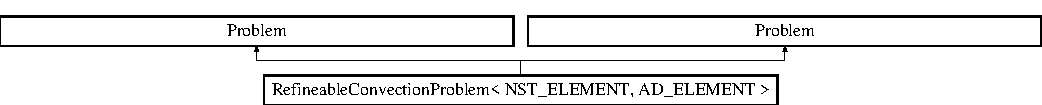
\includegraphics[height=1.417722cm]{classRefineableConvectionProblem}
\end{center}
\end{figure}
\subsection*{Public Member Functions}
\begin{DoxyCompactItemize}
\item 
\hyperlink{classRefineableConvectionProblem_a97e661986093402bf55fb6c32b782ddc}{Refineable\+Convection\+Problem} ()
\begin{DoxyCompactList}\small\item\em Constructor. \end{DoxyCompactList}\item 
\hyperlink{classRefineableConvectionProblem_a43fc2693230601928578d5b0c6380943}{$\sim$\+Refineable\+Convection\+Problem} ()
\begin{DoxyCompactList}\small\item\em Destructor. Empty. \end{DoxyCompactList}\item 
void \hyperlink{classRefineableConvectionProblem_a694f0be87fe09a30d94e92acfce85eee}{actions\+\_\+before\+\_\+newton\+\_\+solve} ()
\begin{DoxyCompactList}\small\item\em Update the problem specs before solve\+: \end{DoxyCompactList}\item 
void \hyperlink{classRefineableConvectionProblem_a13bda5e5e75928efa88433902ccab7ee}{actions\+\_\+after\+\_\+newton\+\_\+solve} ()
\begin{DoxyCompactList}\small\item\em Update the problem after solve (empty) \end{DoxyCompactList}\item 
Refineable\+Rectangular\+Quad\+Mesh$<$ N\+S\+T\+\_\+\+E\+L\+E\+M\+E\+NT $>$ $\ast$ \hyperlink{classRefineableConvectionProblem_a9c84adefabe5a9ba08ed946577a19071}{nst\+\_\+mesh\+\_\+pt} ()
\begin{DoxyCompactList}\small\item\em Access function to the N\+ST mesh. Casts the pointer to the base Mesh object to the actual mesh type. \end{DoxyCompactList}\item 
Refineable\+Rectangular\+Quad\+Mesh$<$ A\+D\+\_\+\+E\+L\+E\+M\+E\+NT $>$ $\ast$ \hyperlink{classRefineableConvectionProblem_a6070d18df944a34ce2af1514c30ebea2}{adv\+\_\+diff\+\_\+mesh\+\_\+pt} ()
\begin{DoxyCompactList}\small\item\em Access function to the AD mesh. Casts the pointer to the base Mesh object to the actual mesh type. \end{DoxyCompactList}\item 
void \hyperlink{classRefineableConvectionProblem_a962499683ada1233e20055e46b15fdb0}{actions\+\_\+before\+\_\+adapt} ()
\begin{DoxyCompactList}\small\item\em Actions before adapt\+:(empty) \end{DoxyCompactList}\item 
void \hyperlink{classRefineableConvectionProblem_a9baa484155212df5ad2137dd5a348def}{actions\+\_\+after\+\_\+adapt} ()
\begin{DoxyCompactList}\small\item\em Actions after adaptation, reset all sources, then re-\/pin a single pressure degree of freedom. \end{DoxyCompactList}\item 
void \hyperlink{classRefineableConvectionProblem_a3432fe8f8e4ba54d5e4c1ca7b3b233e2}{fix\+\_\+pressure} (const unsigned \&e, const unsigned \&pdof, const double \&pvalue)
\begin{DoxyCompactList}\small\item\em Fix pressure in element e at pressure dof pdof and set to pvalue. \end{DoxyCompactList}\item 
void \hyperlink{classRefineableConvectionProblem_aa97926281f88014ad45f43972184a77c}{enable\+\_\+imperfection} ()
\begin{DoxyCompactList}\small\item\em Set the boundary condition on the upper wall to be perturbed slightly to force the solution into the symmetry broken state. \end{DoxyCompactList}\item 
void \hyperlink{classRefineableConvectionProblem_a816f49163ff3ceb71aec4236aac10d84}{disable\+\_\+imperfection} ()
\begin{DoxyCompactList}\small\item\em Set th boundary condition on the upper wall to be unperturbed. \end{DoxyCompactList}\item 
void \hyperlink{classRefineableConvectionProblem_a47efcb3467931e13e12687303135e38b}{doc\+\_\+solution} ()
\begin{DoxyCompactList}\small\item\em Doc the solution. \end{DoxyCompactList}\item 
\hyperlink{classRefineableConvectionProblem_aa3a0c85ea1db9186292d130a3ec23a2d}{Refineable\+Convection\+Problem} ()
\begin{DoxyCompactList}\small\item\em Constructor. \end{DoxyCompactList}\item 
\hyperlink{classRefineableConvectionProblem_a43fc2693230601928578d5b0c6380943}{$\sim$\+Refineable\+Convection\+Problem} ()
\begin{DoxyCompactList}\small\item\em Destructor. Empty. \end{DoxyCompactList}\item 
void \hyperlink{classRefineableConvectionProblem_ae0e627f882cd8faa305392e615331e51}{actions\+\_\+before\+\_\+newton\+\_\+solve} ()
\begin{DoxyCompactList}\small\item\em Update the problem specs before solve\+: \end{DoxyCompactList}\item 
void \hyperlink{classRefineableConvectionProblem_a13bda5e5e75928efa88433902ccab7ee}{actions\+\_\+after\+\_\+newton\+\_\+solve} ()
\begin{DoxyCompactList}\small\item\em Update the problem after solve (empty) \end{DoxyCompactList}\item 
Rectangular\+Quad\+Mesh$<$ E\+L\+E\+M\+E\+NT $>$ $\ast$ \hyperlink{classRefineableConvectionProblem_a837d2412cee6996c78a2d2c5adf720f3}{mesh\+\_\+pt} ()
\begin{DoxyCompactList}\small\item\em Overloaded version of the problem\textquotesingle{}s access function to the mesh. Recasts the pointer to the base Mesh object to the actual mesh type. \end{DoxyCompactList}\item 
void \hyperlink{classRefineableConvectionProblem_a962499683ada1233e20055e46b15fdb0}{actions\+\_\+before\+\_\+adapt} ()
\begin{DoxyCompactList}\small\item\em Actions before adapt\+:(empty) \end{DoxyCompactList}\item 
void \hyperlink{classRefineableConvectionProblem_a9baa484155212df5ad2137dd5a348def}{actions\+\_\+after\+\_\+adapt} ()
\begin{DoxyCompactList}\small\item\em Actions after adaptation, Re-\/pin a single pressure degree of freedom. \end{DoxyCompactList}\item 
void \hyperlink{classRefineableConvectionProblem_a3432fe8f8e4ba54d5e4c1ca7b3b233e2}{fix\+\_\+pressure} (const unsigned \&e, const unsigned \&pdof, const double \&pvalue)
\begin{DoxyCompactList}\small\item\em Fix pressure in element e at pressure dof pdof and set to pvalue. \end{DoxyCompactList}\item 
void \hyperlink{classRefineableConvectionProblem_aa97926281f88014ad45f43972184a77c}{enable\+\_\+imperfection} ()
\begin{DoxyCompactList}\small\item\em Set the boundary condition on the upper wall to be perturbed slightly to force the solution into the symmetry broken state. \end{DoxyCompactList}\item 
void \hyperlink{classRefineableConvectionProblem_a816f49163ff3ceb71aec4236aac10d84}{disable\+\_\+imperfection} ()
\begin{DoxyCompactList}\small\item\em Set the boundary condition on the upper wall to be unperturbed. \end{DoxyCompactList}\item 
void \hyperlink{classRefineableConvectionProblem_a8f6c4ead999c108394b6c6eb121daa51}{doc\+\_\+solution} ()
\begin{DoxyCompactList}\small\item\em Doc the solution. \end{DoxyCompactList}\end{DoxyCompactItemize}
\subsection*{Protected Attributes}
\begin{DoxyCompactItemize}
\item 
Refineable\+Rectangular\+Quad\+Mesh$<$ N\+S\+T\+\_\+\+E\+L\+E\+M\+E\+NT $>$ $\ast$ \hyperlink{classRefineableConvectionProblem_abc03f2233894203f55be5841857d2381}{Nst\+\_\+mesh\+\_\+pt}
\begin{DoxyCompactList}\small\item\em Navier Stokes mesh. \end{DoxyCompactList}\item 
Refineable\+Rectangular\+Quad\+Mesh$<$ A\+D\+\_\+\+E\+L\+E\+M\+E\+NT $>$ $\ast$ \hyperlink{classRefineableConvectionProblem_abfa55603a761cf57cb7de38beb8fa9ac}{Adv\+\_\+diff\+\_\+mesh\+\_\+pt}
\begin{DoxyCompactList}\small\item\em Advection diffusion mesh. \end{DoxyCompactList}\end{DoxyCompactItemize}
\subsection*{Private Attributes}
\begin{DoxyCompactItemize}
\item 
Doc\+Info \hyperlink{classRefineableConvectionProblem_acf0b222e2ae8efc508536e578c3a359e}{Doc\+\_\+info}
\begin{DoxyCompactList}\small\item\em Doc\+Info object. \end{DoxyCompactList}\item 
bool \hyperlink{classRefineableConvectionProblem_af5a23ac1fe5407159089c5909e86f026}{Imperfect}
\begin{DoxyCompactList}\small\item\em Is the boundary condition imperfect or not. \end{DoxyCompactList}\end{DoxyCompactItemize}


\subsection{Detailed Description}
\subsubsection*{template$<$class N\+S\+T\+\_\+\+E\+L\+E\+M\+E\+NT, class A\+D\+\_\+\+E\+L\+E\+M\+E\+NT$>$\newline
class Refineable\+Convection\+Problem$<$ N\+S\+T\+\_\+\+E\+L\+E\+M\+E\+N\+T, A\+D\+\_\+\+E\+L\+E\+M\+E\+N\+T $>$}

2D Convection problem on two rectangular domains, discretised with refineable Navier-\/\+Stokes and Advection-\/\+Diffusion elements. The specific type of element is specified via the template parameters.

2D Convection problem on rectangular domain, discretised with refineable elements. The specific type of element is specified via the template parameter. 

Definition at line 84 of file multi\+\_\+domain\+\_\+ref\+\_\+b\+\_\+convection.\+cc.



\subsection{Constructor \& Destructor Documentation}
\mbox{\Hypertarget{classRefineableConvectionProblem_a97e661986093402bf55fb6c32b782ddc}\label{classRefineableConvectionProblem_a97e661986093402bf55fb6c32b782ddc}} 
\index{Refineable\+Convection\+Problem@{Refineable\+Convection\+Problem}!Refineable\+Convection\+Problem@{Refineable\+Convection\+Problem}}
\index{Refineable\+Convection\+Problem@{Refineable\+Convection\+Problem}!Refineable\+Convection\+Problem@{Refineable\+Convection\+Problem}}
\subsubsection{\texorpdfstring{Refineable\+Convection\+Problem()}{RefineableConvectionProblem()}\hspace{0.1cm}{\footnotesize\ttfamily [1/2]}}
{\footnotesize\ttfamily template$<$class E\+L\+E\+M\+E\+NT $>$ \\
\hyperlink{classRefineableConvectionProblem}{Refineable\+Convection\+Problem}$<$ E\+L\+E\+M\+E\+NT $>$\+::\hyperlink{classRefineableConvectionProblem}{Refineable\+Convection\+Problem} (\begin{DoxyParamCaption}{ }\end{DoxyParamCaption})}



Constructor. 

Constructor for adaptive thermal convection problem. 

Definition at line 191 of file multi\+\_\+domain\+\_\+ref\+\_\+b\+\_\+convection.\+cc.



References Global\+\_\+\+Physical\+\_\+\+Variables\+::\+Direction\+\_\+of\+\_\+gravity(), Global\+\_\+\+Physical\+\_\+\+Variables\+::\+Inverse\+\_\+\+Prandtl, Global\+\_\+\+Physical\+\_\+\+Variables\+::\+Peclet, and Global\+\_\+\+Physical\+\_\+\+Variables\+::\+Rayleigh.



Referenced by Refineable\+Convection\+Problem$<$ N\+S\+T\+\_\+\+E\+L\+E\+M\+E\+N\+T, A\+D\+\_\+\+E\+L\+E\+M\+E\+N\+T $>$\+::disable\+\_\+imperfection().

\mbox{\Hypertarget{classRefineableConvectionProblem_a43fc2693230601928578d5b0c6380943}\label{classRefineableConvectionProblem_a43fc2693230601928578d5b0c6380943}} 
\index{Refineable\+Convection\+Problem@{Refineable\+Convection\+Problem}!````~Refineable\+Convection\+Problem@{$\sim$\+Refineable\+Convection\+Problem}}
\index{````~Refineable\+Convection\+Problem@{$\sim$\+Refineable\+Convection\+Problem}!Refineable\+Convection\+Problem@{Refineable\+Convection\+Problem}}
\subsubsection{\texorpdfstring{$\sim$\+Refineable\+Convection\+Problem()}{~RefineableConvectionProblem()}\hspace{0.1cm}{\footnotesize\ttfamily [1/2]}}
{\footnotesize\ttfamily template$<$class N\+S\+T\+\_\+\+E\+L\+E\+M\+E\+NT , class A\+D\+\_\+\+E\+L\+E\+M\+E\+NT $>$ \\
\hyperlink{classRefineableConvectionProblem}{Refineable\+Convection\+Problem}$<$ N\+S\+T\+\_\+\+E\+L\+E\+M\+E\+NT, A\+D\+\_\+\+E\+L\+E\+M\+E\+NT $>$\+::$\sim$\hyperlink{classRefineableConvectionProblem}{Refineable\+Convection\+Problem} (\begin{DoxyParamCaption}{ }\end{DoxyParamCaption})\hspace{0.3cm}{\ttfamily [inline]}}



Destructor. Empty. 



Definition at line 93 of file multi\+\_\+domain\+\_\+ref\+\_\+b\+\_\+convection.\+cc.

\mbox{\Hypertarget{classRefineableConvectionProblem_aa3a0c85ea1db9186292d130a3ec23a2d}\label{classRefineableConvectionProblem_aa3a0c85ea1db9186292d130a3ec23a2d}} 
\index{Refineable\+Convection\+Problem@{Refineable\+Convection\+Problem}!Refineable\+Convection\+Problem@{Refineable\+Convection\+Problem}}
\index{Refineable\+Convection\+Problem@{Refineable\+Convection\+Problem}!Refineable\+Convection\+Problem@{Refineable\+Convection\+Problem}}
\subsubsection{\texorpdfstring{Refineable\+Convection\+Problem()}{RefineableConvectionProblem()}\hspace{0.1cm}{\footnotesize\ttfamily [2/2]}}
{\footnotesize\ttfamily template$<$class N\+S\+T\+\_\+\+E\+L\+E\+M\+E\+NT , class A\+D\+\_\+\+E\+L\+E\+M\+E\+NT $>$ \\
\hyperlink{classRefineableConvectionProblem}{Refineable\+Convection\+Problem}$<$ N\+S\+T\+\_\+\+E\+L\+E\+M\+E\+NT, A\+D\+\_\+\+E\+L\+E\+M\+E\+NT $>$\+::\hyperlink{classRefineableConvectionProblem}{Refineable\+Convection\+Problem} (\begin{DoxyParamCaption}{ }\end{DoxyParamCaption})}



Constructor. 

\mbox{\Hypertarget{classRefineableConvectionProblem_a43fc2693230601928578d5b0c6380943}\label{classRefineableConvectionProblem_a43fc2693230601928578d5b0c6380943}} 
\index{Refineable\+Convection\+Problem@{Refineable\+Convection\+Problem}!````~Refineable\+Convection\+Problem@{$\sim$\+Refineable\+Convection\+Problem}}
\index{````~Refineable\+Convection\+Problem@{$\sim$\+Refineable\+Convection\+Problem}!Refineable\+Convection\+Problem@{Refineable\+Convection\+Problem}}
\subsubsection{\texorpdfstring{$\sim$\+Refineable\+Convection\+Problem()}{~RefineableConvectionProblem()}\hspace{0.1cm}{\footnotesize\ttfamily [2/2]}}
{\footnotesize\ttfamily template$<$class N\+S\+T\+\_\+\+E\+L\+E\+M\+E\+NT , class A\+D\+\_\+\+E\+L\+E\+M\+E\+NT $>$ \\
\hyperlink{classRefineableConvectionProblem}{Refineable\+Convection\+Problem}$<$ N\+S\+T\+\_\+\+E\+L\+E\+M\+E\+NT, A\+D\+\_\+\+E\+L\+E\+M\+E\+NT $>$\+::$\sim$\hyperlink{classRefineableConvectionProblem}{Refineable\+Convection\+Problem} (\begin{DoxyParamCaption}{ }\end{DoxyParamCaption})\hspace{0.3cm}{\ttfamily [inline]}}



Destructor. Empty. 



Definition at line 97 of file refineable\+\_\+b\+\_\+convection.\+cc.



\subsection{Member Function Documentation}
\mbox{\Hypertarget{classRefineableConvectionProblem_a9baa484155212df5ad2137dd5a348def}\label{classRefineableConvectionProblem_a9baa484155212df5ad2137dd5a348def}} 
\index{Refineable\+Convection\+Problem@{Refineable\+Convection\+Problem}!actions\+\_\+after\+\_\+adapt@{actions\+\_\+after\+\_\+adapt}}
\index{actions\+\_\+after\+\_\+adapt@{actions\+\_\+after\+\_\+adapt}!Refineable\+Convection\+Problem@{Refineable\+Convection\+Problem}}
\subsubsection{\texorpdfstring{actions\+\_\+after\+\_\+adapt()}{actions\_after\_adapt()}\hspace{0.1cm}{\footnotesize\ttfamily [1/2]}}
{\footnotesize\ttfamily template$<$class N\+S\+T\+\_\+\+E\+L\+E\+M\+E\+NT , class A\+D\+\_\+\+E\+L\+E\+M\+E\+NT $>$ \\
void \hyperlink{classRefineableConvectionProblem}{Refineable\+Convection\+Problem}$<$ N\+S\+T\+\_\+\+E\+L\+E\+M\+E\+NT, A\+D\+\_\+\+E\+L\+E\+M\+E\+NT $>$\+::actions\+\_\+after\+\_\+adapt (\begin{DoxyParamCaption}{ }\end{DoxyParamCaption})\hspace{0.3cm}{\ttfamily [inline]}}



Actions after adaptation, Re-\/pin a single pressure degree of freedom. 



Definition at line 119 of file refineable\+\_\+b\+\_\+convection.\+cc.

\mbox{\Hypertarget{classRefineableConvectionProblem_a9baa484155212df5ad2137dd5a348def}\label{classRefineableConvectionProblem_a9baa484155212df5ad2137dd5a348def}} 
\index{Refineable\+Convection\+Problem@{Refineable\+Convection\+Problem}!actions\+\_\+after\+\_\+adapt@{actions\+\_\+after\+\_\+adapt}}
\index{actions\+\_\+after\+\_\+adapt@{actions\+\_\+after\+\_\+adapt}!Refineable\+Convection\+Problem@{Refineable\+Convection\+Problem}}
\subsubsection{\texorpdfstring{actions\+\_\+after\+\_\+adapt()}{actions\_after\_adapt()}\hspace{0.1cm}{\footnotesize\ttfamily [2/2]}}
{\footnotesize\ttfamily template$<$class N\+S\+T\+\_\+\+E\+L\+E\+M\+E\+NT , class A\+D\+\_\+\+E\+L\+E\+M\+E\+NT $>$ \\
void \hyperlink{classRefineableConvectionProblem}{Refineable\+Convection\+Problem}$<$ N\+S\+T\+\_\+\+E\+L\+E\+M\+E\+NT, A\+D\+\_\+\+E\+L\+E\+M\+E\+NT $>$\+::actions\+\_\+after\+\_\+adapt (\begin{DoxyParamCaption}{ }\end{DoxyParamCaption})\hspace{0.3cm}{\ttfamily [inline]}}



Actions after adaptation, reset all sources, then re-\/pin a single pressure degree of freedom. 



Definition at line 124 of file multi\+\_\+domain\+\_\+ref\+\_\+b\+\_\+convection.\+cc.

\mbox{\Hypertarget{classRefineableConvectionProblem_a13bda5e5e75928efa88433902ccab7ee}\label{classRefineableConvectionProblem_a13bda5e5e75928efa88433902ccab7ee}} 
\index{Refineable\+Convection\+Problem@{Refineable\+Convection\+Problem}!actions\+\_\+after\+\_\+newton\+\_\+solve@{actions\+\_\+after\+\_\+newton\+\_\+solve}}
\index{actions\+\_\+after\+\_\+newton\+\_\+solve@{actions\+\_\+after\+\_\+newton\+\_\+solve}!Refineable\+Convection\+Problem@{Refineable\+Convection\+Problem}}
\subsubsection{\texorpdfstring{actions\+\_\+after\+\_\+newton\+\_\+solve()}{actions\_after\_newton\_solve()}\hspace{0.1cm}{\footnotesize\ttfamily [1/2]}}
{\footnotesize\ttfamily template$<$class N\+S\+T\+\_\+\+E\+L\+E\+M\+E\+NT , class A\+D\+\_\+\+E\+L\+E\+M\+E\+NT $>$ \\
void \hyperlink{classRefineableConvectionProblem}{Refineable\+Convection\+Problem}$<$ N\+S\+T\+\_\+\+E\+L\+E\+M\+E\+NT, A\+D\+\_\+\+E\+L\+E\+M\+E\+NT $>$\+::actions\+\_\+after\+\_\+newton\+\_\+solve (\begin{DoxyParamCaption}{ }\end{DoxyParamCaption})\hspace{0.3cm}{\ttfamily [inline]}}



Update the problem after solve (empty) 



Definition at line 99 of file multi\+\_\+domain\+\_\+ref\+\_\+b\+\_\+convection.\+cc.

\mbox{\Hypertarget{classRefineableConvectionProblem_a13bda5e5e75928efa88433902ccab7ee}\label{classRefineableConvectionProblem_a13bda5e5e75928efa88433902ccab7ee}} 
\index{Refineable\+Convection\+Problem@{Refineable\+Convection\+Problem}!actions\+\_\+after\+\_\+newton\+\_\+solve@{actions\+\_\+after\+\_\+newton\+\_\+solve}}
\index{actions\+\_\+after\+\_\+newton\+\_\+solve@{actions\+\_\+after\+\_\+newton\+\_\+solve}!Refineable\+Convection\+Problem@{Refineable\+Convection\+Problem}}
\subsubsection{\texorpdfstring{actions\+\_\+after\+\_\+newton\+\_\+solve()}{actions\_after\_newton\_solve()}\hspace{0.1cm}{\footnotesize\ttfamily [2/2]}}
{\footnotesize\ttfamily template$<$class N\+S\+T\+\_\+\+E\+L\+E\+M\+E\+NT , class A\+D\+\_\+\+E\+L\+E\+M\+E\+NT $>$ \\
void \hyperlink{classRefineableConvectionProblem}{Refineable\+Convection\+Problem}$<$ N\+S\+T\+\_\+\+E\+L\+E\+M\+E\+NT, A\+D\+\_\+\+E\+L\+E\+M\+E\+NT $>$\+::actions\+\_\+after\+\_\+newton\+\_\+solve (\begin{DoxyParamCaption}{ }\end{DoxyParamCaption})\hspace{0.3cm}{\ttfamily [inline]}}



Update the problem after solve (empty) 



Definition at line 103 of file refineable\+\_\+b\+\_\+convection.\+cc.

\mbox{\Hypertarget{classRefineableConvectionProblem_a962499683ada1233e20055e46b15fdb0}\label{classRefineableConvectionProblem_a962499683ada1233e20055e46b15fdb0}} 
\index{Refineable\+Convection\+Problem@{Refineable\+Convection\+Problem}!actions\+\_\+before\+\_\+adapt@{actions\+\_\+before\+\_\+adapt}}
\index{actions\+\_\+before\+\_\+adapt@{actions\+\_\+before\+\_\+adapt}!Refineable\+Convection\+Problem@{Refineable\+Convection\+Problem}}
\subsubsection{\texorpdfstring{actions\+\_\+before\+\_\+adapt()}{actions\_before\_adapt()}\hspace{0.1cm}{\footnotesize\ttfamily [1/2]}}
{\footnotesize\ttfamily template$<$class N\+S\+T\+\_\+\+E\+L\+E\+M\+E\+NT , class A\+D\+\_\+\+E\+L\+E\+M\+E\+NT $>$ \\
void \hyperlink{classRefineableConvectionProblem}{Refineable\+Convection\+Problem}$<$ N\+S\+T\+\_\+\+E\+L\+E\+M\+E\+NT, A\+D\+\_\+\+E\+L\+E\+M\+E\+NT $>$\+::actions\+\_\+before\+\_\+adapt (\begin{DoxyParamCaption}{ }\end{DoxyParamCaption})\hspace{0.3cm}{\ttfamily [inline]}}



Actions before adapt\+:(empty) 



Definition at line 115 of file refineable\+\_\+b\+\_\+convection.\+cc.

\mbox{\Hypertarget{classRefineableConvectionProblem_a962499683ada1233e20055e46b15fdb0}\label{classRefineableConvectionProblem_a962499683ada1233e20055e46b15fdb0}} 
\index{Refineable\+Convection\+Problem@{Refineable\+Convection\+Problem}!actions\+\_\+before\+\_\+adapt@{actions\+\_\+before\+\_\+adapt}}
\index{actions\+\_\+before\+\_\+adapt@{actions\+\_\+before\+\_\+adapt}!Refineable\+Convection\+Problem@{Refineable\+Convection\+Problem}}
\subsubsection{\texorpdfstring{actions\+\_\+before\+\_\+adapt()}{actions\_before\_adapt()}\hspace{0.1cm}{\footnotesize\ttfamily [2/2]}}
{\footnotesize\ttfamily template$<$class N\+S\+T\+\_\+\+E\+L\+E\+M\+E\+NT , class A\+D\+\_\+\+E\+L\+E\+M\+E\+NT $>$ \\
void \hyperlink{classRefineableConvectionProblem}{Refineable\+Convection\+Problem}$<$ N\+S\+T\+\_\+\+E\+L\+E\+M\+E\+NT, A\+D\+\_\+\+E\+L\+E\+M\+E\+NT $>$\+::actions\+\_\+before\+\_\+adapt (\begin{DoxyParamCaption}{ }\end{DoxyParamCaption})\hspace{0.3cm}{\ttfamily [inline]}}



Actions before adapt\+:(empty) 



Definition at line 120 of file multi\+\_\+domain\+\_\+ref\+\_\+b\+\_\+convection.\+cc.

\mbox{\Hypertarget{classRefineableConvectionProblem_a694f0be87fe09a30d94e92acfce85eee}\label{classRefineableConvectionProblem_a694f0be87fe09a30d94e92acfce85eee}} 
\index{Refineable\+Convection\+Problem@{Refineable\+Convection\+Problem}!actions\+\_\+before\+\_\+newton\+\_\+solve@{actions\+\_\+before\+\_\+newton\+\_\+solve}}
\index{actions\+\_\+before\+\_\+newton\+\_\+solve@{actions\+\_\+before\+\_\+newton\+\_\+solve}!Refineable\+Convection\+Problem@{Refineable\+Convection\+Problem}}
\subsubsection{\texorpdfstring{actions\+\_\+before\+\_\+newton\+\_\+solve()}{actions\_before\_newton\_solve()}\hspace{0.1cm}{\footnotesize\ttfamily [1/2]}}
{\footnotesize\ttfamily template$<$class E\+L\+E\+M\+E\+NT $>$ \\
void \hyperlink{classRefineableConvectionProblem}{Refineable\+Convection\+Problem}$<$ E\+L\+E\+M\+E\+NT $>$\+::actions\+\_\+before\+\_\+newton\+\_\+solve (\begin{DoxyParamCaption}{ }\end{DoxyParamCaption})}



Update the problem specs before solve\+: 

Update the problem specs before solve\+: (Re-\/)set boundary conditions to include an imperfection (or not) depending on the control flag. 

Definition at line 368 of file multi\+\_\+domain\+\_\+ref\+\_\+b\+\_\+convection.\+cc.



Referenced by Refineable\+Convection\+Problem$<$ N\+S\+T\+\_\+\+E\+L\+E\+M\+E\+N\+T, A\+D\+\_\+\+E\+L\+E\+M\+E\+N\+T $>$\+::disable\+\_\+imperfection().

\mbox{\Hypertarget{classRefineableConvectionProblem_ae0e627f882cd8faa305392e615331e51}\label{classRefineableConvectionProblem_ae0e627f882cd8faa305392e615331e51}} 
\index{Refineable\+Convection\+Problem@{Refineable\+Convection\+Problem}!actions\+\_\+before\+\_\+newton\+\_\+solve@{actions\+\_\+before\+\_\+newton\+\_\+solve}}
\index{actions\+\_\+before\+\_\+newton\+\_\+solve@{actions\+\_\+before\+\_\+newton\+\_\+solve}!Refineable\+Convection\+Problem@{Refineable\+Convection\+Problem}}
\subsubsection{\texorpdfstring{actions\+\_\+before\+\_\+newton\+\_\+solve()}{actions\_before\_newton\_solve()}\hspace{0.1cm}{\footnotesize\ttfamily [2/2]}}
{\footnotesize\ttfamily template$<$class N\+S\+T\+\_\+\+E\+L\+E\+M\+E\+NT , class A\+D\+\_\+\+E\+L\+E\+M\+E\+NT $>$ \\
void \hyperlink{classRefineableConvectionProblem}{Refineable\+Convection\+Problem}$<$ N\+S\+T\+\_\+\+E\+L\+E\+M\+E\+NT, A\+D\+\_\+\+E\+L\+E\+M\+E\+NT $>$\+::actions\+\_\+before\+\_\+newton\+\_\+solve (\begin{DoxyParamCaption}{ }\end{DoxyParamCaption})}



Update the problem specs before solve\+: 

\mbox{\Hypertarget{classRefineableConvectionProblem_a6070d18df944a34ce2af1514c30ebea2}\label{classRefineableConvectionProblem_a6070d18df944a34ce2af1514c30ebea2}} 
\index{Refineable\+Convection\+Problem@{Refineable\+Convection\+Problem}!adv\+\_\+diff\+\_\+mesh\+\_\+pt@{adv\+\_\+diff\+\_\+mesh\+\_\+pt}}
\index{adv\+\_\+diff\+\_\+mesh\+\_\+pt@{adv\+\_\+diff\+\_\+mesh\+\_\+pt}!Refineable\+Convection\+Problem@{Refineable\+Convection\+Problem}}
\subsubsection{\texorpdfstring{adv\+\_\+diff\+\_\+mesh\+\_\+pt()}{adv\_diff\_mesh\_pt()}}
{\footnotesize\ttfamily template$<$class N\+S\+T\+\_\+\+E\+L\+E\+M\+E\+NT , class A\+D\+\_\+\+E\+L\+E\+M\+E\+NT $>$ \\
Refineable\+Rectangular\+Quad\+Mesh$<$A\+D\+\_\+\+E\+L\+E\+M\+E\+NT$>$$\ast$ \hyperlink{classRefineableConvectionProblem}{Refineable\+Convection\+Problem}$<$ N\+S\+T\+\_\+\+E\+L\+E\+M\+E\+NT, A\+D\+\_\+\+E\+L\+E\+M\+E\+NT $>$\+::adv\+\_\+diff\+\_\+mesh\+\_\+pt (\begin{DoxyParamCaption}{ }\end{DoxyParamCaption})\hspace{0.3cm}{\ttfamily [inline]}}



Access function to the AD mesh. Casts the pointer to the base Mesh object to the actual mesh type. 



Definition at line 113 of file multi\+\_\+domain\+\_\+ref\+\_\+b\+\_\+convection.\+cc.

\mbox{\Hypertarget{classRefineableConvectionProblem_a816f49163ff3ceb71aec4236aac10d84}\label{classRefineableConvectionProblem_a816f49163ff3ceb71aec4236aac10d84}} 
\index{Refineable\+Convection\+Problem@{Refineable\+Convection\+Problem}!disable\+\_\+imperfection@{disable\+\_\+imperfection}}
\index{disable\+\_\+imperfection@{disable\+\_\+imperfection}!Refineable\+Convection\+Problem@{Refineable\+Convection\+Problem}}
\subsubsection{\texorpdfstring{disable\+\_\+imperfection()}{disable\_imperfection()}\hspace{0.1cm}{\footnotesize\ttfamily [1/2]}}
{\footnotesize\ttfamily template$<$class N\+S\+T\+\_\+\+E\+L\+E\+M\+E\+NT , class A\+D\+\_\+\+E\+L\+E\+M\+E\+NT $>$ \\
void \hyperlink{classRefineableConvectionProblem}{Refineable\+Convection\+Problem}$<$ N\+S\+T\+\_\+\+E\+L\+E\+M\+E\+NT, A\+D\+\_\+\+E\+L\+E\+M\+E\+NT $>$\+::disable\+\_\+imperfection (\begin{DoxyParamCaption}{ }\end{DoxyParamCaption})\hspace{0.3cm}{\ttfamily [inline]}}



Set the boundary condition on the upper wall to be unperturbed. 



Definition at line 146 of file refineable\+\_\+b\+\_\+convection.\+cc.



References Refineable\+Convection\+Problem$<$ N\+S\+T\+\_\+\+E\+L\+E\+M\+E\+N\+T, A\+D\+\_\+\+E\+L\+E\+M\+E\+N\+T $>$\+::actions\+\_\+before\+\_\+newton\+\_\+solve(), Global\+\_\+\+Physical\+\_\+\+Variables\+::\+Direction\+\_\+of\+\_\+gravity(), Refineable\+Convection\+Problem$<$ N\+S\+T\+\_\+\+E\+L\+E\+M\+E\+N\+T, A\+D\+\_\+\+E\+L\+E\+M\+E\+N\+T $>$\+::doc\+\_\+solution(), Global\+\_\+\+Physical\+\_\+\+Variables\+::\+Inverse\+\_\+\+Prandtl, Global\+\_\+\+Physical\+\_\+\+Variables\+::\+Peclet, Global\+\_\+\+Physical\+\_\+\+Variables\+::\+Rayleigh, and Refineable\+Convection\+Problem$<$ N\+S\+T\+\_\+\+E\+L\+E\+M\+E\+N\+T, A\+D\+\_\+\+E\+L\+E\+M\+E\+N\+T $>$\+::\+Refineable\+Convection\+Problem().

\mbox{\Hypertarget{classRefineableConvectionProblem_a816f49163ff3ceb71aec4236aac10d84}\label{classRefineableConvectionProblem_a816f49163ff3ceb71aec4236aac10d84}} 
\index{Refineable\+Convection\+Problem@{Refineable\+Convection\+Problem}!disable\+\_\+imperfection@{disable\+\_\+imperfection}}
\index{disable\+\_\+imperfection@{disable\+\_\+imperfection}!Refineable\+Convection\+Problem@{Refineable\+Convection\+Problem}}
\subsubsection{\texorpdfstring{disable\+\_\+imperfection()}{disable\_imperfection()}\hspace{0.1cm}{\footnotesize\ttfamily [2/2]}}
{\footnotesize\ttfamily template$<$class N\+S\+T\+\_\+\+E\+L\+E\+M\+E\+NT , class A\+D\+\_\+\+E\+L\+E\+M\+E\+NT $>$ \\
void \hyperlink{classRefineableConvectionProblem}{Refineable\+Convection\+Problem}$<$ N\+S\+T\+\_\+\+E\+L\+E\+M\+E\+NT, A\+D\+\_\+\+E\+L\+E\+M\+E\+NT $>$\+::disable\+\_\+imperfection (\begin{DoxyParamCaption}{ }\end{DoxyParamCaption})\hspace{0.3cm}{\ttfamily [inline]}}



Set th boundary condition on the upper wall to be unperturbed. 



Definition at line 162 of file multi\+\_\+domain\+\_\+ref\+\_\+b\+\_\+convection.\+cc.

\mbox{\Hypertarget{classRefineableConvectionProblem_a8f6c4ead999c108394b6c6eb121daa51}\label{classRefineableConvectionProblem_a8f6c4ead999c108394b6c6eb121daa51}} 
\index{Refineable\+Convection\+Problem@{Refineable\+Convection\+Problem}!doc\+\_\+solution@{doc\+\_\+solution}}
\index{doc\+\_\+solution@{doc\+\_\+solution}!Refineable\+Convection\+Problem@{Refineable\+Convection\+Problem}}
\subsubsection{\texorpdfstring{doc\+\_\+solution()}{doc\_solution()}\hspace{0.1cm}{\footnotesize\ttfamily [1/2]}}
{\footnotesize\ttfamily template$<$class N\+S\+T\+\_\+\+E\+L\+E\+M\+E\+NT , class A\+D\+\_\+\+E\+L\+E\+M\+E\+NT $>$ \\
void \hyperlink{classRefineableConvectionProblem}{Refineable\+Convection\+Problem}$<$ N\+S\+T\+\_\+\+E\+L\+E\+M\+E\+NT, A\+D\+\_\+\+E\+L\+E\+M\+E\+NT $>$\+::doc\+\_\+solution (\begin{DoxyParamCaption}{ }\end{DoxyParamCaption})}



Doc the solution. 

\mbox{\Hypertarget{classRefineableConvectionProblem_a47efcb3467931e13e12687303135e38b}\label{classRefineableConvectionProblem_a47efcb3467931e13e12687303135e38b}} 
\index{Refineable\+Convection\+Problem@{Refineable\+Convection\+Problem}!doc\+\_\+solution@{doc\+\_\+solution}}
\index{doc\+\_\+solution@{doc\+\_\+solution}!Refineable\+Convection\+Problem@{Refineable\+Convection\+Problem}}
\subsubsection{\texorpdfstring{doc\+\_\+solution()}{doc\_solution()}\hspace{0.1cm}{\footnotesize\ttfamily [2/2]}}
{\footnotesize\ttfamily template$<$class E\+L\+E\+M\+E\+NT $>$ \\
void \hyperlink{classRefineableConvectionProblem}{Refineable\+Convection\+Problem}$<$ E\+L\+E\+M\+E\+NT $>$\+::doc\+\_\+solution (\begin{DoxyParamCaption}{ }\end{DoxyParamCaption})}



Doc the solution. 



Definition at line 436 of file multi\+\_\+domain\+\_\+ref\+\_\+b\+\_\+convection.\+cc.



Referenced by Refineable\+Convection\+Problem$<$ N\+S\+T\+\_\+\+E\+L\+E\+M\+E\+N\+T, A\+D\+\_\+\+E\+L\+E\+M\+E\+N\+T $>$\+::disable\+\_\+imperfection().

\mbox{\Hypertarget{classRefineableConvectionProblem_aa97926281f88014ad45f43972184a77c}\label{classRefineableConvectionProblem_aa97926281f88014ad45f43972184a77c}} 
\index{Refineable\+Convection\+Problem@{Refineable\+Convection\+Problem}!enable\+\_\+imperfection@{enable\+\_\+imperfection}}
\index{enable\+\_\+imperfection@{enable\+\_\+imperfection}!Refineable\+Convection\+Problem@{Refineable\+Convection\+Problem}}
\subsubsection{\texorpdfstring{enable\+\_\+imperfection()}{enable\_imperfection()}\hspace{0.1cm}{\footnotesize\ttfamily [1/2]}}
{\footnotesize\ttfamily template$<$class N\+S\+T\+\_\+\+E\+L\+E\+M\+E\+NT , class A\+D\+\_\+\+E\+L\+E\+M\+E\+NT $>$ \\
void \hyperlink{classRefineableConvectionProblem}{Refineable\+Convection\+Problem}$<$ N\+S\+T\+\_\+\+E\+L\+E\+M\+E\+NT, A\+D\+\_\+\+E\+L\+E\+M\+E\+NT $>$\+::enable\+\_\+imperfection (\begin{DoxyParamCaption}{ }\end{DoxyParamCaption})\hspace{0.3cm}{\ttfamily [inline]}}



Set the boundary condition on the upper wall to be perturbed slightly to force the solution into the symmetry broken state. 



Definition at line 142 of file refineable\+\_\+b\+\_\+convection.\+cc.

\mbox{\Hypertarget{classRefineableConvectionProblem_aa97926281f88014ad45f43972184a77c}\label{classRefineableConvectionProblem_aa97926281f88014ad45f43972184a77c}} 
\index{Refineable\+Convection\+Problem@{Refineable\+Convection\+Problem}!enable\+\_\+imperfection@{enable\+\_\+imperfection}}
\index{enable\+\_\+imperfection@{enable\+\_\+imperfection}!Refineable\+Convection\+Problem@{Refineable\+Convection\+Problem}}
\subsubsection{\texorpdfstring{enable\+\_\+imperfection()}{enable\_imperfection()}\hspace{0.1cm}{\footnotesize\ttfamily [2/2]}}
{\footnotesize\ttfamily template$<$class N\+S\+T\+\_\+\+E\+L\+E\+M\+E\+NT , class A\+D\+\_\+\+E\+L\+E\+M\+E\+NT $>$ \\
void \hyperlink{classRefineableConvectionProblem}{Refineable\+Convection\+Problem}$<$ N\+S\+T\+\_\+\+E\+L\+E\+M\+E\+NT, A\+D\+\_\+\+E\+L\+E\+M\+E\+NT $>$\+::enable\+\_\+imperfection (\begin{DoxyParamCaption}{ }\end{DoxyParamCaption})\hspace{0.3cm}{\ttfamily [inline]}}



Set the boundary condition on the upper wall to be perturbed slightly to force the solution into the symmetry broken state. 



Definition at line 158 of file multi\+\_\+domain\+\_\+ref\+\_\+b\+\_\+convection.\+cc.

\mbox{\Hypertarget{classRefineableConvectionProblem_a3432fe8f8e4ba54d5e4c1ca7b3b233e2}\label{classRefineableConvectionProblem_a3432fe8f8e4ba54d5e4c1ca7b3b233e2}} 
\index{Refineable\+Convection\+Problem@{Refineable\+Convection\+Problem}!fix\+\_\+pressure@{fix\+\_\+pressure}}
\index{fix\+\_\+pressure@{fix\+\_\+pressure}!Refineable\+Convection\+Problem@{Refineable\+Convection\+Problem}}
\subsubsection{\texorpdfstring{fix\+\_\+pressure()}{fix\_pressure()}\hspace{0.1cm}{\footnotesize\ttfamily [1/2]}}
{\footnotesize\ttfamily template$<$class N\+S\+T\+\_\+\+E\+L\+E\+M\+E\+NT , class A\+D\+\_\+\+E\+L\+E\+M\+E\+NT $>$ \\
void \hyperlink{classRefineableConvectionProblem}{Refineable\+Convection\+Problem}$<$ N\+S\+T\+\_\+\+E\+L\+E\+M\+E\+NT, A\+D\+\_\+\+E\+L\+E\+M\+E\+NT $>$\+::fix\+\_\+pressure (\begin{DoxyParamCaption}\item[{const unsigned \&}]{e,  }\item[{const unsigned \&}]{pdof,  }\item[{const double \&}]{pvalue }\end{DoxyParamCaption})\hspace{0.3cm}{\ttfamily [inline]}}



Fix pressure in element e at pressure dof pdof and set to pvalue. 



Definition at line 131 of file refineable\+\_\+b\+\_\+convection.\+cc.

\mbox{\Hypertarget{classRefineableConvectionProblem_a3432fe8f8e4ba54d5e4c1ca7b3b233e2}\label{classRefineableConvectionProblem_a3432fe8f8e4ba54d5e4c1ca7b3b233e2}} 
\index{Refineable\+Convection\+Problem@{Refineable\+Convection\+Problem}!fix\+\_\+pressure@{fix\+\_\+pressure}}
\index{fix\+\_\+pressure@{fix\+\_\+pressure}!Refineable\+Convection\+Problem@{Refineable\+Convection\+Problem}}
\subsubsection{\texorpdfstring{fix\+\_\+pressure()}{fix\_pressure()}\hspace{0.1cm}{\footnotesize\ttfamily [2/2]}}
{\footnotesize\ttfamily template$<$class N\+S\+T\+\_\+\+E\+L\+E\+M\+E\+NT , class A\+D\+\_\+\+E\+L\+E\+M\+E\+NT $>$ \\
void \hyperlink{classRefineableConvectionProblem}{Refineable\+Convection\+Problem}$<$ N\+S\+T\+\_\+\+E\+L\+E\+M\+E\+NT, A\+D\+\_\+\+E\+L\+E\+M\+E\+NT $>$\+::fix\+\_\+pressure (\begin{DoxyParamCaption}\item[{const unsigned \&}]{e,  }\item[{const unsigned \&}]{pdof,  }\item[{const double \&}]{pvalue }\end{DoxyParamCaption})\hspace{0.3cm}{\ttfamily [inline]}}



Fix pressure in element e at pressure dof pdof and set to pvalue. 



Definition at line 143 of file multi\+\_\+domain\+\_\+ref\+\_\+b\+\_\+convection.\+cc.

\mbox{\Hypertarget{classRefineableConvectionProblem_a837d2412cee6996c78a2d2c5adf720f3}\label{classRefineableConvectionProblem_a837d2412cee6996c78a2d2c5adf720f3}} 
\index{Refineable\+Convection\+Problem@{Refineable\+Convection\+Problem}!mesh\+\_\+pt@{mesh\+\_\+pt}}
\index{mesh\+\_\+pt@{mesh\+\_\+pt}!Refineable\+Convection\+Problem@{Refineable\+Convection\+Problem}}
\subsubsection{\texorpdfstring{mesh\+\_\+pt()}{mesh\_pt()}}
{\footnotesize\ttfamily template$<$class N\+S\+T\+\_\+\+E\+L\+E\+M\+E\+NT , class A\+D\+\_\+\+E\+L\+E\+M\+E\+NT $>$ \\
Rectangular\+Quad\+Mesh$<$E\+L\+E\+M\+E\+NT$>$$\ast$ \hyperlink{classRefineableConvectionProblem}{Refineable\+Convection\+Problem}$<$ N\+S\+T\+\_\+\+E\+L\+E\+M\+E\+NT, A\+D\+\_\+\+E\+L\+E\+M\+E\+NT $>$\+::mesh\+\_\+pt (\begin{DoxyParamCaption}{ }\end{DoxyParamCaption})\hspace{0.3cm}{\ttfamily [inline]}}



Overloaded version of the problem\textquotesingle{}s access function to the mesh. Recasts the pointer to the base Mesh object to the actual mesh type. 



Definition at line 108 of file refineable\+\_\+b\+\_\+convection.\+cc.

\mbox{\Hypertarget{classRefineableConvectionProblem_a9c84adefabe5a9ba08ed946577a19071}\label{classRefineableConvectionProblem_a9c84adefabe5a9ba08ed946577a19071}} 
\index{Refineable\+Convection\+Problem@{Refineable\+Convection\+Problem}!nst\+\_\+mesh\+\_\+pt@{nst\+\_\+mesh\+\_\+pt}}
\index{nst\+\_\+mesh\+\_\+pt@{nst\+\_\+mesh\+\_\+pt}!Refineable\+Convection\+Problem@{Refineable\+Convection\+Problem}}
\subsubsection{\texorpdfstring{nst\+\_\+mesh\+\_\+pt()}{nst\_mesh\_pt()}}
{\footnotesize\ttfamily template$<$class N\+S\+T\+\_\+\+E\+L\+E\+M\+E\+NT , class A\+D\+\_\+\+E\+L\+E\+M\+E\+NT $>$ \\
Refineable\+Rectangular\+Quad\+Mesh$<$N\+S\+T\+\_\+\+E\+L\+E\+M\+E\+NT$>$$\ast$ \hyperlink{classRefineableConvectionProblem}{Refineable\+Convection\+Problem}$<$ N\+S\+T\+\_\+\+E\+L\+E\+M\+E\+NT, A\+D\+\_\+\+E\+L\+E\+M\+E\+NT $>$\+::nst\+\_\+mesh\+\_\+pt (\begin{DoxyParamCaption}{ }\end{DoxyParamCaption})\hspace{0.3cm}{\ttfamily [inline]}}



Access function to the N\+ST mesh. Casts the pointer to the base Mesh object to the actual mesh type. 



Definition at line 104 of file multi\+\_\+domain\+\_\+ref\+\_\+b\+\_\+convection.\+cc.



\subsection{Member Data Documentation}
\mbox{\Hypertarget{classRefineableConvectionProblem_abfa55603a761cf57cb7de38beb8fa9ac}\label{classRefineableConvectionProblem_abfa55603a761cf57cb7de38beb8fa9ac}} 
\index{Refineable\+Convection\+Problem@{Refineable\+Convection\+Problem}!Adv\+\_\+diff\+\_\+mesh\+\_\+pt@{Adv\+\_\+diff\+\_\+mesh\+\_\+pt}}
\index{Adv\+\_\+diff\+\_\+mesh\+\_\+pt@{Adv\+\_\+diff\+\_\+mesh\+\_\+pt}!Refineable\+Convection\+Problem@{Refineable\+Convection\+Problem}}
\subsubsection{\texorpdfstring{Adv\+\_\+diff\+\_\+mesh\+\_\+pt}{Adv\_diff\_mesh\_pt}}
{\footnotesize\ttfamily template$<$class N\+S\+T\+\_\+\+E\+L\+E\+M\+E\+NT , class A\+D\+\_\+\+E\+L\+E\+M\+E\+NT $>$ \\
Refineable\+Rectangular\+Quad\+Mesh$<$A\+D\+\_\+\+E\+L\+E\+M\+E\+NT$>$$\ast$ \hyperlink{classRefineableConvectionProblem}{Refineable\+Convection\+Problem}$<$ N\+S\+T\+\_\+\+E\+L\+E\+M\+E\+NT, A\+D\+\_\+\+E\+L\+E\+M\+E\+NT $>$\+::Adv\+\_\+diff\+\_\+mesh\+\_\+pt\hspace{0.3cm}{\ttfamily [protected]}}



Advection diffusion mesh. 



Definition at line 181 of file multi\+\_\+domain\+\_\+ref\+\_\+b\+\_\+convection.\+cc.

\mbox{\Hypertarget{classRefineableConvectionProblem_acf0b222e2ae8efc508536e578c3a359e}\label{classRefineableConvectionProblem_acf0b222e2ae8efc508536e578c3a359e}} 
\index{Refineable\+Convection\+Problem@{Refineable\+Convection\+Problem}!Doc\+\_\+info@{Doc\+\_\+info}}
\index{Doc\+\_\+info@{Doc\+\_\+info}!Refineable\+Convection\+Problem@{Refineable\+Convection\+Problem}}
\subsubsection{\texorpdfstring{Doc\+\_\+info}{Doc\_info}}
{\footnotesize\ttfamily template$<$class N\+S\+T\+\_\+\+E\+L\+E\+M\+E\+NT , class A\+D\+\_\+\+E\+L\+E\+M\+E\+NT $>$ \\
Doc\+Info \hyperlink{classRefineableConvectionProblem}{Refineable\+Convection\+Problem}$<$ N\+S\+T\+\_\+\+E\+L\+E\+M\+E\+NT, A\+D\+\_\+\+E\+L\+E\+M\+E\+NT $>$\+::Doc\+\_\+info\hspace{0.3cm}{\ttfamily [private]}}



Doc\+Info object. 



Definition at line 170 of file multi\+\_\+domain\+\_\+ref\+\_\+b\+\_\+convection.\+cc.

\mbox{\Hypertarget{classRefineableConvectionProblem_af5a23ac1fe5407159089c5909e86f026}\label{classRefineableConvectionProblem_af5a23ac1fe5407159089c5909e86f026}} 
\index{Refineable\+Convection\+Problem@{Refineable\+Convection\+Problem}!Imperfect@{Imperfect}}
\index{Imperfect@{Imperfect}!Refineable\+Convection\+Problem@{Refineable\+Convection\+Problem}}
\subsubsection{\texorpdfstring{Imperfect}{Imperfect}}
{\footnotesize\ttfamily template$<$class N\+S\+T\+\_\+\+E\+L\+E\+M\+E\+NT , class A\+D\+\_\+\+E\+L\+E\+M\+E\+NT $>$ \\
bool \hyperlink{classRefineableConvectionProblem}{Refineable\+Convection\+Problem}$<$ N\+S\+T\+\_\+\+E\+L\+E\+M\+E\+NT, A\+D\+\_\+\+E\+L\+E\+M\+E\+NT $>$\+::Imperfect\hspace{0.3cm}{\ttfamily [private]}}



Is the boundary condition imperfect or not. 



Definition at line 173 of file multi\+\_\+domain\+\_\+ref\+\_\+b\+\_\+convection.\+cc.

\mbox{\Hypertarget{classRefineableConvectionProblem_abc03f2233894203f55be5841857d2381}\label{classRefineableConvectionProblem_abc03f2233894203f55be5841857d2381}} 
\index{Refineable\+Convection\+Problem@{Refineable\+Convection\+Problem}!Nst\+\_\+mesh\+\_\+pt@{Nst\+\_\+mesh\+\_\+pt}}
\index{Nst\+\_\+mesh\+\_\+pt@{Nst\+\_\+mesh\+\_\+pt}!Refineable\+Convection\+Problem@{Refineable\+Convection\+Problem}}
\subsubsection{\texorpdfstring{Nst\+\_\+mesh\+\_\+pt}{Nst\_mesh\_pt}}
{\footnotesize\ttfamily template$<$class N\+S\+T\+\_\+\+E\+L\+E\+M\+E\+NT , class A\+D\+\_\+\+E\+L\+E\+M\+E\+NT $>$ \\
Refineable\+Rectangular\+Quad\+Mesh$<$N\+S\+T\+\_\+\+E\+L\+E\+M\+E\+NT$>$$\ast$ \hyperlink{classRefineableConvectionProblem}{Refineable\+Convection\+Problem}$<$ N\+S\+T\+\_\+\+E\+L\+E\+M\+E\+NT, A\+D\+\_\+\+E\+L\+E\+M\+E\+NT $>$\+::Nst\+\_\+mesh\+\_\+pt\hspace{0.3cm}{\ttfamily [protected]}}



Navier Stokes mesh. 



Definition at line 178 of file multi\+\_\+domain\+\_\+ref\+\_\+b\+\_\+convection.\+cc.



The documentation for this class was generated from the following files\+:\begin{DoxyCompactItemize}
\item 
\hyperlink{multi__domain__ref__b__convection_8cc}{multi\+\_\+domain\+\_\+ref\+\_\+b\+\_\+convection.\+cc}\item 
\hyperlink{refineable__b__convection_8cc}{refineable\+\_\+b\+\_\+convection.\+cc}\end{DoxyCompactItemize}

\hypertarget{classoomph_1_1RefineableNavierStokesBoussinesqElement}{}\section{oomph\+:\+:Refineable\+Navier\+Stokes\+Boussinesq\+Element$<$ N\+S\+T\+\_\+\+E\+L\+E\+M\+E\+NT, A\+D\+\_\+\+E\+L\+E\+M\+E\+NT $>$ Class Template Reference}
\label{classoomph_1_1RefineableNavierStokesBoussinesqElement}\index{oomph\+::\+Refineable\+Navier\+Stokes\+Boussinesq\+Element$<$ N\+S\+T\+\_\+\+E\+L\+E\+M\+E\+N\+T, A\+D\+\_\+\+E\+L\+E\+M\+E\+N\+T $>$@{oomph\+::\+Refineable\+Navier\+Stokes\+Boussinesq\+Element$<$ N\+S\+T\+\_\+\+E\+L\+E\+M\+E\+N\+T, A\+D\+\_\+\+E\+L\+E\+M\+E\+N\+T $>$}}


{\ttfamily \#include $<$multi\+\_\+domain\+\_\+boussinesq\+\_\+elements.\+h$>$}

Inheritance diagram for oomph\+:\+:Refineable\+Navier\+Stokes\+Boussinesq\+Element$<$ N\+S\+T\+\_\+\+E\+L\+E\+M\+E\+NT, A\+D\+\_\+\+E\+L\+E\+M\+E\+NT $>$\+:\begin{figure}[H]
\begin{center}
\leavevmode
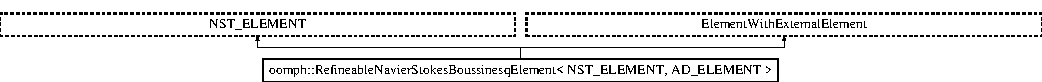
\includegraphics[height=1.098039cm]{classoomph_1_1RefineableNavierStokesBoussinesqElement}
\end{center}
\end{figure}
\subsection*{Public Member Functions}
\begin{DoxyCompactItemize}
\item 
\hyperlink{classoomph_1_1RefineableNavierStokesBoussinesqElement_af9fd72e50fb7d6aaf43bd982ce3de295}{Refineable\+Navier\+Stokes\+Boussinesq\+Element} ()
\begin{DoxyCompactList}\small\item\em Constructor\+: call the underlying constructors and initialise the pointer to the Rayleigh number to point to the default value of 0.\+0. \end{DoxyCompactList}\item 
const double \& \hyperlink{classoomph_1_1RefineableNavierStokesBoussinesqElement_ae18350ad83634633acea59b60123d3c0}{ra} () const
\begin{DoxyCompactList}\small\item\em Access function for the Rayleigh number (const version) \end{DoxyCompactList}\item 
double $\ast$\& \hyperlink{classoomph_1_1RefineableNavierStokesBoussinesqElement_ac2f3ff1714a6859b151da46109eda0ae}{ra\+\_\+pt} ()
\begin{DoxyCompactList}\small\item\em Access function for the pointer to the Rayleigh number. \end{DoxyCompactList}\item 
void \hyperlink{classoomph_1_1RefineableNavierStokesBoussinesqElement_a8b7b18f473b0fa9c4127de305e5a6ccc}{further\+\_\+build} ()
\begin{DoxyCompactList}\small\item\em Call the underlying single-\/physics element\textquotesingle{}s \hyperlink{classoomph_1_1RefineableNavierStokesBoussinesqElement_a8b7b18f473b0fa9c4127de305e5a6ccc}{further\+\_\+build()} functions and make sure that the pointer to the Rayleigh number is passed to the sons. Also make sure that if the external geometric Data was ignored in the father it\textquotesingle{}s also ignored in the sons. \end{DoxyCompactList}\item 
void \hyperlink{classoomph_1_1RefineableNavierStokesBoussinesqElement_a7c422f8666f9acef4d26f187a4dc4e28}{get\+\_\+body\+\_\+force\+\_\+nst} (const double \&time, const unsigned \&ipt, const Vector$<$ double $>$ \&s, const Vector$<$ double $>$ \&x, Vector$<$ double $>$ \&body\+\_\+force)
\begin{DoxyCompactList}\small\item\em Overload \hyperlink{classoomph_1_1RefineableNavierStokesBoussinesqElement_a7c422f8666f9acef4d26f187a4dc4e28}{get\+\_\+body\+\_\+force\+\_\+nst()} to return the temperature-\/dependent buoyancy force, using the temperature computed by the \char`\"{}external\char`\"{} advection diffusion element associated with integration point {\ttfamily ipt}. \end{DoxyCompactList}\item 
void \hyperlink{classoomph_1_1RefineableNavierStokesBoussinesqElement_aab6bae7d0704ab7e3e121ee594ac887a}{fill\+\_\+in\+\_\+contribution\+\_\+to\+\_\+jacobian} (Vector$<$ double $>$ \&residuals, Dense\+Matrix$<$ double $>$ \&jacobian)
\begin{DoxyCompactList}\small\item\em Compute the element\textquotesingle{}s residual vector and the Jacobian matrix. \end{DoxyCompactList}\item 
void \hyperlink{classoomph_1_1RefineableNavierStokesBoussinesqElement_a02e9c7f347aa1c6defbcb20049fc8985}{fill\+\_\+in\+\_\+contribution\+\_\+to\+\_\+jacobian\+\_\+and\+\_\+mass\+\_\+matrix} (Vector$<$ double $>$ \&residuals, Dense\+Matrix$<$ double $>$ \&jacobian, Dense\+Matrix$<$ double $>$ \&mass\+\_\+matrix)
\item 
void \hyperlink{classoomph_1_1RefineableNavierStokesBoussinesqElement_a4450f88be1c003160b9fa99df70a923b}{get\+\_\+dbody\+\_\+force\+\_\+nst\+\_\+dexternal\+\_\+element\+\_\+data} (const unsigned \&ipt, Dense\+Matrix$<$ double $>$ \&result, Vector$<$ unsigned $>$ \&global\+\_\+eqn\+\_\+number)
\begin{DoxyCompactList}\small\item\em Fill in the derivatives of the body force with respect to the external unknowns. \end{DoxyCompactList}\item 
void \hyperlink{classoomph_1_1RefineableNavierStokesBoussinesqElement_a9609dc454ef3d29b1e256fa32fb2c665}{fill\+\_\+in\+\_\+off\+\_\+diagonal\+\_\+block\+\_\+analytic} (Vector$<$ double $>$ \&residuals, Dense\+Matrix$<$ double $>$ \&jacobian)
\begin{DoxyCompactList}\small\item\em Compute the contribution of the external degrees of freedom (temperatures) on the Navier-\/\+Stokes equations. \end{DoxyCompactList}\item 
void \hyperlink{classoomph_1_1RefineableNavierStokesBoussinesqElement_aab581709145cc3e9a4da5c5417d1c50f}{get\+\_\+dof\+\_\+numbers\+\_\+for\+\_\+unknowns} (std\+::list$<$ std\+::pair$<$ unsigned long, unsigned $>$ $>$ \&dof\+\_\+lookup\+\_\+list) const
\begin{DoxyCompactList}\small\item\em Classify dof numbers as in underlying element. \end{DoxyCompactList}\item 
unsigned \hyperlink{classoomph_1_1RefineableNavierStokesBoussinesqElement_a8e494f3887499d79d8c30c7434494b47}{ndof\+\_\+types} () const
\begin{DoxyCompactList}\small\item\em Get number of dof types from underlying element. \end{DoxyCompactList}\end{DoxyCompactItemize}
\subsection*{Private Attributes}
\begin{DoxyCompactItemize}
\item 
double $\ast$ \hyperlink{classoomph_1_1RefineableNavierStokesBoussinesqElement_a4ea4706d0f735b1986287038191ee4e9}{Ra\+\_\+pt}
\begin{DoxyCompactList}\small\item\em Pointer to a private data member, the Rayleigh number. \end{DoxyCompactList}\end{DoxyCompactItemize}


\subsection{Detailed Description}
\subsubsection*{template$<$class N\+S\+T\+\_\+\+E\+L\+E\+M\+E\+NT, class A\+D\+\_\+\+E\+L\+E\+M\+E\+NT$>$\newline
class oomph\+::\+Refineable\+Navier\+Stokes\+Boussinesq\+Element$<$ N\+S\+T\+\_\+\+E\+L\+E\+M\+E\+N\+T, A\+D\+\_\+\+E\+L\+E\+M\+E\+N\+T $>$}

Build a refineable Navier Stokes element that inherits from Element\+With\+External\+Element so that it can \char`\"{}communicate\char`\"{} with an advection diffusion element that provides the temperature in the body force term. 

Definition at line 70 of file multi\+\_\+domain\+\_\+boussinesq\+\_\+elements.\+h.



\subsection{Constructor \& Destructor Documentation}
\mbox{\Hypertarget{classoomph_1_1RefineableNavierStokesBoussinesqElement_af9fd72e50fb7d6aaf43bd982ce3de295}\label{classoomph_1_1RefineableNavierStokesBoussinesqElement_af9fd72e50fb7d6aaf43bd982ce3de295}} 
\index{oomph\+::\+Refineable\+Navier\+Stokes\+Boussinesq\+Element@{oomph\+::\+Refineable\+Navier\+Stokes\+Boussinesq\+Element}!Refineable\+Navier\+Stokes\+Boussinesq\+Element@{Refineable\+Navier\+Stokes\+Boussinesq\+Element}}
\index{Refineable\+Navier\+Stokes\+Boussinesq\+Element@{Refineable\+Navier\+Stokes\+Boussinesq\+Element}!oomph\+::\+Refineable\+Navier\+Stokes\+Boussinesq\+Element@{oomph\+::\+Refineable\+Navier\+Stokes\+Boussinesq\+Element}}
\subsubsection{\texorpdfstring{Refineable\+Navier\+Stokes\+Boussinesq\+Element()}{RefineableNavierStokesBoussinesqElement()}}
{\footnotesize\ttfamily template$<$class N\+S\+T\+\_\+\+E\+L\+E\+M\+E\+NT, class A\+D\+\_\+\+E\+L\+E\+M\+E\+NT$>$ \\
\hyperlink{classoomph_1_1RefineableNavierStokesBoussinesqElement}{oomph\+::\+Refineable\+Navier\+Stokes\+Boussinesq\+Element}$<$ N\+S\+T\+\_\+\+E\+L\+E\+M\+E\+NT, A\+D\+\_\+\+E\+L\+E\+M\+E\+NT $>$\+::\hyperlink{classoomph_1_1RefineableNavierStokesBoussinesqElement}{Refineable\+Navier\+Stokes\+Boussinesq\+Element} (\begin{DoxyParamCaption}{ }\end{DoxyParamCaption})\hspace{0.3cm}{\ttfamily [inline]}}



Constructor\+: call the underlying constructors and initialise the pointer to the Rayleigh number to point to the default value of 0.\+0. 



Definition at line 79 of file multi\+\_\+domain\+\_\+boussinesq\+\_\+elements.\+h.



References oomph\+::\+Multi\+Domain\+Boussinesq\+Helper\+::\+Default\+\_\+\+Physical\+\_\+\+Constant\+\_\+\+Value.



\subsection{Member Function Documentation}
\mbox{\Hypertarget{classoomph_1_1RefineableNavierStokesBoussinesqElement_aab6bae7d0704ab7e3e121ee594ac887a}\label{classoomph_1_1RefineableNavierStokesBoussinesqElement_aab6bae7d0704ab7e3e121ee594ac887a}} 
\index{oomph\+::\+Refineable\+Navier\+Stokes\+Boussinesq\+Element@{oomph\+::\+Refineable\+Navier\+Stokes\+Boussinesq\+Element}!fill\+\_\+in\+\_\+contribution\+\_\+to\+\_\+jacobian@{fill\+\_\+in\+\_\+contribution\+\_\+to\+\_\+jacobian}}
\index{fill\+\_\+in\+\_\+contribution\+\_\+to\+\_\+jacobian@{fill\+\_\+in\+\_\+contribution\+\_\+to\+\_\+jacobian}!oomph\+::\+Refineable\+Navier\+Stokes\+Boussinesq\+Element@{oomph\+::\+Refineable\+Navier\+Stokes\+Boussinesq\+Element}}
\subsubsection{\texorpdfstring{fill\+\_\+in\+\_\+contribution\+\_\+to\+\_\+jacobian()}{fill\_in\_contribution\_to\_jacobian()}}
{\footnotesize\ttfamily template$<$class N\+S\+T\+\_\+\+E\+L\+E\+M\+E\+NT, class A\+D\+\_\+\+E\+L\+E\+M\+E\+NT$>$ \\
void \hyperlink{classoomph_1_1RefineableNavierStokesBoussinesqElement}{oomph\+::\+Refineable\+Navier\+Stokes\+Boussinesq\+Element}$<$ N\+S\+T\+\_\+\+E\+L\+E\+M\+E\+NT, A\+D\+\_\+\+E\+L\+E\+M\+E\+NT $>$\+::fill\+\_\+in\+\_\+contribution\+\_\+to\+\_\+jacobian (\begin{DoxyParamCaption}\item[{Vector$<$ double $>$ \&}]{residuals,  }\item[{Dense\+Matrix$<$ double $>$ \&}]{jacobian }\end{DoxyParamCaption})\hspace{0.3cm}{\ttfamily [inline]}}



Compute the element\textquotesingle{}s residual vector and the Jacobian matrix. 



Definition at line 159 of file multi\+\_\+domain\+\_\+boussinesq\+\_\+elements.\+h.

\mbox{\Hypertarget{classoomph_1_1RefineableNavierStokesBoussinesqElement_a02e9c7f347aa1c6defbcb20049fc8985}\label{classoomph_1_1RefineableNavierStokesBoussinesqElement_a02e9c7f347aa1c6defbcb20049fc8985}} 
\index{oomph\+::\+Refineable\+Navier\+Stokes\+Boussinesq\+Element@{oomph\+::\+Refineable\+Navier\+Stokes\+Boussinesq\+Element}!fill\+\_\+in\+\_\+contribution\+\_\+to\+\_\+jacobian\+\_\+and\+\_\+mass\+\_\+matrix@{fill\+\_\+in\+\_\+contribution\+\_\+to\+\_\+jacobian\+\_\+and\+\_\+mass\+\_\+matrix}}
\index{fill\+\_\+in\+\_\+contribution\+\_\+to\+\_\+jacobian\+\_\+and\+\_\+mass\+\_\+matrix@{fill\+\_\+in\+\_\+contribution\+\_\+to\+\_\+jacobian\+\_\+and\+\_\+mass\+\_\+matrix}!oomph\+::\+Refineable\+Navier\+Stokes\+Boussinesq\+Element@{oomph\+::\+Refineable\+Navier\+Stokes\+Boussinesq\+Element}}
\subsubsection{\texorpdfstring{fill\+\_\+in\+\_\+contribution\+\_\+to\+\_\+jacobian\+\_\+and\+\_\+mass\+\_\+matrix()}{fill\_in\_contribution\_to\_jacobian\_and\_mass\_matrix()}}
{\footnotesize\ttfamily template$<$class N\+S\+T\+\_\+\+E\+L\+E\+M\+E\+NT, class A\+D\+\_\+\+E\+L\+E\+M\+E\+NT$>$ \\
void \hyperlink{classoomph_1_1RefineableNavierStokesBoussinesqElement}{oomph\+::\+Refineable\+Navier\+Stokes\+Boussinesq\+Element}$<$ N\+S\+T\+\_\+\+E\+L\+E\+M\+E\+NT, A\+D\+\_\+\+E\+L\+E\+M\+E\+NT $>$\+::fill\+\_\+in\+\_\+contribution\+\_\+to\+\_\+jacobian\+\_\+and\+\_\+mass\+\_\+matrix (\begin{DoxyParamCaption}\item[{Vector$<$ double $>$ \&}]{residuals,  }\item[{Dense\+Matrix$<$ double $>$ \&}]{jacobian,  }\item[{Dense\+Matrix$<$ double $>$ \&}]{mass\+\_\+matrix }\end{DoxyParamCaption})\hspace{0.3cm}{\ttfamily [inline]}}

Add the element\textquotesingle{}s contribution to its residuals vector, jacobian matrix and mass matrix 

Definition at line 184 of file multi\+\_\+domain\+\_\+boussinesq\+\_\+elements.\+h.

\mbox{\Hypertarget{classoomph_1_1RefineableNavierStokesBoussinesqElement_a9609dc454ef3d29b1e256fa32fb2c665}\label{classoomph_1_1RefineableNavierStokesBoussinesqElement_a9609dc454ef3d29b1e256fa32fb2c665}} 
\index{oomph\+::\+Refineable\+Navier\+Stokes\+Boussinesq\+Element@{oomph\+::\+Refineable\+Navier\+Stokes\+Boussinesq\+Element}!fill\+\_\+in\+\_\+off\+\_\+diagonal\+\_\+block\+\_\+analytic@{fill\+\_\+in\+\_\+off\+\_\+diagonal\+\_\+block\+\_\+analytic}}
\index{fill\+\_\+in\+\_\+off\+\_\+diagonal\+\_\+block\+\_\+analytic@{fill\+\_\+in\+\_\+off\+\_\+diagonal\+\_\+block\+\_\+analytic}!oomph\+::\+Refineable\+Navier\+Stokes\+Boussinesq\+Element@{oomph\+::\+Refineable\+Navier\+Stokes\+Boussinesq\+Element}}
\subsubsection{\texorpdfstring{fill\+\_\+in\+\_\+off\+\_\+diagonal\+\_\+block\+\_\+analytic()}{fill\_in\_off\_diagonal\_block\_analytic()}}
{\footnotesize\ttfamily template$<$class N\+S\+T\+\_\+\+E\+L\+E\+M\+E\+NT, class A\+D\+\_\+\+E\+L\+E\+M\+E\+NT$>$ \\
void \hyperlink{classoomph_1_1RefineableNavierStokesBoussinesqElement}{oomph\+::\+Refineable\+Navier\+Stokes\+Boussinesq\+Element}$<$ N\+S\+T\+\_\+\+E\+L\+E\+M\+E\+NT, A\+D\+\_\+\+E\+L\+E\+M\+E\+NT $>$\+::fill\+\_\+in\+\_\+off\+\_\+diagonal\+\_\+block\+\_\+analytic (\begin{DoxyParamCaption}\item[{Vector$<$ double $>$ \&}]{residuals,  }\item[{Dense\+Matrix$<$ double $>$ \&}]{jacobian }\end{DoxyParamCaption})\hspace{0.3cm}{\ttfamily [inline]}}



Compute the contribution of the external degrees of freedom (temperatures) on the Navier-\/\+Stokes equations. 



Definition at line 205 of file multi\+\_\+domain\+\_\+boussinesq\+\_\+elements.\+h.

\mbox{\Hypertarget{classoomph_1_1RefineableNavierStokesBoussinesqElement_a8b7b18f473b0fa9c4127de305e5a6ccc}\label{classoomph_1_1RefineableNavierStokesBoussinesqElement_a8b7b18f473b0fa9c4127de305e5a6ccc}} 
\index{oomph\+::\+Refineable\+Navier\+Stokes\+Boussinesq\+Element@{oomph\+::\+Refineable\+Navier\+Stokes\+Boussinesq\+Element}!further\+\_\+build@{further\+\_\+build}}
\index{further\+\_\+build@{further\+\_\+build}!oomph\+::\+Refineable\+Navier\+Stokes\+Boussinesq\+Element@{oomph\+::\+Refineable\+Navier\+Stokes\+Boussinesq\+Element}}
\subsubsection{\texorpdfstring{further\+\_\+build()}{further\_build()}}
{\footnotesize\ttfamily template$<$class N\+S\+T\+\_\+\+E\+L\+E\+M\+E\+NT, class A\+D\+\_\+\+E\+L\+E\+M\+E\+NT$>$ \\
void \hyperlink{classoomph_1_1RefineableNavierStokesBoussinesqElement}{oomph\+::\+Refineable\+Navier\+Stokes\+Boussinesq\+Element}$<$ N\+S\+T\+\_\+\+E\+L\+E\+M\+E\+NT, A\+D\+\_\+\+E\+L\+E\+M\+E\+NT $>$\+::further\+\_\+build (\begin{DoxyParamCaption}{ }\end{DoxyParamCaption})\hspace{0.3cm}{\ttfamily [inline]}}



Call the underlying single-\/physics element\textquotesingle{}s \hyperlink{classoomph_1_1RefineableNavierStokesBoussinesqElement_a8b7b18f473b0fa9c4127de305e5a6ccc}{further\+\_\+build()} functions and make sure that the pointer to the Rayleigh number is passed to the sons. Also make sure that if the external geometric Data was ignored in the father it\textquotesingle{}s also ignored in the sons. 



Definition at line 99 of file multi\+\_\+domain\+\_\+boussinesq\+\_\+elements.\+h.



References oomph\+::\+Refineable\+Navier\+Stokes\+Boussinesq\+Element$<$ N\+S\+T\+\_\+\+E\+L\+E\+M\+E\+N\+T, A\+D\+\_\+\+E\+L\+E\+M\+E\+N\+T $>$\+::ra\+\_\+pt().

\mbox{\Hypertarget{classoomph_1_1RefineableNavierStokesBoussinesqElement_a7c422f8666f9acef4d26f187a4dc4e28}\label{classoomph_1_1RefineableNavierStokesBoussinesqElement_a7c422f8666f9acef4d26f187a4dc4e28}} 
\index{oomph\+::\+Refineable\+Navier\+Stokes\+Boussinesq\+Element@{oomph\+::\+Refineable\+Navier\+Stokes\+Boussinesq\+Element}!get\+\_\+body\+\_\+force\+\_\+nst@{get\+\_\+body\+\_\+force\+\_\+nst}}
\index{get\+\_\+body\+\_\+force\+\_\+nst@{get\+\_\+body\+\_\+force\+\_\+nst}!oomph\+::\+Refineable\+Navier\+Stokes\+Boussinesq\+Element@{oomph\+::\+Refineable\+Navier\+Stokes\+Boussinesq\+Element}}
\subsubsection{\texorpdfstring{get\+\_\+body\+\_\+force\+\_\+nst()}{get\_body\_force\_nst()}}
{\footnotesize\ttfamily template$<$class N\+S\+T\+\_\+\+E\+L\+E\+M\+E\+NT, class A\+D\+\_\+\+E\+L\+E\+M\+E\+NT$>$ \\
void \hyperlink{classoomph_1_1RefineableNavierStokesBoussinesqElement}{oomph\+::\+Refineable\+Navier\+Stokes\+Boussinesq\+Element}$<$ N\+S\+T\+\_\+\+E\+L\+E\+M\+E\+NT, A\+D\+\_\+\+E\+L\+E\+M\+E\+NT $>$\+::get\+\_\+body\+\_\+force\+\_\+nst (\begin{DoxyParamCaption}\item[{const double \&}]{time,  }\item[{const unsigned \&}]{ipt,  }\item[{const Vector$<$ double $>$ \&}]{s,  }\item[{const Vector$<$ double $>$ \&}]{x,  }\item[{Vector$<$ double $>$ \&}]{body\+\_\+force }\end{DoxyParamCaption})\hspace{0.3cm}{\ttfamily [inline]}}



Overload \hyperlink{classoomph_1_1RefineableNavierStokesBoussinesqElement_a7c422f8666f9acef4d26f187a4dc4e28}{get\+\_\+body\+\_\+force\+\_\+nst()} to return the temperature-\/dependent buoyancy force, using the temperature computed by the \char`\"{}external\char`\"{} advection diffusion element associated with integration point {\ttfamily ipt}. 



Definition at line 127 of file multi\+\_\+domain\+\_\+boussinesq\+\_\+elements.\+h.

\mbox{\Hypertarget{classoomph_1_1RefineableNavierStokesBoussinesqElement_a4450f88be1c003160b9fa99df70a923b}\label{classoomph_1_1RefineableNavierStokesBoussinesqElement_a4450f88be1c003160b9fa99df70a923b}} 
\index{oomph\+::\+Refineable\+Navier\+Stokes\+Boussinesq\+Element@{oomph\+::\+Refineable\+Navier\+Stokes\+Boussinesq\+Element}!get\+\_\+dbody\+\_\+force\+\_\+nst\+\_\+dexternal\+\_\+element\+\_\+data@{get\+\_\+dbody\+\_\+force\+\_\+nst\+\_\+dexternal\+\_\+element\+\_\+data}}
\index{get\+\_\+dbody\+\_\+force\+\_\+nst\+\_\+dexternal\+\_\+element\+\_\+data@{get\+\_\+dbody\+\_\+force\+\_\+nst\+\_\+dexternal\+\_\+element\+\_\+data}!oomph\+::\+Refineable\+Navier\+Stokes\+Boussinesq\+Element@{oomph\+::\+Refineable\+Navier\+Stokes\+Boussinesq\+Element}}
\subsubsection{\texorpdfstring{get\+\_\+dbody\+\_\+force\+\_\+nst\+\_\+dexternal\+\_\+element\+\_\+data()}{get\_dbody\_force\_nst\_dexternal\_element\_data()}}
{\footnotesize\ttfamily template$<$class N\+S\+T\+\_\+\+E\+L\+E\+M\+E\+NT , class A\+D\+\_\+\+E\+L\+E\+M\+E\+NT $>$ \\
void \hyperlink{classoomph_1_1RefineableNavierStokesBoussinesqElement}{oomph\+::\+Refineable\+Navier\+Stokes\+Boussinesq\+Element}$<$ N\+S\+T\+\_\+\+E\+L\+E\+M\+E\+NT, A\+D\+\_\+\+E\+L\+E\+M\+E\+NT $>$\+::get\+\_\+dbody\+\_\+force\+\_\+nst\+\_\+dexternal\+\_\+element\+\_\+data (\begin{DoxyParamCaption}\item[{const unsigned \&}]{ipt,  }\item[{Dense\+Matrix$<$ double $>$ \&}]{result,  }\item[{Vector$<$ unsigned $>$ \&}]{global\+\_\+eqn\+\_\+number }\end{DoxyParamCaption})}



Fill in the derivatives of the body force with respect to the external unknowns. 

Fill in the derivatives of the body force with respect to the external unknowns in the Navier--Stokes equations 

Definition at line 1404 of file multi\+\_\+domain\+\_\+boussinesq\+\_\+elements.\+h.



Referenced by oomph\+::\+Navier\+Stokes\+Boussinesq\+Element$<$ N\+S\+T\+\_\+\+E\+L\+E\+M\+E\+N\+T, A\+D\+\_\+\+E\+L\+E\+M\+E\+N\+T $>$\+::get\+\_\+dbody\+\_\+force\+\_\+nst\+\_\+dexternal\+\_\+element\+\_\+data().

\mbox{\Hypertarget{classoomph_1_1RefineableNavierStokesBoussinesqElement_aab581709145cc3e9a4da5c5417d1c50f}\label{classoomph_1_1RefineableNavierStokesBoussinesqElement_aab581709145cc3e9a4da5c5417d1c50f}} 
\index{oomph\+::\+Refineable\+Navier\+Stokes\+Boussinesq\+Element@{oomph\+::\+Refineable\+Navier\+Stokes\+Boussinesq\+Element}!get\+\_\+dof\+\_\+numbers\+\_\+for\+\_\+unknowns@{get\+\_\+dof\+\_\+numbers\+\_\+for\+\_\+unknowns}}
\index{get\+\_\+dof\+\_\+numbers\+\_\+for\+\_\+unknowns@{get\+\_\+dof\+\_\+numbers\+\_\+for\+\_\+unknowns}!oomph\+::\+Refineable\+Navier\+Stokes\+Boussinesq\+Element@{oomph\+::\+Refineable\+Navier\+Stokes\+Boussinesq\+Element}}
\subsubsection{\texorpdfstring{get\+\_\+dof\+\_\+numbers\+\_\+for\+\_\+unknowns()}{get\_dof\_numbers\_for\_unknowns()}}
{\footnotesize\ttfamily template$<$class N\+S\+T\+\_\+\+E\+L\+E\+M\+E\+NT, class A\+D\+\_\+\+E\+L\+E\+M\+E\+NT$>$ \\
void \hyperlink{classoomph_1_1RefineableNavierStokesBoussinesqElement}{oomph\+::\+Refineable\+Navier\+Stokes\+Boussinesq\+Element}$<$ N\+S\+T\+\_\+\+E\+L\+E\+M\+E\+NT, A\+D\+\_\+\+E\+L\+E\+M\+E\+NT $>$\+::get\+\_\+dof\+\_\+numbers\+\_\+for\+\_\+unknowns (\begin{DoxyParamCaption}\item[{std\+::list$<$ std\+::pair$<$ unsigned long, unsigned $>$ $>$ \&}]{dof\+\_\+lookup\+\_\+list }\end{DoxyParamCaption}) const\hspace{0.3cm}{\ttfamily [inline]}}



Classify dof numbers as in underlying element. 



Definition at line 346 of file multi\+\_\+domain\+\_\+boussinesq\+\_\+elements.\+h.

\mbox{\Hypertarget{classoomph_1_1RefineableNavierStokesBoussinesqElement_a8e494f3887499d79d8c30c7434494b47}\label{classoomph_1_1RefineableNavierStokesBoussinesqElement_a8e494f3887499d79d8c30c7434494b47}} 
\index{oomph\+::\+Refineable\+Navier\+Stokes\+Boussinesq\+Element@{oomph\+::\+Refineable\+Navier\+Stokes\+Boussinesq\+Element}!ndof\+\_\+types@{ndof\+\_\+types}}
\index{ndof\+\_\+types@{ndof\+\_\+types}!oomph\+::\+Refineable\+Navier\+Stokes\+Boussinesq\+Element@{oomph\+::\+Refineable\+Navier\+Stokes\+Boussinesq\+Element}}
\subsubsection{\texorpdfstring{ndof\+\_\+types()}{ndof\_types()}}
{\footnotesize\ttfamily template$<$class N\+S\+T\+\_\+\+E\+L\+E\+M\+E\+NT, class A\+D\+\_\+\+E\+L\+E\+M\+E\+NT$>$ \\
unsigned \hyperlink{classoomph_1_1RefineableNavierStokesBoussinesqElement}{oomph\+::\+Refineable\+Navier\+Stokes\+Boussinesq\+Element}$<$ N\+S\+T\+\_\+\+E\+L\+E\+M\+E\+NT, A\+D\+\_\+\+E\+L\+E\+M\+E\+NT $>$\+::ndof\+\_\+types (\begin{DoxyParamCaption}{ }\end{DoxyParamCaption}) const\hspace{0.3cm}{\ttfamily [inline]}}



Get number of dof types from underlying element. 



Definition at line 354 of file multi\+\_\+domain\+\_\+boussinesq\+\_\+elements.\+h.

\mbox{\Hypertarget{classoomph_1_1RefineableNavierStokesBoussinesqElement_ae18350ad83634633acea59b60123d3c0}\label{classoomph_1_1RefineableNavierStokesBoussinesqElement_ae18350ad83634633acea59b60123d3c0}} 
\index{oomph\+::\+Refineable\+Navier\+Stokes\+Boussinesq\+Element@{oomph\+::\+Refineable\+Navier\+Stokes\+Boussinesq\+Element}!ra@{ra}}
\index{ra@{ra}!oomph\+::\+Refineable\+Navier\+Stokes\+Boussinesq\+Element@{oomph\+::\+Refineable\+Navier\+Stokes\+Boussinesq\+Element}}
\subsubsection{\texorpdfstring{ra()}{ra()}}
{\footnotesize\ttfamily template$<$class N\+S\+T\+\_\+\+E\+L\+E\+M\+E\+NT, class A\+D\+\_\+\+E\+L\+E\+M\+E\+NT$>$ \\
const double\& \hyperlink{classoomph_1_1RefineableNavierStokesBoussinesqElement}{oomph\+::\+Refineable\+Navier\+Stokes\+Boussinesq\+Element}$<$ N\+S\+T\+\_\+\+E\+L\+E\+M\+E\+NT, A\+D\+\_\+\+E\+L\+E\+M\+E\+NT $>$\+::ra (\begin{DoxyParamCaption}{ }\end{DoxyParamCaption}) const\hspace{0.3cm}{\ttfamily [inline]}}



Access function for the Rayleigh number (const version) 



Definition at line 90 of file multi\+\_\+domain\+\_\+boussinesq\+\_\+elements.\+h.

\mbox{\Hypertarget{classoomph_1_1RefineableNavierStokesBoussinesqElement_ac2f3ff1714a6859b151da46109eda0ae}\label{classoomph_1_1RefineableNavierStokesBoussinesqElement_ac2f3ff1714a6859b151da46109eda0ae}} 
\index{oomph\+::\+Refineable\+Navier\+Stokes\+Boussinesq\+Element@{oomph\+::\+Refineable\+Navier\+Stokes\+Boussinesq\+Element}!ra\+\_\+pt@{ra\+\_\+pt}}
\index{ra\+\_\+pt@{ra\+\_\+pt}!oomph\+::\+Refineable\+Navier\+Stokes\+Boussinesq\+Element@{oomph\+::\+Refineable\+Navier\+Stokes\+Boussinesq\+Element}}
\subsubsection{\texorpdfstring{ra\+\_\+pt()}{ra\_pt()}}
{\footnotesize\ttfamily template$<$class N\+S\+T\+\_\+\+E\+L\+E\+M\+E\+NT, class A\+D\+\_\+\+E\+L\+E\+M\+E\+NT$>$ \\
double$\ast$ \& \hyperlink{classoomph_1_1RefineableNavierStokesBoussinesqElement}{oomph\+::\+Refineable\+Navier\+Stokes\+Boussinesq\+Element}$<$ N\+S\+T\+\_\+\+E\+L\+E\+M\+E\+NT, A\+D\+\_\+\+E\+L\+E\+M\+E\+NT $>$\+::ra\+\_\+pt (\begin{DoxyParamCaption}{ }\end{DoxyParamCaption})\hspace{0.3cm}{\ttfamily [inline]}}



Access function for the pointer to the Rayleigh number. 



Definition at line 93 of file multi\+\_\+domain\+\_\+boussinesq\+\_\+elements.\+h.



Referenced by oomph\+::\+Refineable\+Navier\+Stokes\+Boussinesq\+Element$<$ N\+S\+T\+\_\+\+E\+L\+E\+M\+E\+N\+T, A\+D\+\_\+\+E\+L\+E\+M\+E\+N\+T $>$\+::further\+\_\+build().



\subsection{Member Data Documentation}
\mbox{\Hypertarget{classoomph_1_1RefineableNavierStokesBoussinesqElement_a4ea4706d0f735b1986287038191ee4e9}\label{classoomph_1_1RefineableNavierStokesBoussinesqElement_a4ea4706d0f735b1986287038191ee4e9}} 
\index{oomph\+::\+Refineable\+Navier\+Stokes\+Boussinesq\+Element@{oomph\+::\+Refineable\+Navier\+Stokes\+Boussinesq\+Element}!Ra\+\_\+pt@{Ra\+\_\+pt}}
\index{Ra\+\_\+pt@{Ra\+\_\+pt}!oomph\+::\+Refineable\+Navier\+Stokes\+Boussinesq\+Element@{oomph\+::\+Refineable\+Navier\+Stokes\+Boussinesq\+Element}}
\subsubsection{\texorpdfstring{Ra\+\_\+pt}{Ra\_pt}}
{\footnotesize\ttfamily template$<$class N\+S\+T\+\_\+\+E\+L\+E\+M\+E\+NT, class A\+D\+\_\+\+E\+L\+E\+M\+E\+NT$>$ \\
double$\ast$ \hyperlink{classoomph_1_1RefineableNavierStokesBoussinesqElement}{oomph\+::\+Refineable\+Navier\+Stokes\+Boussinesq\+Element}$<$ N\+S\+T\+\_\+\+E\+L\+E\+M\+E\+NT, A\+D\+\_\+\+E\+L\+E\+M\+E\+NT $>$\+::Ra\+\_\+pt\hspace{0.3cm}{\ttfamily [private]}}



Pointer to a private data member, the Rayleigh number. 



Definition at line 362 of file multi\+\_\+domain\+\_\+boussinesq\+\_\+elements.\+h.



The documentation for this class was generated from the following file\+:\begin{DoxyCompactItemize}
\item 
\hyperlink{multi__domain__boussinesq__elements_8h}{multi\+\_\+domain\+\_\+boussinesq\+\_\+elements.\+h}\end{DoxyCompactItemize}

\hypertarget{classoomph_1_1SegregatableFSIProblem}{}\section{oomph\+:\+:Segregatable\+F\+S\+I\+Problem Class Reference}
\label{classoomph_1_1SegregatableFSIProblem}\index{oomph\+::\+Segregatable\+F\+S\+I\+Problem@{oomph\+::\+Segregatable\+F\+S\+I\+Problem}}


{\ttfamily \#include $<$segregated\+\_\+fsi\+\_\+solver.\+h$>$}

Inheritance diagram for oomph\+:\+:Segregatable\+F\+S\+I\+Problem\+:\begin{figure}[H]
\begin{center}
\leavevmode
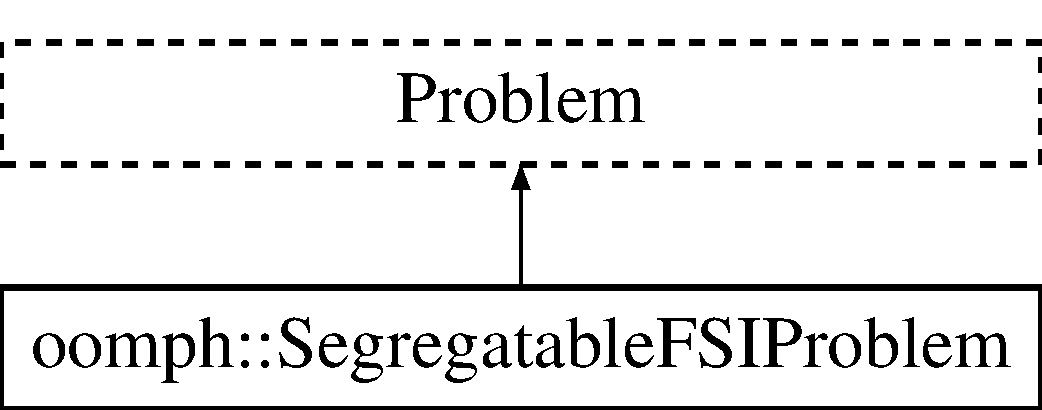
\includegraphics[height=3.000000cm]{classoomph_1_1SegregatableFSIProblem}
\end{center}
\end{figure}
\subsection*{Public Types}
\begin{DoxyCompactItemize}
\item 
enum \hyperlink{classoomph_1_1SegregatableFSIProblem_a06634a6823bb5062d11e97f0be78f373}{convergence\+\_\+criteria} \{ \hyperlink{classoomph_1_1SegregatableFSIProblem_a06634a6823bb5062d11e97f0be78f373a96434fdb328f1440d763eb901f0e1dcc}{Assess\+\_\+convergence\+\_\+based\+\_\+on\+\_\+absolute\+\_\+solid\+\_\+change}, 
\hyperlink{classoomph_1_1SegregatableFSIProblem_a06634a6823bb5062d11e97f0be78f373a735439a264d7a63a310e12f384d5a081}{Assess\+\_\+convergence\+\_\+based\+\_\+on\+\_\+relative\+\_\+solid\+\_\+change}, 
\hyperlink{classoomph_1_1SegregatableFSIProblem_a06634a6823bb5062d11e97f0be78f373aaf32b15e9b1cc097ef3acff8a196bbbd}{Assess\+\_\+convergence\+\_\+based\+\_\+on\+\_\+max\+\_\+global\+\_\+residual}
 \}\begin{DoxyCompactList}\small\item\em Enumerated flags for convergence criteria. \end{DoxyCompactList}
\item 
enum \hyperlink{classoomph_1_1SegregatableFSIProblem_a263f8553427533dc831bd420b8fbf418}{solve\+\_\+type} \{ \hyperlink{classoomph_1_1SegregatableFSIProblem_a263f8553427533dc831bd420b8fbf418a0a2ec06d36907f018f82176e8256e76d}{Full\+\_\+solve}, 
\hyperlink{classoomph_1_1SegregatableFSIProblem_a263f8553427533dc831bd420b8fbf418ab5a200f3f251db5b62d69b7d80b98dae}{Fluid\+\_\+solve}, 
\hyperlink{classoomph_1_1SegregatableFSIProblem_a263f8553427533dc831bd420b8fbf418adb1f2e7a1cc45691468c5a5663ada4ca}{Solid\+\_\+solve}
 \}\begin{DoxyCompactList}\small\item\em Enumerated flags to indicate which solve is taking place. \end{DoxyCompactList}
\end{DoxyCompactItemize}
\subsection*{Public Member Functions}
\begin{DoxyCompactItemize}
\item 
\hyperlink{classoomph_1_1SegregatableFSIProblem_aabbe220c15e7a348a28d54be805ca8d8}{Segregatable\+F\+S\+I\+Problem} ()
\begin{DoxyCompactList}\small\item\em Constructor. Set default values for solver parameters\+: \end{DoxyCompactList}\item 
virtual \hyperlink{classoomph_1_1SegregatableFSIProblem_aa3c69a4078b02d251e4532e73d5820aa}{$\sim$\+Segregatable\+F\+S\+I\+Problem} ()
\begin{DoxyCompactList}\small\item\em Empty virtual destructor. \end{DoxyCompactList}\item 
virtual void \hyperlink{classoomph_1_1SegregatableFSIProblem_a60f719990547949019c8645a4b3a6c6e}{identify\+\_\+fluid\+\_\+and\+\_\+solid\+\_\+dofs} (\hyperlink{classoomph_1_1Vector}{Vector}$<$ \hyperlink{classoomph_1_1Data}{Data} $\ast$$>$ \&fluid\+\_\+data\+\_\+pt, \hyperlink{classoomph_1_1Vector}{Vector}$<$ \hyperlink{classoomph_1_1Data}{Data} $\ast$$>$ \&solid\+\_\+data\+\_\+pt, \hyperlink{classoomph_1_1Mesh}{Mesh} $\ast$\&fluid\+\_\+mesh\+\_\+pt, \hyperlink{classoomph_1_1Mesh}{Mesh} $\ast$\&solid\+\_\+mesh\+\_\+pt)=0
\begin{DoxyCompactList}\small\item\em Identify the fluid and solid \hyperlink{classoomph_1_1Data}{Data}. This is a pure virtual function that M\+U\+ST be implemented for every specific problem that is to be solved by the segregated solver. The two mesh pointers identify meshes that contain elements and nodes used during the fluid or solid solves respectively. Elements that feature during both phases of the segretated solution must be included in both. These pointers may be set to N\+U\+LL. In this case, all elements in the global mesh (set up during the monolithic discretisation of the problem) contribute to the global Jacobian matrix and the residual vector, even if their contributions only contain zero entries. This can be costly, though the code will still compute the correct results. \end{DoxyCompactList}\item 
void \hyperlink{classoomph_1_1SegregatableFSIProblem_a12e662227e5daf656244a531f40022f9}{setup\+\_\+segregated\+\_\+solver} (const bool \&full\+\_\+setup\+\_\+of\+\_\+fluid\+\_\+and\+\_\+solid\+\_\+dofs=true)
\begin{DoxyCompactList}\small\item\em Setup the segregated solver\+: Backup the pinned status of the fluid and solid dofs and allocate the internal storage based on the input provided by identify\+\_\+fluid\+\_\+and\+\_\+solid\+\_\+dofs(...) In addition, reset storage associated with convergence acceleration techniques. If the problem and degrees of freedom has not changed between calls to the solver then it is wasteful to call identify\+\_\+fluid\+\_\+and\+\_\+solid\+\_\+dofs(...) again and again. If the optional boolean flag is set to false then the storage for convergence acceleration techniques is reset, but the fluid and solid dofs are not altered. \end{DoxyCompactList}\item 
\hyperlink{classoomph_1_1PicardConvergenceData}{Picard\+Convergence\+Data} \hyperlink{classoomph_1_1SegregatableFSIProblem_a87a69561674c1e596bb205e0fc4a387f}{segregated\+\_\+solve} ()
\begin{DoxyCompactList}\small\item\em Segregated solver. Peform a segregated step from the present state of the system. Returns \hyperlink{classoomph_1_1PicardConvergenceData}{Picard\+Convergence\+Data} object that contains the vital stats of the iteration. \end{DoxyCompactList}\item 
\hyperlink{classoomph_1_1PicardConvergenceData}{Picard\+Convergence\+Data} \hyperlink{classoomph_1_1SegregatableFSIProblem_a8f8145df86358916df505e2b513caf6a}{steady\+\_\+segregated\+\_\+solve} ()
\begin{DoxyCompactList}\small\item\em \hyperlink{classoomph_1_1Steady}{Steady} version of segregated solver. Makes all timesteppers steady before solving. Returns \hyperlink{classoomph_1_1PicardConvergenceData}{Picard\+Convergence\+Data} object that contains the vital stats of the iteration. \end{DoxyCompactList}\item 
\hyperlink{classoomph_1_1PicardConvergenceData}{Picard\+Convergence\+Data} \hyperlink{classoomph_1_1SegregatableFSIProblem_aae43b43dbc197d238535bcb5c3acf168}{unsteady\+\_\+segregated\+\_\+solve} (const double \&dt)
\begin{DoxyCompactList}\small\item\em Unsteady segregated solver, advance time by dt and solve by the segregated solver. The time values are always shifted by this function. Returns \hyperlink{classoomph_1_1PicardConvergenceData}{Picard\+Convergence\+Data} object that contains the vital stats of the iteration. \end{DoxyCompactList}\item 
\hyperlink{classoomph_1_1PicardConvergenceData}{Picard\+Convergence\+Data} \hyperlink{classoomph_1_1SegregatableFSIProblem_a17f019ebaf83e170219bf605a8554111}{unsteady\+\_\+segregated\+\_\+solve} (const double \&dt, const bool \&shift\+\_\+values)
\begin{DoxyCompactList}\small\item\em Unsteady segregated solver. Advance time by dt and solve the system by a segregated method. The boolean flag is used to control whether the time values should be shifted. If it is true the current data values will be shifted (stored as previous timesteps) before the solution step. Returns \hyperlink{classoomph_1_1PicardConvergenceData}{Picard\+Convergence\+Data} object that contains the vital stats of the iteration. \end{DoxyCompactList}\item 
void \hyperlink{classoomph_1_1SegregatableFSIProblem_a88eb2704f55c89db093cc2857490b727}{assess\+\_\+convergence\+\_\+based\+\_\+on\+\_\+max\+\_\+global\+\_\+residual} (const double \&tol)
\begin{DoxyCompactList}\small\item\em Assess convergence based on max. residual of coupled system of eqns. The argument specifies the convergence tolerance. \end{DoxyCompactList}\item 
void \hyperlink{classoomph_1_1SegregatableFSIProblem_a2fba426552e48abb7ff8a554c20953da}{assess\+\_\+convergence\+\_\+based\+\_\+on\+\_\+max\+\_\+global\+\_\+residual} ()
\begin{DoxyCompactList}\small\item\em Assess convergence based on max. residuals of coupled system of eqns. This interface has no argument and the default convergence tolerance for the Newton solver, \hyperlink{classoomph_1_1Problem_a94536b381e949edf5bb4d44434e08925}{Problem\+::\+Newton\+\_\+solver\+\_\+tolerance} is used. \end{DoxyCompactList}\item 
void \hyperlink{classoomph_1_1SegregatableFSIProblem_aa0b531963389cf3b2ad253891931def9}{assess\+\_\+convergence\+\_\+based\+\_\+on\+\_\+absolute\+\_\+solid\+\_\+change} (const double \&tol)
\begin{DoxyCompactList}\small\item\em Assess convergence based on max. absolute change of solid dofs. The argument specifies the convergence tolerance. \end{DoxyCompactList}\item 
void \hyperlink{classoomph_1_1SegregatableFSIProblem_ae10cc55b3dc502ba387695e8c010b0c1}{assess\+\_\+convergence\+\_\+based\+\_\+on\+\_\+absolute\+\_\+solid\+\_\+change} ()
\begin{DoxyCompactList}\small\item\em Assess convergence based on max. absolute change of solid dofs. This interface has no argument and the default convergence tolerance for the Newton solver, \hyperlink{classoomph_1_1Problem_a94536b381e949edf5bb4d44434e08925}{Problem\+::\+Newton\+\_\+solver\+\_\+tolerance} is used. \end{DoxyCompactList}\item 
void \hyperlink{classoomph_1_1SegregatableFSIProblem_abec6313054e23d998b4584f2de80bc52}{assess\+\_\+convergence\+\_\+based\+\_\+on\+\_\+relative\+\_\+solid\+\_\+change} (const double \&tol)
\begin{DoxyCompactList}\small\item\em Assess convergence based on max. relative change of solid dofs. The argument specifies the convergence tolerance. \end{DoxyCompactList}\item 
void \hyperlink{classoomph_1_1SegregatableFSIProblem_af95d2c3833b64d37635e2e07776cef54}{assess\+\_\+convergence\+\_\+based\+\_\+on\+\_\+relative\+\_\+solid\+\_\+change} ()
\begin{DoxyCompactList}\small\item\em Assess convergence based on max. relative change of solid dofs. This interface has no argument and the default convergence tolerance for the Newton solver, \hyperlink{classoomph_1_1Problem_a94536b381e949edf5bb4d44434e08925}{Problem\+::\+Newton\+\_\+solver\+\_\+tolerance} is used. \end{DoxyCompactList}\item 
void \hyperlink{classoomph_1_1SegregatableFSIProblem_a08c87f24c9e3ea80182a4b19d3a9fa92}{enable\+\_\+pointwise\+\_\+aitken} (const unsigned \&pointwise\+\_\+aitken\+\_\+start)
\begin{DoxyCompactList}\small\item\em Use pointwise Aitken extrapolation. The argument is used to specify the Picard iteration after which pointwise Aitken extrapolation is to be used for the first time. \end{DoxyCompactList}\item 
void \hyperlink{classoomph_1_1SegregatableFSIProblem_a3f52d9c6555b43d8ada274ec80940c13}{enable\+\_\+pointwise\+\_\+aitken} ()
\begin{DoxyCompactList}\small\item\em Use pointwise Aitken extrapolation. This interface has no argument and the current value of Pointwise\+\_\+aitken\+\_\+start will be used. The default is zero, extrapolation starts immediately. \end{DoxyCompactList}\item 
void \hyperlink{classoomph_1_1SegregatableFSIProblem_a34c040b6fe4860ad44bc48ddf859e9fe}{disable\+\_\+pointwise\+\_\+aitken} ()
\begin{DoxyCompactList}\small\item\em Disable the use of pointwise Aitken extrapolation. \end{DoxyCompactList}\item 
void \hyperlink{classoomph_1_1SegregatableFSIProblem_a7ad67f163160a54024fb0bcd5fa531c3}{enable\+\_\+under\+\_\+relaxation} (const double \&omega=1.\+0)
\begin{DoxyCompactList}\small\item\em Use under-\/relaxation and (optionally) specify under-\/relaxation parameter. Default\+: omega=1.\+0 (i.\+e. no actual under-\/relaxation; Other extreme\+: omega=0.\+0 (freeze wall shape). Under-\/relaxation parameter can also be computed dynamically by setting use\+\_\+irons\+\_\+and\+\_\+tuck\+\_\+extrapolation() \end{DoxyCompactList}\item 
void \hyperlink{classoomph_1_1SegregatableFSIProblem_a0cb257e933a9b3e0ce6d9f79a263851f}{enable\+\_\+irons\+\_\+and\+\_\+tuck\+\_\+extrapolation} ()
\begin{DoxyCompactList}\small\item\em Use Irons and Tuck extrapolation for solid dofs. \end{DoxyCompactList}\item 
void \hyperlink{classoomph_1_1SegregatableFSIProblem_a7f0bee5113993bf9b4ce4ab846f49c0a}{disable\+\_\+irons\+\_\+and\+\_\+tuck\+\_\+extrapolation} ()
\begin{DoxyCompactList}\small\item\em Do not use Irons and Tuck extrapolation for solid dofs. \end{DoxyCompactList}\item 
void \hyperlink{classoomph_1_1SegregatableFSIProblem_ad0792ffce87f26d8963846c472f13d08}{get\+\_\+solid\+\_\+change} (double \&rms\+\_\+change, double \&max\+\_\+change, double \&rms\+\_\+norm)
\begin{DoxyCompactList}\small\item\em Get rms of change in the solid dofs; the max. change of the solid dofs and the rms norm of the solid dofs themselves. Change is computed relative to the reference values stored when \hyperlink{classoomph_1_1SegregatableFSIProblem_af6a9e7b6f13b86bf86b65cfb7c4f966f}{store\+\_\+solid\+\_\+dofs()} was last called. \end{DoxyCompactList}\item 
void \hyperlink{classoomph_1_1SegregatableFSIProblem_af6a9e7b6f13b86bf86b65cfb7c4f966f}{store\+\_\+solid\+\_\+dofs} ()
\begin{DoxyCompactList}\small\item\em Store the current solid values as reference values for future convergence check. Also add another entry to pointwise Aitken history if required. \end{DoxyCompactList}\item 
void \hyperlink{classoomph_1_1SegregatableFSIProblem_a61ae984ed6baba413b7577ce1d1b5dc3}{reset\+\_\+timer} ()
\begin{DoxyCompactList}\small\item\em Reset timer. \end{DoxyCompactList}\item 
void \hyperlink{classoomph_1_1SegregatableFSIProblem_a2896156c47a5a6c2e7a390057d394e10}{restart\+\_\+timer} ()
\begin{DoxyCompactList}\small\item\em (Re-\/)start timer (e.\+g. after completing non-\/essential parts of the code such as documentation of the iteration\textquotesingle{}s progress) \end{DoxyCompactList}\item 
void \hyperlink{classoomph_1_1SegregatableFSIProblem_a6282056a5c22b707a1e6c939a3f73dcd}{halt\+\_\+timer} ()
\begin{DoxyCompactList}\small\item\em Halt timer (e.\+g. before performing non-\/essential parts of the code such as documentation of the iteration\textquotesingle{}s progress) \end{DoxyCompactList}\item 
double \hyperlink{classoomph_1_1SegregatableFSIProblem_adaaaa08352182dc5e0a38c7003cb7a6b}{t\+\_\+spent\+\_\+on\+\_\+actual\+\_\+solve} ()
\begin{DoxyCompactList}\small\item\em Total elapsed time since start of solve. \end{DoxyCompactList}\end{DoxyCompactItemize}
\subsection*{Protected Member Functions}
\begin{DoxyCompactItemize}
\item 
virtual void \hyperlink{classoomph_1_1SegregatableFSIProblem_ae8c920185dc95ab3be243276fd4253b0}{actions\+\_\+before\+\_\+segregated\+\_\+solve} ()
\begin{DoxyCompactList}\small\item\em This function is called once at the start of each segregated solve. \end{DoxyCompactList}\item 
virtual void \hyperlink{classoomph_1_1SegregatableFSIProblem_a284fb37276735a73bca0467fa2e44909}{actions\+\_\+after\+\_\+segregated\+\_\+solve} ()
\begin{DoxyCompactList}\small\item\em This function is called once at the end of each segregated solve. \end{DoxyCompactList}\item 
virtual void \hyperlink{classoomph_1_1SegregatableFSIProblem_abc1e909975df69e27f8f1435e215a842}{actions\+\_\+before\+\_\+segregated\+\_\+convergence\+\_\+check} ()
\begin{DoxyCompactList}\small\item\em This function is to be filled with actions that take place before the check for convergence of the entire segregated solve. \end{DoxyCompactList}\item 
void \hyperlink{classoomph_1_1SegregatableFSIProblem_a61cad9a0a75f2999c0529caa9cac2b73}{rebuild\+\_\+monolithic\+\_\+mesh} ()
\begin{DoxyCompactList}\small\item\em Rebuild global mesh for monolithic discretisation. \end{DoxyCompactList}\item 
void \hyperlink{classoomph_1_1SegregatableFSIProblem_abbf4987f2891218d8efcf53de6150425}{restore\+\_\+fluid\+\_\+dofs} ()
\begin{DoxyCompactList}\small\item\em Restore pinned status of fluid dofs. \end{DoxyCompactList}\item 
void \hyperlink{classoomph_1_1SegregatableFSIProblem_acf28573efb54e2b33101ba8cb503a5b8}{pin\+\_\+solid\+\_\+dofs} ()
\begin{DoxyCompactList}\small\item\em Pin solid dofs. \end{DoxyCompactList}\item 
void \hyperlink{classoomph_1_1SegregatableFSIProblem_a6da202671582bf7bf13a3dceb115385f}{restore\+\_\+solid\+\_\+dofs} ()
\begin{DoxyCompactList}\small\item\em Restore pinned status of solid dofs. \end{DoxyCompactList}\item 
void \hyperlink{classoomph_1_1SegregatableFSIProblem_a99a457e1b3c17e9a08590db163eb7118}{pointwise\+\_\+aitken\+\_\+extrapolate} ()
\begin{DoxyCompactList}\small\item\em Do pointwise Aitken extrapolation for solid. \end{DoxyCompactList}\end{DoxyCompactItemize}
\subsection*{Protected Attributes}
\begin{DoxyCompactItemize}
\item 
int \hyperlink{classoomph_1_1SegregatableFSIProblem_ad92eead7c5dc21884292a5a501c71388}{Pointwise\+\_\+aitken\+\_\+counter}
\begin{DoxyCompactList}\small\item\em Number of Aitken histories available (int because after extrapolation it\textquotesingle{}s re-\/initialised to -\/1 to force the computation of three new genuine iterates). \end{DoxyCompactList}\item 
bool \hyperlink{classoomph_1_1SegregatableFSIProblem_a16f0551d5e9dbe5b211bb3b05e80f276}{Use\+\_\+pointwise\+\_\+aitken}
\begin{DoxyCompactList}\small\item\em Use pointwise Aitken extrapolation? \end{DoxyCompactList}\item 
unsigned \hyperlink{classoomph_1_1SegregatableFSIProblem_a47bcf35aed40bbb7e1c3778b8dfad501}{Pointwise\+\_\+aitken\+\_\+start}
\begin{DoxyCompactList}\small\item\em Start pointwise Aitken extrpolation after specified number of Picard iterations. \end{DoxyCompactList}\item 
int \hyperlink{classoomph_1_1SegregatableFSIProblem_af238c6f11f6d4aacd2ff6e0dea917d40}{Solve\+\_\+type}
\begin{DoxyCompactList}\small\item\em Solve that is taking place (enumerated flag) \end{DoxyCompactList}\item 
double \hyperlink{classoomph_1_1SegregatableFSIProblem_ad9f2f249e0886878f096926b2cfca74b}{Convergence\+\_\+tolerance}
\begin{DoxyCompactList}\small\item\em Convergence tolerance for Picard iteration. \end{DoxyCompactList}\item 
unsigned \hyperlink{classoomph_1_1SegregatableFSIProblem_aa2a06cb9517d1f183cdbaa20ea077805}{Max\+\_\+picard}
\begin{DoxyCompactList}\small\item\em Max. number of Picard iterations. \end{DoxyCompactList}\item 
bool \hyperlink{classoomph_1_1SegregatableFSIProblem_aadc0d46511ee90dad36d0d00a8c2d7ad}{Doc\+\_\+max\+\_\+global\+\_\+residual}
\begin{DoxyCompactList}\small\item\em Doc maximum global residual during iteration? (default\+: false) \end{DoxyCompactList}\item 
\hyperlink{classoomph_1_1Vector}{Vector}$<$ \hyperlink{classoomph_1_1Data}{Data} $\ast$ $>$ \hyperlink{classoomph_1_1SegregatableFSIProblem_a1aac015f9f0e9c1b925a534278dc1e55}{Fluid\+\_\+data\+\_\+pt}
\begin{DoxyCompactList}\small\item\em \hyperlink{classoomph_1_1Vector}{Vector} storing the \hyperlink{classoomph_1_1Data}{Data} objects associated with the fluid problem\+: Tyically the nodal and internal data of the elements in the fluid bulk mesh. \end{DoxyCompactList}\item 
\hyperlink{classoomph_1_1Vector}{Vector}$<$ std\+::vector$<$ bool $>$ $>$ \hyperlink{classoomph_1_1SegregatableFSIProblem_aa39b7f8499588b28b9b490771c4bcff2}{Fluid\+\_\+value\+\_\+is\+\_\+pinned}
\begin{DoxyCompactList}\small\item\em \hyperlink{classoomph_1_1Vector}{Vector} of vectors that store the pinned status of fluid \hyperlink{classoomph_1_1Data}{Data} values. \end{DoxyCompactList}\item 
\hyperlink{classoomph_1_1Vector}{Vector}$<$ \hyperlink{classoomph_1_1Data}{Data} $\ast$ $>$ \hyperlink{classoomph_1_1SegregatableFSIProblem_aca9ab5f800334761ae470453ef476067}{Solid\+\_\+data\+\_\+pt}
\begin{DoxyCompactList}\small\item\em \hyperlink{classoomph_1_1Vector}{Vector} storing the \hyperlink{classoomph_1_1Data}{Data} objects associated with the solid problem\+: Typically the positional data of solid nodes and any quantities associated with displacement control, say. \end{DoxyCompactList}\item 
\hyperlink{classoomph_1_1Vector}{Vector}$<$ std\+::vector$<$ bool $>$ $>$ \hyperlink{classoomph_1_1SegregatableFSIProblem_a0f5d6ec62fd33f83600b69c9fcb1f4ed}{Solid\+\_\+value\+\_\+is\+\_\+pinned}
\begin{DoxyCompactList}\small\item\em \hyperlink{classoomph_1_1Vector}{Vector} of vectors that store the pinned status of solid \hyperlink{classoomph_1_1Data}{Data} values. \end{DoxyCompactList}\item 
\hyperlink{classoomph_1_1Vector}{Vector}$<$ double $>$ \hyperlink{classoomph_1_1SegregatableFSIProblem_a6e056ff378e38504d5e9d522820ca8cf}{Previous\+\_\+solid\+\_\+value}
\begin{DoxyCompactList}\small\item\em \hyperlink{classoomph_1_1Vector}{Vector} storing the previous solid values -- used for convergence check. \end{DoxyCompactList}\item 
\hyperlink{classoomph_1_1Mesh}{Mesh} $\ast$ \hyperlink{classoomph_1_1SegregatableFSIProblem_ada29fa4ef2ae7b6460887f8f04eba6bf}{Fluid\+\_\+mesh\+\_\+pt}
\begin{DoxyCompactList}\small\item\em \hyperlink{classoomph_1_1Mesh}{Mesh} containing only fluid elements -- the elements in this \hyperlink{classoomph_1_1Mesh}{Mesh} will be excluded from the assembly process when the solid problem is solved. \end{DoxyCompactList}\item 
\hyperlink{classoomph_1_1Mesh}{Mesh} $\ast$ \hyperlink{classoomph_1_1SegregatableFSIProblem_a3e7f6f5452767279d21ccbfc6336ef12}{Solid\+\_\+mesh\+\_\+pt}
\begin{DoxyCompactList}\small\item\em \hyperlink{classoomph_1_1Mesh}{Mesh} containing only solid elements -- the elements in this mesh will be excluded from the assembly process when the fluid problem is solved. \end{DoxyCompactList}\item 
\hyperlink{classoomph_1_1Vector}{Vector}$<$ \hyperlink{classoomph_1_1Mesh}{Mesh} $\ast$ $>$ \hyperlink{classoomph_1_1SegregatableFSIProblem_a13ff18eb51b4eeb727443931cd19bac9}{Orig\+\_\+sub\+\_\+mesh\+\_\+pt}
\begin{DoxyCompactList}\small\item\em Backup for the pointers to the submeshes in the original problem. \end{DoxyCompactList}\item 
\hyperlink{classoomph_1_1Vector}{Vector}$<$ double $>$ \hyperlink{classoomph_1_1SegregatableFSIProblem_a8f4545c1a2647486d550499aa89e3136}{Del\+\_\+irons\+\_\+and\+\_\+tuck}
\begin{DoxyCompactList}\small\item\em \hyperlink{classoomph_1_1Vector}{Vector} of changes in Irons and Tuck under-\/relaxation. \end{DoxyCompactList}\item 
double \hyperlink{classoomph_1_1SegregatableFSIProblem_a7568103d53df9c84b86fdf41885cf289}{R\+\_\+irons\+\_\+and\+\_\+tuck}
\begin{DoxyCompactList}\small\item\em Irons and Tuck relaxation factor. \end{DoxyCompactList}\item 
\hyperlink{classoomph_1_1Vector}{Vector}$<$ \hyperlink{classoomph_1_1Vector}{Vector}$<$ double $>$ $>$ \hyperlink{classoomph_1_1SegregatableFSIProblem_aa193977e4617aee9906e59bdd31f2263}{Pointwise\+\_\+aitken\+\_\+solid\+\_\+value}
\begin{DoxyCompactList}\small\item\em \hyperlink{classoomph_1_1Vector}{Vector} of Vectors containing up to three previous iterates for the solid dofs; used for pointwise Aitken extrapolation. \end{DoxyCompactList}\item 
bool \hyperlink{classoomph_1_1SegregatableFSIProblem_a0cef79bdf839668a2145e9fe5f77a5f2}{Recheck\+\_\+convergence\+\_\+after\+\_\+pointwise\+\_\+aitken}
\begin{DoxyCompactList}\small\item\em Have we just done a pointwise Aitken step. \end{DoxyCompactList}\end{DoxyCompactItemize}
\subsection*{Private Member Functions}
\begin{DoxyCompactItemize}
\item 
void \hyperlink{classoomph_1_1SegregatableFSIProblem_a0e67b39cdae35ea25ef97e5e768aa60a}{extrapolate\+\_\+solid\+\_\+data} ()
\begin{DoxyCompactList}\small\item\em Extrapolate solid data and update fluid mesh during unsteady run. \end{DoxyCompactList}\item 
void \hyperlink{classoomph_1_1SegregatableFSIProblem_a9da3017952982a64496ff9c16ca7024c}{under\+\_\+relax\+\_\+solid} ()
\begin{DoxyCompactList}\small\item\em Under-\/relax the most recently computed solid variables, either by classical relaxation or by Irons \& Tuck. \end{DoxyCompactList}\item 
void \hyperlink{classoomph_1_1SegregatableFSIProblem_a13a9841e0aa05bf57ec228b49b311a26}{use\+\_\+only\+\_\+fluid\+\_\+elements} ()
\begin{DoxyCompactList}\small\item\em Only include fluid elements in the \hyperlink{classoomph_1_1Problem}{Problem}\textquotesingle{}s mesh. This is called before the segregated fluid solve. The fluid elements are identified by the user via the fluid\+\_\+mesh\+\_\+pt argument in the pure virtual function identify\+\_\+fluid\+\_\+and\+\_\+solid\+\_\+dofs(...). If a N\+U\+LL pointer is returned by this function (i.\+e. if the user hasn\textquotesingle{}t bothered to identify the fluids elements in a submesh, then no stripping of non-\/fluid elements is performed. The result of the computation will be correct but it won\textquotesingle{}t be very efficient. \end{DoxyCompactList}\item 
void \hyperlink{classoomph_1_1SegregatableFSIProblem_a330660bc7b69c9c128bfed62b54dcf62}{use\+\_\+only\+\_\+solid\+\_\+elements} ()
\begin{DoxyCompactList}\small\item\em Only include solid elements in the \hyperlink{classoomph_1_1Problem}{Problem}\textquotesingle{}s mesh. This is called before the segregated solid solve. The solid elements are identified by the user via the solid\+\_\+mesh\+\_\+pt argument in the pure virtual function identify\+\_\+fluid\+\_\+and\+\_\+solid\+\_\+dofs(...). If a N\+U\+LL pointer is returned by this function (i.\+e. if the user hasn\textquotesingle{}t bothered to identify the solid elements in a submesh, then no stripping of non-\/solid elements is performed. The result of the computation will be correct but it won\textquotesingle{}t be very efficient. \end{DoxyCompactList}\item 
void \hyperlink{classoomph_1_1SegregatableFSIProblem_a33397ef8c5410b782cc9801979812be0}{pin\+\_\+fluid\+\_\+dofs} ()
\begin{DoxyCompactList}\small\item\em Pin fluid dofs. \end{DoxyCompactList}\end{DoxyCompactItemize}
\subsection*{Private Attributes}
\begin{DoxyCompactItemize}
\item 
double \hyperlink{classoomph_1_1SegregatableFSIProblem_adc81fa8a44920be1b41dcea5008db7ed}{Omega\+\_\+relax}
\begin{DoxyCompactList}\small\item\em Under-\/relaxation parameter. (1.\+0\+: no under-\/relaxation; 0.\+0\+: Freeze wall shape) \end{DoxyCompactList}\item 
bool \hyperlink{classoomph_1_1SegregatableFSIProblem_a23930085f18e43926b6afcbbdd2a0509}{Use\+\_\+irons\+\_\+and\+\_\+tuck\+\_\+extrapolation}
\begin{DoxyCompactList}\small\item\em Boolean flag to indicate use of Irons and Tuck\textquotesingle{}s extrapolation for solid values. \end{DoxyCompactList}\item 
int \hyperlink{classoomph_1_1SegregatableFSIProblem_a971ddd09518a1771ae3a6ed85a51514e}{Convergence\+\_\+criterion}
\begin{DoxyCompactList}\small\item\em Convergence criterion (enumerated flag) \end{DoxyCompactList}\item 
clock\+\_\+t \hyperlink{classoomph_1_1SegregatableFSIProblem_a814254917e5cedc6fce1793168124beb}{T\+\_\+ref}
\begin{DoxyCompactList}\small\item\em Reference time for segregated solve. Can be re-\/initialised whenever total elapsed time has been stored (before entering non-\/essential doc sections of the code) \end{DoxyCompactList}\item 
double \hyperlink{classoomph_1_1SegregatableFSIProblem_a8043214c2864bd7584f40e684dcceb58}{T\+\_\+spent\+\_\+on\+\_\+actual\+\_\+solve}
\begin{DoxyCompactList}\small\item\em Total elapsed time since start of solve, can be accumulated by adding bits of time spent in relevant parts of code (bypassing sections that only document the progress) \end{DoxyCompactList}\item 
bool \hyperlink{classoomph_1_1SegregatableFSIProblem_abb20be243e501b04b18da8697ce0985d}{Timer\+\_\+has\+\_\+been\+\_\+halted}
\begin{DoxyCompactList}\small\item\em boolean flag to indicate if timer has been halted \end{DoxyCompactList}\end{DoxyCompactItemize}
\subsection*{Additional Inherited Members}


\subsection{Detailed Description}
Base class for problems that can be solved by segregated F\+SI solver 

Definition at line 153 of file segregated\+\_\+fsi\+\_\+solver.\+h.



\subsection{Member Enumeration Documentation}
\mbox{\Hypertarget{classoomph_1_1SegregatableFSIProblem_a06634a6823bb5062d11e97f0be78f373}\label{classoomph_1_1SegregatableFSIProblem_a06634a6823bb5062d11e97f0be78f373}} 
\index{oomph\+::\+Segregatable\+F\+S\+I\+Problem@{oomph\+::\+Segregatable\+F\+S\+I\+Problem}!convergence\+\_\+criteria@{convergence\+\_\+criteria}}
\index{convergence\+\_\+criteria@{convergence\+\_\+criteria}!oomph\+::\+Segregatable\+F\+S\+I\+Problem@{oomph\+::\+Segregatable\+F\+S\+I\+Problem}}
\subsubsection{\texorpdfstring{convergence\+\_\+criteria}{convergence\_criteria}}
{\footnotesize\ttfamily enum \hyperlink{classoomph_1_1SegregatableFSIProblem_a06634a6823bb5062d11e97f0be78f373}{oomph\+::\+Segregatable\+F\+S\+I\+Problem\+::convergence\+\_\+criteria}}



Enumerated flags for convergence criteria. 

\begin{DoxyEnumFields}{Enumerator}
\raisebox{\heightof{T}}[0pt][0pt]{\index{Assess\+\_\+convergence\+\_\+based\+\_\+on\+\_\+absolute\+\_\+solid\+\_\+change@{Assess\+\_\+convergence\+\_\+based\+\_\+on\+\_\+absolute\+\_\+solid\+\_\+change}!oomph\+::\+Segregatable\+F\+S\+I\+Problem@{oomph\+::\+Segregatable\+F\+S\+I\+Problem}}\index{oomph\+::\+Segregatable\+F\+S\+I\+Problem@{oomph\+::\+Segregatable\+F\+S\+I\+Problem}!Assess\+\_\+convergence\+\_\+based\+\_\+on\+\_\+absolute\+\_\+solid\+\_\+change@{Assess\+\_\+convergence\+\_\+based\+\_\+on\+\_\+absolute\+\_\+solid\+\_\+change}}}\mbox{\Hypertarget{classoomph_1_1SegregatableFSIProblem_a06634a6823bb5062d11e97f0be78f373a96434fdb328f1440d763eb901f0e1dcc}\label{classoomph_1_1SegregatableFSIProblem_a06634a6823bb5062d11e97f0be78f373a96434fdb328f1440d763eb901f0e1dcc}} 
Assess\+\_\+convergence\+\_\+based\+\_\+on\+\_\+absolute\+\_\+solid\+\_\+change&\\
\hline

\raisebox{\heightof{T}}[0pt][0pt]{\index{Assess\+\_\+convergence\+\_\+based\+\_\+on\+\_\+relative\+\_\+solid\+\_\+change@{Assess\+\_\+convergence\+\_\+based\+\_\+on\+\_\+relative\+\_\+solid\+\_\+change}!oomph\+::\+Segregatable\+F\+S\+I\+Problem@{oomph\+::\+Segregatable\+F\+S\+I\+Problem}}\index{oomph\+::\+Segregatable\+F\+S\+I\+Problem@{oomph\+::\+Segregatable\+F\+S\+I\+Problem}!Assess\+\_\+convergence\+\_\+based\+\_\+on\+\_\+relative\+\_\+solid\+\_\+change@{Assess\+\_\+convergence\+\_\+based\+\_\+on\+\_\+relative\+\_\+solid\+\_\+change}}}\mbox{\Hypertarget{classoomph_1_1SegregatableFSIProblem_a06634a6823bb5062d11e97f0be78f373a735439a264d7a63a310e12f384d5a081}\label{classoomph_1_1SegregatableFSIProblem_a06634a6823bb5062d11e97f0be78f373a735439a264d7a63a310e12f384d5a081}} 
Assess\+\_\+convergence\+\_\+based\+\_\+on\+\_\+relative\+\_\+solid\+\_\+change&\\
\hline

\raisebox{\heightof{T}}[0pt][0pt]{\index{Assess\+\_\+convergence\+\_\+based\+\_\+on\+\_\+max\+\_\+global\+\_\+residual@{Assess\+\_\+convergence\+\_\+based\+\_\+on\+\_\+max\+\_\+global\+\_\+residual}!oomph\+::\+Segregatable\+F\+S\+I\+Problem@{oomph\+::\+Segregatable\+F\+S\+I\+Problem}}\index{oomph\+::\+Segregatable\+F\+S\+I\+Problem@{oomph\+::\+Segregatable\+F\+S\+I\+Problem}!Assess\+\_\+convergence\+\_\+based\+\_\+on\+\_\+max\+\_\+global\+\_\+residual@{Assess\+\_\+convergence\+\_\+based\+\_\+on\+\_\+max\+\_\+global\+\_\+residual}}}\mbox{\Hypertarget{classoomph_1_1SegregatableFSIProblem_a06634a6823bb5062d11e97f0be78f373aaf32b15e9b1cc097ef3acff8a196bbbd}\label{classoomph_1_1SegregatableFSIProblem_a06634a6823bb5062d11e97f0be78f373aaf32b15e9b1cc097ef3acff8a196bbbd}} 
Assess\+\_\+convergence\+\_\+based\+\_\+on\+\_\+max\+\_\+global\+\_\+residual&\\
\hline

\end{DoxyEnumFields}


Definition at line 389 of file segregated\+\_\+fsi\+\_\+solver.\+h.

\mbox{\Hypertarget{classoomph_1_1SegregatableFSIProblem_a263f8553427533dc831bd420b8fbf418}\label{classoomph_1_1SegregatableFSIProblem_a263f8553427533dc831bd420b8fbf418}} 
\index{oomph\+::\+Segregatable\+F\+S\+I\+Problem@{oomph\+::\+Segregatable\+F\+S\+I\+Problem}!solve\+\_\+type@{solve\+\_\+type}}
\index{solve\+\_\+type@{solve\+\_\+type}!oomph\+::\+Segregatable\+F\+S\+I\+Problem@{oomph\+::\+Segregatable\+F\+S\+I\+Problem}}
\subsubsection{\texorpdfstring{solve\+\_\+type}{solve\_type}}
{\footnotesize\ttfamily enum \hyperlink{classoomph_1_1SegregatableFSIProblem_a263f8553427533dc831bd420b8fbf418}{oomph\+::\+Segregatable\+F\+S\+I\+Problem\+::solve\+\_\+type}}



Enumerated flags to indicate which solve is taking place. 

\begin{DoxyEnumFields}{Enumerator}
\raisebox{\heightof{T}}[0pt][0pt]{\index{Full\+\_\+solve@{Full\+\_\+solve}!oomph\+::\+Segregatable\+F\+S\+I\+Problem@{oomph\+::\+Segregatable\+F\+S\+I\+Problem}}\index{oomph\+::\+Segregatable\+F\+S\+I\+Problem@{oomph\+::\+Segregatable\+F\+S\+I\+Problem}!Full\+\_\+solve@{Full\+\_\+solve}}}\mbox{\Hypertarget{classoomph_1_1SegregatableFSIProblem_a263f8553427533dc831bd420b8fbf418a0a2ec06d36907f018f82176e8256e76d}\label{classoomph_1_1SegregatableFSIProblem_a263f8553427533dc831bd420b8fbf418a0a2ec06d36907f018f82176e8256e76d}} 
Full\+\_\+solve&\\
\hline

\raisebox{\heightof{T}}[0pt][0pt]{\index{Fluid\+\_\+solve@{Fluid\+\_\+solve}!oomph\+::\+Segregatable\+F\+S\+I\+Problem@{oomph\+::\+Segregatable\+F\+S\+I\+Problem}}\index{oomph\+::\+Segregatable\+F\+S\+I\+Problem@{oomph\+::\+Segregatable\+F\+S\+I\+Problem}!Fluid\+\_\+solve@{Fluid\+\_\+solve}}}\mbox{\Hypertarget{classoomph_1_1SegregatableFSIProblem_a263f8553427533dc831bd420b8fbf418ab5a200f3f251db5b62d69b7d80b98dae}\label{classoomph_1_1SegregatableFSIProblem_a263f8553427533dc831bd420b8fbf418ab5a200f3f251db5b62d69b7d80b98dae}} 
Fluid\+\_\+solve&\\
\hline

\raisebox{\heightof{T}}[0pt][0pt]{\index{Solid\+\_\+solve@{Solid\+\_\+solve}!oomph\+::\+Segregatable\+F\+S\+I\+Problem@{oomph\+::\+Segregatable\+F\+S\+I\+Problem}}\index{oomph\+::\+Segregatable\+F\+S\+I\+Problem@{oomph\+::\+Segregatable\+F\+S\+I\+Problem}!Solid\+\_\+solve@{Solid\+\_\+solve}}}\mbox{\Hypertarget{classoomph_1_1SegregatableFSIProblem_a263f8553427533dc831bd420b8fbf418adb1f2e7a1cc45691468c5a5663ada4ca}\label{classoomph_1_1SegregatableFSIProblem_a263f8553427533dc831bd420b8fbf418adb1f2e7a1cc45691468c5a5663ada4ca}} 
Solid\+\_\+solve&\\
\hline

\end{DoxyEnumFields}


Definition at line 395 of file segregated\+\_\+fsi\+\_\+solver.\+h.



\subsection{Constructor \& Destructor Documentation}
\mbox{\Hypertarget{classoomph_1_1SegregatableFSIProblem_aabbe220c15e7a348a28d54be805ca8d8}\label{classoomph_1_1SegregatableFSIProblem_aabbe220c15e7a348a28d54be805ca8d8}} 
\index{oomph\+::\+Segregatable\+F\+S\+I\+Problem@{oomph\+::\+Segregatable\+F\+S\+I\+Problem}!Segregatable\+F\+S\+I\+Problem@{Segregatable\+F\+S\+I\+Problem}}
\index{Segregatable\+F\+S\+I\+Problem@{Segregatable\+F\+S\+I\+Problem}!oomph\+::\+Segregatable\+F\+S\+I\+Problem@{oomph\+::\+Segregatable\+F\+S\+I\+Problem}}
\subsubsection{\texorpdfstring{Segregatable\+F\+S\+I\+Problem()}{SegregatableFSIProblem()}}
{\footnotesize\ttfamily oomph\+::\+Segregatable\+F\+S\+I\+Problem\+::\+Segregatable\+F\+S\+I\+Problem (\begin{DoxyParamCaption}{ }\end{DoxyParamCaption})\hspace{0.3cm}{\ttfamily [inline]}}



Constructor. Set default values for solver parameters\+: 


\begin{DoxyItemize}
\item Don\textquotesingle{}t use pointwise Aitken extrapolation but if it\textquotesingle{}s used at all, it\textquotesingle{}s used immediately.
\item No under-\/relaxation at all (neither classical nor Irons\&Tuck)
\item Base convergence on max. residual of coupled system of eqns
\item Convergence tolerance = tolerance for Newton solver defined in \hyperlink{classoomph_1_1Problem}{Problem} base class
\item Max. 50 Picard iterations 
\end{DoxyItemize}boolean flag to indicate if timer has been halted 

Definition at line 179 of file segregated\+\_\+fsi\+\_\+solver.\+h.



References oomph\+::\+Problem\+::\+Newton\+\_\+solver\+\_\+tolerance.

\mbox{\Hypertarget{classoomph_1_1SegregatableFSIProblem_aa3c69a4078b02d251e4532e73d5820aa}\label{classoomph_1_1SegregatableFSIProblem_aa3c69a4078b02d251e4532e73d5820aa}} 
\index{oomph\+::\+Segregatable\+F\+S\+I\+Problem@{oomph\+::\+Segregatable\+F\+S\+I\+Problem}!````~Segregatable\+F\+S\+I\+Problem@{$\sim$\+Segregatable\+F\+S\+I\+Problem}}
\index{````~Segregatable\+F\+S\+I\+Problem@{$\sim$\+Segregatable\+F\+S\+I\+Problem}!oomph\+::\+Segregatable\+F\+S\+I\+Problem@{oomph\+::\+Segregatable\+F\+S\+I\+Problem}}
\subsubsection{\texorpdfstring{$\sim$\+Segregatable\+F\+S\+I\+Problem()}{~SegregatableFSIProblem()}}
{\footnotesize\ttfamily virtual oomph\+::\+Segregatable\+F\+S\+I\+Problem\+::$\sim$\+Segregatable\+F\+S\+I\+Problem (\begin{DoxyParamCaption}{ }\end{DoxyParamCaption})\hspace{0.3cm}{\ttfamily [inline]}, {\ttfamily [virtual]}}



Empty virtual destructor. 



Definition at line 230 of file segregated\+\_\+fsi\+\_\+solver.\+h.



\subsection{Member Function Documentation}
\mbox{\Hypertarget{classoomph_1_1SegregatableFSIProblem_a284fb37276735a73bca0467fa2e44909}\label{classoomph_1_1SegregatableFSIProblem_a284fb37276735a73bca0467fa2e44909}} 
\index{oomph\+::\+Segregatable\+F\+S\+I\+Problem@{oomph\+::\+Segregatable\+F\+S\+I\+Problem}!actions\+\_\+after\+\_\+segregated\+\_\+solve@{actions\+\_\+after\+\_\+segregated\+\_\+solve}}
\index{actions\+\_\+after\+\_\+segregated\+\_\+solve@{actions\+\_\+after\+\_\+segregated\+\_\+solve}!oomph\+::\+Segregatable\+F\+S\+I\+Problem@{oomph\+::\+Segregatable\+F\+S\+I\+Problem}}
\subsubsection{\texorpdfstring{actions\+\_\+after\+\_\+segregated\+\_\+solve()}{actions\_after\_segregated\_solve()}}
{\footnotesize\ttfamily virtual void oomph\+::\+Segregatable\+F\+S\+I\+Problem\+::actions\+\_\+after\+\_\+segregated\+\_\+solve (\begin{DoxyParamCaption}{ }\end{DoxyParamCaption})\hspace{0.3cm}{\ttfamily [inline]}, {\ttfamily [protected]}, {\ttfamily [virtual]}}



This function is called once at the end of each segregated solve. 



Definition at line 163 of file segregated\+\_\+fsi\+\_\+solver.\+h.



Referenced by segregated\+\_\+solve().

\mbox{\Hypertarget{classoomph_1_1SegregatableFSIProblem_abc1e909975df69e27f8f1435e215a842}\label{classoomph_1_1SegregatableFSIProblem_abc1e909975df69e27f8f1435e215a842}} 
\index{oomph\+::\+Segregatable\+F\+S\+I\+Problem@{oomph\+::\+Segregatable\+F\+S\+I\+Problem}!actions\+\_\+before\+\_\+segregated\+\_\+convergence\+\_\+check@{actions\+\_\+before\+\_\+segregated\+\_\+convergence\+\_\+check}}
\index{actions\+\_\+before\+\_\+segregated\+\_\+convergence\+\_\+check@{actions\+\_\+before\+\_\+segregated\+\_\+convergence\+\_\+check}!oomph\+::\+Segregatable\+F\+S\+I\+Problem@{oomph\+::\+Segregatable\+F\+S\+I\+Problem}}
\subsubsection{\texorpdfstring{actions\+\_\+before\+\_\+segregated\+\_\+convergence\+\_\+check()}{actions\_before\_segregated\_convergence\_check()}}
{\footnotesize\ttfamily virtual void oomph\+::\+Segregatable\+F\+S\+I\+Problem\+::actions\+\_\+before\+\_\+segregated\+\_\+convergence\+\_\+check (\begin{DoxyParamCaption}{ }\end{DoxyParamCaption})\hspace{0.3cm}{\ttfamily [inline]}, {\ttfamily [protected]}, {\ttfamily [virtual]}}



This function is to be filled with actions that take place before the check for convergence of the entire segregated solve. 



Definition at line 167 of file segregated\+\_\+fsi\+\_\+solver.\+h.



Referenced by segregated\+\_\+solve().

\mbox{\Hypertarget{classoomph_1_1SegregatableFSIProblem_ae8c920185dc95ab3be243276fd4253b0}\label{classoomph_1_1SegregatableFSIProblem_ae8c920185dc95ab3be243276fd4253b0}} 
\index{oomph\+::\+Segregatable\+F\+S\+I\+Problem@{oomph\+::\+Segregatable\+F\+S\+I\+Problem}!actions\+\_\+before\+\_\+segregated\+\_\+solve@{actions\+\_\+before\+\_\+segregated\+\_\+solve}}
\index{actions\+\_\+before\+\_\+segregated\+\_\+solve@{actions\+\_\+before\+\_\+segregated\+\_\+solve}!oomph\+::\+Segregatable\+F\+S\+I\+Problem@{oomph\+::\+Segregatable\+F\+S\+I\+Problem}}
\subsubsection{\texorpdfstring{actions\+\_\+before\+\_\+segregated\+\_\+solve()}{actions\_before\_segregated\_solve()}}
{\footnotesize\ttfamily virtual void oomph\+::\+Segregatable\+F\+S\+I\+Problem\+::actions\+\_\+before\+\_\+segregated\+\_\+solve (\begin{DoxyParamCaption}{ }\end{DoxyParamCaption})\hspace{0.3cm}{\ttfamily [inline]}, {\ttfamily [protected]}, {\ttfamily [virtual]}}



This function is called once at the start of each segregated solve. 



Definition at line 159 of file segregated\+\_\+fsi\+\_\+solver.\+h.



Referenced by segregated\+\_\+solve().

\mbox{\Hypertarget{classoomph_1_1SegregatableFSIProblem_aa0b531963389cf3b2ad253891931def9}\label{classoomph_1_1SegregatableFSIProblem_aa0b531963389cf3b2ad253891931def9}} 
\index{oomph\+::\+Segregatable\+F\+S\+I\+Problem@{oomph\+::\+Segregatable\+F\+S\+I\+Problem}!assess\+\_\+convergence\+\_\+based\+\_\+on\+\_\+absolute\+\_\+solid\+\_\+change@{assess\+\_\+convergence\+\_\+based\+\_\+on\+\_\+absolute\+\_\+solid\+\_\+change}}
\index{assess\+\_\+convergence\+\_\+based\+\_\+on\+\_\+absolute\+\_\+solid\+\_\+change@{assess\+\_\+convergence\+\_\+based\+\_\+on\+\_\+absolute\+\_\+solid\+\_\+change}!oomph\+::\+Segregatable\+F\+S\+I\+Problem@{oomph\+::\+Segregatable\+F\+S\+I\+Problem}}
\subsubsection{\texorpdfstring{assess\+\_\+convergence\+\_\+based\+\_\+on\+\_\+absolute\+\_\+solid\+\_\+change()}{assess\_convergence\_based\_on\_absolute\_solid\_change()}\hspace{0.1cm}{\footnotesize\ttfamily [1/2]}}
{\footnotesize\ttfamily void oomph\+::\+Segregatable\+F\+S\+I\+Problem\+::assess\+\_\+convergence\+\_\+based\+\_\+on\+\_\+absolute\+\_\+solid\+\_\+change (\begin{DoxyParamCaption}\item[{const double \&}]{tol }\end{DoxyParamCaption})\hspace{0.3cm}{\ttfamily [inline]}}



Assess convergence based on max. absolute change of solid dofs. The argument specifies the convergence tolerance. 



Definition at line 318 of file segregated\+\_\+fsi\+\_\+solver.\+h.

\mbox{\Hypertarget{classoomph_1_1SegregatableFSIProblem_ae10cc55b3dc502ba387695e8c010b0c1}\label{classoomph_1_1SegregatableFSIProblem_ae10cc55b3dc502ba387695e8c010b0c1}} 
\index{oomph\+::\+Segregatable\+F\+S\+I\+Problem@{oomph\+::\+Segregatable\+F\+S\+I\+Problem}!assess\+\_\+convergence\+\_\+based\+\_\+on\+\_\+absolute\+\_\+solid\+\_\+change@{assess\+\_\+convergence\+\_\+based\+\_\+on\+\_\+absolute\+\_\+solid\+\_\+change}}
\index{assess\+\_\+convergence\+\_\+based\+\_\+on\+\_\+absolute\+\_\+solid\+\_\+change@{assess\+\_\+convergence\+\_\+based\+\_\+on\+\_\+absolute\+\_\+solid\+\_\+change}!oomph\+::\+Segregatable\+F\+S\+I\+Problem@{oomph\+::\+Segregatable\+F\+S\+I\+Problem}}
\subsubsection{\texorpdfstring{assess\+\_\+convergence\+\_\+based\+\_\+on\+\_\+absolute\+\_\+solid\+\_\+change()}{assess\_convergence\_based\_on\_absolute\_solid\_change()}\hspace{0.1cm}{\footnotesize\ttfamily [2/2]}}
{\footnotesize\ttfamily void oomph\+::\+Segregatable\+F\+S\+I\+Problem\+::assess\+\_\+convergence\+\_\+based\+\_\+on\+\_\+absolute\+\_\+solid\+\_\+change (\begin{DoxyParamCaption}{ }\end{DoxyParamCaption})\hspace{0.3cm}{\ttfamily [inline]}}



Assess convergence based on max. absolute change of solid dofs. This interface has no argument and the default convergence tolerance for the Newton solver, \hyperlink{classoomph_1_1Problem_a94536b381e949edf5bb4d44434e08925}{Problem\+::\+Newton\+\_\+solver\+\_\+tolerance} is used. 



Definition at line 329 of file segregated\+\_\+fsi\+\_\+solver.\+h.



References oomph\+::\+Problem\+::\+Newton\+\_\+solver\+\_\+tolerance.

\mbox{\Hypertarget{classoomph_1_1SegregatableFSIProblem_a88eb2704f55c89db093cc2857490b727}\label{classoomph_1_1SegregatableFSIProblem_a88eb2704f55c89db093cc2857490b727}} 
\index{oomph\+::\+Segregatable\+F\+S\+I\+Problem@{oomph\+::\+Segregatable\+F\+S\+I\+Problem}!assess\+\_\+convergence\+\_\+based\+\_\+on\+\_\+max\+\_\+global\+\_\+residual@{assess\+\_\+convergence\+\_\+based\+\_\+on\+\_\+max\+\_\+global\+\_\+residual}}
\index{assess\+\_\+convergence\+\_\+based\+\_\+on\+\_\+max\+\_\+global\+\_\+residual@{assess\+\_\+convergence\+\_\+based\+\_\+on\+\_\+max\+\_\+global\+\_\+residual}!oomph\+::\+Segregatable\+F\+S\+I\+Problem@{oomph\+::\+Segregatable\+F\+S\+I\+Problem}}
\subsubsection{\texorpdfstring{assess\+\_\+convergence\+\_\+based\+\_\+on\+\_\+max\+\_\+global\+\_\+residual()}{assess\_convergence\_based\_on\_max\_global\_residual()}\hspace{0.1cm}{\footnotesize\ttfamily [1/2]}}
{\footnotesize\ttfamily void oomph\+::\+Segregatable\+F\+S\+I\+Problem\+::assess\+\_\+convergence\+\_\+based\+\_\+on\+\_\+max\+\_\+global\+\_\+residual (\begin{DoxyParamCaption}\item[{const double \&}]{tol }\end{DoxyParamCaption})\hspace{0.3cm}{\ttfamily [inline]}}



Assess convergence based on max. residual of coupled system of eqns. The argument specifies the convergence tolerance. 



Definition at line 299 of file segregated\+\_\+fsi\+\_\+solver.\+h.

\mbox{\Hypertarget{classoomph_1_1SegregatableFSIProblem_a2fba426552e48abb7ff8a554c20953da}\label{classoomph_1_1SegregatableFSIProblem_a2fba426552e48abb7ff8a554c20953da}} 
\index{oomph\+::\+Segregatable\+F\+S\+I\+Problem@{oomph\+::\+Segregatable\+F\+S\+I\+Problem}!assess\+\_\+convergence\+\_\+based\+\_\+on\+\_\+max\+\_\+global\+\_\+residual@{assess\+\_\+convergence\+\_\+based\+\_\+on\+\_\+max\+\_\+global\+\_\+residual}}
\index{assess\+\_\+convergence\+\_\+based\+\_\+on\+\_\+max\+\_\+global\+\_\+residual@{assess\+\_\+convergence\+\_\+based\+\_\+on\+\_\+max\+\_\+global\+\_\+residual}!oomph\+::\+Segregatable\+F\+S\+I\+Problem@{oomph\+::\+Segregatable\+F\+S\+I\+Problem}}
\subsubsection{\texorpdfstring{assess\+\_\+convergence\+\_\+based\+\_\+on\+\_\+max\+\_\+global\+\_\+residual()}{assess\_convergence\_based\_on\_max\_global\_residual()}\hspace{0.1cm}{\footnotesize\ttfamily [2/2]}}
{\footnotesize\ttfamily void oomph\+::\+Segregatable\+F\+S\+I\+Problem\+::assess\+\_\+convergence\+\_\+based\+\_\+on\+\_\+max\+\_\+global\+\_\+residual (\begin{DoxyParamCaption}{ }\end{DoxyParamCaption})\hspace{0.3cm}{\ttfamily [inline]}}



Assess convergence based on max. residuals of coupled system of eqns. This interface has no argument and the default convergence tolerance for the Newton solver, \hyperlink{classoomph_1_1Problem_a94536b381e949edf5bb4d44434e08925}{Problem\+::\+Newton\+\_\+solver\+\_\+tolerance} is used. 



Definition at line 310 of file segregated\+\_\+fsi\+\_\+solver.\+h.



References oomph\+::\+Problem\+::\+Newton\+\_\+solver\+\_\+tolerance.

\mbox{\Hypertarget{classoomph_1_1SegregatableFSIProblem_abec6313054e23d998b4584f2de80bc52}\label{classoomph_1_1SegregatableFSIProblem_abec6313054e23d998b4584f2de80bc52}} 
\index{oomph\+::\+Segregatable\+F\+S\+I\+Problem@{oomph\+::\+Segregatable\+F\+S\+I\+Problem}!assess\+\_\+convergence\+\_\+based\+\_\+on\+\_\+relative\+\_\+solid\+\_\+change@{assess\+\_\+convergence\+\_\+based\+\_\+on\+\_\+relative\+\_\+solid\+\_\+change}}
\index{assess\+\_\+convergence\+\_\+based\+\_\+on\+\_\+relative\+\_\+solid\+\_\+change@{assess\+\_\+convergence\+\_\+based\+\_\+on\+\_\+relative\+\_\+solid\+\_\+change}!oomph\+::\+Segregatable\+F\+S\+I\+Problem@{oomph\+::\+Segregatable\+F\+S\+I\+Problem}}
\subsubsection{\texorpdfstring{assess\+\_\+convergence\+\_\+based\+\_\+on\+\_\+relative\+\_\+solid\+\_\+change()}{assess\_convergence\_based\_on\_relative\_solid\_change()}\hspace{0.1cm}{\footnotesize\ttfamily [1/2]}}
{\footnotesize\ttfamily void oomph\+::\+Segregatable\+F\+S\+I\+Problem\+::assess\+\_\+convergence\+\_\+based\+\_\+on\+\_\+relative\+\_\+solid\+\_\+change (\begin{DoxyParamCaption}\item[{const double \&}]{tol }\end{DoxyParamCaption})\hspace{0.3cm}{\ttfamily [inline]}}



Assess convergence based on max. relative change of solid dofs. The argument specifies the convergence tolerance. 



Definition at line 337 of file segregated\+\_\+fsi\+\_\+solver.\+h.

\mbox{\Hypertarget{classoomph_1_1SegregatableFSIProblem_af95d2c3833b64d37635e2e07776cef54}\label{classoomph_1_1SegregatableFSIProblem_af95d2c3833b64d37635e2e07776cef54}} 
\index{oomph\+::\+Segregatable\+F\+S\+I\+Problem@{oomph\+::\+Segregatable\+F\+S\+I\+Problem}!assess\+\_\+convergence\+\_\+based\+\_\+on\+\_\+relative\+\_\+solid\+\_\+change@{assess\+\_\+convergence\+\_\+based\+\_\+on\+\_\+relative\+\_\+solid\+\_\+change}}
\index{assess\+\_\+convergence\+\_\+based\+\_\+on\+\_\+relative\+\_\+solid\+\_\+change@{assess\+\_\+convergence\+\_\+based\+\_\+on\+\_\+relative\+\_\+solid\+\_\+change}!oomph\+::\+Segregatable\+F\+S\+I\+Problem@{oomph\+::\+Segregatable\+F\+S\+I\+Problem}}
\subsubsection{\texorpdfstring{assess\+\_\+convergence\+\_\+based\+\_\+on\+\_\+relative\+\_\+solid\+\_\+change()}{assess\_convergence\_based\_on\_relative\_solid\_change()}\hspace{0.1cm}{\footnotesize\ttfamily [2/2]}}
{\footnotesize\ttfamily void oomph\+::\+Segregatable\+F\+S\+I\+Problem\+::assess\+\_\+convergence\+\_\+based\+\_\+on\+\_\+relative\+\_\+solid\+\_\+change (\begin{DoxyParamCaption}{ }\end{DoxyParamCaption})\hspace{0.3cm}{\ttfamily [inline]}}



Assess convergence based on max. relative change of solid dofs. This interface has no argument and the default convergence tolerance for the Newton solver, \hyperlink{classoomph_1_1Problem_a94536b381e949edf5bb4d44434e08925}{Problem\+::\+Newton\+\_\+solver\+\_\+tolerance} is used. 



Definition at line 348 of file segregated\+\_\+fsi\+\_\+solver.\+h.



References oomph\+::\+Problem\+::\+Newton\+\_\+solver\+\_\+tolerance.

\mbox{\Hypertarget{classoomph_1_1SegregatableFSIProblem_a7f0bee5113993bf9b4ce4ab846f49c0a}\label{classoomph_1_1SegregatableFSIProblem_a7f0bee5113993bf9b4ce4ab846f49c0a}} 
\index{oomph\+::\+Segregatable\+F\+S\+I\+Problem@{oomph\+::\+Segregatable\+F\+S\+I\+Problem}!disable\+\_\+irons\+\_\+and\+\_\+tuck\+\_\+extrapolation@{disable\+\_\+irons\+\_\+and\+\_\+tuck\+\_\+extrapolation}}
\index{disable\+\_\+irons\+\_\+and\+\_\+tuck\+\_\+extrapolation@{disable\+\_\+irons\+\_\+and\+\_\+tuck\+\_\+extrapolation}!oomph\+::\+Segregatable\+F\+S\+I\+Problem@{oomph\+::\+Segregatable\+F\+S\+I\+Problem}}
\subsubsection{\texorpdfstring{disable\+\_\+irons\+\_\+and\+\_\+tuck\+\_\+extrapolation()}{disable\_irons\_and\_tuck\_extrapolation()}}
{\footnotesize\ttfamily void oomph\+::\+Segregatable\+F\+S\+I\+Problem\+::disable\+\_\+irons\+\_\+and\+\_\+tuck\+\_\+extrapolation (\begin{DoxyParamCaption}{ }\end{DoxyParamCaption})\hspace{0.3cm}{\ttfamily [inline]}}



Do not use Irons and Tuck extrapolation for solid dofs. 



Definition at line 385 of file segregated\+\_\+fsi\+\_\+solver.\+h.

\mbox{\Hypertarget{classoomph_1_1SegregatableFSIProblem_a34c040b6fe4860ad44bc48ddf859e9fe}\label{classoomph_1_1SegregatableFSIProblem_a34c040b6fe4860ad44bc48ddf859e9fe}} 
\index{oomph\+::\+Segregatable\+F\+S\+I\+Problem@{oomph\+::\+Segregatable\+F\+S\+I\+Problem}!disable\+\_\+pointwise\+\_\+aitken@{disable\+\_\+pointwise\+\_\+aitken}}
\index{disable\+\_\+pointwise\+\_\+aitken@{disable\+\_\+pointwise\+\_\+aitken}!oomph\+::\+Segregatable\+F\+S\+I\+Problem@{oomph\+::\+Segregatable\+F\+S\+I\+Problem}}
\subsubsection{\texorpdfstring{disable\+\_\+pointwise\+\_\+aitken()}{disable\_pointwise\_aitken()}}
{\footnotesize\ttfamily void oomph\+::\+Segregatable\+F\+S\+I\+Problem\+::disable\+\_\+pointwise\+\_\+aitken (\begin{DoxyParamCaption}{ }\end{DoxyParamCaption})\hspace{0.3cm}{\ttfamily [inline]}}



Disable the use of pointwise Aitken extrapolation. 



Definition at line 370 of file segregated\+\_\+fsi\+\_\+solver.\+h.

\mbox{\Hypertarget{classoomph_1_1SegregatableFSIProblem_a0cb257e933a9b3e0ce6d9f79a263851f}\label{classoomph_1_1SegregatableFSIProblem_a0cb257e933a9b3e0ce6d9f79a263851f}} 
\index{oomph\+::\+Segregatable\+F\+S\+I\+Problem@{oomph\+::\+Segregatable\+F\+S\+I\+Problem}!enable\+\_\+irons\+\_\+and\+\_\+tuck\+\_\+extrapolation@{enable\+\_\+irons\+\_\+and\+\_\+tuck\+\_\+extrapolation}}
\index{enable\+\_\+irons\+\_\+and\+\_\+tuck\+\_\+extrapolation@{enable\+\_\+irons\+\_\+and\+\_\+tuck\+\_\+extrapolation}!oomph\+::\+Segregatable\+F\+S\+I\+Problem@{oomph\+::\+Segregatable\+F\+S\+I\+Problem}}
\subsubsection{\texorpdfstring{enable\+\_\+irons\+\_\+and\+\_\+tuck\+\_\+extrapolation()}{enable\_irons\_and\_tuck\_extrapolation()}}
{\footnotesize\ttfamily void oomph\+::\+Segregatable\+F\+S\+I\+Problem\+::enable\+\_\+irons\+\_\+and\+\_\+tuck\+\_\+extrapolation (\begin{DoxyParamCaption}{ }\end{DoxyParamCaption})\hspace{0.3cm}{\ttfamily [inline]}}



Use Irons and Tuck extrapolation for solid dofs. 



Definition at line 381 of file segregated\+\_\+fsi\+\_\+solver.\+h.

\mbox{\Hypertarget{classoomph_1_1SegregatableFSIProblem_a08c87f24c9e3ea80182a4b19d3a9fa92}\label{classoomph_1_1SegregatableFSIProblem_a08c87f24c9e3ea80182a4b19d3a9fa92}} 
\index{oomph\+::\+Segregatable\+F\+S\+I\+Problem@{oomph\+::\+Segregatable\+F\+S\+I\+Problem}!enable\+\_\+pointwise\+\_\+aitken@{enable\+\_\+pointwise\+\_\+aitken}}
\index{enable\+\_\+pointwise\+\_\+aitken@{enable\+\_\+pointwise\+\_\+aitken}!oomph\+::\+Segregatable\+F\+S\+I\+Problem@{oomph\+::\+Segregatable\+F\+S\+I\+Problem}}
\subsubsection{\texorpdfstring{enable\+\_\+pointwise\+\_\+aitken()}{enable\_pointwise\_aitken()}\hspace{0.1cm}{\footnotesize\ttfamily [1/2]}}
{\footnotesize\ttfamily void oomph\+::\+Segregatable\+F\+S\+I\+Problem\+::enable\+\_\+pointwise\+\_\+aitken (\begin{DoxyParamCaption}\item[{const unsigned \&}]{pointwise\+\_\+aitken\+\_\+start }\end{DoxyParamCaption})\hspace{0.3cm}{\ttfamily [inline]}}



Use pointwise Aitken extrapolation. The argument is used to specify the Picard iteration after which pointwise Aitken extrapolation is to be used for the first time. 



Definition at line 358 of file segregated\+\_\+fsi\+\_\+solver.\+h.

\mbox{\Hypertarget{classoomph_1_1SegregatableFSIProblem_a3f52d9c6555b43d8ada274ec80940c13}\label{classoomph_1_1SegregatableFSIProblem_a3f52d9c6555b43d8ada274ec80940c13}} 
\index{oomph\+::\+Segregatable\+F\+S\+I\+Problem@{oomph\+::\+Segregatable\+F\+S\+I\+Problem}!enable\+\_\+pointwise\+\_\+aitken@{enable\+\_\+pointwise\+\_\+aitken}}
\index{enable\+\_\+pointwise\+\_\+aitken@{enable\+\_\+pointwise\+\_\+aitken}!oomph\+::\+Segregatable\+F\+S\+I\+Problem@{oomph\+::\+Segregatable\+F\+S\+I\+Problem}}
\subsubsection{\texorpdfstring{enable\+\_\+pointwise\+\_\+aitken()}{enable\_pointwise\_aitken()}\hspace{0.1cm}{\footnotesize\ttfamily [2/2]}}
{\footnotesize\ttfamily void oomph\+::\+Segregatable\+F\+S\+I\+Problem\+::enable\+\_\+pointwise\+\_\+aitken (\begin{DoxyParamCaption}{ }\end{DoxyParamCaption})\hspace{0.3cm}{\ttfamily [inline]}}



Use pointwise Aitken extrapolation. This interface has no argument and the current value of Pointwise\+\_\+aitken\+\_\+start will be used. The default is zero, extrapolation starts immediately. 



Definition at line 367 of file segregated\+\_\+fsi\+\_\+solver.\+h.

\mbox{\Hypertarget{classoomph_1_1SegregatableFSIProblem_a7ad67f163160a54024fb0bcd5fa531c3}\label{classoomph_1_1SegregatableFSIProblem_a7ad67f163160a54024fb0bcd5fa531c3}} 
\index{oomph\+::\+Segregatable\+F\+S\+I\+Problem@{oomph\+::\+Segregatable\+F\+S\+I\+Problem}!enable\+\_\+under\+\_\+relaxation@{enable\+\_\+under\+\_\+relaxation}}
\index{enable\+\_\+under\+\_\+relaxation@{enable\+\_\+under\+\_\+relaxation}!oomph\+::\+Segregatable\+F\+S\+I\+Problem@{oomph\+::\+Segregatable\+F\+S\+I\+Problem}}
\subsubsection{\texorpdfstring{enable\+\_\+under\+\_\+relaxation()}{enable\_under\_relaxation()}}
{\footnotesize\ttfamily void oomph\+::\+Segregatable\+F\+S\+I\+Problem\+::enable\+\_\+under\+\_\+relaxation (\begin{DoxyParamCaption}\item[{const double \&}]{omega = {\ttfamily 1.0} }\end{DoxyParamCaption})\hspace{0.3cm}{\ttfamily [inline]}}



Use under-\/relaxation and (optionally) specify under-\/relaxation parameter. Default\+: omega=1.\+0 (i.\+e. no actual under-\/relaxation; Other extreme\+: omega=0.\+0 (freeze wall shape). Under-\/relaxation parameter can also be computed dynamically by setting use\+\_\+irons\+\_\+and\+\_\+tuck\+\_\+extrapolation() 



Definition at line 377 of file segregated\+\_\+fsi\+\_\+solver.\+h.

\mbox{\Hypertarget{classoomph_1_1SegregatableFSIProblem_a0e67b39cdae35ea25ef97e5e768aa60a}\label{classoomph_1_1SegregatableFSIProblem_a0e67b39cdae35ea25ef97e5e768aa60a}} 
\index{oomph\+::\+Segregatable\+F\+S\+I\+Problem@{oomph\+::\+Segregatable\+F\+S\+I\+Problem}!extrapolate\+\_\+solid\+\_\+data@{extrapolate\+\_\+solid\+\_\+data}}
\index{extrapolate\+\_\+solid\+\_\+data@{extrapolate\+\_\+solid\+\_\+data}!oomph\+::\+Segregatable\+F\+S\+I\+Problem@{oomph\+::\+Segregatable\+F\+S\+I\+Problem}}
\subsubsection{\texorpdfstring{extrapolate\+\_\+solid\+\_\+data()}{extrapolate\_solid\_data()}}
{\footnotesize\ttfamily void oomph\+::\+Segregatable\+F\+S\+I\+Problem\+::extrapolate\+\_\+solid\+\_\+data (\begin{DoxyParamCaption}{ }\end{DoxyParamCaption})\hspace{0.3cm}{\ttfamily [private]}}



Extrapolate solid data and update fluid mesh during unsteady run. 

Extrapolate solid data and update fluid mesh. Extrapolation is based on previous history values and is therefore only called in time-\/dependent runs. 

Definition at line 44 of file segregated\+\_\+fsi\+\_\+solver.\+cc.



References Fluid\+\_\+mesh\+\_\+pt, i, oomph\+::\+Problem\+::mesh\+\_\+pt(), oomph\+::\+Mesh\+::node\+\_\+update(), and Solid\+\_\+data\+\_\+pt.



Referenced by unsteady\+\_\+segregated\+\_\+solve().

\mbox{\Hypertarget{classoomph_1_1SegregatableFSIProblem_ad0792ffce87f26d8963846c472f13d08}\label{classoomph_1_1SegregatableFSIProblem_ad0792ffce87f26d8963846c472f13d08}} 
\index{oomph\+::\+Segregatable\+F\+S\+I\+Problem@{oomph\+::\+Segregatable\+F\+S\+I\+Problem}!get\+\_\+solid\+\_\+change@{get\+\_\+solid\+\_\+change}}
\index{get\+\_\+solid\+\_\+change@{get\+\_\+solid\+\_\+change}!oomph\+::\+Segregatable\+F\+S\+I\+Problem@{oomph\+::\+Segregatable\+F\+S\+I\+Problem}}
\subsubsection{\texorpdfstring{get\+\_\+solid\+\_\+change()}{get\_solid\_change()}}
{\footnotesize\ttfamily void oomph\+::\+Segregatable\+F\+S\+I\+Problem\+::get\+\_\+solid\+\_\+change (\begin{DoxyParamCaption}\item[{double \&}]{rms\+\_\+change,  }\item[{double \&}]{max\+\_\+change,  }\item[{double \&}]{rms\+\_\+norm }\end{DoxyParamCaption})}



Get rms of change in the solid dofs; the max. change of the solid dofs and the rms norm of the solid dofs themselves. Change is computed relative to the reference values stored when \hyperlink{classoomph_1_1SegregatableFSIProblem_af6a9e7b6f13b86bf86b65cfb7c4f966f}{store\+\_\+solid\+\_\+dofs()} was last called. 

Get rms of change in the solid dofs; the max. change of the solid dofs and the rms norm of the solid dofs themselves. Change is computed relative to the reference values stored when \hyperlink{classoomph_1_1SegregatableFSIProblem_af6a9e7b6f13b86bf86b65cfb7c4f966f}{store\+\_\+solid\+\_\+dofs()} was last called. 

Definition at line 331 of file segregated\+\_\+fsi\+\_\+solver.\+cc.



References i, Previous\+\_\+solid\+\_\+value, and Solid\+\_\+data\+\_\+pt.



Referenced by segregated\+\_\+solve().

\mbox{\Hypertarget{classoomph_1_1SegregatableFSIProblem_a6282056a5c22b707a1e6c939a3f73dcd}\label{classoomph_1_1SegregatableFSIProblem_a6282056a5c22b707a1e6c939a3f73dcd}} 
\index{oomph\+::\+Segregatable\+F\+S\+I\+Problem@{oomph\+::\+Segregatable\+F\+S\+I\+Problem}!halt\+\_\+timer@{halt\+\_\+timer}}
\index{halt\+\_\+timer@{halt\+\_\+timer}!oomph\+::\+Segregatable\+F\+S\+I\+Problem@{oomph\+::\+Segregatable\+F\+S\+I\+Problem}}
\subsubsection{\texorpdfstring{halt\+\_\+timer()}{halt\_timer()}}
{\footnotesize\ttfamily void oomph\+::\+Segregatable\+F\+S\+I\+Problem\+::halt\+\_\+timer (\begin{DoxyParamCaption}{ }\end{DoxyParamCaption})\hspace{0.3cm}{\ttfamily [inline]}}



Halt timer (e.\+g. before performing non-\/essential parts of the code such as documentation of the iteration\textquotesingle{}s progress) 



Definition at line 432 of file segregated\+\_\+fsi\+\_\+solver.\+h.

\mbox{\Hypertarget{classoomph_1_1SegregatableFSIProblem_a60f719990547949019c8645a4b3a6c6e}\label{classoomph_1_1SegregatableFSIProblem_a60f719990547949019c8645a4b3a6c6e}} 
\index{oomph\+::\+Segregatable\+F\+S\+I\+Problem@{oomph\+::\+Segregatable\+F\+S\+I\+Problem}!identify\+\_\+fluid\+\_\+and\+\_\+solid\+\_\+dofs@{identify\+\_\+fluid\+\_\+and\+\_\+solid\+\_\+dofs}}
\index{identify\+\_\+fluid\+\_\+and\+\_\+solid\+\_\+dofs@{identify\+\_\+fluid\+\_\+and\+\_\+solid\+\_\+dofs}!oomph\+::\+Segregatable\+F\+S\+I\+Problem@{oomph\+::\+Segregatable\+F\+S\+I\+Problem}}
\subsubsection{\texorpdfstring{identify\+\_\+fluid\+\_\+and\+\_\+solid\+\_\+dofs()}{identify\_fluid\_and\_solid\_dofs()}}
{\footnotesize\ttfamily virtual void oomph\+::\+Segregatable\+F\+S\+I\+Problem\+::identify\+\_\+fluid\+\_\+and\+\_\+solid\+\_\+dofs (\begin{DoxyParamCaption}\item[{\hyperlink{classoomph_1_1Vector}{Vector}$<$ \hyperlink{classoomph_1_1Data}{Data} $\ast$$>$ \&}]{fluid\+\_\+data\+\_\+pt,  }\item[{\hyperlink{classoomph_1_1Vector}{Vector}$<$ \hyperlink{classoomph_1_1Data}{Data} $\ast$$>$ \&}]{solid\+\_\+data\+\_\+pt,  }\item[{\hyperlink{classoomph_1_1Mesh}{Mesh} $\ast$\&}]{fluid\+\_\+mesh\+\_\+pt,  }\item[{\hyperlink{classoomph_1_1Mesh}{Mesh} $\ast$\&}]{solid\+\_\+mesh\+\_\+pt }\end{DoxyParamCaption})\hspace{0.3cm}{\ttfamily [pure virtual]}}



Identify the fluid and solid \hyperlink{classoomph_1_1Data}{Data}. This is a pure virtual function that M\+U\+ST be implemented for every specific problem that is to be solved by the segregated solver. The two mesh pointers identify meshes that contain elements and nodes used during the fluid or solid solves respectively. Elements that feature during both phases of the segretated solution must be included in both. These pointers may be set to N\+U\+LL. In this case, all elements in the global mesh (set up during the monolithic discretisation of the problem) contribute to the global Jacobian matrix and the residual vector, even if their contributions only contain zero entries. This can be costly, though the code will still compute the correct results. 



Referenced by setup\+\_\+segregated\+\_\+solver().

\mbox{\Hypertarget{classoomph_1_1SegregatableFSIProblem_a33397ef8c5410b782cc9801979812be0}\label{classoomph_1_1SegregatableFSIProblem_a33397ef8c5410b782cc9801979812be0}} 
\index{oomph\+::\+Segregatable\+F\+S\+I\+Problem@{oomph\+::\+Segregatable\+F\+S\+I\+Problem}!pin\+\_\+fluid\+\_\+dofs@{pin\+\_\+fluid\+\_\+dofs}}
\index{pin\+\_\+fluid\+\_\+dofs@{pin\+\_\+fluid\+\_\+dofs}!oomph\+::\+Segregatable\+F\+S\+I\+Problem@{oomph\+::\+Segregatable\+F\+S\+I\+Problem}}
\subsubsection{\texorpdfstring{pin\+\_\+fluid\+\_\+dofs()}{pin\_fluid\_dofs()}}
{\footnotesize\ttfamily void oomph\+::\+Segregatable\+F\+S\+I\+Problem\+::pin\+\_\+fluid\+\_\+dofs (\begin{DoxyParamCaption}{ }\end{DoxyParamCaption})\hspace{0.3cm}{\ttfamily [private]}}



Pin fluid dofs. 

Pin all fluid dofs. 

Definition at line 165 of file segregated\+\_\+fsi\+\_\+solver.\+cc.



References Fluid\+\_\+data\+\_\+pt, and i.



Referenced by segregated\+\_\+solve().

\mbox{\Hypertarget{classoomph_1_1SegregatableFSIProblem_acf28573efb54e2b33101ba8cb503a5b8}\label{classoomph_1_1SegregatableFSIProblem_acf28573efb54e2b33101ba8cb503a5b8}} 
\index{oomph\+::\+Segregatable\+F\+S\+I\+Problem@{oomph\+::\+Segregatable\+F\+S\+I\+Problem}!pin\+\_\+solid\+\_\+dofs@{pin\+\_\+solid\+\_\+dofs}}
\index{pin\+\_\+solid\+\_\+dofs@{pin\+\_\+solid\+\_\+dofs}!oomph\+::\+Segregatable\+F\+S\+I\+Problem@{oomph\+::\+Segregatable\+F\+S\+I\+Problem}}
\subsubsection{\texorpdfstring{pin\+\_\+solid\+\_\+dofs()}{pin\_solid\_dofs()}}
{\footnotesize\ttfamily void oomph\+::\+Segregatable\+F\+S\+I\+Problem\+::pin\+\_\+solid\+\_\+dofs (\begin{DoxyParamCaption}{ }\end{DoxyParamCaption})\hspace{0.3cm}{\ttfamily [protected]}}



Pin solid dofs. 

Pin all solid dofs. 

Definition at line 223 of file segregated\+\_\+fsi\+\_\+solver.\+cc.



References i, and Solid\+\_\+data\+\_\+pt.



Referenced by segregated\+\_\+solve().

\mbox{\Hypertarget{classoomph_1_1SegregatableFSIProblem_a99a457e1b3c17e9a08590db163eb7118}\label{classoomph_1_1SegregatableFSIProblem_a99a457e1b3c17e9a08590db163eb7118}} 
\index{oomph\+::\+Segregatable\+F\+S\+I\+Problem@{oomph\+::\+Segregatable\+F\+S\+I\+Problem}!pointwise\+\_\+aitken\+\_\+extrapolate@{pointwise\+\_\+aitken\+\_\+extrapolate}}
\index{pointwise\+\_\+aitken\+\_\+extrapolate@{pointwise\+\_\+aitken\+\_\+extrapolate}!oomph\+::\+Segregatable\+F\+S\+I\+Problem@{oomph\+::\+Segregatable\+F\+S\+I\+Problem}}
\subsubsection{\texorpdfstring{pointwise\+\_\+aitken\+\_\+extrapolate()}{pointwise\_aitken\_extrapolate()}}
{\footnotesize\ttfamily void oomph\+::\+Segregatable\+F\+S\+I\+Problem\+::pointwise\+\_\+aitken\+\_\+extrapolate (\begin{DoxyParamCaption}{ }\end{DoxyParamCaption})\hspace{0.3cm}{\ttfamily [protected]}}



Do pointwise Aitken extrapolation for solid. 

Pointwise Aitken extrapolation for solid variables. 

Definition at line 524 of file segregated\+\_\+fsi\+\_\+solver.\+cc.



References e, i, Pointwise\+\_\+aitken\+\_\+counter, Pointwise\+\_\+aitken\+\_\+solid\+\_\+value, and Solid\+\_\+data\+\_\+pt.



Referenced by segregated\+\_\+solve().

\mbox{\Hypertarget{classoomph_1_1SegregatableFSIProblem_a61cad9a0a75f2999c0529caa9cac2b73}\label{classoomph_1_1SegregatableFSIProblem_a61cad9a0a75f2999c0529caa9cac2b73}} 
\index{oomph\+::\+Segregatable\+F\+S\+I\+Problem@{oomph\+::\+Segregatable\+F\+S\+I\+Problem}!rebuild\+\_\+monolithic\+\_\+mesh@{rebuild\+\_\+monolithic\+\_\+mesh}}
\index{rebuild\+\_\+monolithic\+\_\+mesh@{rebuild\+\_\+monolithic\+\_\+mesh}!oomph\+::\+Segregatable\+F\+S\+I\+Problem@{oomph\+::\+Segregatable\+F\+S\+I\+Problem}}
\subsubsection{\texorpdfstring{rebuild\+\_\+monolithic\+\_\+mesh()}{rebuild\_monolithic\_mesh()}}
{\footnotesize\ttfamily void oomph\+::\+Segregatable\+F\+S\+I\+Problem\+::rebuild\+\_\+monolithic\+\_\+mesh (\begin{DoxyParamCaption}{ }\end{DoxyParamCaption})\hspace{0.3cm}{\ttfamily [protected]}}



Rebuild global mesh for monolithic discretisation. 

Rebuild global mesh for monolithic problem. 

Definition at line 93 of file segregated\+\_\+fsi\+\_\+solver.\+cc.



References oomph\+::\+Problem\+::add\+\_\+sub\+\_\+mesh(), oomph\+::\+Problem\+::flush\+\_\+sub\+\_\+meshes(), i, Orig\+\_\+sub\+\_\+mesh\+\_\+pt, and oomph\+::\+Problem\+::rebuild\+\_\+global\+\_\+mesh().



Referenced by segregated\+\_\+solve().

\mbox{\Hypertarget{classoomph_1_1SegregatableFSIProblem_a61ae984ed6baba413b7577ce1d1b5dc3}\label{classoomph_1_1SegregatableFSIProblem_a61ae984ed6baba413b7577ce1d1b5dc3}} 
\index{oomph\+::\+Segregatable\+F\+S\+I\+Problem@{oomph\+::\+Segregatable\+F\+S\+I\+Problem}!reset\+\_\+timer@{reset\+\_\+timer}}
\index{reset\+\_\+timer@{reset\+\_\+timer}!oomph\+::\+Segregatable\+F\+S\+I\+Problem@{oomph\+::\+Segregatable\+F\+S\+I\+Problem}}
\subsubsection{\texorpdfstring{reset\+\_\+timer()}{reset\_timer()}}
{\footnotesize\ttfamily void oomph\+::\+Segregatable\+F\+S\+I\+Problem\+::reset\+\_\+timer (\begin{DoxyParamCaption}{ }\end{DoxyParamCaption})\hspace{0.3cm}{\ttfamily [inline]}}



Reset timer. 



Definition at line 411 of file segregated\+\_\+fsi\+\_\+solver.\+h.



Referenced by segregated\+\_\+solve().

\mbox{\Hypertarget{classoomph_1_1SegregatableFSIProblem_a2896156c47a5a6c2e7a390057d394e10}\label{classoomph_1_1SegregatableFSIProblem_a2896156c47a5a6c2e7a390057d394e10}} 
\index{oomph\+::\+Segregatable\+F\+S\+I\+Problem@{oomph\+::\+Segregatable\+F\+S\+I\+Problem}!restart\+\_\+timer@{restart\+\_\+timer}}
\index{restart\+\_\+timer@{restart\+\_\+timer}!oomph\+::\+Segregatable\+F\+S\+I\+Problem@{oomph\+::\+Segregatable\+F\+S\+I\+Problem}}
\subsubsection{\texorpdfstring{restart\+\_\+timer()}{restart\_timer()}}
{\footnotesize\ttfamily void oomph\+::\+Segregatable\+F\+S\+I\+Problem\+::restart\+\_\+timer (\begin{DoxyParamCaption}{ }\end{DoxyParamCaption})\hspace{0.3cm}{\ttfamily [inline]}}



(Re-\/)start timer (e.\+g. after completing non-\/essential parts of the code such as documentation of the iteration\textquotesingle{}s progress) 



Definition at line 422 of file segregated\+\_\+fsi\+\_\+solver.\+h.

\mbox{\Hypertarget{classoomph_1_1SegregatableFSIProblem_abbf4987f2891218d8efcf53de6150425}\label{classoomph_1_1SegregatableFSIProblem_abbf4987f2891218d8efcf53de6150425}} 
\index{oomph\+::\+Segregatable\+F\+S\+I\+Problem@{oomph\+::\+Segregatable\+F\+S\+I\+Problem}!restore\+\_\+fluid\+\_\+dofs@{restore\+\_\+fluid\+\_\+dofs}}
\index{restore\+\_\+fluid\+\_\+dofs@{restore\+\_\+fluid\+\_\+dofs}!oomph\+::\+Segregatable\+F\+S\+I\+Problem@{oomph\+::\+Segregatable\+F\+S\+I\+Problem}}
\subsubsection{\texorpdfstring{restore\+\_\+fluid\+\_\+dofs()}{restore\_fluid\_dofs()}}
{\footnotesize\ttfamily void oomph\+::\+Segregatable\+F\+S\+I\+Problem\+::restore\+\_\+fluid\+\_\+dofs (\begin{DoxyParamCaption}{ }\end{DoxyParamCaption})\hspace{0.3cm}{\ttfamily [protected]}}



Restore pinned status of fluid dofs. 

Restore the pinned status of all fluid dofs. 

Definition at line 190 of file segregated\+\_\+fsi\+\_\+solver.\+cc.



References Fluid\+\_\+data\+\_\+pt, Fluid\+\_\+value\+\_\+is\+\_\+pinned, and i.



Referenced by segregated\+\_\+solve().

\mbox{\Hypertarget{classoomph_1_1SegregatableFSIProblem_a6da202671582bf7bf13a3dceb115385f}\label{classoomph_1_1SegregatableFSIProblem_a6da202671582bf7bf13a3dceb115385f}} 
\index{oomph\+::\+Segregatable\+F\+S\+I\+Problem@{oomph\+::\+Segregatable\+F\+S\+I\+Problem}!restore\+\_\+solid\+\_\+dofs@{restore\+\_\+solid\+\_\+dofs}}
\index{restore\+\_\+solid\+\_\+dofs@{restore\+\_\+solid\+\_\+dofs}!oomph\+::\+Segregatable\+F\+S\+I\+Problem@{oomph\+::\+Segregatable\+F\+S\+I\+Problem}}
\subsubsection{\texorpdfstring{restore\+\_\+solid\+\_\+dofs()}{restore\_solid\_dofs()}}
{\footnotesize\ttfamily void oomph\+::\+Segregatable\+F\+S\+I\+Problem\+::restore\+\_\+solid\+\_\+dofs (\begin{DoxyParamCaption}{ }\end{DoxyParamCaption})\hspace{0.3cm}{\ttfamily [protected]}}



Restore pinned status of solid dofs. 

Restore the pinned status of all solid dofs. 

Definition at line 249 of file segregated\+\_\+fsi\+\_\+solver.\+cc.



References i, Solid\+\_\+data\+\_\+pt, and Solid\+\_\+value\+\_\+is\+\_\+pinned.



Referenced by segregated\+\_\+solve().

\mbox{\Hypertarget{classoomph_1_1SegregatableFSIProblem_a87a69561674c1e596bb205e0fc4a387f}\label{classoomph_1_1SegregatableFSIProblem_a87a69561674c1e596bb205e0fc4a387f}} 
\index{oomph\+::\+Segregatable\+F\+S\+I\+Problem@{oomph\+::\+Segregatable\+F\+S\+I\+Problem}!segregated\+\_\+solve@{segregated\+\_\+solve}}
\index{segregated\+\_\+solve@{segregated\+\_\+solve}!oomph\+::\+Segregatable\+F\+S\+I\+Problem@{oomph\+::\+Segregatable\+F\+S\+I\+Problem}}
\subsubsection{\texorpdfstring{segregated\+\_\+solve()}{segregated\_solve()}}
{\footnotesize\ttfamily \hyperlink{classoomph_1_1PicardConvergenceData}{Picard\+Convergence\+Data} oomph\+::\+Segregatable\+F\+S\+I\+Problem\+::segregated\+\_\+solve (\begin{DoxyParamCaption}{ }\end{DoxyParamCaption})}



Segregated solver. Peform a segregated step from the present state of the system. Returns \hyperlink{classoomph_1_1PicardConvergenceData}{Picard\+Convergence\+Data} object that contains the vital stats of the iteration. 

Segregated fixed point solver with optional pointwise Aitken acceleration on selected solid dofs. Returns \hyperlink{classoomph_1_1PicardConvergenceData}{Picard\+Convergence\+Data} object that contains the vital stats of the iteration. 

Definition at line 574 of file segregated\+\_\+fsi\+\_\+solver.\+cc.



References actions\+\_\+after\+\_\+segregated\+\_\+solve(), actions\+\_\+before\+\_\+segregated\+\_\+convergence\+\_\+check(), actions\+\_\+before\+\_\+segregated\+\_\+solve(), Assess\+\_\+convergence\+\_\+based\+\_\+on\+\_\+absolute\+\_\+solid\+\_\+change, Assess\+\_\+convergence\+\_\+based\+\_\+on\+\_\+max\+\_\+global\+\_\+residual, Assess\+\_\+convergence\+\_\+based\+\_\+on\+\_\+relative\+\_\+solid\+\_\+change, oomph\+::\+Problem\+::assign\+\_\+eqn\+\_\+numbers(), Convergence\+\_\+criterion, Convergence\+\_\+tolerance, oomph\+::\+Picard\+Convergence\+Data\+::cpu\+\_\+for\+\_\+global\+\_\+residual(), oomph\+::\+Picard\+Convergence\+Data\+::cpu\+\_\+total(), Doc\+\_\+max\+\_\+global\+\_\+residual, oomph\+::\+Picard\+Convergence\+Data\+::essential\+\_\+cpu\+\_\+total(), Fluid\+\_\+solve, Full\+\_\+solve, oomph\+::\+Problem\+::get\+\_\+residuals(), get\+\_\+solid\+\_\+change(), oomph\+::\+Double\+Vector\+::max(), Max\+\_\+picard, oomph\+::\+Problem\+::newton\+\_\+solve(), oomph\+::\+Picard\+Convergence\+Data\+::niter(), oomph\+::oomph\+\_\+info, pin\+\_\+fluid\+\_\+dofs(), pin\+\_\+solid\+\_\+dofs(), Pointwise\+\_\+aitken\+\_\+counter, pointwise\+\_\+aitken\+\_\+extrapolate(), Pointwise\+\_\+aitken\+\_\+start, rebuild\+\_\+monolithic\+\_\+mesh(), Recheck\+\_\+convergence\+\_\+after\+\_\+pointwise\+\_\+aitken, reset\+\_\+timer(), restore\+\_\+fluid\+\_\+dofs(), restore\+\_\+solid\+\_\+dofs(), oomph\+::\+Picard\+Convergence\+Data\+::set\+\_\+solver\+\_\+converged(), Solid\+\_\+solve, Solve\+\_\+type, store\+\_\+solid\+\_\+dofs(), t\+\_\+spent\+\_\+on\+\_\+actual\+\_\+solve(), oomph\+::\+Picard\+Convergence\+Data\+::tol\+\_\+achieved(), under\+\_\+relax\+\_\+solid(), use\+\_\+only\+\_\+fluid\+\_\+elements(), use\+\_\+only\+\_\+solid\+\_\+elements(), and Use\+\_\+pointwise\+\_\+aitken.



Referenced by steady\+\_\+segregated\+\_\+solve(), and unsteady\+\_\+segregated\+\_\+solve().

\mbox{\Hypertarget{classoomph_1_1SegregatableFSIProblem_a12e662227e5daf656244a531f40022f9}\label{classoomph_1_1SegregatableFSIProblem_a12e662227e5daf656244a531f40022f9}} 
\index{oomph\+::\+Segregatable\+F\+S\+I\+Problem@{oomph\+::\+Segregatable\+F\+S\+I\+Problem}!setup\+\_\+segregated\+\_\+solver@{setup\+\_\+segregated\+\_\+solver}}
\index{setup\+\_\+segregated\+\_\+solver@{setup\+\_\+segregated\+\_\+solver}!oomph\+::\+Segregatable\+F\+S\+I\+Problem@{oomph\+::\+Segregatable\+F\+S\+I\+Problem}}
\subsubsection{\texorpdfstring{setup\+\_\+segregated\+\_\+solver()}{setup\_segregated\_solver()}}
{\footnotesize\ttfamily void oomph\+::\+Segregatable\+F\+S\+I\+Problem\+::setup\+\_\+segregated\+\_\+solver (\begin{DoxyParamCaption}\item[{const bool \&}]{full\+\_\+setup\+\_\+of\+\_\+fluid\+\_\+and\+\_\+solid\+\_\+dofs = {\ttfamily true} }\end{DoxyParamCaption})}



Setup the segregated solver\+: Backup the pinned status of the fluid and solid dofs and allocate the internal storage based on the input provided by identify\+\_\+fluid\+\_\+and\+\_\+solid\+\_\+dofs(...) In addition, reset storage associated with convergence acceleration techniques. If the problem and degrees of freedom has not changed between calls to the solver then it is wasteful to call identify\+\_\+fluid\+\_\+and\+\_\+solid\+\_\+dofs(...) again and again. If the optional boolean flag is set to false then the storage for convergence acceleration techniques is reset, but the fluid and solid dofs are not altered. 

Setup segregated solver, using the information provided by the user in his/her implementation of the pure virtual function identify\+\_\+fluid\+\_\+and\+\_\+solid\+\_\+dofs(...). 

Definition at line 1151 of file segregated\+\_\+fsi\+\_\+solver.\+cc.



References Del\+\_\+irons\+\_\+and\+\_\+tuck, Fluid\+\_\+data\+\_\+pt, Fluid\+\_\+mesh\+\_\+pt, Fluid\+\_\+value\+\_\+is\+\_\+pinned, i, identify\+\_\+fluid\+\_\+and\+\_\+solid\+\_\+dofs(), oomph\+::\+Problem\+::mesh\+\_\+pt(), oomph\+::\+Problem\+::nsub\+\_\+mesh(), Omega\+\_\+relax, oomph\+::oomph\+\_\+info, Orig\+\_\+sub\+\_\+mesh\+\_\+pt, Pointwise\+\_\+aitken\+\_\+counter, Pointwise\+\_\+aitken\+\_\+solid\+\_\+value, Previous\+\_\+solid\+\_\+value, R\+\_\+irons\+\_\+and\+\_\+tuck, Solid\+\_\+data\+\_\+pt, Solid\+\_\+mesh\+\_\+pt, Solid\+\_\+value\+\_\+is\+\_\+pinned, Use\+\_\+irons\+\_\+and\+\_\+tuck\+\_\+extrapolation, and Use\+\_\+pointwise\+\_\+aitken.

\mbox{\Hypertarget{classoomph_1_1SegregatableFSIProblem_a8f8145df86358916df505e2b513caf6a}\label{classoomph_1_1SegregatableFSIProblem_a8f8145df86358916df505e2b513caf6a}} 
\index{oomph\+::\+Segregatable\+F\+S\+I\+Problem@{oomph\+::\+Segregatable\+F\+S\+I\+Problem}!steady\+\_\+segregated\+\_\+solve@{steady\+\_\+segregated\+\_\+solve}}
\index{steady\+\_\+segregated\+\_\+solve@{steady\+\_\+segregated\+\_\+solve}!oomph\+::\+Segregatable\+F\+S\+I\+Problem@{oomph\+::\+Segregatable\+F\+S\+I\+Problem}}
\subsubsection{\texorpdfstring{steady\+\_\+segregated\+\_\+solve()}{steady\_segregated\_solve()}}
{\footnotesize\ttfamily \hyperlink{classoomph_1_1PicardConvergenceData}{Picard\+Convergence\+Data} oomph\+::\+Segregatable\+F\+S\+I\+Problem\+::steady\+\_\+segregated\+\_\+solve (\begin{DoxyParamCaption}{ }\end{DoxyParamCaption})}



\hyperlink{classoomph_1_1Steady}{Steady} version of segregated solver. Makes all timesteppers steady before solving. Returns \hyperlink{classoomph_1_1PicardConvergenceData}{Picard\+Convergence\+Data} object that contains the vital stats of the iteration. 

Segregated fixed point solver with optional pointwise Aitken acceleration on selected solid dofs. Returns \hyperlink{classoomph_1_1PicardConvergenceData}{Picard\+Convergence\+Data} object that contains the vital stats of the iteration. 

Definition at line 1003 of file segregated\+\_\+fsi\+\_\+solver.\+cc.



References oomph\+::\+Problem\+::assign\+\_\+initial\+\_\+values\+\_\+impulsive(), i, oomph\+::\+Time\+Stepper\+::is\+\_\+steady(), oomph\+::\+Time\+Stepper\+::make\+\_\+steady(), oomph\+::\+Problem\+::ntime\+\_\+stepper(), oomph\+::oomph\+\_\+info, oomph\+::\+Segregated\+Solver\+Error\+::\+Ran\+\_\+out\+\_\+of\+\_\+iterations, segregated\+\_\+solve(), oomph\+::\+Problem\+::time\+\_\+stepper\+\_\+pt(), and oomph\+::\+Time\+Stepper\+::undo\+\_\+make\+\_\+steady().

\mbox{\Hypertarget{classoomph_1_1SegregatableFSIProblem_af6a9e7b6f13b86bf86b65cfb7c4f966f}\label{classoomph_1_1SegregatableFSIProblem_af6a9e7b6f13b86bf86b65cfb7c4f966f}} 
\index{oomph\+::\+Segregatable\+F\+S\+I\+Problem@{oomph\+::\+Segregatable\+F\+S\+I\+Problem}!store\+\_\+solid\+\_\+dofs@{store\+\_\+solid\+\_\+dofs}}
\index{store\+\_\+solid\+\_\+dofs@{store\+\_\+solid\+\_\+dofs}!oomph\+::\+Segregatable\+F\+S\+I\+Problem@{oomph\+::\+Segregatable\+F\+S\+I\+Problem}}
\subsubsection{\texorpdfstring{store\+\_\+solid\+\_\+dofs()}{store\_solid\_dofs()}}
{\footnotesize\ttfamily void oomph\+::\+Segregatable\+F\+S\+I\+Problem\+::store\+\_\+solid\+\_\+dofs (\begin{DoxyParamCaption}{ }\end{DoxyParamCaption})}



Store the current solid values as reference values for future convergence check. Also add another entry to pointwise Aitken history if required. 

Store the current solid values as reference values for future convergence check. Also add another entry to pointwise Aitken history. 

Definition at line 284 of file segregated\+\_\+fsi\+\_\+solver.\+cc.



References i, Pointwise\+\_\+aitken\+\_\+counter, Pointwise\+\_\+aitken\+\_\+solid\+\_\+value, Previous\+\_\+solid\+\_\+value, Solid\+\_\+data\+\_\+pt, and Use\+\_\+pointwise\+\_\+aitken.



Referenced by segregated\+\_\+solve().

\mbox{\Hypertarget{classoomph_1_1SegregatableFSIProblem_adaaaa08352182dc5e0a38c7003cb7a6b}\label{classoomph_1_1SegregatableFSIProblem_adaaaa08352182dc5e0a38c7003cb7a6b}} 
\index{oomph\+::\+Segregatable\+F\+S\+I\+Problem@{oomph\+::\+Segregatable\+F\+S\+I\+Problem}!t\+\_\+spent\+\_\+on\+\_\+actual\+\_\+solve@{t\+\_\+spent\+\_\+on\+\_\+actual\+\_\+solve}}
\index{t\+\_\+spent\+\_\+on\+\_\+actual\+\_\+solve@{t\+\_\+spent\+\_\+on\+\_\+actual\+\_\+solve}!oomph\+::\+Segregatable\+F\+S\+I\+Problem@{oomph\+::\+Segregatable\+F\+S\+I\+Problem}}
\subsubsection{\texorpdfstring{t\+\_\+spent\+\_\+on\+\_\+actual\+\_\+solve()}{t\_spent\_on\_actual\_solve()}}
{\footnotesize\ttfamily double oomph\+::\+Segregatable\+F\+S\+I\+Problem\+::t\+\_\+spent\+\_\+on\+\_\+actual\+\_\+solve (\begin{DoxyParamCaption}{ }\end{DoxyParamCaption})\hspace{0.3cm}{\ttfamily [inline]}}



Total elapsed time since start of solve. 



Definition at line 443 of file segregated\+\_\+fsi\+\_\+solver.\+h.



Referenced by segregated\+\_\+solve().

\mbox{\Hypertarget{classoomph_1_1SegregatableFSIProblem_a9da3017952982a64496ff9c16ca7024c}\label{classoomph_1_1SegregatableFSIProblem_a9da3017952982a64496ff9c16ca7024c}} 
\index{oomph\+::\+Segregatable\+F\+S\+I\+Problem@{oomph\+::\+Segregatable\+F\+S\+I\+Problem}!under\+\_\+relax\+\_\+solid@{under\+\_\+relax\+\_\+solid}}
\index{under\+\_\+relax\+\_\+solid@{under\+\_\+relax\+\_\+solid}!oomph\+::\+Segregatable\+F\+S\+I\+Problem@{oomph\+::\+Segregatable\+F\+S\+I\+Problem}}
\subsubsection{\texorpdfstring{under\+\_\+relax\+\_\+solid()}{under\_relax\_solid()}}
{\footnotesize\ttfamily void oomph\+::\+Segregatable\+F\+S\+I\+Problem\+::under\+\_\+relax\+\_\+solid (\begin{DoxyParamCaption}{ }\end{DoxyParamCaption})\hspace{0.3cm}{\ttfamily [private]}}



Under-\/relax the most recently computed solid variables, either by classical relaxation or by Irons \& Tuck. 

Under-\/relax solid, either by classical relaxation or by Irons \& Tuck. 

Definition at line 385 of file segregated\+\_\+fsi\+\_\+solver.\+cc.



References Del\+\_\+irons\+\_\+and\+\_\+tuck, i, Omega\+\_\+relax, Previous\+\_\+solid\+\_\+value, R\+\_\+irons\+\_\+and\+\_\+tuck, Solid\+\_\+data\+\_\+pt, and Use\+\_\+irons\+\_\+and\+\_\+tuck\+\_\+extrapolation.



Referenced by segregated\+\_\+solve().

\mbox{\Hypertarget{classoomph_1_1SegregatableFSIProblem_aae43b43dbc197d238535bcb5c3acf168}\label{classoomph_1_1SegregatableFSIProblem_aae43b43dbc197d238535bcb5c3acf168}} 
\index{oomph\+::\+Segregatable\+F\+S\+I\+Problem@{oomph\+::\+Segregatable\+F\+S\+I\+Problem}!unsteady\+\_\+segregated\+\_\+solve@{unsteady\+\_\+segregated\+\_\+solve}}
\index{unsteady\+\_\+segregated\+\_\+solve@{unsteady\+\_\+segregated\+\_\+solve}!oomph\+::\+Segregatable\+F\+S\+I\+Problem@{oomph\+::\+Segregatable\+F\+S\+I\+Problem}}
\subsubsection{\texorpdfstring{unsteady\+\_\+segregated\+\_\+solve()}{unsteady\_segregated\_solve()}\hspace{0.1cm}{\footnotesize\ttfamily [1/2]}}
{\footnotesize\ttfamily \hyperlink{classoomph_1_1PicardConvergenceData}{Picard\+Convergence\+Data} oomph\+::\+Segregatable\+F\+S\+I\+Problem\+::unsteady\+\_\+segregated\+\_\+solve (\begin{DoxyParamCaption}\item[{const double \&}]{dt }\end{DoxyParamCaption})}



Unsteady segregated solver, advance time by dt and solve by the segregated solver. The time values are always shifted by this function. Returns \hyperlink{classoomph_1_1PicardConvergenceData}{Picard\+Convergence\+Data} object that contains the vital stats of the iteration. 

Segregated fixed point solver with optional pointwise Aitken acceleration on selected solid dofs. Returns \hyperlink{classoomph_1_1PicardConvergenceData}{Picard\+Convergence\+Data} object that contains the vital stats of the iteration. 

Definition at line 1074 of file segregated\+\_\+fsi\+\_\+solver.\+cc.

\mbox{\Hypertarget{classoomph_1_1SegregatableFSIProblem_a17f019ebaf83e170219bf605a8554111}\label{classoomph_1_1SegregatableFSIProblem_a17f019ebaf83e170219bf605a8554111}} 
\index{oomph\+::\+Segregatable\+F\+S\+I\+Problem@{oomph\+::\+Segregatable\+F\+S\+I\+Problem}!unsteady\+\_\+segregated\+\_\+solve@{unsteady\+\_\+segregated\+\_\+solve}}
\index{unsteady\+\_\+segregated\+\_\+solve@{unsteady\+\_\+segregated\+\_\+solve}!oomph\+::\+Segregatable\+F\+S\+I\+Problem@{oomph\+::\+Segregatable\+F\+S\+I\+Problem}}
\subsubsection{\texorpdfstring{unsteady\+\_\+segregated\+\_\+solve()}{unsteady\_segregated\_solve()}\hspace{0.1cm}{\footnotesize\ttfamily [2/2]}}
{\footnotesize\ttfamily \hyperlink{classoomph_1_1PicardConvergenceData}{Picard\+Convergence\+Data} oomph\+::\+Segregatable\+F\+S\+I\+Problem\+::unsteady\+\_\+segregated\+\_\+solve (\begin{DoxyParamCaption}\item[{const double \&}]{dt,  }\item[{const bool \&}]{shift\+\_\+values }\end{DoxyParamCaption})}



Unsteady segregated solver. Advance time by dt and solve the system by a segregated method. The boolean flag is used to control whether the time values should be shifted. If it is true the current data values will be shifted (stored as previous timesteps) before the solution step. Returns \hyperlink{classoomph_1_1PicardConvergenceData}{Picard\+Convergence\+Data} object that contains the vital stats of the iteration. 

Segregated fixed point solver with optional pointwise Aitken acceleration on selected solid dofs. Returns \hyperlink{classoomph_1_1PicardConvergenceData}{Picard\+Convergence\+Data} object that contains the vital stats of the iteration. 

Definition at line 1086 of file segregated\+\_\+fsi\+\_\+solver.\+cc.



References oomph\+::\+Problem\+::actions\+\_\+after\+\_\+implicit\+\_\+timestep(), oomph\+::\+Problem\+::actions\+\_\+before\+\_\+implicit\+\_\+timestep(), oomph\+::\+Time\+::dt(), extrapolate\+\_\+solid\+\_\+data(), i, oomph\+::\+Problem\+::ntime\+\_\+stepper(), oomph\+::oomph\+\_\+info, oomph\+::\+Segregated\+Solver\+Error\+::\+Ran\+\_\+out\+\_\+of\+\_\+iterations, segregated\+\_\+solve(), oomph\+::\+Time\+Stepper\+::set\+\_\+weights(), oomph\+::\+Problem\+::shift\+\_\+time\+\_\+values(), oomph\+::\+Time\+::time(), oomph\+::\+Problem\+::time\+\_\+pt(), and oomph\+::\+Problem\+::time\+\_\+stepper\+\_\+pt().

\mbox{\Hypertarget{classoomph_1_1SegregatableFSIProblem_a13a9841e0aa05bf57ec228b49b311a26}\label{classoomph_1_1SegregatableFSIProblem_a13a9841e0aa05bf57ec228b49b311a26}} 
\index{oomph\+::\+Segregatable\+F\+S\+I\+Problem@{oomph\+::\+Segregatable\+F\+S\+I\+Problem}!use\+\_\+only\+\_\+fluid\+\_\+elements@{use\+\_\+only\+\_\+fluid\+\_\+elements}}
\index{use\+\_\+only\+\_\+fluid\+\_\+elements@{use\+\_\+only\+\_\+fluid\+\_\+elements}!oomph\+::\+Segregatable\+F\+S\+I\+Problem@{oomph\+::\+Segregatable\+F\+S\+I\+Problem}}
\subsubsection{\texorpdfstring{use\+\_\+only\+\_\+fluid\+\_\+elements()}{use\_only\_fluid\_elements()}}
{\footnotesize\ttfamily void oomph\+::\+Segregatable\+F\+S\+I\+Problem\+::use\+\_\+only\+\_\+fluid\+\_\+elements (\begin{DoxyParamCaption}{ }\end{DoxyParamCaption})\hspace{0.3cm}{\ttfamily [private]}}



Only include fluid elements in the \hyperlink{classoomph_1_1Problem}{Problem}\textquotesingle{}s mesh. This is called before the segregated fluid solve. The fluid elements are identified by the user via the fluid\+\_\+mesh\+\_\+pt argument in the pure virtual function identify\+\_\+fluid\+\_\+and\+\_\+solid\+\_\+dofs(...). If a N\+U\+LL pointer is returned by this function (i.\+e. if the user hasn\textquotesingle{}t bothered to identify the fluids elements in a submesh, then no stripping of non-\/fluid elements is performed. The result of the computation will be correct but it won\textquotesingle{}t be very efficient. 

Only include fluid elements in the \hyperlink{classoomph_1_1Problem}{Problem}\textquotesingle{}s mesh. This is called before the segregated fluid solve. The fluid elements are identified by the user via the fluid\+\_\+mesh\+\_\+pt argument in the pure virtual function identify\+\_\+fluid\+\_\+and\+\_\+solid\+\_\+dofs(...). If a N\+U\+LL pointer is returned by this function (i.\+e. if the user hasn\textquotesingle{}t bothered to identify the fluids elements in a submesh, then no stripping of non-\/fluid elements is performed. The result of the computation will be correct but it won\textquotesingle{}t be very efficient. 

Definition at line 148 of file segregated\+\_\+fsi\+\_\+solver.\+cc.



References oomph\+::\+Problem\+::add\+\_\+sub\+\_\+mesh(), Fluid\+\_\+mesh\+\_\+pt, oomph\+::\+Problem\+::flush\+\_\+sub\+\_\+meshes(), and oomph\+::\+Problem\+::rebuild\+\_\+global\+\_\+mesh().



Referenced by segregated\+\_\+solve().

\mbox{\Hypertarget{classoomph_1_1SegregatableFSIProblem_a330660bc7b69c9c128bfed62b54dcf62}\label{classoomph_1_1SegregatableFSIProblem_a330660bc7b69c9c128bfed62b54dcf62}} 
\index{oomph\+::\+Segregatable\+F\+S\+I\+Problem@{oomph\+::\+Segregatable\+F\+S\+I\+Problem}!use\+\_\+only\+\_\+solid\+\_\+elements@{use\+\_\+only\+\_\+solid\+\_\+elements}}
\index{use\+\_\+only\+\_\+solid\+\_\+elements@{use\+\_\+only\+\_\+solid\+\_\+elements}!oomph\+::\+Segregatable\+F\+S\+I\+Problem@{oomph\+::\+Segregatable\+F\+S\+I\+Problem}}
\subsubsection{\texorpdfstring{use\+\_\+only\+\_\+solid\+\_\+elements()}{use\_only\_solid\_elements()}}
{\footnotesize\ttfamily void oomph\+::\+Segregatable\+F\+S\+I\+Problem\+::use\+\_\+only\+\_\+solid\+\_\+elements (\begin{DoxyParamCaption}{ }\end{DoxyParamCaption})\hspace{0.3cm}{\ttfamily [private]}}



Only include solid elements in the \hyperlink{classoomph_1_1Problem}{Problem}\textquotesingle{}s mesh. This is called before the segregated solid solve. The solid elements are identified by the user via the solid\+\_\+mesh\+\_\+pt argument in the pure virtual function identify\+\_\+fluid\+\_\+and\+\_\+solid\+\_\+dofs(...). If a N\+U\+LL pointer is returned by this function (i.\+e. if the user hasn\textquotesingle{}t bothered to identify the solid elements in a submesh, then no stripping of non-\/solid elements is performed. The result of the computation will be correct but it won\textquotesingle{}t be very efficient. 

Only include solid elements in the \hyperlink{classoomph_1_1Problem}{Problem}\textquotesingle{}s mesh. This is called before the segregated solid solve. The solid elements are identified by the user via the solid\+\_\+mesh\+\_\+pt argument in the pure virtual function identify\+\_\+fluid\+\_\+and\+\_\+solid\+\_\+dofs(...). If a N\+U\+LL pointer is returned by this function (i.\+e. if the user hasn\textquotesingle{}t bothered to identify the solids elements in a submesh, then no stripping of non-\/solid elements is performed. The result of the computation will be correct but it won\textquotesingle{}t be very efficient. 

Definition at line 122 of file segregated\+\_\+fsi\+\_\+solver.\+cc.



References oomph\+::\+Problem\+::add\+\_\+sub\+\_\+mesh(), oomph\+::\+Problem\+::flush\+\_\+sub\+\_\+meshes(), oomph\+::\+Problem\+::rebuild\+\_\+global\+\_\+mesh(), and Solid\+\_\+mesh\+\_\+pt.



Referenced by segregated\+\_\+solve().



\subsection{Member Data Documentation}
\mbox{\Hypertarget{classoomph_1_1SegregatableFSIProblem_a971ddd09518a1771ae3a6ed85a51514e}\label{classoomph_1_1SegregatableFSIProblem_a971ddd09518a1771ae3a6ed85a51514e}} 
\index{oomph\+::\+Segregatable\+F\+S\+I\+Problem@{oomph\+::\+Segregatable\+F\+S\+I\+Problem}!Convergence\+\_\+criterion@{Convergence\+\_\+criterion}}
\index{Convergence\+\_\+criterion@{Convergence\+\_\+criterion}!oomph\+::\+Segregatable\+F\+S\+I\+Problem@{oomph\+::\+Segregatable\+F\+S\+I\+Problem}}
\subsubsection{\texorpdfstring{Convergence\+\_\+criterion}{Convergence\_criterion}}
{\footnotesize\ttfamily int oomph\+::\+Segregatable\+F\+S\+I\+Problem\+::\+Convergence\+\_\+criterion\hspace{0.3cm}{\ttfamily [private]}}



Convergence criterion (enumerated flag) 



Definition at line 585 of file segregated\+\_\+fsi\+\_\+solver.\+h.



Referenced by segregated\+\_\+solve().

\mbox{\Hypertarget{classoomph_1_1SegregatableFSIProblem_ad9f2f249e0886878f096926b2cfca74b}\label{classoomph_1_1SegregatableFSIProblem_ad9f2f249e0886878f096926b2cfca74b}} 
\index{oomph\+::\+Segregatable\+F\+S\+I\+Problem@{oomph\+::\+Segregatable\+F\+S\+I\+Problem}!Convergence\+\_\+tolerance@{Convergence\+\_\+tolerance}}
\index{Convergence\+\_\+tolerance@{Convergence\+\_\+tolerance}!oomph\+::\+Segregatable\+F\+S\+I\+Problem@{oomph\+::\+Segregatable\+F\+S\+I\+Problem}}
\subsubsection{\texorpdfstring{Convergence\+\_\+tolerance}{Convergence\_tolerance}}
{\footnotesize\ttfamily double oomph\+::\+Segregatable\+F\+S\+I\+Problem\+::\+Convergence\+\_\+tolerance\hspace{0.3cm}{\ttfamily [protected]}}



Convergence tolerance for Picard iteration. 



Definition at line 473 of file segregated\+\_\+fsi\+\_\+solver.\+h.



Referenced by segregated\+\_\+solve().

\mbox{\Hypertarget{classoomph_1_1SegregatableFSIProblem_a8f4545c1a2647486d550499aa89e3136}\label{classoomph_1_1SegregatableFSIProblem_a8f4545c1a2647486d550499aa89e3136}} 
\index{oomph\+::\+Segregatable\+F\+S\+I\+Problem@{oomph\+::\+Segregatable\+F\+S\+I\+Problem}!Del\+\_\+irons\+\_\+and\+\_\+tuck@{Del\+\_\+irons\+\_\+and\+\_\+tuck}}
\index{Del\+\_\+irons\+\_\+and\+\_\+tuck@{Del\+\_\+irons\+\_\+and\+\_\+tuck}!oomph\+::\+Segregatable\+F\+S\+I\+Problem@{oomph\+::\+Segregatable\+F\+S\+I\+Problem}}
\subsubsection{\texorpdfstring{Del\+\_\+irons\+\_\+and\+\_\+tuck}{Del\_irons\_and\_tuck}}
{\footnotesize\ttfamily \hyperlink{classoomph_1_1Vector}{Vector}$<$double$>$ oomph\+::\+Segregatable\+F\+S\+I\+Problem\+::\+Del\+\_\+irons\+\_\+and\+\_\+tuck\hspace{0.3cm}{\ttfamily [protected]}}



\hyperlink{classoomph_1_1Vector}{Vector} of changes in Irons and Tuck under-\/relaxation. 



Definition at line 530 of file segregated\+\_\+fsi\+\_\+solver.\+h.



Referenced by setup\+\_\+segregated\+\_\+solver(), and under\+\_\+relax\+\_\+solid().

\mbox{\Hypertarget{classoomph_1_1SegregatableFSIProblem_aadc0d46511ee90dad36d0d00a8c2d7ad}\label{classoomph_1_1SegregatableFSIProblem_aadc0d46511ee90dad36d0d00a8c2d7ad}} 
\index{oomph\+::\+Segregatable\+F\+S\+I\+Problem@{oomph\+::\+Segregatable\+F\+S\+I\+Problem}!Doc\+\_\+max\+\_\+global\+\_\+residual@{Doc\+\_\+max\+\_\+global\+\_\+residual}}
\index{Doc\+\_\+max\+\_\+global\+\_\+residual@{Doc\+\_\+max\+\_\+global\+\_\+residual}!oomph\+::\+Segregatable\+F\+S\+I\+Problem@{oomph\+::\+Segregatable\+F\+S\+I\+Problem}}
\subsubsection{\texorpdfstring{Doc\+\_\+max\+\_\+global\+\_\+residual}{Doc\_max\_global\_residual}}
{\footnotesize\ttfamily bool oomph\+::\+Segregatable\+F\+S\+I\+Problem\+::\+Doc\+\_\+max\+\_\+global\+\_\+residual\hspace{0.3cm}{\ttfamily [protected]}}



Doc maximum global residual during iteration? (default\+: false) 



Definition at line 479 of file segregated\+\_\+fsi\+\_\+solver.\+h.



Referenced by segregated\+\_\+solve().

\mbox{\Hypertarget{classoomph_1_1SegregatableFSIProblem_a1aac015f9f0e9c1b925a534278dc1e55}\label{classoomph_1_1SegregatableFSIProblem_a1aac015f9f0e9c1b925a534278dc1e55}} 
\index{oomph\+::\+Segregatable\+F\+S\+I\+Problem@{oomph\+::\+Segregatable\+F\+S\+I\+Problem}!Fluid\+\_\+data\+\_\+pt@{Fluid\+\_\+data\+\_\+pt}}
\index{Fluid\+\_\+data\+\_\+pt@{Fluid\+\_\+data\+\_\+pt}!oomph\+::\+Segregatable\+F\+S\+I\+Problem@{oomph\+::\+Segregatable\+F\+S\+I\+Problem}}
\subsubsection{\texorpdfstring{Fluid\+\_\+data\+\_\+pt}{Fluid\_data\_pt}}
{\footnotesize\ttfamily \hyperlink{classoomph_1_1Vector}{Vector}$<$\hyperlink{classoomph_1_1Data}{Data}$\ast$$>$ oomph\+::\+Segregatable\+F\+S\+I\+Problem\+::\+Fluid\+\_\+data\+\_\+pt\hspace{0.3cm}{\ttfamily [protected]}}



\hyperlink{classoomph_1_1Vector}{Vector} storing the \hyperlink{classoomph_1_1Data}{Data} objects associated with the fluid problem\+: Tyically the nodal and internal data of the elements in the fluid bulk mesh. 



Definition at line 497 of file segregated\+\_\+fsi\+\_\+solver.\+h.



Referenced by pin\+\_\+fluid\+\_\+dofs(), restore\+\_\+fluid\+\_\+dofs(), and setup\+\_\+segregated\+\_\+solver().

\mbox{\Hypertarget{classoomph_1_1SegregatableFSIProblem_ada29fa4ef2ae7b6460887f8f04eba6bf}\label{classoomph_1_1SegregatableFSIProblem_ada29fa4ef2ae7b6460887f8f04eba6bf}} 
\index{oomph\+::\+Segregatable\+F\+S\+I\+Problem@{oomph\+::\+Segregatable\+F\+S\+I\+Problem}!Fluid\+\_\+mesh\+\_\+pt@{Fluid\+\_\+mesh\+\_\+pt}}
\index{Fluid\+\_\+mesh\+\_\+pt@{Fluid\+\_\+mesh\+\_\+pt}!oomph\+::\+Segregatable\+F\+S\+I\+Problem@{oomph\+::\+Segregatable\+F\+S\+I\+Problem}}
\subsubsection{\texorpdfstring{Fluid\+\_\+mesh\+\_\+pt}{Fluid\_mesh\_pt}}
{\footnotesize\ttfamily \hyperlink{classoomph_1_1Mesh}{Mesh}$\ast$ oomph\+::\+Segregatable\+F\+S\+I\+Problem\+::\+Fluid\+\_\+mesh\+\_\+pt\hspace{0.3cm}{\ttfamily [protected]}}



\hyperlink{classoomph_1_1Mesh}{Mesh} containing only fluid elements -- the elements in this \hyperlink{classoomph_1_1Mesh}{Mesh} will be excluded from the assembly process when the solid problem is solved. 



Definition at line 519 of file segregated\+\_\+fsi\+\_\+solver.\+h.



Referenced by extrapolate\+\_\+solid\+\_\+data(), setup\+\_\+segregated\+\_\+solver(), and use\+\_\+only\+\_\+fluid\+\_\+elements().

\mbox{\Hypertarget{classoomph_1_1SegregatableFSIProblem_aa39b7f8499588b28b9b490771c4bcff2}\label{classoomph_1_1SegregatableFSIProblem_aa39b7f8499588b28b9b490771c4bcff2}} 
\index{oomph\+::\+Segregatable\+F\+S\+I\+Problem@{oomph\+::\+Segregatable\+F\+S\+I\+Problem}!Fluid\+\_\+value\+\_\+is\+\_\+pinned@{Fluid\+\_\+value\+\_\+is\+\_\+pinned}}
\index{Fluid\+\_\+value\+\_\+is\+\_\+pinned@{Fluid\+\_\+value\+\_\+is\+\_\+pinned}!oomph\+::\+Segregatable\+F\+S\+I\+Problem@{oomph\+::\+Segregatable\+F\+S\+I\+Problem}}
\subsubsection{\texorpdfstring{Fluid\+\_\+value\+\_\+is\+\_\+pinned}{Fluid\_value\_is\_pinned}}
{\footnotesize\ttfamily \hyperlink{classoomph_1_1Vector}{Vector}$<$std\+::vector$<$bool$>$ $>$ oomph\+::\+Segregatable\+F\+S\+I\+Problem\+::\+Fluid\+\_\+value\+\_\+is\+\_\+pinned\hspace{0.3cm}{\ttfamily [protected]}}



\hyperlink{classoomph_1_1Vector}{Vector} of vectors that store the pinned status of fluid \hyperlink{classoomph_1_1Data}{Data} values. 



Definition at line 501 of file segregated\+\_\+fsi\+\_\+solver.\+h.



Referenced by restore\+\_\+fluid\+\_\+dofs(), and setup\+\_\+segregated\+\_\+solver().

\mbox{\Hypertarget{classoomph_1_1SegregatableFSIProblem_aa2a06cb9517d1f183cdbaa20ea077805}\label{classoomph_1_1SegregatableFSIProblem_aa2a06cb9517d1f183cdbaa20ea077805}} 
\index{oomph\+::\+Segregatable\+F\+S\+I\+Problem@{oomph\+::\+Segregatable\+F\+S\+I\+Problem}!Max\+\_\+picard@{Max\+\_\+picard}}
\index{Max\+\_\+picard@{Max\+\_\+picard}!oomph\+::\+Segregatable\+F\+S\+I\+Problem@{oomph\+::\+Segregatable\+F\+S\+I\+Problem}}
\subsubsection{\texorpdfstring{Max\+\_\+picard}{Max\_picard}}
{\footnotesize\ttfamily unsigned oomph\+::\+Segregatable\+F\+S\+I\+Problem\+::\+Max\+\_\+picard\hspace{0.3cm}{\ttfamily [protected]}}



Max. number of Picard iterations. 



Definition at line 476 of file segregated\+\_\+fsi\+\_\+solver.\+h.



Referenced by segregated\+\_\+solve().

\mbox{\Hypertarget{classoomph_1_1SegregatableFSIProblem_adc81fa8a44920be1b41dcea5008db7ed}\label{classoomph_1_1SegregatableFSIProblem_adc81fa8a44920be1b41dcea5008db7ed}} 
\index{oomph\+::\+Segregatable\+F\+S\+I\+Problem@{oomph\+::\+Segregatable\+F\+S\+I\+Problem}!Omega\+\_\+relax@{Omega\+\_\+relax}}
\index{Omega\+\_\+relax@{Omega\+\_\+relax}!oomph\+::\+Segregatable\+F\+S\+I\+Problem@{oomph\+::\+Segregatable\+F\+S\+I\+Problem}}
\subsubsection{\texorpdfstring{Omega\+\_\+relax}{Omega\_relax}}
{\footnotesize\ttfamily double oomph\+::\+Segregatable\+F\+S\+I\+Problem\+::\+Omega\+\_\+relax\hspace{0.3cm}{\ttfamily [private]}}



Under-\/relaxation parameter. (1.\+0\+: no under-\/relaxation; 0.\+0\+: Freeze wall shape) 



Definition at line 578 of file segregated\+\_\+fsi\+\_\+solver.\+h.



Referenced by setup\+\_\+segregated\+\_\+solver(), and under\+\_\+relax\+\_\+solid().

\mbox{\Hypertarget{classoomph_1_1SegregatableFSIProblem_a13ff18eb51b4eeb727443931cd19bac9}\label{classoomph_1_1SegregatableFSIProblem_a13ff18eb51b4eeb727443931cd19bac9}} 
\index{oomph\+::\+Segregatable\+F\+S\+I\+Problem@{oomph\+::\+Segregatable\+F\+S\+I\+Problem}!Orig\+\_\+sub\+\_\+mesh\+\_\+pt@{Orig\+\_\+sub\+\_\+mesh\+\_\+pt}}
\index{Orig\+\_\+sub\+\_\+mesh\+\_\+pt@{Orig\+\_\+sub\+\_\+mesh\+\_\+pt}!oomph\+::\+Segregatable\+F\+S\+I\+Problem@{oomph\+::\+Segregatable\+F\+S\+I\+Problem}}
\subsubsection{\texorpdfstring{Orig\+\_\+sub\+\_\+mesh\+\_\+pt}{Orig\_sub\_mesh\_pt}}
{\footnotesize\ttfamily \hyperlink{classoomph_1_1Vector}{Vector}$<$\hyperlink{classoomph_1_1Mesh}{Mesh}$\ast$$>$ oomph\+::\+Segregatable\+F\+S\+I\+Problem\+::\+Orig\+\_\+sub\+\_\+mesh\+\_\+pt\hspace{0.3cm}{\ttfamily [protected]}}



Backup for the pointers to the submeshes in the original problem. 



Definition at line 527 of file segregated\+\_\+fsi\+\_\+solver.\+h.



Referenced by rebuild\+\_\+monolithic\+\_\+mesh(), and setup\+\_\+segregated\+\_\+solver().

\mbox{\Hypertarget{classoomph_1_1SegregatableFSIProblem_ad92eead7c5dc21884292a5a501c71388}\label{classoomph_1_1SegregatableFSIProblem_ad92eead7c5dc21884292a5a501c71388}} 
\index{oomph\+::\+Segregatable\+F\+S\+I\+Problem@{oomph\+::\+Segregatable\+F\+S\+I\+Problem}!Pointwise\+\_\+aitken\+\_\+counter@{Pointwise\+\_\+aitken\+\_\+counter}}
\index{Pointwise\+\_\+aitken\+\_\+counter@{Pointwise\+\_\+aitken\+\_\+counter}!oomph\+::\+Segregatable\+F\+S\+I\+Problem@{oomph\+::\+Segregatable\+F\+S\+I\+Problem}}
\subsubsection{\texorpdfstring{Pointwise\+\_\+aitken\+\_\+counter}{Pointwise\_aitken\_counter}}
{\footnotesize\ttfamily int oomph\+::\+Segregatable\+F\+S\+I\+Problem\+::\+Pointwise\+\_\+aitken\+\_\+counter\hspace{0.3cm}{\ttfamily [protected]}}



Number of Aitken histories available (int because after extrapolation it\textquotesingle{}s re-\/initialised to -\/1 to force the computation of three new genuine iterates). 



Definition at line 460 of file segregated\+\_\+fsi\+\_\+solver.\+h.



Referenced by pointwise\+\_\+aitken\+\_\+extrapolate(), segregated\+\_\+solve(), setup\+\_\+segregated\+\_\+solver(), and store\+\_\+solid\+\_\+dofs().

\mbox{\Hypertarget{classoomph_1_1SegregatableFSIProblem_aa193977e4617aee9906e59bdd31f2263}\label{classoomph_1_1SegregatableFSIProblem_aa193977e4617aee9906e59bdd31f2263}} 
\index{oomph\+::\+Segregatable\+F\+S\+I\+Problem@{oomph\+::\+Segregatable\+F\+S\+I\+Problem}!Pointwise\+\_\+aitken\+\_\+solid\+\_\+value@{Pointwise\+\_\+aitken\+\_\+solid\+\_\+value}}
\index{Pointwise\+\_\+aitken\+\_\+solid\+\_\+value@{Pointwise\+\_\+aitken\+\_\+solid\+\_\+value}!oomph\+::\+Segregatable\+F\+S\+I\+Problem@{oomph\+::\+Segregatable\+F\+S\+I\+Problem}}
\subsubsection{\texorpdfstring{Pointwise\+\_\+aitken\+\_\+solid\+\_\+value}{Pointwise\_aitken\_solid\_value}}
{\footnotesize\ttfamily \hyperlink{classoomph_1_1Vector}{Vector}$<$\hyperlink{classoomph_1_1Vector}{Vector}$<$double$>$ $>$ oomph\+::\+Segregatable\+F\+S\+I\+Problem\+::\+Pointwise\+\_\+aitken\+\_\+solid\+\_\+value\hspace{0.3cm}{\ttfamily [protected]}}



\hyperlink{classoomph_1_1Vector}{Vector} of Vectors containing up to three previous iterates for the solid dofs; used for pointwise Aitken extrapolation. 



Definition at line 537 of file segregated\+\_\+fsi\+\_\+solver.\+h.



Referenced by pointwise\+\_\+aitken\+\_\+extrapolate(), setup\+\_\+segregated\+\_\+solver(), and store\+\_\+solid\+\_\+dofs().

\mbox{\Hypertarget{classoomph_1_1SegregatableFSIProblem_a47bcf35aed40bbb7e1c3778b8dfad501}\label{classoomph_1_1SegregatableFSIProblem_a47bcf35aed40bbb7e1c3778b8dfad501}} 
\index{oomph\+::\+Segregatable\+F\+S\+I\+Problem@{oomph\+::\+Segregatable\+F\+S\+I\+Problem}!Pointwise\+\_\+aitken\+\_\+start@{Pointwise\+\_\+aitken\+\_\+start}}
\index{Pointwise\+\_\+aitken\+\_\+start@{Pointwise\+\_\+aitken\+\_\+start}!oomph\+::\+Segregatable\+F\+S\+I\+Problem@{oomph\+::\+Segregatable\+F\+S\+I\+Problem}}
\subsubsection{\texorpdfstring{Pointwise\+\_\+aitken\+\_\+start}{Pointwise\_aitken\_start}}
{\footnotesize\ttfamily unsigned oomph\+::\+Segregatable\+F\+S\+I\+Problem\+::\+Pointwise\+\_\+aitken\+\_\+start\hspace{0.3cm}{\ttfamily [protected]}}



Start pointwise Aitken extrpolation after specified number of Picard iterations. 



Definition at line 467 of file segregated\+\_\+fsi\+\_\+solver.\+h.



Referenced by segregated\+\_\+solve().

\mbox{\Hypertarget{classoomph_1_1SegregatableFSIProblem_a6e056ff378e38504d5e9d522820ca8cf}\label{classoomph_1_1SegregatableFSIProblem_a6e056ff378e38504d5e9d522820ca8cf}} 
\index{oomph\+::\+Segregatable\+F\+S\+I\+Problem@{oomph\+::\+Segregatable\+F\+S\+I\+Problem}!Previous\+\_\+solid\+\_\+value@{Previous\+\_\+solid\+\_\+value}}
\index{Previous\+\_\+solid\+\_\+value@{Previous\+\_\+solid\+\_\+value}!oomph\+::\+Segregatable\+F\+S\+I\+Problem@{oomph\+::\+Segregatable\+F\+S\+I\+Problem}}
\subsubsection{\texorpdfstring{Previous\+\_\+solid\+\_\+value}{Previous\_solid\_value}}
{\footnotesize\ttfamily \hyperlink{classoomph_1_1Vector}{Vector}$<$double$>$ oomph\+::\+Segregatable\+F\+S\+I\+Problem\+::\+Previous\+\_\+solid\+\_\+value\hspace{0.3cm}{\ttfamily [protected]}}



\hyperlink{classoomph_1_1Vector}{Vector} storing the previous solid values -- used for convergence check. 



Definition at line 514 of file segregated\+\_\+fsi\+\_\+solver.\+h.



Referenced by get\+\_\+solid\+\_\+change(), setup\+\_\+segregated\+\_\+solver(), store\+\_\+solid\+\_\+dofs(), and under\+\_\+relax\+\_\+solid().

\mbox{\Hypertarget{classoomph_1_1SegregatableFSIProblem_a7568103d53df9c84b86fdf41885cf289}\label{classoomph_1_1SegregatableFSIProblem_a7568103d53df9c84b86fdf41885cf289}} 
\index{oomph\+::\+Segregatable\+F\+S\+I\+Problem@{oomph\+::\+Segregatable\+F\+S\+I\+Problem}!R\+\_\+irons\+\_\+and\+\_\+tuck@{R\+\_\+irons\+\_\+and\+\_\+tuck}}
\index{R\+\_\+irons\+\_\+and\+\_\+tuck@{R\+\_\+irons\+\_\+and\+\_\+tuck}!oomph\+::\+Segregatable\+F\+S\+I\+Problem@{oomph\+::\+Segregatable\+F\+S\+I\+Problem}}
\subsubsection{\texorpdfstring{R\+\_\+irons\+\_\+and\+\_\+tuck}{R\_irons\_and\_tuck}}
{\footnotesize\ttfamily double oomph\+::\+Segregatable\+F\+S\+I\+Problem\+::\+R\+\_\+irons\+\_\+and\+\_\+tuck\hspace{0.3cm}{\ttfamily [protected]}}



Irons and Tuck relaxation factor. 



Definition at line 533 of file segregated\+\_\+fsi\+\_\+solver.\+h.



Referenced by setup\+\_\+segregated\+\_\+solver(), and under\+\_\+relax\+\_\+solid().

\mbox{\Hypertarget{classoomph_1_1SegregatableFSIProblem_a0cef79bdf839668a2145e9fe5f77a5f2}\label{classoomph_1_1SegregatableFSIProblem_a0cef79bdf839668a2145e9fe5f77a5f2}} 
\index{oomph\+::\+Segregatable\+F\+S\+I\+Problem@{oomph\+::\+Segregatable\+F\+S\+I\+Problem}!Recheck\+\_\+convergence\+\_\+after\+\_\+pointwise\+\_\+aitken@{Recheck\+\_\+convergence\+\_\+after\+\_\+pointwise\+\_\+aitken}}
\index{Recheck\+\_\+convergence\+\_\+after\+\_\+pointwise\+\_\+aitken@{Recheck\+\_\+convergence\+\_\+after\+\_\+pointwise\+\_\+aitken}!oomph\+::\+Segregatable\+F\+S\+I\+Problem@{oomph\+::\+Segregatable\+F\+S\+I\+Problem}}
\subsubsection{\texorpdfstring{Recheck\+\_\+convergence\+\_\+after\+\_\+pointwise\+\_\+aitken}{Recheck\_convergence\_after\_pointwise\_aitken}}
{\footnotesize\ttfamily bool oomph\+::\+Segregatable\+F\+S\+I\+Problem\+::\+Recheck\+\_\+convergence\+\_\+after\+\_\+pointwise\+\_\+aitken\hspace{0.3cm}{\ttfamily [protected]}}



Have we just done a pointwise Aitken step. 



Definition at line 540 of file segregated\+\_\+fsi\+\_\+solver.\+h.



Referenced by segregated\+\_\+solve().

\mbox{\Hypertarget{classoomph_1_1SegregatableFSIProblem_aca9ab5f800334761ae470453ef476067}\label{classoomph_1_1SegregatableFSIProblem_aca9ab5f800334761ae470453ef476067}} 
\index{oomph\+::\+Segregatable\+F\+S\+I\+Problem@{oomph\+::\+Segregatable\+F\+S\+I\+Problem}!Solid\+\_\+data\+\_\+pt@{Solid\+\_\+data\+\_\+pt}}
\index{Solid\+\_\+data\+\_\+pt@{Solid\+\_\+data\+\_\+pt}!oomph\+::\+Segregatable\+F\+S\+I\+Problem@{oomph\+::\+Segregatable\+F\+S\+I\+Problem}}
\subsubsection{\texorpdfstring{Solid\+\_\+data\+\_\+pt}{Solid\_data\_pt}}
{\footnotesize\ttfamily \hyperlink{classoomph_1_1Vector}{Vector}$<$\hyperlink{classoomph_1_1Data}{Data}$\ast$$>$ oomph\+::\+Segregatable\+F\+S\+I\+Problem\+::\+Solid\+\_\+data\+\_\+pt\hspace{0.3cm}{\ttfamily [protected]}}



\hyperlink{classoomph_1_1Vector}{Vector} storing the \hyperlink{classoomph_1_1Data}{Data} objects associated with the solid problem\+: Typically the positional data of solid nodes and any quantities associated with displacement control, say. 



Definition at line 506 of file segregated\+\_\+fsi\+\_\+solver.\+h.



Referenced by extrapolate\+\_\+solid\+\_\+data(), get\+\_\+solid\+\_\+change(), pin\+\_\+solid\+\_\+dofs(), pointwise\+\_\+aitken\+\_\+extrapolate(), restore\+\_\+solid\+\_\+dofs(), setup\+\_\+segregated\+\_\+solver(), store\+\_\+solid\+\_\+dofs(), and under\+\_\+relax\+\_\+solid().

\mbox{\Hypertarget{classoomph_1_1SegregatableFSIProblem_a3e7f6f5452767279d21ccbfc6336ef12}\label{classoomph_1_1SegregatableFSIProblem_a3e7f6f5452767279d21ccbfc6336ef12}} 
\index{oomph\+::\+Segregatable\+F\+S\+I\+Problem@{oomph\+::\+Segregatable\+F\+S\+I\+Problem}!Solid\+\_\+mesh\+\_\+pt@{Solid\+\_\+mesh\+\_\+pt}}
\index{Solid\+\_\+mesh\+\_\+pt@{Solid\+\_\+mesh\+\_\+pt}!oomph\+::\+Segregatable\+F\+S\+I\+Problem@{oomph\+::\+Segregatable\+F\+S\+I\+Problem}}
\subsubsection{\texorpdfstring{Solid\+\_\+mesh\+\_\+pt}{Solid\_mesh\_pt}}
{\footnotesize\ttfamily \hyperlink{classoomph_1_1Mesh}{Mesh}$\ast$ oomph\+::\+Segregatable\+F\+S\+I\+Problem\+::\+Solid\+\_\+mesh\+\_\+pt\hspace{0.3cm}{\ttfamily [protected]}}



\hyperlink{classoomph_1_1Mesh}{Mesh} containing only solid elements -- the elements in this mesh will be excluded from the assembly process when the fluid problem is solved. 



Definition at line 524 of file segregated\+\_\+fsi\+\_\+solver.\+h.



Referenced by setup\+\_\+segregated\+\_\+solver(), and use\+\_\+only\+\_\+solid\+\_\+elements().

\mbox{\Hypertarget{classoomph_1_1SegregatableFSIProblem_a0f5d6ec62fd33f83600b69c9fcb1f4ed}\label{classoomph_1_1SegregatableFSIProblem_a0f5d6ec62fd33f83600b69c9fcb1f4ed}} 
\index{oomph\+::\+Segregatable\+F\+S\+I\+Problem@{oomph\+::\+Segregatable\+F\+S\+I\+Problem}!Solid\+\_\+value\+\_\+is\+\_\+pinned@{Solid\+\_\+value\+\_\+is\+\_\+pinned}}
\index{Solid\+\_\+value\+\_\+is\+\_\+pinned@{Solid\+\_\+value\+\_\+is\+\_\+pinned}!oomph\+::\+Segregatable\+F\+S\+I\+Problem@{oomph\+::\+Segregatable\+F\+S\+I\+Problem}}
\subsubsection{\texorpdfstring{Solid\+\_\+value\+\_\+is\+\_\+pinned}{Solid\_value\_is\_pinned}}
{\footnotesize\ttfamily \hyperlink{classoomph_1_1Vector}{Vector}$<$std\+::vector$<$bool$>$ $>$ oomph\+::\+Segregatable\+F\+S\+I\+Problem\+::\+Solid\+\_\+value\+\_\+is\+\_\+pinned\hspace{0.3cm}{\ttfamily [protected]}}



\hyperlink{classoomph_1_1Vector}{Vector} of vectors that store the pinned status of solid \hyperlink{classoomph_1_1Data}{Data} values. 



Definition at line 510 of file segregated\+\_\+fsi\+\_\+solver.\+h.



Referenced by restore\+\_\+solid\+\_\+dofs(), and setup\+\_\+segregated\+\_\+solver().

\mbox{\Hypertarget{classoomph_1_1SegregatableFSIProblem_af238c6f11f6d4aacd2ff6e0dea917d40}\label{classoomph_1_1SegregatableFSIProblem_af238c6f11f6d4aacd2ff6e0dea917d40}} 
\index{oomph\+::\+Segregatable\+F\+S\+I\+Problem@{oomph\+::\+Segregatable\+F\+S\+I\+Problem}!Solve\+\_\+type@{Solve\+\_\+type}}
\index{Solve\+\_\+type@{Solve\+\_\+type}!oomph\+::\+Segregatable\+F\+S\+I\+Problem@{oomph\+::\+Segregatable\+F\+S\+I\+Problem}}
\subsubsection{\texorpdfstring{Solve\+\_\+type}{Solve\_type}}
{\footnotesize\ttfamily int oomph\+::\+Segregatable\+F\+S\+I\+Problem\+::\+Solve\+\_\+type\hspace{0.3cm}{\ttfamily [protected]}}



Solve that is taking place (enumerated flag) 



Definition at line 470 of file segregated\+\_\+fsi\+\_\+solver.\+h.



Referenced by segregated\+\_\+solve().

\mbox{\Hypertarget{classoomph_1_1SegregatableFSIProblem_a814254917e5cedc6fce1793168124beb}\label{classoomph_1_1SegregatableFSIProblem_a814254917e5cedc6fce1793168124beb}} 
\index{oomph\+::\+Segregatable\+F\+S\+I\+Problem@{oomph\+::\+Segregatable\+F\+S\+I\+Problem}!T\+\_\+ref@{T\+\_\+ref}}
\index{T\+\_\+ref@{T\+\_\+ref}!oomph\+::\+Segregatable\+F\+S\+I\+Problem@{oomph\+::\+Segregatable\+F\+S\+I\+Problem}}
\subsubsection{\texorpdfstring{T\+\_\+ref}{T\_ref}}
{\footnotesize\ttfamily clock\+\_\+t oomph\+::\+Segregatable\+F\+S\+I\+Problem\+::\+T\+\_\+ref\hspace{0.3cm}{\ttfamily [private]}}



Reference time for segregated solve. Can be re-\/initialised whenever total elapsed time has been stored (before entering non-\/essential doc sections of the code) 



Definition at line 590 of file segregated\+\_\+fsi\+\_\+solver.\+h.

\mbox{\Hypertarget{classoomph_1_1SegregatableFSIProblem_a8043214c2864bd7584f40e684dcceb58}\label{classoomph_1_1SegregatableFSIProblem_a8043214c2864bd7584f40e684dcceb58}} 
\index{oomph\+::\+Segregatable\+F\+S\+I\+Problem@{oomph\+::\+Segregatable\+F\+S\+I\+Problem}!T\+\_\+spent\+\_\+on\+\_\+actual\+\_\+solve@{T\+\_\+spent\+\_\+on\+\_\+actual\+\_\+solve}}
\index{T\+\_\+spent\+\_\+on\+\_\+actual\+\_\+solve@{T\+\_\+spent\+\_\+on\+\_\+actual\+\_\+solve}!oomph\+::\+Segregatable\+F\+S\+I\+Problem@{oomph\+::\+Segregatable\+F\+S\+I\+Problem}}
\subsubsection{\texorpdfstring{T\+\_\+spent\+\_\+on\+\_\+actual\+\_\+solve}{T\_spent\_on\_actual\_solve}}
{\footnotesize\ttfamily double oomph\+::\+Segregatable\+F\+S\+I\+Problem\+::\+T\+\_\+spent\+\_\+on\+\_\+actual\+\_\+solve\hspace{0.3cm}{\ttfamily [private]}}



Total elapsed time since start of solve, can be accumulated by adding bits of time spent in relevant parts of code (bypassing sections that only document the progress) 



Definition at line 595 of file segregated\+\_\+fsi\+\_\+solver.\+h.

\mbox{\Hypertarget{classoomph_1_1SegregatableFSIProblem_abb20be243e501b04b18da8697ce0985d}\label{classoomph_1_1SegregatableFSIProblem_abb20be243e501b04b18da8697ce0985d}} 
\index{oomph\+::\+Segregatable\+F\+S\+I\+Problem@{oomph\+::\+Segregatable\+F\+S\+I\+Problem}!Timer\+\_\+has\+\_\+been\+\_\+halted@{Timer\+\_\+has\+\_\+been\+\_\+halted}}
\index{Timer\+\_\+has\+\_\+been\+\_\+halted@{Timer\+\_\+has\+\_\+been\+\_\+halted}!oomph\+::\+Segregatable\+F\+S\+I\+Problem@{oomph\+::\+Segregatable\+F\+S\+I\+Problem}}
\subsubsection{\texorpdfstring{Timer\+\_\+has\+\_\+been\+\_\+halted}{Timer\_has\_been\_halted}}
{\footnotesize\ttfamily bool oomph\+::\+Segregatable\+F\+S\+I\+Problem\+::\+Timer\+\_\+has\+\_\+been\+\_\+halted\hspace{0.3cm}{\ttfamily [private]}}



boolean flag to indicate if timer has been halted 



Definition at line 598 of file segregated\+\_\+fsi\+\_\+solver.\+h.

\mbox{\Hypertarget{classoomph_1_1SegregatableFSIProblem_a23930085f18e43926b6afcbbdd2a0509}\label{classoomph_1_1SegregatableFSIProblem_a23930085f18e43926b6afcbbdd2a0509}} 
\index{oomph\+::\+Segregatable\+F\+S\+I\+Problem@{oomph\+::\+Segregatable\+F\+S\+I\+Problem}!Use\+\_\+irons\+\_\+and\+\_\+tuck\+\_\+extrapolation@{Use\+\_\+irons\+\_\+and\+\_\+tuck\+\_\+extrapolation}}
\index{Use\+\_\+irons\+\_\+and\+\_\+tuck\+\_\+extrapolation@{Use\+\_\+irons\+\_\+and\+\_\+tuck\+\_\+extrapolation}!oomph\+::\+Segregatable\+F\+S\+I\+Problem@{oomph\+::\+Segregatable\+F\+S\+I\+Problem}}
\subsubsection{\texorpdfstring{Use\+\_\+irons\+\_\+and\+\_\+tuck\+\_\+extrapolation}{Use\_irons\_and\_tuck\_extrapolation}}
{\footnotesize\ttfamily bool oomph\+::\+Segregatable\+F\+S\+I\+Problem\+::\+Use\+\_\+irons\+\_\+and\+\_\+tuck\+\_\+extrapolation\hspace{0.3cm}{\ttfamily [private]}}



Boolean flag to indicate use of Irons and Tuck\textquotesingle{}s extrapolation for solid values. 



Definition at line 582 of file segregated\+\_\+fsi\+\_\+solver.\+h.



Referenced by setup\+\_\+segregated\+\_\+solver(), and under\+\_\+relax\+\_\+solid().

\mbox{\Hypertarget{classoomph_1_1SegregatableFSIProblem_a16f0551d5e9dbe5b211bb3b05e80f276}\label{classoomph_1_1SegregatableFSIProblem_a16f0551d5e9dbe5b211bb3b05e80f276}} 
\index{oomph\+::\+Segregatable\+F\+S\+I\+Problem@{oomph\+::\+Segregatable\+F\+S\+I\+Problem}!Use\+\_\+pointwise\+\_\+aitken@{Use\+\_\+pointwise\+\_\+aitken}}
\index{Use\+\_\+pointwise\+\_\+aitken@{Use\+\_\+pointwise\+\_\+aitken}!oomph\+::\+Segregatable\+F\+S\+I\+Problem@{oomph\+::\+Segregatable\+F\+S\+I\+Problem}}
\subsubsection{\texorpdfstring{Use\+\_\+pointwise\+\_\+aitken}{Use\_pointwise\_aitken}}
{\footnotesize\ttfamily bool oomph\+::\+Segregatable\+F\+S\+I\+Problem\+::\+Use\+\_\+pointwise\+\_\+aitken\hspace{0.3cm}{\ttfamily [protected]}}



Use pointwise Aitken extrapolation? 



Definition at line 463 of file segregated\+\_\+fsi\+\_\+solver.\+h.



Referenced by segregated\+\_\+solve(), setup\+\_\+segregated\+\_\+solver(), and store\+\_\+solid\+\_\+dofs().



The documentation for this class was generated from the following files\+:\begin{DoxyCompactItemize}
\item 
\hyperlink{segregated__fsi__solver_8h}{segregated\+\_\+fsi\+\_\+solver.\+h}\item 
\hyperlink{segregated__fsi__solver_8cc}{segregated\+\_\+fsi\+\_\+solver.\+cc}\end{DoxyCompactItemize}

\hypertarget{classoomph_1_1SegregatedSolverError}{}\section{oomph\+:\+:Segregated\+Solver\+Error Class Reference}
\label{classoomph_1_1SegregatedSolverError}\index{oomph\+::\+Segregated\+Solver\+Error@{oomph\+::\+Segregated\+Solver\+Error}}


A class to handle errors in the Segregated solver.  




{\ttfamily \#include $<$segregated\+\_\+fsi\+\_\+solver.\+h$>$}

\subsection*{Public Member Functions}
\begin{DoxyCompactItemize}
\item 
\hyperlink{classoomph_1_1SegregatedSolverError_a047930f506d1060fef2f6746755248b7}{Segregated\+Solver\+Error} (const bool \&ran\+\_\+out\+\_\+of\+\_\+iterations=false)
\begin{DoxyCompactList}\small\item\em Default constructor, does nothing. \end{DoxyCompactList}\end{DoxyCompactItemize}
\subsection*{Public Attributes}
\begin{DoxyCompactItemize}
\item 
bool \hyperlink{classoomph_1_1SegregatedSolverError_ad3aa39f2cc87179429a16373f197f600}{Ran\+\_\+out\+\_\+of\+\_\+iterations}
\end{DoxyCompactItemize}


\subsection{Detailed Description}
A class to handle errors in the Segregated solver. 

Definition at line 125 of file segregated\+\_\+fsi\+\_\+solver.\+h.



\subsection{Constructor \& Destructor Documentation}
\mbox{\Hypertarget{classoomph_1_1SegregatedSolverError_a047930f506d1060fef2f6746755248b7}\label{classoomph_1_1SegregatedSolverError_a047930f506d1060fef2f6746755248b7}} 
\index{oomph\+::\+Segregated\+Solver\+Error@{oomph\+::\+Segregated\+Solver\+Error}!Segregated\+Solver\+Error@{Segregated\+Solver\+Error}}
\index{Segregated\+Solver\+Error@{Segregated\+Solver\+Error}!oomph\+::\+Segregated\+Solver\+Error@{oomph\+::\+Segregated\+Solver\+Error}}
\subsubsection{\texorpdfstring{Segregated\+Solver\+Error()}{SegregatedSolverError()}}
{\footnotesize\ttfamily oomph\+::\+Segregated\+Solver\+Error\+::\+Segregated\+Solver\+Error (\begin{DoxyParamCaption}\item[{const bool \&}]{ran\+\_\+out\+\_\+of\+\_\+iterations = {\ttfamily false} }\end{DoxyParamCaption})\hspace{0.3cm}{\ttfamily [inline]}}



Default constructor, does nothing. 



Definition at line 130 of file segregated\+\_\+fsi\+\_\+solver.\+h.



\subsection{Member Data Documentation}
\mbox{\Hypertarget{classoomph_1_1SegregatedSolverError_ad3aa39f2cc87179429a16373f197f600}\label{classoomph_1_1SegregatedSolverError_ad3aa39f2cc87179429a16373f197f600}} 
\index{oomph\+::\+Segregated\+Solver\+Error@{oomph\+::\+Segregated\+Solver\+Error}!Ran\+\_\+out\+\_\+of\+\_\+iterations@{Ran\+\_\+out\+\_\+of\+\_\+iterations}}
\index{Ran\+\_\+out\+\_\+of\+\_\+iterations@{Ran\+\_\+out\+\_\+of\+\_\+iterations}!oomph\+::\+Segregated\+Solver\+Error@{oomph\+::\+Segregated\+Solver\+Error}}
\subsubsection{\texorpdfstring{Ran\+\_\+out\+\_\+of\+\_\+iterations}{Ran\_out\_of\_iterations}}
{\footnotesize\ttfamily bool oomph\+::\+Segregated\+Solver\+Error\+::\+Ran\+\_\+out\+\_\+of\+\_\+iterations}

Boolean indicating if the error occured because we ran out of iterations 

Definition at line 137 of file segregated\+\_\+fsi\+\_\+solver.\+h.



Referenced by oomph\+::\+Segregatable\+F\+S\+I\+Problem\+::steady\+\_\+segregated\+\_\+solve(), and oomph\+::\+Segregatable\+F\+S\+I\+Problem\+::unsteady\+\_\+segregated\+\_\+solve().



The documentation for this class was generated from the following file\+:\begin{DoxyCompactItemize}
\item 
\hyperlink{segregated__fsi__solver_8h}{segregated\+\_\+fsi\+\_\+solver.\+h}\end{DoxyCompactItemize}

\hypertarget{classoomph_1_1SimpleFSIPreconditioner}{}\section{oomph\+:\+:Simple\+F\+S\+I\+Preconditioner$<$ M\+A\+T\+R\+IX $>$ Class Template Reference}
\label{classoomph_1_1SimpleFSIPreconditioner}\index{oomph\+::\+Simple\+F\+S\+I\+Preconditioner$<$ M\+A\+T\+R\+I\+X $>$@{oomph\+::\+Simple\+F\+S\+I\+Preconditioner$<$ M\+A\+T\+R\+I\+X $>$}}


F\+SI preconditioner. This extracts upper/lower triangular blocks in the 3x3 overall block matrix structure arising from the monolithic discretisation of F\+SI problems with algebraic node updates. Dofs are decomposed into fluid velocity, pressure and solid unknowns. Blocks are then re-\/assembled into one global matrix and solved with a direct solver (Super\+LU in its incarnation as an exact preconditioner). By default we retain the fluid on solid off diagonal blocks.  




{\ttfamily \#include $<$fsi\+\_\+preconditioners.\+h$>$}

Inheritance diagram for oomph\+:\+:Simple\+F\+S\+I\+Preconditioner$<$ M\+A\+T\+R\+IX $>$\+:\begin{figure}[H]
\begin{center}
\leavevmode
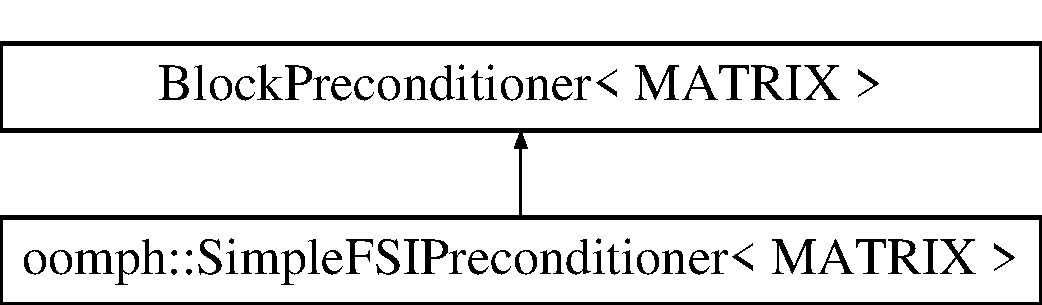
\includegraphics[height=4.000000cm]{classoomph_1_1SimpleFSIPreconditioner}
\end{center}
\end{figure}
\subsection*{Public Member Functions}
\begin{DoxyCompactItemize}
\item 
\hyperlink{classoomph_1_1SimpleFSIPreconditioner_a597c5d3292b1e5e9001f8a738f186a73}{Simple\+F\+S\+I\+Preconditioner} ()
\begin{DoxyCompactList}\small\item\em Constructor. \end{DoxyCompactList}\item 
\hyperlink{classoomph_1_1SimpleFSIPreconditioner_a86515bb32fe8a2cdffda1d185751109d}{$\sim$\+Simple\+F\+S\+I\+Preconditioner} ()
\begin{DoxyCompactList}\small\item\em Destructor\+: Clean up. \end{DoxyCompactList}\item 
\hyperlink{classoomph_1_1SimpleFSIPreconditioner_a427e372b3153e9a26aa97c76d69e28a4}{Simple\+F\+S\+I\+Preconditioner} (const \hyperlink{classoomph_1_1SimpleFSIPreconditioner}{Simple\+F\+S\+I\+Preconditioner} \&)
\begin{DoxyCompactList}\small\item\em Broken copy constructor. \end{DoxyCompactList}\item 
void \hyperlink{classoomph_1_1SimpleFSIPreconditioner_ab9c5875d7186cfb5c55cecb72bed50b3}{set\+\_\+navier\+\_\+stokes\+\_\+mesh} (\hyperlink{classoomph_1_1Mesh}{Mesh} $\ast$\hyperlink{classoomph_1_1BlockPreconditioner_a3c0e92cb77c3e3179007fe9fd99b6428}{mesh\+\_\+pt}, const bool \&allow\+\_\+multiple\+\_\+element\+\_\+type\+\_\+in\+\_\+navier\+\_\+stokes\+\_\+mesh=false)
\begin{DoxyCompactList}\small\item\em Broken assignment operator. \end{DoxyCompactList}\item 
void \hyperlink{classoomph_1_1SimpleFSIPreconditioner_a324b53aaedfc8f0a2cc3da921ef94686}{set\+\_\+wall\+\_\+mesh} (\hyperlink{classoomph_1_1Mesh}{Mesh} $\ast$\hyperlink{classoomph_1_1BlockPreconditioner_a3c0e92cb77c3e3179007fe9fd99b6428}{mesh\+\_\+pt}, const bool \&allow\+\_\+multiple\+\_\+element\+\_\+type\+\_\+in\+\_\+wall\+\_\+mesh=false)
\begin{DoxyCompactList}\small\item\em Setter function for the mesh containing the block-\/preconditionable F\+SI solid elements. \end{DoxyCompactList}\item 
void \hyperlink{classoomph_1_1SimpleFSIPreconditioner_aaf19c0c3f19f6d8ef4f36a1581829230}{setup} ()
\begin{DoxyCompactList}\small\item\em Setup the preconditioner. \end{DoxyCompactList}\item 
void \hyperlink{classoomph_1_1SimpleFSIPreconditioner_a31684c26aa10a782189c32304d9d0824}{preconditioner\+\_\+solve} (const \hyperlink{classoomph_1_1DoubleVector}{Double\+Vector} \&r, \hyperlink{classoomph_1_1DoubleVector}{Double\+Vector} \&z)
\begin{DoxyCompactList}\small\item\em Apply preconditioner to r. \end{DoxyCompactList}\item 
void \hyperlink{classoomph_1_1SimpleFSIPreconditioner_a9e4313b890f586d4e1fb406a1b9d3948}{use\+\_\+block\+\_\+diagonal\+\_\+version} ()
\begin{DoxyCompactList}\small\item\em Switch to block-\/diagonal preconditioner. \end{DoxyCompactList}\item 
void \hyperlink{classoomph_1_1SimpleFSIPreconditioner_ae996d56f6e94d88967e8aad4e664ee74}{use\+\_\+block\+\_\+triangular\+\_\+version\+\_\+with\+\_\+fluid\+\_\+on\+\_\+solid} ()
\begin{DoxyCompactList}\small\item\em Switch to block-\/triangular preconditioner in which action of fluid dofs onto solid equations is retained. \end{DoxyCompactList}\item 
void \hyperlink{classoomph_1_1SimpleFSIPreconditioner_a888de44acd9583fe7cce949a461dfc56}{use\+\_\+block\+\_\+triangular\+\_\+version\+\_\+with\+\_\+solid\+\_\+on\+\_\+fluid} ()
\begin{DoxyCompactList}\small\item\em Switch to block-\/triangular preconditioner in which action of solid dofs onto fluid equations is retained. \end{DoxyCompactList}\end{DoxyCompactItemize}
\subsection*{Private Member Functions}
\begin{DoxyCompactItemize}
\item 
virtual void \hyperlink{classoomph_1_1SimpleFSIPreconditioner_abaf505c05ec128f4c3c6ff5036fb3db1}{identify\+\_\+required\+\_\+blocks} (\hyperlink{classoomph_1_1DenseMatrix}{Dense\+Matrix}$<$ bool $>$ \&required\+\_\+blocks)
\begin{DoxyCompactList}\small\item\em Identify the required blocks\+: Here we only need the momentum, gradient and divergence blocks of the 2x2 block-\/structured fluid matrix, the 1x1 solid block and the selected F\+S\+I-\/off diagonals. \end{DoxyCompactList}\end{DoxyCompactItemize}
\subsection*{Private Attributes}
\begin{DoxyCompactItemize}
\item 
\hyperlink{classoomph_1_1Preconditioner}{Preconditioner} $\ast$ \hyperlink{classoomph_1_1SimpleFSIPreconditioner_aa08cfa51beb62ce3d72f47b8e75ce9f3}{Preconditioner\+\_\+pt}
\begin{DoxyCompactList}\small\item\em \hyperlink{classoomph_1_1Preconditioner}{Preconditioner} (inexact solver) \end{DoxyCompactList}\item 
bool \hyperlink{classoomph_1_1SimpleFSIPreconditioner_a62e9e620ecb6022d20aa09b493f6950d}{Retain\+\_\+solid\+\_\+onto\+\_\+fluid\+\_\+terms}
\begin{DoxyCompactList}\small\item\em Boolean flag used to indicate that the solid onto fluid interaction terms are to be retained. \end{DoxyCompactList}\item 
bool \hyperlink{classoomph_1_1SimpleFSIPreconditioner_a0bc8bfc84237a096d6687d902edcf33b}{Retain\+\_\+fluid\+\_\+onto\+\_\+solid\+\_\+terms}
\begin{DoxyCompactList}\small\item\em Boolean flag used to indicate that the fluid onto solid interaction terms are to be retained. \end{DoxyCompactList}\item 
\hyperlink{classoomph_1_1Mesh}{Mesh} $\ast$ \hyperlink{classoomph_1_1SimpleFSIPreconditioner_a957b57dc5d05df008c15aec8f3c2ea0f}{Navier\+\_\+stokes\+\_\+mesh\+\_\+pt}
\begin{DoxyCompactList}\small\item\em Pointer to the navier stokes mesh. \end{DoxyCompactList}\item 
\hyperlink{classoomph_1_1Mesh}{Mesh} $\ast$ \hyperlink{classoomph_1_1SimpleFSIPreconditioner_a3ad28ce867dc02b67f674ff8e159bff8}{Wall\+\_\+mesh\+\_\+pt}
\begin{DoxyCompactList}\small\item\em pointer to the solid mesh \end{DoxyCompactList}\item 
bool \hyperlink{classoomph_1_1SimpleFSIPreconditioner_a9e1ceded449890704546b3f281bedecb}{Allow\+\_\+multiple\+\_\+element\+\_\+type\+\_\+in\+\_\+navier\+\_\+stokes\+\_\+mesh}
\begin{DoxyCompactList}\small\item\em Flag for multiple element types in the Navier-\/\+Stokes mesh. \end{DoxyCompactList}\item 
bool \hyperlink{classoomph_1_1SimpleFSIPreconditioner_a70094cbfae8c30e11647906cdd7e38c3}{Allow\+\_\+multiple\+\_\+element\+\_\+type\+\_\+in\+\_\+wall\+\_\+mesh}
\begin{DoxyCompactList}\small\item\em Flag for multiple element types in the Wall mesh. \end{DoxyCompactList}\end{DoxyCompactItemize}
\subsection*{Additional Inherited Members}


\subsection{Detailed Description}
\subsubsection*{template$<$typename M\+A\+T\+R\+IX$>$\newline
class oomph\+::\+Simple\+F\+S\+I\+Preconditioner$<$ M\+A\+T\+R\+I\+X $>$}

F\+SI preconditioner. This extracts upper/lower triangular blocks in the 3x3 overall block matrix structure arising from the monolithic discretisation of F\+SI problems with algebraic node updates. Dofs are decomposed into fluid velocity, pressure and solid unknowns. Blocks are then re-\/assembled into one global matrix and solved with a direct solver (Super\+LU in its incarnation as an exact preconditioner). By default we retain the fluid on solid off diagonal blocks. 

Definition at line 499 of file fsi\+\_\+preconditioners.\+h.



\subsection{Constructor \& Destructor Documentation}
\mbox{\Hypertarget{classoomph_1_1SimpleFSIPreconditioner_a597c5d3292b1e5e9001f8a738f186a73}\label{classoomph_1_1SimpleFSIPreconditioner_a597c5d3292b1e5e9001f8a738f186a73}} 
\index{oomph\+::\+Simple\+F\+S\+I\+Preconditioner@{oomph\+::\+Simple\+F\+S\+I\+Preconditioner}!Simple\+F\+S\+I\+Preconditioner@{Simple\+F\+S\+I\+Preconditioner}}
\index{Simple\+F\+S\+I\+Preconditioner@{Simple\+F\+S\+I\+Preconditioner}!oomph\+::\+Simple\+F\+S\+I\+Preconditioner@{oomph\+::\+Simple\+F\+S\+I\+Preconditioner}}
\subsubsection{\texorpdfstring{Simple\+F\+S\+I\+Preconditioner()}{SimpleFSIPreconditioner()}\hspace{0.1cm}{\footnotesize\ttfamily [1/2]}}
{\footnotesize\ttfamily template$<$typename M\+A\+T\+R\+IX $>$ \\
\hyperlink{classoomph_1_1SimpleFSIPreconditioner}{oomph\+::\+Simple\+F\+S\+I\+Preconditioner}$<$ M\+A\+T\+R\+IX $>$\+::\hyperlink{classoomph_1_1SimpleFSIPreconditioner}{Simple\+F\+S\+I\+Preconditioner} (\begin{DoxyParamCaption}{ }\end{DoxyParamCaption})\hspace{0.3cm}{\ttfamily [inline]}}



Constructor. 



Definition at line 505 of file fsi\+\_\+preconditioners.\+h.



References oomph\+::\+F\+S\+I\+Preconditioner\+::\+Allow\+\_\+multiple\+\_\+element\+\_\+type\+\_\+in\+\_\+navier\+\_\+stokes\+\_\+mesh, oomph\+::\+F\+S\+I\+Preconditioner\+::\+Allow\+\_\+multiple\+\_\+element\+\_\+type\+\_\+in\+\_\+wall\+\_\+mesh, oomph\+::\+F\+S\+I\+Preconditioner\+::\+Navier\+\_\+stokes\+\_\+mesh\+\_\+pt, oomph\+::\+F\+S\+I\+Preconditioner\+::\+Retain\+\_\+fluid\+\_\+onto\+\_\+solid\+\_\+terms, oomph\+::\+F\+S\+I\+Preconditioner\+::\+Retain\+\_\+solid\+\_\+onto\+\_\+fluid\+\_\+terms, oomph\+::\+Block\+Preconditioner$<$ C\+R\+Double\+Matrix $>$\+::set\+\_\+nmesh(), and oomph\+::\+F\+S\+I\+Preconditioner\+::\+Wall\+\_\+mesh\+\_\+pt.

\mbox{\Hypertarget{classoomph_1_1SimpleFSIPreconditioner_a86515bb32fe8a2cdffda1d185751109d}\label{classoomph_1_1SimpleFSIPreconditioner_a86515bb32fe8a2cdffda1d185751109d}} 
\index{oomph\+::\+Simple\+F\+S\+I\+Preconditioner@{oomph\+::\+Simple\+F\+S\+I\+Preconditioner}!````~Simple\+F\+S\+I\+Preconditioner@{$\sim$\+Simple\+F\+S\+I\+Preconditioner}}
\index{````~Simple\+F\+S\+I\+Preconditioner@{$\sim$\+Simple\+F\+S\+I\+Preconditioner}!oomph\+::\+Simple\+F\+S\+I\+Preconditioner@{oomph\+::\+Simple\+F\+S\+I\+Preconditioner}}
\subsubsection{\texorpdfstring{$\sim$\+Simple\+F\+S\+I\+Preconditioner()}{~SimpleFSIPreconditioner()}}
{\footnotesize\ttfamily template$<$typename M\+A\+T\+R\+IX $>$ \\
\hyperlink{classoomph_1_1SimpleFSIPreconditioner}{oomph\+::\+Simple\+F\+S\+I\+Preconditioner}$<$ M\+A\+T\+R\+IX $>$\+::$\sim$\hyperlink{classoomph_1_1SimpleFSIPreconditioner}{Simple\+F\+S\+I\+Preconditioner} (\begin{DoxyParamCaption}{ }\end{DoxyParamCaption})\hspace{0.3cm}{\ttfamily [inline]}}



Destructor\+: Clean up. 



Definition at line 527 of file fsi\+\_\+preconditioners.\+h.

\mbox{\Hypertarget{classoomph_1_1SimpleFSIPreconditioner_a427e372b3153e9a26aa97c76d69e28a4}\label{classoomph_1_1SimpleFSIPreconditioner_a427e372b3153e9a26aa97c76d69e28a4}} 
\index{oomph\+::\+Simple\+F\+S\+I\+Preconditioner@{oomph\+::\+Simple\+F\+S\+I\+Preconditioner}!Simple\+F\+S\+I\+Preconditioner@{Simple\+F\+S\+I\+Preconditioner}}
\index{Simple\+F\+S\+I\+Preconditioner@{Simple\+F\+S\+I\+Preconditioner}!oomph\+::\+Simple\+F\+S\+I\+Preconditioner@{oomph\+::\+Simple\+F\+S\+I\+Preconditioner}}
\subsubsection{\texorpdfstring{Simple\+F\+S\+I\+Preconditioner()}{SimpleFSIPreconditioner()}\hspace{0.1cm}{\footnotesize\ttfamily [2/2]}}
{\footnotesize\ttfamily template$<$typename M\+A\+T\+R\+IX $>$ \\
\hyperlink{classoomph_1_1SimpleFSIPreconditioner}{oomph\+::\+Simple\+F\+S\+I\+Preconditioner}$<$ M\+A\+T\+R\+IX $>$\+::\hyperlink{classoomph_1_1SimpleFSIPreconditioner}{Simple\+F\+S\+I\+Preconditioner} (\begin{DoxyParamCaption}\item[{const \hyperlink{classoomph_1_1SimpleFSIPreconditioner}{Simple\+F\+S\+I\+Preconditioner}$<$ M\+A\+T\+R\+IX $>$ \&}]{ }\end{DoxyParamCaption})\hspace{0.3cm}{\ttfamily [inline]}}



Broken copy constructor. 



Definition at line 540 of file fsi\+\_\+preconditioners.\+h.



References oomph\+::\+Broken\+Copy\+::broken\+\_\+copy(), and oomph\+::\+F\+S\+I\+Preconditioner\+::set\+\_\+navier\+\_\+stokes\+\_\+mesh().



\subsection{Member Function Documentation}
\mbox{\Hypertarget{classoomph_1_1SimpleFSIPreconditioner_abaf505c05ec128f4c3c6ff5036fb3db1}\label{classoomph_1_1SimpleFSIPreconditioner_abaf505c05ec128f4c3c6ff5036fb3db1}} 
\index{oomph\+::\+Simple\+F\+S\+I\+Preconditioner@{oomph\+::\+Simple\+F\+S\+I\+Preconditioner}!identify\+\_\+required\+\_\+blocks@{identify\+\_\+required\+\_\+blocks}}
\index{identify\+\_\+required\+\_\+blocks@{identify\+\_\+required\+\_\+blocks}!oomph\+::\+Simple\+F\+S\+I\+Preconditioner@{oomph\+::\+Simple\+F\+S\+I\+Preconditioner}}
\subsubsection{\texorpdfstring{identify\+\_\+required\+\_\+blocks()}{identify\_required\_blocks()}}
{\footnotesize\ttfamily template$<$typename M\+A\+T\+R\+IX $>$ \\
void \hyperlink{classoomph_1_1SimpleFSIPreconditioner}{oomph\+::\+Simple\+F\+S\+I\+Preconditioner}$<$ M\+A\+T\+R\+IX $>$\+::identify\+\_\+required\+\_\+blocks (\begin{DoxyParamCaption}\item[{\hyperlink{classoomph_1_1DenseMatrix}{Dense\+Matrix}$<$ bool $>$ \&}]{required\+\_\+blocks }\end{DoxyParamCaption})\hspace{0.3cm}{\ttfamily [private]}, {\ttfamily [virtual]}}



Identify the required blocks\+: Here we only need the momentum, gradient and divergence blocks of the 2x2 block-\/structured fluid matrix, the 1x1 solid block and the selected F\+S\+I-\/off diagonals. 

Identify the required blocks\+: Here we only need the momentum, gradient and divergence blocks of the 2x2 block-\/structured fluid matrix, the 1x1 solid block and the selected F\+S\+I-\/off diagonals. 

Definition at line 658 of file fsi\+\_\+preconditioners.\+h.



References i, oomph\+::\+Block\+Preconditioner$<$ C\+R\+Double\+Matrix $>$\+::nblock\+\_\+types(), oomph\+::\+F\+S\+I\+Preconditioner\+::\+Retain\+\_\+fluid\+\_\+onto\+\_\+solid\+\_\+terms, oomph\+::\+F\+S\+I\+Preconditioner\+::\+Retain\+\_\+solid\+\_\+onto\+\_\+fluid\+\_\+terms, and oomph\+::\+Simple\+F\+S\+I\+Preconditioner$<$ M\+A\+T\+R\+I\+X $>$\+::setup().

\mbox{\Hypertarget{classoomph_1_1SimpleFSIPreconditioner_a31684c26aa10a782189c32304d9d0824}\label{classoomph_1_1SimpleFSIPreconditioner_a31684c26aa10a782189c32304d9d0824}} 
\index{oomph\+::\+Simple\+F\+S\+I\+Preconditioner@{oomph\+::\+Simple\+F\+S\+I\+Preconditioner}!preconditioner\+\_\+solve@{preconditioner\+\_\+solve}}
\index{preconditioner\+\_\+solve@{preconditioner\+\_\+solve}!oomph\+::\+Simple\+F\+S\+I\+Preconditioner@{oomph\+::\+Simple\+F\+S\+I\+Preconditioner}}
\subsubsection{\texorpdfstring{preconditioner\+\_\+solve()}{preconditioner\_solve()}}
{\footnotesize\ttfamily template$<$typename M\+A\+T\+R\+IX $>$ \\
void \hyperlink{classoomph_1_1SimpleFSIPreconditioner}{oomph\+::\+Simple\+F\+S\+I\+Preconditioner}$<$ M\+A\+T\+R\+IX $>$\+::preconditioner\+\_\+solve (\begin{DoxyParamCaption}\item[{const \hyperlink{classoomph_1_1DoubleVector}{Double\+Vector} \&}]{r,  }\item[{\hyperlink{classoomph_1_1DoubleVector}{Double\+Vector} \&}]{z }\end{DoxyParamCaption})\hspace{0.3cm}{\ttfamily [virtual]}}



Apply preconditioner to r. 

Apply preconditioner to \hyperlink{classoomph_1_1Vector}{Vector} r. 

Implements \hyperlink{classoomph_1_1Preconditioner_ace1199369e4465cd2b9a34884bb64ec8}{oomph\+::\+Preconditioner}.



Definition at line 797 of file fsi\+\_\+preconditioners.\+h.



References oomph\+::\+Block\+Preconditioner$<$ C\+R\+Double\+Matrix $>$\+::get\+\_\+block\+\_\+ordered\+\_\+preconditioner\+\_\+vector(), and oomph\+::\+Block\+Preconditioner$<$ C\+R\+Double\+Matrix $>$\+::return\+\_\+block\+\_\+ordered\+\_\+preconditioner\+\_\+vector().



Referenced by oomph\+::\+Simple\+F\+S\+I\+Preconditioner$<$ M\+A\+T\+R\+I\+X $>$\+::setup().

\mbox{\Hypertarget{classoomph_1_1SimpleFSIPreconditioner_ab9c5875d7186cfb5c55cecb72bed50b3}\label{classoomph_1_1SimpleFSIPreconditioner_ab9c5875d7186cfb5c55cecb72bed50b3}} 
\index{oomph\+::\+Simple\+F\+S\+I\+Preconditioner@{oomph\+::\+Simple\+F\+S\+I\+Preconditioner}!set\+\_\+navier\+\_\+stokes\+\_\+mesh@{set\+\_\+navier\+\_\+stokes\+\_\+mesh}}
\index{set\+\_\+navier\+\_\+stokes\+\_\+mesh@{set\+\_\+navier\+\_\+stokes\+\_\+mesh}!oomph\+::\+Simple\+F\+S\+I\+Preconditioner@{oomph\+::\+Simple\+F\+S\+I\+Preconditioner}}
\subsubsection{\texorpdfstring{set\+\_\+navier\+\_\+stokes\+\_\+mesh()}{set\_navier\_stokes\_mesh()}}
{\footnotesize\ttfamily template$<$typename M\+A\+T\+R\+IX $>$ \\
void \hyperlink{classoomph_1_1SimpleFSIPreconditioner}{oomph\+::\+Simple\+F\+S\+I\+Preconditioner}$<$ M\+A\+T\+R\+IX $>$\+::set\+\_\+navier\+\_\+stokes\+\_\+mesh (\begin{DoxyParamCaption}\item[{\hyperlink{classoomph_1_1Mesh}{Mesh} $\ast$}]{mesh\+\_\+pt,  }\item[{const bool \&}]{allow\+\_\+multiple\+\_\+element\+\_\+type\+\_\+in\+\_\+navier\+\_\+stokes\+\_\+mesh = {\ttfamily false} }\end{DoxyParamCaption})\hspace{0.3cm}{\ttfamily [inline]}}



Broken assignment operator. 

Setter function for the mesh containing the block-\/preconditionable Navier-\/\+Stokes elements. 

Definition at line 555 of file fsi\+\_\+preconditioners.\+h.



References oomph\+::\+F\+S\+I\+Preconditioner\+::\+Allow\+\_\+multiple\+\_\+element\+\_\+type\+\_\+in\+\_\+navier\+\_\+stokes\+\_\+mesh, oomph\+::\+Block\+Preconditioner$<$ C\+R\+Double\+Matrix $>$\+::mesh\+\_\+pt(), oomph\+::\+F\+S\+I\+Preconditioner\+::\+Navier\+\_\+stokes\+\_\+mesh\+\_\+pt, and oomph\+::\+F\+S\+I\+Preconditioner\+::set\+\_\+wall\+\_\+mesh().

\mbox{\Hypertarget{classoomph_1_1SimpleFSIPreconditioner_a324b53aaedfc8f0a2cc3da921ef94686}\label{classoomph_1_1SimpleFSIPreconditioner_a324b53aaedfc8f0a2cc3da921ef94686}} 
\index{oomph\+::\+Simple\+F\+S\+I\+Preconditioner@{oomph\+::\+Simple\+F\+S\+I\+Preconditioner}!set\+\_\+wall\+\_\+mesh@{set\+\_\+wall\+\_\+mesh}}
\index{set\+\_\+wall\+\_\+mesh@{set\+\_\+wall\+\_\+mesh}!oomph\+::\+Simple\+F\+S\+I\+Preconditioner@{oomph\+::\+Simple\+F\+S\+I\+Preconditioner}}
\subsubsection{\texorpdfstring{set\+\_\+wall\+\_\+mesh()}{set\_wall\_mesh()}}
{\footnotesize\ttfamily template$<$typename M\+A\+T\+R\+IX $>$ \\
void \hyperlink{classoomph_1_1SimpleFSIPreconditioner}{oomph\+::\+Simple\+F\+S\+I\+Preconditioner}$<$ M\+A\+T\+R\+IX $>$\+::set\+\_\+wall\+\_\+mesh (\begin{DoxyParamCaption}\item[{\hyperlink{classoomph_1_1Mesh}{Mesh} $\ast$}]{mesh\+\_\+pt,  }\item[{const bool \&}]{allow\+\_\+multiple\+\_\+element\+\_\+type\+\_\+in\+\_\+wall\+\_\+mesh = {\ttfamily false} }\end{DoxyParamCaption})\hspace{0.3cm}{\ttfamily [inline]}}



Setter function for the mesh containing the block-\/preconditionable F\+SI solid elements. 



Definition at line 569 of file fsi\+\_\+preconditioners.\+h.



References oomph\+::\+F\+S\+I\+Preconditioner\+::\+Allow\+\_\+multiple\+\_\+element\+\_\+type\+\_\+in\+\_\+wall\+\_\+mesh, oomph\+::\+Block\+Preconditioner$<$ C\+R\+Double\+Matrix $>$\+::mesh\+\_\+pt(), oomph\+::\+F\+S\+I\+Preconditioner\+::preconditioner\+\_\+solve(), oomph\+::\+F\+S\+I\+Preconditioner\+::setup(), and oomph\+::\+F\+S\+I\+Preconditioner\+::\+Wall\+\_\+mesh\+\_\+pt.

\mbox{\Hypertarget{classoomph_1_1SimpleFSIPreconditioner_aaf19c0c3f19f6d8ef4f36a1581829230}\label{classoomph_1_1SimpleFSIPreconditioner_aaf19c0c3f19f6d8ef4f36a1581829230}} 
\index{oomph\+::\+Simple\+F\+S\+I\+Preconditioner@{oomph\+::\+Simple\+F\+S\+I\+Preconditioner}!setup@{setup}}
\index{setup@{setup}!oomph\+::\+Simple\+F\+S\+I\+Preconditioner@{oomph\+::\+Simple\+F\+S\+I\+Preconditioner}}
\subsubsection{\texorpdfstring{setup()}{setup()}}
{\footnotesize\ttfamily template$<$typename M\+A\+T\+R\+IX $>$ \\
void \hyperlink{classoomph_1_1SimpleFSIPreconditioner}{oomph\+::\+Simple\+F\+S\+I\+Preconditioner}$<$ M\+A\+T\+R\+IX $>$\+::setup (\begin{DoxyParamCaption}{ }\end{DoxyParamCaption})\hspace{0.3cm}{\ttfamily [virtual]}}



Setup the preconditioner. 

Setup the preconditioner\+: Copy the upper/lower triangular block matrices back into a big matrix (with the entries re-\/ordered relative to the original Jacobian matrix). 

Implements \hyperlink{classoomph_1_1Preconditioner_af4886f4efe510e5c9b0eb19422943588}{oomph\+::\+Preconditioner}.



Definition at line 712 of file fsi\+\_\+preconditioners.\+h.



References oomph\+::\+F\+S\+I\+Preconditioner\+::\+Allow\+\_\+multiple\+\_\+element\+\_\+type\+\_\+in\+\_\+navier\+\_\+stokes\+\_\+mesh, oomph\+::\+F\+S\+I\+Preconditioner\+::\+Allow\+\_\+multiple\+\_\+element\+\_\+type\+\_\+in\+\_\+wall\+\_\+mesh, oomph\+::\+Block\+Preconditioner$<$ C\+R\+Double\+Matrix $>$\+::block\+\_\+setup(), oomph\+::\+Block\+Preconditioner$<$ C\+R\+Double\+Matrix $>$\+::get\+\_\+concatenated\+\_\+block(), i, oomph\+::\+F\+S\+I\+Preconditioner\+::\+Navier\+\_\+stokes\+\_\+mesh\+\_\+pt, oomph\+::\+Block\+Preconditioner$<$ C\+R\+Double\+Matrix $>$\+::nblock\+\_\+types(), oomph\+::\+Block\+Preconditioner$<$ C\+R\+Double\+Matrix $>$\+::ndof\+\_\+types\+\_\+in\+\_\+mesh(), oomph\+::\+Simple\+F\+S\+I\+Preconditioner$<$ M\+A\+T\+R\+I\+X $>$\+::preconditioner\+\_\+solve(), oomph\+::\+Block\+Preconditioner$<$ C\+R\+Double\+Matrix $>$\+::set\+\_\+mesh(), oomph\+::\+Super\+L\+U\+Preconditioner\+::setup(), and oomph\+::\+F\+S\+I\+Preconditioner\+::\+Wall\+\_\+mesh\+\_\+pt.



Referenced by oomph\+::\+Simple\+F\+S\+I\+Preconditioner$<$ M\+A\+T\+R\+I\+X $>$\+::identify\+\_\+required\+\_\+blocks().

\mbox{\Hypertarget{classoomph_1_1SimpleFSIPreconditioner_a9e4313b890f586d4e1fb406a1b9d3948}\label{classoomph_1_1SimpleFSIPreconditioner_a9e4313b890f586d4e1fb406a1b9d3948}} 
\index{oomph\+::\+Simple\+F\+S\+I\+Preconditioner@{oomph\+::\+Simple\+F\+S\+I\+Preconditioner}!use\+\_\+block\+\_\+diagonal\+\_\+version@{use\+\_\+block\+\_\+diagonal\+\_\+version}}
\index{use\+\_\+block\+\_\+diagonal\+\_\+version@{use\+\_\+block\+\_\+diagonal\+\_\+version}!oomph\+::\+Simple\+F\+S\+I\+Preconditioner@{oomph\+::\+Simple\+F\+S\+I\+Preconditioner}}
\subsubsection{\texorpdfstring{use\+\_\+block\+\_\+diagonal\+\_\+version()}{use\_block\_diagonal\_version()}}
{\footnotesize\ttfamily template$<$typename M\+A\+T\+R\+IX $>$ \\
void \hyperlink{classoomph_1_1SimpleFSIPreconditioner}{oomph\+::\+Simple\+F\+S\+I\+Preconditioner}$<$ M\+A\+T\+R\+IX $>$\+::use\+\_\+block\+\_\+diagonal\+\_\+version (\begin{DoxyParamCaption}{ }\end{DoxyParamCaption})\hspace{0.3cm}{\ttfamily [inline]}}



Switch to block-\/diagonal preconditioner. 



Definition at line 588 of file fsi\+\_\+preconditioners.\+h.



References oomph\+::\+F\+S\+I\+Preconditioner\+::\+Retain\+\_\+fluid\+\_\+onto\+\_\+solid\+\_\+terms, and oomph\+::\+F\+S\+I\+Preconditioner\+::\+Retain\+\_\+solid\+\_\+onto\+\_\+fluid\+\_\+terms.

\mbox{\Hypertarget{classoomph_1_1SimpleFSIPreconditioner_ae996d56f6e94d88967e8aad4e664ee74}\label{classoomph_1_1SimpleFSIPreconditioner_ae996d56f6e94d88967e8aad4e664ee74}} 
\index{oomph\+::\+Simple\+F\+S\+I\+Preconditioner@{oomph\+::\+Simple\+F\+S\+I\+Preconditioner}!use\+\_\+block\+\_\+triangular\+\_\+version\+\_\+with\+\_\+fluid\+\_\+on\+\_\+solid@{use\+\_\+block\+\_\+triangular\+\_\+version\+\_\+with\+\_\+fluid\+\_\+on\+\_\+solid}}
\index{use\+\_\+block\+\_\+triangular\+\_\+version\+\_\+with\+\_\+fluid\+\_\+on\+\_\+solid@{use\+\_\+block\+\_\+triangular\+\_\+version\+\_\+with\+\_\+fluid\+\_\+on\+\_\+solid}!oomph\+::\+Simple\+F\+S\+I\+Preconditioner@{oomph\+::\+Simple\+F\+S\+I\+Preconditioner}}
\subsubsection{\texorpdfstring{use\+\_\+block\+\_\+triangular\+\_\+version\+\_\+with\+\_\+fluid\+\_\+on\+\_\+solid()}{use\_block\_triangular\_version\_with\_fluid\_on\_solid()}}
{\footnotesize\ttfamily template$<$typename M\+A\+T\+R\+IX $>$ \\
void \hyperlink{classoomph_1_1SimpleFSIPreconditioner}{oomph\+::\+Simple\+F\+S\+I\+Preconditioner}$<$ M\+A\+T\+R\+IX $>$\+::use\+\_\+block\+\_\+triangular\+\_\+version\+\_\+with\+\_\+fluid\+\_\+on\+\_\+solid (\begin{DoxyParamCaption}{ }\end{DoxyParamCaption})\hspace{0.3cm}{\ttfamily [inline]}}



Switch to block-\/triangular preconditioner in which action of fluid dofs onto solid equations is retained. 



Definition at line 596 of file fsi\+\_\+preconditioners.\+h.



References oomph\+::\+F\+S\+I\+Preconditioner\+::\+Retain\+\_\+fluid\+\_\+onto\+\_\+solid\+\_\+terms, and oomph\+::\+F\+S\+I\+Preconditioner\+::\+Retain\+\_\+solid\+\_\+onto\+\_\+fluid\+\_\+terms.

\mbox{\Hypertarget{classoomph_1_1SimpleFSIPreconditioner_a888de44acd9583fe7cce949a461dfc56}\label{classoomph_1_1SimpleFSIPreconditioner_a888de44acd9583fe7cce949a461dfc56}} 
\index{oomph\+::\+Simple\+F\+S\+I\+Preconditioner@{oomph\+::\+Simple\+F\+S\+I\+Preconditioner}!use\+\_\+block\+\_\+triangular\+\_\+version\+\_\+with\+\_\+solid\+\_\+on\+\_\+fluid@{use\+\_\+block\+\_\+triangular\+\_\+version\+\_\+with\+\_\+solid\+\_\+on\+\_\+fluid}}
\index{use\+\_\+block\+\_\+triangular\+\_\+version\+\_\+with\+\_\+solid\+\_\+on\+\_\+fluid@{use\+\_\+block\+\_\+triangular\+\_\+version\+\_\+with\+\_\+solid\+\_\+on\+\_\+fluid}!oomph\+::\+Simple\+F\+S\+I\+Preconditioner@{oomph\+::\+Simple\+F\+S\+I\+Preconditioner}}
\subsubsection{\texorpdfstring{use\+\_\+block\+\_\+triangular\+\_\+version\+\_\+with\+\_\+solid\+\_\+on\+\_\+fluid()}{use\_block\_triangular\_version\_with\_solid\_on\_fluid()}}
{\footnotesize\ttfamily template$<$typename M\+A\+T\+R\+IX $>$ \\
void \hyperlink{classoomph_1_1SimpleFSIPreconditioner}{oomph\+::\+Simple\+F\+S\+I\+Preconditioner}$<$ M\+A\+T\+R\+IX $>$\+::use\+\_\+block\+\_\+triangular\+\_\+version\+\_\+with\+\_\+solid\+\_\+on\+\_\+fluid (\begin{DoxyParamCaption}{ }\end{DoxyParamCaption})\hspace{0.3cm}{\ttfamily [inline]}}



Switch to block-\/triangular preconditioner in which action of solid dofs onto fluid equations is retained. 



Definition at line 604 of file fsi\+\_\+preconditioners.\+h.



References oomph\+::\+F\+S\+I\+Preconditioner\+::\+Retain\+\_\+fluid\+\_\+onto\+\_\+solid\+\_\+terms, and oomph\+::\+F\+S\+I\+Preconditioner\+::\+Retain\+\_\+solid\+\_\+onto\+\_\+fluid\+\_\+terms.



\subsection{Member Data Documentation}
\mbox{\Hypertarget{classoomph_1_1SimpleFSIPreconditioner_a9e1ceded449890704546b3f281bedecb}\label{classoomph_1_1SimpleFSIPreconditioner_a9e1ceded449890704546b3f281bedecb}} 
\index{oomph\+::\+Simple\+F\+S\+I\+Preconditioner@{oomph\+::\+Simple\+F\+S\+I\+Preconditioner}!Allow\+\_\+multiple\+\_\+element\+\_\+type\+\_\+in\+\_\+navier\+\_\+stokes\+\_\+mesh@{Allow\+\_\+multiple\+\_\+element\+\_\+type\+\_\+in\+\_\+navier\+\_\+stokes\+\_\+mesh}}
\index{Allow\+\_\+multiple\+\_\+element\+\_\+type\+\_\+in\+\_\+navier\+\_\+stokes\+\_\+mesh@{Allow\+\_\+multiple\+\_\+element\+\_\+type\+\_\+in\+\_\+navier\+\_\+stokes\+\_\+mesh}!oomph\+::\+Simple\+F\+S\+I\+Preconditioner@{oomph\+::\+Simple\+F\+S\+I\+Preconditioner}}
\subsubsection{\texorpdfstring{Allow\+\_\+multiple\+\_\+element\+\_\+type\+\_\+in\+\_\+navier\+\_\+stokes\+\_\+mesh}{Allow\_multiple\_element\_type\_in\_navier\_stokes\_mesh}}
{\footnotesize\ttfamily template$<$typename M\+A\+T\+R\+IX $>$ \\
bool \hyperlink{classoomph_1_1SimpleFSIPreconditioner}{oomph\+::\+Simple\+F\+S\+I\+Preconditioner}$<$ M\+A\+T\+R\+IX $>$\+::Allow\+\_\+multiple\+\_\+element\+\_\+type\+\_\+in\+\_\+navier\+\_\+stokes\+\_\+mesh\hspace{0.3cm}{\ttfamily [private]}}



Flag for multiple element types in the Navier-\/\+Stokes mesh. 



Definition at line 636 of file fsi\+\_\+preconditioners.\+h.

\mbox{\Hypertarget{classoomph_1_1SimpleFSIPreconditioner_a70094cbfae8c30e11647906cdd7e38c3}\label{classoomph_1_1SimpleFSIPreconditioner_a70094cbfae8c30e11647906cdd7e38c3}} 
\index{oomph\+::\+Simple\+F\+S\+I\+Preconditioner@{oomph\+::\+Simple\+F\+S\+I\+Preconditioner}!Allow\+\_\+multiple\+\_\+element\+\_\+type\+\_\+in\+\_\+wall\+\_\+mesh@{Allow\+\_\+multiple\+\_\+element\+\_\+type\+\_\+in\+\_\+wall\+\_\+mesh}}
\index{Allow\+\_\+multiple\+\_\+element\+\_\+type\+\_\+in\+\_\+wall\+\_\+mesh@{Allow\+\_\+multiple\+\_\+element\+\_\+type\+\_\+in\+\_\+wall\+\_\+mesh}!oomph\+::\+Simple\+F\+S\+I\+Preconditioner@{oomph\+::\+Simple\+F\+S\+I\+Preconditioner}}
\subsubsection{\texorpdfstring{Allow\+\_\+multiple\+\_\+element\+\_\+type\+\_\+in\+\_\+wall\+\_\+mesh}{Allow\_multiple\_element\_type\_in\_wall\_mesh}}
{\footnotesize\ttfamily template$<$typename M\+A\+T\+R\+IX $>$ \\
bool \hyperlink{classoomph_1_1SimpleFSIPreconditioner}{oomph\+::\+Simple\+F\+S\+I\+Preconditioner}$<$ M\+A\+T\+R\+IX $>$\+::Allow\+\_\+multiple\+\_\+element\+\_\+type\+\_\+in\+\_\+wall\+\_\+mesh\hspace{0.3cm}{\ttfamily [private]}}



Flag for multiple element types in the Wall mesh. 



Definition at line 639 of file fsi\+\_\+preconditioners.\+h.

\mbox{\Hypertarget{classoomph_1_1SimpleFSIPreconditioner_a957b57dc5d05df008c15aec8f3c2ea0f}\label{classoomph_1_1SimpleFSIPreconditioner_a957b57dc5d05df008c15aec8f3c2ea0f}} 
\index{oomph\+::\+Simple\+F\+S\+I\+Preconditioner@{oomph\+::\+Simple\+F\+S\+I\+Preconditioner}!Navier\+\_\+stokes\+\_\+mesh\+\_\+pt@{Navier\+\_\+stokes\+\_\+mesh\+\_\+pt}}
\index{Navier\+\_\+stokes\+\_\+mesh\+\_\+pt@{Navier\+\_\+stokes\+\_\+mesh\+\_\+pt}!oomph\+::\+Simple\+F\+S\+I\+Preconditioner@{oomph\+::\+Simple\+F\+S\+I\+Preconditioner}}
\subsubsection{\texorpdfstring{Navier\+\_\+stokes\+\_\+mesh\+\_\+pt}{Navier\_stokes\_mesh\_pt}}
{\footnotesize\ttfamily template$<$typename M\+A\+T\+R\+IX $>$ \\
\hyperlink{classoomph_1_1Mesh}{Mesh}$\ast$ \hyperlink{classoomph_1_1SimpleFSIPreconditioner}{oomph\+::\+Simple\+F\+S\+I\+Preconditioner}$<$ M\+A\+T\+R\+IX $>$\+::Navier\+\_\+stokes\+\_\+mesh\+\_\+pt\hspace{0.3cm}{\ttfamily [private]}}



Pointer to the navier stokes mesh. 



Definition at line 630 of file fsi\+\_\+preconditioners.\+h.

\mbox{\Hypertarget{classoomph_1_1SimpleFSIPreconditioner_aa08cfa51beb62ce3d72f47b8e75ce9f3}\label{classoomph_1_1SimpleFSIPreconditioner_aa08cfa51beb62ce3d72f47b8e75ce9f3}} 
\index{oomph\+::\+Simple\+F\+S\+I\+Preconditioner@{oomph\+::\+Simple\+F\+S\+I\+Preconditioner}!Preconditioner\+\_\+pt@{Preconditioner\+\_\+pt}}
\index{Preconditioner\+\_\+pt@{Preconditioner\+\_\+pt}!oomph\+::\+Simple\+F\+S\+I\+Preconditioner@{oomph\+::\+Simple\+F\+S\+I\+Preconditioner}}
\subsubsection{\texorpdfstring{Preconditioner\+\_\+pt}{Preconditioner\_pt}}
{\footnotesize\ttfamily template$<$typename M\+A\+T\+R\+IX $>$ \\
\hyperlink{classoomph_1_1Preconditioner}{Preconditioner}$\ast$ \hyperlink{classoomph_1_1SimpleFSIPreconditioner}{oomph\+::\+Simple\+F\+S\+I\+Preconditioner}$<$ M\+A\+T\+R\+IX $>$\+::Preconditioner\+\_\+pt\hspace{0.3cm}{\ttfamily [private]}}



\hyperlink{classoomph_1_1Preconditioner}{Preconditioner} (inexact solver) 



Definition at line 613 of file fsi\+\_\+preconditioners.\+h.

\mbox{\Hypertarget{classoomph_1_1SimpleFSIPreconditioner_a0bc8bfc84237a096d6687d902edcf33b}\label{classoomph_1_1SimpleFSIPreconditioner_a0bc8bfc84237a096d6687d902edcf33b}} 
\index{oomph\+::\+Simple\+F\+S\+I\+Preconditioner@{oomph\+::\+Simple\+F\+S\+I\+Preconditioner}!Retain\+\_\+fluid\+\_\+onto\+\_\+solid\+\_\+terms@{Retain\+\_\+fluid\+\_\+onto\+\_\+solid\+\_\+terms}}
\index{Retain\+\_\+fluid\+\_\+onto\+\_\+solid\+\_\+terms@{Retain\+\_\+fluid\+\_\+onto\+\_\+solid\+\_\+terms}!oomph\+::\+Simple\+F\+S\+I\+Preconditioner@{oomph\+::\+Simple\+F\+S\+I\+Preconditioner}}
\subsubsection{\texorpdfstring{Retain\+\_\+fluid\+\_\+onto\+\_\+solid\+\_\+terms}{Retain\_fluid\_onto\_solid\_terms}}
{\footnotesize\ttfamily template$<$typename M\+A\+T\+R\+IX $>$ \\
bool \hyperlink{classoomph_1_1SimpleFSIPreconditioner}{oomph\+::\+Simple\+F\+S\+I\+Preconditioner}$<$ M\+A\+T\+R\+IX $>$\+::Retain\+\_\+fluid\+\_\+onto\+\_\+solid\+\_\+terms\hspace{0.3cm}{\ttfamily [private]}}



Boolean flag used to indicate that the fluid onto solid interaction terms are to be retained. 



Definition at line 621 of file fsi\+\_\+preconditioners.\+h.

\mbox{\Hypertarget{classoomph_1_1SimpleFSIPreconditioner_a62e9e620ecb6022d20aa09b493f6950d}\label{classoomph_1_1SimpleFSIPreconditioner_a62e9e620ecb6022d20aa09b493f6950d}} 
\index{oomph\+::\+Simple\+F\+S\+I\+Preconditioner@{oomph\+::\+Simple\+F\+S\+I\+Preconditioner}!Retain\+\_\+solid\+\_\+onto\+\_\+fluid\+\_\+terms@{Retain\+\_\+solid\+\_\+onto\+\_\+fluid\+\_\+terms}}
\index{Retain\+\_\+solid\+\_\+onto\+\_\+fluid\+\_\+terms@{Retain\+\_\+solid\+\_\+onto\+\_\+fluid\+\_\+terms}!oomph\+::\+Simple\+F\+S\+I\+Preconditioner@{oomph\+::\+Simple\+F\+S\+I\+Preconditioner}}
\subsubsection{\texorpdfstring{Retain\+\_\+solid\+\_\+onto\+\_\+fluid\+\_\+terms}{Retain\_solid\_onto\_fluid\_terms}}
{\footnotesize\ttfamily template$<$typename M\+A\+T\+R\+IX $>$ \\
bool \hyperlink{classoomph_1_1SimpleFSIPreconditioner}{oomph\+::\+Simple\+F\+S\+I\+Preconditioner}$<$ M\+A\+T\+R\+IX $>$\+::Retain\+\_\+solid\+\_\+onto\+\_\+fluid\+\_\+terms\hspace{0.3cm}{\ttfamily [private]}}



Boolean flag used to indicate that the solid onto fluid interaction terms are to be retained. 



Definition at line 617 of file fsi\+\_\+preconditioners.\+h.

\mbox{\Hypertarget{classoomph_1_1SimpleFSIPreconditioner_a3ad28ce867dc02b67f674ff8e159bff8}\label{classoomph_1_1SimpleFSIPreconditioner_a3ad28ce867dc02b67f674ff8e159bff8}} 
\index{oomph\+::\+Simple\+F\+S\+I\+Preconditioner@{oomph\+::\+Simple\+F\+S\+I\+Preconditioner}!Wall\+\_\+mesh\+\_\+pt@{Wall\+\_\+mesh\+\_\+pt}}
\index{Wall\+\_\+mesh\+\_\+pt@{Wall\+\_\+mesh\+\_\+pt}!oomph\+::\+Simple\+F\+S\+I\+Preconditioner@{oomph\+::\+Simple\+F\+S\+I\+Preconditioner}}
\subsubsection{\texorpdfstring{Wall\+\_\+mesh\+\_\+pt}{Wall\_mesh\_pt}}
{\footnotesize\ttfamily template$<$typename M\+A\+T\+R\+IX $>$ \\
\hyperlink{classoomph_1_1Mesh}{Mesh}$\ast$ \hyperlink{classoomph_1_1SimpleFSIPreconditioner}{oomph\+::\+Simple\+F\+S\+I\+Preconditioner}$<$ M\+A\+T\+R\+IX $>$\+::Wall\+\_\+mesh\+\_\+pt\hspace{0.3cm}{\ttfamily [private]}}



pointer to the solid mesh 



Definition at line 633 of file fsi\+\_\+preconditioners.\+h.



The documentation for this class was generated from the following file\+:\begin{DoxyCompactItemize}
\item 
\hyperlink{fsi__preconditioners_8h}{fsi\+\_\+preconditioners.\+h}\end{DoxyCompactItemize}

\hypertarget{classoomph_1_1TimeHarmonicLinElastLoadedByHelmholtzPressureBCElement}{}\section{oomph\+:\+:Time\+Harmonic\+Lin\+Elast\+Loaded\+By\+Helmholtz\+Pressure\+B\+C\+Element$<$ E\+L\+A\+S\+T\+I\+C\+I\+T\+Y\+\_\+\+B\+U\+L\+K\+\_\+\+E\+L\+E\+M\+E\+NT, H\+E\+L\+M\+H\+O\+L\+T\+Z\+\_\+\+B\+U\+L\+K\+\_\+\+E\+L\+E\+M\+E\+NT $>$ Class Template Reference}
\label{classoomph_1_1TimeHarmonicLinElastLoadedByHelmholtzPressureBCElement}\index{oomph\+::\+Time\+Harmonic\+Lin\+Elast\+Loaded\+By\+Helmholtz\+Pressure\+B\+C\+Element$<$ E\+L\+A\+S\+T\+I\+C\+I\+T\+Y\+\_\+\+B\+U\+L\+K\+\_\+\+E\+L\+E\+M\+E\+N\+T, H\+E\+L\+M\+H\+O\+L\+T\+Z\+\_\+\+B\+U\+L\+K\+\_\+\+E\+L\+E\+M\+E\+N\+T $>$@{oomph\+::\+Time\+Harmonic\+Lin\+Elast\+Loaded\+By\+Helmholtz\+Pressure\+B\+C\+Element$<$ E\+L\+A\+S\+T\+I\+C\+I\+T\+Y\+\_\+\+B\+U\+L\+K\+\_\+\+E\+L\+E\+M\+E\+N\+T, H\+E\+L\+M\+H\+O\+L\+T\+Z\+\_\+\+B\+U\+L\+K\+\_\+\+E\+L\+E\+M\+E\+N\+T $>$}}


{\ttfamily \#include $<$helmholtz\+\_\+time\+\_\+harmonic\+\_\+linear\+\_\+elasticity\+\_\+interaction.\+h$>$}

Inheritance diagram for oomph\+:\+:Time\+Harmonic\+Lin\+Elast\+Loaded\+By\+Helmholtz\+Pressure\+B\+C\+Element$<$ E\+L\+A\+S\+T\+I\+C\+I\+T\+Y\+\_\+\+B\+U\+L\+K\+\_\+\+E\+L\+E\+M\+E\+NT, H\+E\+L\+M\+H\+O\+L\+T\+Z\+\_\+\+B\+U\+L\+K\+\_\+\+E\+L\+E\+M\+E\+NT $>$\+:\begin{figure}[H]
\begin{center}
\leavevmode
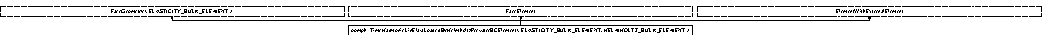
\includegraphics[height=0.562814cm]{classoomph_1_1TimeHarmonicLinElastLoadedByHelmholtzPressureBCElement}
\end{center}
\end{figure}
\subsection*{Public Member Functions}
\begin{DoxyCompactItemize}
\item 
\hyperlink{classoomph_1_1TimeHarmonicLinElastLoadedByHelmholtzPressureBCElement_af0ac460cd2caeb9ba7c7b27e13d5ebc6}{Time\+Harmonic\+Lin\+Elast\+Loaded\+By\+Helmholtz\+Pressure\+B\+C\+Element} (\hyperlink{classoomph_1_1FiniteElement}{Finite\+Element} $\ast$const \&element\+\_\+pt, const int \&\hyperlink{classoomph_1_1FaceElement_a478d577ac6db67ecc80f1f02ae3ab170}{face\+\_\+index})
\begin{DoxyCompactList}\small\item\em Constructor, which takes a \char`\"{}bulk\char`\"{} element and the value of the index and its limit. \end{DoxyCompactList}\item 
void \hyperlink{classoomph_1_1TimeHarmonicLinElastLoadedByHelmholtzPressureBCElement_a0a69b95db2d95da34929a9750d3bce3d}{fill\+\_\+in\+\_\+contribution\+\_\+to\+\_\+residuals} (\hyperlink{classoomph_1_1Vector}{Vector}$<$ double $>$ \&residuals)
\begin{DoxyCompactList}\small\item\em Return the residuals. \end{DoxyCompactList}\item 
void \hyperlink{classoomph_1_1TimeHarmonicLinElastLoadedByHelmholtzPressureBCElement_a151fa0b3aa8df4a582d62d82ae42f40e}{fill\+\_\+in\+\_\+contribution\+\_\+to\+\_\+jacobian} (\hyperlink{classoomph_1_1Vector}{Vector}$<$ double $>$ \&residuals, \hyperlink{classoomph_1_1DenseMatrix}{Dense\+Matrix}$<$ double $>$ \&jacobian)
\begin{DoxyCompactList}\small\item\em Fill in contribution from Jacobian. \end{DoxyCompactList}\item 
const double \& \hyperlink{classoomph_1_1TimeHarmonicLinElastLoadedByHelmholtzPressureBCElement_af8f267ad94739fefd852796732eea1bd}{q} () const
\begin{DoxyCompactList}\small\item\em Return the ratio of the stress scales used to non-\/dimensionalise the fluid and elasticity equations. E.\+g. $ Q = (\omega a)^2 \rho/E $, i.\+e. the ratio between the inertial fluid stress and the solid\textquotesingle{}s elastic modulus E. \end{DoxyCompactList}\item 
double $\ast$\& \hyperlink{classoomph_1_1TimeHarmonicLinElastLoadedByHelmholtzPressureBCElement_a2b836c57f104d02c934615333f306a21}{q\+\_\+pt} ()
\begin{DoxyCompactList}\small\item\em Return a pointer the ratio of stress scales used to non-\/dimensionalise the fluid and solid equations. \end{DoxyCompactList}\item 
void \hyperlink{classoomph_1_1TimeHarmonicLinElastLoadedByHelmholtzPressureBCElement_a1ecf56e825d5af950572efe4208ad307}{output} (std\+::ostream \&outfile)
\begin{DoxyCompactList}\small\item\em Output function. \end{DoxyCompactList}\item 
void \hyperlink{classoomph_1_1TimeHarmonicLinElastLoadedByHelmholtzPressureBCElement_a2cfc5c6af366019bc8d8d9bb42ffae03}{output} (std\+::ostream \&outfile, const unsigned \&n\+\_\+plot)
\begin{DoxyCompactList}\small\item\em Output function\+: Plot traction etc at \hyperlink{classoomph_1_1Gauss}{Gauss} points nplot is ignored. \end{DoxyCompactList}\item 
void \hyperlink{classoomph_1_1TimeHarmonicLinElastLoadedByHelmholtzPressureBCElement_a6a1d8e8ae161b0ca0aa3de8d2a04a409}{output} (F\+I\+LE $\ast$file\+\_\+pt)
\begin{DoxyCompactList}\small\item\em C\+\_\+style output function. \end{DoxyCompactList}\item 
void \hyperlink{classoomph_1_1TimeHarmonicLinElastLoadedByHelmholtzPressureBCElement_aab8bf1e29247d96cef5a0ab8c593de61}{output} (F\+I\+LE $\ast$file\+\_\+pt, const unsigned \&n\+\_\+plot)
\begin{DoxyCompactList}\small\item\em C-\/style output function. \end{DoxyCompactList}\end{DoxyCompactItemize}
\subsection*{Protected Member Functions}
\begin{DoxyCompactItemize}
\item 
void \hyperlink{classoomph_1_1TimeHarmonicLinElastLoadedByHelmholtzPressureBCElement_a42333cd2a19c901bc01d666d85a4e108}{fill\+\_\+in\+\_\+contribution\+\_\+to\+\_\+residuals\+\_\+helmholtz\+\_\+traction} (\hyperlink{classoomph_1_1Vector}{Vector}$<$ double $>$ \&residuals)
\begin{DoxyCompactList}\small\item\em Helper function that actually calculates the residuals. \end{DoxyCompactList}\end{DoxyCompactItemize}
\subsection*{Protected Attributes}
\begin{DoxyCompactItemize}
\item 
double $\ast$ \hyperlink{classoomph_1_1TimeHarmonicLinElastLoadedByHelmholtzPressureBCElement_ae5d333e308981db0bd733cbaa139a538}{Q\+\_\+pt}
\begin{DoxyCompactList}\small\item\em Pointer to the ratio, $ Q $ , of the stress used to non-\/dimensionalise the fluid stresses to the stress used to non-\/dimensionalise the solid stresses. \end{DoxyCompactList}\item 
\hyperlink{classoomph_1_1Vector}{Vector}$<$ std\+::complex$<$ unsigned $>$ $>$ \hyperlink{classoomph_1_1TimeHarmonicLinElastLoadedByHelmholtzPressureBCElement_a65d16036ca5c85f6cf501a992f6e85df}{U\+\_\+index\+\_\+time\+\_\+harmonic\+\_\+linear\+\_\+elasticity\+\_\+helmholtz\+\_\+traction}
\begin{DoxyCompactList}\small\item\em Index at which the i-\/th displacement component is stored. \end{DoxyCompactList}\end{DoxyCompactItemize}
\subsection*{Static Protected Attributes}
\begin{DoxyCompactItemize}
\item 
static double \hyperlink{classoomph_1_1TimeHarmonicLinElastLoadedByHelmholtzPressureBCElement_a71a4d2fe30c7423a08c883843fec938b}{Default\+\_\+\+Q\+\_\+\+Value} =1.\+0
\begin{DoxyCompactList}\small\item\em Static default value for the ratio of stress scales used in the fluid and solid equations (default is 1.\+0) \end{DoxyCompactList}\end{DoxyCompactItemize}
\subsection*{Additional Inherited Members}


\subsection{Detailed Description}
\subsubsection*{template$<$class E\+L\+A\+S\+T\+I\+C\+I\+T\+Y\+\_\+\+B\+U\+L\+K\+\_\+\+E\+L\+E\+M\+E\+NT, class H\+E\+L\+M\+H\+O\+L\+T\+Z\+\_\+\+B\+U\+L\+K\+\_\+\+E\+L\+E\+M\+E\+NT$>$\newline
class oomph\+::\+Time\+Harmonic\+Lin\+Elast\+Loaded\+By\+Helmholtz\+Pressure\+B\+C\+Element$<$ E\+L\+A\+S\+T\+I\+C\+I\+T\+Y\+\_\+\+B\+U\+L\+K\+\_\+\+E\+L\+E\+M\+E\+N\+T, H\+E\+L\+M\+H\+O\+L\+T\+Z\+\_\+\+B\+U\+L\+K\+\_\+\+E\+L\+E\+M\+E\+N\+T $>$}

A class for elements that allow the imposition of an applied traction in the equations of time-\/harmonic linear elasticity from a Helmholtz potential (interpreted as a displacement potential for the fluid in a quasi-\/steady, linearised F\+SI problem.) The geometrical information can be read from the Face\+Geometry$<$\+E\+L\+E\+M\+E\+N\+T$>$ class and and thus, we can be generic enough without the need to have a separate equations class. 

Definition at line 51 of file helmholtz\+\_\+time\+\_\+harmonic\+\_\+linear\+\_\+elasticity\+\_\+interaction.\+h.



\subsection{Constructor \& Destructor Documentation}
\mbox{\Hypertarget{classoomph_1_1TimeHarmonicLinElastLoadedByHelmholtzPressureBCElement_af0ac460cd2caeb9ba7c7b27e13d5ebc6}\label{classoomph_1_1TimeHarmonicLinElastLoadedByHelmholtzPressureBCElement_af0ac460cd2caeb9ba7c7b27e13d5ebc6}} 
\index{oomph\+::\+Time\+Harmonic\+Lin\+Elast\+Loaded\+By\+Helmholtz\+Pressure\+B\+C\+Element@{oomph\+::\+Time\+Harmonic\+Lin\+Elast\+Loaded\+By\+Helmholtz\+Pressure\+B\+C\+Element}!Time\+Harmonic\+Lin\+Elast\+Loaded\+By\+Helmholtz\+Pressure\+B\+C\+Element@{Time\+Harmonic\+Lin\+Elast\+Loaded\+By\+Helmholtz\+Pressure\+B\+C\+Element}}
\index{Time\+Harmonic\+Lin\+Elast\+Loaded\+By\+Helmholtz\+Pressure\+B\+C\+Element@{Time\+Harmonic\+Lin\+Elast\+Loaded\+By\+Helmholtz\+Pressure\+B\+C\+Element}!oomph\+::\+Time\+Harmonic\+Lin\+Elast\+Loaded\+By\+Helmholtz\+Pressure\+B\+C\+Element@{oomph\+::\+Time\+Harmonic\+Lin\+Elast\+Loaded\+By\+Helmholtz\+Pressure\+B\+C\+Element}}
\subsubsection{\texorpdfstring{Time\+Harmonic\+Lin\+Elast\+Loaded\+By\+Helmholtz\+Pressure\+B\+C\+Element()}{TimeHarmonicLinElastLoadedByHelmholtzPressureBCElement()}}
{\footnotesize\ttfamily template$<$class E\+L\+A\+S\+T\+I\+C\+I\+T\+Y\+\_\+\+B\+U\+L\+K\+\_\+\+E\+L\+E\+M\+E\+NT , class H\+E\+L\+M\+H\+O\+L\+T\+Z\+\_\+\+B\+U\+L\+K\+\_\+\+E\+L\+E\+M\+E\+NT $>$ \\
\hyperlink{classoomph_1_1TimeHarmonicLinElastLoadedByHelmholtzPressureBCElement}{oomph\+::\+Time\+Harmonic\+Lin\+Elast\+Loaded\+By\+Helmholtz\+Pressure\+B\+C\+Element}$<$ E\+L\+A\+S\+T\+I\+C\+I\+T\+Y\+\_\+\+B\+U\+L\+K\+\_\+\+E\+L\+E\+M\+E\+NT, H\+E\+L\+M\+H\+O\+L\+T\+Z\+\_\+\+B\+U\+L\+K\+\_\+\+E\+L\+E\+M\+E\+NT $>$\+::\hyperlink{classoomph_1_1TimeHarmonicLinElastLoadedByHelmholtzPressureBCElement}{Time\+Harmonic\+Lin\+Elast\+Loaded\+By\+Helmholtz\+Pressure\+B\+C\+Element} (\begin{DoxyParamCaption}\item[{\hyperlink{classoomph_1_1FiniteElement}{Finite\+Element} $\ast$const \&}]{element\+\_\+pt,  }\item[{const int \&}]{face\+\_\+index }\end{DoxyParamCaption})\hspace{0.3cm}{\ttfamily [inline]}}



Constructor, which takes a \char`\"{}bulk\char`\"{} element and the value of the index and its limit. 



Definition at line 83 of file helmholtz\+\_\+time\+\_\+harmonic\+\_\+linear\+\_\+elasticity\+\_\+interaction.\+h.



References oomph\+::\+Finite\+Element\+::build\+\_\+face\+\_\+element(), oomph\+::\+Finite\+Element\+::has\+\_\+hanging\+\_\+nodes(), i, oomph\+::\+Finite\+Element\+::nodal\+\_\+dimension(), oomph\+::\+Element\+With\+External\+Element\+::set\+\_\+ninteraction(), and oomph\+::\+Time\+Harmonic\+Lin\+Elast\+Loaded\+By\+Helmholtz\+Pressure\+B\+C\+Element$<$ E\+L\+A\+S\+T\+I\+C\+I\+T\+Y\+\_\+\+B\+U\+L\+K\+\_\+\+E\+L\+E\+M\+E\+N\+T, H\+E\+L\+M\+H\+O\+L\+T\+Z\+\_\+\+B\+U\+L\+K\+\_\+\+E\+L\+E\+M\+E\+N\+T $>$\+::\+U\+\_\+index\+\_\+time\+\_\+harmonic\+\_\+linear\+\_\+elasticity\+\_\+helmholtz\+\_\+traction.



\subsection{Member Function Documentation}
\mbox{\Hypertarget{classoomph_1_1TimeHarmonicLinElastLoadedByHelmholtzPressureBCElement_a151fa0b3aa8df4a582d62d82ae42f40e}\label{classoomph_1_1TimeHarmonicLinElastLoadedByHelmholtzPressureBCElement_a151fa0b3aa8df4a582d62d82ae42f40e}} 
\index{oomph\+::\+Time\+Harmonic\+Lin\+Elast\+Loaded\+By\+Helmholtz\+Pressure\+B\+C\+Element@{oomph\+::\+Time\+Harmonic\+Lin\+Elast\+Loaded\+By\+Helmholtz\+Pressure\+B\+C\+Element}!fill\+\_\+in\+\_\+contribution\+\_\+to\+\_\+jacobian@{fill\+\_\+in\+\_\+contribution\+\_\+to\+\_\+jacobian}}
\index{fill\+\_\+in\+\_\+contribution\+\_\+to\+\_\+jacobian@{fill\+\_\+in\+\_\+contribution\+\_\+to\+\_\+jacobian}!oomph\+::\+Time\+Harmonic\+Lin\+Elast\+Loaded\+By\+Helmholtz\+Pressure\+B\+C\+Element@{oomph\+::\+Time\+Harmonic\+Lin\+Elast\+Loaded\+By\+Helmholtz\+Pressure\+B\+C\+Element}}
\subsubsection{\texorpdfstring{fill\+\_\+in\+\_\+contribution\+\_\+to\+\_\+jacobian()}{fill\_in\_contribution\_to\_jacobian()}}
{\footnotesize\ttfamily template$<$class E\+L\+A\+S\+T\+I\+C\+I\+T\+Y\+\_\+\+B\+U\+L\+K\+\_\+\+E\+L\+E\+M\+E\+NT , class H\+E\+L\+M\+H\+O\+L\+T\+Z\+\_\+\+B\+U\+L\+K\+\_\+\+E\+L\+E\+M\+E\+NT $>$ \\
void \hyperlink{classoomph_1_1TimeHarmonicLinElastLoadedByHelmholtzPressureBCElement}{oomph\+::\+Time\+Harmonic\+Lin\+Elast\+Loaded\+By\+Helmholtz\+Pressure\+B\+C\+Element}$<$ E\+L\+A\+S\+T\+I\+C\+I\+T\+Y\+\_\+\+B\+U\+L\+K\+\_\+\+E\+L\+E\+M\+E\+NT, H\+E\+L\+M\+H\+O\+L\+T\+Z\+\_\+\+B\+U\+L\+K\+\_\+\+E\+L\+E\+M\+E\+NT $>$\+::fill\+\_\+in\+\_\+contribution\+\_\+to\+\_\+jacobian (\begin{DoxyParamCaption}\item[{\hyperlink{classoomph_1_1Vector}{Vector}$<$ double $>$ \&}]{residuals,  }\item[{\hyperlink{classoomph_1_1DenseMatrix}{Dense\+Matrix}$<$ double $>$ \&}]{jacobian }\end{DoxyParamCaption})\hspace{0.3cm}{\ttfamily [inline]}, {\ttfamily [virtual]}}



Fill in contribution from Jacobian. 



Reimplemented from \hyperlink{classoomph_1_1ElementWithExternalElement_ae5fb09552a8271e891438f8d058ca1b8}{oomph\+::\+Element\+With\+External\+Element}.



Definition at line 147 of file helmholtz\+\_\+time\+\_\+harmonic\+\_\+linear\+\_\+elasticity\+\_\+interaction.\+h.



References oomph\+::\+Time\+Harmonic\+Lin\+Elast\+Loaded\+By\+Helmholtz\+Pressure\+B\+C\+Element$<$ E\+L\+A\+S\+T\+I\+C\+I\+T\+Y\+\_\+\+B\+U\+L\+K\+\_\+\+E\+L\+E\+M\+E\+N\+T, H\+E\+L\+M\+H\+O\+L\+T\+Z\+\_\+\+B\+U\+L\+K\+\_\+\+E\+L\+E\+M\+E\+N\+T $>$\+::fill\+\_\+in\+\_\+contribution\+\_\+to\+\_\+residuals\+\_\+helmholtz\+\_\+traction(), and oomph\+::\+Element\+With\+External\+Element\+::fill\+\_\+in\+\_\+jacobian\+\_\+from\+\_\+external\+\_\+interaction\+\_\+by\+\_\+fd().

\mbox{\Hypertarget{classoomph_1_1TimeHarmonicLinElastLoadedByHelmholtzPressureBCElement_a0a69b95db2d95da34929a9750d3bce3d}\label{classoomph_1_1TimeHarmonicLinElastLoadedByHelmholtzPressureBCElement_a0a69b95db2d95da34929a9750d3bce3d}} 
\index{oomph\+::\+Time\+Harmonic\+Lin\+Elast\+Loaded\+By\+Helmholtz\+Pressure\+B\+C\+Element@{oomph\+::\+Time\+Harmonic\+Lin\+Elast\+Loaded\+By\+Helmholtz\+Pressure\+B\+C\+Element}!fill\+\_\+in\+\_\+contribution\+\_\+to\+\_\+residuals@{fill\+\_\+in\+\_\+contribution\+\_\+to\+\_\+residuals}}
\index{fill\+\_\+in\+\_\+contribution\+\_\+to\+\_\+residuals@{fill\+\_\+in\+\_\+contribution\+\_\+to\+\_\+residuals}!oomph\+::\+Time\+Harmonic\+Lin\+Elast\+Loaded\+By\+Helmholtz\+Pressure\+B\+C\+Element@{oomph\+::\+Time\+Harmonic\+Lin\+Elast\+Loaded\+By\+Helmholtz\+Pressure\+B\+C\+Element}}
\subsubsection{\texorpdfstring{fill\+\_\+in\+\_\+contribution\+\_\+to\+\_\+residuals()}{fill\_in\_contribution\_to\_residuals()}}
{\footnotesize\ttfamily template$<$class E\+L\+A\+S\+T\+I\+C\+I\+T\+Y\+\_\+\+B\+U\+L\+K\+\_\+\+E\+L\+E\+M\+E\+NT , class H\+E\+L\+M\+H\+O\+L\+T\+Z\+\_\+\+B\+U\+L\+K\+\_\+\+E\+L\+E\+M\+E\+NT $>$ \\
void \hyperlink{classoomph_1_1TimeHarmonicLinElastLoadedByHelmholtzPressureBCElement}{oomph\+::\+Time\+Harmonic\+Lin\+Elast\+Loaded\+By\+Helmholtz\+Pressure\+B\+C\+Element}$<$ E\+L\+A\+S\+T\+I\+C\+I\+T\+Y\+\_\+\+B\+U\+L\+K\+\_\+\+E\+L\+E\+M\+E\+NT, H\+E\+L\+M\+H\+O\+L\+T\+Z\+\_\+\+B\+U\+L\+K\+\_\+\+E\+L\+E\+M\+E\+NT $>$\+::fill\+\_\+in\+\_\+contribution\+\_\+to\+\_\+residuals (\begin{DoxyParamCaption}\item[{\hyperlink{classoomph_1_1Vector}{Vector}$<$ double $>$ \&}]{residuals }\end{DoxyParamCaption})\hspace{0.3cm}{\ttfamily [inline]}, {\ttfamily [virtual]}}



Return the residuals. 



Reimplemented from \hyperlink{classoomph_1_1GeneralisedElement_a310c97f515e8504a48179c0e72c550d7}{oomph\+::\+Generalised\+Element}.



Definition at line 139 of file helmholtz\+\_\+time\+\_\+harmonic\+\_\+linear\+\_\+elasticity\+\_\+interaction.\+h.



References oomph\+::\+Time\+Harmonic\+Lin\+Elast\+Loaded\+By\+Helmholtz\+Pressure\+B\+C\+Element$<$ E\+L\+A\+S\+T\+I\+C\+I\+T\+Y\+\_\+\+B\+U\+L\+K\+\_\+\+E\+L\+E\+M\+E\+N\+T, H\+E\+L\+M\+H\+O\+L\+T\+Z\+\_\+\+B\+U\+L\+K\+\_\+\+E\+L\+E\+M\+E\+N\+T $>$\+::fill\+\_\+in\+\_\+contribution\+\_\+to\+\_\+residuals\+\_\+helmholtz\+\_\+traction().

\mbox{\Hypertarget{classoomph_1_1TimeHarmonicLinElastLoadedByHelmholtzPressureBCElement_a42333cd2a19c901bc01d666d85a4e108}\label{classoomph_1_1TimeHarmonicLinElastLoadedByHelmholtzPressureBCElement_a42333cd2a19c901bc01d666d85a4e108}} 
\index{oomph\+::\+Time\+Harmonic\+Lin\+Elast\+Loaded\+By\+Helmholtz\+Pressure\+B\+C\+Element@{oomph\+::\+Time\+Harmonic\+Lin\+Elast\+Loaded\+By\+Helmholtz\+Pressure\+B\+C\+Element}!fill\+\_\+in\+\_\+contribution\+\_\+to\+\_\+residuals\+\_\+helmholtz\+\_\+traction@{fill\+\_\+in\+\_\+contribution\+\_\+to\+\_\+residuals\+\_\+helmholtz\+\_\+traction}}
\index{fill\+\_\+in\+\_\+contribution\+\_\+to\+\_\+residuals\+\_\+helmholtz\+\_\+traction@{fill\+\_\+in\+\_\+contribution\+\_\+to\+\_\+residuals\+\_\+helmholtz\+\_\+traction}!oomph\+::\+Time\+Harmonic\+Lin\+Elast\+Loaded\+By\+Helmholtz\+Pressure\+B\+C\+Element@{oomph\+::\+Time\+Harmonic\+Lin\+Elast\+Loaded\+By\+Helmholtz\+Pressure\+B\+C\+Element}}
\subsubsection{\texorpdfstring{fill\+\_\+in\+\_\+contribution\+\_\+to\+\_\+residuals\+\_\+helmholtz\+\_\+traction()}{fill\_in\_contribution\_to\_residuals\_helmholtz\_traction()}}
{\footnotesize\ttfamily template$<$class E\+L\+A\+S\+T\+I\+C\+I\+T\+Y\+\_\+\+B\+U\+L\+K\+\_\+\+E\+L\+E\+M\+E\+NT , class H\+E\+L\+M\+H\+O\+L\+T\+Z\+\_\+\+B\+U\+L\+K\+\_\+\+E\+L\+E\+M\+E\+NT $>$ \\
void \hyperlink{classoomph_1_1TimeHarmonicLinElastLoadedByHelmholtzPressureBCElement}{oomph\+::\+Time\+Harmonic\+Lin\+Elast\+Loaded\+By\+Helmholtz\+Pressure\+B\+C\+Element}$<$ E\+L\+A\+S\+T\+I\+C\+I\+T\+Y\+\_\+\+B\+U\+L\+K\+\_\+\+E\+L\+E\+M\+E\+NT, H\+E\+L\+M\+H\+O\+L\+T\+Z\+\_\+\+B\+U\+L\+K\+\_\+\+E\+L\+E\+M\+E\+NT $>$\+::fill\+\_\+in\+\_\+contribution\+\_\+to\+\_\+residuals\+\_\+helmholtz\+\_\+traction (\begin{DoxyParamCaption}\item[{\hyperlink{classoomph_1_1Vector}{Vector}$<$ double $>$ \&}]{residuals }\end{DoxyParamCaption})\hspace{0.3cm}{\ttfamily [protected]}}



Helper function that actually calculates the residuals. 

Return the residuals. 

Definition at line 276 of file helmholtz\+\_\+time\+\_\+harmonic\+\_\+linear\+\_\+elasticity\+\_\+interaction.\+h.



References oomph\+::\+Finite\+Element\+::dshape\+\_\+local\+\_\+at\+\_\+knot(), oomph\+::\+Element\+With\+External\+Element\+::external\+\_\+element\+\_\+local\+\_\+coord(), oomph\+::\+Element\+With\+External\+Element\+::external\+\_\+element\+\_\+pt(), i, oomph\+::\+Finite\+Element\+::integral\+\_\+pt(), oomph\+::\+Face\+Element\+::interpolated\+\_\+x(), oomph\+::\+Finite\+Element\+::nnodal\+\_\+position\+\_\+type(), oomph\+::\+Finite\+Element\+::nnode(), oomph\+::\+Finite\+Element\+::nodal\+\_\+dimension(), oomph\+::\+Finite\+Element\+::nodal\+\_\+local\+\_\+eqn(), oomph\+::\+Finite\+Element\+::nodal\+\_\+position(), oomph\+::\+Integral\+::nweight(), oomph\+::\+Face\+Element\+::outer\+\_\+unit\+\_\+normal(), oomph\+::\+Time\+Harmonic\+Lin\+Elast\+Loaded\+By\+Helmholtz\+Pressure\+B\+C\+Element$<$ E\+L\+A\+S\+T\+I\+C\+I\+T\+Y\+\_\+\+B\+U\+L\+K\+\_\+\+E\+L\+E\+M\+E\+N\+T, H\+E\+L\+M\+H\+O\+L\+T\+Z\+\_\+\+B\+U\+L\+K\+\_\+\+E\+L\+E\+M\+E\+N\+T $>$\+::q(), oomph\+::\+Time\+Harmonic\+Lin\+Elast\+Loaded\+By\+Helmholtz\+Pressure\+B\+C\+Element$<$ E\+L\+A\+S\+T\+I\+C\+I\+T\+Y\+\_\+\+B\+U\+L\+K\+\_\+\+E\+L\+E\+M\+E\+N\+T, H\+E\+L\+M\+H\+O\+L\+T\+Z\+\_\+\+B\+U\+L\+K\+\_\+\+E\+L\+E\+M\+E\+N\+T $>$\+::\+U\+\_\+index\+\_\+time\+\_\+harmonic\+\_\+linear\+\_\+elasticity\+\_\+helmholtz\+\_\+traction, oomph\+::\+Quad\+Tree\+Names\+::W, and oomph\+::\+Integral\+::weight().



Referenced by oomph\+::\+Time\+Harmonic\+Lin\+Elast\+Loaded\+By\+Helmholtz\+Pressure\+B\+C\+Element$<$ E\+L\+A\+S\+T\+I\+C\+I\+T\+Y\+\_\+\+B\+U\+L\+K\+\_\+\+E\+L\+E\+M\+E\+N\+T, H\+E\+L\+M\+H\+O\+L\+T\+Z\+\_\+\+B\+U\+L\+K\+\_\+\+E\+L\+E\+M\+E\+N\+T $>$\+::fill\+\_\+in\+\_\+contribution\+\_\+to\+\_\+jacobian(), oomph\+::\+Time\+Harmonic\+Lin\+Elast\+Loaded\+By\+Helmholtz\+Pressure\+B\+C\+Element$<$ E\+L\+A\+S\+T\+I\+C\+I\+T\+Y\+\_\+\+B\+U\+L\+K\+\_\+\+E\+L\+E\+M\+E\+N\+T, H\+E\+L\+M\+H\+O\+L\+T\+Z\+\_\+\+B\+U\+L\+K\+\_\+\+E\+L\+E\+M\+E\+N\+T $>$\+::fill\+\_\+in\+\_\+contribution\+\_\+to\+\_\+residuals(), and oomph\+::\+Time\+Harmonic\+Lin\+Elast\+Loaded\+By\+Helmholtz\+Pressure\+B\+C\+Element$<$ E\+L\+A\+S\+T\+I\+C\+I\+T\+Y\+\_\+\+B\+U\+L\+K\+\_\+\+E\+L\+E\+M\+E\+N\+T, H\+E\+L\+M\+H\+O\+L\+T\+Z\+\_\+\+B\+U\+L\+K\+\_\+\+E\+L\+E\+M\+E\+N\+T $>$\+::output().

\mbox{\Hypertarget{classoomph_1_1TimeHarmonicLinElastLoadedByHelmholtzPressureBCElement_a1ecf56e825d5af950572efe4208ad307}\label{classoomph_1_1TimeHarmonicLinElastLoadedByHelmholtzPressureBCElement_a1ecf56e825d5af950572efe4208ad307}} 
\index{oomph\+::\+Time\+Harmonic\+Lin\+Elast\+Loaded\+By\+Helmholtz\+Pressure\+B\+C\+Element@{oomph\+::\+Time\+Harmonic\+Lin\+Elast\+Loaded\+By\+Helmholtz\+Pressure\+B\+C\+Element}!output@{output}}
\index{output@{output}!oomph\+::\+Time\+Harmonic\+Lin\+Elast\+Loaded\+By\+Helmholtz\+Pressure\+B\+C\+Element@{oomph\+::\+Time\+Harmonic\+Lin\+Elast\+Loaded\+By\+Helmholtz\+Pressure\+B\+C\+Element}}
\subsubsection{\texorpdfstring{output()}{output()}\hspace{0.1cm}{\footnotesize\ttfamily [1/4]}}
{\footnotesize\ttfamily template$<$class E\+L\+A\+S\+T\+I\+C\+I\+T\+Y\+\_\+\+B\+U\+L\+K\+\_\+\+E\+L\+E\+M\+E\+NT , class H\+E\+L\+M\+H\+O\+L\+T\+Z\+\_\+\+B\+U\+L\+K\+\_\+\+E\+L\+E\+M\+E\+NT $>$ \\
void \hyperlink{classoomph_1_1TimeHarmonicLinElastLoadedByHelmholtzPressureBCElement}{oomph\+::\+Time\+Harmonic\+Lin\+Elast\+Loaded\+By\+Helmholtz\+Pressure\+B\+C\+Element}$<$ E\+L\+A\+S\+T\+I\+C\+I\+T\+Y\+\_\+\+B\+U\+L\+K\+\_\+\+E\+L\+E\+M\+E\+NT, H\+E\+L\+M\+H\+O\+L\+T\+Z\+\_\+\+B\+U\+L\+K\+\_\+\+E\+L\+E\+M\+E\+NT $>$\+::output (\begin{DoxyParamCaption}\item[{std\+::ostream \&}]{outfile }\end{DoxyParamCaption})\hspace{0.3cm}{\ttfamily [inline]}, {\ttfamily [virtual]}}



Output function. 

Dummy 

Reimplemented from \hyperlink{classoomph_1_1FiniteElement_a2ad98a3d2ef4999f1bef62c0ff13f2a7}{oomph\+::\+Finite\+Element}.



Definition at line 170 of file helmholtz\+\_\+time\+\_\+harmonic\+\_\+linear\+\_\+elasticity\+\_\+interaction.\+h.



Referenced by oomph\+::\+Helmholtz\+Flux\+From\+Normal\+Displacement\+B\+C\+Element$<$ H\+E\+L\+M\+H\+O\+L\+T\+Z\+\_\+\+B\+U\+L\+K\+\_\+\+E\+L\+E\+M\+E\+N\+T, E\+L\+A\+S\+T\+I\+C\+I\+T\+Y\+\_\+\+B\+U\+L\+K\+\_\+\+E\+L\+E\+M\+E\+N\+T $>$\+::output().

\mbox{\Hypertarget{classoomph_1_1TimeHarmonicLinElastLoadedByHelmholtzPressureBCElement_a2cfc5c6af366019bc8d8d9bb42ffae03}\label{classoomph_1_1TimeHarmonicLinElastLoadedByHelmholtzPressureBCElement_a2cfc5c6af366019bc8d8d9bb42ffae03}} 
\index{oomph\+::\+Time\+Harmonic\+Lin\+Elast\+Loaded\+By\+Helmholtz\+Pressure\+B\+C\+Element@{oomph\+::\+Time\+Harmonic\+Lin\+Elast\+Loaded\+By\+Helmholtz\+Pressure\+B\+C\+Element}!output@{output}}
\index{output@{output}!oomph\+::\+Time\+Harmonic\+Lin\+Elast\+Loaded\+By\+Helmholtz\+Pressure\+B\+C\+Element@{oomph\+::\+Time\+Harmonic\+Lin\+Elast\+Loaded\+By\+Helmholtz\+Pressure\+B\+C\+Element}}
\subsubsection{\texorpdfstring{output()}{output()}\hspace{0.1cm}{\footnotesize\ttfamily [2/4]}}
{\footnotesize\ttfamily template$<$class E\+L\+A\+S\+T\+I\+C\+I\+T\+Y\+\_\+\+B\+U\+L\+K\+\_\+\+E\+L\+E\+M\+E\+NT , class H\+E\+L\+M\+H\+O\+L\+T\+Z\+\_\+\+B\+U\+L\+K\+\_\+\+E\+L\+E\+M\+E\+NT $>$ \\
void \hyperlink{classoomph_1_1TimeHarmonicLinElastLoadedByHelmholtzPressureBCElement}{oomph\+::\+Time\+Harmonic\+Lin\+Elast\+Loaded\+By\+Helmholtz\+Pressure\+B\+C\+Element}$<$ E\+L\+A\+S\+T\+I\+C\+I\+T\+Y\+\_\+\+B\+U\+L\+K\+\_\+\+E\+L\+E\+M\+E\+NT, H\+E\+L\+M\+H\+O\+L\+T\+Z\+\_\+\+B\+U\+L\+K\+\_\+\+E\+L\+E\+M\+E\+NT $>$\+::output (\begin{DoxyParamCaption}\item[{std\+::ostream \&}]{outfile,  }\item[{const unsigned \&}]{n\+\_\+plot }\end{DoxyParamCaption})\hspace{0.3cm}{\ttfamily [inline]}, {\ttfamily [virtual]}}



Output function\+: Plot traction etc at \hyperlink{classoomph_1_1Gauss}{Gauss} points nplot is ignored. 



Reimplemented from \hyperlink{classoomph_1_1FiniteElement_afa9d9b2670f999b43e6679c9dd28c457}{oomph\+::\+Finite\+Element}.



Definition at line 179 of file helmholtz\+\_\+time\+\_\+harmonic\+\_\+linear\+\_\+elasticity\+\_\+interaction.\+h.



References oomph\+::\+Element\+With\+External\+Element\+::external\+\_\+element\+\_\+local\+\_\+coord(), oomph\+::\+Element\+With\+External\+Element\+::external\+\_\+element\+\_\+pt(), i, oomph\+::\+Finite\+Element\+::integral\+\_\+pt(), oomph\+::\+Face\+Element\+::interpolated\+\_\+x(), oomph\+::\+Finite\+Element\+::interpolated\+\_\+zeta(), oomph\+::\+Integral\+::knot(), oomph\+::\+Finite\+Element\+::nodal\+\_\+dimension(), oomph\+::\+Integral\+::nweight(), oomph\+::\+Face\+Element\+::outer\+\_\+unit\+\_\+normal(), and oomph\+::\+Time\+Harmonic\+Lin\+Elast\+Loaded\+By\+Helmholtz\+Pressure\+B\+C\+Element$<$ E\+L\+A\+S\+T\+I\+C\+I\+T\+Y\+\_\+\+B\+U\+L\+K\+\_\+\+E\+L\+E\+M\+E\+N\+T, H\+E\+L\+M\+H\+O\+L\+T\+Z\+\_\+\+B\+U\+L\+K\+\_\+\+E\+L\+E\+M\+E\+N\+T $>$\+::q().

\mbox{\Hypertarget{classoomph_1_1TimeHarmonicLinElastLoadedByHelmholtzPressureBCElement_a6a1d8e8ae161b0ca0aa3de8d2a04a409}\label{classoomph_1_1TimeHarmonicLinElastLoadedByHelmholtzPressureBCElement_a6a1d8e8ae161b0ca0aa3de8d2a04a409}} 
\index{oomph\+::\+Time\+Harmonic\+Lin\+Elast\+Loaded\+By\+Helmholtz\+Pressure\+B\+C\+Element@{oomph\+::\+Time\+Harmonic\+Lin\+Elast\+Loaded\+By\+Helmholtz\+Pressure\+B\+C\+Element}!output@{output}}
\index{output@{output}!oomph\+::\+Time\+Harmonic\+Lin\+Elast\+Loaded\+By\+Helmholtz\+Pressure\+B\+C\+Element@{oomph\+::\+Time\+Harmonic\+Lin\+Elast\+Loaded\+By\+Helmholtz\+Pressure\+B\+C\+Element}}
\subsubsection{\texorpdfstring{output()}{output()}\hspace{0.1cm}{\footnotesize\ttfamily [3/4]}}
{\footnotesize\ttfamily template$<$class E\+L\+A\+S\+T\+I\+C\+I\+T\+Y\+\_\+\+B\+U\+L\+K\+\_\+\+E\+L\+E\+M\+E\+NT , class H\+E\+L\+M\+H\+O\+L\+T\+Z\+\_\+\+B\+U\+L\+K\+\_\+\+E\+L\+E\+M\+E\+NT $>$ \\
void \hyperlink{classoomph_1_1TimeHarmonicLinElastLoadedByHelmholtzPressureBCElement}{oomph\+::\+Time\+Harmonic\+Lin\+Elast\+Loaded\+By\+Helmholtz\+Pressure\+B\+C\+Element}$<$ E\+L\+A\+S\+T\+I\+C\+I\+T\+Y\+\_\+\+B\+U\+L\+K\+\_\+\+E\+L\+E\+M\+E\+NT, H\+E\+L\+M\+H\+O\+L\+T\+Z\+\_\+\+B\+U\+L\+K\+\_\+\+E\+L\+E\+M\+E\+NT $>$\+::output (\begin{DoxyParamCaption}\item[{F\+I\+LE $\ast$}]{file\+\_\+pt }\end{DoxyParamCaption})\hspace{0.3cm}{\ttfamily [inline]}, {\ttfamily [virtual]}}



C\+\_\+style output function. 



Reimplemented from \hyperlink{classoomph_1_1FiniteElement_a72cddd09f8ddbee1a20a1ff404c6943e}{oomph\+::\+Finite\+Element}.



Definition at line 246 of file helmholtz\+\_\+time\+\_\+harmonic\+\_\+linear\+\_\+elasticity\+\_\+interaction.\+h.



References oomph\+::output().

\mbox{\Hypertarget{classoomph_1_1TimeHarmonicLinElastLoadedByHelmholtzPressureBCElement_aab8bf1e29247d96cef5a0ab8c593de61}\label{classoomph_1_1TimeHarmonicLinElastLoadedByHelmholtzPressureBCElement_aab8bf1e29247d96cef5a0ab8c593de61}} 
\index{oomph\+::\+Time\+Harmonic\+Lin\+Elast\+Loaded\+By\+Helmholtz\+Pressure\+B\+C\+Element@{oomph\+::\+Time\+Harmonic\+Lin\+Elast\+Loaded\+By\+Helmholtz\+Pressure\+B\+C\+Element}!output@{output}}
\index{output@{output}!oomph\+::\+Time\+Harmonic\+Lin\+Elast\+Loaded\+By\+Helmholtz\+Pressure\+B\+C\+Element@{oomph\+::\+Time\+Harmonic\+Lin\+Elast\+Loaded\+By\+Helmholtz\+Pressure\+B\+C\+Element}}
\subsubsection{\texorpdfstring{output()}{output()}\hspace{0.1cm}{\footnotesize\ttfamily [4/4]}}
{\footnotesize\ttfamily template$<$class E\+L\+A\+S\+T\+I\+C\+I\+T\+Y\+\_\+\+B\+U\+L\+K\+\_\+\+E\+L\+E\+M\+E\+NT , class H\+E\+L\+M\+H\+O\+L\+T\+Z\+\_\+\+B\+U\+L\+K\+\_\+\+E\+L\+E\+M\+E\+NT $>$ \\
void \hyperlink{classoomph_1_1TimeHarmonicLinElastLoadedByHelmholtzPressureBCElement}{oomph\+::\+Time\+Harmonic\+Lin\+Elast\+Loaded\+By\+Helmholtz\+Pressure\+B\+C\+Element}$<$ E\+L\+A\+S\+T\+I\+C\+I\+T\+Y\+\_\+\+B\+U\+L\+K\+\_\+\+E\+L\+E\+M\+E\+NT, H\+E\+L\+M\+H\+O\+L\+T\+Z\+\_\+\+B\+U\+L\+K\+\_\+\+E\+L\+E\+M\+E\+NT $>$\+::output (\begin{DoxyParamCaption}\item[{F\+I\+LE $\ast$}]{file\+\_\+pt,  }\item[{const unsigned \&}]{n\+\_\+plot }\end{DoxyParamCaption})\hspace{0.3cm}{\ttfamily [inline]}, {\ttfamily [virtual]}}



C-\/style output function. 



Reimplemented from \hyperlink{classoomph_1_1FiniteElement_adfaee690bb0608f03320eeb9d110d48c}{oomph\+::\+Finite\+Element}.



Definition at line 250 of file helmholtz\+\_\+time\+\_\+harmonic\+\_\+linear\+\_\+elasticity\+\_\+interaction.\+h.



References oomph\+::\+Time\+Harmonic\+Lin\+Elast\+Loaded\+By\+Helmholtz\+Pressure\+B\+C\+Element$<$ E\+L\+A\+S\+T\+I\+C\+I\+T\+Y\+\_\+\+B\+U\+L\+K\+\_\+\+E\+L\+E\+M\+E\+N\+T, H\+E\+L\+M\+H\+O\+L\+T\+Z\+\_\+\+B\+U\+L\+K\+\_\+\+E\+L\+E\+M\+E\+N\+T $>$\+::\+Default\+\_\+\+Q\+\_\+\+Value, oomph\+::\+Time\+Harmonic\+Lin\+Elast\+Loaded\+By\+Helmholtz\+Pressure\+B\+C\+Element$<$ E\+L\+A\+S\+T\+I\+C\+I\+T\+Y\+\_\+\+B\+U\+L\+K\+\_\+\+E\+L\+E\+M\+E\+N\+T, H\+E\+L\+M\+H\+O\+L\+T\+Z\+\_\+\+B\+U\+L\+K\+\_\+\+E\+L\+E\+M\+E\+N\+T $>$\+::fill\+\_\+in\+\_\+contribution\+\_\+to\+\_\+residuals\+\_\+helmholtz\+\_\+traction(), and oomph\+::output().

\mbox{\Hypertarget{classoomph_1_1TimeHarmonicLinElastLoadedByHelmholtzPressureBCElement_af8f267ad94739fefd852796732eea1bd}\label{classoomph_1_1TimeHarmonicLinElastLoadedByHelmholtzPressureBCElement_af8f267ad94739fefd852796732eea1bd}} 
\index{oomph\+::\+Time\+Harmonic\+Lin\+Elast\+Loaded\+By\+Helmholtz\+Pressure\+B\+C\+Element@{oomph\+::\+Time\+Harmonic\+Lin\+Elast\+Loaded\+By\+Helmholtz\+Pressure\+B\+C\+Element}!q@{q}}
\index{q@{q}!oomph\+::\+Time\+Harmonic\+Lin\+Elast\+Loaded\+By\+Helmholtz\+Pressure\+B\+C\+Element@{oomph\+::\+Time\+Harmonic\+Lin\+Elast\+Loaded\+By\+Helmholtz\+Pressure\+B\+C\+Element}}
\subsubsection{\texorpdfstring{q()}{q()}}
{\footnotesize\ttfamily template$<$class E\+L\+A\+S\+T\+I\+C\+I\+T\+Y\+\_\+\+B\+U\+L\+K\+\_\+\+E\+L\+E\+M\+E\+NT , class H\+E\+L\+M\+H\+O\+L\+T\+Z\+\_\+\+B\+U\+L\+K\+\_\+\+E\+L\+E\+M\+E\+NT $>$ \\
const double\& \hyperlink{classoomph_1_1TimeHarmonicLinElastLoadedByHelmholtzPressureBCElement}{oomph\+::\+Time\+Harmonic\+Lin\+Elast\+Loaded\+By\+Helmholtz\+Pressure\+B\+C\+Element}$<$ E\+L\+A\+S\+T\+I\+C\+I\+T\+Y\+\_\+\+B\+U\+L\+K\+\_\+\+E\+L\+E\+M\+E\+NT, H\+E\+L\+M\+H\+O\+L\+T\+Z\+\_\+\+B\+U\+L\+K\+\_\+\+E\+L\+E\+M\+E\+NT $>$\+::q (\begin{DoxyParamCaption}{ }\end{DoxyParamCaption}) const\hspace{0.3cm}{\ttfamily [inline]}}



Return the ratio of the stress scales used to non-\/dimensionalise the fluid and elasticity equations. E.\+g. $ Q = (\omega a)^2 \rho/E $, i.\+e. the ratio between the inertial fluid stress and the solid\textquotesingle{}s elastic modulus E. 



Definition at line 162 of file helmholtz\+\_\+time\+\_\+harmonic\+\_\+linear\+\_\+elasticity\+\_\+interaction.\+h.



References oomph\+::\+Time\+Harmonic\+Lin\+Elast\+Loaded\+By\+Helmholtz\+Pressure\+B\+C\+Element$<$ E\+L\+A\+S\+T\+I\+C\+I\+T\+Y\+\_\+\+B\+U\+L\+K\+\_\+\+E\+L\+E\+M\+E\+N\+T, H\+E\+L\+M\+H\+O\+L\+T\+Z\+\_\+\+B\+U\+L\+K\+\_\+\+E\+L\+E\+M\+E\+N\+T $>$\+::\+Q\+\_\+pt.



Referenced by oomph\+::\+Time\+Harmonic\+Lin\+Elast\+Loaded\+By\+Helmholtz\+Pressure\+B\+C\+Element$<$ E\+L\+A\+S\+T\+I\+C\+I\+T\+Y\+\_\+\+B\+U\+L\+K\+\_\+\+E\+L\+E\+M\+E\+N\+T, H\+E\+L\+M\+H\+O\+L\+T\+Z\+\_\+\+B\+U\+L\+K\+\_\+\+E\+L\+E\+M\+E\+N\+T $>$\+::fill\+\_\+in\+\_\+contribution\+\_\+to\+\_\+residuals\+\_\+helmholtz\+\_\+traction(), and oomph\+::\+Time\+Harmonic\+Lin\+Elast\+Loaded\+By\+Helmholtz\+Pressure\+B\+C\+Element$<$ E\+L\+A\+S\+T\+I\+C\+I\+T\+Y\+\_\+\+B\+U\+L\+K\+\_\+\+E\+L\+E\+M\+E\+N\+T, H\+E\+L\+M\+H\+O\+L\+T\+Z\+\_\+\+B\+U\+L\+K\+\_\+\+E\+L\+E\+M\+E\+N\+T $>$\+::output().

\mbox{\Hypertarget{classoomph_1_1TimeHarmonicLinElastLoadedByHelmholtzPressureBCElement_a2b836c57f104d02c934615333f306a21}\label{classoomph_1_1TimeHarmonicLinElastLoadedByHelmholtzPressureBCElement_a2b836c57f104d02c934615333f306a21}} 
\index{oomph\+::\+Time\+Harmonic\+Lin\+Elast\+Loaded\+By\+Helmholtz\+Pressure\+B\+C\+Element@{oomph\+::\+Time\+Harmonic\+Lin\+Elast\+Loaded\+By\+Helmholtz\+Pressure\+B\+C\+Element}!q\+\_\+pt@{q\+\_\+pt}}
\index{q\+\_\+pt@{q\+\_\+pt}!oomph\+::\+Time\+Harmonic\+Lin\+Elast\+Loaded\+By\+Helmholtz\+Pressure\+B\+C\+Element@{oomph\+::\+Time\+Harmonic\+Lin\+Elast\+Loaded\+By\+Helmholtz\+Pressure\+B\+C\+Element}}
\subsubsection{\texorpdfstring{q\+\_\+pt()}{q\_pt()}}
{\footnotesize\ttfamily template$<$class E\+L\+A\+S\+T\+I\+C\+I\+T\+Y\+\_\+\+B\+U\+L\+K\+\_\+\+E\+L\+E\+M\+E\+NT , class H\+E\+L\+M\+H\+O\+L\+T\+Z\+\_\+\+B\+U\+L\+K\+\_\+\+E\+L\+E\+M\+E\+NT $>$ \\
double$\ast$ \& \hyperlink{classoomph_1_1TimeHarmonicLinElastLoadedByHelmholtzPressureBCElement}{oomph\+::\+Time\+Harmonic\+Lin\+Elast\+Loaded\+By\+Helmholtz\+Pressure\+B\+C\+Element}$<$ E\+L\+A\+S\+T\+I\+C\+I\+T\+Y\+\_\+\+B\+U\+L\+K\+\_\+\+E\+L\+E\+M\+E\+NT, H\+E\+L\+M\+H\+O\+L\+T\+Z\+\_\+\+B\+U\+L\+K\+\_\+\+E\+L\+E\+M\+E\+NT $>$\+::q\+\_\+pt (\begin{DoxyParamCaption}{ }\end{DoxyParamCaption})\hspace{0.3cm}{\ttfamily [inline]}}



Return a pointer the ratio of stress scales used to non-\/dimensionalise the fluid and solid equations. 



Definition at line 166 of file helmholtz\+\_\+time\+\_\+harmonic\+\_\+linear\+\_\+elasticity\+\_\+interaction.\+h.



References oomph\+::\+Time\+Harmonic\+Lin\+Elast\+Loaded\+By\+Helmholtz\+Pressure\+B\+C\+Element$<$ E\+L\+A\+S\+T\+I\+C\+I\+T\+Y\+\_\+\+B\+U\+L\+K\+\_\+\+E\+L\+E\+M\+E\+N\+T, H\+E\+L\+M\+H\+O\+L\+T\+Z\+\_\+\+B\+U\+L\+K\+\_\+\+E\+L\+E\+M\+E\+N\+T $>$\+::\+Q\+\_\+pt.



\subsection{Member Data Documentation}
\mbox{\Hypertarget{classoomph_1_1TimeHarmonicLinElastLoadedByHelmholtzPressureBCElement_a71a4d2fe30c7423a08c883843fec938b}\label{classoomph_1_1TimeHarmonicLinElastLoadedByHelmholtzPressureBCElement_a71a4d2fe30c7423a08c883843fec938b}} 
\index{oomph\+::\+Time\+Harmonic\+Lin\+Elast\+Loaded\+By\+Helmholtz\+Pressure\+B\+C\+Element@{oomph\+::\+Time\+Harmonic\+Lin\+Elast\+Loaded\+By\+Helmholtz\+Pressure\+B\+C\+Element}!Default\+\_\+\+Q\+\_\+\+Value@{Default\+\_\+\+Q\+\_\+\+Value}}
\index{Default\+\_\+\+Q\+\_\+\+Value@{Default\+\_\+\+Q\+\_\+\+Value}!oomph\+::\+Time\+Harmonic\+Lin\+Elast\+Loaded\+By\+Helmholtz\+Pressure\+B\+C\+Element@{oomph\+::\+Time\+Harmonic\+Lin\+Elast\+Loaded\+By\+Helmholtz\+Pressure\+B\+C\+Element}}
\subsubsection{\texorpdfstring{Default\+\_\+\+Q\+\_\+\+Value}{Default\_Q\_Value}}
{\footnotesize\ttfamily template$<$class E\+L\+A\+S\+T\+I\+C\+I\+T\+Y\+\_\+\+B\+U\+L\+K\+\_\+\+E\+L\+E\+M\+E\+NT , class H\+E\+L\+M\+H\+O\+L\+T\+Z\+\_\+\+B\+U\+L\+K\+\_\+\+E\+L\+E\+M\+E\+NT $>$ \\
double \hyperlink{classoomph_1_1TimeHarmonicLinElastLoadedByHelmholtzPressureBCElement}{oomph\+::\+Time\+Harmonic\+Lin\+Elast\+Loaded\+By\+Helmholtz\+Pressure\+B\+C\+Element}$<$ E\+L\+A\+S\+T\+I\+C\+I\+T\+Y\+\_\+\+B\+U\+L\+K\+\_\+\+E\+L\+E\+M\+E\+NT, H\+E\+L\+M\+H\+O\+L\+T\+Z\+\_\+\+B\+U\+L\+K\+\_\+\+E\+L\+E\+M\+E\+NT $>$\+::Default\+\_\+\+Q\+\_\+\+Value =1.\+0\hspace{0.3cm}{\ttfamily [static]}, {\ttfamily [protected]}}



Static default value for the ratio of stress scales used in the fluid and solid equations (default is 1.\+0) 

Static default value for the ratio of stress scales used in the fluid and solid equations (default is 1.\+0) 

Definition at line 66 of file helmholtz\+\_\+time\+\_\+harmonic\+\_\+linear\+\_\+elasticity\+\_\+interaction.\+h.



Referenced by oomph\+::\+Time\+Harmonic\+Lin\+Elast\+Loaded\+By\+Helmholtz\+Pressure\+B\+C\+Element$<$ E\+L\+A\+S\+T\+I\+C\+I\+T\+Y\+\_\+\+B\+U\+L\+K\+\_\+\+E\+L\+E\+M\+E\+N\+T, H\+E\+L\+M\+H\+O\+L\+T\+Z\+\_\+\+B\+U\+L\+K\+\_\+\+E\+L\+E\+M\+E\+N\+T $>$\+::output().

\mbox{\Hypertarget{classoomph_1_1TimeHarmonicLinElastLoadedByHelmholtzPressureBCElement_ae5d333e308981db0bd733cbaa139a538}\label{classoomph_1_1TimeHarmonicLinElastLoadedByHelmholtzPressureBCElement_ae5d333e308981db0bd733cbaa139a538}} 
\index{oomph\+::\+Time\+Harmonic\+Lin\+Elast\+Loaded\+By\+Helmholtz\+Pressure\+B\+C\+Element@{oomph\+::\+Time\+Harmonic\+Lin\+Elast\+Loaded\+By\+Helmholtz\+Pressure\+B\+C\+Element}!Q\+\_\+pt@{Q\+\_\+pt}}
\index{Q\+\_\+pt@{Q\+\_\+pt}!oomph\+::\+Time\+Harmonic\+Lin\+Elast\+Loaded\+By\+Helmholtz\+Pressure\+B\+C\+Element@{oomph\+::\+Time\+Harmonic\+Lin\+Elast\+Loaded\+By\+Helmholtz\+Pressure\+B\+C\+Element}}
\subsubsection{\texorpdfstring{Q\+\_\+pt}{Q\_pt}}
{\footnotesize\ttfamily template$<$class E\+L\+A\+S\+T\+I\+C\+I\+T\+Y\+\_\+\+B\+U\+L\+K\+\_\+\+E\+L\+E\+M\+E\+NT , class H\+E\+L\+M\+H\+O\+L\+T\+Z\+\_\+\+B\+U\+L\+K\+\_\+\+E\+L\+E\+M\+E\+NT $>$ \\
double$\ast$ \hyperlink{classoomph_1_1TimeHarmonicLinElastLoadedByHelmholtzPressureBCElement}{oomph\+::\+Time\+Harmonic\+Lin\+Elast\+Loaded\+By\+Helmholtz\+Pressure\+B\+C\+Element}$<$ E\+L\+A\+S\+T\+I\+C\+I\+T\+Y\+\_\+\+B\+U\+L\+K\+\_\+\+E\+L\+E\+M\+E\+NT, H\+E\+L\+M\+H\+O\+L\+T\+Z\+\_\+\+B\+U\+L\+K\+\_\+\+E\+L\+E\+M\+E\+NT $>$\+::Q\+\_\+pt\hspace{0.3cm}{\ttfamily [protected]}}



Pointer to the ratio, $ Q $ , of the stress used to non-\/dimensionalise the fluid stresses to the stress used to non-\/dimensionalise the solid stresses. 



Definition at line 62 of file helmholtz\+\_\+time\+\_\+harmonic\+\_\+linear\+\_\+elasticity\+\_\+interaction.\+h.



Referenced by oomph\+::\+Time\+Harmonic\+Lin\+Elast\+Loaded\+By\+Helmholtz\+Pressure\+B\+C\+Element$<$ E\+L\+A\+S\+T\+I\+C\+I\+T\+Y\+\_\+\+B\+U\+L\+K\+\_\+\+E\+L\+E\+M\+E\+N\+T, H\+E\+L\+M\+H\+O\+L\+T\+Z\+\_\+\+B\+U\+L\+K\+\_\+\+E\+L\+E\+M\+E\+N\+T $>$\+::q(), and oomph\+::\+Time\+Harmonic\+Lin\+Elast\+Loaded\+By\+Helmholtz\+Pressure\+B\+C\+Element$<$ E\+L\+A\+S\+T\+I\+C\+I\+T\+Y\+\_\+\+B\+U\+L\+K\+\_\+\+E\+L\+E\+M\+E\+N\+T, H\+E\+L\+M\+H\+O\+L\+T\+Z\+\_\+\+B\+U\+L\+K\+\_\+\+E\+L\+E\+M\+E\+N\+T $>$\+::q\+\_\+pt().

\mbox{\Hypertarget{classoomph_1_1TimeHarmonicLinElastLoadedByHelmholtzPressureBCElement_a65d16036ca5c85f6cf501a992f6e85df}\label{classoomph_1_1TimeHarmonicLinElastLoadedByHelmholtzPressureBCElement_a65d16036ca5c85f6cf501a992f6e85df}} 
\index{oomph\+::\+Time\+Harmonic\+Lin\+Elast\+Loaded\+By\+Helmholtz\+Pressure\+B\+C\+Element@{oomph\+::\+Time\+Harmonic\+Lin\+Elast\+Loaded\+By\+Helmholtz\+Pressure\+B\+C\+Element}!U\+\_\+index\+\_\+time\+\_\+harmonic\+\_\+linear\+\_\+elasticity\+\_\+helmholtz\+\_\+traction@{U\+\_\+index\+\_\+time\+\_\+harmonic\+\_\+linear\+\_\+elasticity\+\_\+helmholtz\+\_\+traction}}
\index{U\+\_\+index\+\_\+time\+\_\+harmonic\+\_\+linear\+\_\+elasticity\+\_\+helmholtz\+\_\+traction@{U\+\_\+index\+\_\+time\+\_\+harmonic\+\_\+linear\+\_\+elasticity\+\_\+helmholtz\+\_\+traction}!oomph\+::\+Time\+Harmonic\+Lin\+Elast\+Loaded\+By\+Helmholtz\+Pressure\+B\+C\+Element@{oomph\+::\+Time\+Harmonic\+Lin\+Elast\+Loaded\+By\+Helmholtz\+Pressure\+B\+C\+Element}}
\subsubsection{\texorpdfstring{U\+\_\+index\+\_\+time\+\_\+harmonic\+\_\+linear\+\_\+elasticity\+\_\+helmholtz\+\_\+traction}{U\_index\_time\_harmonic\_linear\_elasticity\_helmholtz\_traction}}
{\footnotesize\ttfamily template$<$class E\+L\+A\+S\+T\+I\+C\+I\+T\+Y\+\_\+\+B\+U\+L\+K\+\_\+\+E\+L\+E\+M\+E\+NT , class H\+E\+L\+M\+H\+O\+L\+T\+Z\+\_\+\+B\+U\+L\+K\+\_\+\+E\+L\+E\+M\+E\+NT $>$ \\
\hyperlink{classoomph_1_1Vector}{Vector}$<$std\+::complex$<$unsigned$>$ $>$ \hyperlink{classoomph_1_1TimeHarmonicLinElastLoadedByHelmholtzPressureBCElement}{oomph\+::\+Time\+Harmonic\+Lin\+Elast\+Loaded\+By\+Helmholtz\+Pressure\+B\+C\+Element}$<$ E\+L\+A\+S\+T\+I\+C\+I\+T\+Y\+\_\+\+B\+U\+L\+K\+\_\+\+E\+L\+E\+M\+E\+NT, H\+E\+L\+M\+H\+O\+L\+T\+Z\+\_\+\+B\+U\+L\+K\+\_\+\+E\+L\+E\+M\+E\+NT $>$\+::U\+\_\+index\+\_\+time\+\_\+harmonic\+\_\+linear\+\_\+elasticity\+\_\+helmholtz\+\_\+traction\hspace{0.3cm}{\ttfamily [protected]}}



Index at which the i-\/th displacement component is stored. 



Definition at line 70 of file helmholtz\+\_\+time\+\_\+harmonic\+\_\+linear\+\_\+elasticity\+\_\+interaction.\+h.



Referenced by oomph\+::\+Time\+Harmonic\+Lin\+Elast\+Loaded\+By\+Helmholtz\+Pressure\+B\+C\+Element$<$ E\+L\+A\+S\+T\+I\+C\+I\+T\+Y\+\_\+\+B\+U\+L\+K\+\_\+\+E\+L\+E\+M\+E\+N\+T, H\+E\+L\+M\+H\+O\+L\+T\+Z\+\_\+\+B\+U\+L\+K\+\_\+\+E\+L\+E\+M\+E\+N\+T $>$\+::fill\+\_\+in\+\_\+contribution\+\_\+to\+\_\+residuals\+\_\+helmholtz\+\_\+traction(), and oomph\+::\+Time\+Harmonic\+Lin\+Elast\+Loaded\+By\+Helmholtz\+Pressure\+B\+C\+Element$<$ E\+L\+A\+S\+T\+I\+C\+I\+T\+Y\+\_\+\+B\+U\+L\+K\+\_\+\+E\+L\+E\+M\+E\+N\+T, H\+E\+L\+M\+H\+O\+L\+T\+Z\+\_\+\+B\+U\+L\+K\+\_\+\+E\+L\+E\+M\+E\+N\+T $>$\+::\+Time\+Harmonic\+Lin\+Elast\+Loaded\+By\+Helmholtz\+Pressure\+B\+C\+Element().



The documentation for this class was generated from the following file\+:\begin{DoxyCompactItemize}
\item 
\hyperlink{helmholtz__time__harmonic__linear__elasticity__interaction_8h}{helmholtz\+\_\+time\+\_\+harmonic\+\_\+linear\+\_\+elasticity\+\_\+interaction.\+h}\end{DoxyCompactItemize}

\hypertarget{classoomph_1_1TimeHarmonicLinElastLoadedByPMLHelmholtzPressureBCElement}{}\section{oomph\+:\+:Time\+Harmonic\+Lin\+Elast\+Loaded\+By\+P\+M\+L\+Helmholtz\+Pressure\+B\+C\+Element$<$ E\+L\+A\+S\+T\+I\+C\+I\+T\+Y\+\_\+\+B\+U\+L\+K\+\_\+\+E\+L\+E\+M\+E\+NT, H\+E\+L\+M\+H\+O\+L\+T\+Z\+\_\+\+B\+U\+L\+K\+\_\+\+E\+L\+E\+M\+E\+NT $>$ Class Template Reference}
\label{classoomph_1_1TimeHarmonicLinElastLoadedByPMLHelmholtzPressureBCElement}\index{oomph\+::\+Time\+Harmonic\+Lin\+Elast\+Loaded\+By\+P\+M\+L\+Helmholtz\+Pressure\+B\+C\+Element$<$ E\+L\+A\+S\+T\+I\+C\+I\+T\+Y\+\_\+\+B\+U\+L\+K\+\_\+\+E\+L\+E\+M\+E\+N\+T, H\+E\+L\+M\+H\+O\+L\+T\+Z\+\_\+\+B\+U\+L\+K\+\_\+\+E\+L\+E\+M\+E\+N\+T $>$@{oomph\+::\+Time\+Harmonic\+Lin\+Elast\+Loaded\+By\+P\+M\+L\+Helmholtz\+Pressure\+B\+C\+Element$<$ E\+L\+A\+S\+T\+I\+C\+I\+T\+Y\+\_\+\+B\+U\+L\+K\+\_\+\+E\+L\+E\+M\+E\+N\+T, H\+E\+L\+M\+H\+O\+L\+T\+Z\+\_\+\+B\+U\+L\+K\+\_\+\+E\+L\+E\+M\+E\+N\+T $>$}}


{\ttfamily \#include $<$pml\+\_\+helmholtz\+\_\+time\+\_\+harmonic\+\_\+linear\+\_\+elasticity\+\_\+interaction.\+h$>$}

Inheritance diagram for oomph\+:\+:Time\+Harmonic\+Lin\+Elast\+Loaded\+By\+P\+M\+L\+Helmholtz\+Pressure\+B\+C\+Element$<$ E\+L\+A\+S\+T\+I\+C\+I\+T\+Y\+\_\+\+B\+U\+L\+K\+\_\+\+E\+L\+E\+M\+E\+NT, H\+E\+L\+M\+H\+O\+L\+T\+Z\+\_\+\+B\+U\+L\+K\+\_\+\+E\+L\+E\+M\+E\+NT $>$\+:\begin{figure}[H]
\begin{center}
\leavevmode
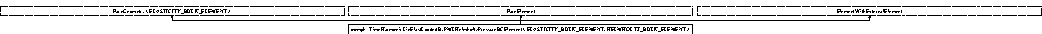
\includegraphics[height=0.454177cm]{classoomph_1_1TimeHarmonicLinElastLoadedByPMLHelmholtzPressureBCElement}
\end{center}
\end{figure}
\subsection*{Public Member Functions}
\begin{DoxyCompactItemize}
\item 
\hyperlink{classoomph_1_1TimeHarmonicLinElastLoadedByPMLHelmholtzPressureBCElement_aa22755297b70b0733797902787ffdcb1}{Time\+Harmonic\+Lin\+Elast\+Loaded\+By\+P\+M\+L\+Helmholtz\+Pressure\+B\+C\+Element} (Finite\+Element $\ast$const \&element\+\_\+pt, const int \&face\+\_\+index)
\begin{DoxyCompactList}\small\item\em Constructor, which takes a \char`\"{}bulk\char`\"{} element and the value of the index and its limit. \end{DoxyCompactList}\item 
void \hyperlink{classoomph_1_1TimeHarmonicLinElastLoadedByPMLHelmholtzPressureBCElement_a44261df2f1e5122ad707f17523a439c2}{fill\+\_\+in\+\_\+contribution\+\_\+to\+\_\+residuals} (Vector$<$ double $>$ \&residuals)
\begin{DoxyCompactList}\small\item\em Return the residuals. \end{DoxyCompactList}\item 
void \hyperlink{classoomph_1_1TimeHarmonicLinElastLoadedByPMLHelmholtzPressureBCElement_aec08514d7dbb65dc5c05af3131828daa}{fill\+\_\+in\+\_\+contribution\+\_\+to\+\_\+jacobian} (Vector$<$ double $>$ \&residuals, Dense\+Matrix$<$ double $>$ \&jacobian)
\begin{DoxyCompactList}\small\item\em Fill in contribution from Jacobian. \end{DoxyCompactList}\item 
const double \& \hyperlink{classoomph_1_1TimeHarmonicLinElastLoadedByPMLHelmholtzPressureBCElement_a9a010f4abd0ef1d311841b1a80b89495}{q} () const
\begin{DoxyCompactList}\small\item\em Return the ratio of the stress scales used to non-\/dimensionalise the fluid and elasticity equations. E.\+g. $ Q = (\omega a)^2 \rho/E $, i.\+e. the ratio between the inertial fluid stress and the solid\textquotesingle{}s elastic modulus E. \end{DoxyCompactList}\item 
double $\ast$\& \hyperlink{classoomph_1_1TimeHarmonicLinElastLoadedByPMLHelmholtzPressureBCElement_acec17c9c893e15d4d680d92f81a7f758}{q\+\_\+pt} ()
\begin{DoxyCompactList}\small\item\em Return a pointer the ratio of stress scales used to non-\/dimensionalise the fluid and solid equations. \end{DoxyCompactList}\item 
void \hyperlink{classoomph_1_1TimeHarmonicLinElastLoadedByPMLHelmholtzPressureBCElement_af349037cacaedb53f60de79415b83ac2}{output} (std\+::ostream \&outfile)
\begin{DoxyCompactList}\small\item\em Output function. \end{DoxyCompactList}\item 
void \hyperlink{classoomph_1_1TimeHarmonicLinElastLoadedByPMLHelmholtzPressureBCElement_a5b68e66db379729d4164df09dc00c681}{output} (std\+::ostream \&outfile, const unsigned \&n\+\_\+plot)
\begin{DoxyCompactList}\small\item\em Output function\+: Plot traction etc at Gauss points nplot is ignored. \end{DoxyCompactList}\item 
void \hyperlink{classoomph_1_1TimeHarmonicLinElastLoadedByPMLHelmholtzPressureBCElement_a1d9c27044ffbe07602f60ac7daef22af}{output} (F\+I\+LE $\ast$file\+\_\+pt)
\begin{DoxyCompactList}\small\item\em C\+\_\+style output function. \end{DoxyCompactList}\item 
void \hyperlink{classoomph_1_1TimeHarmonicLinElastLoadedByPMLHelmholtzPressureBCElement_a7e6d0ec6a0f9bec280fb4f520bf391f2}{output} (F\+I\+LE $\ast$file\+\_\+pt, const unsigned \&n\+\_\+plot)
\begin{DoxyCompactList}\small\item\em C-\/style output function. \end{DoxyCompactList}\item 
std\+::complex$<$ double $>$ \hyperlink{classoomph_1_1TimeHarmonicLinElastLoadedByPMLHelmholtzPressureBCElement_abd5ea8ff85472bc6c9d63d812142bd64}{global\+\_\+flux\+\_\+contribution\+\_\+from\+\_\+solid} ()
\begin{DoxyCompactList}\small\item\em Compute the global\+\_\+flux\+\_\+contribution through the template elasticity elements \+: we compute u.\+n. \end{DoxyCompactList}\item 
std\+::complex$<$ double $>$ \hyperlink{classoomph_1_1TimeHarmonicLinElastLoadedByPMLHelmholtzPressureBCElement_a75389b4a8d6180adf372bff670383e31}{global\+\_\+flux\+\_\+contribution\+\_\+from\+\_\+solid} (std\+::ofstream \&outfile)
\begin{DoxyCompactList}\small\item\em Compute the element\textquotesingle{}s contribution to the integral of the flux over the artificial boundary. Also output the flux in the specified output file if it\textquotesingle{}s open. \end{DoxyCompactList}\item 
std\+::complex$<$ double $>$ \hyperlink{classoomph_1_1TimeHarmonicLinElastLoadedByPMLHelmholtzPressureBCElement_a341e0b3eb0cc1d15d65bd95c8d3244a7}{global\+\_\+flux\+\_\+contribution\+\_\+from\+\_\+helmholtz} ()
\begin{DoxyCompactList}\small\item\em Compute the global\+\_\+flux\+\_\+contribution through the helmholtz elements \+: we compute dphidn.\+n. \end{DoxyCompactList}\item 
std\+::complex$<$ double $>$ \hyperlink{classoomph_1_1TimeHarmonicLinElastLoadedByPMLHelmholtzPressureBCElement_a9848b595cc22cd7fca0c862bdf59cc85}{global\+\_\+flux\+\_\+contribution\+\_\+from\+\_\+helmholtz} (std\+::ofstream \&outfile)
\begin{DoxyCompactList}\small\item\em Compute the element\textquotesingle{}s contribution to the integral of the flux over the artificial boundary. Also output the flux in the specified output file if it\textquotesingle{}s open. \end{DoxyCompactList}\end{DoxyCompactItemize}
\subsection*{Protected Member Functions}
\begin{DoxyCompactItemize}
\item 
void \hyperlink{classoomph_1_1TimeHarmonicLinElastLoadedByPMLHelmholtzPressureBCElement_a7012451bb562db8a3c8c07542699f6c8}{fill\+\_\+in\+\_\+contribution\+\_\+to\+\_\+residuals\+\_\+helmholtz\+\_\+traction} (Vector$<$ double $>$ \&residuals)
\begin{DoxyCompactList}\small\item\em Helper function that actually calculates the residuals. \end{DoxyCompactList}\end{DoxyCompactItemize}
\subsection*{Protected Attributes}
\begin{DoxyCompactItemize}
\item 
double $\ast$ \hyperlink{classoomph_1_1TimeHarmonicLinElastLoadedByPMLHelmholtzPressureBCElement_aa45224393afa639869972fdf77384e63}{Q\+\_\+pt}
\begin{DoxyCompactList}\small\item\em Pointer to the ratio, $ Q $ , of the stress used to non-\/dimensionalise the fluid stresses to the stress used to non-\/dimensionalise the solid stresses. \end{DoxyCompactList}\item 
Vector$<$ std\+::complex$<$ unsigned $>$ $>$ \hyperlink{classoomph_1_1TimeHarmonicLinElastLoadedByPMLHelmholtzPressureBCElement_a07cd6f158abf744ab24011d0d0a8a010}{U\+\_\+index\+\_\+time\+\_\+harmonic\+\_\+linear\+\_\+elasticity\+\_\+helmholtz\+\_\+traction}
\begin{DoxyCompactList}\small\item\em Index at which the i-\/th displacement component is stored. \end{DoxyCompactList}\end{DoxyCompactItemize}
\subsection*{Static Protected Attributes}
\begin{DoxyCompactItemize}
\item 
static double \hyperlink{classoomph_1_1TimeHarmonicLinElastLoadedByPMLHelmholtzPressureBCElement_a0f3bb2e8a6d9efe816f766b5e946f9c7}{Default\+\_\+\+Q\+\_\+\+Value} =1.\+0
\begin{DoxyCompactList}\small\item\em Static default value for the ratio of stress scales used in the fluid and solid equations (default is 1.\+0) \end{DoxyCompactList}\end{DoxyCompactItemize}


\subsection{Detailed Description}
\subsubsection*{template$<$class E\+L\+A\+S\+T\+I\+C\+I\+T\+Y\+\_\+\+B\+U\+L\+K\+\_\+\+E\+L\+E\+M\+E\+NT, class H\+E\+L\+M\+H\+O\+L\+T\+Z\+\_\+\+B\+U\+L\+K\+\_\+\+E\+L\+E\+M\+E\+NT$>$\newline
class oomph\+::\+Time\+Harmonic\+Lin\+Elast\+Loaded\+By\+P\+M\+L\+Helmholtz\+Pressure\+B\+C\+Element$<$ E\+L\+A\+S\+T\+I\+C\+I\+T\+Y\+\_\+\+B\+U\+L\+K\+\_\+\+E\+L\+E\+M\+E\+N\+T, H\+E\+L\+M\+H\+O\+L\+T\+Z\+\_\+\+B\+U\+L\+K\+\_\+\+E\+L\+E\+M\+E\+N\+T $>$}

A class for elements that allow the imposition of an applied traction in the equations of time-\/harmonic linear elasticity from a P\+M\+L\+Helmholtz potential (interpreted as a displacement potential for the fluid in a quasi-\/steady, linearised F\+SI problem.) The geometrical information can be read from the Face\+Geometry$<$\+E\+L\+E\+M\+E\+N\+T$>$ class and thus, we can be generic enough without the need to have a separate equations class. 

Definition at line 53 of file pml\+\_\+helmholtz\+\_\+time\+\_\+harmonic\+\_\+linear\+\_\+elasticity\+\_\+interaction.\+h.



\subsection{Constructor \& Destructor Documentation}
\mbox{\Hypertarget{classoomph_1_1TimeHarmonicLinElastLoadedByPMLHelmholtzPressureBCElement_aa22755297b70b0733797902787ffdcb1}\label{classoomph_1_1TimeHarmonicLinElastLoadedByPMLHelmholtzPressureBCElement_aa22755297b70b0733797902787ffdcb1}} 
\index{oomph\+::\+Time\+Harmonic\+Lin\+Elast\+Loaded\+By\+P\+M\+L\+Helmholtz\+Pressure\+B\+C\+Element@{oomph\+::\+Time\+Harmonic\+Lin\+Elast\+Loaded\+By\+P\+M\+L\+Helmholtz\+Pressure\+B\+C\+Element}!Time\+Harmonic\+Lin\+Elast\+Loaded\+By\+P\+M\+L\+Helmholtz\+Pressure\+B\+C\+Element@{Time\+Harmonic\+Lin\+Elast\+Loaded\+By\+P\+M\+L\+Helmholtz\+Pressure\+B\+C\+Element}}
\index{Time\+Harmonic\+Lin\+Elast\+Loaded\+By\+P\+M\+L\+Helmholtz\+Pressure\+B\+C\+Element@{Time\+Harmonic\+Lin\+Elast\+Loaded\+By\+P\+M\+L\+Helmholtz\+Pressure\+B\+C\+Element}!oomph\+::\+Time\+Harmonic\+Lin\+Elast\+Loaded\+By\+P\+M\+L\+Helmholtz\+Pressure\+B\+C\+Element@{oomph\+::\+Time\+Harmonic\+Lin\+Elast\+Loaded\+By\+P\+M\+L\+Helmholtz\+Pressure\+B\+C\+Element}}
\subsubsection{\texorpdfstring{Time\+Harmonic\+Lin\+Elast\+Loaded\+By\+P\+M\+L\+Helmholtz\+Pressure\+B\+C\+Element()}{TimeHarmonicLinElastLoadedByPMLHelmholtzPressureBCElement()}}
{\footnotesize\ttfamily template$<$class E\+L\+A\+S\+T\+I\+C\+I\+T\+Y\+\_\+\+B\+U\+L\+K\+\_\+\+E\+L\+E\+M\+E\+NT , class H\+E\+L\+M\+H\+O\+L\+T\+Z\+\_\+\+B\+U\+L\+K\+\_\+\+E\+L\+E\+M\+E\+NT $>$ \\
\hyperlink{classoomph_1_1TimeHarmonicLinElastLoadedByPMLHelmholtzPressureBCElement}{oomph\+::\+Time\+Harmonic\+Lin\+Elast\+Loaded\+By\+P\+M\+L\+Helmholtz\+Pressure\+B\+C\+Element}$<$ E\+L\+A\+S\+T\+I\+C\+I\+T\+Y\+\_\+\+B\+U\+L\+K\+\_\+\+E\+L\+E\+M\+E\+NT, H\+E\+L\+M\+H\+O\+L\+T\+Z\+\_\+\+B\+U\+L\+K\+\_\+\+E\+L\+E\+M\+E\+NT $>$\+::\hyperlink{classoomph_1_1TimeHarmonicLinElastLoadedByPMLHelmholtzPressureBCElement}{Time\+Harmonic\+Lin\+Elast\+Loaded\+By\+P\+M\+L\+Helmholtz\+Pressure\+B\+C\+Element} (\begin{DoxyParamCaption}\item[{Finite\+Element $\ast$const \&}]{element\+\_\+pt,  }\item[{const int \&}]{face\+\_\+index }\end{DoxyParamCaption})\hspace{0.3cm}{\ttfamily [inline]}}



Constructor, which takes a \char`\"{}bulk\char`\"{} element and the value of the index and its limit. 



Definition at line 85 of file pml\+\_\+helmholtz\+\_\+time\+\_\+harmonic\+\_\+linear\+\_\+elasticity\+\_\+interaction.\+h.



References oomph\+::\+Time\+Harmonic\+Lin\+Elast\+Loaded\+By\+P\+M\+L\+Helmholtz\+Pressure\+B\+C\+Element$<$ E\+L\+A\+S\+T\+I\+C\+I\+T\+Y\+\_\+\+B\+U\+L\+K\+\_\+\+E\+L\+E\+M\+E\+N\+T, H\+E\+L\+M\+H\+O\+L\+T\+Z\+\_\+\+B\+U\+L\+K\+\_\+\+E\+L\+E\+M\+E\+N\+T $>$\+::\+U\+\_\+index\+\_\+time\+\_\+harmonic\+\_\+linear\+\_\+elasticity\+\_\+helmholtz\+\_\+traction.



\subsection{Member Function Documentation}
\mbox{\Hypertarget{classoomph_1_1TimeHarmonicLinElastLoadedByPMLHelmholtzPressureBCElement_aec08514d7dbb65dc5c05af3131828daa}\label{classoomph_1_1TimeHarmonicLinElastLoadedByPMLHelmholtzPressureBCElement_aec08514d7dbb65dc5c05af3131828daa}} 
\index{oomph\+::\+Time\+Harmonic\+Lin\+Elast\+Loaded\+By\+P\+M\+L\+Helmholtz\+Pressure\+B\+C\+Element@{oomph\+::\+Time\+Harmonic\+Lin\+Elast\+Loaded\+By\+P\+M\+L\+Helmholtz\+Pressure\+B\+C\+Element}!fill\+\_\+in\+\_\+contribution\+\_\+to\+\_\+jacobian@{fill\+\_\+in\+\_\+contribution\+\_\+to\+\_\+jacobian}}
\index{fill\+\_\+in\+\_\+contribution\+\_\+to\+\_\+jacobian@{fill\+\_\+in\+\_\+contribution\+\_\+to\+\_\+jacobian}!oomph\+::\+Time\+Harmonic\+Lin\+Elast\+Loaded\+By\+P\+M\+L\+Helmholtz\+Pressure\+B\+C\+Element@{oomph\+::\+Time\+Harmonic\+Lin\+Elast\+Loaded\+By\+P\+M\+L\+Helmholtz\+Pressure\+B\+C\+Element}}
\subsubsection{\texorpdfstring{fill\+\_\+in\+\_\+contribution\+\_\+to\+\_\+jacobian()}{fill\_in\_contribution\_to\_jacobian()}}
{\footnotesize\ttfamily template$<$class E\+L\+A\+S\+T\+I\+C\+I\+T\+Y\+\_\+\+B\+U\+L\+K\+\_\+\+E\+L\+E\+M\+E\+NT , class H\+E\+L\+M\+H\+O\+L\+T\+Z\+\_\+\+B\+U\+L\+K\+\_\+\+E\+L\+E\+M\+E\+NT $>$ \\
void \hyperlink{classoomph_1_1TimeHarmonicLinElastLoadedByPMLHelmholtzPressureBCElement}{oomph\+::\+Time\+Harmonic\+Lin\+Elast\+Loaded\+By\+P\+M\+L\+Helmholtz\+Pressure\+B\+C\+Element}$<$ E\+L\+A\+S\+T\+I\+C\+I\+T\+Y\+\_\+\+B\+U\+L\+K\+\_\+\+E\+L\+E\+M\+E\+NT, H\+E\+L\+M\+H\+O\+L\+T\+Z\+\_\+\+B\+U\+L\+K\+\_\+\+E\+L\+E\+M\+E\+NT $>$\+::fill\+\_\+in\+\_\+contribution\+\_\+to\+\_\+jacobian (\begin{DoxyParamCaption}\item[{Vector$<$ double $>$ \&}]{residuals,  }\item[{Dense\+Matrix$<$ double $>$ \&}]{jacobian }\end{DoxyParamCaption})\hspace{0.3cm}{\ttfamily [inline]}}



Fill in contribution from Jacobian. 



Definition at line 150 of file pml\+\_\+helmholtz\+\_\+time\+\_\+harmonic\+\_\+linear\+\_\+elasticity\+\_\+interaction.\+h.



References oomph\+::\+Time\+Harmonic\+Lin\+Elast\+Loaded\+By\+P\+M\+L\+Helmholtz\+Pressure\+B\+C\+Element$<$ E\+L\+A\+S\+T\+I\+C\+I\+T\+Y\+\_\+\+B\+U\+L\+K\+\_\+\+E\+L\+E\+M\+E\+N\+T, H\+E\+L\+M\+H\+O\+L\+T\+Z\+\_\+\+B\+U\+L\+K\+\_\+\+E\+L\+E\+M\+E\+N\+T $>$\+::fill\+\_\+in\+\_\+contribution\+\_\+to\+\_\+residuals\+\_\+helmholtz\+\_\+traction().

\mbox{\Hypertarget{classoomph_1_1TimeHarmonicLinElastLoadedByPMLHelmholtzPressureBCElement_a44261df2f1e5122ad707f17523a439c2}\label{classoomph_1_1TimeHarmonicLinElastLoadedByPMLHelmholtzPressureBCElement_a44261df2f1e5122ad707f17523a439c2}} 
\index{oomph\+::\+Time\+Harmonic\+Lin\+Elast\+Loaded\+By\+P\+M\+L\+Helmholtz\+Pressure\+B\+C\+Element@{oomph\+::\+Time\+Harmonic\+Lin\+Elast\+Loaded\+By\+P\+M\+L\+Helmholtz\+Pressure\+B\+C\+Element}!fill\+\_\+in\+\_\+contribution\+\_\+to\+\_\+residuals@{fill\+\_\+in\+\_\+contribution\+\_\+to\+\_\+residuals}}
\index{fill\+\_\+in\+\_\+contribution\+\_\+to\+\_\+residuals@{fill\+\_\+in\+\_\+contribution\+\_\+to\+\_\+residuals}!oomph\+::\+Time\+Harmonic\+Lin\+Elast\+Loaded\+By\+P\+M\+L\+Helmholtz\+Pressure\+B\+C\+Element@{oomph\+::\+Time\+Harmonic\+Lin\+Elast\+Loaded\+By\+P\+M\+L\+Helmholtz\+Pressure\+B\+C\+Element}}
\subsubsection{\texorpdfstring{fill\+\_\+in\+\_\+contribution\+\_\+to\+\_\+residuals()}{fill\_in\_contribution\_to\_residuals()}}
{\footnotesize\ttfamily template$<$class E\+L\+A\+S\+T\+I\+C\+I\+T\+Y\+\_\+\+B\+U\+L\+K\+\_\+\+E\+L\+E\+M\+E\+NT , class H\+E\+L\+M\+H\+O\+L\+T\+Z\+\_\+\+B\+U\+L\+K\+\_\+\+E\+L\+E\+M\+E\+NT $>$ \\
void \hyperlink{classoomph_1_1TimeHarmonicLinElastLoadedByPMLHelmholtzPressureBCElement}{oomph\+::\+Time\+Harmonic\+Lin\+Elast\+Loaded\+By\+P\+M\+L\+Helmholtz\+Pressure\+B\+C\+Element}$<$ E\+L\+A\+S\+T\+I\+C\+I\+T\+Y\+\_\+\+B\+U\+L\+K\+\_\+\+E\+L\+E\+M\+E\+NT, H\+E\+L\+M\+H\+O\+L\+T\+Z\+\_\+\+B\+U\+L\+K\+\_\+\+E\+L\+E\+M\+E\+NT $>$\+::fill\+\_\+in\+\_\+contribution\+\_\+to\+\_\+residuals (\begin{DoxyParamCaption}\item[{Vector$<$ double $>$ \&}]{residuals }\end{DoxyParamCaption})\hspace{0.3cm}{\ttfamily [inline]}}



Return the residuals. 



Definition at line 142 of file pml\+\_\+helmholtz\+\_\+time\+\_\+harmonic\+\_\+linear\+\_\+elasticity\+\_\+interaction.\+h.



References oomph\+::\+Time\+Harmonic\+Lin\+Elast\+Loaded\+By\+P\+M\+L\+Helmholtz\+Pressure\+B\+C\+Element$<$ E\+L\+A\+S\+T\+I\+C\+I\+T\+Y\+\_\+\+B\+U\+L\+K\+\_\+\+E\+L\+E\+M\+E\+N\+T, H\+E\+L\+M\+H\+O\+L\+T\+Z\+\_\+\+B\+U\+L\+K\+\_\+\+E\+L\+E\+M\+E\+N\+T $>$\+::fill\+\_\+in\+\_\+contribution\+\_\+to\+\_\+residuals\+\_\+helmholtz\+\_\+traction().

\mbox{\Hypertarget{classoomph_1_1TimeHarmonicLinElastLoadedByPMLHelmholtzPressureBCElement_a7012451bb562db8a3c8c07542699f6c8}\label{classoomph_1_1TimeHarmonicLinElastLoadedByPMLHelmholtzPressureBCElement_a7012451bb562db8a3c8c07542699f6c8}} 
\index{oomph\+::\+Time\+Harmonic\+Lin\+Elast\+Loaded\+By\+P\+M\+L\+Helmholtz\+Pressure\+B\+C\+Element@{oomph\+::\+Time\+Harmonic\+Lin\+Elast\+Loaded\+By\+P\+M\+L\+Helmholtz\+Pressure\+B\+C\+Element}!fill\+\_\+in\+\_\+contribution\+\_\+to\+\_\+residuals\+\_\+helmholtz\+\_\+traction@{fill\+\_\+in\+\_\+contribution\+\_\+to\+\_\+residuals\+\_\+helmholtz\+\_\+traction}}
\index{fill\+\_\+in\+\_\+contribution\+\_\+to\+\_\+residuals\+\_\+helmholtz\+\_\+traction@{fill\+\_\+in\+\_\+contribution\+\_\+to\+\_\+residuals\+\_\+helmholtz\+\_\+traction}!oomph\+::\+Time\+Harmonic\+Lin\+Elast\+Loaded\+By\+P\+M\+L\+Helmholtz\+Pressure\+B\+C\+Element@{oomph\+::\+Time\+Harmonic\+Lin\+Elast\+Loaded\+By\+P\+M\+L\+Helmholtz\+Pressure\+B\+C\+Element}}
\subsubsection{\texorpdfstring{fill\+\_\+in\+\_\+contribution\+\_\+to\+\_\+residuals\+\_\+helmholtz\+\_\+traction()}{fill\_in\_contribution\_to\_residuals\_helmholtz\_traction()}}
{\footnotesize\ttfamily template$<$class E\+L\+A\+S\+T\+I\+C\+I\+T\+Y\+\_\+\+B\+U\+L\+K\+\_\+\+E\+L\+E\+M\+E\+NT , class H\+E\+L\+M\+H\+O\+L\+T\+Z\+\_\+\+B\+U\+L\+K\+\_\+\+E\+L\+E\+M\+E\+NT $>$ \\
void \hyperlink{classoomph_1_1TimeHarmonicLinElastLoadedByPMLHelmholtzPressureBCElement}{oomph\+::\+Time\+Harmonic\+Lin\+Elast\+Loaded\+By\+P\+M\+L\+Helmholtz\+Pressure\+B\+C\+Element}$<$ E\+L\+A\+S\+T\+I\+C\+I\+T\+Y\+\_\+\+B\+U\+L\+K\+\_\+\+E\+L\+E\+M\+E\+NT, H\+E\+L\+M\+H\+O\+L\+T\+Z\+\_\+\+B\+U\+L\+K\+\_\+\+E\+L\+E\+M\+E\+NT $>$\+::fill\+\_\+in\+\_\+contribution\+\_\+to\+\_\+residuals\+\_\+helmholtz\+\_\+traction (\begin{DoxyParamCaption}\item[{Vector$<$ double $>$ \&}]{residuals }\end{DoxyParamCaption})\hspace{0.3cm}{\ttfamily [protected]}}



Helper function that actually calculates the residuals. 

Return the residuals. 

Definition at line 517 of file pml\+\_\+helmholtz\+\_\+time\+\_\+harmonic\+\_\+linear\+\_\+elasticity\+\_\+interaction.\+h.



References oomph\+::\+Time\+Harmonic\+Lin\+Elast\+Loaded\+By\+P\+M\+L\+Helmholtz\+Pressure\+B\+C\+Element$<$ E\+L\+A\+S\+T\+I\+C\+I\+T\+Y\+\_\+\+B\+U\+L\+K\+\_\+\+E\+L\+E\+M\+E\+N\+T, H\+E\+L\+M\+H\+O\+L\+T\+Z\+\_\+\+B\+U\+L\+K\+\_\+\+E\+L\+E\+M\+E\+N\+T $>$\+::q(), and oomph\+::\+Time\+Harmonic\+Lin\+Elast\+Loaded\+By\+P\+M\+L\+Helmholtz\+Pressure\+B\+C\+Element$<$ E\+L\+A\+S\+T\+I\+C\+I\+T\+Y\+\_\+\+B\+U\+L\+K\+\_\+\+E\+L\+E\+M\+E\+N\+T, H\+E\+L\+M\+H\+O\+L\+T\+Z\+\_\+\+B\+U\+L\+K\+\_\+\+E\+L\+E\+M\+E\+N\+T $>$\+::\+U\+\_\+index\+\_\+time\+\_\+harmonic\+\_\+linear\+\_\+elasticity\+\_\+helmholtz\+\_\+traction.



Referenced by oomph\+::\+Time\+Harmonic\+Lin\+Elast\+Loaded\+By\+P\+M\+L\+Helmholtz\+Pressure\+B\+C\+Element$<$ E\+L\+A\+S\+T\+I\+C\+I\+T\+Y\+\_\+\+B\+U\+L\+K\+\_\+\+E\+L\+E\+M\+E\+N\+T, H\+E\+L\+M\+H\+O\+L\+T\+Z\+\_\+\+B\+U\+L\+K\+\_\+\+E\+L\+E\+M\+E\+N\+T $>$\+::fill\+\_\+in\+\_\+contribution\+\_\+to\+\_\+jacobian(), oomph\+::\+Time\+Harmonic\+Lin\+Elast\+Loaded\+By\+P\+M\+L\+Helmholtz\+Pressure\+B\+C\+Element$<$ E\+L\+A\+S\+T\+I\+C\+I\+T\+Y\+\_\+\+B\+U\+L\+K\+\_\+\+E\+L\+E\+M\+E\+N\+T, H\+E\+L\+M\+H\+O\+L\+T\+Z\+\_\+\+B\+U\+L\+K\+\_\+\+E\+L\+E\+M\+E\+N\+T $>$\+::fill\+\_\+in\+\_\+contribution\+\_\+to\+\_\+residuals(), and oomph\+::\+Time\+Harmonic\+Lin\+Elast\+Loaded\+By\+P\+M\+L\+Helmholtz\+Pressure\+B\+C\+Element$<$ E\+L\+A\+S\+T\+I\+C\+I\+T\+Y\+\_\+\+B\+U\+L\+K\+\_\+\+E\+L\+E\+M\+E\+N\+T, H\+E\+L\+M\+H\+O\+L\+T\+Z\+\_\+\+B\+U\+L\+K\+\_\+\+E\+L\+E\+M\+E\+N\+T $>$\+::global\+\_\+flux\+\_\+contribution\+\_\+from\+\_\+helmholtz().

\mbox{\Hypertarget{classoomph_1_1TimeHarmonicLinElastLoadedByPMLHelmholtzPressureBCElement_a341e0b3eb0cc1d15d65bd95c8d3244a7}\label{classoomph_1_1TimeHarmonicLinElastLoadedByPMLHelmholtzPressureBCElement_a341e0b3eb0cc1d15d65bd95c8d3244a7}} 
\index{oomph\+::\+Time\+Harmonic\+Lin\+Elast\+Loaded\+By\+P\+M\+L\+Helmholtz\+Pressure\+B\+C\+Element@{oomph\+::\+Time\+Harmonic\+Lin\+Elast\+Loaded\+By\+P\+M\+L\+Helmholtz\+Pressure\+B\+C\+Element}!global\+\_\+flux\+\_\+contribution\+\_\+from\+\_\+helmholtz@{global\+\_\+flux\+\_\+contribution\+\_\+from\+\_\+helmholtz}}
\index{global\+\_\+flux\+\_\+contribution\+\_\+from\+\_\+helmholtz@{global\+\_\+flux\+\_\+contribution\+\_\+from\+\_\+helmholtz}!oomph\+::\+Time\+Harmonic\+Lin\+Elast\+Loaded\+By\+P\+M\+L\+Helmholtz\+Pressure\+B\+C\+Element@{oomph\+::\+Time\+Harmonic\+Lin\+Elast\+Loaded\+By\+P\+M\+L\+Helmholtz\+Pressure\+B\+C\+Element}}
\subsubsection{\texorpdfstring{global\+\_\+flux\+\_\+contribution\+\_\+from\+\_\+helmholtz()}{global\_flux\_contribution\_from\_helmholtz()}\hspace{0.1cm}{\footnotesize\ttfamily [1/2]}}
{\footnotesize\ttfamily template$<$class E\+L\+A\+S\+T\+I\+C\+I\+T\+Y\+\_\+\+B\+U\+L\+K\+\_\+\+E\+L\+E\+M\+E\+NT , class H\+E\+L\+M\+H\+O\+L\+T\+Z\+\_\+\+B\+U\+L\+K\+\_\+\+E\+L\+E\+M\+E\+NT $>$ \\
std\+::complex$<$double$>$ \hyperlink{classoomph_1_1TimeHarmonicLinElastLoadedByPMLHelmholtzPressureBCElement}{oomph\+::\+Time\+Harmonic\+Lin\+Elast\+Loaded\+By\+P\+M\+L\+Helmholtz\+Pressure\+B\+C\+Element}$<$ E\+L\+A\+S\+T\+I\+C\+I\+T\+Y\+\_\+\+B\+U\+L\+K\+\_\+\+E\+L\+E\+M\+E\+NT, H\+E\+L\+M\+H\+O\+L\+T\+Z\+\_\+\+B\+U\+L\+K\+\_\+\+E\+L\+E\+M\+E\+NT $>$\+::global\+\_\+flux\+\_\+contribution\+\_\+from\+\_\+helmholtz (\begin{DoxyParamCaption}{ }\end{DoxyParamCaption})\hspace{0.3cm}{\ttfamily [inline]}}



Compute the global\+\_\+flux\+\_\+contribution through the helmholtz elements \+: we compute dphidn.\+n. 



Definition at line 351 of file pml\+\_\+helmholtz\+\_\+time\+\_\+harmonic\+\_\+linear\+\_\+elasticity\+\_\+interaction.\+h.

\mbox{\Hypertarget{classoomph_1_1TimeHarmonicLinElastLoadedByPMLHelmholtzPressureBCElement_a9848b595cc22cd7fca0c862bdf59cc85}\label{classoomph_1_1TimeHarmonicLinElastLoadedByPMLHelmholtzPressureBCElement_a9848b595cc22cd7fca0c862bdf59cc85}} 
\index{oomph\+::\+Time\+Harmonic\+Lin\+Elast\+Loaded\+By\+P\+M\+L\+Helmholtz\+Pressure\+B\+C\+Element@{oomph\+::\+Time\+Harmonic\+Lin\+Elast\+Loaded\+By\+P\+M\+L\+Helmholtz\+Pressure\+B\+C\+Element}!global\+\_\+flux\+\_\+contribution\+\_\+from\+\_\+helmholtz@{global\+\_\+flux\+\_\+contribution\+\_\+from\+\_\+helmholtz}}
\index{global\+\_\+flux\+\_\+contribution\+\_\+from\+\_\+helmholtz@{global\+\_\+flux\+\_\+contribution\+\_\+from\+\_\+helmholtz}!oomph\+::\+Time\+Harmonic\+Lin\+Elast\+Loaded\+By\+P\+M\+L\+Helmholtz\+Pressure\+B\+C\+Element@{oomph\+::\+Time\+Harmonic\+Lin\+Elast\+Loaded\+By\+P\+M\+L\+Helmholtz\+Pressure\+B\+C\+Element}}
\subsubsection{\texorpdfstring{global\+\_\+flux\+\_\+contribution\+\_\+from\+\_\+helmholtz()}{global\_flux\_contribution\_from\_helmholtz()}\hspace{0.1cm}{\footnotesize\ttfamily [2/2]}}
{\footnotesize\ttfamily template$<$class E\+L\+A\+S\+T\+I\+C\+I\+T\+Y\+\_\+\+B\+U\+L\+K\+\_\+\+E\+L\+E\+M\+E\+NT , class H\+E\+L\+M\+H\+O\+L\+T\+Z\+\_\+\+B\+U\+L\+K\+\_\+\+E\+L\+E\+M\+E\+NT $>$ \\
std\+::complex$<$double$>$ \hyperlink{classoomph_1_1TimeHarmonicLinElastLoadedByPMLHelmholtzPressureBCElement}{oomph\+::\+Time\+Harmonic\+Lin\+Elast\+Loaded\+By\+P\+M\+L\+Helmholtz\+Pressure\+B\+C\+Element}$<$ E\+L\+A\+S\+T\+I\+C\+I\+T\+Y\+\_\+\+B\+U\+L\+K\+\_\+\+E\+L\+E\+M\+E\+NT, H\+E\+L\+M\+H\+O\+L\+T\+Z\+\_\+\+B\+U\+L\+K\+\_\+\+E\+L\+E\+M\+E\+NT $>$\+::global\+\_\+flux\+\_\+contribution\+\_\+from\+\_\+helmholtz (\begin{DoxyParamCaption}\item[{std\+::ofstream \&}]{outfile }\end{DoxyParamCaption})\hspace{0.3cm}{\ttfamily [inline]}}



Compute the element\textquotesingle{}s contribution to the integral of the flux over the artificial boundary. Also output the flux in the specified output file if it\textquotesingle{}s open. 



Definition at line 362 of file pml\+\_\+helmholtz\+\_\+time\+\_\+harmonic\+\_\+linear\+\_\+elasticity\+\_\+interaction.\+h.



References oomph\+::\+Time\+Harmonic\+Lin\+Elast\+Loaded\+By\+P\+M\+L\+Helmholtz\+Pressure\+B\+C\+Element$<$ E\+L\+A\+S\+T\+I\+C\+I\+T\+Y\+\_\+\+B\+U\+L\+K\+\_\+\+E\+L\+E\+M\+E\+N\+T, H\+E\+L\+M\+H\+O\+L\+T\+Z\+\_\+\+B\+U\+L\+K\+\_\+\+E\+L\+E\+M\+E\+N\+T $>$\+::\+Default\+\_\+\+Q\+\_\+\+Value, and oomph\+::\+Time\+Harmonic\+Lin\+Elast\+Loaded\+By\+P\+M\+L\+Helmholtz\+Pressure\+B\+C\+Element$<$ E\+L\+A\+S\+T\+I\+C\+I\+T\+Y\+\_\+\+B\+U\+L\+K\+\_\+\+E\+L\+E\+M\+E\+N\+T, H\+E\+L\+M\+H\+O\+L\+T\+Z\+\_\+\+B\+U\+L\+K\+\_\+\+E\+L\+E\+M\+E\+N\+T $>$\+::fill\+\_\+in\+\_\+contribution\+\_\+to\+\_\+residuals\+\_\+helmholtz\+\_\+traction().

\mbox{\Hypertarget{classoomph_1_1TimeHarmonicLinElastLoadedByPMLHelmholtzPressureBCElement_abd5ea8ff85472bc6c9d63d812142bd64}\label{classoomph_1_1TimeHarmonicLinElastLoadedByPMLHelmholtzPressureBCElement_abd5ea8ff85472bc6c9d63d812142bd64}} 
\index{oomph\+::\+Time\+Harmonic\+Lin\+Elast\+Loaded\+By\+P\+M\+L\+Helmholtz\+Pressure\+B\+C\+Element@{oomph\+::\+Time\+Harmonic\+Lin\+Elast\+Loaded\+By\+P\+M\+L\+Helmholtz\+Pressure\+B\+C\+Element}!global\+\_\+flux\+\_\+contribution\+\_\+from\+\_\+solid@{global\+\_\+flux\+\_\+contribution\+\_\+from\+\_\+solid}}
\index{global\+\_\+flux\+\_\+contribution\+\_\+from\+\_\+solid@{global\+\_\+flux\+\_\+contribution\+\_\+from\+\_\+solid}!oomph\+::\+Time\+Harmonic\+Lin\+Elast\+Loaded\+By\+P\+M\+L\+Helmholtz\+Pressure\+B\+C\+Element@{oomph\+::\+Time\+Harmonic\+Lin\+Elast\+Loaded\+By\+P\+M\+L\+Helmholtz\+Pressure\+B\+C\+Element}}
\subsubsection{\texorpdfstring{global\+\_\+flux\+\_\+contribution\+\_\+from\+\_\+solid()}{global\_flux\_contribution\_from\_solid()}\hspace{0.1cm}{\footnotesize\ttfamily [1/2]}}
{\footnotesize\ttfamily template$<$class E\+L\+A\+S\+T\+I\+C\+I\+T\+Y\+\_\+\+B\+U\+L\+K\+\_\+\+E\+L\+E\+M\+E\+NT , class H\+E\+L\+M\+H\+O\+L\+T\+Z\+\_\+\+B\+U\+L\+K\+\_\+\+E\+L\+E\+M\+E\+NT $>$ \\
std\+::complex$<$double$>$ \hyperlink{classoomph_1_1TimeHarmonicLinElastLoadedByPMLHelmholtzPressureBCElement}{oomph\+::\+Time\+Harmonic\+Lin\+Elast\+Loaded\+By\+P\+M\+L\+Helmholtz\+Pressure\+B\+C\+Element}$<$ E\+L\+A\+S\+T\+I\+C\+I\+T\+Y\+\_\+\+B\+U\+L\+K\+\_\+\+E\+L\+E\+M\+E\+NT, H\+E\+L\+M\+H\+O\+L\+T\+Z\+\_\+\+B\+U\+L\+K\+\_\+\+E\+L\+E\+M\+E\+NT $>$\+::global\+\_\+flux\+\_\+contribution\+\_\+from\+\_\+solid (\begin{DoxyParamCaption}{ }\end{DoxyParamCaption})\hspace{0.3cm}{\ttfamily [inline]}}



Compute the global\+\_\+flux\+\_\+contribution through the template elasticity elements \+: we compute u.\+n. 



Definition at line 258 of file pml\+\_\+helmholtz\+\_\+time\+\_\+harmonic\+\_\+linear\+\_\+elasticity\+\_\+interaction.\+h.

\mbox{\Hypertarget{classoomph_1_1TimeHarmonicLinElastLoadedByPMLHelmholtzPressureBCElement_a75389b4a8d6180adf372bff670383e31}\label{classoomph_1_1TimeHarmonicLinElastLoadedByPMLHelmholtzPressureBCElement_a75389b4a8d6180adf372bff670383e31}} 
\index{oomph\+::\+Time\+Harmonic\+Lin\+Elast\+Loaded\+By\+P\+M\+L\+Helmholtz\+Pressure\+B\+C\+Element@{oomph\+::\+Time\+Harmonic\+Lin\+Elast\+Loaded\+By\+P\+M\+L\+Helmholtz\+Pressure\+B\+C\+Element}!global\+\_\+flux\+\_\+contribution\+\_\+from\+\_\+solid@{global\+\_\+flux\+\_\+contribution\+\_\+from\+\_\+solid}}
\index{global\+\_\+flux\+\_\+contribution\+\_\+from\+\_\+solid@{global\+\_\+flux\+\_\+contribution\+\_\+from\+\_\+solid}!oomph\+::\+Time\+Harmonic\+Lin\+Elast\+Loaded\+By\+P\+M\+L\+Helmholtz\+Pressure\+B\+C\+Element@{oomph\+::\+Time\+Harmonic\+Lin\+Elast\+Loaded\+By\+P\+M\+L\+Helmholtz\+Pressure\+B\+C\+Element}}
\subsubsection{\texorpdfstring{global\+\_\+flux\+\_\+contribution\+\_\+from\+\_\+solid()}{global\_flux\_contribution\_from\_solid()}\hspace{0.1cm}{\footnotesize\ttfamily [2/2]}}
{\footnotesize\ttfamily template$<$class E\+L\+A\+S\+T\+I\+C\+I\+T\+Y\+\_\+\+B\+U\+L\+K\+\_\+\+E\+L\+E\+M\+E\+NT , class H\+E\+L\+M\+H\+O\+L\+T\+Z\+\_\+\+B\+U\+L\+K\+\_\+\+E\+L\+E\+M\+E\+NT $>$ \\
std\+::complex$<$double$>$ \hyperlink{classoomph_1_1TimeHarmonicLinElastLoadedByPMLHelmholtzPressureBCElement}{oomph\+::\+Time\+Harmonic\+Lin\+Elast\+Loaded\+By\+P\+M\+L\+Helmholtz\+Pressure\+B\+C\+Element}$<$ E\+L\+A\+S\+T\+I\+C\+I\+T\+Y\+\_\+\+B\+U\+L\+K\+\_\+\+E\+L\+E\+M\+E\+NT, H\+E\+L\+M\+H\+O\+L\+T\+Z\+\_\+\+B\+U\+L\+K\+\_\+\+E\+L\+E\+M\+E\+NT $>$\+::global\+\_\+flux\+\_\+contribution\+\_\+from\+\_\+solid (\begin{DoxyParamCaption}\item[{std\+::ofstream \&}]{outfile }\end{DoxyParamCaption})\hspace{0.3cm}{\ttfamily [inline]}}



Compute the element\textquotesingle{}s contribution to the integral of the flux over the artificial boundary. Also output the flux in the specified output file if it\textquotesingle{}s open. 



Definition at line 269 of file pml\+\_\+helmholtz\+\_\+time\+\_\+harmonic\+\_\+linear\+\_\+elasticity\+\_\+interaction.\+h.

\mbox{\Hypertarget{classoomph_1_1TimeHarmonicLinElastLoadedByPMLHelmholtzPressureBCElement_af349037cacaedb53f60de79415b83ac2}\label{classoomph_1_1TimeHarmonicLinElastLoadedByPMLHelmholtzPressureBCElement_af349037cacaedb53f60de79415b83ac2}} 
\index{oomph\+::\+Time\+Harmonic\+Lin\+Elast\+Loaded\+By\+P\+M\+L\+Helmholtz\+Pressure\+B\+C\+Element@{oomph\+::\+Time\+Harmonic\+Lin\+Elast\+Loaded\+By\+P\+M\+L\+Helmholtz\+Pressure\+B\+C\+Element}!output@{output}}
\index{output@{output}!oomph\+::\+Time\+Harmonic\+Lin\+Elast\+Loaded\+By\+P\+M\+L\+Helmholtz\+Pressure\+B\+C\+Element@{oomph\+::\+Time\+Harmonic\+Lin\+Elast\+Loaded\+By\+P\+M\+L\+Helmholtz\+Pressure\+B\+C\+Element}}
\subsubsection{\texorpdfstring{output()}{output()}\hspace{0.1cm}{\footnotesize\ttfamily [1/4]}}
{\footnotesize\ttfamily template$<$class E\+L\+A\+S\+T\+I\+C\+I\+T\+Y\+\_\+\+B\+U\+L\+K\+\_\+\+E\+L\+E\+M\+E\+NT , class H\+E\+L\+M\+H\+O\+L\+T\+Z\+\_\+\+B\+U\+L\+K\+\_\+\+E\+L\+E\+M\+E\+NT $>$ \\
void \hyperlink{classoomph_1_1TimeHarmonicLinElastLoadedByPMLHelmholtzPressureBCElement}{oomph\+::\+Time\+Harmonic\+Lin\+Elast\+Loaded\+By\+P\+M\+L\+Helmholtz\+Pressure\+B\+C\+Element}$<$ E\+L\+A\+S\+T\+I\+C\+I\+T\+Y\+\_\+\+B\+U\+L\+K\+\_\+\+E\+L\+E\+M\+E\+NT, H\+E\+L\+M\+H\+O\+L\+T\+Z\+\_\+\+B\+U\+L\+K\+\_\+\+E\+L\+E\+M\+E\+NT $>$\+::output (\begin{DoxyParamCaption}\item[{std\+::ostream \&}]{outfile }\end{DoxyParamCaption})\hspace{0.3cm}{\ttfamily [inline]}}



Output function. 

Dummy 

Definition at line 173 of file pml\+\_\+helmholtz\+\_\+time\+\_\+harmonic\+\_\+linear\+\_\+elasticity\+\_\+interaction.\+h.



Referenced by oomph\+::\+P\+M\+L\+Helmholtz\+Flux\+From\+Normal\+Displacement\+B\+C\+Element$<$ H\+E\+L\+M\+H\+O\+L\+T\+Z\+\_\+\+B\+U\+L\+K\+\_\+\+E\+L\+E\+M\+E\+N\+T, E\+L\+A\+S\+T\+I\+C\+I\+T\+Y\+\_\+\+B\+U\+L\+K\+\_\+\+E\+L\+E\+M\+E\+N\+T $>$\+::output().

\mbox{\Hypertarget{classoomph_1_1TimeHarmonicLinElastLoadedByPMLHelmholtzPressureBCElement_a5b68e66db379729d4164df09dc00c681}\label{classoomph_1_1TimeHarmonicLinElastLoadedByPMLHelmholtzPressureBCElement_a5b68e66db379729d4164df09dc00c681}} 
\index{oomph\+::\+Time\+Harmonic\+Lin\+Elast\+Loaded\+By\+P\+M\+L\+Helmholtz\+Pressure\+B\+C\+Element@{oomph\+::\+Time\+Harmonic\+Lin\+Elast\+Loaded\+By\+P\+M\+L\+Helmholtz\+Pressure\+B\+C\+Element}!output@{output}}
\index{output@{output}!oomph\+::\+Time\+Harmonic\+Lin\+Elast\+Loaded\+By\+P\+M\+L\+Helmholtz\+Pressure\+B\+C\+Element@{oomph\+::\+Time\+Harmonic\+Lin\+Elast\+Loaded\+By\+P\+M\+L\+Helmholtz\+Pressure\+B\+C\+Element}}
\subsubsection{\texorpdfstring{output()}{output()}\hspace{0.1cm}{\footnotesize\ttfamily [2/4]}}
{\footnotesize\ttfamily template$<$class E\+L\+A\+S\+T\+I\+C\+I\+T\+Y\+\_\+\+B\+U\+L\+K\+\_\+\+E\+L\+E\+M\+E\+NT , class H\+E\+L\+M\+H\+O\+L\+T\+Z\+\_\+\+B\+U\+L\+K\+\_\+\+E\+L\+E\+M\+E\+NT $>$ \\
void \hyperlink{classoomph_1_1TimeHarmonicLinElastLoadedByPMLHelmholtzPressureBCElement}{oomph\+::\+Time\+Harmonic\+Lin\+Elast\+Loaded\+By\+P\+M\+L\+Helmholtz\+Pressure\+B\+C\+Element}$<$ E\+L\+A\+S\+T\+I\+C\+I\+T\+Y\+\_\+\+B\+U\+L\+K\+\_\+\+E\+L\+E\+M\+E\+NT, H\+E\+L\+M\+H\+O\+L\+T\+Z\+\_\+\+B\+U\+L\+K\+\_\+\+E\+L\+E\+M\+E\+NT $>$\+::output (\begin{DoxyParamCaption}\item[{std\+::ostream \&}]{outfile,  }\item[{const unsigned \&}]{n\+\_\+plot }\end{DoxyParamCaption})\hspace{0.3cm}{\ttfamily [inline]}}



Output function\+: Plot traction etc at Gauss points nplot is ignored. 



Definition at line 182 of file pml\+\_\+helmholtz\+\_\+time\+\_\+harmonic\+\_\+linear\+\_\+elasticity\+\_\+interaction.\+h.



References oomph\+::\+Time\+Harmonic\+Lin\+Elast\+Loaded\+By\+P\+M\+L\+Helmholtz\+Pressure\+B\+C\+Element$<$ E\+L\+A\+S\+T\+I\+C\+I\+T\+Y\+\_\+\+B\+U\+L\+K\+\_\+\+E\+L\+E\+M\+E\+N\+T, H\+E\+L\+M\+H\+O\+L\+T\+Z\+\_\+\+B\+U\+L\+K\+\_\+\+E\+L\+E\+M\+E\+N\+T $>$\+::q().

\mbox{\Hypertarget{classoomph_1_1TimeHarmonicLinElastLoadedByPMLHelmholtzPressureBCElement_a1d9c27044ffbe07602f60ac7daef22af}\label{classoomph_1_1TimeHarmonicLinElastLoadedByPMLHelmholtzPressureBCElement_a1d9c27044ffbe07602f60ac7daef22af}} 
\index{oomph\+::\+Time\+Harmonic\+Lin\+Elast\+Loaded\+By\+P\+M\+L\+Helmholtz\+Pressure\+B\+C\+Element@{oomph\+::\+Time\+Harmonic\+Lin\+Elast\+Loaded\+By\+P\+M\+L\+Helmholtz\+Pressure\+B\+C\+Element}!output@{output}}
\index{output@{output}!oomph\+::\+Time\+Harmonic\+Lin\+Elast\+Loaded\+By\+P\+M\+L\+Helmholtz\+Pressure\+B\+C\+Element@{oomph\+::\+Time\+Harmonic\+Lin\+Elast\+Loaded\+By\+P\+M\+L\+Helmholtz\+Pressure\+B\+C\+Element}}
\subsubsection{\texorpdfstring{output()}{output()}\hspace{0.1cm}{\footnotesize\ttfamily [3/4]}}
{\footnotesize\ttfamily template$<$class E\+L\+A\+S\+T\+I\+C\+I\+T\+Y\+\_\+\+B\+U\+L\+K\+\_\+\+E\+L\+E\+M\+E\+NT , class H\+E\+L\+M\+H\+O\+L\+T\+Z\+\_\+\+B\+U\+L\+K\+\_\+\+E\+L\+E\+M\+E\+NT $>$ \\
void \hyperlink{classoomph_1_1TimeHarmonicLinElastLoadedByPMLHelmholtzPressureBCElement}{oomph\+::\+Time\+Harmonic\+Lin\+Elast\+Loaded\+By\+P\+M\+L\+Helmholtz\+Pressure\+B\+C\+Element}$<$ E\+L\+A\+S\+T\+I\+C\+I\+T\+Y\+\_\+\+B\+U\+L\+K\+\_\+\+E\+L\+E\+M\+E\+NT, H\+E\+L\+M\+H\+O\+L\+T\+Z\+\_\+\+B\+U\+L\+K\+\_\+\+E\+L\+E\+M\+E\+NT $>$\+::output (\begin{DoxyParamCaption}\item[{F\+I\+LE $\ast$}]{file\+\_\+pt }\end{DoxyParamCaption})\hspace{0.3cm}{\ttfamily [inline]}}



C\+\_\+style output function. 



Definition at line 249 of file pml\+\_\+helmholtz\+\_\+time\+\_\+harmonic\+\_\+linear\+\_\+elasticity\+\_\+interaction.\+h.

\mbox{\Hypertarget{classoomph_1_1TimeHarmonicLinElastLoadedByPMLHelmholtzPressureBCElement_a7e6d0ec6a0f9bec280fb4f520bf391f2}\label{classoomph_1_1TimeHarmonicLinElastLoadedByPMLHelmholtzPressureBCElement_a7e6d0ec6a0f9bec280fb4f520bf391f2}} 
\index{oomph\+::\+Time\+Harmonic\+Lin\+Elast\+Loaded\+By\+P\+M\+L\+Helmholtz\+Pressure\+B\+C\+Element@{oomph\+::\+Time\+Harmonic\+Lin\+Elast\+Loaded\+By\+P\+M\+L\+Helmholtz\+Pressure\+B\+C\+Element}!output@{output}}
\index{output@{output}!oomph\+::\+Time\+Harmonic\+Lin\+Elast\+Loaded\+By\+P\+M\+L\+Helmholtz\+Pressure\+B\+C\+Element@{oomph\+::\+Time\+Harmonic\+Lin\+Elast\+Loaded\+By\+P\+M\+L\+Helmholtz\+Pressure\+B\+C\+Element}}
\subsubsection{\texorpdfstring{output()}{output()}\hspace{0.1cm}{\footnotesize\ttfamily [4/4]}}
{\footnotesize\ttfamily template$<$class E\+L\+A\+S\+T\+I\+C\+I\+T\+Y\+\_\+\+B\+U\+L\+K\+\_\+\+E\+L\+E\+M\+E\+NT , class H\+E\+L\+M\+H\+O\+L\+T\+Z\+\_\+\+B\+U\+L\+K\+\_\+\+E\+L\+E\+M\+E\+NT $>$ \\
void \hyperlink{classoomph_1_1TimeHarmonicLinElastLoadedByPMLHelmholtzPressureBCElement}{oomph\+::\+Time\+Harmonic\+Lin\+Elast\+Loaded\+By\+P\+M\+L\+Helmholtz\+Pressure\+B\+C\+Element}$<$ E\+L\+A\+S\+T\+I\+C\+I\+T\+Y\+\_\+\+B\+U\+L\+K\+\_\+\+E\+L\+E\+M\+E\+NT, H\+E\+L\+M\+H\+O\+L\+T\+Z\+\_\+\+B\+U\+L\+K\+\_\+\+E\+L\+E\+M\+E\+NT $>$\+::output (\begin{DoxyParamCaption}\item[{F\+I\+LE $\ast$}]{file\+\_\+pt,  }\item[{const unsigned \&}]{n\+\_\+plot }\end{DoxyParamCaption})\hspace{0.3cm}{\ttfamily [inline]}}



C-\/style output function. 



Definition at line 253 of file pml\+\_\+helmholtz\+\_\+time\+\_\+harmonic\+\_\+linear\+\_\+elasticity\+\_\+interaction.\+h.

\mbox{\Hypertarget{classoomph_1_1TimeHarmonicLinElastLoadedByPMLHelmholtzPressureBCElement_a9a010f4abd0ef1d311841b1a80b89495}\label{classoomph_1_1TimeHarmonicLinElastLoadedByPMLHelmholtzPressureBCElement_a9a010f4abd0ef1d311841b1a80b89495}} 
\index{oomph\+::\+Time\+Harmonic\+Lin\+Elast\+Loaded\+By\+P\+M\+L\+Helmholtz\+Pressure\+B\+C\+Element@{oomph\+::\+Time\+Harmonic\+Lin\+Elast\+Loaded\+By\+P\+M\+L\+Helmholtz\+Pressure\+B\+C\+Element}!q@{q}}
\index{q@{q}!oomph\+::\+Time\+Harmonic\+Lin\+Elast\+Loaded\+By\+P\+M\+L\+Helmholtz\+Pressure\+B\+C\+Element@{oomph\+::\+Time\+Harmonic\+Lin\+Elast\+Loaded\+By\+P\+M\+L\+Helmholtz\+Pressure\+B\+C\+Element}}
\subsubsection{\texorpdfstring{q()}{q()}}
{\footnotesize\ttfamily template$<$class E\+L\+A\+S\+T\+I\+C\+I\+T\+Y\+\_\+\+B\+U\+L\+K\+\_\+\+E\+L\+E\+M\+E\+NT , class H\+E\+L\+M\+H\+O\+L\+T\+Z\+\_\+\+B\+U\+L\+K\+\_\+\+E\+L\+E\+M\+E\+NT $>$ \\
const double\& \hyperlink{classoomph_1_1TimeHarmonicLinElastLoadedByPMLHelmholtzPressureBCElement}{oomph\+::\+Time\+Harmonic\+Lin\+Elast\+Loaded\+By\+P\+M\+L\+Helmholtz\+Pressure\+B\+C\+Element}$<$ E\+L\+A\+S\+T\+I\+C\+I\+T\+Y\+\_\+\+B\+U\+L\+K\+\_\+\+E\+L\+E\+M\+E\+NT, H\+E\+L\+M\+H\+O\+L\+T\+Z\+\_\+\+B\+U\+L\+K\+\_\+\+E\+L\+E\+M\+E\+NT $>$\+::q (\begin{DoxyParamCaption}{ }\end{DoxyParamCaption}) const\hspace{0.3cm}{\ttfamily [inline]}}



Return the ratio of the stress scales used to non-\/dimensionalise the fluid and elasticity equations. E.\+g. $ Q = (\omega a)^2 \rho/E $, i.\+e. the ratio between the inertial fluid stress and the solid\textquotesingle{}s elastic modulus E. 



Definition at line 165 of file pml\+\_\+helmholtz\+\_\+time\+\_\+harmonic\+\_\+linear\+\_\+elasticity\+\_\+interaction.\+h.



References oomph\+::\+Time\+Harmonic\+Lin\+Elast\+Loaded\+By\+P\+M\+L\+Helmholtz\+Pressure\+B\+C\+Element$<$ E\+L\+A\+S\+T\+I\+C\+I\+T\+Y\+\_\+\+B\+U\+L\+K\+\_\+\+E\+L\+E\+M\+E\+N\+T, H\+E\+L\+M\+H\+O\+L\+T\+Z\+\_\+\+B\+U\+L\+K\+\_\+\+E\+L\+E\+M\+E\+N\+T $>$\+::\+Q\+\_\+pt.



Referenced by oomph\+::\+Time\+Harmonic\+Lin\+Elast\+Loaded\+By\+P\+M\+L\+Helmholtz\+Pressure\+B\+C\+Element$<$ E\+L\+A\+S\+T\+I\+C\+I\+T\+Y\+\_\+\+B\+U\+L\+K\+\_\+\+E\+L\+E\+M\+E\+N\+T, H\+E\+L\+M\+H\+O\+L\+T\+Z\+\_\+\+B\+U\+L\+K\+\_\+\+E\+L\+E\+M\+E\+N\+T $>$\+::fill\+\_\+in\+\_\+contribution\+\_\+to\+\_\+residuals\+\_\+helmholtz\+\_\+traction(), and oomph\+::\+Time\+Harmonic\+Lin\+Elast\+Loaded\+By\+P\+M\+L\+Helmholtz\+Pressure\+B\+C\+Element$<$ E\+L\+A\+S\+T\+I\+C\+I\+T\+Y\+\_\+\+B\+U\+L\+K\+\_\+\+E\+L\+E\+M\+E\+N\+T, H\+E\+L\+M\+H\+O\+L\+T\+Z\+\_\+\+B\+U\+L\+K\+\_\+\+E\+L\+E\+M\+E\+N\+T $>$\+::output().

\mbox{\Hypertarget{classoomph_1_1TimeHarmonicLinElastLoadedByPMLHelmholtzPressureBCElement_acec17c9c893e15d4d680d92f81a7f758}\label{classoomph_1_1TimeHarmonicLinElastLoadedByPMLHelmholtzPressureBCElement_acec17c9c893e15d4d680d92f81a7f758}} 
\index{oomph\+::\+Time\+Harmonic\+Lin\+Elast\+Loaded\+By\+P\+M\+L\+Helmholtz\+Pressure\+B\+C\+Element@{oomph\+::\+Time\+Harmonic\+Lin\+Elast\+Loaded\+By\+P\+M\+L\+Helmholtz\+Pressure\+B\+C\+Element}!q\+\_\+pt@{q\+\_\+pt}}
\index{q\+\_\+pt@{q\+\_\+pt}!oomph\+::\+Time\+Harmonic\+Lin\+Elast\+Loaded\+By\+P\+M\+L\+Helmholtz\+Pressure\+B\+C\+Element@{oomph\+::\+Time\+Harmonic\+Lin\+Elast\+Loaded\+By\+P\+M\+L\+Helmholtz\+Pressure\+B\+C\+Element}}
\subsubsection{\texorpdfstring{q\+\_\+pt()}{q\_pt()}}
{\footnotesize\ttfamily template$<$class E\+L\+A\+S\+T\+I\+C\+I\+T\+Y\+\_\+\+B\+U\+L\+K\+\_\+\+E\+L\+E\+M\+E\+NT , class H\+E\+L\+M\+H\+O\+L\+T\+Z\+\_\+\+B\+U\+L\+K\+\_\+\+E\+L\+E\+M\+E\+NT $>$ \\
double$\ast$ \& \hyperlink{classoomph_1_1TimeHarmonicLinElastLoadedByPMLHelmholtzPressureBCElement}{oomph\+::\+Time\+Harmonic\+Lin\+Elast\+Loaded\+By\+P\+M\+L\+Helmholtz\+Pressure\+B\+C\+Element}$<$ E\+L\+A\+S\+T\+I\+C\+I\+T\+Y\+\_\+\+B\+U\+L\+K\+\_\+\+E\+L\+E\+M\+E\+NT, H\+E\+L\+M\+H\+O\+L\+T\+Z\+\_\+\+B\+U\+L\+K\+\_\+\+E\+L\+E\+M\+E\+NT $>$\+::q\+\_\+pt (\begin{DoxyParamCaption}{ }\end{DoxyParamCaption})\hspace{0.3cm}{\ttfamily [inline]}}



Return a pointer the ratio of stress scales used to non-\/dimensionalise the fluid and solid equations. 



Definition at line 169 of file pml\+\_\+helmholtz\+\_\+time\+\_\+harmonic\+\_\+linear\+\_\+elasticity\+\_\+interaction.\+h.



References oomph\+::\+Time\+Harmonic\+Lin\+Elast\+Loaded\+By\+P\+M\+L\+Helmholtz\+Pressure\+B\+C\+Element$<$ E\+L\+A\+S\+T\+I\+C\+I\+T\+Y\+\_\+\+B\+U\+L\+K\+\_\+\+E\+L\+E\+M\+E\+N\+T, H\+E\+L\+M\+H\+O\+L\+T\+Z\+\_\+\+B\+U\+L\+K\+\_\+\+E\+L\+E\+M\+E\+N\+T $>$\+::\+Q\+\_\+pt.



\subsection{Member Data Documentation}
\mbox{\Hypertarget{classoomph_1_1TimeHarmonicLinElastLoadedByPMLHelmholtzPressureBCElement_a0f3bb2e8a6d9efe816f766b5e946f9c7}\label{classoomph_1_1TimeHarmonicLinElastLoadedByPMLHelmholtzPressureBCElement_a0f3bb2e8a6d9efe816f766b5e946f9c7}} 
\index{oomph\+::\+Time\+Harmonic\+Lin\+Elast\+Loaded\+By\+P\+M\+L\+Helmholtz\+Pressure\+B\+C\+Element@{oomph\+::\+Time\+Harmonic\+Lin\+Elast\+Loaded\+By\+P\+M\+L\+Helmholtz\+Pressure\+B\+C\+Element}!Default\+\_\+\+Q\+\_\+\+Value@{Default\+\_\+\+Q\+\_\+\+Value}}
\index{Default\+\_\+\+Q\+\_\+\+Value@{Default\+\_\+\+Q\+\_\+\+Value}!oomph\+::\+Time\+Harmonic\+Lin\+Elast\+Loaded\+By\+P\+M\+L\+Helmholtz\+Pressure\+B\+C\+Element@{oomph\+::\+Time\+Harmonic\+Lin\+Elast\+Loaded\+By\+P\+M\+L\+Helmholtz\+Pressure\+B\+C\+Element}}
\subsubsection{\texorpdfstring{Default\+\_\+\+Q\+\_\+\+Value}{Default\_Q\_Value}}
{\footnotesize\ttfamily template$<$class E\+L\+A\+S\+T\+I\+C\+I\+T\+Y\+\_\+\+B\+U\+L\+K\+\_\+\+E\+L\+E\+M\+E\+NT , class H\+E\+L\+M\+H\+O\+L\+T\+Z\+\_\+\+B\+U\+L\+K\+\_\+\+E\+L\+E\+M\+E\+NT $>$ \\
double \hyperlink{classoomph_1_1TimeHarmonicLinElastLoadedByPMLHelmholtzPressureBCElement}{oomph\+::\+Time\+Harmonic\+Lin\+Elast\+Loaded\+By\+P\+M\+L\+Helmholtz\+Pressure\+B\+C\+Element}$<$ E\+L\+A\+S\+T\+I\+C\+I\+T\+Y\+\_\+\+B\+U\+L\+K\+\_\+\+E\+L\+E\+M\+E\+NT, H\+E\+L\+M\+H\+O\+L\+T\+Z\+\_\+\+B\+U\+L\+K\+\_\+\+E\+L\+E\+M\+E\+NT $>$\+::Default\+\_\+\+Q\+\_\+\+Value =1.\+0\hspace{0.3cm}{\ttfamily [static]}, {\ttfamily [protected]}}



Static default value for the ratio of stress scales used in the fluid and solid equations (default is 1.\+0) 

Static default value for the ragoogletio of stress scales used in the fluid and solid equations (default is 1.\+0) 

Definition at line 68 of file pml\+\_\+helmholtz\+\_\+time\+\_\+harmonic\+\_\+linear\+\_\+elasticity\+\_\+interaction.\+h.



Referenced by oomph\+::\+Time\+Harmonic\+Lin\+Elast\+Loaded\+By\+P\+M\+L\+Helmholtz\+Pressure\+B\+C\+Element$<$ E\+L\+A\+S\+T\+I\+C\+I\+T\+Y\+\_\+\+B\+U\+L\+K\+\_\+\+E\+L\+E\+M\+E\+N\+T, H\+E\+L\+M\+H\+O\+L\+T\+Z\+\_\+\+B\+U\+L\+K\+\_\+\+E\+L\+E\+M\+E\+N\+T $>$\+::global\+\_\+flux\+\_\+contribution\+\_\+from\+\_\+helmholtz().

\mbox{\Hypertarget{classoomph_1_1TimeHarmonicLinElastLoadedByPMLHelmholtzPressureBCElement_aa45224393afa639869972fdf77384e63}\label{classoomph_1_1TimeHarmonicLinElastLoadedByPMLHelmholtzPressureBCElement_aa45224393afa639869972fdf77384e63}} 
\index{oomph\+::\+Time\+Harmonic\+Lin\+Elast\+Loaded\+By\+P\+M\+L\+Helmholtz\+Pressure\+B\+C\+Element@{oomph\+::\+Time\+Harmonic\+Lin\+Elast\+Loaded\+By\+P\+M\+L\+Helmholtz\+Pressure\+B\+C\+Element}!Q\+\_\+pt@{Q\+\_\+pt}}
\index{Q\+\_\+pt@{Q\+\_\+pt}!oomph\+::\+Time\+Harmonic\+Lin\+Elast\+Loaded\+By\+P\+M\+L\+Helmholtz\+Pressure\+B\+C\+Element@{oomph\+::\+Time\+Harmonic\+Lin\+Elast\+Loaded\+By\+P\+M\+L\+Helmholtz\+Pressure\+B\+C\+Element}}
\subsubsection{\texorpdfstring{Q\+\_\+pt}{Q\_pt}}
{\footnotesize\ttfamily template$<$class E\+L\+A\+S\+T\+I\+C\+I\+T\+Y\+\_\+\+B\+U\+L\+K\+\_\+\+E\+L\+E\+M\+E\+NT , class H\+E\+L\+M\+H\+O\+L\+T\+Z\+\_\+\+B\+U\+L\+K\+\_\+\+E\+L\+E\+M\+E\+NT $>$ \\
double$\ast$ \hyperlink{classoomph_1_1TimeHarmonicLinElastLoadedByPMLHelmholtzPressureBCElement}{oomph\+::\+Time\+Harmonic\+Lin\+Elast\+Loaded\+By\+P\+M\+L\+Helmholtz\+Pressure\+B\+C\+Element}$<$ E\+L\+A\+S\+T\+I\+C\+I\+T\+Y\+\_\+\+B\+U\+L\+K\+\_\+\+E\+L\+E\+M\+E\+NT, H\+E\+L\+M\+H\+O\+L\+T\+Z\+\_\+\+B\+U\+L\+K\+\_\+\+E\+L\+E\+M\+E\+NT $>$\+::Q\+\_\+pt\hspace{0.3cm}{\ttfamily [protected]}}



Pointer to the ratio, $ Q $ , of the stress used to non-\/dimensionalise the fluid stresses to the stress used to non-\/dimensionalise the solid stresses. 



Definition at line 64 of file pml\+\_\+helmholtz\+\_\+time\+\_\+harmonic\+\_\+linear\+\_\+elasticity\+\_\+interaction.\+h.



Referenced by oomph\+::\+Time\+Harmonic\+Lin\+Elast\+Loaded\+By\+P\+M\+L\+Helmholtz\+Pressure\+B\+C\+Element$<$ E\+L\+A\+S\+T\+I\+C\+I\+T\+Y\+\_\+\+B\+U\+L\+K\+\_\+\+E\+L\+E\+M\+E\+N\+T, H\+E\+L\+M\+H\+O\+L\+T\+Z\+\_\+\+B\+U\+L\+K\+\_\+\+E\+L\+E\+M\+E\+N\+T $>$\+::q(), and oomph\+::\+Time\+Harmonic\+Lin\+Elast\+Loaded\+By\+P\+M\+L\+Helmholtz\+Pressure\+B\+C\+Element$<$ E\+L\+A\+S\+T\+I\+C\+I\+T\+Y\+\_\+\+B\+U\+L\+K\+\_\+\+E\+L\+E\+M\+E\+N\+T, H\+E\+L\+M\+H\+O\+L\+T\+Z\+\_\+\+B\+U\+L\+K\+\_\+\+E\+L\+E\+M\+E\+N\+T $>$\+::q\+\_\+pt().

\mbox{\Hypertarget{classoomph_1_1TimeHarmonicLinElastLoadedByPMLHelmholtzPressureBCElement_a07cd6f158abf744ab24011d0d0a8a010}\label{classoomph_1_1TimeHarmonicLinElastLoadedByPMLHelmholtzPressureBCElement_a07cd6f158abf744ab24011d0d0a8a010}} 
\index{oomph\+::\+Time\+Harmonic\+Lin\+Elast\+Loaded\+By\+P\+M\+L\+Helmholtz\+Pressure\+B\+C\+Element@{oomph\+::\+Time\+Harmonic\+Lin\+Elast\+Loaded\+By\+P\+M\+L\+Helmholtz\+Pressure\+B\+C\+Element}!U\+\_\+index\+\_\+time\+\_\+harmonic\+\_\+linear\+\_\+elasticity\+\_\+helmholtz\+\_\+traction@{U\+\_\+index\+\_\+time\+\_\+harmonic\+\_\+linear\+\_\+elasticity\+\_\+helmholtz\+\_\+traction}}
\index{U\+\_\+index\+\_\+time\+\_\+harmonic\+\_\+linear\+\_\+elasticity\+\_\+helmholtz\+\_\+traction@{U\+\_\+index\+\_\+time\+\_\+harmonic\+\_\+linear\+\_\+elasticity\+\_\+helmholtz\+\_\+traction}!oomph\+::\+Time\+Harmonic\+Lin\+Elast\+Loaded\+By\+P\+M\+L\+Helmholtz\+Pressure\+B\+C\+Element@{oomph\+::\+Time\+Harmonic\+Lin\+Elast\+Loaded\+By\+P\+M\+L\+Helmholtz\+Pressure\+B\+C\+Element}}
\subsubsection{\texorpdfstring{U\+\_\+index\+\_\+time\+\_\+harmonic\+\_\+linear\+\_\+elasticity\+\_\+helmholtz\+\_\+traction}{U\_index\_time\_harmonic\_linear\_elasticity\_helmholtz\_traction}}
{\footnotesize\ttfamily template$<$class E\+L\+A\+S\+T\+I\+C\+I\+T\+Y\+\_\+\+B\+U\+L\+K\+\_\+\+E\+L\+E\+M\+E\+NT , class H\+E\+L\+M\+H\+O\+L\+T\+Z\+\_\+\+B\+U\+L\+K\+\_\+\+E\+L\+E\+M\+E\+NT $>$ \\
Vector$<$std\+::complex$<$unsigned$>$ $>$ \hyperlink{classoomph_1_1TimeHarmonicLinElastLoadedByPMLHelmholtzPressureBCElement}{oomph\+::\+Time\+Harmonic\+Lin\+Elast\+Loaded\+By\+P\+M\+L\+Helmholtz\+Pressure\+B\+C\+Element}$<$ E\+L\+A\+S\+T\+I\+C\+I\+T\+Y\+\_\+\+B\+U\+L\+K\+\_\+\+E\+L\+E\+M\+E\+NT, H\+E\+L\+M\+H\+O\+L\+T\+Z\+\_\+\+B\+U\+L\+K\+\_\+\+E\+L\+E\+M\+E\+NT $>$\+::U\+\_\+index\+\_\+time\+\_\+harmonic\+\_\+linear\+\_\+elasticity\+\_\+helmholtz\+\_\+traction\hspace{0.3cm}{\ttfamily [protected]}}



Index at which the i-\/th displacement component is stored. 



Definition at line 72 of file pml\+\_\+helmholtz\+\_\+time\+\_\+harmonic\+\_\+linear\+\_\+elasticity\+\_\+interaction.\+h.



Referenced by oomph\+::\+Time\+Harmonic\+Lin\+Elast\+Loaded\+By\+P\+M\+L\+Helmholtz\+Pressure\+B\+C\+Element$<$ E\+L\+A\+S\+T\+I\+C\+I\+T\+Y\+\_\+\+B\+U\+L\+K\+\_\+\+E\+L\+E\+M\+E\+N\+T, H\+E\+L\+M\+H\+O\+L\+T\+Z\+\_\+\+B\+U\+L\+K\+\_\+\+E\+L\+E\+M\+E\+N\+T $>$\+::fill\+\_\+in\+\_\+contribution\+\_\+to\+\_\+residuals\+\_\+helmholtz\+\_\+traction(), and oomph\+::\+Time\+Harmonic\+Lin\+Elast\+Loaded\+By\+P\+M\+L\+Helmholtz\+Pressure\+B\+C\+Element$<$ E\+L\+A\+S\+T\+I\+C\+I\+T\+Y\+\_\+\+B\+U\+L\+K\+\_\+\+E\+L\+E\+M\+E\+N\+T, H\+E\+L\+M\+H\+O\+L\+T\+Z\+\_\+\+B\+U\+L\+K\+\_\+\+E\+L\+E\+M\+E\+N\+T $>$\+::\+Time\+Harmonic\+Lin\+Elast\+Loaded\+By\+P\+M\+L\+Helmholtz\+Pressure\+B\+C\+Element().



The documentation for this class was generated from the following file\+:\begin{DoxyCompactItemize}
\item 
\hyperlink{pml__helmholtz__time__harmonic__linear__elasticity__interaction_8h}{pml\+\_\+helmholtz\+\_\+time\+\_\+harmonic\+\_\+linear\+\_\+elasticity\+\_\+interaction.\+h}\end{DoxyCompactItemize}

\chapter{File Documentation}
\hypertarget{boussinesq__convection_8cc}{}\section{boussinesq\+\_\+convection.\+cc File Reference}
\label{boussinesq__convection_8cc}\index{boussinesq\+\_\+convection.\+cc@{boussinesq\+\_\+convection.\+cc}}
\subsection*{Classes}
\begin{DoxyCompactItemize}
\item 
class \hyperlink{classConvectionProblem}{Convection\+Problem$<$ E\+L\+E\+M\+E\+N\+T $>$}
\end{DoxyCompactItemize}
\subsection*{Namespaces}
\begin{DoxyCompactItemize}
\item 
 \hyperlink{namespaceGlobal__Physical__Variables}{Global\+\_\+\+Physical\+\_\+\+Variables}
\begin{DoxyCompactList}\small\item\em Namespace for the physical parameters in the problem. \end{DoxyCompactList}\end{DoxyCompactItemize}
\subsection*{Functions}
\begin{DoxyCompactItemize}
\item 
Vector$<$ double $>$ \hyperlink{namespaceGlobal__Physical__Variables_a42f4a0aee37dbb36186267931c614053}{Global\+\_\+\+Physical\+\_\+\+Variables\+::\+Direction\+\_\+of\+\_\+gravity} (2)
\begin{DoxyCompactList}\small\item\em Gravity vector. \end{DoxyCompactList}\item 
int \hyperlink{boussinesq__convection_8cc_a3c04138a5bfe5d72780bb7e82a18e627}{main} (int argc, char $\ast$$\ast$argv)
\begin{DoxyCompactList}\small\item\em Driver code for 2D Boussinesq convection problem. \end{DoxyCompactList}\end{DoxyCompactItemize}
\subsection*{Variables}
\begin{DoxyCompactItemize}
\item 
double \hyperlink{namespaceGlobal__Physical__Variables_ad4cdf142ba50635d62ac4c614f445af7}{Global\+\_\+\+Physical\+\_\+\+Variables\+::\+Peclet} =1.\+0
\begin{DoxyCompactList}\small\item\em Peclet number (identically one from our non-\/dimensionalisation) \end{DoxyCompactList}\item 
double \hyperlink{namespaceGlobal__Physical__Variables_a87796c9f402e6f90c07cf5ba0db4367e}{Global\+\_\+\+Physical\+\_\+\+Variables\+::\+Inverse\+\_\+\+Prandtl} =1.\+0
\begin{DoxyCompactList}\small\item\em 1/\+Prandtl number \end{DoxyCompactList}\item 
double \hyperlink{namespaceGlobal__Physical__Variables_a637fd2a6a7c5b34ed3288300d8bf84b7}{Global\+\_\+\+Physical\+\_\+\+Variables\+::\+Rayleigh} = 1800.\+0
\begin{DoxyCompactList}\small\item\em Rayleigh number, set to be greater than the threshold for linear instability. \end{DoxyCompactList}\end{DoxyCompactItemize}


\subsection{Function Documentation}
\mbox{\Hypertarget{boussinesq__convection_8cc_a3c04138a5bfe5d72780bb7e82a18e627}\label{boussinesq__convection_8cc_a3c04138a5bfe5d72780bb7e82a18e627}} 
\index{boussinesq\+\_\+convection.\+cc@{boussinesq\+\_\+convection.\+cc}!main@{main}}
\index{main@{main}!boussinesq\+\_\+convection.\+cc@{boussinesq\+\_\+convection.\+cc}}
\subsubsection{\texorpdfstring{main()}{main()}}
{\footnotesize\ttfamily int main (\begin{DoxyParamCaption}\item[{int}]{argc,  }\item[{char $\ast$$\ast$}]{argv }\end{DoxyParamCaption})}



Driver code for 2D Boussinesq convection problem. 



Definition at line 318 of file boussinesq\+\_\+convection.\+cc.



References Global\+\_\+\+Physical\+\_\+\+Variables\+::\+Direction\+\_\+of\+\_\+gravity(), Convection\+Problem$<$ E\+L\+E\+M\+E\+N\+T $>$\+::doc\+\_\+solution(), and Convection\+Problem$<$ E\+L\+E\+M\+E\+N\+T $>$\+::set\+\_\+boundary\+\_\+conditions().


\hypertarget{boussinesq__elements_8h}{}\section{boussinesq\+\_\+elements.\+h File Reference}
\label{boussinesq__elements_8h}\index{boussinesq\+\_\+elements.\+h@{boussinesq\+\_\+elements.\+h}}
\subsection*{Classes}
\begin{DoxyCompactItemize}
\item 
class \hyperlink{classoomph_1_1BuoyantQCrouzeixRaviartElement}{oomph\+::\+Buoyant\+Q\+Crouzeix\+Raviart\+Element$<$ D\+I\+M $>$}
\item 
class \hyperlink{classoomph_1_1FaceGeometry_3_01BuoyantQCrouzeixRaviartElement_3_01DIM_01_4_01_4}{oomph\+::\+Face\+Geometry$<$ Buoyant\+Q\+Crouzeix\+Raviart\+Element$<$ D\+I\+M $>$ $>$}
\begin{DoxyCompactList}\small\item\em Face geometry of the 2D Buoyant Crouzeix\+\_\+\+Raviart elements. \end{DoxyCompactList}\item 
class \hyperlink{classoomph_1_1FaceGeometry_3_01FaceGeometry_3_01BuoyantQCrouzeixRaviartElement_3_012_01_4_01_4_01_4}{oomph\+::\+Face\+Geometry$<$ Face\+Geometry$<$ Buoyant\+Q\+Crouzeix\+Raviart\+Element$<$ 2 $>$ $>$ $>$}
\begin{DoxyCompactList}\small\item\em Face geometry of the Face geometry of 2D Buoyant Crouzeix\+\_\+\+Raviart elements. \end{DoxyCompactList}\item 
class \hyperlink{classoomph_1_1RefineableBuoyantQCrouzeixRaviartElement}{oomph\+::\+Refineable\+Buoyant\+Q\+Crouzeix\+Raviart\+Element$<$ D\+I\+M $>$}
\end{DoxyCompactItemize}
\subsection*{Namespaces}
\begin{DoxyCompactItemize}
\item 
 \hyperlink{namespaceoomph}{oomph}
\end{DoxyCompactItemize}

\hypertarget{fourier__decomposed__helmholtz__time__harmonic__linear__elasticity__interaction_8h}{}\section{fourier\+\_\+decomposed\+\_\+helmholtz\+\_\+time\+\_\+harmonic\+\_\+linear\+\_\+elasticity\+\_\+interaction.\+h File Reference}
\label{fourier__decomposed__helmholtz__time__harmonic__linear__elasticity__interaction_8h}\index{fourier\+\_\+decomposed\+\_\+helmholtz\+\_\+time\+\_\+harmonic\+\_\+linear\+\_\+elasticity\+\_\+interaction.\+h@{fourier\+\_\+decomposed\+\_\+helmholtz\+\_\+time\+\_\+harmonic\+\_\+linear\+\_\+elasticity\+\_\+interaction.\+h}}
\subsection*{Classes}
\begin{DoxyCompactItemize}
\item 
class \hyperlink{classoomph_1_1FourierDecomposedTimeHarmonicLinElastLoadedByHelmholtzPressureBCElement}{oomph\+::\+Fourier\+Decomposed\+Time\+Harmonic\+Lin\+Elast\+Loaded\+By\+Helmholtz\+Pressure\+B\+C\+Element$<$ E\+L\+A\+S\+T\+I\+C\+I\+T\+Y\+\_\+\+B\+U\+L\+K\+\_\+\+E\+L\+E\+M\+E\+N\+T, H\+E\+L\+M\+H\+O\+L\+T\+Z\+\_\+\+B\+U\+L\+K\+\_\+\+E\+L\+E\+M\+E\+N\+T $>$}
\item 
class \hyperlink{classoomph_1_1FourierDecomposedHelmholtzFluxFromNormalDisplacementBCElement}{oomph\+::\+Fourier\+Decomposed\+Helmholtz\+Flux\+From\+Normal\+Displacement\+B\+C\+Element$<$ H\+E\+L\+M\+H\+O\+L\+T\+Z\+\_\+\+B\+U\+L\+K\+\_\+\+E\+L\+E\+M\+E\+N\+T, E\+L\+A\+S\+T\+I\+C\+I\+T\+Y\+\_\+\+B\+U\+L\+K\+\_\+\+E\+L\+E\+M\+E\+N\+T $>$}
\begin{DoxyCompactList}\small\item\em A class for elements that allow the imposition of an prescribed flux (determined from the normal displacements of an adjacent linearly elastic solid. Normal derivative for displacement potential is given by normal displacement of adjacent solid multiplies by F\+SI parameter (q = k$^\wedge$2 B/E). The element geometry is obtained from the Face\+Geometry$<$\+E\+L\+E\+M\+E\+N\+T$>$ policy class. \end{DoxyCompactList}\end{DoxyCompactItemize}
\subsection*{Namespaces}
\begin{DoxyCompactItemize}
\item 
 \hyperlink{namespaceoomph}{oomph}
\end{DoxyCompactItemize}

\hypertarget{fsi__preconditioners_8h}{}\section{fsi\+\_\+preconditioners.\+h File Reference}
\label{fsi__preconditioners_8h}\index{fsi\+\_\+preconditioners.\+h@{fsi\+\_\+preconditioners.\+h}}
\subsection*{Classes}
\begin{DoxyCompactItemize}
\item 
class \hyperlink{classoomph_1_1FSIPreconditioner}{oomph\+::\+F\+S\+I\+Preconditioner}
\begin{DoxyCompactList}\small\item\em F\+SI preconditioner. This extracts upper/lower triangular blocks in the 3x3 overall block matrix structure arising from the monolithic discretisation of F\+SI problems with algebraic node updates. Dofs are decomposed into fluid velocity, pressure and solid unknowns. Navier\+Stokes\+Schur\+Complement\+Preconditioner is used as the inexact solver for the fluid block; Super\+LU (in its incarnation as an \char`\"{}exact\char`\"{} preconditioner) is used for the solid block. By default we retain the fluid on solid off diagonal blocks. \end{DoxyCompactList}\item 
class \hyperlink{classoomph_1_1SimpleFSIPreconditioner}{oomph\+::\+Simple\+F\+S\+I\+Preconditioner$<$ M\+A\+T\+R\+I\+X $>$}
\begin{DoxyCompactList}\small\item\em F\+SI preconditioner. This extracts upper/lower triangular blocks in the 3x3 overall block matrix structure arising from the monolithic discretisation of F\+SI problems with algebraic node updates. Dofs are decomposed into fluid velocity, pressure and solid unknowns. Blocks are then re-\/assembled into one global matrix and solved with a direct solver (Super\+LU in its incarnation as an exact preconditioner). By default we retain the fluid on solid off diagonal blocks. \end{DoxyCompactList}\end{DoxyCompactItemize}
\subsection*{Namespaces}
\begin{DoxyCompactItemize}
\item 
 \hyperlink{namespaceoomph}{oomph}
\end{DoxyCompactItemize}

\hypertarget{helmholtz__time__harmonic__linear__elasticity__interaction_8h}{}\section{helmholtz\+\_\+time\+\_\+harmonic\+\_\+linear\+\_\+elasticity\+\_\+interaction.\+h File Reference}
\label{helmholtz__time__harmonic__linear__elasticity__interaction_8h}\index{helmholtz\+\_\+time\+\_\+harmonic\+\_\+linear\+\_\+elasticity\+\_\+interaction.\+h@{helmholtz\+\_\+time\+\_\+harmonic\+\_\+linear\+\_\+elasticity\+\_\+interaction.\+h}}
\subsection*{Classes}
\begin{DoxyCompactItemize}
\item 
class \hyperlink{classoomph_1_1TimeHarmonicLinElastLoadedByHelmholtzPressureBCElement}{oomph\+::\+Time\+Harmonic\+Lin\+Elast\+Loaded\+By\+Helmholtz\+Pressure\+B\+C\+Element$<$ E\+L\+A\+S\+T\+I\+C\+I\+T\+Y\+\_\+\+B\+U\+L\+K\+\_\+\+E\+L\+E\+M\+E\+N\+T, H\+E\+L\+M\+H\+O\+L\+T\+Z\+\_\+\+B\+U\+L\+K\+\_\+\+E\+L\+E\+M\+E\+N\+T $>$}
\item 
class \hyperlink{classoomph_1_1HelmholtzFluxFromNormalDisplacementBCElement}{oomph\+::\+Helmholtz\+Flux\+From\+Normal\+Displacement\+B\+C\+Element$<$ H\+E\+L\+M\+H\+O\+L\+T\+Z\+\_\+\+B\+U\+L\+K\+\_\+\+E\+L\+E\+M\+E\+N\+T, E\+L\+A\+S\+T\+I\+C\+I\+T\+Y\+\_\+\+B\+U\+L\+K\+\_\+\+E\+L\+E\+M\+E\+N\+T $>$}
\begin{DoxyCompactList}\small\item\em A class for elements that allow the imposition of an prescribed flux (determined from the normal displacements of an adjacent linearly elastic solid. Normal derivative for displacement potential is given by normal displacement of adjacent solid multiplies by F\+SI parameter (q = k$^\wedge$2 B/E). The element geometry is obtained from the Face\+Geometry$<$\+E\+L\+E\+M\+E\+N\+T$>$ policy class. \end{DoxyCompactList}\end{DoxyCompactItemize}
\subsection*{Namespaces}
\begin{DoxyCompactItemize}
\item 
 \hyperlink{namespaceoomph}{oomph}
\end{DoxyCompactItemize}

\hypertarget{multi__domain__boussinesq__convection_8cc}{}\section{multi\+\_\+domain\+\_\+boussinesq\+\_\+convection.\+cc File Reference}
\label{multi__domain__boussinesq__convection_8cc}\index{multi\+\_\+domain\+\_\+boussinesq\+\_\+convection.\+cc@{multi\+\_\+domain\+\_\+boussinesq\+\_\+convection.\+cc}}
\subsection*{Classes}
\begin{DoxyCompactItemize}
\item 
class \hyperlink{classConvectionProblem}{Convection\+Problem$<$ E\+L\+E\+M\+E\+N\+T $>$}
\end{DoxyCompactItemize}
\subsection*{Namespaces}
\begin{DoxyCompactItemize}
\item 
 \hyperlink{namespaceGlobal__Physical__Variables}{Global\+\_\+\+Physical\+\_\+\+Variables}
\begin{DoxyCompactList}\small\item\em Namespace for the physical parameters in the problem. \end{DoxyCompactList}\end{DoxyCompactItemize}
\subsection*{Functions}
\begin{DoxyCompactItemize}
\item 
Vector$<$ double $>$ \hyperlink{namespaceGlobal__Physical__Variables_a42f4a0aee37dbb36186267931c614053}{Global\+\_\+\+Physical\+\_\+\+Variables\+::\+Direction\+\_\+of\+\_\+gravity} (2)
\begin{DoxyCompactList}\small\item\em Gravity vector. \end{DoxyCompactList}\item 
int \hyperlink{multi__domain__boussinesq__convection_8cc_a3c04138a5bfe5d72780bb7e82a18e627}{main} (int argc, char $\ast$$\ast$argv)
\begin{DoxyCompactList}\small\item\em Driver code for 2D Boussinesq convection problem. \end{DoxyCompactList}\end{DoxyCompactItemize}


\subsection{Function Documentation}
\mbox{\Hypertarget{multi__domain__boussinesq__convection_8cc_a3c04138a5bfe5d72780bb7e82a18e627}\label{multi__domain__boussinesq__convection_8cc_a3c04138a5bfe5d72780bb7e82a18e627}} 
\index{multi\+\_\+domain\+\_\+boussinesq\+\_\+convection.\+cc@{multi\+\_\+domain\+\_\+boussinesq\+\_\+convection.\+cc}!main@{main}}
\index{main@{main}!multi\+\_\+domain\+\_\+boussinesq\+\_\+convection.\+cc@{multi\+\_\+domain\+\_\+boussinesq\+\_\+convection.\+cc}}
\subsubsection{\texorpdfstring{main()}{main()}}
{\footnotesize\ttfamily int main (\begin{DoxyParamCaption}\item[{int}]{argc,  }\item[{char $\ast$$\ast$}]{argv }\end{DoxyParamCaption})}



Driver code for 2D Boussinesq convection problem. 



Definition at line 422 of file multi\+\_\+domain\+\_\+boussinesq\+\_\+convection.\+cc.



References Global\+\_\+\+Physical\+\_\+\+Variables\+::\+Direction\+\_\+of\+\_\+gravity(), Convection\+Problem$<$ E\+L\+E\+M\+E\+N\+T $>$\+::doc\+\_\+solution(), and Convection\+Problem$<$ E\+L\+E\+M\+E\+N\+T $>$\+::set\+\_\+boundary\+\_\+conditions().


\hypertarget{multi__domain__boussinesq__elements_8h}{}\section{multi\+\_\+domain\+\_\+boussinesq\+\_\+elements.\+h File Reference}
\label{multi__domain__boussinesq__elements_8h}\index{multi\+\_\+domain\+\_\+boussinesq\+\_\+elements.\+h@{multi\+\_\+domain\+\_\+boussinesq\+\_\+elements.\+h}}
\subsection*{Classes}
\begin{DoxyCompactItemize}
\item 
class \hyperlink{classoomph_1_1RefineableNavierStokesBoussinesqElement}{oomph\+::\+Refineable\+Navier\+Stokes\+Boussinesq\+Element$<$ N\+S\+T\+\_\+\+E\+L\+E\+M\+E\+N\+T, A\+D\+\_\+\+E\+L\+E\+M\+E\+N\+T $>$}
\item 
class \hyperlink{classoomph_1_1RefineableAdvectionDiffusionBoussinesqElement}{oomph\+::\+Refineable\+Advection\+Diffusion\+Boussinesq\+Element$<$ A\+D\+\_\+\+E\+L\+E\+M\+E\+N\+T, N\+S\+T\+\_\+\+E\+L\+E\+M\+E\+N\+T $>$}
\item 
class \hyperlink{classoomph_1_1NavierStokesBoussinesqElement}{oomph\+::\+Navier\+Stokes\+Boussinesq\+Element$<$ N\+S\+T\+\_\+\+E\+L\+E\+M\+E\+N\+T, A\+D\+\_\+\+E\+L\+E\+M\+E\+N\+T $>$}
\item 
class \hyperlink{classoomph_1_1FaceGeometry_3_01NavierStokesBoussinesqElement_3_01NST__ELEMENT_00_01AD__ELEMENT_01_4_01_4}{oomph\+::\+Face\+Geometry$<$ Navier\+Stokes\+Boussinesq\+Element$<$ N\+S\+T\+\_\+\+E\+L\+E\+M\+E\+N\+T, A\+D\+\_\+\+E\+L\+E\+M\+E\+N\+T $>$ $>$}
\begin{DoxyCompactList}\small\item\em Explicit definition of the face geometry of these elements. \end{DoxyCompactList}\item 
class \hyperlink{classoomph_1_1FaceGeometry_3_01FaceGeometry_3_01NavierStokesBoussinesqElement_3_01NST__ELEMENT_00_01AD__ELEMENT_01_4_01_4_01_4}{oomph\+::\+Face\+Geometry$<$ Face\+Geometry$<$ Navier\+Stokes\+Boussinesq\+Element$<$ N\+S\+T\+\_\+\+E\+L\+E\+M\+E\+N\+T, A\+D\+\_\+\+E\+L\+E\+M\+E\+N\+T $>$ $>$ $>$}
\begin{DoxyCompactList}\small\item\em Explicit definition of the face geometry of these elements. \end{DoxyCompactList}\item 
class \hyperlink{classoomph_1_1AdvectionDiffusionBoussinesqElement}{oomph\+::\+Advection\+Diffusion\+Boussinesq\+Element$<$ A\+D\+\_\+\+E\+L\+E\+M\+E\+N\+T, N\+S\+T\+\_\+\+E\+L\+E\+M\+E\+N\+T $>$}
\end{DoxyCompactItemize}
\subsection*{Namespaces}
\begin{DoxyCompactItemize}
\item 
 \hyperlink{namespaceoomph}{oomph}
\item 
 \hyperlink{namespaceoomph_1_1MultiDomainBoussinesqHelper}{oomph\+::\+Multi\+Domain\+Boussinesq\+Helper}
\begin{DoxyCompactList}\small\item\em Namespace for default parameters in multi-\/domain Boussinesq. \end{DoxyCompactList}\end{DoxyCompactItemize}
\subsection*{Variables}
\begin{DoxyCompactItemize}
\item 
double \hyperlink{namespaceoomph_1_1MultiDomainBoussinesqHelper_ae77c07b69cffe295ac07e2c25c31a8aa}{oomph\+::\+Multi\+Domain\+Boussinesq\+Helper\+::\+Default\+\_\+\+Physical\+\_\+\+Constant\+\_\+\+Value} =0.\+0
\begin{DoxyCompactList}\small\item\em Default value for physical constants. \end{DoxyCompactList}\end{DoxyCompactItemize}

\hypertarget{multi__domain__ref__b__convect_8txt__doxygenified_8h}{}\section{multi\+\_\+domain\+\_\+ref\+\_\+b\+\_\+convect.\+txt\+\_\+doxygenified.\+h File Reference}
\label{multi__domain__ref__b__convect_8txt__doxygenified_8h}\index{multi\+\_\+domain\+\_\+ref\+\_\+b\+\_\+convect.\+txt\+\_\+doxygenified.\+h@{multi\+\_\+domain\+\_\+ref\+\_\+b\+\_\+convect.\+txt\+\_\+doxygenified.\+h}}

\hypertarget{multi__domain__ref__b__convection_8cc}{}\section{multi\+\_\+domain\+\_\+ref\+\_\+b\+\_\+convection.\+cc File Reference}
\label{multi__domain__ref__b__convection_8cc}\index{multi\+\_\+domain\+\_\+ref\+\_\+b\+\_\+convection.\+cc@{multi\+\_\+domain\+\_\+ref\+\_\+b\+\_\+convection.\+cc}}
\subsection*{Classes}
\begin{DoxyCompactItemize}
\item 
class \hyperlink{classRefineableConvectionProblem}{Refineable\+Convection\+Problem$<$ N\+S\+T\+\_\+\+E\+L\+E\+M\+E\+N\+T, A\+D\+\_\+\+E\+L\+E\+M\+E\+N\+T $>$}
\end{DoxyCompactItemize}
\subsection*{Namespaces}
\begin{DoxyCompactItemize}
\item 
 \hyperlink{namespaceGlobal__Physical__Variables}{Global\+\_\+\+Physical\+\_\+\+Variables}
\begin{DoxyCompactList}\small\item\em Namespace for the physical parameters in the problem. \end{DoxyCompactList}\end{DoxyCompactItemize}
\subsection*{Functions}
\begin{DoxyCompactItemize}
\item 
Vector$<$ double $>$ \hyperlink{namespaceGlobal__Physical__Variables_a42f4a0aee37dbb36186267931c614053}{Global\+\_\+\+Physical\+\_\+\+Variables\+::\+Direction\+\_\+of\+\_\+gravity} (2)
\begin{DoxyCompactList}\small\item\em Gravity vector. \end{DoxyCompactList}\item 
int \hyperlink{multi__domain__ref__b__convection_8cc_ae66f6b31b5ad750f1fe042a706a4e3d4}{main} ()
\end{DoxyCompactItemize}


\subsection{Function Documentation}
\mbox{\Hypertarget{multi__domain__ref__b__convection_8cc_ae66f6b31b5ad750f1fe042a706a4e3d4}\label{multi__domain__ref__b__convection_8cc_ae66f6b31b5ad750f1fe042a706a4e3d4}} 
\index{multi\+\_\+domain\+\_\+ref\+\_\+b\+\_\+convection.\+cc@{multi\+\_\+domain\+\_\+ref\+\_\+b\+\_\+convection.\+cc}!main@{main}}
\index{main@{main}!multi\+\_\+domain\+\_\+ref\+\_\+b\+\_\+convection.\+cc@{multi\+\_\+domain\+\_\+ref\+\_\+b\+\_\+convection.\+cc}}
\subsubsection{\texorpdfstring{main()}{main()}}
{\footnotesize\ttfamily int main (\begin{DoxyParamCaption}{ }\end{DoxyParamCaption})}

Driver code for 2D Boussinesq convection problem with adaptivity. 

Definition at line 468 of file multi\+\_\+domain\+\_\+ref\+\_\+b\+\_\+convection.\+cc.



References Global\+\_\+\+Physical\+\_\+\+Variables\+::\+Direction\+\_\+of\+\_\+gravity().


\hypertarget{pml__helmholtz__time__harmonic__linear__elasticity__interaction_8h}{}\section{pml\+\_\+helmholtz\+\_\+time\+\_\+harmonic\+\_\+linear\+\_\+elasticity\+\_\+interaction.\+h File Reference}
\label{pml__helmholtz__time__harmonic__linear__elasticity__interaction_8h}\index{pml\+\_\+helmholtz\+\_\+time\+\_\+harmonic\+\_\+linear\+\_\+elasticity\+\_\+interaction.\+h@{pml\+\_\+helmholtz\+\_\+time\+\_\+harmonic\+\_\+linear\+\_\+elasticity\+\_\+interaction.\+h}}
\subsection*{Classes}
\begin{DoxyCompactItemize}
\item 
class \hyperlink{classoomph_1_1TimeHarmonicLinElastLoadedByPMLHelmholtzPressureBCElement}{oomph\+::\+Time\+Harmonic\+Lin\+Elast\+Loaded\+By\+P\+M\+L\+Helmholtz\+Pressure\+B\+C\+Element$<$ E\+L\+A\+S\+T\+I\+C\+I\+T\+Y\+\_\+\+B\+U\+L\+K\+\_\+\+E\+L\+E\+M\+E\+N\+T, H\+E\+L\+M\+H\+O\+L\+T\+Z\+\_\+\+B\+U\+L\+K\+\_\+\+E\+L\+E\+M\+E\+N\+T $>$}
\item 
class \hyperlink{classoomph_1_1PMLHelmholtzFluxFromNormalDisplacementBCElement}{oomph\+::\+P\+M\+L\+Helmholtz\+Flux\+From\+Normal\+Displacement\+B\+C\+Element$<$ H\+E\+L\+M\+H\+O\+L\+T\+Z\+\_\+\+B\+U\+L\+K\+\_\+\+E\+L\+E\+M\+E\+N\+T, E\+L\+A\+S\+T\+I\+C\+I\+T\+Y\+\_\+\+B\+U\+L\+K\+\_\+\+E\+L\+E\+M\+E\+N\+T $>$}
\begin{DoxyCompactList}\small\item\em A class for elements that allow the imposition of an prescribed flux (determined from the normal displacements of an adjacent linearly elastic solid. Normal derivative for displacement potential is given by normal displacement of adjacent solid multiplies by F\+SI parameter (q = k$^\wedge$2 B/E). The element geometry is obtained from the Face\+Geometry$<$\+E\+L\+E\+M\+E\+N\+T$>$ policy class. \end{DoxyCompactList}\end{DoxyCompactItemize}
\subsection*{Namespaces}
\begin{DoxyCompactItemize}
\item 
 \hyperlink{namespaceoomph}{oomph}
\end{DoxyCompactItemize}

\hypertarget{pseudo__elastic__fsi__preconditioner_8cc}{}\section{pseudo\+\_\+elastic\+\_\+fsi\+\_\+preconditioner.\+cc File Reference}
\label{pseudo__elastic__fsi__preconditioner_8cc}\index{pseudo\+\_\+elastic\+\_\+fsi\+\_\+preconditioner.\+cc@{pseudo\+\_\+elastic\+\_\+fsi\+\_\+preconditioner.\+cc}}
\subsection*{Namespaces}
\begin{DoxyCompactItemize}
\item 
 \hyperlink{namespaceoomph}{oomph}
\end{DoxyCompactItemize}

\hypertarget{pseudo__elastic__fsi__preconditioner_8h}{}\section{pseudo\+\_\+elastic\+\_\+fsi\+\_\+preconditioner.\+h File Reference}
\label{pseudo__elastic__fsi__preconditioner_8h}\index{pseudo\+\_\+elastic\+\_\+fsi\+\_\+preconditioner.\+h@{pseudo\+\_\+elastic\+\_\+fsi\+\_\+preconditioner.\+h}}
\subsection*{Classes}
\begin{DoxyCompactItemize}
\item 
class \hyperlink{classoomph_1_1PseudoElasticFSIPreconditioner}{oomph\+::\+Pseudo\+Elastic\+F\+S\+I\+Preconditioner}
\begin{DoxyCompactList}\small\item\em Preconditioner for F\+SI problems with pseudo-\/elastic fluid node updates. Note\+: Navier\+Stokes\+Schur\+Complement\+Preconditioner is applied to the Navier Stokes subsidiary system. Default solid preconditioner is Super\+L\+U\+Preconditioner. {\bfseries Enumeration} of Elastic D\+OF types in the Pseudo-\/\+Elastic Elements The method get\+\_\+dof\+\_\+types\+\_\+for\+\_\+unknowns() must be implemented such that D\+O\+Fs subject be Lagrange multiplier and D\+O\+Fs N\+OT subject to Lagrange multiplier have different labels. For example in a 3D problem there are 6 D\+OF types and the following labelling must be implemented\+: 0 -\/ x displacement (without lagr mult traction) 1 -\/ y displacement (without lagr mult traction) 2 -\/ z displacement (without lagr mult traction) 3 -\/ x displacement (with lagr mult traction) 4 -\/ y displacement (with lagr mult traction) 5 -\/ z displacement (with lagr mult traction) \end{DoxyCompactList}\end{DoxyCompactItemize}
\subsection*{Namespaces}
\begin{DoxyCompactItemize}
\item 
 \hyperlink{namespaceoomph}{oomph}
\end{DoxyCompactItemize}

\hypertarget{pseudo__elastic__preconditioner_8cc}{}\section{pseudo\+\_\+elastic\+\_\+preconditioner.\+cc File Reference}
\label{pseudo__elastic__preconditioner_8cc}\index{pseudo\+\_\+elastic\+\_\+preconditioner.\+cc@{pseudo\+\_\+elastic\+\_\+preconditioner.\+cc}}
\subsection*{Namespaces}
\begin{DoxyCompactItemize}
\item 
 \hyperlink{namespaceoomph}{oomph}
\item 
 \hyperlink{namespaceoomph_1_1Pseudo__Elastic__Preconditioner__Subsidiary__Operator__Helper}{oomph\+::\+Pseudo\+\_\+\+Elastic\+\_\+\+Preconditioner\+\_\+\+Subsidiary\+\_\+\+Operator\+\_\+\+Helper}
\begin{DoxyCompactList}\small\item\em Functions to create instances of optimal subsidiary operators for the \hyperlink{classoomph_1_1PseudoElasticPreconditioner}{Pseudo\+Elastic\+Preconditioner}. \end{DoxyCompactList}\end{DoxyCompactItemize}
\subsection*{Functions}
\begin{DoxyCompactItemize}
\item 
Preconditioner $\ast$ \hyperlink{namespaceoomph_1_1Pseudo__Elastic__Preconditioner__Subsidiary__Operator__Helper_aedfcfd828b599566ad795d22850a6960}{oomph\+::\+Pseudo\+\_\+\+Elastic\+\_\+\+Preconditioner\+\_\+\+Subsidiary\+\_\+\+Operator\+\_\+\+Helper\+::get\+\_\+elastic\+\_\+preconditioner\+\_\+hypre} ()
\begin{DoxyCompactList}\small\item\em A\+MG w/ GS smoothing for the augmented elastic subsidiary linear systems. \end{DoxyCompactList}\item 
Preconditioner $\ast$ \hyperlink{namespaceoomph_1_1Pseudo__Elastic__Preconditioner__Subsidiary__Operator__Helper_a89297aa38d1b277fe3db3c0281aa4924}{oomph\+::\+Pseudo\+\_\+\+Elastic\+\_\+\+Preconditioner\+\_\+\+Subsidiary\+\_\+\+Operator\+\_\+\+Helper\+::get\+\_\+elastic\+\_\+preconditioner} ()
\begin{DoxyCompactList}\small\item\em A\+MG w/ GS smoothing for the augmented elastic subsidiary linear systems -- calls Hypre version to stay consistent with previous default. \end{DoxyCompactList}\item 
Preconditioner $\ast$ \hyperlink{namespaceoomph_1_1Pseudo__Elastic__Preconditioner__Subsidiary__Operator__Helper_ac5df49cd5860e1cd611fa73cc0f60bc6}{oomph\+::\+Pseudo\+\_\+\+Elastic\+\_\+\+Preconditioner\+\_\+\+Subsidiary\+\_\+\+Operator\+\_\+\+Helper\+::get\+\_\+elastic\+\_\+preconditioner\+\_\+trilinos\+\_\+ml} ()
\begin{DoxyCompactList}\small\item\em Trilinos\+ML smoothing for the augmented elastic subsidiary linear systems. \end{DoxyCompactList}\item 
Preconditioner $\ast$ \hyperlink{namespaceoomph_1_1Pseudo__Elastic__Preconditioner__Subsidiary__Operator__Helper_a00a15f5ea18cab0665797ba03a9c9286}{oomph\+::\+Pseudo\+\_\+\+Elastic\+\_\+\+Preconditioner\+\_\+\+Subsidiary\+\_\+\+Operator\+\_\+\+Helper\+::get\+\_\+lagrange\+\_\+multiplier\+\_\+preconditioner} ()
\begin{DoxyCompactList}\small\item\em CG with diagonal preconditioner for the lagrange multiplier subsidiary linear systems. \end{DoxyCompactList}\end{DoxyCompactItemize}

\hypertarget{pseudo__elastic__preconditioner_8h}{}\section{pseudo\+\_\+elastic\+\_\+preconditioner.\+h File Reference}
\label{pseudo__elastic__preconditioner_8h}\index{pseudo\+\_\+elastic\+\_\+preconditioner.\+h@{pseudo\+\_\+elastic\+\_\+preconditioner.\+h}}
\subsection*{Classes}
\begin{DoxyCompactItemize}
\item 
class \hyperlink{classoomph_1_1PseudoElasticPreconditioner}{oomph\+::\+Pseudo\+Elastic\+Preconditioner}
\begin{DoxyCompactList}\small\item\em A subsidiary preconditioner for the pseudo-\/elastic F\+SI preconditioner. Also a stand-\/alone preconditioner for the problem of non-\/linear elasticity subject to prescribed displacement by Lagrange multiplier. {\bfseries Enumeration} of Elastic D\+OF types in the Pseudo-\/\+Elastic Elements The method get\+\_\+dof\+\_\+types\+\_\+for\+\_\+unknowns() must be implemented such that D\+O\+Fs subject be Lagrange multiplier and D\+O\+Fs N\+OT subject to Lagrange multiplier have different labels. For example in a 3D problem there are 6 D\+OF types and the following labelling must be implemented\+: 0 -\/ x displacement (without lagr mult traction) 1 -\/ y displacement (without lagr mult traction) 2 -\/ z displacement (without lagr mult traction) 4 -\/ x displacement (with lagr mult traction) 5 -\/ y displacement (with lagr mult traction) 6 -\/ z displacement (with lagr mult traction) \end{DoxyCompactList}\item 
class \hyperlink{classoomph_1_1PseudoElasticPreconditionerOld}{oomph\+::\+Pseudo\+Elastic\+Preconditioner\+Old}
\begin{DoxyCompactList}\small\item\em A subsidiary preconditioner for the pseudo-\/elastic F\+SI preconditioner. Also a stand-\/alone preconditioner for the problem of non-\/linear elasticity subject to prescribed displacement by Lagrange multiplier.. {\bfseries Enumeration} of Elastic D\+OF types in the Pseudo-\/\+Elastic Elements The method get\+\_\+dof\+\_\+types\+\_\+for\+\_\+unknowns() must be implemented such that D\+O\+Fs subject be Lagrange multiplier and D\+O\+Fs N\+OT subject to Lagrange multiplier have different labels. For example in a 3D problem there are 6 D\+OF types and the following labelling must be implemented\+: 0 -\/ x displacement (without lagr mult traction) 1 -\/ y displacement (without lagr mult traction) 2 -\/ z displacement (without lagr mult traction) 4 -\/ x displacement (with lagr mult traction) 5 -\/ y displacement (with lagr mult traction) 6 -\/ z displacement (with lagr mult traction) \end{DoxyCompactList}\item 
class \hyperlink{classoomph_1_1PseudoElasticPreconditionerSubsidiaryPreconditionerOld}{oomph\+::\+Pseudo\+Elastic\+Preconditioner\+Subsidiary\+Preconditioner\+Old}
\item 
class \hyperlink{classoomph_1_1PseudoElasticPreconditionerSubsidiaryBlockPreconditionerOld}{oomph\+::\+Pseudo\+Elastic\+Preconditioner\+Subsidiary\+Block\+Preconditioner\+Old}
\item 
class \hyperlink{classoomph_1_1PseudoElasticPreconditionerScalingHelperOld}{oomph\+::\+Pseudo\+Elastic\+Preconditioner\+Scaling\+Helper\+Old}
\begin{DoxyCompactList}\small\item\em A helper class for \hyperlink{classoomph_1_1PseudoElasticPreconditioner}{Pseudo\+Elastic\+Preconditioner}. Note that this is N\+OT actually a functioning preconditioner. We simply derive from this class to get access to the blocks. \end{DoxyCompactList}\end{DoxyCompactItemize}
\subsection*{Namespaces}
\begin{DoxyCompactItemize}
\item 
 \hyperlink{namespaceoomph}{oomph}
\item 
 \hyperlink{namespaceoomph_1_1Pseudo__Elastic__Preconditioner__Subsidiary__Operator__Helper}{oomph\+::\+Pseudo\+\_\+\+Elastic\+\_\+\+Preconditioner\+\_\+\+Subsidiary\+\_\+\+Operator\+\_\+\+Helper}
\begin{DoxyCompactList}\small\item\em Functions to create instances of optimal subsidiary operators for the \hyperlink{classoomph_1_1PseudoElasticPreconditioner}{Pseudo\+Elastic\+Preconditioner}. \end{DoxyCompactList}\end{DoxyCompactItemize}
\subsection*{Functions}
\begin{DoxyCompactItemize}
\item 
Preconditioner $\ast$ \hyperlink{namespaceoomph_1_1Pseudo__Elastic__Preconditioner__Subsidiary__Operator__Helper_aedfcfd828b599566ad795d22850a6960}{oomph\+::\+Pseudo\+\_\+\+Elastic\+\_\+\+Preconditioner\+\_\+\+Subsidiary\+\_\+\+Operator\+\_\+\+Helper\+::get\+\_\+elastic\+\_\+preconditioner\+\_\+hypre} ()
\begin{DoxyCompactList}\small\item\em A\+MG w/ GS smoothing for the augmented elastic subsidiary linear systems. \end{DoxyCompactList}\item 
Preconditioner $\ast$ \hyperlink{namespaceoomph_1_1Pseudo__Elastic__Preconditioner__Subsidiary__Operator__Helper_a89297aa38d1b277fe3db3c0281aa4924}{oomph\+::\+Pseudo\+\_\+\+Elastic\+\_\+\+Preconditioner\+\_\+\+Subsidiary\+\_\+\+Operator\+\_\+\+Helper\+::get\+\_\+elastic\+\_\+preconditioner} ()
\begin{DoxyCompactList}\small\item\em A\+MG w/ GS smoothing for the augmented elastic subsidiary linear systems -- calls Hypre version to stay consistent with previous default. \end{DoxyCompactList}\item 
Preconditioner $\ast$ \hyperlink{namespaceoomph_1_1Pseudo__Elastic__Preconditioner__Subsidiary__Operator__Helper_ac5df49cd5860e1cd611fa73cc0f60bc6}{oomph\+::\+Pseudo\+\_\+\+Elastic\+\_\+\+Preconditioner\+\_\+\+Subsidiary\+\_\+\+Operator\+\_\+\+Helper\+::get\+\_\+elastic\+\_\+preconditioner\+\_\+trilinos\+\_\+ml} ()
\begin{DoxyCompactList}\small\item\em Trilinos\+ML smoothing for the augmented elastic subsidiary linear systems. \end{DoxyCompactList}\item 
Preconditioner $\ast$ \hyperlink{namespaceoomph_1_1Pseudo__Elastic__Preconditioner__Subsidiary__Operator__Helper_a00a15f5ea18cab0665797ba03a9c9286}{oomph\+::\+Pseudo\+\_\+\+Elastic\+\_\+\+Preconditioner\+\_\+\+Subsidiary\+\_\+\+Operator\+\_\+\+Helper\+::get\+\_\+lagrange\+\_\+multiplier\+\_\+preconditioner} ()
\begin{DoxyCompactList}\small\item\em CG with diagonal preconditioner for the lagrange multiplier subsidiary linear systems. \end{DoxyCompactList}\end{DoxyCompactItemize}

\hypertarget{refineable__b__convection_8cc}{}\section{refineable\+\_\+b\+\_\+convection.\+cc File Reference}
\label{refineable__b__convection_8cc}\index{refineable\+\_\+b\+\_\+convection.\+cc@{refineable\+\_\+b\+\_\+convection.\+cc}}
\subsection*{Classes}
\begin{DoxyCompactItemize}
\item 
class \hyperlink{classRefineableConvectionProblem}{Refineable\+Convection\+Problem$<$ N\+S\+T\+\_\+\+E\+L\+E\+M\+E\+N\+T, A\+D\+\_\+\+E\+L\+E\+M\+E\+N\+T $>$}
\end{DoxyCompactItemize}
\subsection*{Namespaces}
\begin{DoxyCompactItemize}
\item 
 \hyperlink{namespaceGlobal__Physical__Variables}{Global\+\_\+\+Physical\+\_\+\+Variables}
\begin{DoxyCompactList}\small\item\em Namespace for the physical parameters in the problem. \end{DoxyCompactList}\end{DoxyCompactItemize}
\subsection*{Functions}
\begin{DoxyCompactItemize}
\item 
Vector$<$ double $>$ \hyperlink{namespaceGlobal__Physical__Variables_a42f4a0aee37dbb36186267931c614053}{Global\+\_\+\+Physical\+\_\+\+Variables\+::\+Direction\+\_\+of\+\_\+gravity} (2)
\begin{DoxyCompactList}\small\item\em Gravity vector. \end{DoxyCompactList}\item 
int \hyperlink{refineable__b__convection_8cc_ae66f6b31b5ad750f1fe042a706a4e3d4}{main} ()
\end{DoxyCompactItemize}


\subsection{Function Documentation}
\mbox{\Hypertarget{refineable__b__convection_8cc_ae66f6b31b5ad750f1fe042a706a4e3d4}\label{refineable__b__convection_8cc_ae66f6b31b5ad750f1fe042a706a4e3d4}} 
\index{refineable\+\_\+b\+\_\+convection.\+cc@{refineable\+\_\+b\+\_\+convection.\+cc}!main@{main}}
\index{main@{main}!refineable\+\_\+b\+\_\+convection.\+cc@{refineable\+\_\+b\+\_\+convection.\+cc}}
\subsubsection{\texorpdfstring{main()}{main()}}
{\footnotesize\ttfamily int main (\begin{DoxyParamCaption}{ }\end{DoxyParamCaption})}

Driver code for 2D Boussinesq convection problem with adaptivity. 

Definition at line 348 of file refineable\+\_\+b\+\_\+convection.\+cc.



References Global\+\_\+\+Physical\+\_\+\+Variables\+::\+Direction\+\_\+of\+\_\+gravity().


\hypertarget{segregated__fsi__solver_8cc}{}\section{segregated\+\_\+fsi\+\_\+solver.\+cc File Reference}
\label{segregated__fsi__solver_8cc}\index{segregated\+\_\+fsi\+\_\+solver.\+cc@{segregated\+\_\+fsi\+\_\+solver.\+cc}}
\subsection*{Namespaces}
\begin{DoxyCompactItemize}
\item 
 \hyperlink{namespaceoomph}{oomph}
\end{DoxyCompactItemize}

\hypertarget{segregated__fsi__solver_8h}{}\section{segregated\+\_\+fsi\+\_\+solver.\+h File Reference}
\label{segregated__fsi__solver_8h}\index{segregated\+\_\+fsi\+\_\+solver.\+h@{segregated\+\_\+fsi\+\_\+solver.\+h}}
\subsection*{Classes}
\begin{DoxyCompactItemize}
\item 
class \hyperlink{classoomph_1_1PicardConvergenceData}{oomph\+::\+Picard\+Convergence\+Data}
\begin{DoxyCompactList}\small\item\em Object that collates convergence data of Picard iteration. \end{DoxyCompactList}\item 
class \hyperlink{classoomph_1_1SegregatedSolverError}{oomph\+::\+Segregated\+Solver\+Error}
\begin{DoxyCompactList}\small\item\em A class to handle errors in the Segregated solver. \end{DoxyCompactList}\item 
class \hyperlink{classoomph_1_1SegregatableFSIProblem}{oomph\+::\+Segregatable\+F\+S\+I\+Problem}
\end{DoxyCompactItemize}
\subsection*{Namespaces}
\begin{DoxyCompactItemize}
\item 
 \hyperlink{namespaceoomph}{oomph}
\end{DoxyCompactItemize}

%--- End generated contents ---

% Index
\backmatter
\newpage
\phantomsection
\clearemptydoublepage
\addcontentsline{toc}{chapter}{Index}
\printindex

\end{document}
